\documentclass[10pt]{article}
\usepackage[verbose, a4paper, hmargin=2.5cm, vmargin=2.5cm]{geometry}

\usepackage{fontspec}
\usepackage{ctex}
\usepackage{paratype}

\usepackage{amsmath}
\usepackage{amssymb}
\usepackage{amsfonts}
\usepackage{esint}
\usepackage{stmaryrd}

\usepackage[mathbf=sym]{unicode-math}
\setmainfont{STIX Two Text}
\setmathfont{STIX Two Math}

\setsansfont{Arial}
\setmonofont{Courier New}

\usepackage{makecell}
\usepackage{wasysym}
\usepackage{pifont}
\usepackage[export]{adjustbox}
\usepackage{graphicx}
\usepackage{mdframed}
\usepackage{booktabs,array,multirow}
\usepackage{tabularx}
\usepackage{hyperref}
\hypersetup{colorlinks=true, linkcolor=blue, filecolor=magenta, urlcolor=cyan,}
\urlstyle{same}
\usepackage[most]{tcolorbox}
\definecolor{mygray}{RGB}{240,240,240}
\tcbset{
  colback=mygray,
  boxrule=0pt,
}
\graphicspath{ {./images/} }
\newcommand{\HRule}{\begin{center}\rule{0.9\linewidth}{0.2mm}\end{center}}
\newcommand{\customfootnote}[1]{
  \let\thefootnote\relax\footnotetext{#1}
}
\newcommand{\lt}{\mathrel{<}}
\newcommand{\gt}{\mathrel{>}}
\newcommand*\circled[1]{\tikz[baseline=(char.base)]{\node[shape=circle,draw,inner sep=1.5pt] (char) {\small #1};}}
\setcounter{MaxMatrixCols}{256}
\begin{document}
\section*{11 一、集合与(不)等式}

\section*{板块一:基础客观题}

\section*{1. 真题回顾}

【例题】1. (2025 上海春考) 关于 \(x\) 的方程 \(\left| {x - 1}\right|  + \left| {\pi  - x}\right|  = \pi  - 1\) 的解集为\_\_\_\_\_.

【答案】 \(\left\lbrack  {1,\pi }\right\rbrack\)

【解析】法一: 根据三角不等式 \(\left| a\right|  + \left| b\right|  \geq  \left| {a + b}\right|\) ,当且仅当 \({ab} \geq  0\) 时等号成立.

\(\left| {x - 1}\right|  + \left| {\pi  - x}\right|  \geq  \left| {\left( {x - 1}\right)  + \left( {\pi  - x}\right) }\right|  = \pi  - 1\) ,当且仅当 \(\left( {x - 1}\right) \left( {\pi  - x}\right)  \geq  0\) ,即 \(1 \leq  x \leq  \pi\) 时等号成立;

法二:零点分段讨论 \(\left| {x - 1}\right|  + \left| {\pi  - x}\right|  = \left\{  \begin{array}{l} \pi  + 1 - {2x}\;x < 1 \\  \pi  - 1\;1 \leq  x \leq  \pi \\  {2x} - \pi  - 1\;x > \pi  \end{array}\right.\) ,所以解集为 \(\left\lbrack  {1,\pi }\right\rbrack\) .

【例题】2. (2016 上海秋考) 设 \(a > 0,b > 0\) ,若关于 \(x\text{ 、 }y\) 的方程组 \(\left\{  \begin{array}{l} {ax} + y = 1 \\  x + {by} = 1 \end{array}\right.\) 无解,则 \(a + b\) 的取值范围为\_\_\_\_\_.

【答案】 \(\left( {2, + \infty }\right)\)

【解析】因为关于 \(x\text{ 、 }y\) 的方程组 \(\left\{  \begin{array}{l} {ax} + y = 1 \\  x + {by} = 1 \end{array}\right.\) 无解,所以直线 \({ax} + y = 1\) 与 \(x + {by} = 1\) 平行, 因为 \(a > 0,b > 0\) ,所以 \(\frac{a}{1} = \frac{1}{b} \neq  \frac{1}{1}\) ,所以 \(a \neq  1,b \neq  1\) ,且 \({ab} = 1\) ,则 \(b = \frac{1}{a}\) , 所以 \(a + b = a + \frac{1}{a} \geq  2\sqrt{a \cdot  \frac{1}{a}} = 2\) ,当且仅当 \(a = 1\) 时取等号, 而 \(a\) 的范围为 \(a > 0\) 且 \(a \neq  1\) ，不满足取等条件，所以 \(a + b > 2\) ， 故 \(a + b\) 的取值范围为 \(\left( {2, + \infty }\right)\) .

【例题】3. (2015上海春考)对于任意实数 \(a\text{ 、 }b\) ， \({\left( a - b\right) }^{2} \geq  {kab}\) 均成立，则实数 \(k\) 的取值范围是( )

A. \(\{  - 4,0\}\) B. \(\left\lbrack  {-4,0}\right\rbrack\) C. \(( - \infty ,0\rbrack\) D. \(( - \infty , - 4\rbrack  \cup  \lbrack 0, + \infty )\)

【答案】 \(B\)

【解析】因为 \({\left( a - b\right) }^{2} \geq  {kab}\) ,所以 \({a}^{2} + {b}^{2} \geq  {kab} + {2ab}\) ,即 \({a}^{2} + {b}^{2} \geq  \left( {2 + k}\right) {ab}\) 恒成立, 故 \(- 2 \leq  2 + k \leq  2\) ,故 \(k \in  \left\lbrack  {-4,0}\right\rbrack\) ,故选 \(B\) .

【例题】4. (2014 上海秋考)已知 \({P}_{1}\left( {{a}_{1},{b}_{1}}\right)\) 与 \({P}_{2}\left( {{a}_{2},{b}_{2}}\right)\) 是直线 \(y = {kx} + 1\) ( \(k\) 为常数) 上两个不同的点, 则关于 \(x\) 和 \(y\) 的方程组 \(\left\{  \begin{array}{l} {a}_{1}x + {b}_{1}y = 1 \\  {a}_{2}x + {b}_{2}y = 1 \end{array}\right.\) 的解的情况是 ( )

A. 无论 \(k\text{ 、 }{P}_{1}\text{ 、 }{P}_{2}\) 如何,总是无解 B. 无论 \(k\text{ 、 }{P}_{1}\text{ 、 }{P}_{2}\) 如何,总有唯一解

C. 存在 \(k\text{ 、 }{P}_{1}\text{ 、 }{P}_{2}\) ,使之恰有两解 D. 存在 \(k\text{ 、 }{P}_{1}\text{ 、 }{P}_{2}\) ,使之有无穷多解

【答案】 \(B\)

【解析】 \({P}_{1}\left( {{a}_{1},{b}_{1}}\right)\) 与 \({P}_{2}\left( {{a}_{2},{b}_{2}}\right)\) 是直线 \(y = {kx} + 1\) ( \(k\) 为常数) 上两个不同的点,

直线 \(y = {kx} + 1\) 的斜率存在,所以 \(k = \frac{{b}_{2} - {b}_{1}}{{a}_{2} - {a}_{1}}\) ,即 \({a}_{1} \neq  {a}_{2}\) ,

并且 \({b}_{1} = k{a}_{1} + 1,{b}_{2} = k{a}_{2} + 1\) ,

所以 \({a}_{2}{b}_{1} - {a}_{1}{b}_{2} = k{a}_{1}{a}_{2} - k{a}_{1}{a}_{2} + {a}_{2} - {a}_{1} = {a}_{2} - {a}_{1}\)

\(\left\{  {\begin{array}{l} {a}_{1}x + {b}_{1}y = 1\left( 1\right) \\  {a}_{2}x + {b}_{2}y = 1\left( 2\right)  \end{array},\text{  \circled{1}  } \times  {b}_{2} - \text{  \circled{2}  } \times  {b}_{1}}\right.\) 得 \(\left( {{a}_{1}{b}_{2} - {a}_{2}{b}_{1}}\right) x = {b}_{2} - {b}_{1}\) ,即 \(\left( {{a}_{1} - {a}_{2}}\right) x = {b}_{2} - {b}_{1}\) .

所以方程组有唯一解. 故选 \(B\) .

【例题】5. (2013 上海春考) 已知 \(a,b,c \in  R,{}^{u}{b}^{2} - {4ac} < 0\) ” 是 “函数 \(f\left( x\right)  = a{x}^{2} + {bx} + c\) 的图象恒在 \(x\) 轴上方”的 ( )

A. 充分非必要条件 B. 必要非充分条件

C. 充要条件 D. 既非充分又非必要条件

【答案】 \(D\)

【解析】若 \(a \neq  0\) ,欲保证函数 \(f\left( x\right)  = a{x}^{2} + {bx} + c\) 的图象恒在 \(x\) 轴上方,则必须保证抛物线开口向上, 且与 \(x\) 轴无交点,则 \(a > 0\) 且 \(\bigtriangleup  = {b}^{2} - {4ac} < 0\) .

但是,若 \(a = 0\) 时,如果 \(b = 0,c > 0\) ,则函数 \(f\left( x\right)  = a{x}^{2} + {bx} + c = c\) 的图象恒在 \(x\) 轴上方,不能得到 \(\Delta  = {b}^{2} - {4ac} < 0\) ；

反之，“ \({b}^{2} - {4ac} < 0\) ”并不能得到“函数 \(f\left( x\right)  = a{x}^{2} + {bx} + c\) 的图象恒在 \(x\) 轴上方”，如 \(a < 0\) 时. 从而 \({}^{u}{b}^{2} - {4ac} < 0\) ”是“函数 \(f\left( x\right)  = a{x}^{2} + {bx} + c\) 的图象恒在 \(x\) 轴上方”的既非充分又非必要条件. 故选 \(D\) .

【例题】6. (2009 上海秋考) 某地街道呈现东 - 西、南 - 北向的网格状，相邻街距都为 1 . 两街道相交的点称为格点. 若以互相垂直的两条街道为轴建立直角坐标系,现有下述格点 \(\left( {-2,2}\right) ,(3\) , 1), \(\left( {3,4}\right) ,\left( {-2,3}\right) ,\left( {4,5}\right) ,\left( {6,6}\right)\) 为报刊零售点. 请确定一个格点 (除零售点外)\_\_\_\_\_为发行站, 使 6 个零售点沿街道到发行站之间路程的和最短.

【答案】 \(\left( {3,3}\right)\)

【解析】设发行站的位置为 \(\left( {x,y}\right) ,6\) 个零售点到发行站的距离为 \(Z\) ,

则 \(z = \left| {x + 2}\right|  + \left| {y - 2}\right|  + \left| {x - 3}\right|  + \left| {y - 1}\right|  + \left| {x - 3}\right|  + \left| {y - 4}\right|\)

\(+ \left| {x + 2}\right|  + \left| {y - 3}\right|  + \left| {x - 4}\right|  + \left| {y - 5}\right|  + \left| {x - 6}\right|  + \left| {y - 6}\right|\)

\(= \left| {x + 2}\right|  + \left| {x - 3}\right|  + \left| {x - 3}\right|  + \left| {x + 2}\right|  + \left| {x - 4}\right|  + \left| {x - 6}\right|\)

\(+ \left| {y - 2}\right|  + \left| {y - 1}\right|  + \left| {y - 4}\right|  + \left| {y - 3}\right|  + \left| {y - 5}\right|  + \left| {y - 6}\right|\)

当 \(x = 3,3 \leq  y < 4\) 时,取最小值,所以在 \(\left( {3,3}\right)\) 处 \(z\) 取得最小值. 2025 版上海高考真题及模拟训练合集

\section*{2. 模拟练习}

【练习】1. 已知 \(a,b,c \in  R\) ,且 \(a > 0,a - b + c < 0\) ,则一定有 ( )

A. \({b}^{2} - {4ac} < 0\) B. \({b}^{2} - {4ac} < 0\)

C. \({b}^{2} - {4ac} > 0\) D. \({b}^{2} - {4ac}\) 与 0 的大小关系不确定

【答案】 \(C\)

【解析】令 \(f\left( x\right)  = a{x}^{2} + {bx} + c\) ,因为 \(a - b + c < 0\) ,所以 \(f\left( {-1}\right)  = a - b + c < 0\) ,

因为 \(a > 0\) ,所以 \(f\left( x\right)  = a{x}^{2} + {bx} + c\) 的图象与 \(x\) 轴有两个交点,所以 \(\Delta  > 0\) ,即 \({b}^{2} - {4ac} > 0\) ,故选: \(C\)

【练习】2. 设 \({a}_{1},{a}_{2},{b}_{1},{b}_{2},{c}_{1},{c}_{2}\) 均为非零实数,不等式 \({a}_{1}{x}^{2} + {b}_{1}x + {c}_{1} > 0\) 和 \({a}_{2}{x}^{2} + {b}_{2}x + {c}_{2} > 0\) 解集分别为 \(M,N\) ，那么 \(\frac{{a}_{1}}{{a}_{2}} = \frac{{b}_{1}}{{b}_{2}} = \frac{{c}_{1}}{{c}_{2}}\) 是 \(M = N\) 的\_\_\_\_\_条件.

【答案】既不充分也不必要

【解析】充分性反例: \({x}^{2} - {2x} - 3 > 0\) 和 \(- {x}^{2} + {2x} + 3 > 0\) 必要性反例: \({x}^{2} - {2x} + 3 > 0\) 和 \({x}^{2} - {2x} + 4 > 0\)

【练习】3. 设 \(x > 0,y > 0,x + {2y} = 5\) ,则 \(\frac{\left( {x + 1}\right) \left( {{2y} + 1}\right) }{\sqrt{xy}}\) 的最小值为\_\_\_\_\_.

【答案】 \(4\sqrt{3}\)

【解析】因为 \(x > 0,y > 0,x + {2y} = 5\) ,所以 \({2xy} \leq  {\left( \frac{x + {2y}}{2}\right) }^{2} = \frac{25}{4}\) ,

当且仅当 \(x = {2y}\) 时取等号,所以 \({xy} \leq  \frac{25}{8}\) ,

则 \(\frac{\left( {x + 1}\right) \left( {{2y} + 1}\right) }{\sqrt{xy}} = \frac{{2xy} + x + {2y} + 1}{\sqrt{xy}} = \frac{{2xy} + 6}{\sqrt{xy}} = 2\sqrt{xy} + \frac{6}{\sqrt{xy}}\) ,

由基本不等式得 \(2\sqrt{xy} + \frac{6}{\sqrt{xy}} \geq  2\sqrt{2\sqrt{xy} \cdot  \frac{6}{\sqrt{xy}}} = 4\sqrt{3}\) ;

当且仅当 \(2\sqrt{xy} = \frac{6}{\sqrt{xy}}\) ,即 \({xy} = 3,x + {2y} = 5\) ,即 \(\left\{  \begin{array}{l} x = 3 \\  y = 1 \end{array}\right.\) 或 \(\left\{  \begin{array}{l} x = 2 \\  y = \frac{3}{2} \end{array}\right.\) 时取等号,

故 \(\frac{\left( {x + 1}\right) \left( {{2y} + 1}\right) }{\sqrt{xy}}\) 的最小值为 \(4\sqrt{3}\) .

【练习】4. (2024 七宝) 设 \(x\text{ 、 }y \in  R\) ,若 \(\left| x\right|  + \left| {x - 4}\right|  + \left| y\right|  + \left| {y - 2}\right|  \leq  6\) ,则 \({2x} + {3y} + {xy}\) 的取值范围为\_\_\_\_\_.

【答案】 \(\left\lbrack  {0,{22}}\right\rbrack\)

【解析】因为 \(\left| x\right|  + \left| {x - 4}\right|  \geq  \left| {x - \left( {x - 4}\right) }\right|  = 4,\left| y\right|  + \left| {y - 2}\right|  \geq  \left| {y - \left( {y - 2}\right) }\right|  = 2\) ,

当且仅当 \(0 \leq  x \leq  4,0 \leq  y \leq  2\) 时取等号,所以 \(\left| x\right|  + \left| {x - 4}\right|  + \left| y\right|  + \left| {y - 2}\right|  \geq  6\) ,

又 \(\left| x\right|  + \left| {x - 4}\right|  + \left| y\right|  + \left| {y - 2}\right|  \leq  6\) ,

所以只有 \(\left| x\right|  + \left| {x - 4}\right|  + \left| y\right|  + \left| {y - 2}\right|  = 6\) 成立,此时 \(0 \leq  x \leq  4,0 \leq  y \leq  2\) ,

由不等式的性质可以得到 \({2x} + {3y} + {xy} \in  \left\lbrack  {0,{22}}\right\rbrack\) .

【练习】5.2023年“国际进口博览会”即将在上海举行，现要在场馆入口布且一个大型立体花卉景观， 景观的框架由中空钢管搭建的而成, 外型是由若干个小正方体叠加而成的大正方体, 已知搭建此立体花卉景观的脚手架钢管安装呈现东一西、南一北、上一下的网络状，每三根钢管相交处需要焊接, 这些焊接点 (小正方体的顶点) 称为格点, 相邻焊接点之间的距离都为 1 米 (即每个小正方体的棱长都为 1 米). 若以互相垂直的三条钢管为轴建立空间直角坐标系,现要在一个格点处接入水源,并在下述 6 个格点: \(\left( {-2,2,0}\right) ,\left( {3,1, - 1}\right) ,\left( {3,4,2}\right) ,\left( {4,5,1}\right) ,\left( {6,6, - 2}\right)\) , \(\left( {0,0,3}\right)\) 处安装喷淋，使 6 处喷淋与水源接入口所排水管的总长度最小，则此时水管总长度的最小值为\_\_\_\_\_米(水管必须在连通的钢管内部穿行，不计各接头处的水管损耗).

【答案】33

【解析】设水源接入口的坐标为 \(\left( {x,y,z}\right)\) ,

设 \({y}_{1} = \left| {x + 2}\right|  + \left| {x - 3}\right|  + \left| {x - 3}\right|  + \left| {x - 4}\right|  + \left| {x - 6}\right|  + \left| x\right|\) ,

\({y}_{2} = \left| {y - 2}\right|  + \left| {y - 1}\right|  + \left| {y - 4}\right|  + \left| {y - 5}\right|  + \left| {y - 6}\right|  + \left| y\right| ,\)

\({y}_{3} = \left| z\right|  + \left| {z + 1}\right|  + \left| {z - 2}\right|  + \left| {z - 1}\right|  + \left| {z + 2}\right|  + \left| {z - 3}\right| ,\)

则 6 处喷淋与水源接入口所排水管总长度为 \({y}_{1} + {y}_{2} + {y}_{3}\) ,

当 \(x = 3\) 时， \({y}_{1}\) 取最小值 12，当 \(2 \leq  y \leq  4\) 时， \({y}_{2}\) 取最小值 12，

当 \(0 \leq  z \leq  1\) 时, \({y}_{3}\) 取最小值9,故水管总长度的最小值为 \({12} + {12} + 9 = {33}\) 米.

\section*{板块二: 中档客观题}

\section*{1. 真题回顾}

【例题】1. (2015 上海秋考) 记方程 \circled{1} : \({x}^{2} + {a}_{1}x + 1 = 0\) ,方程 \circled{2} : \({x}^{2} + {a}_{2}x + 2 = 0\) ,方程 \circled{3} : \({x}^{2} + {a}_{3}x + 4 \; = 0\) ，其中 \({a}_{1}\) 、 \({a}_{2}\) 、 \({a}_{3}\) 是正实数. 当 \({a}_{1}\) 、 \({a}_{2}\) 、 \({a}_{3}\) 成等比数列时，下列选项中，能推出方程 \circled{3} 无实根的是 ( )

A. 方程 \circled{1} 有实根，且 \circled{2} 有实根 B. 方程 \circled{1} 有实根，且 \circled{2} 无实根

C. 方程 \circled{1} 无实根，且 \circled{2} 有实根 D. 方程 \circled{1} 无实根，且 \circled{2} 无实根

【答案】 \(B\)

【解析】当方程 \circled{1} 有实根,且 \circled{2} 无实根时, \({\Delta }_{1} = {a}_{1}^{2} - 4 \geq  0,{\Delta }_{2} = {a}_{2}^{2} - 8 < 0\) ,

即 \({a}_{1}^{2} \geq  4,{a}_{2}^{2} < 8\) ,因为 \({a}_{1}\text{ 、 }{a}_{2}\text{ 、 }{a}_{3}\) 成等比数列,所以 \({a}_{2}^{2} = {a}_{1}{a}_{3}\) ,

即 \({a}_{3} = \frac{{a}_{2}^{2}}{{a}_{1}}\) ,则 \({a}_{3}^{2} = {\left( \frac{{a}_{2}^{2}}{{a}_{1}}\right) }^{2} = \frac{{a}_{2}^{4}}{{a}_{1}^{2}} < \frac{{8}^{2}}{4} = {16}\) ,

即方程 \circled{3} 的判别式 \({\Delta }_{3} = {a}_{3}^{2} - {16} < 0\) ，此时方程 \circled{3} 无实根，故选 B.

【例题】2. (2015 上海春考) 设集合 \({P}_{1} = \left\{  {x \mid  {x}^{2} + {ax} + 1 > 0}\right\}  ,{P}_{2} = \left\{  {x \mid  {x}^{2} + {ax} + 2 > 0}\right\}  ,{Q}_{1} = \left\{  {x \mid  {x}^{2} + x + }\right. \; b > 0\} ,{Q}_{2} = \{ x \mid  {x}^{2} + {2x} + b > 0\}\) ,其中 \(a,b \in  R\) ,下列说法正确的是 ( )

A. 对任意 \(a,{P}_{1}\) 是 \({P}_{2}\) 的子集,对任意 \(b,{Q}_{1}\) 不是 \({Q}_{2}\) 的子集

B. 对任意 \(a,{P}_{1}\) 是 \({P}_{2}\) 的子集,存在 \(b\) ,使得 \({Q}_{1}\) 是 \({Q}_{2}\) 的子集

C. 存在 \(a,{P}_{1}\) 不是 \({P}_{2}\) 的子集,对任意 \(b,{Q}_{1}\) 不是 \({Q}_{2}\) 的子集

D. 存在 \(a,{P}_{1}\) 不是 \({P}_{2}\) 的子集,存在 \(b\) ,使得 \({Q}_{1}\) 是 \({Q}_{2}\) 的子集

【答案】 \(B\)

【解析】对于集合 \({P}_{1} = \left\{  {x \mid  {x}^{2} + {ax} + 1 > 0}\right\}  ,{P}_{2} = \left\{  {x \mid  {x}^{2} + {ax} + 2 > 0}\right\}\) ,

得当 \(m \in  {P}_{1}\) ,即 \({m}^{2} + {am} + 1 > 0\) ,得 \({m}^{2} + {am} + 2 > 0\) ,

即有 \(m \in  {P}_{2}\) ,得对任意 \(a,{P}_{1}\) 是 \({P}_{2}\) 的子集;

当 \(b = 5\) 时， \({Q}_{1} = \left\{  {x \mid  {x}^{2} + x + 5 > 0}\right\}   = R,{Q}_{2} = \left\{  {x \mid  {x}^{2} + {2x} + 5 > 0}\right\}   = R\) ，得 \({Q}_{1}\) 是 \({Q}_{2}\) 的子集；

当 \(b = 1\) 时， \({Q}_{1} = \left\{  {x \mid  {x}^{2} + x + 1 > 0}\right\}   = R\) ，

\({Q}_{2} = \{ x \mid  {x}^{2} + {2x} + 1 > 0\}  = \{ x \mid  x \neq   - 1\) 且 \(x \in  R\}\) ,得 \({Q}_{1}\) 不是 \({Q}_{2}\) 的子集.

综上,对任意 \(a,{P}_{1}\) 是 \({P}_{2}\) 的子集,存在 \(b\) ,使得 \({Q}_{1}\) 是 \({Q}_{2}\) 的子集. 故选 \(B\) .

【例题】3. (2010 上海秋考)以集合 \(U = \{ a,b,c,d\}\) 的子集中选出 4 个不同的子集，需同时满足以下两个条件: (1) \(\varnothing \text{ 、 }U\) 都要选出; (2) 对选出的任意两个子集 \(A\) 和 \(B\) ,必有 \(A \subseteq  B\) 或 \(B \subseteq  A\) ,那么共有\_\_\_\_\_种不同的选法.

【答案】36

【解析】因为 \(U\text{ 、 }\varnothing\) 都要选出,而所有任意两个子集的组合必须有包含关系,

故各个子集所包含的元素个数必须依次递增，而又必须包含空集和全集，

所以需要选择的子集有两个,

若第二个子集的元素个数为 1,有 \(a,b,c,d\) 四种选法,

(1)第三个子集元素个数为 2，当第二个子集为 \(\{ a\}\) 时

第三个子集的 2 个元素中必须包含 \(a\) ，剩下的一个从 \({bcd}\) 中选取，有三种选法，

所以这种子集的选取方法共有 \(4 \times  3 = {12}\) 种;

(2)第三个子集中包含 3 个元素，

2025 版上海高考真题及模拟训练合集

同理三个元素必须有一个与第二个子集中的元素相同,共有 \(4 \times  3 = {12}\) 种;

若第二个子集有两个元素,有 6 种取法,

第三个子集必须有 3 个元素且必须包含前面一个子集的两个元素, 有两种取法,

所以这种方法有 \(6 \times  2 = {12}\) 种;

综上,一共有 \({12} + {12} + {12} = {36}\) 种. 2025 版上海高考真题及模拟训练合集

\section*{2. 模拟练习}

【练习】1. 已知集合 \(S = \{ \left( {x,y}\right)  \mid  1 \leq  x \leq  {10},1 \leq  y \leq  {10},x \in  N,y \in  N\}\) . 若 \(A \subseteq  S\) ,且对任意 \(\left( {a,b}\right)  \in  A\) , \(\left( {c,d}\right)  \in  A\) ,均有 \(\left( {c - a}\right) \left( {d - b}\right)  \geq  0\) ,则集合 \(A\) 中元素个数的最大值为\_\_\_\_\_

【答案】 19

【解析】由题意得集合 \(S = \{ \left( {x,y}\right)  \mid  1 \leq  x \leq  {10},1 \leq  y \leq  {10},x \in  N,y \in  N\}\) ,

若 \(A \subseteq  S\) ,且对任意 \(\left( {a,b}\right)  \in  A,\left( {c,d}\right)  \in  A\) ,均有 \(\left( {c - a}\right) \left( {d - b}\right)  \geq  0\) ,

作如下等价转化:在符合题意的这些点中怎样取，

保证趋势不下降的同时取的点最多，

因此集合 \(A\) 中元素个数最大时元素可以为

\(\left( {1,1}\right) ,\left( {1,2}\right) ,\left( {1,3}\right) ,\cdots \left( {1,8}\right) ,\left( {1,9}\right) ,\left( {1,{10}}\right) ,\left( {2,{10}}\right) ,\cdots \left( {8,{10}}\right) ,\left( {9,{10}}\right) ,\left( {{10},{10}}\right)\) ,共 19 个, 也可以是 \(\left( {1,1}\right) ,\left( {2,1}\right) ,\left( {3,1}\right) ,\cdots \left( {8,1}\right) ,\left( {9,1}\right) ,\left( {{10},1}\right) ,\left( {{10},2}\right) ,\cdots \left( {{10},8}\right) ,\left( {{10},9}\right) ,\left( {{10},{10}}\right)\) , 共 19 个, (还有其他取法只要保证这些点的趋势不下降即可)

\begin{center}
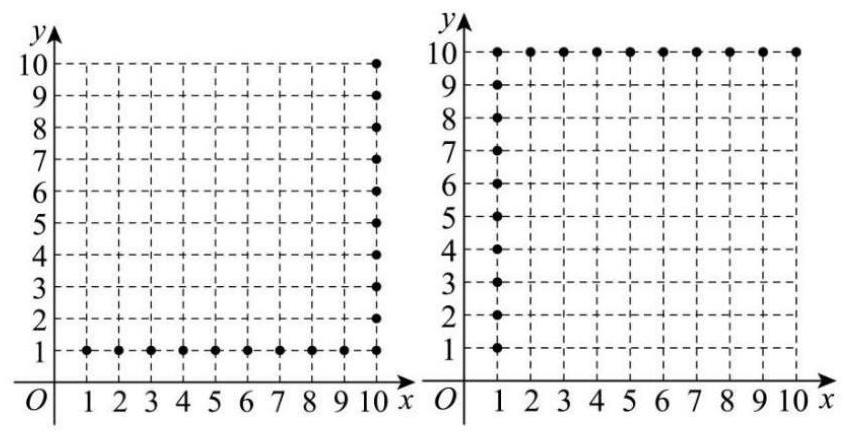
\includegraphics[max width=0.7\textwidth]{images/bo_d5jma53ef24c73bll4ig_6_295_792_845_433_0.jpg}
\end{center}
\hspace*{3em} 

【练习】2. 设集合 \(M = \{ 1,2,3,\cdots ,{2024},{2025}\} ,A\) 是 \(M\) 的子集且满足: 当 \(x \in  A\) 时, \({15x} \notin  A\) ,则 \(A\) 中元素最多有\_\_\_\_\_个。

【答案】 1899

【解析】2025 \(= {15} \times  {135}\) ,故取出所有不是 15 的倍数的数,共 1890 个,

这些数均符合要求,

因为 \({2025} \div  {15}^{2} = 9\) ,所以在所有 15 的倍数的数中, \({15}^{2}\) 的倍数有 9 个,

所以 1\textasciitilde 9 可以取出，这样共取出了 1899 个，故 \(A\) 中元素最多有 1899 个.

【练习】3. 设 \(a\text{ 、 }b\text{ 、 }c\text{ 、 }p\) 为实数，若同时满足不等式 \(a{x}^{2} + {bx} + c > 0\text{ 、 }b{x}^{2} + {cx} + a > 0\) 与 \(c{x}^{2} + {ax} + b >\) 0 的全体实数 \(x\) 所组成的集合等于 \(\left( {p, + \infty }\right)\) ,

则下列两个命题: \circled{1}  \(a\) 、 \(b\) 、 \(c\) 至少有一个为 0 ；  \circled{2}  \(p = 0\) .

下列判断正确的是 ( )

A.  \circled{1} 和 \circled{2} 都正确 B.  \circled{1} 和 \circled{2} 都错误 C.  \circled{1} 正确， \circled{2} 错误 D.  \circled{1} 错误， \circled{2} 正确

【答案】 \(A\)

【解析】若同时满足不等式 \(a{x}^{2} + {bx} + c > 0\text{ 、 }b{x}^{2} + {cx} + a > 0\) 与 \(c{x}^{2} + {ax} + b > 0\) 的

全体实数 \(x\) 所组成的集合等于 \(\left( {p, + \infty }\right)\) ,必有 \(a,b,c \geq  0\) ,

不妨假设 \(a\text{ 、 }b\text{ 、 }c\) 没有一个为 0,

则三个不等式均为开口向上的二次函数大于 0 的部分,

解集的交集应为 \(\left( {-\infty ,m}\right)  \cup  \left( {n, + \infty }\right)\) 的形式,矛盾,

所以 \(a\text{ 、 }b\text{ 、 }c\) 至少有一个为 0,故 \circled{1} 正确；

不妨设 \(a = 0\) ,则 \(b,c \geq  0\) ,则不等式组化为 \(\left\{  \begin{array}{l} {bx} + c > 0 \\  b{x}^{2} + {cx} > 0 \\  c{x}^{2} + b > 0 \end{array}\right.\) ,

所以 \(\left\{  \begin{array}{l} x >  - \frac{c}{b} \\  x <  - \frac{c}{b}\text{ 或 }x > 0 \\  x \in  R \end{array}\right.\) ,取交集得 \(\left( {0, + \infty }\right)\) ,故 \(p = 0\) ,故 \circled{2} 正确；

故选 \(A\) .

【练习】4. 已知等差数列 \(\left\{  {a}_{n}\right\}\) (公差不为零) 和等差数列 \(\left\{  {b}_{n}\right\}\) ,

如果关于 \(x\) 的方程 \({2025}{x}^{2} - \left( {{a}_{1} + {a}_{1} + \cdots  + {a}_{2025}}\right) x + {b}_{1} + {b}_{1} + \cdots  + {b}_{2025} = 0\) 有实数解,

那么以下 2025 个方程 \({x}^{2} - {a}_{1}x + {b}_{1} = 0,{x}^{2} - {a}_{2}x + {b}_{2} = 0,{x}^{2} - {a}_{3}x + {b}_{3} = 0,\cdots\) ,

\({x}^{2} - {a}_{2025}x + {b}_{2025} = 0\) 中,无实数解的方程最多有 ( )

A. 1011 个 B. 1012 个 C. 1013 个 D. 1014 个

【答案】 \(B\)

【解析】设等差数列 \(\left\{  {a}_{n}\right\}\) (公差 \({d}_{1}\) 不为零) 和等差数列 \(\left\{  {b}_{n}\right\}\) 的公差为 \({d}_{2}\) ,

则关于 \(x\) 的方程 \({2025}{x}^{2} - \left( {{a}_{1} + {a}_{1} + \cdots  + {a}_{2025}}\right) x + {b}_{1} + {b}_{1} + \cdots  + {b}_{2025} = 0\) 有实数解,

则 \({\left( {a}_{1} + {a}_{1} + \cdots  + {a}_{2025}\right) }^{2} - 4 \times  {2025}\left( {{b}_{1} + {b}_{1} + \cdots  + {b}_{2025}}\right)  \geq  0\) ,即 \({a}_{1013}^{2} \geq  4{b}_{1013}\) ,

则第 1013 个方程有解,记 2025 个方程的判别式为 \({\Delta }_{i} = {a}_{i}^{2} - 4{b}_{i}\left( {\mathrm{i} = 1,2,3,\cdots ,{2025}}\right)\)

则 \({\Delta }_{{1013} - i} + {\Delta }_{{1013} + i} = {\left( {a}_{1013} - i{d}_{1}\right) }^{2} + {\left( {a}_{1013} + i{d}_{1}\right) }^{2} - 8{b}_{1013} = 2\left( {{a}_{1013}^{2} - 4{b}_{1013}}\right)  + 2{\left( i{a}_{1}\right) }^{2} \geq\)

\(0\left( {\mathrm{i} = 1,2,3,\cdots ,{1012}}\right)\) ,所以每一对中至多一个负数,所以最多 1012 个方程无解,故选 \(C\) .

【练习】5. 若 \(a,b\) 是函数 \(f\left( x\right)  = {x}^{2} - {mx} + n\left( {m > 0,n > 0}\right)\) 的两个不同的零点,且 \(a,b, - 1\) 这三个数可适当排序后成等比数列,也可适当排序后成等差数列,则关于 \(x\) 的不等式 \(\frac{x - m}{x - n} \geq  0\) 的解集为 ( )

A. \(\{ x \mid  x \leq  2\) 或 \(x \geq  5\}\) B. \(\{ x \mid  x < 2\) 或 \(x \geq  5\}\)

C. \(\{ x \mid  x < 1\) 或 \(x \geq  \frac{5}{2}\}\) D. \(\left\{  {x\left| {\;x \leq  1}\right. }\right.\) 或 \(\left. {x > \frac{5}{2}}\right\}\)

【答案】 \(C\)

【解析】依题意,由 \(a,b\) 是函数 \(f\left( x\right)  = {x}^{2} - {mx} + n\left( {m > 0,n > 0}\right)\) 的两个不同的零点,

可知 \(a,b\) 是一元二次方程 \({x}^{2} - {mx} + n = 0\) 的两个不同的根,

由根据根与系数的关系,可得 \(a + b = m,{ab} = n\) ,

因为 \(m > 0,n > 0\) ,所以 \(a > 0,b > 0\) ,

又因为 \(a,b, - 1\) 这三个数可适当排序后成等比数列,

所以只有 -1 为该等比数列的等比中项才满足题意,

即 \({ab} = {\left( -1\right) }^{2} = 1 \Rightarrow  b = \frac{1}{a},n = 1\) ,

因为 \(a,b, - 1\) 这三个数可适当排序后成等差数列,

所以只有 -1 不能为该等差数列的中项,

 \circled{1} 当 \(a\) 为等差中项时，

根据等差中项的性质有 \({2a} = \frac{1}{a} - 1 \Rightarrow  a = \frac{1}{2},b = 2,m = \frac{5}{2}\) ,

 \circled{2}  当 \(\frac{1}{a}\) 为等差中项时，

根据等差中项的性质有 \(\frac{2}{a} = a - 1 \Rightarrow  a = 2,b = \frac{1}{2},m = \frac{5}{2}\) ,

综合 \circled{1}  \circled{2} ，可得 \(m = \frac{5}{2}\) ，

所以不等式 \(\frac{x - m}{x - n} \geq  0 \Leftrightarrow  \frac{x - \frac{5}{2}}{x - 1} \geq  0\) ,解得 \(x < 1\) 或 \(x \geq  \frac{5}{2}\) .

故选: \(C\)

\section*{板块三:压轴客观题}

\section*{1. 真题回顾}

【例题】1. (2024 上海秋考) 等比数列 \(\left\{  {a}_{n}\right\}\) 的首项 \({a}_{1} > 0\) ,公比 \(q > 1,{I}_{n} = \left\{  {x - y \mid  x,y \in  \left\lbrack  {{a}_{1},{a}_{2}}\right\rbrack   \cup  \left\lbrack  {{a}_{n},}\right. }\right. \; \left. \left. {a}_{n + 1}\right\rbrack  \right\}\) . 若对任意正整数 \(n\) ， \({I}_{n}\) 都是闭区间，则 \(q\) 的取值范围为\_\_\_\_\_.

【答案】 \(\lbrack 2, + \infty )\)

【解析】因为等比数列 \(\left\{  {a}_{n}\right\}\) 的首项 \({a}_{1} > 0\) ,公比 \(q > 1\) ,所以等比数列 \(\left\{  {a}_{n}\right\}\) 为严格增数列,

若 \(x,y \in  \left\lbrack  {{a}_{1},{a}_{2}}\right\rbrack\) ,则 \(x - y \in  \left\lbrack  {{a}_{1} - {a}_{2},{a}_{2} - {a}_{1}}\right\rbrack\)  \circled{1} ,

若 \(x,y \in  \left\lbrack  {{a}_{n},{a}_{n + 1}}\right\rbrack\) ,则 \(x - y \in  \left\lbrack  {{a}_{n} - {a}_{n + 1},{a}_{n + 1} - {a}_{n}}\right\rbrack\)  \circled{2} ,

若 \(x,y \in  \left\lbrack  {{a}_{1},{a}_{2}}\right\rbrack   \cup  \left\lbrack  {{a}_{n},{a}_{n + 1}}\right\rbrack\) ,则 \(- y \in  \left\lbrack  {-{a}_{n + 1}, - {a}_{n}}\right\rbrack   \cup  \left\lbrack  {-{a}_{2}, - {a}_{1}}\right\rbrack\) ,

所以 \(x - y \in  \left\lbrack  {{a}_{1} - {a}_{n + 1},{a}_{2} - {a}_{n}}\right\rbrack   \cup  \left\lbrack  {{a}_{n} - {a}_{2},{a}_{n + 1} - {a}_{1}}\right\rbrack\)  \circled{3} ,

由题意得 \circled{1}  \circled{2}  \circled{3} 组成的并集为闭区间，

注意到 \(\left( {{a}_{n + 1} - {a}_{n}}\right)  - \left( {{a}_{2} - {a}_{1}}\right)  = \left( {{a}_{n} - {a}_{1}}\right) \left( {q - 1}\right)  > 0\) ,所以 \circled{1} 和 \circled{2} 的并集就是 \circled{2} ，

只需要考虑 \circled{2}  \circled{3} 的并集，注意到 \circled{2} 和 \circled{3} 都是关于原点对称的区间，

且 \circled{3} 的右端点大于 \circled{2} 的右端点，那么只需要满足 \({a}_{n + 1} - {a}_{n} \geq  {a}_{n} - {a}_{2}\) ，

所以 \({q}^{n} - {q}^{n - 1} \geq  {q}^{n - 1} - q\) ,即 \({q}^{n} - 2{q}^{n - 1} \geq   - q\) 恒成立，所以 \(q - 2 \geq   - {q}^{2 - n}\) 恒成立，

所以 \(q - 2 \geq  0\) (对右边取极限),所以 \(q \geq  2\) ,所以 \(q\) 的取值范围为 \(\lbrack 2, + \infty )\) .

【例题】2. (2024 上海春考) 已知 \({a}_{1} = 2,{a}_{2} = 4,{a}_{3} = 8,{a}_{4} = {16}\) ,若存在实数 \({b}_{1},{b}_{2},{b}_{3},{b}_{4}\) ,满足 \(\left\{  {{a}_{i} + {a}_{j} \mid  1 \leq  \mathrm{i} < j \leq  4}\right\}   = \left\{  {{b}_{i} + {b}_{j} \mid  1 \leq  \mathrm{i} < j \leq  4}\right\}\) ,则有序实数组 \(\left\{  {{b}_{1},{b}_{2},{b}_{3},{b}_{4}}\right\}\) 的总个数为\_\_\_\_\_.

【答案】48

【解析】 \(\left\{  {{a}_{i} + {a}_{j} \mid  1 \leq  i < j \leq  4}\right\}   = \{ 6,{10},{12},{18},{20},{24}\}\) ,

不妨设 \({b}_{1} < {b}_{2} < {b}_{3} < {b}_{4}\) ,则 \({b}_{1} + {b}_{2} < {b}_{1} + {b}_{3} < \left\{  {\begin{array}{l} {b}_{1} + {b}_{4} \\  {b}_{2} + {b}_{3} \end{array} < {b}_{2} + {b}_{4} < {b}_{3} + {b}_{4}}\right.\) ,

按顺序对应, 分两种情况:

\({12} = {b}_{1} + {b}_{4} < {b}_{2} + {b}_{3} = {18}\) ,解得 \(\left\{  {{b}_{1},{b}_{2},{b}_{3},{b}_{4}}\right\}   = \{  - 1,7,{11},{13}\}\) ,

\({12} = {b}_{2} + {b}_{3} < {b}_{1} + {b}_{4} = {18}\) ,解得 \(\left\{  {{b}_{1},{b}_{2},{b}_{3},{b}_{4}}\right\}   = \{ 2,4,8,{16}\}\) ,

故有序实数组的总个数为 \(2{P}_{4}^{4} = {48}\) 组.

【例题】3. (2021 上海秋考) 已知两两不相等的 \({x}_{1}\text{ 、 }{y}_{1}\text{ 、 }{x}_{2}\text{ 、 }{y}_{2}\text{ 、 }{x}_{3}\text{ 、 }{y}_{3}\) ,同时满足 \(\text{  \circled{1}  }{x}_{1} < {y}_{1},{x}_{2} < {y}_{2},{x}_{3} < \; {y}_{3};\)  \circled{2}  \({x}_{1} + {y}_{1} = {x}_{2} + {y}_{2} = {x}_{3} + {y}_{3};\)  \circled{3}  \({x}_{1}{y}_{1} + {x}_{3}{y}_{3} = 2{x}_{2}{y}_{2}\) ，以下哪个选项恒成立 ( )

A. \(2{x}_{2} < {x}_{1} + {x}_{3}\) B. \(2{x}_{2} > {x}_{1} + {x}_{3}\) C. \({x}_{2}^{2} < {x}_{1}{x}_{3}\) D. \({x}_{2}^{2} > {x}_{1}{x}_{3}\)

【答案】 \(A\)

【解析】法一: 设 \({x}_{1} + {y}_{1} = {x}_{2} + {y}_{2} = {x}_{3} + {y}_{3} = {2m},\left\{  {\begin{array}{l} {x}_{1} = m - a \\  {y}_{1} = m + a \end{array},\left\{  {\begin{array}{l} {x}_{2} = m - b \\  {y}_{2} = m + b \end{array},\left\{  {\begin{array}{l} {x}_{3} = m - c \\  {y}_{3} = m + c \end{array},}\right. }\right. }\right.\)

由题意得 \(\left\{  \begin{array}{l} a \neq  b \neq  c \\  a,b,c > 0 \end{array}\right.\) ,且 \({m}^{2} - {a}^{2} + {m}^{2} - {c}^{2} = 2\left( {{m}^{2} - {b}^{2}}\right)  > 0\) ,则 \(\left\{  \begin{array}{l} {a}^{2} + {c}^{2} = 2{b}^{2} \\  {m}^{2} > {b}^{2} \end{array}\right.\) ,

则 \({x}_{1} + {x}_{3} - 2{x}_{2} = \left( {m - a}\right)  + \left( {m - c}\right)  - 2\left( {m - b}\right)  = {2b} - \left( {a + c}\right)\) ,

因为 \({\left( 2b\right) }^{2} - {\left( a + c\right) }^{2} = 2\left( {{a}^{2} + {c}^{2}}\right)  - {\left( a + c\right) }^{2} > 0\) ,

所以 \({x}_{1} + {x}_{3} - 2{x}_{2} = {2b} - \left( {a + c}\right)  > 0\) ,所以 \(A\) 项正确, \(B\) 错误.

\({x}_{1}{x}_{3} - {x}_{2}^{2} = \left( {m - a}\right) \left( {m - c}\right)  - {\left( m - b\right) }^{2} = \left( {{2b} - a - c}\right) m + {ac} - {b}^{2}\)

\begin{center}
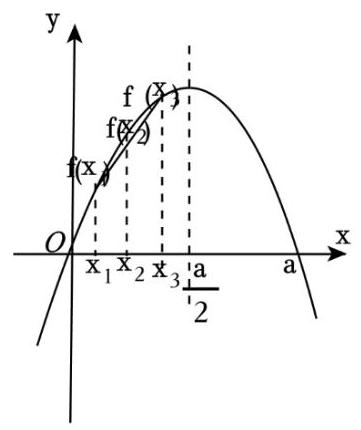
\includegraphics[max width=0.3\textwidth]{images/bo_d5jma53ef24c73bll4ig_10_1099_292_361_430_0.jpg}
\end{center}
\hspace*{3em} 

\(= \left( {{2b} - a - c}\right) m - \frac{{\left( a - c\right) }^{2}}{2}\) ,而上面已证 \(\left( {{2b} - a - c}\right)  > 0\) ,因为不知道 \(m\) 的正负,

所以该式子的正负无法恒定. 故选 \(A\) .

法二: 由于函数 \({x}_{1} + {y}_{1} = {x}_{2} + {y}_{2} = {x}_{3} + {y}_{3} = a\) ,则 \({x}_{1}{y}_{1} + {x}_{3}{y}_{3} = \; 2{x}_{2}{y}_{2}\) ,

即 \({x}_{1}\left( {a - {x}_{1}}\right)  + {x}_{3}\left( {a - {x}_{3}}\right)  = 2{x}_{2}\left( {a - {x}_{2}}\right)\) .

当 \(a > 0\) 时,由 \circled{1} 得 \({x}_{1} < \frac{a}{2},{x}_{2} < \frac{a}{2},{x}_{3} < \frac{a}{2}\) .

构造函数 \(f\left( x\right)  = x\left( {a - x}\right)\) ,则 \(f\left( {x}_{1}\right)  + f\left( {x}_{3}\right)  = {2f}\left( {x}_{2}\right)\) ,

设 \({x}_{1} < {x}_{2} < {x}_{3}\) ,作出 \(f\left( x\right)\) 的大致图象,

\(f\left( x\right)\) 为上凸函数,

有 \(f\left( \frac{{x}_{1} + {x}_{3}}{2}\right)  > \frac{f\left( {x}_{1}\right)  + f\left( {x}_{3}\right) }{2} = f\left( {x}_{2}\right)\) ,

函数 \(f\left( x\right)\) 在 \(\left( {-\infty ,\frac{a}{2}}\right)\) 上严格增,所以 \(\frac{{x}_{1} + {x}_{3}}{2} > {x}_{2}\) ,即 \(2{x}_{2} < {x}_{1} + {x}_{3}\) ,

当 \(a < 0\) 时,同理可得 \(2{x}_{2} < {x}_{1} + {x}_{3}\) . 故选 \(A\) . 2025 版上海高考真题及模拟训练合集

\section*{2. 模拟练习}

【练习】1. (2024 届华二) 已知两两不相等的正数 \({x}_{1}\text{ 、 }{y}_{1}\text{ 、 }{x}_{2}\text{ 、 }{y}_{2}\text{ 、 }{x}_{3}\text{ 、 }{y}_{3}\) ,同时满足 \circled{1}  \({x}_{1} < {y}_{1},{x}_{2} < {y}_{2},{x}_{3} \; < {y}_{3};\)  \circled{2}  \({x}_{1}{y}_{1} = {x}_{2}{y}_{2} = {x}_{3}{y}_{3};\)  \circled{3}  \(\left( {{x}_{1} + {y}_{1}}\right) \left( {{x}_{3} + {y}_{3}}\right)  = {\left( {x}_{2} + {y}_{2}\right) }^{2}\) ，则下列选项中恒成立的是( )

A. \(2{y}_{2} < {y}_{1} + {y}_{3}\) B. \(2{y}_{2} > {y}_{1} + {y}_{3}\) C. \({y}_{2}^{2} < {y}_{1}{y}_{3}\) D. \({y}_{2}^{2} > {y}_{1}{y}_{3}\)

【答案】 \(D\)

【解析】设 \({x}_{1}{y}_{1} = {x}_{2}{y}_{2} = {x}_{3}{y}_{3} = {a}^{2} > 0\) ,则 \({x}_{i} = \frac{a}{{q}_{i}},{y}_{i} = a{q}_{i}\) ,其中 \({q}_{i} > 1\left( {\mathrm{i} = 1,2,3}\right)\)

\(\left( {{x}_{1} + {y}_{1}}\right) \left( {{x}_{3} + {y}_{3}}\right)  = {\left( {x}_{2} + {y}_{2}\right) }^{2} \Rightarrow  \left( {\frac{1}{{q}_{1}} + 1}\right) \left( {\frac{1}{{q}_{3}} + 1}\right)  = {\left( \frac{1}{{q}_{2}} + 1\right) }^{2}\)

\(\Rightarrow  {q}_{1}{q}_{3} + \frac{1}{{q}_{1}{q}_{3}} + \left( {\frac{{q}_{3}}{{q}_{1}} + \frac{{q}_{1}}{{q}_{3}}}\right)  = {q}_{2}^{2} + \frac{1}{{q}_{2}^{2}} + 2\) ,因为 \(\frac{{q}_{3}}{{q}_{1}} + \frac{{q}_{1}}{{q}_{3}} > 2\) ,

所以 \({q}_{1}{q}_{3} + \frac{1}{{q}_{1}{q}_{3}} < {q}_{2}^{2} + \frac{1}{{q}_{2}^{2}}\) ,构造函数 \(f\left( x\right)  = x + \frac{1}{x},x \in  \left( {1, + \infty }\right)\) 严格增,

由 \(f\left( {q}_{2}^{2}\right)  > f\left( {{q}_{1}{q}_{3}}\right)\) ,所以 \({y}_{2}^{2} > {y}_{1}{y}_{3}\) ,故选 \(D\) .

【练习】2. (2025 届华二) 已知 \(q > 0\) ,对任意正整数 \(n\) ,令 \({J}_{n} = \left\{  {x + y \mid  x,y \in  \left\lbrack  {{q}^{n},{q}^{n + 1}}\right\rbrack   \cup  \left\lbrack  {{q}^{2n},{q}^{{2n} + 1}}\right\rbrack  }\right\}\) . 若存在 \(n\) ,使得 \({J}_{n} = \left\lbrack  {{a}_{n},{b}_{n}}\right\rbrack   \cup  \left\lbrack  {{c}_{n},{d}_{n}}\right\rbrack   \cup  \left\lbrack  {{x}_{n},{y}_{n}}\right\rbrack\) ,且 \({b}_{n} < {c}_{n},{d}_{n} < {x}_{n}\) ,则 \(q\) 的取值范围是\_\_\_\_\_.

【答案】 \(1 < q < 2\)

【解析】因为 \(n = 1\) 时, \(\left\lbrack  {q,{q}^{2}}\right\rbrack\) 是区间,所以 \(q > 1\) .

对 \(x\text{ 、 }y\) 的范围分类讨论,

得 \({J}_{n} = \left\lbrack  {2{q}^{n},2{q}^{n + 1}}\right\rbrack   \cup  \left\lbrack  {{q}^{n} + {q}^{2n},{q}^{n + 1} + {q}^{{2n} + 1}}\right\rbrack   \cup  \left\lbrack  {2{q}^{2n},2{q}^{{2n} + 1}}\right\rbrack\) ,

故存在 \(n\) 使得 \(2{q}^{n + 1} < {q}^{n} + {q}^{2n}\) 且 \({q}^{n + 1} + {q}^{{2n} + 1} < 2{q}^{2n}\) .

因为 \({q}^{n} + {q}^{2n} \geq  2{q}^{\frac{3n}{2}} > 2{q}^{n + 1}\left( {q > 1}\right)\) ,所以只需 \({q}^{n + 1} + {q}^{{2n} + 1} < 2{q}^{2n}\) .

这又等价于存在 \(n\) 使得 \(q < {q}^{n}\left( {2 - q}\right)\) ,于是 \(q < 2\) .

而当 \(1 < q < 2\) 时,故存在 \(n > {\log }_{q}\frac{q}{2 - q}\) ,使得要求被满足,故 \(1 < q < 2\) 所求.

【练习】3. 已知 \(a\text{ 、 }b\text{ 、 }c \in  R\) ,若关于 \(x\) 的不等式 \(0 \leq  x + \frac{a}{x} + b \leq  \frac{c}{x} - 1\) 的解集为 \(\left\lbrack  {{x}_{1},{x}_{2}}\right\rbrack   \cup  \left\{  {x}_{3}\right\} \; \left. {\left( {{x}_{3} > {x}_{2} > {x}_{1} > 0}\right) \text{ ,则 }}\right)\) ( )

A. 不存在有序数组 \(\left( {a,b,c}\right)\) ,使得 \({x}_{2} - {x}_{1} = 1\)

B. 存在唯一有序数组 \(\left( {a,b,c}\right)\) ,使得 \({x}_{2} - {x}_{1} = 1\)

C. 有且只有两组有序数组 \(\left( {a,b,c}\right)\) ,使得 \({x}_{2} - {x}_{1} = 1\)

D. 存在无穷多组有序数组 \(\left( {a,b,c}\right)\) ,使得 \({x}_{2} - {x}_{1} = 1\)

【答案】 \(D\)

【解析】因为不等式 \(0 \leq  x + \frac{a}{x} + b \leq  \frac{c}{x} - 1\) 的解集为 \(\left\lbrack  {{x}_{1},{x}_{2}}\right\rbrack   \cup  \left\{  {x}_{3}\right\}  \left( {{x}_{3} > {x}_{2} > {x}_{1} > 0}\right)\) ,

所以 \(0 \leq  {x}^{2} + {bx} + a \leq  c - x\) 在 \(\left\lbrack  {{x}_{1},{x}_{2}}\right\rbrack   \cup  \left\{  {x}_{3}\right\}\) 上成立,

假设 \({x}_{1} = m,{x}_{2} = m + 1,{x}_{3} = n\) ,

则 \(c - n = 0 = {n}^{2} + {bn} + a\) ,由 \({x}_{3}\) 为一个独立的数得出,

所以 \(n = c\) ,且 \(m + 1\) 与 \(n\) 为方程 \({x}^{2} + {bx} + a = 0\) 的两个根,

因为 \({x}_{3} > {x}_{2} > {x}_{1} > 0\) ,所以 \(- b = m + n + 1 = m + c + 1,a = {mn} + n = {mc} + c\) ,

所以 \(b =  - m - c - 1\) ,且点 \(\left( {{x}_{1},{x}_{1}{}^{2} + b{x}_{1} + a}\right)\) 为 \(y = {x}^{2} + {bx} + a\) 与 \(y = c - x\) 的左交点,

所以 \({m}^{2} + {bm} + a = c - m\) 且 \(b =  - m - c - 1,a = {mc} + c\) ,

故 \({m}^{2} + {bm} + a = {m}^{2} - {m}^{2} - {mc} - m + {mc} + c = c - m\) ,所以 \(c - m = c - m\) 恒成立,

所以不论 \(a\text{ 、 }b\text{ 、 }c\) 取何值, \({x}_{2} - {x}_{1} = 1\) 恒成立,

即存在无穷多组有序数组 \(\left( {a,b,c}\right)\) ,使得 \({x}_{2} - {x}_{1} = 1\) ,

故选项 \(A\text{ 、 }B\text{ 、 }C\) 错误,选项 \(D\) 正确. 故选 \(D\) .

【练习】4. (2024 届七宝) 对于一个有穷正整数数列 \(Q\) ,设其各项为 \({a}_{1},{a}_{2},\cdots ,{a}_{m}\) ,各项和为 \(S\left( Q\right)\) ,集合 \(\left\{  {\left( {\mathrm{i},j}\right)  \mid  {a}_{i} > {a}_{j},1 \leq  \mathrm{i} < j \leq  m}\right\}\) 中元素的个数为 \(T\left( Q\right)\) ,对所有满足 \(S\left( Q\right)  = {100}\) 的数列 \(Q\) ,则 \(T\left( Q\right)\) 的最大值为\_\_\_\_\_.

【答案】 1250

【解析】法一:先确定几个核心突破点:

 \circled{1} 在数列 \(Q\) 项数固定的情况下，若要 \(T\left( Q\right)\) 最大，则这个数列应当控制其为单调减；

 \circled{2}  考虑到数列的各项和为定值，为了让项数多一些，应当尽量让各项的数值小一些，因此必须让 \({a}_{m} = 1\) ;

 \circled{3} 对数列进行倒序分析，便呈现递增规律，为了让项数多一些，这些数列的项所取的数值应当逐渐 +1 (当然, 允许出现一些相同的项)

 \circled{4} 数值小的项，应当在数量上不小于数值大的项. 比如数列中有 4 项为 2、3 项为 1，或者有 4 项为1、3项为2，这样的情况下我们一定选择后者，因为各项和固定为100，而后者可以提高取值空间.

 \circled{5} 接下来做一个大胆的猜测，驱使所有项的取值只有 2 和 1 是最优解. 接下来进行验证，比如有 \(x\) 项 \(1,y\) 项 \(2,z\) 项 \(3\left( {x \geq  y \geq  z}\right)\) ,此时把某一项 3 化为一项 2 和一项 1,于是有 \(x + 1\) 项 \(1,y +\) 1 项 \(2,z - 1\) 项3,先不论大于等于 4 的这些项,单就取1,2,3的这些项,我们先做一个有序数组 \(\left( {\mathrm{i},j}\right)\) 的比较:

原: \({xy} + {xz} + {yz}\) ; 现: \(\left( {x + 1}\right) \left( {y + 1}\right)  + \left( {x + 1}\right) \left( {z - 1}\right)  + \left( {y + 1}\right) \left( {z - 1}\right)\) ;

现 - 原 \(= x + y + 1 - x + z - 1 + z - y - 1 = {2z} - 1 \geq  1\) .

除此以外,原来和现在数列中大于等于 4 的项未作任何变化,而取1,2,3的这些项的总项数增加了1 ，于是总的有序数组数量必定又会获得增加，因此猜测是合理且严谨的.

接下来进行最终计算:设设有穷数列 \(Q\) 由 \(x\) 个 2 和 \(y\) 个 1 组成，则有 \({2x} + y = {100}\) ，所以 \(T\left( Q\right) \; = {xy} = x\left( {{100} - {2x}}\right)  =  - 2{x}^{2} + {100x}\) ,当 \(x = {25}\) 时, \(T\left( Q\right)\) 取最大值 1250 .

法二:通过对条件分析可以确定下面几点:

 \circled{1}  有穷数列 \(Q\) 中存在大于 1 的项，否则此时 \(T\left( Q\right)  = 0\) ；

 \circled{2}  \({a}_{m} = 1\) ，否则 \({a}_{m}\) 将拆分成 \({a}_{m}\) 个 1 后 \(T\left( Q\right)\) 变大；

 \circled{3}  当 \(t = 1,2,\cdots m - 1\) 时，有 \({a}_{t} \geq  {a}_{t + 1}\) ，否则交换 \({a}_{t}\) ， \({a}_{t + 1}\) 顺序后 \(T\left( Q\right)\) 变为 \(T\left( Q\right)  + 1\) ，进一步有 \({a}_{t} - {a}_{t + 1} \in  \{ 0,1\}\) ,否则有 \({a}_{t} \geq  {a}_{t + 1} + 2\) ,此时将 \({a}_{t}\) 改为 \({a}_{t} - 1\) ,并在数列末尾添加一项 1,此时 \(T\left( Q\right)\) 变大;

 \circled{4}  各项只能为 2 和 1，否则通过拆分比 2 大的数调换位置后可使得 \(T\left( Q\right)\) 变大；

 \circled{5} 由上可得数列 \(Q\) 为 \(2,2,\cdots 2,1,1,\cdots 1\) 的形式，设有穷数列 \(Q\) 由 \(x\) 个 2 和 \(y\) 个 1 组成，则有 \({2x} + y = {100},\therefore T\left( Q\right)  = {xy} = x\left( {{100} - {2x}}\right)  =  - 2{x}^{2} + {100x}\) ,当 \(x = {25}\) 时, \(T\left( Q\right)\) 取最大值 1250 .

【练习】5. 已知函数 \(f\left( x\right)  = \cos x\) ,若对任意实数 \({x}_{1},{x}_{2}\) ,方程 \(\left| {f\left( x\right)  - f\left( {x}_{1}\right) }\right|  + \left| {f\left( x\right)  - f\left( {x}_{2}\right) }\right|  = m\left( {m \in  R}\right)\) 有解,方程 \(\left| {f\left( x\right)  - f\left( {x}_{1}\right) }\right|  - \left| {f\left( x\right)  - f\left( {x}_{2}\right) }\right|  = n\left( {n \in  R}\right)\) 也有解,则 \(m + n\) 的值的集合为\_\_\_\_\_.

【答案】 \{2\}

【解析】根据题意,不妨设 \(\cos {x}_{1} \leq  \cos {x}_{2}\) ,分类讨论当 \(\cos x \geq  \cos {x}_{2},\cos x \leq  \cos {x}_{1},\cos {x}_{1} < \cos x < \cos {x}_{2}\) 三种情况下,结合方程有解以及余弦函数的图象和性质,从而求出 \(m\) 和 \(n\) 的值,即可得出 \(m + \; n\) 的值的集合.

由题可知 \(f\left( x\right)  = \cos x\) ,不妨设 \(\cos {x}_{1} \leq  \cos {x}_{2}\) ,

对于 \(m\) ,对任意实数 \({x}_{1},{x}_{2}\) ,方程 \(\left| {f\left( x\right)  - f\left( {x}_{1}\right) }\right|  + \left| {f\left( x\right)  - f\left( {x}_{2}\right) }\right|  = m\left( {m \in  R}\right)\) 有解,

当 \(\cos x \geq  \cos {x}_{2}\) 时,方程可化为 \(m = 2\cos x - \left( {\cos {x}_{1} + \cos {x}_{2}}\right)\) 有解,

所以 \(m \geq  \cos {x}_{2} - \cos {x}_{1}\) 恒成立,所以 \(m \geq  2\) ;

当 \(\cos x \leq  \cos {x}_{1}\) 时，同上；

当 \(\cos {x}_{1} < \cos x < \cos {x}_{2}\) 时，方程可化为 \(m = \cos {x}_{2} - \cos {x}_{1}\) 有解，所以 \(m \in  \left\lbrack  {0,2}\right\rbrack\) ，

综上得: \(m = 2\) ;

对于 \(n\) ,对任意实数 \({x}_{1},{x}_{2}\) ,方程 \(\left| {f\left( x\right)  - f\left( {x}_{1}\right) }\right|  - \left| {f\left( x\right)  - f\left( {x}_{2}\right) }\right|  = n\left( {n \in  R}\right)\) 也有解,

当 \(\cos x \geq  \cos {x}_{2}\) 时,方程可化为 \(n = \cos {x}_{2} - \cos {x}_{1}\) 有解,所以 \(n \in  \left\lbrack  {0,2}\right\rbrack\) ;

当 \(\cos x \leq  \cos {x}_{1}\) 时，同上；

当 \(\cos {x}_{1} < \cos x < \cos {x}_{2}\) 时,方程可化为 \(n = 2\cos x - \left( {\cos {x}_{2} + \cos {x}_{1}}\right)\) 有解,

所以 \(\cos {x}_{1} - \cos {x}_{2} < n < \cos {x}_{2} - \cos {x}_{1}\) 恒成立,所以 \(n = 0\) ,

所以 \(m + n\) 的值的集合为 \(\{ 2\}\) .

故答案为: \(\{ 2\}\) .

【练习】6. 设 \({x}_{1},{x}_{2},{x}_{3},{x}_{4} \in  \left( {0,\frac{\pi }{2}}\right)\) ,则 ( )

A. 在这四个数中至少存在两个数 \(x,y\) ,满足 \(\sin \left( {x - y}\right)  > \frac{1}{2}\)

B. 在这四个数中至少存在两个数 \(x,y\) ,满足 \(\cos \left( {x - y}\right)  \geq  \frac{\sqrt{3}}{2}\)

C. 在这四个数中至多存在两个数 \(x,y\) ,满足 \(\tan \left( {x - y}\right)  < \frac{\sqrt{3}}{3}\)

D. 在这四个数中至多存在两个数 \(x,y\) ,满足 \(\sin \left( {x - y}\right)  \geq  \frac{1}{2}\)

【答案】 \(B\)

【解析】将区间 \(\left( {0,\frac{\pi }{2}}\right)\) 平均分为三个区间,则每个区间的长度为 \(\frac{\pi }{6}\) . 因为 \({x}_{1},{x}_{2},{x}_{3},{x}_{4} \in  \left( {0,\frac{\pi }{2}}\right)\) ,所以在 \({x}_{1},{x}_{2},{x}_{3},{x}_{4}\) 中至少有两个数在同一区间内,设这两个数为 \(x,y\) ,则 \(\left| {x - y}\right|  \leq  \frac{\pi }{6}\) ,又因为 \(y \; = \sin x\) 在 \(\left( {0,\frac{\pi }{2}}\right)\) 上单调递增, \(y = \cos x\) 在 \(\left( {0,\frac{\pi }{2}}\right)\) 上单调递减,所以 \(\sin \left( {x - y}\right)  \leq  \frac{1}{2},\cos (x - \; y) \geq  \frac{\sqrt{3}}{2}\) ,故 \(A\) 错误, \(B\) 正确;

对于 \(C\) : 取 \({x}_{1} = {x}_{2} = {x}_{3} = {x}_{4} = \frac{\pi }{6},\tan \left( {{x}_{2} - {x}_{1}}\right)  = \tan \left( {{x}_{4} - {x}_{3}}\right)  = 0\) ,故 \(C\) 错误;

对于 \(D\) : 取 \({x}_{1} = \frac{\pi }{12},{x}_{2} = \frac{\pi }{6},{x}_{3} = \frac{\pi }{4},{x}_{4} = \frac{\pi }{3},\sin \left( {{x}_{4} - {x}_{2}}\right)  = \sin \left( {{x}_{3} - {x}_{1}}\right)  = \frac{1}{2}\) ,故 \(D\) 错误;

故选: \(B\) .

【练习】7. 已知 \({x}_{1}\text{ 、 }{x}_{2}\text{ 、 }\cdots \text{ 、 }{x}_{2023}\) 均为正数,并且 \(\frac{1}{1 + {x}_{1}} + \frac{1}{1 + {x}_{2}} + \cdots  + \frac{1}{1 + {x}_{2023}} = 1\) ,给出下列四个结论:

 \circled{1}  \({x}_{1}\) 、 \({x}_{2}\) 、 \(\cdots\) 、 \({x}_{2023}\) 中小于 1 的数最多只有一个;

 \circled{2}  \({x}_{1}\) 、 \({x}_{2}\) 、 \(\cdots\) 、 \({x}_{2023}\) 中小于 2 的数最多只有两个;

 \circled{3}  \({x}_{1}\text{ 、 }{x}_{2}\text{ 、 }\cdots \text{ 、 }{x}_{2023}\) 中最大的数不小于 2022;

 \circled{4}  \({x}_{1}\text{ 、 }{x}_{2}\text{ 、 }\cdots \text{ 、 }{x}_{2023}\) 中最小的数不小于 \(\frac{1}{2023}\) .

其中所有正确结论的序号为\_\_\_\_\_.

【答案】 \circled{1}  \circled{2}  \circled{3} 

【解析】对于 \circled{1} ,假设在 \({x}_{1}\text{ 、 }{x}_{2}\text{ 、 }\cdots \text{ 、 }{x}_{2023}\) 中有 2 个或更多的数小于 1,

不妨设 \(0 < {x}_{1} < 1,0 < {x}_{2} < 1,\frac{1}{1 + {x}_{1}} > \frac{1}{2},\frac{1}{1 + {x}_{2}} > \frac{1}{2}\) ,

则有 \(\frac{1}{1 + {x}_{1}} + \frac{1}{1 + {x}_{2}} + \cdots  + \frac{1}{1 + {x}_{2023}} > \frac{1}{2} + \frac{1}{2} = 1\) ,

故假设不成立,则 \({x}_{1}\text{ 、 }{x}_{2}\text{ 、 }\cdots \text{ 、 }{x}_{2023}\) 中小于 1 的数最多只有一个, \circled{1} 正确；

对于 \circled{2} ，假设在 \({x}_{1}\) 、 \({x}_{2}\) 、 \(\cdots\) 、 \({x}_{2023}\) 中有 3 个或更多的数小于 2，

不妨设 \(0 < {x}_{1} < 2,0 < {x}_{2} < 2,0 < {x}_{3} < 2\) ,

则 \(\frac{1}{1 + {x}_{1}} > \frac{1}{3},\frac{1}{1 + {x}_{2}} > \frac{1}{3},\frac{1}{1 + {x}_{3}} > \frac{1}{3}\) ,

则有 \(\frac{1}{1 + {x}_{1}} + \frac{1}{1 + {x}_{2}} + \cdots  + \frac{1}{1 + {x}_{2023}} > \frac{1}{3} + \frac{1}{3} + \frac{1}{3} = 1\) ,

故假设不成立，则 \({x}_{1}\) 、 \({x}_{2}\) 、、、 \({x}_{2023}\) 中小于 2 的数最多只有两个， \circled{2} 正确；

对于 \circled{3} ，假设 \({x}_{1}\) 、 \({x}_{2}\) 、 \(\cdots\) 、 \({x}_{2023}\) 中最大的数小于 2022，

即 \(0 < {x}_{1} < {2022}\text{ 、 }0 < {x}_{2} < {2022}\text{ 、 }\cdots \text{ 、 }0 < {x}_{2013} < {2022}\) ,

则 \(\frac{1}{1 + {x}_{1}} > \frac{1}{2023}\text{ 、 }\frac{1}{1 + {x}_{2}} > \frac{1}{2023}\text{ 、 }\cdots \text{ 、 }\frac{1}{1 + {x}_{2023}} > \frac{1}{2023}\) ,

显然 \(\frac{1}{1 + {x}_{1}} + \frac{1}{1 + {x}_{2}} + \cdots  + \frac{1}{1 + {x}_{2023}} > {2023} \times  \frac{1}{2023} = 1\) ,

故假设不成立，则 \({x}_{1}\) 、 \({x}_{2}\) 、 \(\cdots\) 、 \({x}_{2023}\) 中最大的数不小于 2022, \circled{3}  正确；

对于 \circled{4} ，假设 \({x}_{1}\) 是 \({x}_{1}\) 、 \({x}_{2}\) 、 \(\cdots\) 、 \({x}_{2023}\) 中最小的数，

当 \({x}_{1} = \frac{1}{2024}\) ,其余 \({x}_{2} = \cdots  = {x}_{2023} = {2025} \times  {2022} - 1\) 时,满足 \({x}_{1} < \frac{1}{2023}\) ,

此时 \(\frac{1}{1 + {x}_{1}} + \frac{1}{1 + {x}_{2}} + \cdots  + \frac{1}{1 + {x}_{2023}}\)

\(= \frac{1}{1 + \frac{1}{2024}} + {2022} \times  \frac{1}{{2025} \times  {2022}} = \frac{2024}{2025} + \frac{1}{2025} = 1\) ,故 \circled{4} 错误.

故正确结论的序号为 \circled{1}  \circled{2}  \circled{3} .

【练习】8. (2024 届格致) 已知非空集合 \(A \subseteq  R\) ,设集合 \(S = \{ x + y \mid  x \in  A,y \in  A\) 且 \(x \neq  y\}\) , \(T = \{ x - y \mid  x \in  A,y \in  A\) 且 \(x > y\}\) . 分别用 \(\left| A\right| \text{ 、 }\left| S\right| \text{ 、 }\left| T\right|\) 表示集合 \(A\text{ 、 }S\text{ 、 }T\) 中元素的个数,则下列说法不正确的是 ( )

A. 若 \(\left| A\right|  = 4\) ,则 \(\left| S\right|  + \left| T\right|  \geq  8\) B. 若 \(\left| A\right|  = 4\) ,则 \(\left| S\right|  + \left| T\right|  \leq  {12}\)

C. 若 \(\left| A\right|  = 5\) ,则 \(\left| S\right|  + \left| T\right|\) 可能为 18 D. 若 \(\left| A\right|  = 5\) ,则 \(\left| S\right|  + \left| T\right|\) 不可能为 19

【答案】 \(D\)

【解析】当 \(\left| A\right|  = 4\) 时,分两种情况如下,

不考虑重复情况时: \(\left| S\right|  \leq  {C}_{4}^{2} = 6,\left| T\right|  \leq  {C}_{4}^{2} = 6\) ,所以 \(\left| S\right|  + \left| T\right|  \leq  {12}\) ,

考虑重复情况时: 例如 \(A = \{ 1,2,3,4\}\) ,

\(S = \{ 3,4,5,6,7\} ,T = \{ 1,2,3\}\) ,所以 \(\left| S\right|  + \left| T\right|  \geq  8\) ,所以 \(A\text{ 、 }B\) 正确.

当 \(\left| A\right|  = 5\) 时,分两种情况如下,

不考虑重复情况时, \(\left| S\right|  \leq  {C}_{5}^{2} = {10},\left| T\right|  \leq  {C}_{5}^{2} = {10}\) ,所以 \(\left| S\right|  + \left| T\right|  \leq  {20}\) ,

考虑重复情况时,例如 \(A = \{ 1,2,3,5,{10}\}\) ,

\(S = \{ 3,4,5,6,7,8,{11},{12},{13},{15}\} ,T = \{ 1,2,3,4,5,7,8,9\}\) ,所以 \(\left| S\right|  + \left| T\right|  = {18},C\) 正确, 例如 \(A = \{ 1,2,4,6,{16}\}\) ,

\(S = \{ 3,5,6,7,8,{10},{17},{18},{20},{22}\} ,T = \{ 1,2,3,4,5,{10},{12},{14},{15}\}\) ,所以 \(\left| S\right|  + \left| T\right|  = {19}\) , \(D\) 不正确. 故选 \(D\) .

\section*{口二、函数与导数}

\section*{板块一:基础客观题}

1. 真题回顾

【例题】1. (2024 上海春考)已知 \(f\left( x\right)  = {x}^{2},g\left( x\right)  = \left\{  \begin{array}{ll} f\left( x\right) , & x \geq  0 \\   - f\left( {-x}\right) , & x < 0 \end{array}\right.\) ，则 \(g\left( x\right)  \leq  2 - x\) 的解集为\_\_\_\_\_.

【答案】 \(( - \infty ,1\rbrack\)

【解析】 \(g\left( x\right)  = \left\{  {\begin{array}{ll} {x}^{2}, & x \geq  0 \\   - {x}^{2}, & x < 0 \end{array},g\left( x\right)  \leq  2 - x}\right.\) ,

当 \(x \geq  0\) 时, \({x}^{2} + x - 2 \leq  0\) ,解得 \(x \in  \left\lbrack  {0,1}\right\rbrack\) ;,

当 \(x < 0\) 时, \(- {x}^{2} + x - 2 \leq  0\) ,解得 \(x \in  \left( {-\infty ,0}\right)\) ;,

综上,解集为 \(( - \infty ,1\rbrack\) .

【例题】2. (2022 上海秋考) 若函数 \(f\left( x\right)  = \left\{  \begin{array}{ll} {a}^{2}x - 1, & x < 0 \\  x + a, & x > 0 \\  0, & x = 0 \end{array}\right.\) 为奇函数,则实数 \(a =\) \_\_\_\_\_.

【答案】1

【解析】法一: 由 \(f\left( 1\right)  + f\left( {-1}\right)  = 0\) 得 \(1 + a - {a}^{2} - 1 = 0\) ,所以 \(a = 0\) 或1,经检验 \(a = 1\) .

法二: 当 \(x < 0\) 时, \(- x > 0\) ,由 \(f\left( x\right)  + f\left( {-x}\right)  = 0\) 得 \({a}^{2}x - 1 - x + a = 0\) ,

即 \(\left( {{a}^{2} - a}\right) x + \left( {a - 1}\right)  = 0\) ,即 \(\left( {a - 1}\right) \left( {{ax} + 1}\right)  = 0\) ,所以 \(a = 1\) .

【例题】3. (2014 上海秋考) 设 \(f\left( x\right)  = \left\{  \begin{array}{ll} {\left( x - a\right) }^{2}, & x \leq  0 \\  x + \frac{1}{x} + a, & x > 0 \end{array}\right.\) ,若 \(f\left( 0\right)\) 是 \(f\left( x\right)\) 的最小值,则 \(a\) 的取值范围为 ( )

A. \(\left\lbrack  {-1,2}\right\rbrack\) B. \(\left\lbrack  {-1,0}\right\rbrack\) C. \(\left\lbrack  {1,2}\right\rbrack\) D. \(\left\lbrack  {0,2}\right\rbrack\)

【答案】 \(D\)

【解析】当 \(a < 0\) 时,显然 \(f\left( 0\right)\) 不是 \(f\left( x\right)\) 的最小值,

当 \(a \geq  0\) 时, \(f\left( 0\right)  = {a}^{2}\) ,由题意得 \({a}^{2} \leq  x + \frac{1}{x} + a\) ,

解不等式 \({a}^{2} - a - 2 \leq  0\) ,得 \(- 1 \leq  a \leq  2\) ,所以 \(0 \leq  a \leq  2\) ,故选 \(D\) .

【例题】4. (2013 上海秋考) 设 \(a\) 为实常数, \(y = f\left( x\right)\) 是定义在 \(R\) 上的奇函数,当 \(x < 0\) 时, \(f\left( x\right)  = {9x} + \; \frac{{a}^{2}}{x} + 7\) . 若 \(f\left( x\right)  \geq  a + 1\) 对一切 \(x \geq  0\) 成立，则 \(a\) 的取值范围为\_\_\_\_\_.

【答案】 \(\left( {-\infty , - \frac{8}{7}}\right\rbrack\)

【解析】因为 \(y = f\left( x\right)\) 是定义在 \(R\) 上的奇函数,所以当 \(x = 0\) 时, \(f\left( x\right)  = 0\) ;

当 \(x > 0\) 时,则 \(- x < 0\) ,所以 \(f\left( {-x}\right)  =  - {9x} - \frac{{a}^{2}}{x} + 7\) ,

因为 \(y = f\left( x\right)\) 是定义在 \(R\) 上的奇函数,所以 \(f\left( x\right)  = {9x} + \frac{{a}^{2}}{x} - 7\) ,

因为 \(f\left( x\right)  \geq  a + 1\) 对一切 \(x \geq  0\) 成立，所以当 \(x = 0\) 时， \(0 \geq  a + 1\) 成立，所以 \(a \leq   - 1\) ；

当 \(x > 0\) 时， \({9x} + \frac{{a}^{2}}{x} - 7 \geq  a + 1\) 成立，只需要 \({9x} + \frac{{a}^{2}}{x} - 7\) 的最小值 \(\geq  a + 1\) ，

因为 \({9x} + \frac{{a}^{2}}{x} - 7 \geq  2\sqrt{{9x} \cdot  \frac{{a}^{2}}{x}} - 7 = 6\left| a\right|  - 7\) ,所以 \(6\left| a\right|  - 7 \geq  a + 1\) ,

解得 \(a \geq  \frac{8}{5}\) 或 \(a \leq   - \frac{8}{7}\) ，所以 \(a \leq   - \frac{8}{7}\) ，所以 \(a\) 的取值范围为 \(\left( {-\infty , - \frac{8}{7}}\right\rbrack\) .

【例题】5. (2011 上海秋考) 设 \(g\left( x\right)\) 是定义在 \(R\) 上,以 1 为周期的函数,若函数 \(f\left( x\right)  = x + g\left( x\right)\) 在区间 \(\left\lbrack  {3,4}\right\rbrack\) 上的值域为 \(\left\lbrack  {-2,5}\right\rbrack\) ，则 \(f\left( x\right)\) 在区间 \(\left\lbrack  {-{10},{10}}\right\rbrack\) 上的值域为\_\_\_\_\_.

【答案】 \(\left\lbrack  {-{15},{11}}\right\rbrack\)

【解析】法一:因为 \(g\left( x\right)\) 为 \(R\) 上周期为 1 的函数,则 \(g\left( x\right)  = g\left( {x + 1}\right)\) ,

又因为函数 \(f\left( x\right)  = x + g\left( x\right)\) 在 \(\left\lbrack  {3,4}\right\rbrack\) 的值域是 \(\left\lbrack  {-2,5}\right\rbrack\) ,

令 \(x + 6 = t\) ,当 \(x \in  \left\lbrack  {3,4}\right\rbrack\) 时, \(t = x + 6 \in  \left\lbrack  {9,{10}}\right\rbrack\) ,

此时 \(f\left( t\right)  = t + g\left( t\right)  = \left( {x + 6}\right)  + g\left( {x + 6}\right)  = \left( {x + 6}\right)  + g\left( x\right)  = \left\lbrack  {x + g\left( x\right) }\right\rbrack   + 6\) ,

所以在 \(t \in  \left\lbrack  {9,{10}}\right\rbrack\) 时, \(f\left( t\right)  \in  \left\lbrack  {4,{11}}\right\rbrack\)  \circled{1} ,

同理令 \(x - {13} = t\) ,在当 \(x \in  \left\lbrack  {3,4}\right\rbrack\) 时, \(t = x - {13} \in  \left\lbrack  {-{10}, - 9}\right\rbrack\) ,

此时, \(f\left( t\right)  = t + g\left( t\right)  = \left( {x - {13}}\right)  + g\left( {x - {13}}\right)  = \left( {x - {13}}\right)  + g\left( x\right)  = \left\lbrack  {x + g\left( x\right) }\right\rbrack   - {13}\) ,

所以,当 \(t \in  \left\lbrack  {-{10}, - 9}\right\rbrack\) 时, \(f\left( t\right)  \in  \left\lbrack  {-{15}, - 8}\right\rbrack\)  \circled{2} ,

...

由 \circled{1}  \circled{2} ...得到， \(f\left( x\right)\) 在 \(\left\lbrack  {-{10},{10}}\right\rbrack\) 上的值域为 \(\left\lbrack  {-{15},{11}}\right\rbrack\) .

法二: 由题意 \(f\left( x\right)  - x = g\left( x\right)\) 在 \(R\) 上成立,

故 \(f\left( {x + 1}\right)  - \left( {x + 1}\right)  = g\left( {x + 1}\right)\) ,所以 \(f\left( {x + 1}\right)  - f\left( x\right)  = 1\) ,

由此得自变量增大 1 , 函数值也增大 1 ,

故 \(f\left( x\right)\) 在 \(\left\lbrack  {-{10},{10}}\right\rbrack\) 上的值域为 \(\left\lbrack  {-{15},{11}}\right\rbrack\) .

【例题】6. (2010 上海春考)已知函数 \(f\left( x\right)  = \frac{1}{4 - {2}^{x}}\) 的图象关于点 \(P\) 对称，则点 \(P\) 的坐标是\_\_\_\_\_ ( )

A. \(\left( {2,\frac{1}{2}}\right)\) B. \(\left( {2,\frac{1}{4}}\right)\) C. \(\left( {2,\frac{1}{8}}\right)\) D. \(\left( {0,0}\right)\)

【答案】 \(C\)

【解析】设 \(P\left( {m,n}\right)\) ,任意给点 \(M\left( {x,y}\right)\) 关于 \(P\left( {m,n}\right)\) 的对称点为 \(N\left( {{2m} - x,{2n} - y}\right)\) ,

由 \(y = f\left( x\right)  = \frac{1}{4 - {2}^{x}},{2n} - y = f\left( {{2m} - x}\right)  = \frac{1}{4 - {2}^{{2m} - x}}\) ,

得 \(\left\{  \begin{array}{l} y = \frac{1}{4 - {2}^{x}} \\  {2n} - y = \frac{1}{4 - {2}^{{2m} - x}} \end{array}\right.\) ,解得 \(m = 2,n = \frac{1}{8}\) ,故选 \(C\) . 2025 版上海高考真题及模拟训练合集

\section*{2. 模拟练习}

【练习】1. (2025 届交附) 设 \(y = f\left( x\right)\) 与 \(y = g\left( x\right)\) 是两个不同的幂函数,记 \(M = \{ x \mid  f\left( x\right)  = g\left( x\right) \}\) ,则 \(M\) 中的元素个数的可能是 ( )

A. \(0\text{ 、 }1\text{ 、 }2\) B. \(1\text{ 、 }2\text{ 、 }3\) C. \(1\text{ 、 }2\text{ 、 }3\text{ 、 }4\) D. \(0\text{ 、 }1\text{ 、 }2\text{ 、 }3\)

【答案】 \(B\)

【解析】设 \(f\left( x\right)  = {x}^{a},g\left( x\right)  = {x}^{b}\) ,

 \circled{1}  由幂函数图像得 \(f\left( 1\right)  = g\left( 1\right)  = 1\) ，故 \(f\left( x\right)  = g\left( x\right)\) 至少存在一个解 \(x = 1\) ；

 \circled{2} 若 \(f\left( x\right) ,g\left( x\right)\) 在 0 处都有定义，则 \(f\left( 0\right)  = g\left( 0\right)  = 0\) ，

故 \(f\left( x\right)  = g\left( x\right)\) 可能存在解 \(x = 0\) ；

 \circled{3} 若 \(f\left( x\right) ,g\left( x\right)\) 同为奇函数或者偶函数，

由对称性得 \(f\left( {-1}\right)  = g\left( {-1}\right)  = 1\) 或 \(f\left( {-1}\right)  = g\left( {-1}\right)  =  - 1\) ,

故 \(f\left( x\right)  = g\left( x\right)\) 可能存在解 \(x =  - 1\) ,

综上所述， \(M\) 中的元素个数的可能是1,2,3. 故选 \(B\)

【练习】2. 关于 \(x\) 的不等式 \(\frac{1}{x} - {\log }_{2}x < 1\) 的解集为\_\_\_\_\_.

【答案】 \(\left( {1, + \infty }\right)\)

【解析】设 \(f\left( x\right)  = \frac{1}{x} - {\log }_{2}x\) ,且 \(f\left( x\right)\) 单调递减, \(f\left( 1\right)  = 1\) ,则 \(f\left( x\right)  < f\left( 1\right)  \Rightarrow  x > 1\) , 故解集为 \(\left( {1, + \infty }\right)\) .

【练习】3. (2025 届交附) 满足定义域为 \(\{ 1,2,3,4\}\) 且值域为 \(\{ 1,2,3\}\) 的函数共有\_\_\_\_\_个

【答案】36

【解析】 \({C}_{4}^{2}{P}_{3}^{3} = {36}\) 个

【练习】4. (2025 届交附) 已知 \(f\left( x\right)  = \left( {x + 1}\right) \left( {x + a}\right) \left( {x + b}\right)\) . 若 \(y = f\left( x\right)\) 为奇函数，则 \({f}^{\prime }\left( 0\right)  =\) \_\_\_\_\_

【答案】-1

【解析】 \(f\left( x\right)  = \left( {x + 1}\right) \left( {x + a}\right) \left( {x + b}\right)  = {x}^{3} + \left( {a + b + 1}\right) {x}^{2} + \left( {a + b + {ab}}\right) x + {ab}\) 为奇函数,

所以 \(\left\{  \begin{array}{l} a + b + 1 = 0 \\  {ab} = 0 \end{array}\right.\) ,解得 \(\left\{  \begin{array}{l} a = 0 \\  b =  - 1 \end{array}\right.\) 或 \(\left\{  \begin{array}{l} a =  - 1 \\  b = 0 \end{array}\right.\) ,所以 \(f\left( x\right)  = {x}^{3} - x\) ,

则 \({f}^{\prime }\left( x\right)  = 3{x}^{2} - 1\) ,则 \({f}^{\prime }\left( 0\right)  =  - 1\)

【练习】5. (2025 届交附) 设 \(f\left( x\right)  = \sqrt{a{x}^{2} + {bx} + c}\left( {a,b,c\text{ 为常数且 }a < 0}\right)\) . 集合 \(D\) 为使得 \(f\left( x\right)\) 有意义的实数集合,若集合 \(\{ \left( {s,f\left( t\right) }\right)  \mid  s,t \in  D\}\) 在平面直角坐标系内的图形是一个正方形区域,则实数 \(a\) 的值为\_\_\_\_\_

【答案】-4

【解析】由题意得定义域和值域长度相等,所以 \(\left| {{x}_{1} - {x}_{2}}\right|  = f{\left( x\right) }_{\max }\) ,

所以 \(\frac{\sqrt{{b}^{2} - {4ac}}}{-a} = \sqrt{\frac{{4ac} - {b}^{2}}{4a}}\) ,所以 \(a =  - 4\)

【练习】6. 已知函数 \(f\left( x\right)  = \left\{  \begin{array}{l} x - 1,x > a \\  a{x}^{2} + {2x} - 3,x \leq  a \end{array}\right.\) ,若 \(f\left( x\right)\) 有且只有 1 个极值点,则 \(a\) 的取值范围是\_\_\_\_\_.

【答案】 \(\left( {0, + \infty }\right)\)

【解析】当 \(a = 0\) 时,没有极值点;

当 \(a \neq  0\) 时, \({f}^{\prime }\left( x\right)  = \left\{  \begin{array}{l} 1,x > a \\  {2ax} + 2,x \leq  a \end{array}\right.\) ,取 \({2ax} + 2 = 0\) ,得到 \(x =  - \frac{1}{a}\) ,

当 \(x \leq  a\) 时，函数为二次函数，则 \(- \frac{1}{a} \leq  a\) ，故 \(a > 0\) ，

综上所述， \(a \in  \left( {0, + \infty }\right)\) .

\begin{center}
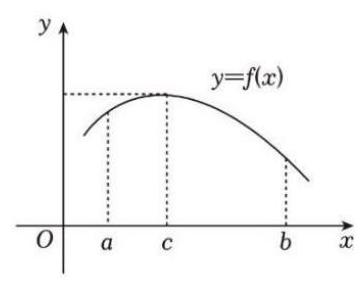
\includegraphics[max width=0.3\textwidth]{images/bo_d5jma53ef24c73bll4ig_19_1086_506_363_282_0.jpg}
\end{center}
\hspace*{3em} 

【练习】7. 已知 \(f\left( x\right)\) 的导数存在， \(y = f\left( x\right)\) 的图象如图所示，设 \(S\left( t\right) \left( {a \leq  t \leq  b}\right)\) 是由曲线 \(y = f\left( x\right)\) 与直线 \(x = a,x = t\) 及 \(x\) 轴围成的平面图形的面积,则在区间 \(\left\lbrack  {a,b}\right\rbrack\) 上( )

A. \({f}^{\prime }\left( x\right)\) 的最大值是 \({f}^{\prime }\left( a\right)\) ,最小值是 \({f}^{\prime }\left( c\right)\)

B. \({f}^{\prime }\left( x\right)\) 的最大值是 \({f}^{\prime }\left( c\right)\) ,最小值是 \({f}^{\prime }\left( b\right)\)

C. \({S}^{\prime }\left( t\right)\) 的最大值是 \({S}^{\prime }\left( a\right)\) ,最小值是 \({S}^{\prime }\left( c\right)\)

D. \({S}^{\prime }\left( t\right)\) 的最大值是 \({S}^{\prime }\left( c\right)\) ,最小值是 \({S}^{\prime }\left( b\right)\)

【答案】 \(D\)

【解析】如图所示, \({f}^{\prime }\left( x\right)\) 的最大值为 \({f}^{\prime }\left( a\right)\) ,最小值为 \({f}^{\prime }\left( b\right)\) .

由导数的定义得 \({S}^{\prime }\left( t\right)  = \mathop{\lim }\limits_{{{\Delta t} \rightarrow  0}}\frac{S\left( {t + {\Delta t}}\right)  - S\left( t\right) }{\Delta t} = \mathop{\lim }\limits_{{{\Delta t} \rightarrow  0}}\frac{{\Delta t} \cdot  f\left( t\right) }{\Delta t} = \mathop{\lim }\limits_{{{\Delta t} \rightarrow  0}}f\left( t\right)  = f\left( t\right)\) .

则 \({S}^{\prime }\left( t\right)\) 的最大值是 \({S}^{\prime }\left( c\right)\) ,最小值是 \({S}^{\prime }\left( b\right)\) ,故选 \(D\) .

【练习】8. 已知函数 \(f\left( x\right)  = \left( {x - 1}\right) {\mathrm{e}}^{x} - {mx}\) 在区间 \(x \in  \left\lbrack  {1,2}\right\rbrack\) 上存在严格增区间,则 \(m\) 的取值范围为

【答案】 \(\left( {-\infty ,2{\mathrm{e}}^{2}}\right)\)

【解析】 \({f}^{\prime }\left( x\right)  = {\mathrm{e}}^{x} + \left( {x - 1}\right) {\mathrm{e}}^{x} - m = x{e}^{x} - m\) ,令 \({f}^{\prime }\left( x\right)  > 0\) ,则 \(m < x{e}^{x}\) 在区间 \(x \in  \left\lbrack  {1,2}\right\rbrack\) 上有解,

设 \(g\left( x\right)  = x{\mathrm{e}}^{x},x \in  \left\lbrack  {1,2}\right\rbrack\) ,则 \({g}^{\prime }\left( x\right)  = \left( {x + 1}\right) {\mathrm{e}}^{x} > 0\) ,

所以 \(g\left( x\right)\) 在 \(\left\lbrack  {1,2}\right\rbrack\) 上严格增,且 \(g\left( 1\right)  = \mathrm{e},g\left( 2\right)  = 2{\mathrm{e}}^{2}\) ,所以 \(m < 2{\mathrm{e}}^{2}\) ,

故 \(m\) 的取值范围为 \(\left( {-\infty ,2{\mathrm{e}}^{2}}\right)\)

\begin{center}
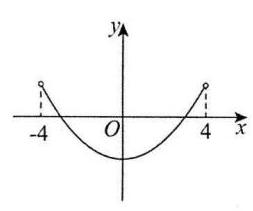
\includegraphics[max width=0.2\textwidth]{images/bo_d5jma53ef24c73bll4ig_19_1204_1357_253_211_0.jpg}
\end{center}
\hspace*{3em} 

【练习】9. (2025 届复附) 函数 \(y = f\left( x\right)\) 是定义在 \(\left( {-4,4}\right)\) 上的偶函数，其图像如图所示，满足 \(f\left( 3\right)  = 0\) ，设 \({y}^{\prime } = {f}^{\prime }\left( x\right)\) 是 \(y = f\left( x\right)\) 的导函数，则关于 \(x\) 的不等式 \(f\left( {x + 1}\right)  \cdot  {f}^{\prime }\left( x\right)  \geq  0\) 的解集是\_\_\_\_\_

【答案】 \(\left( {-4,0\rbrack \cup \lbrack 2,3}\right)\)

【解析】函数 \(y = f\left( x\right)\) 是偶函数,所以 \(f\left( {-3}\right)  = f\left( 3\right)  = 0\) ,

当 \(x \in  \left\lbrack  {-3,3}\right\rbrack\) 时, \(f\left( x\right)  \leq  0\) ,所以 \(x \in  \left\lbrack  {-4,2}\right\rbrack\) 时, \(f\left( {x + 1}\right)  \leq  0\) ,

当 \(x \in  ( - 4, - 3\rbrack  \cup  \lbrack 3,4)\) 时, \(f\left( x\right)  \geq  0\) ,所以 \(x \in  ( - 5, - 4\rbrack  \cup  \lbrack 2,3)\) 时, \(f\left( {x + 1}\right)  \geq  0\) ,

当 \(x \in  ( - 4,0\rbrack\) 时, \({f}^{\prime }\left( x\right)  \leq  0\) ; 当 \(x \in  \lbrack 0,4)\) 时, \({f}^{\prime }\left( x\right)  \geq  0\) ,

因为 \(f\left( {x + 1}\right)  \cdot  {f}^{\prime }\left( x\right)  \geq  0\) ,所以 \(\left\{  \begin{array}{l} f\left( {x + 1}\right)  \geq  0 \\  {f}^{\prime }\left( x\right)  \geq  0 \end{array}\right.\) 或 \(\left\{  \begin{array}{l} f\left( {x + 1}\right)  \leq  0 \\  {f}^{\prime }\left( x\right)  \leq  0 \end{array}\right.\) ,

即 \(\left\{  \begin{array}{l} x \in  ( - 5, - 4\rbrack  \cup  \lbrack 2,3) \\  x \in  \lbrack 0,4) \end{array}\right.\) 或 \(\left\{  \begin{array}{l} x \in  \left\lbrack  {-4,2}\right\rbrack  \\  x \in  ( - 4,0\rbrack  \end{array}\right.\) ,所以 \(x \in  \left\lbrack  {2,3)\text{ 或 }x \in  ( - 4,0}\right\rbrack\)

故解集为 \(\left( {-4,0\rbrack \cup \lbrack 2,3}\right)\)

【练习】10. (2024 届格致) 设函数 \(f\left( x\right)  = \frac{{ax} + b}{{x}^{2} - c}(a,b,c\) 为常数) 的部分图像如右图所示,则 \(a + b + c =\) \_\_\_\_\_.

\begin{center}
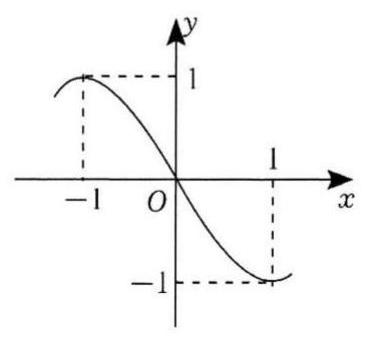
\includegraphics[max width=0.3\textwidth]{images/bo_d5jma53ef24c73bll4ig_20_1093_242_366_338_0.jpg}
\end{center}
\hspace*{3em} 

【答案】-3

【解析】由题意得 \(f\left( x\right)\) 的定义域为 \(R\) ,所以 \(c < 0\) ,且 \(f\left( 0\right)  = 0\) ,

故有 \(f\left( 0\right)  = \frac{b}{-c} = 0 \Rightarrow  b = 0\) ,则 \(f\left( x\right)  = \frac{ax}{{x}^{2} - c}\) ,

因为 \(f\left( 1\right)  =  - 1\) ,有 \(\frac{a}{1 - c} =  - 1 \Rightarrow  a = c - 1 \Rightarrow  c = a + 1\) ,

由于 \(f\left( x\right)\) 在 \(\left\lbrack  {-1,1}\right\rbrack\) 上严格减，在 \(\left( {-\infty , - 1\rbrack \text{ 和 }\lbrack 1, + \infty }\right)\) 上严格增,

故有 \({f}^{\prime }\left( {-1}\right)  = {f}^{\prime }\left( 1\right)  = 0\) ,而 \(f\left( x\right)  = \frac{ax}{{x}^{2} - c}\) ,

所以 \({f}^{\prime }\left( x\right)  = \frac{a\left( {{x}^{2} - c}\right)  - {ax} \cdot  {2x}}{{\left( {x}^{2} - c\right) }^{2}} = \frac{-a{x}^{2} - {ac}}{{\left( {x}^{2} - c\right) }^{2}}\) ,

代入 \({f}^{\prime }\left( 1\right)  = \frac{-a - {ac}}{{\left( 1 - c\right) }^{2}} = 0 \Rightarrow   - a - {ac} = 0 \Rightarrow  c + 1 = 0 \Rightarrow  c =  - 1\) ,

则 \(a =  - 2\) ,故 \(a + b + c =  - 2 + 0 - 1 =  - 3\) .

\section*{板块二: 中档客观题}

\section*{1. 真题回顾}

A、旋转后仍是函数

【例题】1. (2018 上海秋考) 设 \(D\) 是含数 1 的有限实数集, \(f\left( x\right)\) 是定义在 \(D\) 上的函数,若 \(f\left( x\right)\) 的图象绕原点逆时针旋转 \(\frac{\pi }{6}\) 后与原图象重合,则在以下各项中, \(f\left( 1\right)\) 的可能取值只能是 ( )

A. \(\sqrt{3}\) B. \(\frac{\sqrt{3}}{2}\) C. \(\frac{\sqrt{3}}{3}\) D. 0

【答案】 \(B\)

【解析】问题相当于圆上由 12 个点为一组,每次绕原点逆时针旋转 \(\frac{\pi }{6}\) 个单位后与下一个点会重合. 我们可以通过代入和赋值的方法,当 \(f\left( 1\right)  = \sqrt{3}\text{ 、 }\frac{\sqrt{3}}{3}\text{ 、 }0\) 时, 此时得到的圆心角为 \(\frac{\pi }{3}\text{ 、 }\frac{\pi }{6}\text{ 、 }0\) ,然而此时 \(x = 0\) 或者 \(x = 1\) 时, 都有 2 个 \(y\) 与之对应,而我们知道函数的定义就是要求一个 \(x\) 只能对应一个 \(y\) , 因此只有当 \(x = \frac{\sqrt{3}}{2}\) ，此时旋转 \(\frac{\pi }{6}\) ，此时满足一个 \(x\) 只会对应一个 \(y\) ，故选 \(B\) .

【例题】2. (2009 上海秋考) 将函数 \(y = \sqrt{4 + {6x} - {x}^{2}} - 2\left( {x \in  \left\lbrack  {0,6}\right\rbrack  }\right)\) 的图象绕坐标原点逆时针方向旋转角 \(\theta \left( {0 \leq  \theta  \leq  \alpha }\right)\) ,得到曲线 \(C\) . 若对于每一个旋转角 \(\theta\) ,曲线 \(C\) 都是一个函数的图象,则 \(\alpha\) 的最大值为\_\_\_\_\_.

【答案】 \(\arctan \frac{2}{3}\)

\begin{center}
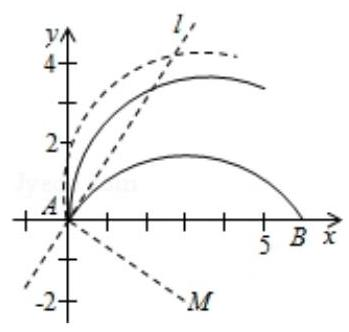
\includegraphics[max width=0.2\textwidth]{images/bo_d5jma53ef24c73bll4ig_21_1110_1193_349_332_0.jpg}
\end{center}
\hspace*{3em} 

【解析】先画出函数 \(y = \sqrt{4 + {6x} - {x}^{2}} - 2\left( {x \in  \left\lbrack  {0,6}\right\rbrack  }\right)\) 的图象,

这是一个圆弧,圆心为 \(M\left( {3, - 2}\right)\) ,

由图像得当此圆弧绕坐标原点逆时针方向旋转角大于 \(\angle {MAB}\) 时, 曲线 \(C\) 都不是一个函数的图象, \(\angle {MAB} = \arctan \frac{2}{3}\) ,

故 \(\alpha\) 的最大值为 \(\arctan \frac{2}{3}\) .

B、综合

【例题】1. (2021 上海春考) 已知函数 \(y = f\left( x\right)\) 的定义域为 \(R\) ,下列是 \(f\left( x\right)\) 无最大值的充分条件是 ( )

A. \(f\left( x\right)\) 为偶函数且关于点 \(\left( {1,1}\right)\) 对称 B. \(f\left( x\right)\) 为偶函数且关于直线 \(x = 1\) 对称

C. \(f\left( x\right)\) 为奇函数且关于点 \(\left( {1,1}\right)\) 对称 D. \(f\left( x\right)\) 为奇函数且关于直线 \(x = 1\) 对称

【答案】 \(C\)

【解析】对于 \(A,f\left( x\right)  = \cos \frac{\pi x}{2} + 1,f\left( x\right)\) 为偶函数,且关于点 \(\left( {1,1}\right)\) 对称,存在最大值, \(A\) 错误,

对于 \(B,f\left( x\right)  = \cos \left( {\pi x}\right) ,f\left( x\right)\) 为偶函数且关于直线 \(x = 1\) 对称,存在最大值, \(B\) 错误,

对于 \(C\) ,假设 \(f\left( x\right)\) 有最大值,设其最大值为 \(M\) ,其最高点的坐标为 \(\left( {a,M}\right)\) ,

\(f\left( x\right)\) 为奇函数，其图象关于原点对称，则 \(f\left( x\right)\) 的图象存在最低点 \(\left( {-a, - M}\right)\) ，

又由 \(f\left( x\right)\) 的图象关于点 \(\left( {1,1}\right)\) 对称,

则 \(\left( {-a, - M}\right)\) 关于点 \(\left( {1,1}\right)\) 对称的点为 \(\left( {2 + a,2 + M}\right)\) ,

与最大值为 \(M\) 相矛盾，则此时 \(f\left( x\right)\) 无最大值， \(C\) 正确，

对于 \(D,f\left( x\right)  = \sin \frac{\pi x}{2},f\left( x\right)\) 为奇函数且关于直线 \(x = 1\) 对称， \(D\) 错误，

故选 \(C\) .

【例题】2. (2020 上海秋考) 设 \(a \in  R\) ，若存在定义域为 \(R\) 的函数 \(f\left( x\right)\) 同时满足下列两个条件:

(1) 对任意的 \({x}_{0} \in  R,f\left( {x}_{0}\right)\) 的值为 \({x}_{0}\) 或 \({x}_{0}^{2}\) ;

( 2 )关于 \(x\) 的方程 \(f\left( x\right)  = a\) 无实数解，则 \(a\) 的取值范围是\_\_\_\_\_.

【答案】 \(\left( {-\infty ,0}\right)  \cup  \left( {0,1}\right)  \cup  \left( {1, + \infty }\right)\)

【解析】由 (1) 得 \(f\left( 0\right)  = 0\) 且 \(f\left( 1\right)  = 1\) ,

又因为关于 \(x\) 的方程 \(f\left( x\right)  = a\) 无实数解,所以 \(a \neq  0\) 且 \(a \neq  1\) ,

此时存在函数 \(f\left( x\right)  = \left\{  \begin{array}{l} {x}^{2},x = a \\  x,x \neq  a \end{array}\right.\) 满足题意,所以 \(a \in  \left( {-\infty ,0}\right)  \cup  \left( {0,1}\right)  \cup  \left( {1, + \infty }\right)\) .

【例题】3. (2020 上海秋考) 命题 \(p\) : 存在 \(a \in  R\) 且 \(a \neq  0\) ,对于任意的 \(x \in  R\) ,使得 \(f\left( {x + a}\right)  < f\left( x\right)  + \; f\left( a\right)\) ;

命题 \({q}_{1} : f\left( x\right)\) 严格单调递减且 \(f\left( x\right)  > 0\) 恒成立;

命题 \({q}_{2} : f\left( x\right)\) 严格单调递增,存在 \({x}_{0} < 0\) 使得 \(f\left( {x}_{0}\right)  = 0\) ,

则下列说法正确的是 ( )

A. 只有 \({q}_{1}\) 是 \(p\) 的充分条件 B. 只有 \({q}_{2}\) 是 \(p\) 的充分条件

C. \({q}_{1}\text{ 、 }{q}_{2}\) 都是 \(p\) 的充分条件 D. \({q}_{1}\text{ 、 }{q}_{2}\) 都不是 \(p\) 的充分条件

【答案】 \(C\)

【解析】对于命题 \({q}_{1}\) : 当 \(f\left( x\right)\) 严格单调递减且 \(f\left( x\right)  > 0\) 恒成立时,

当 \(a > 0\) 时,此时 \(x + a > x\) ,又因为 \(f\left( x\right)\) 严格单调递减,所以 \(f\left( {x + a}\right)  < f\left( x\right)\)

又因为 \(f\left( x\right)  > 0\) 恒成立，所以 \(f\left( x\right)  < f\left( x\right)  + f\left( a\right)\) ，所以 \(f\left( {x + a}\right)  < f\left( x\right)  + f\left( a\right)\) ，

所以命题 \({q}_{1} \Rightarrow\) 命题 \(p\) ,

对于命题 \({q}_{2} :\) 当 \(f\left( x\right)\) 严格单调递增,存在 \({x}_{0} < 0\) 使得 \(f\left( {x}_{0}\right)  = 0\) ,

当 \(a = {x}_{0} < 0\) 时,此时 \(x + a < x,f\left( a\right)  = f\left( {x}_{0}\right)  = 0\) ,

又因为 \(f\left( x\right)\) 严格单调递增,所以 \(f\left( {x + a}\right)  < f\left( x\right)\) ,所以 \(f\left( {x + a}\right)  < f\left( x\right)  + f\left( a\right)\) , 所以命题 \({p}_{2} \Rightarrow\) 命题 \(p\) ,

所以 \({q}_{1}\text{ 、 }{q}_{2}\) 都是 \(p\) 的充分条件,故选 \(C\) .

\begin{center}
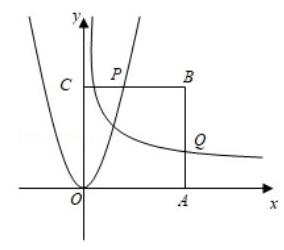
\includegraphics[max width=0.2\textwidth]{images/bo_d5jma53ef24c73bll4ig_22_1170_1661_284_250_0.jpg}
\end{center}
\hspace*{3em} 

【例题】4. (2019 上海春考) 如图,已知正方形 \({OABC}\) ,其中 \({OA} = a\left( {a > 1}\right)\) ,函数 \(y = 3{x}^{2}\) 交 \({BC}\) 于点 \(P\) ，函数 \(y = {x}^{-\frac{1}{2}}\) 交 \({AB}\) 于点 \(Q\) ，当 \(\left| {AQ}\right|  + \left| {CP}\right|\) 最小时，则 \(a\) 的值为\_\_\_\_\_.

【答案】 \(\sqrt{3}\)

【解析】由题意得 \(P\) 点坐标为 \(\left( {\sqrt{\frac{a}{3}},a}\right) ,Q\) 点坐标为 \(\left( {a,\sqrt{\frac{1}{a}}}\right)\) ,

\(\left| {AQ}\right|  + \left| {CP}\right|  = \sqrt{\frac{a}{3}} + \sqrt{\frac{1}{a}} \geq  2\sqrt{\frac{1}{\sqrt{3}}},\)

当且仅当 \(a = \sqrt{3}\) 时，取最小值.

【例题】5. (2018 上海秋考) 已知常数 \(a > 0\) ，函数 \(f\left( x\right)  = \frac{{2}^{x}}{{2}^{x} + {ax}}\) 的图象经过点 \(P\left( {p,\frac{6}{5}}\right)\) ， \(Q\left( {q, - \frac{1}{5}}\right)\) .

若 \({2}^{p + q} = {36pq}\) ,则 \(a =\) \_\_\_\_\_.

【答案】 6

【解析】函数 \(f\left( x\right)  = \frac{{2}^{x}}{{2}^{x} + {ax}}\) 的图象经过点 \(P\left( {p,\frac{6}{5}}\right) ,Q\left( {q, - \frac{1}{5}}\right)\) .

法一: \(\frac{{2}^{p}}{{2}^{p} + {ap}} + \frac{{2}^{q}}{{2}^{q} + {aq}} = \frac{6}{5} - \frac{1}{5} = 1\) ,整理得 \(\frac{{2}^{p + q} + {2}^{p}{aq} + {2}^{q}{ap} + {2}^{p + q}}{{2}^{p + q} + {2}^{p}{aq} + {2}^{q}{ap} + {a}^{2}{pq}} = 1\) ,

解得 \({2}^{p + q} = {a}^{2}{pq}\) ,由于 \({2}^{p + q} = {36pq}\) ,所以 \({a}^{2} = {36}\) ,

由于 \(a > 0\) ，故 \(a = 6\) .

法二: \(\frac{{2}^{p}}{{2}^{p} + {ap}} = \frac{6}{5} \Rightarrow  \frac{1}{1 + \frac{ap}{{2}^{p}}} = \frac{6}{5}\) ,所以 \(\frac{ap}{{2}^{p}} =  - \frac{1}{6}\) ,

\(\frac{{2}^{q}}{{2}^{q} + {aq}} =  - \frac{1}{5} \Rightarrow  \frac{1}{1 + \frac{aq}{{2}^{q}}} =  - \frac{1}{5}\) ,所以 \(\frac{aq}{{2}^{q}} =  - 6\) ,

两式相乘得 \(\frac{{a}^{2}{pq}}{{2}^{p + q}} = 1\) ,因为 \({2}^{p + q} = {36pq}\) ,所以 \(\frac{{a}^{2}}{36} = 1\) ,由于 \(a > 0\) ,故 \(a = 6\) .

【例题】6. (2017 上海春考) 设 \(a,b \in  R\) ,若函数 \(f\left( x\right)  = x + \frac{a}{x} + b\) 在区间 \(\left( {1,2}\right)\) 上有两个不同的零点, 则 \(f\left( 1\right)\) 的取值范围为\_\_\_\_\_.

【答案】 \(\left( {0,1}\right)\)

\begin{center}
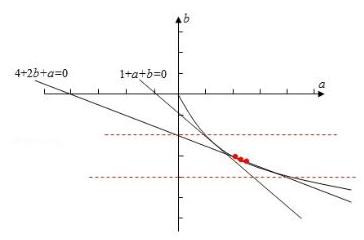
\includegraphics[max width=0.3\textwidth]{images/bo_d5jma53ef24c73bll4ig_23_1093_1035_364_240_0.jpg}
\end{center}
\hspace*{3em} 

【解析】法一: 函数 \(f\left( x\right)  = x + \frac{a}{x} + b\) 在区间 \(\left( {1,2}\right)\) 上有两个不同的零点, 即方程 \({x}^{2} + {bx} + a = 0\) 在区间 \(\left( {1,2}\right)\) 上两个不相等的实根，

\(\Rightarrow  \left\{  {\begin{array}{l} 1 <  - \frac{b}{2} < 2 \\  {b}^{2} - {4a} > 0 \\  1 + a + b > 0 \\  4 + {2b} + a > 0 \end{array} \Rightarrow  \left\{  \begin{array}{l}  - 4 < b <  - 2 \\  {b}^{2} > {4a} \\  1 + a + b > 0 \\  4 + {2b} + a > 0 \end{array}\right. }\right.\) ,

如图画出数对 \(\left( {a,b}\right)\) 所表示的区域,目标函数 \(z = f\left( a\right)  = a + b + 1\) ,

所以 \(z\) 的最小值为 \(z = a + b + 1\) 过点 \(\left( {1, - 2}\right)\) 时,

\(z\) 的最大值为 \(z = a + b + 1\) 过点 \(\left( {4, - 4}\right)\) 时,

所以 \(f\left( 1\right)\) 的取值范围为 \(\left( {0,1}\right)\) .

法二: 函数 \(f\left( x\right)  = x + \frac{a}{x} + b\) 在区间 \(\left( {1,2}\right)\) 上有两个不同的零点,

即方程 \({x}^{2} + {bx} + a = 0\) 在区间 \(\left( {1,2}\right)\) 上两个不相等的实根，设为 \({x}_{1},{x}_{2}\left( {{x}_{1} \neq  {x}_{2}}\right)\) ，

则 \({x}_{1} + {x}_{2} =  - b,{x}_{1}{x}_{2} = a\) ,

所以 \(f\left( 1\right)  = a + b + 1 = {x}_{1}{x}_{2} - \left( {{x}_{1} + {x}_{2}}\right)  + 1 = \left( {{x}_{1} - 1}\right) \left( {{x}_{2} - 1}\right)\) ,

因为 \({x}_{1},{x}_{2} \in  \left( {1,2}\right) ,{x}_{1} \neq  {x}_{2}\) ,所以 \(f\left( 1\right)  \in  \left( {0,1}\right)\) .

【例题】7. (2016 上海秋考) 设 \(f\left( x\right) \text{ 、 }g\left( x\right) \text{ 、 }h\left( x\right)\) 是定义域为 \(R\) 的三个函数，对于命题: \circled{1}  \(f\left( x\right)  + g\left( x\right)\) 、 \(f\left( x\right)  + h\left( x\right) \text{ 、 }g\left( x\right)  + h\left( x\right)\) 均为严格增函数,则 \(f\left( x\right) \text{ 、 }g\left( x\right) \text{ 、 }h\left( x\right)\) 中至少有一个严格增函数;  \circled{2} 若 \(f\left( x\right)  + g\left( x\right) \text{ 、 }f\left( x\right)  + h\left( x\right) \text{ 、 }g\left( x\right)  + h\left( x\right)\) 均是以 \(T\) 为周期的函数,则 \(f\left( x\right) \text{ 、 }g\left( x\right) \text{ 、 }h\left( x\right)\) 均是以 \(T\) 为周期的函数，下列判断正确的是 ( )

A.  \circled{1} 和 \circled{2} 均为真命题 B.  \circled{1} 和 \circled{2} 均为假命题

C.  \circled{1} 为真命题， \circled{2} 为假命题 D.  \circled{1} 为假命题， \circled{2} 为真命题

【答案】 \(D\)

【解析】 \circled{1}  不成立. 可举反例: \(f\left( x\right)  = \left\{  {\begin{array}{ll} {2x}, & x \leq  1 \\   - x + 3, & x > 1 \end{array}.g\left( x\right)  = \left\{  \begin{array}{ll} {2x} + 3, & x \leq  0 \\   - x + 3, & 0 < x < 1, \\  {2x}, & x \geq  1 \end{array}\right. }\right.\)

\(h\left( x\right)  = \left\{  {\begin{array}{ll}  - x, & x \leq  0 \\  {2x}, & x > 0 \end{array}.}\right.\)

 \circled{2} 因为 \(f\left( x\right)  + g\left( x\right)  = f\left( {x + T}\right)  + g\left( {x + T}\right) ,f\left( x\right)  + h\left( x\right)  = f\left( {x + T}\right)  + h\left( {x + T}\right)\) ，

\(h\left( x\right)  + g\left( x\right)  = h\left( {x + T}\right)  + g\left( {x + T}\right) ,\)

前两式作差得 \(g\left( x\right)  - h\left( x\right)  = g\left( {x + T}\right)  - h\left( {x + T}\right)\) ,

结合第三式得 \(g\left( x\right)  = g\left( {x + T}\right) ,h\left( x\right)  = h\left( {x + T}\right)\) ,同理可得 \(f\left( x\right)  = f\left( {x + T}\right)\) ,

因此 \circled{2} 正确. 故选 \(D\) .

\begin{center}
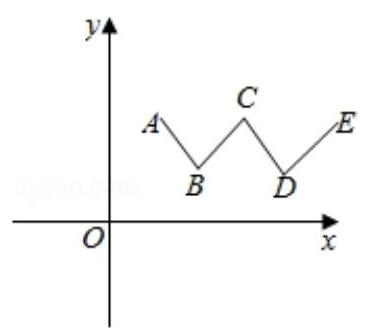
\includegraphics[max width=0.3\textwidth]{images/bo_d5jma53ef24c73bll4ig_24_1092_744_365_334_0.jpg}
\end{center}
\hspace*{3em} 

【例题】8. (2016 上海春考) 已知函数 \(y = f\left( x\right)\) 的图象是折线 \({ABCDE}\) ,如图,其中 \(A\left( {1,2}\right) ,B\left( {2,1}\right) ,C\left( {3,2}\right) ,D\left( {4,1}\right) ,E\left( {5,2}\right)\) ,若直线 \(y = {kx} \; + b\) 与 \(y = f\left( x\right)\) 的图象恰有四个不同的公共点,则 \(k\) 的取值范围是 ( )

A. \(\left( {-1,0}\right)  \cup  \left( {0,1}\right)\) B. \(\left( {-\frac{1}{3},\frac{1}{3}}\right)\)

C. \((0,1\rbrack\) D. \(\left\lbrack  {0.\frac{1}{3}}\right\rbrack\)

【答案】 \(B\)

\begin{center}
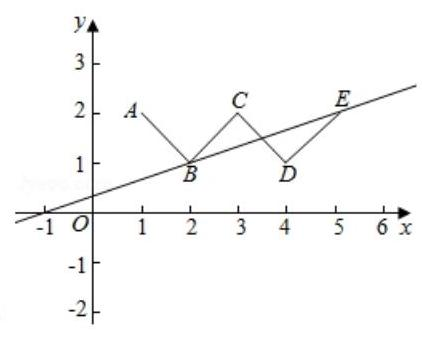
\includegraphics[max width=0.3\textwidth]{images/bo_d5jma53ef24c73bll4ig_24_1034_1087_422_339_0.jpg}
\end{center}
\hspace*{3em} 

【解析】当 \(k = 0,1 < b < 2\) 时,显然直线 \(y = b\) 与 \(f\left( x\right)\) 图象交于四点,故 \(k\) 可以取 0,

排除 \(A,C\)

作直线 \({BE}\) ,则 \({k}_{BE} = \frac{2 - 1}{5 - 2} = \frac{1}{3}\) ,直线 \({BE}\) 与 \(f\left( x\right)\) 图象交于三点,

平行移动直线 \({BD}\) 可发现直线与 \(f\left( x\right)\) 图象最多交于三点, 即直线 \(y = \frac{1}{3}x + b\) 与 \(f\left( x\right)\) 图象最多交于三点,所以 \(k \neq  \frac{1}{3}\) . 排除 \(D\) .

故选 \(B\) .

【例题】9. (2015 上海秋考) 已知函数 \(f\left( x\right)  = \sin x\) . 若存在 \({x}_{1},{x}_{2},\cdots ,{x}_{m}\) 满足 \(0 \leq  {x}_{1} < {x}_{2} < \cdots  < {x}_{m} \leq \; {6\pi }\) ,且 \(\left| {f\left( {x}_{1}\right)  - f\left( {x}_{2}\right) }\right|  + \left| {f\left( {x}_{2}\right)  - f\left( {x}_{3}\right) }\right|  + \cdots  + \left| {f\left( {x}_{m - 1}\right)  - f\left( {x}_{m}\right) }\right|  = {12}\left( {m \geq  2,m \in  {N}^{ * }}\right)\) ,则 \(m\) 的最小值为\_\_\_\_\_.

【答案】 8

【解析】因为 \(y = \sin x\) 对任意 \({x}_{i},{x}_{j}\left( {\mathrm{i},j = 1,2,3,\cdots ,m}\right)\) ,

都有 \(\left| {f\left( {x}_{i}\right)  - f\left( {x}_{j}\right) }\right|  \leq  f{\left( x\right) }_{\max } - f{\left( x\right) }_{\min } = 2\) ,

要使 \(m\) 取得最小值,尽可能多让 \({x}_{i}\left( {\mathrm{i} = 1,2,3,\cdots ,m}\right)\) 取得最高点,

考虑 \(0 \leq  {x}_{1} < {x}_{2} < \cdots  < {x}_{m} \leq  {6\pi }\) ,

\(\left| {f\left( {x}_{1}\right)  - f\left( {x}_{2}\right) }\right|  + \left| {f\left( {x}_{2}\right)  - f\left( {x}_{3}\right) }\right|  + \cdots  + \left| {f\left( {x}_{m - 1}\right)  - f\left( {x}_{m}\right) }\right|  = {12},\)

按下图取值即可满足条件，所以 \(m\) 的最小值为 8 .

\begin{center}
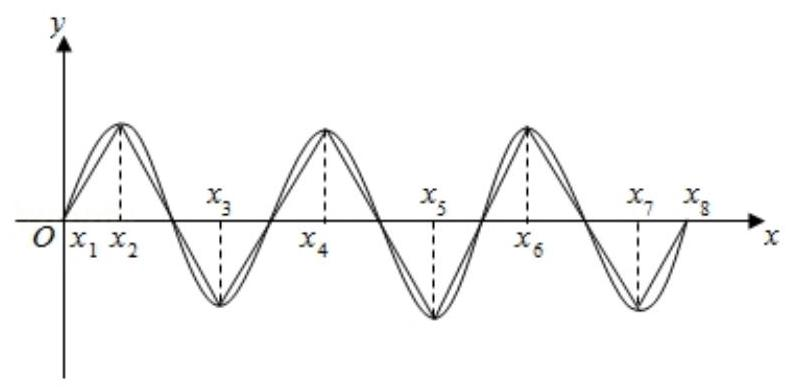
\includegraphics[max width=0.6\textwidth]{images/bo_d5jma53ef24c73bll4ig_25_294_231_791_388_0.jpg}
\end{center}
\hspace*{3em} 

【例题】10. (2012 上海秋考) 已知函数 \(y = f\left( x\right)\) 的图象是折线段 \({ABC}\) ,其中 \(A\left( {0,0}\right) \text{ 、 }B\left( {\frac{1}{2},5}\right) \text{ 、 }C\left( {1,0}\right)\) , 函数 \(y = {xf}\left( x\right) \left( {0 \leq  x \leq  1}\right)\) 的图象与 \(x\) 轴围成的图形的面积为\_\_\_\_\_.

【答案】 \(\frac{5}{4}\)

【解析】由题意得 \(f\left( x\right)  = \left\{  \begin{array}{ll} {10x}, & \left( {0 \leq  x \leq  \frac{1}{2}}\right) \\  {10} - {10x}, & \left( {\frac{1}{2} \leq  x \leq  1}\right)  \end{array}\right.\) ,所以 \(y = {xf}\left( x\right)  = \left\{  \begin{array}{ll} {10}{x}^{2}, & \left( {0 \leq  x \leq  \frac{1}{2}}\right) \\   - {10}{x}^{2} + {10x}, & \left( {\frac{1}{2} \leq  x \leq  1}\right)  \end{array}\right.\) , 设函数 \(y = {xf}\left( x\right) \left( {0 \leq  x \leq  1}\right)\) 的图象与 \(x\) 轴围成的图形的面积为 \(S\) , 则 \(S = {\int }_{0}^{\frac{1}{2}}{10}{x}^{2}\mathrm{\;d}x + {\int }_{\frac{1}{2}}^{1}\left( {-{10}{x}^{2} + {10x}}\right) \mathrm{d}x = {\left. {10} \times  \frac{{x}^{3}}{3}\right| }_{0}^{\frac{1}{2}} + {\left. \left( -{10}\right)  \times  \frac{{x}^{3}}{3}\right| }_{\frac{1}{2}}^{1} + {\left. {10} \times  \frac{{x}^{2}}{2}\right| }_{\frac{1}{2}}^{1} \; = \frac{5}{12} - \frac{35}{12} + 5 - \frac{5}{4} = \frac{15}{12} = \frac{5}{4}\) .

【注】本题也可以用割补的方法求解.

\section*{2. 模拟练习}

注:有些是介于 15 和 16 之间的难度, 不少题来自 2025 版每日三题

【练习】1. (2025 届复附) 设集合 \(P = \{  - 1,1\} ,Q = \{ x \mid  x > 0\) 且 \(x \neq  1\}\) ,函数 \(f\left( x\right)  = {a}^{x} + \; \lambda {a}^{-x}\left( {a > 0\text{ 且 }a \neq  1}\right)\) ，下列四个命题:

 \circled{1} 对任意 \(\lambda  \in  P\) ，存在 \(a \in  Q\) ，使得 \(y = f\left( x\right)\) 是增函数；

 \circled{2}  存在 \(\lambda  \in  P\) ，对任意 \(a \in  Q\) ， \(y = f\left( x\right)\) 是减函数；

 \circled{3} 对任意 \(\lambda  \in  P\) ，存在 \(a \in  Q\) ，使得 \(y = f\left( x\right)\) 是奇函数；

 \circled{4}  存在 \(\lambda  \in  P\) ，对任意 \(a \in  Q\) ， \(y = f\left( x\right)\) 是偶函数

其中真命题的个数是 ( )

A. 1 个 B. 2 个 C. 3 个 D. 4 个

【答案】 \(A\)

【解析】 \(< 1 >\) 当 \(\lambda  = 1,a \in  \left( {0,1}\right)\) 时, \(f\left( x\right)  = {a}^{x} + {a}^{-x}\) ,

则 \({f}^{\prime }\left( x\right)  = {a}^{x}\ln a - {a}^{-x}\ln a = \ln a\left( {{a}^{x} - {a}^{-x}}\right)\) ,因为 \(a \in  \left( {0,1}\right)\) ,所以 \(\ln a < 0\) ,

所以当 \(x \in  \left( {-\infty ,0}\right)\) 时, \({a}^{x} - {a}^{-x} > 0\) ,即 \({f}^{\prime }\left( x\right)  < 0\) ;

当 \(x \in  \left( {0, + \infty }\right)\) 时, \({a}^{x} - {a}^{-x} < 0\) ,即 \({f}^{\prime }\left( x\right)  > 0\) ,

所以 \(f\left( x\right)\) 严格减区间为 \(\left( {-\infty ,0}\right)\) ,严格增区间为 \(\left( {0, + \infty }\right)\)

因为 \(f\left( {-x}\right)  = {a}^{-x} + {a}^{x} = f\left( x\right)\) ，所以 \(f\left( x\right)\) 为偶函数

\(< 2 >\) 当 \(\lambda  = 1,a \in  \left( {1, + \infty }\right)\) 时, \(f\left( x\right)  = {a}^{x} + {a}^{-x}\) ,

则 \({f}^{\prime }\left( x\right)  = {a}^{x}\ln a - {a}^{-x}\ln a = \ln a\left( {{a}^{x} - {a}^{-x}}\right)\) ,因为 \(a \in  \left( {1, + \infty }\right)\) ,所以 \(\ln a > 0\) ,

所以当 \(x \in  \left( {-\infty ,0}\right)\) 时, \({a}^{x} - {a}^{-x} < 0\) ,即 \({f}^{\prime }\left( x\right)  < 0\) ;

当 \(x \in  \left( {0, + \infty }\right)\) 时, \({a}^{x} - {a}^{-x} > 0\) ,即 \({f}^{\prime }\left( x\right)  > 0\) ,

所以 \(f\left( x\right)\) 严格减区间为 \(\left( {-\infty ,0}\right)\) ,严格增区间为 \(\left( {0, + \infty }\right)\)

因为 \(f\left( {-x}\right)  = {a}^{-x} + {a}^{x} = f\left( x\right)\) ,所以 \(f\left( x\right)\) 为偶函数

\(< 3 >\) 当 \(\lambda  =  - 1,a \in  \left( {0,1}\right)\) 时, \(f\left( x\right)  = {a}^{x} - {a}^{-x}\) ,

则 \({f}^{\prime }\left( x\right)  = {a}^{x}\ln a + {a}^{-x}\ln a = \ln a\left( {{a}^{x} + {a}^{-x}}\right)\) ,因为 \(a \in  \left( {0,1}\right)\) ,所以 \(\ln a < 0\) ,

又因为 \({a}^{x} + {a}^{-x} > 0\) 恒成立,所以 \({f}^{\prime }\left( x\right)  < 0\) 恒成立,所以 \(f\left( x\right)\) 是减函数

因为 \(f\left( {-x}\right)  = {a}^{-x} - {a}^{x} =  - f\left( x\right)\) ,所以 \(f\left( x\right)\) 为奇函数

\(< 4 >\) 当 \(\lambda  =  - 1,a \in  \left( {1, + \infty }\right)\) 时, \(f\left( x\right)  = {a}^{x} - {a}^{-x}\) ,

则 \({f}^{\prime }\left( x\right)  = {a}^{x}\ln a + {a}^{-x}\ln a = \ln a\left( {{a}^{x} + {a}^{-x}}\right)\) ,因为 \(a \in  \left( {1, + \infty }\right)\) ,所以 \(\ln a > 0\) ,

又因为 \({a}^{x} + {a}^{-x} > 0\) 恒成立，所以 \({f}^{\prime }\left( x\right)  > 0\) 恒成立，

所以 \(f\left( x\right)  = {a}^{x} - {a}^{-x}\) 是增函数

因为 \(f\left( {-x}\right)  = {a}^{-x} - {a}^{x} =  - f\left( x\right)\) ,所以 \(f\left( x\right)\) 为奇函数

综上,对于 \circled{1} ,由上述 \(\langle 1\rangle ,\langle 2\rangle\) 得,当 \(\lambda  = 1,\forall a \in  Q\) 时, \(y = f\left( x\right)\) 不是增函数, 故 \circled{1} 不正确；

对于 \circled{2} ，由上述 \(< 1 > , < 2 >\) 得，当 \(\lambda  = 1\) ， \(\forall a \in  Q\) 时， \(y = f\left( x\right)\) 不是减函数，

由上述 \(\langle 3\rangle ,\langle 4\rangle\) 得,当 \(\lambda  =  - 1,a \in  \left( {1, + \infty }\right)\) 时, \(f\left( x\right)\) 是增函数，故 \circled{2} 不正确；

对于 \circled{3} ，由上述 \(\langle 1\rangle\) ， \(\langle 2\rangle\) 得，当 \(\lambda  = 1\) ， \(\forall a \in  Q\) 时， \(y = f\left( x\right)\) 是偶函数，

故 \circled{3} 不正确；

对于 \circled{4} ，由上述 \(\langle 3\rangle ,\langle 4\rangle\) 得，当 \(\lambda  =  - 1\) ， \(\forall a \in  Q\) 时， \(y = f\left( x\right)\) 是奇函数，

故 \circled{4} 正确

故选 \(A\)

【练习】2. 已知 \(a > 0\) ,过点 \(\left( {a,b}\right)\) 可以作曲线 \(y = {x}^{3}\) 的三条切线,则下列说法正确的有\_\_\_\_\_

 \circled{1}  \(b < 0\)  \circled{2}  \(b > 0\)  \circled{3}  \(b < {a}^{3}\)  \circled{4}  \(b > {a}^{3}\)

【答案】 \circled{2}  \circled{3} 

【解析】设切点为 \(\left( {{x}_{0},{x}_{0}^{3}}\right)\) ,

因为 \({y}^{\prime } = 3{x}^{2}\) ,即 \({\left. {y}^{\prime }\right| }_{x = {x}_{0}} = 3{x}_{0}^{2}\) ,

切线方程为 \(y - {x}_{0}^{3} = 3{x}_{0}^{2}\left( {x - {x}_{0}}\right)\) ,

所以 \(b - {x}_{0}^{3} = 3{x}_{0}^{2}\left( {a - {x}_{0}}\right)\) ,即 \(b =  - 2{x}_{0}^{3} + {3a}{x}_{0}^{2}\) ,

因为过点 \(\left( {a,b}\right)\) 可以作曲线 \(y = {x}^{3}\) 的三条切线,

所以,关于 \({x}_{0}\) 的方程 \(b =  - 2{x}_{0}^{3} + {3a}{x}_{0}^{2}\) 有三个不同的解.

设 \(f\left( x\right)  =  - 2{x}^{3} + {3a}{x}^{2}\) ,则 \({f}^{\prime }\left( x\right)  =  - 6{x}^{2} + {6ax} =  - {6x}\left( {x - a}\right)\) ,

所以 \(f\left( x\right)\) 在 \(\left( {0,a}\right)\) 上单调递增,在 \(\left( {-\infty ,0}\right)\) 和 \(\left( {a, + \infty }\right)\) 上单调递减,且值域为 \(R\) ,

所以 \(\left\{  \begin{array}{l} b > f\left( 0\right) \\  b < f\left( a\right)  \end{array}\right.\) ,即 \(\left\{  \begin{array}{l} b > 0 \\  b < {a}^{3} \end{array}\right.\) .

故选: \circled{2}  \circled{3} 

【练习】3. 设曲线 \(C\) 与函数 \(f\left( x\right)  = \frac{\sqrt{3}}{12}{x}^{2}\left( {0 \leq  x \leq  m}\right)\) 的图像关于直线 \(y = \sqrt{3}x\) 对称,若曲线 \(C\) 仍为某函数的图像,则实数 \(m\) 的取值范围为\_\_\_\_\_.

【答案】 \((0,2\rbrack\)

【解析】法一: 设函数 \(f\left( x\right)  = \frac{\sqrt{3}}{12}{x}^{2}\left( {0 \leq  x \leq  m}\right)\) 上的点 \(P\left( {{x}_{0},{y}_{0}}\right)\) 关于直线 \(y = \sqrt{3}x\) 的

对称点为 \({P}^{\prime }\left( {x,y}\right)\) ,由 \(\left\{  \begin{array}{l} \frac{y - {y}_{0}}{x - {x}_{0}} =  - \frac{\sqrt{3}}{3} \\  \frac{y + {y}_{0}}{2} = \sqrt{3}\frac{{x}_{0} + x}{2} \end{array}\right.\) ,解得 \(x = \frac{\sqrt{3}}{2}{y}_{0} - \frac{1}{2}{x}_{0} = \frac{1}{8}{x}_{0}^{2} - \frac{1}{2}{x}_{0}\) ,

要使 \(0 \leq  {x}_{0} \leq  m\) 时, \(x = \frac{1}{8}{x}_{0}^{2} - \frac{1}{2}{x}_{0}\) 单调,则 \(m \leq  2\) .

故实数 \(m\) 的取值范围是 \((0,2\rbrack\) .

法二: 设 \(l\) 是函数 \(f\left( x\right)  = \frac{\sqrt{3}}{12}{x}^{2}\left( {0 \leq  x \leq  m}\right)\) 在点 \(M\left( {m,\frac{\sqrt{3}}{12}{m}^{2}}\right)\) 的切线,

因为曲线 \(C\) 与函数 \(f\left( x\right)  = \frac{\sqrt{3}}{12}{x}^{2}\left( {0 \leq  x \leq  m}\right)\) 的图像关于直线 \(y = \sqrt{3}x\) 对称,

所以直线 \(l\) 关于 \(y = \sqrt{3}x\) 对称后的直线方程必为 \(x = a\) ,

曲线 \(C\) 才能是某函数的图像,

如图所示，直线 \(y = \sqrt{3}x\) 与 \(x = a\) 的夹角为 \({30}^{ \circ  }\) ，所以直线 \(l\) 的倾斜角为 \({30}^{ \circ  }\) ，

则直线 \(l\) 的方程为 \(l : y = \frac{\sqrt{3}}{3}\left( {x - m}\right)  + \frac{\sqrt{3}}{12}{m}^{2}\) ,

\begin{center}
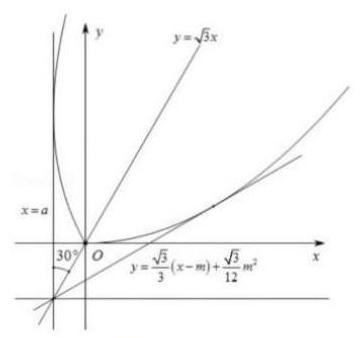
\includegraphics[max width=0.3\textwidth]{images/bo_d5jma53ef24c73bll4ig_28_301_239_360_338_0.jpg}
\end{center}
\hspace*{3em} 

由 \(\left\{  \begin{array}{l} y = \frac{\sqrt{3}}{3}\left( {x - m}\right)  + \frac{\sqrt{3}}{12}{m}^{2} \\  y = \frac{\sqrt{3}}{12}{x}^{2} \end{array}\right.\) 得 \({x}^{2} - {4x} + {4m} - {m}^{2} = 0\) ,

则 \(\Delta  = {16} - {16m} + 4{m}^{2} = 0\) ,解得 \(m = 2\) ,由图像得 \(0 < m \leq  2\) ,

所以实数 \(m\) 的取值范围为 \((0,2\rbrack\) .

【练习】4. (2025 届华二) 已知函数 \(f\left( x\right)\) 不是常数函数,且满足对于任意的 \(a\text{ 、 }b \in  R,f\left( {a + b}\right)  + \; f\left( {a - b}\right)  = {2f}\left( a\right) f\left( b\right)\) ,则 ( )

A. \(f\left( 0\right)  = 0\) B. \(f\left( x\right)\) 一定为周期函数

C. \(f\left( x\right)\) 不可能为奇函数 D. 存在 \({x}_{0} \in  R,f\left( {x}_{0}\right)  =  - 2\)

【答案】 \(C\)

【解析】令 \(a = b = 0\) ,解得 \(f\left( 0\right)  = 0\) 或 \(f\left( 0\right)  = 1\) .

若 \(f\left( 0\right)  = 0\) ,令 \(a = x,b = 0\) ,则 \(f\left( x\right)  + f\left( x\right)  = 0\) ,

所以 \(f\left( x\right)  = 0\) ,与函数不为常数函数矛盾,所以 \(f\left( 0\right)  = 1\) ,故 \(A\) 错误;

令 \(a = 0,b = x\) ,得 \(f\left( x\right)  + f\left( {-x}\right)  = {2f}\left( x\right)\) ,所以 \(f\left( {-x}\right)  = f\left( x\right)\) ,

又因为 \(x \in  R\) ,所以 \(f\left( x\right)\) 必然为偶函数,故 \(C\) 正确;

令 \(a = b = \frac{x}{2}\) ,则 \(f\left( x\right)  = 2{f}^{2}\left( \frac{x}{2}\right)  - 1 \geq   - 1\) ,

所以不存在 \({x}_{0} \in  R\) ,使 \(f\left( {x}_{0}\right)  =  - 2\) 成立，故 \(D\) 错误；

而 \(f\left( x\right)  = \frac{{\mathrm{e}}^{x} + {\mathrm{e}}^{-x}}{2}\) 符合题意且在 \(\left( {0, + \infty }\right)\) 上单调递增,

故其可能不为周期函数，即 \(B\) 错误.

故选 \(C\) .

【练习】5. 设 \(h\left( x\right) \text{ 、 }g\left( x\right)\) 是定义在 \(R\) 上的两个函数,若 \(\forall {x}_{1}\text{ 、 }{x}_{2} \in  R,{x}_{1} \neq  {x}_{2}\) ,有 \(\left| {h\left( {x}_{1}\right)  - h\left( {x}_{2}\right) }\right|  \geq \; \left| {g\left( {x}_{1}\right)  - g\left( {x}_{2}\right) }\right|\) 恒成立，下列四个命题正确的是 ( )

A. 若 \(h\left( x\right)\) 是奇函数，则 \(g\left( x\right)\) 也一定是奇函数

B. 若 \(g\left( x\right)\) 是偶函数，则 \(h\left( x\right)\) 也一定是偶函数

C. 若 \(h\left( x\right)\) 是周期函数，则 \(g\left( x\right)\) 也一定是周期函数

D. 若 \(h\left( x\right)\) 是 \(R\) 上的增函数，则 \(H\left( x\right)  = h\left( x\right)  - g\left( x\right)\) 在 \(R\) 上一定是减函数

【答案】 \(C\)

【解析】对于 \(A\) ,令 \(h\left( x\right)  = x,g\left( x\right)  = 1\) ,对 \(\forall {x}_{1}\text{ 、 }{x}_{2} \in  R,{x}_{1} \neq  {x}_{2}\) ,

得 \(\left| {h\left( {x}_{1}\right)  - h\left( {x}_{2}\right) }\right|  = \left| {{x}_{1} - {x}_{2}}\right|  \geq  \left| {1 - 1}\right|  = \left| {g\left( {x}_{1}\right)  - g\left( {x}_{2}\right) }\right|\) ,而此时 \(g\left( x\right)\) 不是奇函数,故错误;

对于 \(B\) ,令 \(h\left( x\right)  = x,g\left( x\right)  = 1,g\left( x\right)\) 是偶函数,对 \(\forall {x}_{1}\text{ 、 }{x}_{2} \in  R,{x}_{1} \neq  {x}_{2}\) ,

得 \(\left| {h\left( {x}_{1}\right)  - h\left( {x}_{2}\right) }\right|  = \left| {{x}_{1} - {x}_{2}}\right|  \geq  \left| {1 - 1}\right|  = \left| {g\left( {x}_{1}\right)  - g\left( {x}_{2}\right) }\right|\) ,此时 \(h\left( x\right)\) 为奇函数,

故错误;

对于 \(C\) ,设 \(h\left( x\right)\) 的周期为 \(T\) ,

若 \(\forall {x}_{1}\text{ 、 }{x}_{2} \in  R,{x}_{1} \neq  {x}_{2}\) ,有 \(\left| {h\left( {x}_{1}\right)  - h\left( {x}_{2}\right) }\right|  \geq  \left| {g\left( {x}_{1}\right)  - g\left( {x}_{2}\right) }\right|\) 恒成立,

令 \({x}_{1} = x + T,{x}_{2} = x\) ,则 \(\left| {h\left( {x + T}\right)  - h\left( x\right) }\right|  \geq  \left| {g\left( {x + T}\right)  - g\left( x\right) }\right|\) ,

因为 \(h\left( {x + T}\right)  = h\left( x\right)\) ,所以 \(\left| {g\left( {x + T}\right)  - g\left( x\right) }\right|  \leq  0\) ,所以 \(g\left( {x + T}\right)  = g\left( x\right)\) ,

所以函数 \(y = g\left( x\right)\) 也是周期函数，故正确；

对于 \(D\) ,设 \({x}_{1} < {x}_{2},h\left( x\right)\) 是 \(R\) 上的增函数,所以 \(h\left( {x}_{1}\right)  < h\left( {x}_{2}\right)\) ,

又 \(\left| {h\left( {x}_{1}\right)  - h\left( {x}_{2}\right) }\right|  \geq  \left| {g\left( {x}_{1}\right)  - g\left( {x}_{2}\right) }\right|\) ,

即为 \(h\left( {x}_{1}\right)  - h\left( {x}_{2}\right)  \leq  g\left( {x}_{1}\right)  - g\left( {x}_{2}\right)  \leq  h\left( {x}_{2}\right)  - h\left( {x}_{1}\right)\) ,

即为 \(h\left( {x}_{1}\right)  - g\left( {x}_{1}\right)  \leq  h\left( {x}_{2}\right)  - g\left( {x}_{2}\right)\) ,

所以函数 \(y = h\left( x\right)  - g\left( x\right)\) 也都是 \(R\) 上的单调递增函数,故错误.

故选 \(C\) .

【练习】6. (2025 届华二) 已知函数 \(f\left( x\right)\) 的定义域为 \(R\) ,且 \(f\left( {1 + x}\right)  + f\left( {1 - x}\right)  = f\left( x\right) ,f\left( 0\right)  = 2\) ,则 \(f\left( {2024}\right)  + f\left( {2026}\right)  =\) ( )

A. 1 B. 2 C. -1 D. -2

【答案】 \(D\)

【解析】因为函数 \(f\left( x\right)\) 的定义域为 \(R\) ,且 \(f\left( {1 + x}\right)  + f\left( {1 - x}\right)  = f\left( x\right)\)  \circled{1} ,

在 \circled{1} 式中，用 \(- x\) 替换 \(x\) ，得 \(f\left( {1 - x}\right)  + f\left( {1 + x}\right)  = f\left( {-x}\right)\)  \circled{2} ，

由 \circled{1}  \circled{2} 得 \(f\left( {-x}\right)  = f\left( x\right)\) ，所以函数 \(f\left( x\right)\) 为偶函数.

在 \circled{1} 式中，令 \(x = 0\) ，得 \({2f}\left( 1\right)  = f\left( 0\right)  = 2 \Rightarrow  f\left( 1\right)  = 1\) ；

另,令 \(x = 1\) ,得 \(f\left( 2\right)  + f\left( 0\right)  = f\left( 1\right)\) ,所以 \(f\left( 2\right)  = f\left( 1\right)  - f\left( 0\right)  = 1 - 2 =  - 1\) ;

令 \(x = 2\) ,得 \(f\left( 3\right)  + f\left( {-1}\right)  = f\left( 2\right)\) ,所以 \(f\left( 3\right)  = f\left( 2\right)  - f\left( {-1}\right)  =  - 1 - 1 =  - 2\) ;

令 \(x = 3\) ,得 \(f\left( 4\right)  + f\left( {-2}\right)  = f\left( 3\right)\) ,

所以 \(f\left( 4\right)  = f\left( 3\right)  - f\left( {-2}\right)  = f\left( 3\right)  - f\left( 2\right)  =  - 2 + 1 =  - 1\) .

在 \circled{1} 式中，用 \(x + 1\) 替换 \(x\) ，得 \(f\left( {2 + x}\right)  + f\left( {-x}\right)  = f\left( {x + 1}\right)\)

\(\Rightarrow  f\left( {2 + x}\right)  + f\left( x\right)  = f\left( {x + 1}\right)  \Rightarrow  f\left( x\right)  = f\left( {x + 1}\right)  - f\left( {x + 2}\right)\) ,

迭代得 \(f\left( x\right)  = f\left( {x + 1}\right)  - f\left( {x + 2}\right)  = f\left( {x + 2}\right)  - f\left( {x + 3}\right)  - f\left( {x + 2}\right)  =  - f\left( {x + 3}\right)\) ,

\(f\left( {x + 3}\right)  =  - f\left( x\right)\) ,所以 \(f\left( {x + 6}\right)  =  - f\left( {x + 3}\right)  = f\left( x\right)\) ,

故 \(f\left( x\right)\) 是以 6 为周期的周期函数,

所以 \(f\left( {2024}\right)  = f\left( {{337} \times  6 + 2}\right)  = f\left( 2\right)  =  - 1\) ,

\(f\left( {2026}\right)  = f\left( {{337} \times  6 + 4}\right)  = f\left( 4\right)  =  - 1\) ,所以 \(f\left( {2024}\right)  + f\left( {2026}\right)  =  - 2\) .

故选 \(D\) .

【练习】7. 函数 \(f\left( x\right)  = \sqrt{1 - {x}^{2}}, - \frac{1}{2} \leq  x \leq  \frac{1}{2}\) 的图像绕着原点旋转弧度 \(\theta \left( {0 \leq  \theta  \leq  \pi }\right)\) ,若得到的图像仍是函数图像,则 \(\theta\) 可取值的集合为\_\_\_\_\_.

【答案】 \(\left\lbrack  {0,\frac{\pi }{3}}\right\rbrack   \cup  \left\lbrack  {\frac{2\pi }{3},\pi }\right\rbrack\)

【解析】画出函数 \(f\left( x\right)  = \sqrt{1 - {x}^{2}}, - \frac{1}{2} \leq  x \leq  \frac{1}{2}\) 的图象,如图 1 所示: 2025 版上海高考真题及模拟训练合集

\begin{center}
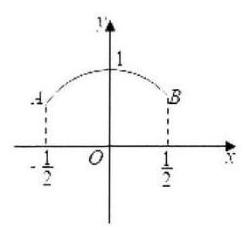
\includegraphics[max width=0.2\textwidth]{images/bo_d5jma53ef24c73bll4ig_30_298_245_243_230_0.jpg}
\end{center}
\hspace*{3em} 

图 1

\begin{center}
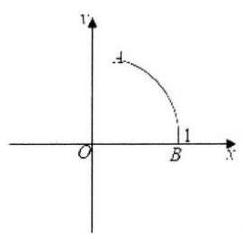
\includegraphics[max width=0.2\textwidth]{images/bo_d5jma53ef24c73bll4ig_30_593_238_243_239_0.jpg}
\end{center}
\hspace*{3em} 

图 2

\begin{center}
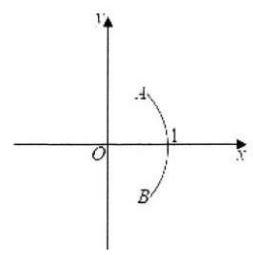
\includegraphics[max width=0.2\textwidth]{images/bo_d5jma53ef24c73bll4ig_30_288_489_253_255_0.jpg}
\end{center}
\hspace*{3em} 

图 3

\begin{center}
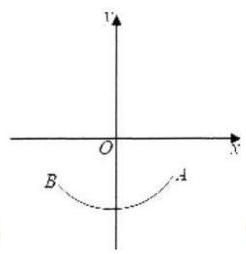
\includegraphics[max width=0.2\textwidth]{images/bo_d5jma53ef24c73bll4ig_30_591_489_246_254_0.jpg}
\end{center}
\hspace*{3em} 

图 4

圆弧所在圆的方程为 \({x}^{2} + {y}^{2} = 1,A\left( {-\frac{1}{2},\frac{\sqrt{3}}{2}}\right) ,B\left( {\frac{1}{2},\frac{\sqrt{3}}{2}}\right)\) ,

在图象绕原点旋转的过程中,当点 \(B\) 从图 1 的位置旋转到 \(\left( {1,0}\right)\) 点时,

由函数的定义得这个旋转过程所得的图形均为函数的图象,如图 2 所示:

此时绕着原点旋转弧度为 \(0 \leq  \theta  \leq  \frac{\pi }{3}\) .

若函数图象在图 2 位置绕着原点继续旋转,

当点 \(B\) 在 \(x\) 轴下方,点 \(A\) 在 \(x\) 轴上方时,

由函数的定义得,所得图形不是函数的图象,如图 3 所示:

此时转过的角度为 \(\frac{\pi }{3} < \theta  < \frac{2\pi }{3}\) ,不满足题意; 67

若函数图象在图 3 位置绕着原点继续旋转，当整个图象都在 \(x\) 轴下方时，

由函数的定义得,所得图形是函数的图象,如图 4 所示:

此时转过的角度为 \(\frac{2\pi }{3} \leq  \theta  \leq  \pi\) ;

综上, \(\theta\) 的可取值集合为 \(\left\lbrack  {0,\frac{\pi }{3}}\right\rbrack   \cup  \left\lbrack  {\frac{2\pi }{3},\pi }\right\rbrack\) .

【练习】8. (2025 届交附) 设定义域为 \(R\) 的函数 \(y = f\left( x\right)\) 满足 \(f\left( {x - 2}\right)  = {2f}\left( x\right)\) ,当 \(x \in  \lbrack  - 2,0)\) 时, \(f\left( x\right) \; =  - {2x}\left( {x + 2}\right)\) . 若对任意 \(x \in  \lbrack m, + \infty )\) ，都有 \(f\left( x\right)  \leq  \frac{3}{4}\) ，则实数 \(m\) 的取值范围是\_\_\_\_\_

A. \(\left\lbrack  {\frac{2}{3}, + \infty }\right)\) B. \(\left\lbrack  {\frac{3}{4}, + \infty }\right)\) C. \(\left\lbrack  {\frac{1}{2}, + \infty }\right)\) D. \(\left\lbrack  {\frac{3}{2}, + \infty }\right)\)

【答案】 \(D\)

【解析】当 \(x \in  \lbrack  - 2,0)\) 时,函数 \(f\left( x\right)\) 在 \(\left( {-2, - 1}\right)\) 上严格增,在 \(\left( {-1,0}\right)\) 上严格减,

所以 \(f{\left( x\right) }_{\max } = f\left( {-1}\right)  = 2\) ,

由 \(f\left( {x - 2}\right)  = {2f}\left( x\right)\) 得 \(\frac{1}{2}f\left( {x - 2}\right)  = f\left( x\right)\) ,得当图象向右平移 2 个单位时,

最大值变为原来的 \(\frac{1}{2}\) 倍,最大值不断变小,

由 \(f\left( {x - 2}\right)  = {2f}\left( x\right)\) 得 \(f\left( x\right)  = {2f}\left( {x + 2}\right)\) ，得当图象向左平移 2 个单位时，

最大值变为原来的 2 倍，最大值不断变大，

2025 版上海高考真题及模拟训练合集

\begin{center}
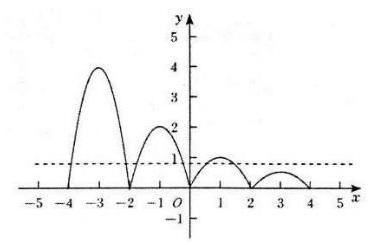
\includegraphics[max width=0.3\textwidth]{images/bo_d5jma53ef24c73bll4ig_31_295_232_368_245_0.jpg}
\end{center}
\hspace*{3em} 

当 \(x \in  \lbrack 0,2)\) 时, \(f{\left( x\right) }_{\max } = f\left( 1\right)  = 1\) ,

当 \(x \in  \lbrack 2,4)\) 时， \(f{\left( x\right) }_{\max } = f\left( 3\right)  = \frac{1}{2}\) ，

设 \(x \in  \lbrack 0,2)\) ,则 \(x - 2 \in  \lbrack  - 2,0),f\left( {x - 2}\right)  =  - {2x}\left( {x - 2}\right)  = {2f}\left( x\right)\) ,

即 \(f\left( x\right)  =  - x\left( {x - 2}\right)\) ,由 \(- x\left( {x - 2}\right)  = \frac{3}{4}\) ,解得 \(x = \frac{1}{2}\) 或 \(x = \frac{3}{2}\) ,

由题意得当 \(m \geq  \frac{3}{2}\) 时, \(f\left( x\right)  \leq  \frac{3}{4}\) 恒成立,故选 \(D\)

【练习】9. (2025 届华二) 已知函数 \(y = f\left( x\right)\) 具有以下的性质:对于任意实数 \(a\) 和 \(b\) ,都有 \(f\left( {a + b}\right)  + \; f\left( {a - b}\right)  = {2f}\left( a\right)  \cdot  f\left( b\right)\) ,则以下选项中,不可能是 \(f\left( 1\right)\) 值的是 ( )

A. -2 B. -1 C. 0 D. 1

【答案】 \(A\)

【解析】在 \(f\left( {a + b}\right)  + f\left( {a - b}\right)  = {2f}\left( a\right)  \cdot  f\left( b\right)\) 中,

令 \(a = b = 0\) ,得 \({2f}\left( 0\right)  = 2{f}^{2}\left( 0\right)\) ,所以 \(f\left( 0\right)  = 0\) 或 1,

令 \(a = b = \frac{x}{2}\) ,得 \(f\left( x\right)  + f\left( 0\right)  = 2{f}^{2}\left( \frac{x}{2}\right)  \geq  0\) ,则 \(f\left( x\right)  \geq   - 1\) ,故选 \(A\) .

【练习】10. (2025 届华二) 对于两个定义在 \(R\) 上的函数 \(y = f\left( x\right)\) 与 \(y = g\left( x\right)\) ,构造新函数 \(y = h\left( x\right)\) 如下: 对任意 \({x}_{0} \in  R,h\left( {x}_{0}\right)  = f\left( {x}_{0}\right)  + g\left( {x}_{0}\right)\) . 现已知 \(y = h\left( x\right)\) 是严格增函数,对于以下两个命题:

 \circled{1}  \(y = f\left( x\right)\) 与 \(y = g\left( x\right)\) 中至少有一个是严格增函数;

 \circled{2}  \(y = f\left( x\right)\) 与 \(y = g\left( x\right)\) 中至少有一个函数无最大值. 其中 ( )

A.  \circled{1} 和 \circled{2} 都是真命题 B. 只有 \circled{1} 是真命题

C. 只有 \circled{2} 是真命题 D. 没有真命题

【答案】 \(D\)

【解析】令 \(f\left( x\right)  = \left\{  {\begin{array}{l} \sin x,x \leq  0 \\   - \sin x,x > 0 \end{array},g\left( x\right)  = \left\{  \begin{array}{l}  - \sin x - {\mathrm{e}}^{-x},x \leq  0 \\  \sin x - {\mathrm{e}}^{-x},x > 0 \end{array}\right. }\right.\) ,则没有真命题,故选 \(D\) .

\section*{板块三:压轴客观题}

\section*{1. 真题回顾}

【例题】1. (2024 上海秋考) 已知定义在 \(R\) 上的函数 \(y = f\left( x\right) ,M = \left\{  {x}_{0}\right|\) 对于任意 \(x \in  \left( {-\infty ,{x}_{0}}\right) ,f\left( x\right)  < \; \left. {f\left( {x}_{0}\right) }\right\}\) . 对于所有 \(M = \left\lbrack  {-1,1}\right\rbrack\) 的函数 \(y = f\left( x\right)\) ,以下说法正确的是 ( )

A. 存在 \(y = f\left( x\right)\) 是偶函数 B. 存在 \(y = f\left( x\right)\) 在 \(x = 2\) 处取到最大值

C. 存在 \(y = f\left( x\right)\) 是严格增函数 D. 存在 \(y = f\left( x\right)\) 在 \(x =  - 1\) 处取到极小值

【答案】 \(B\)

【解析】对于 \(A\) ,若存在 \(y = f\left( x\right)\) 是偶函数,取 \({x}_{0} = 1 \in  \left\lbrack  {-1,1}\right\rbrack\) ,

则对于任意 \(x \in  \left( {-\infty ,1}\right) ,f\left( x\right)  < f\left( 1\right)\) ,而 \(f\left( {-1}\right)  = f\left( 1\right)\) ,矛盾,故 \(A\) 错误;

对于 \(B\) ,取 \({x}_{0} \in  \left\lbrack  {-1,1}\right\rbrack  ,y = f\left( x\right)  = \left\{  \begin{array}{ll}  - 2, & x <  - 1 \\  x, &  - 1 \leq  x < 1, \\  1, & x \geq  1 \end{array}\right.\) 满足题意，故 \(B\) 错误；

对于 \(C\) ,若存在 \(y = f\left( x\right)\) 是严格增函数，则 \(M = R\) 与 \(M = \left\lbrack  {-1,1}\right\rbrack\) 矛盾，

故 \(C\) 错误;

对于 \(D\) ,存在 \(y = f\left( x\right)\) 在 \(x =  - 1\) 处取到极小值,则在 -1 附近,存在 \(t\) ,

\(f\left( t\right)  \geq  f\left( {-1}\right)\) ,矛盾,故 \(D\) 错误;

故选 \(B\) .

【例题】2. (2024 上海春考) 现定义如下: 当 \(x \in  \left( {n,n + 1}\right) ,n \in  N\) 时, \(f\left( {x + 1}\right)  = {f}^{\prime }\left( x\right)\) ,则称 \(f\left( x\right)\) 为延展函数. 满足当 \(x \in  \left( {0,1}\right)\) 时, \(g\left( x\right)  = {\mathrm{e}}^{x}\) 与 \(h\left( x\right)  = {x}^{10}\) 均为延展函数,现有如下两个命题:

 \circled{1}  存在 \(y = {kx} + b\left( {k,b \in  R;k,b \neq  0}\right)\) 与 \(y = g\left( x\right)\) 有无穷个交点;

 \circled{2} 存在 \(y = {kx} + b\left( {k,b \in  R;k,b \neq  0}\right)\) 与 \(y = h\left( x\right)\) 有无穷个交点;

则下列说法正确的是 ( )

A.  \circled{1} 正确， \circled{2} 正确 B.  \circled{1} 不正确， \circled{2} 不正确

C.  \circled{1} 正确， \circled{2} 不正确 D.  \circled{1} 不正确， \circled{2} 正确

【答案】 \(D\)

【解析】由 \(f\left( {x + 1}\right)  = {f}^{\prime }\left( x\right)\) 得 \(f\left( {x + 1}\right)  = {f}^{\prime }\left( x\right)  \Rightarrow  f\left( x\right)  = {f}^{\prime }\left( {x - 1}\right)\) ,

当 \(x \in  \left( {n + k,n + 1 + k}\right)\) 时, \(x \in  \left( {n + k,n + 1 + k}\right) ,x - k \in  \left( {n,n + 1}\right)\) ,

所以 \(f\left( x\right)  = {f}^{\prime }\left( {x - 1}\right)  = {f}^{\prime \prime }\left( {x - 2}\right)  = \cdots  = {f}^{\left( k\right) }\left( {x - k}\right) ,g\left( x\right)  = {\mathrm{e}}^{x},{g}^{\left( k\right) }\left( x\right)  = {\mathrm{e}}^{x},h\left( x\right)  = {x}^{10},{h}^{\prime }\left( x\right)  = \; {10}{x}^{9},{h}^{\prime \prime }\left( x\right)  = {P}_{10}^{2} \cdot  {x}^{8},\cdots ,{h}^{\left( k\right) }\left( x\right)  = {P}_{10}^{k} \cdot  {x}^{{10} - k},\)

\begin{center}
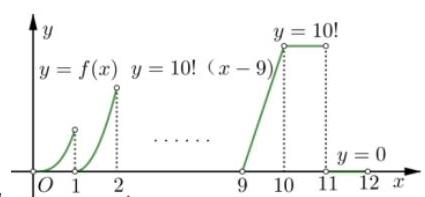
\includegraphics[max width=0.3\textwidth]{images/bo_d5jma53ef24c73bll4ig_32_1038_1624_425_197_0.jpg}
\end{center}
\hspace*{3em} 

当 \(x \in  \left( {k,1 + k}\right)\) 时, \(x \in  \left( {k,1 + k}\right) ,x - k \in  \left( {0,1}\right)\) ,

\({g}_{k}\left( x\right)  = {\mathrm{e}}^{x - k},{h}_{k}\left( x\right)  = {P}_{10}^{k} \cdot  {\left( x - k\right) }^{{10} - k},\)

其中,当 \(x \in  \left( {9,{10}}\right)\) 时, \({h}_{9}\left( x\right)  = {P}_{10}^{9} \cdot  \left( {x - 9}\right)\) 恰为一次函数, 作出函数 \(g\left( x\right)\) 图像,当 \(k \neq  0\) 时,不可能有无穷多个交点; 作出函数 \(h\left( x\right)\) 图像,当 \(k = {P}_{10}^{9}\) 时,存在 \(b =  - 9{P}_{10}^{9}\) ,使得直线 \(y \; = {kx} + b\) 可以与 \(h\left( x\right)\) 在区间 \(\left( {9,{10}}\right)\) 的函数部分重合,从而产生无穷多个交点,

\begin{center}
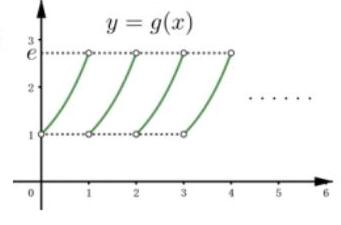
\includegraphics[max width=0.2\textwidth]{images/bo_d5jma53ef24c73bll4ig_32_1125_1820_341_225_0.jpg}
\end{center}
\hspace*{3em} 

故选 \(D\) .

【例题】3. (2022 上海秋考) 函数 \(f\left( x\right)\) 满足 \(f\left( x\right)  = f\left( \frac{1}{1 + x}\right)\) 对任意 \(x \in  \lbrack 0\) , \(+ \infty )\) 都成立,其值域是 \({A}_{f}\) ,已知对任何满足上述条件的 \(f\left( x\right)\) 都有 \(\{ y \mid  y = f\left( x\right) ,0 \leq  x \leq  a\}  = \; {A}_{f}\) ，则 \(a\) 的取值范围为\_\_\_\_\_.

【答案】 \(\left\lbrack  {\frac{\sqrt{5} - 1}{2}, + \infty }\right)\)

【解析】法一: 令 \(x = \frac{1}{x + 1}\) ,解得 \(x = \frac{\sqrt{5} - 1}{2}\) (负值舍去),

当 \({x}_{1} \in  \left\lbrack  {0,\frac{\sqrt{5} - 1}{2}}\right\rbrack\) 时, \({x}_{2} = \frac{1}{{x}_{1} + 1} \in  \left\lbrack  {\frac{\sqrt{5} - 1}{2},1}\right\rbrack\) ,

当 \({x}_{1} \in  \left( {\frac{\sqrt{5} - 1}{2}, + \infty }\right)\) 时, \({x}_{2} = \frac{1}{{x}_{1} + 1} \in  \left( {0,\frac{\sqrt{5} - 1}{2}}\right)\) ,

且当 \({x}_{1} \in  \left( {\frac{\sqrt{5} - 1}{2}, + \infty }\right)\) 时,总存在 \({x}_{2} = \frac{1}{{x}_{1} + 1} \in  \left( {0,\frac{\sqrt{5} - 1}{2}}\right)\) ,使得 \(f\left( {x}_{1}\right)  = f\left( {x}_{2}\right)\) ,

故 \(f\left( \left\lbrack  {0,\frac{\sqrt{5} - 1}{2}}\right\rbrack  \right)  = {A}_{f}\) ,若 \(a < \frac{\sqrt{5} - 1}{2}\) ,易得 \(f\left( \frac{\sqrt{5} - 1}{2}\right)  \notin  f\left( \left\lbrack  {0,a}\right\rbrack  \right)\) ,

所以 \(a \geq  \frac{\sqrt{5} - 1}{2}\) ,即实数 \(a\) 的取值范围为 \(\left\lbrack  {\frac{\sqrt{5} - 1}{2}, + \infty }\right)\) .

法二: 原命题等价于任意 \(a > 0,f\left( {x + a}\right)  = f\left( \frac{1}{1 + x + a}\right)\) ,

所以 \(a > 0,f\left( {x + a}\right)  = f\left( \frac{1}{1 + x + a}\right)  \Rightarrow  \frac{1}{1 + x + a} \leq  a \Rightarrow  x \geq  \frac{1}{a} - \left( {1 + a}\right)\) 恒成立,即 \(\frac{1}{a} - (1 + \; a) \leq  0\) 恒成立,

所以 \(a \geq  \frac{\sqrt{5} - 1}{2}\) ,即实数 \(a\) 的取值范围为 \(\left\lbrack  {\frac{\sqrt{5} - 1}{2}, + \infty }\right)\) .

【例题】4. (2019 上海秋考) 已知 \(f\left( x\right)  = \left| {\frac{2}{x - 1} - a}\right| \left( {x > 1,a > 0}\right) ,f\left( x\right)\) 与 \(x\) 轴交点为 \(A\) ,若对于 \(f\left( x\right)\) 图象上任意一点 \(P\) ，在其图象上总存在另一点 \(Q\left( {P\text{ 、 }Q\text{ 异于 }A}\right)\) ，满足 \({AP}\bot {AQ}\) ，且 \(\left| {AP}\right|  = \left| {AQ}\right|\) ， 则 \(a =\) \_\_\_\_\_.

【答案】 \(\sqrt{2}\)

【解析】法一: (设而不求),设 \(P\left( {x,y}\right) \left( {x < \frac{2}{a} + 1}\right)\) ,

\begin{center}
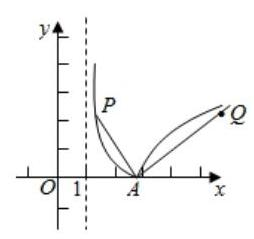
\includegraphics[max width=0.2\textwidth]{images/bo_d5jma53ef24c73bll4ig_33_1199_1326_254_239_0.jpg}
\end{center}
\hspace*{3em} 

易得点 \(A\left( {\frac{2}{a} + 1,0}\right)\) 且 \(y = \frac{2}{x - 1} - a\)  \circled{1} .

因为 \({AP} \bot  {AQ}\) 且 \(\left| {AP}\right|  = \left| {AQ}\right|\) ,所以 \(Q\left( {\frac{2}{a} + 1 + y,\frac{2}{a} + 1 - x}\right)\) .

(因为 \(\overrightarrow{AP} = \left( {x - \frac{2}{a} - 1,y}\right)\) ,顺时计旋转 \(\frac{\pi }{2}\) ,

得 \(\overrightarrow{AQ} = \left( {y, - x + \frac{2}{a} + 1}\right)  = \left( {{x}_{Q} - \frac{2}{a} - 1,{y}_{Q}}\right)\) ,所以 \(\left\{  \begin{array}{l} {x}_{Q} = \frac{2}{a} + 1 + y \\  {y}_{Q} = \frac{2}{a} + 1 - x \end{array}\right)\)

把点 \(Q\) 坐标代入 \(y = a - \frac{2}{x - 1}\) 得 \(\frac{2}{a} + 1 - x = a - \frac{2}{\frac{2}{a} + y}\)  \circled{2} .

消去 \(y\) (或 \(x\) ). \(y = \frac{2}{x - 1} - a\)  \circled{1}  \(y = \frac{2}{x - 1} - a\) (1) \(\Rightarrow  \frac{2}{a} + 1 - x = a - \frac{2}{\frac{2}{a} + y}\)  \circled{2} ,

由 \circled{1} 得 \(x - 1 = \frac{2}{y + a}\) ，代入 \circled{2} 得 \(\frac{2}{a} - \frac{2}{y + a} = a - \frac{2}{\frac{2}{a} + y}\) ，

所以 \(\left( {\frac{2}{a} - a}\right) {y}^{2} + \left( {\frac{2}{a} - a}\right) \left( {a + \frac{2}{a}}\right) y + 2\left( {\frac{2}{a} - a}\right)  - \frac{4}{a} + {2a} = 0\) 恒成立,

所以 \(\frac{2}{a} - a = \left( {\frac{2}{a} - a}\right) \left( {a + \frac{2}{a}}\right)  = 2\left( {\frac{2}{a} - a}\right)  - \frac{4}{a} + {2a} = 0\) ,

又因为 \(a > 0\) ,故 \(a = \sqrt{2}\) .

法二: 在法一的 \(y = \frac{2}{x - 1} - a\)  \circled{1}  \(y = \frac{2}{x - 1} - a\) (1) \(\Rightarrow  \frac{2}{a} + 1 - x = a - \frac{2}{\frac{2}{a} + y}\)  \circled{2} ,

消去 \({xy}\) . 由 \circled{1} 得 \({xy} = 2 + a + y - {ax}\)  \circled{3} ，

由 \circled{2} 得 \({xy} = \left( {\frac{2}{a} + 1 - a}\right) y - \frac{2}{a}x + \left( {\frac{4}{{a}^{2}} + \frac{2}{a}}\right)\)  \circled{4} .

把 \circled{3} 代入 \circled{4} ，所以 \(\left( {2 + a - \frac{4}{{a}^{2}} - \frac{2}{a}}\right)  + \left( {\frac{2}{a} - a}\right) x + \left( {a - \frac{2}{a}}\right) y = 0\) 恒成立，

所以 \(2 + a - \frac{4}{{a}^{2}} - \frac{2}{a} = \frac{2}{a} - a = a - \frac{2}{a} = 0\) ,又因为 \(a > 0\) ,故 \(a = \sqrt{2}\) .

法三: 联立方程组,设直线 \({AQ} : x = {my} + 1 + \frac{2}{a},{AP} : x =  - \frac{1}{m}y + 1 + \frac{2}{a}\left( {m > 0}\right)\) .

易得点 \(A\left( {\frac{2}{a} + 1,0}\right)\) . 联立方程组 \(\left\{  \begin{array}{l} x = {my} + 1 + \frac{2}{a} \\  y = a - \frac{2}{x - 1} \end{array}\right.\) ,得 \({y}_{Q} = a - \frac{2}{am}\) ,

同理 \({y}_{P} = \frac{2m}{a} - a\) . 所以 \(\left\{  \begin{array}{l} \left| {AQ}\right|  = \sqrt{{m}^{2} + 1} \cdot  \left| {{y}_{Q} - 0}\right|  = \sqrt{{m}^{2} + 1} \cdot  \left( {a - \frac{2}{am}}\right) \\  \left| {AP}\right|  = \sqrt{\frac{1}{{m}^{2}} + 1} \cdot  \left| {{y}_{P} - 0}\right|  = \frac{\sqrt{{m}^{2} + 1}}{m} \cdot  \left( {\frac{2m}{a} - a}\right)  \end{array}\right.\) ,

因为 \(\left| {AP}\right|  = \left| {AQ}\right|\) 对许多 \(m \in  {R}^{ + }\) 恒成立,整理得 \(\left( {a - \frac{2}{a}}\right) m = \frac{2}{a} - a\) ,

所以 \(a - \frac{2}{a} = \frac{2}{a} - a = 0\) ,又因为 \(a > 0\) ,故 \(a = \sqrt{2}\) .

法四:极限思想 \(\left( {x\text{ 趋向于两边 }}\right)\) . 易得点 \(A\left( {1 + \frac{2}{a},0}\right)\) .

过点 \(P\text{ 、 }Q\) 分别作 \({PM} \bot  x\) 轴、 \({QN} \bot  x\) 轴,垂足为 \(M\text{ 、 }N\) .

因为 \({AP} \bot  {AQ}\) 且 \(\left| {AP}\right|  = \left| {AQ}\right|\) ,所以 \(\bigtriangleup {APM} \cong  \bigtriangleup {OAN}\) ,所以 \(\left| {AM}\right|  = \left| {QN}\right|\) .

当点 \(P\) 无限接近 \(f\left( x\right)\) 的渐近线时,点 \(Q\) 也无限接近 \(f\left( x\right)\) 的渐近线,

即 \(\left| {AM}\right|\) 无限趋近于 \(1 + \frac{2}{a} - 1 = \frac{2}{a},\left| {QN}\right|\) 无限趋近于 \(a\) ,

所以 \(\frac{2}{a} = a\) ,又因为 \(a > 0\) ,故 \(a = \sqrt{2}\) .

法五:极限思想 \(\left( {x\text{ 趋向于点 }A}\right)\) . 易得点 \(A\left( {1 + \frac{2}{a},0}\right)\) .

当点 \(P\) 无限接近点 \(A\) 割,割线 \({AP}\) 退化为 \(f\left( x\right)\) 在点 \(A\) 处的 (左) 切线,

设切线斜率为 \(k\) . 因为 \(\left| {AP}\right|  = \left| {AQ}\right|\) ,所以此割点 \(Q\) 也无限接近点 \(A\) ,

此时 \(y = f\left( x\right)\) 在点 \(A\) 处的 (右) 切线斜率应与 \(y =  - f\left( x\right)\)

在点 \(A\) 处的 (右) 切线斜率相反,即为 \(- k\) .

因为 \({AP} \bot  {AQ}\) ,所以 \(k \cdot  \left( {-k}\right)  =  - 1\) ,解得 \(k =  - 1\) .

联立方程组 \(\left\{  \begin{array}{l} y =  - x + 1 + \frac{2}{a} \\  y = \frac{2}{x - 1} - a \end{array}\right.\) ,则 \({x}^{2} - \left( {a + \frac{2}{a} + 2}\right) x + a + \frac{2}{a} + 3 = 0\) ,

由 \(\Delta  = 0\) 且 \(a > 0\) 得 \(a = \sqrt{2}\) .

法六:在函数 \(y = f\left( x\right)\) 上找一个点 \(A\) ，使得被点 \(A\) 分开的两段曲线是 “全等”的.

因为 \(y = \frac{2}{x}\left( {x > 0}\right)\) ，显然顶点 \({A}^{\prime }\left( {\sqrt{2},\sqrt{2}}\right)\) 满足题意，

又 \(y = \frac{2}{x}\left( {x > 0}\right)\) 的图像先向方平移一个单位,

再向下平移 \(a\) 个单位后可以得到 \(f\left( x\right)  = \frac{2}{x - 1} - a\) . 所以 \(a = \sqrt{2}\) .

【例题】5. (2019 上海秋考) 已知 \(\tan \alpha  \cdot  \tan \beta  = \tan \left( {\alpha  + \beta }\right)\) . 有下列两个结论:

 \circled{1} 存在 \(\alpha\) 在第一象限， \(\beta\) 在第三象限； \circled{2} 存在 \(\alpha\) 在第二象限， \(\beta\) 在第四象限； 则 ( )

A.  \circled{1}  \circled{2} 均正确 B.  \circled{1}  \circled{2} 均错误 C.  \circled{1} 对 \circled{2} 错 D.  \circled{1} 错 \circled{2} 对

【答案】 \(D\)

【解析】法一: 令 \(a = \tan \alpha ,b = \tan \beta\) ,则 \({ab} = \frac{a + b}{1 - {ab}} \Rightarrow  \frac{1}{a} + \frac{1}{b} = 1 - {ab}\) .

当 \(a > 1,b > 1\) 时，显然矛盾；

当 \(0 < a < 1,0 < b < 1\) 时, \(\frac{1}{a} + \frac{1}{b} \in  \left( {2, + \infty }\right) ,1 - {ab} \in  \left( {0,1}\right)\) ,也不成立;

由此, 故 \circled{1} 错误;

当 \(a < 0,b < 0\) 时,若 \(a =  - 1\) 时, \(\frac{1}{b} - b = 2,b < 0 \Rightarrow  b =  - 1 - \sqrt{2}\) ,故 \circled{2} 正确.

故选 \(D\) .

法二: 由题意,只讨论 \({ab} > 0,a + b \geq  2\sqrt{ab} \Rightarrow  \sqrt{ab}\left( {1 - {ab}}\right)  \geq  2\) .

当 \(a > 1,b > 1\) 时,显然矛盾;

当 \(0 < a < 1,0 < b < 1\) 时， \(\sqrt{ab}\left( {1 - {ab}}\right)  \in  \left( {0,1}\right)\) ，故 \(\sqrt{ab}\left( {1 - {ab}}\right)  \geq  2\) 也不成立； 由此, 故 \circled{1} 错误;

当 \(a < 0,b < 0\) 时,若 \(a =  - 1\) 时, \(\frac{1}{b} - b = 2,b < 0 \Rightarrow  b =  - 1 - \sqrt{2}\) ,故 \circled{2} 正确.

故选 \(D\) .

法三: \({ab} = \frac{a + b}{1 - {ab}} \Rightarrow  {a}^{2}{b}^{2} + \left( {1 - b}\right) a + b = 0\) (当成关于 \(a\) 的一元二次方程),

对于 \circled{1} ，转化为方程要有大于零的根，

构造二次函数 \(f\left( x\right)  = {b}^{2}{x}^{2} + \left( {1 - b}\right) x + b\) 与 \(x\) 轴正半轴要有交点,

由题意得 \(b > 0\) ,为满足与 \(x\) 轴正半轴要有交点,函数对称轴一定在 \(y\) 轴右侧,

得 \(1 - b < 0\) ,而 \(\Delta  = {\left( 1 - b\right) }^{2} - 4{b}^{3} < 0\left( {{y}_{1} = {\left( 1 - b\right) }^{2},{y}_{2} = 4{b}^{3}}\right.\) , \(\left. {b > 1\text{ 时, }{y}_{2} > {y}_{1}}\right)\) , 故方程此时无大于零的根，故 \circled{1} 错误；

对于 \circled{2} ，转化为方程要有小于零的根，

构造二次函数 \(f\left( x\right)  = {b}^{2}{x}^{2} + \left( {1 - b}\right) x + b\) 与 \(x\) 轴负半轴要有交点,

由题意得 \(b < 0\) ，因为二次函数开口向上，一定与 \(x\) 轴负半轴要有交点，故 \circled{2} 正确. 故选 \(D\) .

法四: \(\alpha \text{ 、 }\beta\) 地位均等,可令 \(\alpha  = \beta\) ,则 \({\tan }^{2}\alpha  = \tan {2\alpha } = \frac{2\tan \alpha }{1 - {\tan }^{2}\alpha }\)

\({\tan }^{2}\alpha  = \tan {2\alpha } = \frac{2\tan \alpha }{1 - {\tan }^{2}\alpha } \Rightarrow  {\tan }^{3}\alpha  =\) ,转化为 \({x}^{3} = x - 2\) ,在 \(\left( {0,1}\right) ,\left( {1, + \infty }\right)\) 无解;

在 \(\left( {-1,0}\right)\) 无解 \(\left( {-\infty , - 1}\right)\) 有一解,所以 \circled{1} 错误, \circled{2} 正确. 故选 \(D\) .

法五: 令 \(\tan \alpha  = x,\tan \beta  = y\) ,则 \({xy} = \frac{x + y}{1 - {xy}} \Rightarrow  1 = {xy} + \frac{x + y}{xy} = {xy} + \frac{1}{x} + \frac{1}{y}\) ,

若 \(x > 0,y > 0\) ,则 \(1 = {xy} + \frac{1}{x} + \frac{1}{y} \geq  3\sqrt[3]{{xy} \cdot  \frac{1}{x} \cdot  \frac{1}{y}} = 3\) ,矛盾,

当 \(x < 0,y < 0\) 时能够成立. 故选 \(D\) .

法六:特殊值法结合计算器的牛顿法解方程,令 \(\tan \alpha  = 3\text{ 、 }\frac{1}{3}\) 和 \(\tan \alpha  =  - 3, - \frac{1}{3}\) ,

求 \(\tan \beta\) 看是否存在 (大部分学生应该是这么做此题的),

故选 \(D\) .

【例题】6. (2019 上海春考) 已知集合 \(A = \left\lbrack  {t,t + 1}\right\rbrack   \cup  \left\lbrack  {t + 4,t + 9}\right\rbrack  ,0 \notin  A\) ,存在正数 \(\lambda\) ,使得对任意 \(a \in \; A\) ,都有 \(\frac{\lambda }{a} \in  A\) ,则 \(t\) 的值是\_\_\_\_\_.

【答案】1 或 -3

【解析】当 \(t > 0\) 时,当 \(a \in  \left\lbrack  {t,t + 1}\right\rbrack\) 时, \(\frac{\lambda }{a} \in  \left\lbrack  {t + 4,t + 9}\right\rbrack\) ,

当 \(a \in  \left\lbrack  {t + 4,t + 9}\right\rbrack\) 时, \(\frac{\lambda }{a} \in  \left\lbrack  {t,t + 1}\right\rbrack\) ,

即当 \(a = t\) 时, \(\frac{\lambda }{a} \leq  t + 9\) ; 当 \(a = t + 9\) 时, \(\frac{\lambda }{a} \geq  t\) ,即 \(\lambda  = t\left( {t + 9}\right)\) ;

当 \(a = t + 1\) 时， \(\frac{\lambda }{a} \geq  t + 4\) ，当 \(a = t + 4\) 时， \(\frac{\lambda }{a} \leq  t + 1\) ，即， \(\lambda  = \left( {t + 1}\right) \left( {t + 4}\right)\) ，

所以 \(t\left( {t + 9}\right)  = \left( {t + 1}\right) \left( {t + 4}\right)\) ,解得 \(t = 1\) .

当 \(t + 1 < 0 < t + 4\) 时,当 \(a \in  \left\lbrack  {t,t + 1}\right\rbrack\) 时, \(\frac{\lambda }{a} \in  \left\lbrack  {t,t + 1}\right\rbrack\) .

当 \(a \in  \left\lbrack  {t + 4,t + 9}\right\rbrack\) 时,则 \(\frac{\lambda }{a} \in  \left\lbrack  {t + 4,t + 9}\right\rbrack\) ,

即当 \(a = t\) 时, \(\frac{\lambda }{a} \leq  t + 1\) ,当 \(a = t + 1\) 时, \(\frac{\lambda }{a} \geq  t\) ,即 \(\lambda  = t\left( {t + 1}\right)\) ,

即当 \(a = t + 4\) 时, \(\frac{\lambda }{a} \leq  t + 9\) ,当 \(a = t + 9\) 时, \(\frac{\lambda }{a} \geq  t + 4\) ,即 \(\lambda  = \left( {t + 4}\right) \left( {t + 9}\right)\) ,

所以 \(t\left( {t + 1}\right)  = \left( {t + 4}\right) \left( {t + 9}\right)\) ,解得 \(t =  - 3\) .

当 \(t + 9 < 0\) 时,同理可得无解.

综上, \(t\) 的值为 1 或 -3 . 2025 版上海高考真题及模拟训练合集

\section*{2. 模拟练习}

【练习】1. (2025 届华二) \(f\left( x\right)\) 在 \(R\) 上非严格递增,满足 \(f\left( {x + 1}\right)  = f\left( x\right)  + 1,g\left( x\right)  = \left\{  \begin{array}{l} f\left( x\right) ,\left| x\right|  < 8 \\  f\left( {x - a}\right) ,\left| x\right|  \geq  8 \end{array}\right.\) , 若存在符合上述要求的函数 \(f\left( x\right)\) 及实数 \({x}_{0}\) ,满足 \(g\left( {{x}_{0} + 4}\right)  = g\left( {x}_{0}\right)  + 1\) ,则 \(a\) 的取值范围是\_\_\_\_\_.

【答案】 \(\left( {-4, - 2}\right)  \cup  \left( {2,4}\right)\)

【解析】 \(f\left( {x + 1}\right)  = f\left( x\right)  + 1\) ,即 \(f\left( {x + 1}\right)  - f\left( x\right)  = 1\) ,

对 \(\forall n \in  {N}^{ * }\) ,则 \(f\left( {x + n}\right)  = \left\lbrack  {f\left( {x + n}\right)  - f\left( {x + n - 1}\right) }\right\rbrack\)

\(+ \left\lbrack  {f\left( {x + n - 1}\right)  - f\left( {x + n - 2}\right) }\right\rbrack   + \cdots  + \left\lbrack  {f\left( {x + 1}\right)  - f\left( x\right) }\right\rbrack   + f\left( x\right)\)

\(= 1 + 1 + \cdots  + 1 + f\left( x\right)  = n + f\left( x\right) ,\)

故对 \(\forall n \in  {N}^{ * }\) ,则 \(f\left( {x + n}\right)  = f\left( x\right)  + n\) ,

因为 \(g\left( {{x}_{0} + 4}\right)  = g\left( {x}_{0}\right)  + 1\) ,

当 \({x}_{0} \leq   - {12}\) 时，则 \({x}_{0} + 4 \leq   - 8\) ，

得 \(f\left( {{x}_{0} + 4 - a}\right)  = f\left( {{x}_{0} - a}\right)  + 4 = f\left( {{x}_{0} - a}\right)  + 1\) ,不成立;

当 \(- {12} < {x}_{0} \leq   - 8\) 时,则 \(- 8 < {x}_{0} + 4 \leq   - 4\) ,

得 \(f\left( {{x}_{0} + 4}\right)  = f\left( {x}_{0}\right)  + 4 = f\left( {{x}_{0} - a}\right)  + 1\) ,则 \(f\left( {{x}_{0} - a}\right)  = f\left( {x}_{0}\right)  + 3\) ,

若 \(- a = 3\) ,解得 \(a =  - 3\) ,符合题意;

特别地,例如 \(f\left( x\right)  = k,x \in  \lbrack k,k + 1),k \in  Z\) ,取 \({x}_{0} \in  \{  - {11}, - {10}, - 9, - 8\}\) ,

\(3 \leq   - a < 4\) ,解得 \(- 4 < a \leq   - 3\) ;

例如 \(f\left( x\right)  = k,x \in  (k,k + 1\rbrack ,k \in  Z\) ,取 \({x}_{0} \in  \{  - {11}, - {10}, - 9, - 8\}\) ,

则 \(2 <  - a \leq  3\) ,解得 \(- 4 < a <  - 2\) ,故 \(- 4 < a \leq   - 3\) ;

当 \(- 8 < {x}_{0} < 4\) 时,则 \(- 4 < {x}_{0} + 4 < 8\) ,

得 \(f\left( {{x}_{0} + 4}\right)  = f\left( {x}_{0}\right)  + 4 = f\left( {x}_{0}\right)  + 1\) ,不成立;

当 \(4 \leq  {x}_{0} < 8\) 时,则 \(8 \leq  {x}_{0} + 4 < {12}\) ,

得 \(f\left( {{x}_{0} + 4 - a}\right)  = f\left( {{x}_{0} - a}\right)  + 4 = f\left( {x}_{0}\right)  + 1\) ,则 \(f\left( {x}_{0}\right)  = f\left( {{x}_{0} - a}\right)  + 3\) ,

若 \(a = 3\) ,解得 \(a = 3\) ,符合题意;

特别地,例如 \(f\left( x\right)  = k,x \in  \lbrack k,k + 1),k \in  Z\) ,取 \({x}_{0} \in  \{ 4,5,6,7\}\) ,则 \(3 \leq  a < 4\) ;

例如 \(f\left( x\right)  = k,x \in  (k,k + 1\rbrack ,k \in  Z\) ,取 \({x}_{0} \in  \{ 4,5,6,7\}\) ,则 \(2 < a \leq  3\) ;

故 \(3 \leq  a < 4\) ；

当 \({x}_{0} \geq  8\) 时，则 \({x}_{0} + 4 \geq  {12}\) ，

得 \(f\left( {{x}_{0} + 4 - a}\right)  = f\left( {{x}_{0} - a}\right)  + 4 = f\left( {{x}_{0} - a}\right)  + 1\) ,不成立;

综上所述, \(a\) 的取值范围是 \(\left( {-4, - 2}\right)  \cup  \left( {2,4}\right)\) .

【练习】2. (2025 届华二) 已知函数 \(y = f\left( x\right)\) 的定义域为 \(R\) ,集合 \(M = \left\{  {{x}_{0} \mid  \text{ 存在 }x < {x}_{0}}\right.\) ,使得 \(f\left( x\right)  < f\left( {x}_{0}\right)\) \}. 若 \(f\left( x\right)\) 使得 \(M = \left\lbrack  {-1,1}\right\rbrack\) ,则 ( )

A. \(y = f\left( x\right)\) 可能为奇函数 B. \(y = f\left( x\right)\) 可能在 \(x = 2\) 处取最小值

C. \(y = f\left( x\right)\) 可能是增函数 D. \(y = f\left( x\right)\) 可能在 \(x =  - 1\) 处取极小值

【答案】 \(B\)

【解析】 \(- 1 \in  M\) ,所以存在 \(a <  - 1\) ,使得 \(f\left( a\right)  < f\left( {-1}\right)\) .

若 \(y = f\left( x\right)\) 是奇函数,则 \(- a > 1\) 且 \(f\left( {-a}\right)  =  - f\left( a\right)  >  - f\left( {-1}\right)  = f\left( 1\right)\) ,

从而 \(- a \in  M\) ,故 \(A\) 错误.

例如: \(f\left( x\right)  = \left\{  \begin{array}{ll} 0, & \left| x\right|  > 1 \\  1, & \left| x\right|  \leq  1 \end{array}\right.\) ,故 \(B\) 正确.

\(1 \in  M\) ,所以存在 \(a < 1\) ,使得 \(f\left( a\right)  < f\left( 1\right)\) ,

若 \(y = f\left( x\right)\) 是增函数,则 \(f\left( 2\right)  \geq  f\left( 1\right)  > f\left( a\right)\) ,从而 \(2 \in  M\) ,故 \(C\) 错误.

\(- 1 \in  M\) ,所以存在 \(a <  - 1\) ,使得 \(f\left( a\right)  < f\left( {-1}\right)\) .

若 \(x =  - 1\) 处 \(y = f\left( x\right)\) 极小,则存在 \(h > 0\) 使得当 \(- 1 - h < x <  - 1\) 时,

总有 \(f\left( x\right)  \geq  f\left( {-1}\right)\) ，于是存在 \({x}_{0} \in  \left( {\max \left\{  {-1 - h,\frac{a - 1}{2}}\right\}  , - 1}\right)\) ,

使得 \(f\left( {x}_{0}\right)  \geq  f\left( {-1}\right)  > f\left( a\right)\) ,从而 \({x}_{0} \in  M\) ,故 \(D\) 错误.

故选 \(B\) .

【练习】3. (2025 届交附) 定义在 \(\left\lbrack  {0,{2024}}\right\rbrack\) 上的函数 \(f\left( x\right)\) 满足 \(f\left( 0\right)  = f\left( {2024}\right)\) 且对于任意 \(x,y \in \; \left\lbrack  {0,{2024}}\right\rbrack\) ,均有 \(\left| {f\left( x\right)  - f\left( y\right) }\right|  \leq  \left| {x - y}\right|\) ,若对于所有满足上述条件的函数 \(f\left( x\right)\) ,均存在实数 \(m\) , 使得对于任意 \(x,y \in  \left\lbrack  {0,{2024}}\right\rbrack\) ,总有 \(\left| {f\left( x\right)  - f\left( y\right) }\right|  \leq  m\) ,则实数 \(m\) 的最小值为\_\_\_\_\_

【答案】1012

【解析】若 \(\left| {x - y}\right|  \leq  {1012}\) ,则 \(\left| {f\left( x\right)  - f\left( y\right) }\right|  \leq  \left| {x - y}\right|  \leq  {1012}\) ,

若 \(\left| {x - y}\right|  > {1012}\) ,不妨设 \(0 \leq  x < y \leq  {2024}\) ,

则 \(\left| {f\left( x\right)  - f\left( y\right) }\right|  = \left| {f\left( x\right)  - f\left( 0\right)  + f\left( {2024}\right)  - f\left( y\right) }\right|\)

\(\leq  \left| {f\left( x\right)  - f\left( 0\right) }\right|  + \left| {f\left( {2024}\right)  - f\left( y\right) }\right|  \leq  \left| {x - 0}\right|  + \left| {{2024} - y}\right|\)

\(= \left( {x - 0}\right)  + \left( {{2024} - y}\right)  = {2024} - \left( {y - x}\right)  < {2024} - {1012} = {1012}\) ,

综上所述, \(\left| {f\left( x\right)  - f\left( y\right) }\right|  \leq  {1012}\) ,

下证 \(m = {1012}\) 是最小的:

设函数 \(f\left( x\right)  = \left| {x - {1012}}\right|\) ,则函数 \(f\left( x\right)\) 满足 \(f\left( 0\right)  = f\left( {2024}\right)  = {1012}\)

对于任意不等的实数 \(x,y \in  \left\lbrack  {0,{2024}}\right\rbrack\) ,不妨假设 \(0 \leq  x < y \leq  {2024}\) ,

则 \(\left| {f\left( x\right)  - f\left( y\right) }\right|  = \left( {\left| {x - {1012}}\right|  - \left| {y - {1012}}\right| }\right)  \leq  \left| {\left( {x - {1012}}\right)  - \left( {y - {1012}}\right) }\right|  = \left| {x - y}\right|\) ,

因此 \(f\left( x\right)  = \left| {x - {1012}}\right|\) 是满足已知条件的函数

取 \(x = 0,y = {1012}\) ,则 \(m \geq  \left| {f\left( 0\right)  - f\left( {1012}\right) }\right|  = {1012}\)

综上, \(m\) 的最小值为 1012

【练习】4. (2024 届上中) 已知定义在 \(R\) 上的函数 \(f\left( x\right) ,g\left( x\right) ,h\left( x\right)\) 依次是严格增函数、严格减函数与周期函数,记 \(K\left( x\right)  = \max \{ f\left( x\right) ,g\left( x\right) ,h\left( x\right) \}\) . 则对于下列命题:

 \circled{1}  若 \(K\left( x\right)\) 是严格增函数，则 \(K\left( x\right)  = f\left( x\right)\) ；

 \circled{2}  若 \(K\left( x\right)\) 是严格减函数，则 \(K\left( x\right)  = g\left( x\right)\) ；

 \circled{3} 若 \(K\left( x\right)\) 是周期函数，则 \(K\left( x\right)  = h\left( x\right)\) . 正确的有 ( )

A. 无一正确 B.  \circled{1}  \circled{2}  C.  \circled{3}  D.  \circled{1}  \circled{2}  \circled{3} 

【答案】 \(D\)

【解析】对于 \circled{1} ,设 \(h\left( x\right)\) 周期为 \(T\left( {T > 0}\right)\) ,如果 \(K\left( {x}_{0}\right)  > f\left( {x}_{0}\right)\) ,

则 \(K\left( {x}_{0}\right)  = g\left( {x}_{0}\right)\) 或 \(K\left( {x}_{0}\right)  = h\left( {x}_{0}\right)\) ,两种情况下均有 \(K\left( {{x}_{0} - T}\right)  \geq  K\left( {x}_{0}\right)\) ,

与 \(K\left( x\right)\) 为严格增函数矛盾,所以 \circled{1} 是正确的;

 \circled{2} 与 \circled{1} 道理完全相同，

对于 \circled{3} ，设 \(K\left( x\right)\) 的周期为 \(S\left( {S > 0}\right)\) ，

如果 \(K\left( {x}_{0}\right)  > h\left( {x}_{0}\right)\) ,则 \(K\left( {x}_{0}\right)  = f\left( {x}_{0}\right)\) 或 \(K\left( {x}_{0}\right)  = g\left( {x}_{0}\right)\) ,

对于前者, \(K\left( {{x}_{0} + S}\right)  \geq  f\left( {{x}_{0} + S}\right)  > f\left( {x}_{0}\right)  = K\left( {x}_{0}\right)\) ,与周期为 \(S\) 矛盾;

对于后者, \(K\left( {{x}_{0} - S}\right)  \geq  g\left( {{x}_{0} - S}\right)  > g\left( {x}_{0}\right)  = K\left( {x}_{0}\right)\) ,与周期为 \(S\) 矛盾;

所以 \circled{3} 也正确；

故选 \(D\) .

【练习】5. (2025 届复兴) 对于锐角 \(\bigtriangleup {ABC}\) 和实数 \(k \in  \left\lbrack  {0,1}\right\rbrack\) ,有两个命题:

命题 \(p\) : 存在 \(k\) ,对任意 \(A\) ,都存在 \(\bigtriangleup {ABC}\) ,使得 \(\left| {\cos B - \cos A}\right|  + \left| {\cos C - \cos A}\right|  = k\) ;

命题 \(q\) : 存在 \(A\) ,对任意 \(k\) ,都存在 \(\bigtriangleup {ABC}\) ,使得 \(\left| {\cos B - \cos A}\right|  + \left| {\cos C - \cos A}\right|  = k\) . 则下列判断正确的是 ( )

A. \(p\) 是真命题, \(q\) 是真命题 B. \(p\) 是真命题, \(q\) 是假命题

C. \(p\) 是假命题, \(q\) 是真命题 D. \(p\) 是假命题, \(q\) 是假命题

【答案】 \(D\)

【解析】对于命题 \(p :\) 当 \(A \rightarrow  0\) 时, \(B,C \rightarrow  \frac{\pi }{2}\) ,

此时 \(\left| {\cos B - \cos A}\right|  + \left| {\cos C - \cos A}\right|  \rightarrow  2\) ; 因为 \(k \in  \left\lbrack  {0,1}\right\rbrack\) ,所以不成立.

对于命题 \(q :\) 必要性: \(k = 0\) 时能成立,此时 \(A = \frac{\pi }{3}\)

充分性: 当 \(A = \frac{\pi }{3}\) 时,不妨设 \(B \leq  A \leq  C\) ,则 \(\left| {\cos B - \cos A}\right|  + \left| {\cos C - \cos A}\right|  = \cos B - \cos C < 1 \; - 0 = 1\) ,此时取 \(k = 1\) ,三角形 \({ABC}\) 无解,故选 \(D\) .

【练习】6. (2022 水球卷) 定义在 \(\{ x \mid  x \neq  0,1\}\) 上的函数 \(f\left( x\right)\) 满足 \(\left\{  {x\left| {\;f\left( x\right)  > f\left( \frac{1}{1 - x}\right) }\right. }\right\}   = \left( {a,b}\right) (1 < a \; < b)\) ,记 \(f\left( x\right)\) 的最小值为 \(M\) ,最大值为 \(N,S = \{ x \mid  f\left( x\right)  = M\} ,T = \{ x \mid  f\left( x\right)  = N\}\) ,则下列命题正确的是 ( )

A. 若 \(S\) 是单元素集,则 \(S\) 是 \(\left( {a,b}\right)\) 的子集 B. 若 \(S\) 不是单元素集,则 \(S\) 是 \(\left( {a,b}\right)\) 的子集

C. 若 \(T\) 是单元素集,则 \(T\) 是 \(\left( {a,b}\right)\) 的子集 D. 若 \(T\) 不是单元素集,则 \(T\) 是 \(\left( {a,b}\right)\) 的子集

【答案】 \(B\)

【解析】对于选项 \(A\) ,若 \(\left| S\right|  = 1\) ,不妨设 \(S = \{ x \mid  f\left( x\right)  = M\}\) 中仅有 1 个元素 \(t\) ,即 \(f\left( x\right)\) 的最小值为 \(f\left( t\right) \; = M\) ,若 \(S \subseteq  \left( {a,b}\right)\) ,根据 \(\left\{  {x \mid  f\left( x\right)  > f\left( \frac{1}{1 - x}\right) }\right\}   = \left( {a,b}\right) \left( {1 < a < b}\right)\) ,有 \(a < t < b\) ,故 \(f\left( t\right)  \geq \; f\left( \frac{1}{1 - t}\right)\) ,与 \(f\left( t\right)\) 为最小值矛盾,故选项 \(A\) 错误;

对于选项 \(B\) ,若 \(\left| T\right|  = 1\) ,不妨设 \(T = \{ x \mid  f\left( x\right)  = N\}\) 中仅有 1 个元素 \(t\) ,即 \(f\left( x\right)\) 的最大值为 \(f\left( t\right) \; = N\) ,若 \(T \subseteq  \left( {a,b}\right)\) ,根据 \(\left\{  {x \mid  f\left( x\right)  > f\left( \frac{1}{1 - x}\right) }\right\}   = \left( {a,b}\right) \left( {1 < a < b}\right)\) ,有 \(a < t < b\) ,故 \(f\left( t\right)  > \; f\left( \frac{1}{1 - t}\right)\) ,因为 \(f\left( t\right)\) 为最大值,且若 \(t = \frac{1}{1 - t}\) ,则 \({t}^{2} - t + 1 = 0\) ,无解,故 \(t \neq  \frac{1}{1 - t}\) ,故不等式 \(f\left( t\right)  > f\left( \frac{1}{1 - t}\right)\) 必成立,故选项 \(B\) 正确;

对于选项 \(C\) ,若 \(\left| S\right|  \neq  1\) ,则 \(\left| S\right|  \geq  2\) ,同 \(A\) 可得 \(C\) 错误;

对于选项 \(D\) ,若 \(\left| T\right|  \neq  1\) ,则 \(\left| T\right|  \geq  2\) ,不妨设 \(f\left( x\right)  = N\) 有两根 \({x}_{1},{x}_{2}\) ,且 \(a < {x}_{1} < {x}_{2} < b\) ,则若存在 \({x}_{1} < {x}_{0} < {x}_{2}\) 使得 \(f\left( {x}_{0}\right)  = M\) ,则由 \(A\) 可得 \({x}_{0} \notin  \left( {a,b}\right)\) ,此时 \(\left\{  {x \mid  f\left( x\right)  > f\left( \frac{1}{1 - x}\right) }\right\}   = \left( {a,b}\right) (1 < a \; < b)\) 不成立，故选项 \(D\) 错误.

故选: \(B\) .

【练习】7. (2023 年少有为杯) 定义在 \(R\) 上的连续函数 \(y = f\left( x\right)\) 满足: 对任意 \(x \in  R\) ,存在 \(m \in  R\) ,使得 \(f\left( {x + 1}\right)  = f\left( x\right)  + f\left( m\right)\) 都成立.

命题 \(p\) : 若 \(y = f\left( x\right)\) 是偶函数,则 \(y = f\left( x\right)\) 存在零点.

命题 \(q :\) 若 \(y = f\left( x\right)\) 存在最大值,则 \(y = f\left( x\right)\) 存在零点.

下列关于命题 \(p\) 与 \(q\) 的判断,正确的是 ( )

A. 命题 \(p\) 与 \(q\) 都是真命题 B. 命题 \(p\) 是真命题,命题 \(q\) 是假命题

C. 命题 \(p\) 是假命题,命题 \(q\) 是真命题 D. 命题 \(p\) 与 \(q\) 都是假命题

【答案】 \(A\)

【解析】对于命题 \(p\) ,令 \(x =  - \frac{1}{2}\) ,得 \(f\left( m\right)  = 0\) ,为真命题;

对于命题 \(q\) ,不妨设 \(f{\left( x\right) }_{\max } = f\left( {x}_{0}\right)\) ,

由 \(f\left( {{x}_{0} + 1}\right)  = f\left( {x}_{0}\right)  + f\left( {m}_{1}\right)\) 得 \(f\left( {m}_{1}\right)  \leq  0\) ,

由 \(f\left( {x}_{0}\right)  = f\left( {{x}_{0} - 1}\right)  + f\left( {m}_{2}\right)\) 得 \(f\left( {m}_{2}\right)  \geq  0\) ,

利用零点存在定理,所以 \(\exists {m}_{0} \in  \left\lbrack  {{m}_{1},{m}_{2}}\right\rbrack  ,f\left( {m}_{0}\right)  = 0\) ,为真命题;

故选 \(A\) .

\section*{板块四: 基础主观题}

\section*{1. 真题回顾}

【例题】1. (2024 上海秋考) 已知 \(f\left( x\right)  = {\log }_{a}x\left( {a > 0,a \neq  1}\right)\) .

(1)若 \(y = f\left( x\right)\) 的图像过 \(\left( {4,2}\right)\) ，求 \(f\left( {{2x} - 2}\right)  < f\left( x\right)\) 的解集；

(2)若存在 \(x\) 使 \(f\left( {x + 1}\right)\) 、 \(f\left( {ax}\right)\) 、 \(f\left( {x + 2}\right)\) 成等差数列，求 \(a\) 的取值范围.

【解析】(1) 若 \(y = f\left( x\right)\) 的图像过 \(\left( {4,2}\right)\) ,则 \({\log }_{a}4 = 2\) ,因为 \(f\left( x\right)  = {\log }_{a}x\left( {a > 0,a \neq  1}\right)\) ,所以 \(a = 2\) ,

由 \(f\left( {{2x} - 2}\right)  < f\left( x\right)\) 得 \({\log }_{2}\left( {{2x} - 2}\right)  < {\log }_{2}x\) ,所以 \(0 < {2x} - 2 < x\) ,

故解集为 \(\left( {1,2}\right)\) ；

(2)若存在 \(x\) 使 \(f\left( {x + 1}\right)\) 、 \(f\left( {ax}\right)\) 、 \(f\left( {x + 2}\right)\) 成等差数列，

则 \(f\left( {x + 1}\right)  + f\left( {x + 2}\right)  = {2f}\left( {ax}\right)\) ,所以 \({\log }_{a}\left( {x + 1}\right)  + {\log }_{a}\left( {x + 2}\right)  = 2{\log }_{a}\left( {ax}\right)\) ,

所以 \(\left( {x + 1}\right) \left( {x + 2}\right)  = {a}^{2}{x}^{2}\) ,

由于真数大于 0,所以 \(x + 1 > 0,x + 2 > 0,{ax} > 0\) ,而 \(f\left( x\right)  = {\log }_{a}x\left( {a > 0,a \neq  1}\right)\) ,所以 \(x > 0\) ,

所以 \({a}^{2} = \frac{\left( {x + 1}\right) \left( {x + 2}\right) }{{x}^{2}} = \frac{{x}^{2} + {3x} + 2}{{x}^{2}} = \frac{2}{{x}^{2}} + \frac{3}{x} + 1\) 在 \(x > 0\) 时有解,

所以 \({a}^{2} > 1\) ，因为 \(f\left( x\right)  = {\log }_{a}x\left( {a > 0,a \neq  1}\right)\) ，所以 \(a > 1\) ，故 \(a\) 的取值范围是 \(\left( {1, + \infty }\right)\) .

【例题】2. (2023 上海秋考) 已知函数 \(f\left( x\right)  = \frac{{x}^{2} + \left( {{3a} + 1}\right) x + c}{x + a}\) ,其中 \(a,c \in  R\) .

(1)当 \(a = 0\) 时，求 \(f\left( x\right)\) 的定义域，并判断是否存在实数 \(c\) ，使得 \(f\left( x\right)\) 是奇函数；

(2)若函数 \(f\left( x\right)\) 的图像过点 \(\left( {1,3}\right)\) ，且与 \(x\) 轴的负半轴有两个不同的交点，求 \(c\) 的值和 \(a\) 的取值范围.

【解析】(1) 当 \(a = 0\) 时, \(f\left( x\right)  = \frac{{x}^{2} + \left( {{3a} + 1}\right) x + c}{x + a} = \frac{{x}^{2} + x + c}{x} = x + \frac{c}{x} + 1\) ,

故定义域为 \(\left( {-\infty ,0}\right)  \cup  \left( {0, + \infty }\right)\) ;

若存在实数 \(c\) ,使得函数 \(f\left( x\right)\) 为奇函数,则必有 \(f\left( x\right)  + f\left( {-x}\right)  = 0\) ,

而 \(x + \frac{c}{x} + 1 + \left( {-x}\right)  + \frac{c}{-x} + 1 = 2 \neq  0\) ,

所以不存在实数 \(c\) ,使得函数 \(f\left( x\right)\) 为奇函数;

(2)函数 \(f\left( x\right)\) 的图像过点 \(\left( {1,3}\right)\) ，则 \(f\left( 1\right)  = \frac{1 + \left( {{3a} + 1}\right)  + c}{1 + a} = \frac{{3a} + c + 2}{a + 1} = 3\) ，

解得 \(c = 1\) ，所以 \(f\left( x\right)  = \frac{{x}^{2} + \left( {{3a} + 1}\right) x + 1}{x + a}\) ，

法一: 令 \(f\left( x\right)  = 0\) ,则 \({x}^{2} + \left( {{3a} + 1}\right) x + 1 = 0\) ,此时方程有两不等负根,

则有 \(\left\{  {\begin{array}{l} \Delta  = {\left( 3a + 1\right) }^{2} - 4 > 0 \\   - \left( {{3a} + 1}\right)  < 0 \end{array} \Rightarrow  \left\{  {\begin{array}{l} a > \frac{1}{3}\text{ 或 }a <  - 1 \\  a >  - \frac{1}{3} \end{array} \Rightarrow  a > \frac{1}{3}}\right. }\right.\) ,

注意到分母 \(x + a \neq  0\) ,则 \(x \neq   - a\) ,

若 \(x =  - a\) 也是方程 \({x}^{2} + \left( {{3a} + 1}\right) x + 1 = 0\) 的解,

代入方程 \({\left( -a\right) }^{2} + \left( {{3a} + 1}\right) \left( {-a}\right)  + 1 = 0 \Rightarrow  2{a}^{2} + a - 1 = \left( {a + 1}\right) \left( {{2a} - 1}\right)  = 0\) ,

解得 \(a =  - 1\) 或 \(a = \frac{1}{2}\) ,从而 \(a \neq  \frac{1}{2}\) ,

综上,实数 \(a\) 的取值范围为 \(\left( {\frac{1}{3},\frac{1}{2}}\right)  \cup  \left( {\frac{1}{2}, + \infty }\right)\) .

令 \(g\left( x\right)  = {x}^{2} + \left( {{3a} + 1}\right) x + 1\) ，与 \(x\) 轴负半轴有两个交点，

则 \(\left\{  {\begin{array}{l}  - \left( {{3a} + 1}\right)  < 0 \\  \Delta  = {\left( 3a + 1\right) }^{2} - 4 > 0 \end{array} \Rightarrow  a > \frac{1}{3}}\right.\) .

注意到分母 \(x + a \neq  0\) ,则 \(x \neq   - a\) ,

若 \(x =  - a\) 也是方程 \({x}^{2} + \left( {{3a} + 1}\right) x + 1 = 0\) 的解,

代入方程 \({\left( -a\right) }^{2} + \left( {{3a} + 1}\right) \left( {-a}\right)  + 1 = 0 \Rightarrow  2{a}^{2} + a - 1 = \left( {a + 1}\right) \left( {{2a} - 1}\right)  = 0\) ,

解得 \(a =  - 1\) 或 \(a = \frac{1}{2}\) ,从而 \(a \neq  \frac{1}{2}\) ,

综上,实数 \(a\) 的取值范围为 \(\left( {\frac{1}{3},\frac{1}{2}}\right)  \cup  \left( {\frac{1}{2}, + \infty }\right)\) .

【例题】3. (2022 上海秋考) 已知 \(f\left( x\right)  = {\log }_{3}\left( {x + a}\right)  + {\log }_{3}\left( {6 - x}\right)\) .

(1)若将函数 \(y = f\left( x\right)\) 的图像向下平移 \(m\left( {m > 0}\right)\) 个单位，经过点 \(\left( {3,0}\right) ,\left( {5,0}\right)\) ，求 \(a\) 与 \(m\) 的值；

(2)若 \(a >  - 3\) 且 \(a \neq  0\) ，解关于 \(x\) 的不等式 \(f\left( x\right)  \leq  f\left( {6 - x}\right)\) .

【解析】(1) 将函数 \(y = f\left( x\right)\) 的图像向下平移 \(m\left( {m > 0}\right)\) 个单位,

得 \(y = {\log }_{3}\left( {x + a}\right)  + {\log }_{3}\left( {6 - x}\right)  - m\) ,

因为过点 \(\left( {3,0}\right) ,\left( {5,0}\right)\) ,所以 \(\left\{  \begin{array}{l} {\log }_{3}\left( {3 + a}\right)  + {\log }_{3}3 - m = 0 \\  {\log }_{3}\left( {5 + a}\right)  + {\log }_{3}1 - m = 0 \end{array}\right.\) ,解得 \(\left\{  \begin{array}{l} a =  - 2 \\  m = 1 \end{array}\right.\) ;

(2)若 \(a >  - 3\) 且 \(a \neq  0\) ，

则 \(f\left( x\right)  = {\log }_{3}\left( {x + a}\right)  + {\log }_{3}\left( {6 - x}\right)  = {\log }_{3}\left( {6 - x}\right) \left( {x + a}\right)\) ,

法一:由 \(f\left( x\right)  \leq  f\left( {6 - x}\right)\) 得

\({\log }_{3}\left\lbrack  {\left( {a + x}\right) \left( {6 - x}\right) }\right\rbrack   \leq  {\log }_{3}\left\lbrack  {x\left( {a + 6 - x}\right) }\right\rbrack  ,\)

所以 \(0 < \left( {a + x}\right) \left( {6 - x}\right)  \leq  x\left( {a + 6 - x}\right)\) ,

所以 \(\left\{  \begin{array}{l} \left( {a + x}\right) \left( {6 - x}\right)  > 0 \\  {ax} \geq  {3a} \end{array}\right.\) ,

当 \(a > 0\) 时, \(\left\{  \begin{array}{l} \left( {x + a}\right) \left( {x - 6}\right)  < 0 \\  x \geq  3 \end{array}\right.\) ,故解集为 \(\lbrack 3,6)\) ;

当 \(- 3 < a < 0\) 时, \(\left\{  \begin{array}{l} \left( {x + a}\right) \left( {x - 6}\right)  < 0 \\  x \leq  3 \end{array}\right.\) ,故解集为 \(( - a,3\rbrack\) .

法二: \(f\left( x\right)  = {\log }_{3}\left( {x + a}\right)  + {\log }_{3}\left( {6 - x}\right)  = {\log }_{3}\left( {6 - x}\right) \left( {x + a}\right)\)

\(= {\log }_{3}\left\lbrack  {-{x}^{2} + \left( {6 - a}\right) x + {6a}}\right\rbrack  ,x \in  \left( {-a,6}\right)\) ,

\(f\left( x\right)\) 的对称轴为 \(x = \frac{6 - a}{2}\) ,

在 \(\left( {-a,\frac{6 - a}{2}}\right)\) 上单调递增,在 \(\left( {\frac{6 - a}{2},6}\right)\) 上单调递减,

由 \(f\left( x\right)  \leq  f\left( {6 - x}\right)\) 得 \(\left| {x - \frac{6 - a}{2}}\right|  \geq  \left| {6 - x - \frac{6 - a}{2}}\right|\) ,

即 \(\left| {x - \frac{6 - a}{2}}\right|  \geq  \left| {x - \frac{6 + a}{2}}\right|\) ,

两边平方得 \(- \left( {6 - a}\right) x + \frac{{\left( 6 - a\right) }^{2}}{4} \geq   - \left( {6 + a}\right) x + \frac{{\left( 6 + a\right) }^{2}}{4}\) ,

即 \({ax} \geq  {3a}\) ,

当 \(a > 0\) 时, \(x \geq  3\) ,又 \(x \in  \left( {-a,6}\right)\) ,故解集为 \(\lbrack 3,6)\) ;

当 \(- 3 < a < 0\) 时, \(x \leq  3\) ,故解集为 \(( - a,3\rbrack\) .

【例题】4. (2018 上海春考) 设 \(a > 0\) ,函数 \(f\left( x\right)  = \frac{1}{1 + a \cdot  {2}^{x}}\) .

(1)若 \(a = 1\) ，求 \(f\left( x\right)\) 的反函数 \({f}^{-1}\left( x\right)\) ；

(2)求函数 \(y = f\left( x\right)  \cdot  f\left( {-x}\right)\) 的最大值 (用 \(a\) 表示)；

(3) 设 \(g\left( x\right)  = f\left( x\right)  - f\left( {x - 1}\right)\) . 若对任意 \(x \in  ( - \infty ,0\rbrack ,g\left( x\right)  \geq  g\left( 0\right)\) 恒成立,求 \(a\) 的取值范围.

【解析】(1) 当 \(a = 1\) 时, \(f\left( x\right)  = \frac{1}{1 + {2}^{x}}\) ,所以 \(1 + {2}^{x} = \frac{1}{y}\) ,

即 \({2}^{x} = \frac{1}{y} - 1 = \frac{1 - y}{y}\) ,则 \(0 < y < 1\) ,所以 \(x = {\log }_{2}\left( \frac{1 - y}{y}\right)\) ;

故 \(f\left( x\right)\) 的反函数 \({f}^{-1}\left( x\right)  = {\log }_{2}\left( \frac{1 - x}{x}\right) ,x \in  \left( {0,1}\right)\) ;

(2) 因为 \(y = f\left( x\right)  \cdot  f\left( {-x}\right)  = \frac{1}{1 + a \cdot  {2}^{x}} \cdot  \frac{1}{1 + a \cdot  {2}^{-x}} = \frac{1}{1 + {a}^{2} + a\left( {{2}^{x} + {2}^{-x}}\right) }\) ,

因为 \({2}^{x} + {2}^{-x} \geq  2\) 当且仅当 \(x = 0\) 时取等号,

所以当 \(x = 0\) 时, \(y = f\left( x\right)  \cdot  f\left( {-x}\right)\) 有最大值,

所以 \({y}_{\max } = \frac{1}{1 + {a}^{2} + {2a}} = \frac{1}{{\left( a + 1\right) }^{2}}\) ;

(3) \(g\left( x\right)  = f\left( x\right)  - f\left( {x - 1}\right)  = \frac{1}{1 + a \cdot  {2}^{x}} - \frac{1}{1 + a \cdot  {2}^{x - 1}}\) ,令 \(t = a \cdot  {2}^{x}\) ,

因为 \(x \in  ( - \infty ,0\rbrack ,a > 0\) ,所以 \(0 < t \leq  a\) .

所以 \(h\left( t\right)  = \frac{-t}{{t}^{2} + {3t} + 2} = \frac{-1}{t + \frac{2}{t} + 3}\) ,

当 \(a \leq  \sqrt{2}\) 时 \(h\left( t\right)\) 在 \((0,a\rbrack\) 上单调递减，所以 \(h{\left( t\right) }_{\min } = h\left( a\right)  = \frac{-a}{{a}^{2} + {3a} + 2}\)

因为对任意 \(x \in  ( - \infty ,0\rbrack ,g\left( x\right)  \geq  g\left( 0\right)\) 恒成立,且 \(g\left( 0\right)  = \frac{1}{1 + a} - \frac{1}{1 + \frac{1}{2}a}\) ,

所以 \(\frac{-a}{{a}^{2} + {3a} + 2} \geq  \frac{1}{1 + a} - \frac{1}{1 + \frac{1}{2}a}\) 恒成立,所以 \(0 < a \leq  \sqrt{2}\)

当 \(a > \sqrt{2}\) 时, \(g\left( x\right)  \geq  \frac{-1}{2\sqrt{t \cdot  \frac{2}{t}} + 3} \geq  2\sqrt{2} - 3\) ,

令 \(2\sqrt{2} - 3 \leq  \frac{1}{1 + a} - \frac{1}{1 + \frac{1}{2}a} = \frac{-a}{{a}^{2} + {3a} + 2}\) ,不恒成立,舍去,

综上, \(a\) 的取值范围是 \((0,\sqrt{2}\rbrack\) .

【例题】5. (2016 上海秋考) 已知 \(a \in  R\) ,函数 \(f\left( x\right)  = {\log }_{2}\left( {\frac{1}{x} + a}\right)\) .

(1)当 \(a = 5\) 时，解不等式 \(f\left( x\right)  > 0\) ；

(2)若关于 \(x\) 的方程 \(f\left( x\right)  - {\log }_{2}\left\lbrack  {\left( {a - 4}\right) x + {2a} - 5}\right\rbrack   = 0\) 的解集中恰好有一个元素，求 \(a\) 的取值范围.

(3) 设 \(a > 0\) ，若对任意 \(t \in  \left\lbrack  {\frac{1}{2},1}\right\rbrack\) ，函数 \(f\left( x\right)\) 在区间 \(\left\lbrack  {t,t + 1}\right\rbrack\) 上的最大值与最小值的差不超过 1,求 \(a\) 的取值范围.

【解析】(1) 当 \(a = 5\) 时, \(f\left( x\right)  = {\log }_{2}\left( {\frac{1}{x} + 5}\right)\) ,

由 \(f\left( x\right)  > 0\) 得 \({\log }_{2}\left( {\frac{1}{x} + 5}\right)  > 0\) ,

即 \(\frac{1}{x} + 5 > 1\) ,则 \(\frac{1}{x} >  - 4\) ,则 \(\frac{1}{x} + 4 = \frac{{4x} + 1}{x} > 0\) ,即 \(x > 0\) 或 \(x <  - \frac{1}{4}\) ,

即不等式的解集为 \(\left\{  {x \mid  x > 0}\right.\) 或 \(\left. {x <  - \frac{1}{4}}\right\}\) .

(2) 由 \(f\left( x\right)  - {\log }_{2}\left\lbrack  {\left( {a - 4}\right) x + {2a} - 5}\right\rbrack   = 0\) ,

得 \({\log }_{2}\left( {\frac{1}{x} + a}\right)  - {\log }_{2}\left\lbrack  {\left( {a - 4}\right) x + {2a} - 5}\right\rbrack   = 0\) .

即 \({\log }_{2}\left( {\frac{1}{x} + a}\right)  = {\log }_{2}\left\lbrack  {\left( {a - 4}\right) x + {2a} - 5}\right\rbrack\) ,即 \(\frac{1}{x} + a = \left( {a - 4}\right) x + {2a} - 5 > 0\)  \circled{1} ,

则 \(\left( {a - 4}\right) {x}^{2} + \left( {a - 5}\right) x - 1 = 0\) ,即 \(\left( {x + 1}\right) \left\lbrack  {\left( {a - 4}\right) x - 1}\right\rbrack   = 0\)  \circled{2} ,

当 \(a = 4\) 时,方程 \circled{2} 的解为 \(x =  - 1\) ,代入 \circled{1} ,成立,

当 \(a = 3\) 时,方程 \circled{2} 的解为 \(x =  - 1\) ,代入  \circled{1} ,成立,

当 \(a \neq  4\) 且 \(a \neq  3\) 时,方程 \circled{2} 的解为 \(x =  - 1\) 或 \(x = \frac{1}{a - 4}\) ,

若 \(x =  - 1\) 是方程 \circled{1} 的解，则 \(\frac{1}{x} + a = a - 1 > 0\) ，即 \(a > 1\) ，

若 \(x = \frac{1}{a - 4}\) 是方程 \circled{1} 的解，则 \(\frac{1}{x} + a = {2a} - 4 > 0\) ，即 \(a > 2\) ，

则要使方程 \circled{1} 有且仅有一个解，则 \(1 < a \leq  2\) .

综上, \(a\) 的取值范围是 \((1,2\rbrack  \cup  \{ 3,4\}\) .

(3)函数 \(f\left( x\right)\) 在区间 \(\left\lbrack  {t,t + 1}\right\rbrack\) 上单调递减，

由题意得 \(f\left( t\right)  - f\left( {t + 1}\right)  \leq  1\) ,即 \({\log }_{2}\left( {\frac{1}{t} + a}\right)  - {\log }_{2}\left( {\frac{1}{t + 1} + a}\right)  \leq  1\) ,

即 \(\frac{1}{t} + a \leq  2\left( {\frac{1}{t + 1} + a}\right)\) ,即 \(a \geq  \frac{1}{t} - \frac{2}{t + 1} = \frac{1 - t}{t\left( {t + 1}\right) }\) ,设 \(1 - t = r\) ,则 \(0 \leq  r \leq  \frac{1}{2}\) ,

\(\frac{1 - t}{t\left( {t + 1}\right) } = \frac{r}{\left( {1 - r}\right) \left( {2 - r}\right) } = \frac{r}{{r}^{2} - {3r} + 2},\)

当 \(r = 0\) 时, \(\frac{r}{{r}^{2} - {3r} + 2} = 0\) ,

当 \(0 < r \leq  \frac{1}{2}\) 时, \(\frac{r}{{r}^{2} - {3r} + 2} = \frac{1}{r + \frac{2}{r} - 3}\) ,

因为 \(y = r + \frac{2}{r}\) 在 \(\left( {0,\sqrt{2}}\right)\) 上递减，所以 \(r + \frac{2}{r} \geq  \frac{1}{2} + 4 = \frac{9}{2}\) ，

所以 \(\frac{r}{{r}^{2} - {3r} + 2} = \frac{1}{r + \frac{2}{r} - 3} \leq  \frac{1}{\frac{9}{2} - 3} = \frac{2}{3}\) ,

所以实数 \(a\) 的取值范围是 \(\left\lbrack  {\frac{2}{3}, + \infty }\right)\) .

【例题】6. (2015 上海春考) 对于函数 \(f\left( x\right) \text{ 、 }g\left( x\right)\) ,存在函数 \(h\left( x\right)\) ,使得 \(f\left( x\right)  = g\left( x\right)  \cdot  h\left( x\right)\) ,则称 \(f\left( x\right)\) 是 \(g\left( x\right)\) 的“ \(h\left( x\right)\) 关联函数”.

(1)已知 \(f\left( x\right)  = \sin x,g\left( x\right)  = \cos x\) ，是否存在定义域为 \(R\) 的函数 \(h\left( x\right)\) ，使得 \(f\left( x\right)\) 是 \(g\left( x\right)\) 的“ \(h\left( x\right)\) 关联函数”? 若存在,写出 \(h\left( x\right)\) 的解析式; 若不存在,请说明理由;

(2)已知函数 \(f\left( x\right) \text{ 、 }g\left( x\right)\) 的定义域为 \(\lbrack 1, + \infty )\) ，当 \(x \in  \lbrack n,n + 1)\) 时， \(f\left( x\right)  = {2}^{n - 1}\sin \frac{x}{n} - 1\) ，若存在函数 \({h}_{1}\left( x\right)\) 及 \({h}_{2}\left( x\right)\) ，使得 \(f\left( x\right)\) 是 \(g\left( x\right)\) 的“ \({h}_{1}\left( x\right)\) 关联函数”，且 \(g\left( x\right)\) 是 \(f\left( x\right)\) 的“ \({h}_{2}\left( x\right)\) 关联函数”， 求方程 \(g\left( x\right)  = 0\) 的解.

【解析】(1) 假设存在定义域为 \(R\) 的函数 \(h\left( x\right)\) ,使得 \(f\left( x\right)\) 是 \(g\left( x\right)\) 的“ \(h\left( x\right)\) 关联函数”.

即有 \(\sin x = \cos x \cdot  h\left( x\right)\) ,解得 \(h\left( x\right)  = \tan x\) ,

由 \(\tan x\) 的定义域为 \(\left\{  {x\left| {\;x \neq  {k\pi } + \frac{\pi }{2}}\right. ,k \in  Z}\right\}\) ,

故不存在定义域为 \(R\) 的函数 \(h\left( x\right)\) ;

(2) 由题意得 \(f\left( x\right)  = g\left( x\right) {h}_{1}\left( x\right) ,g\left( x\right)  = f\left( x\right) {h}_{2}\left( x\right)\) ,

相乘得 \({h}_{1}\left( x\right) {h}_{2}\left( x\right)  = 1\) ,即 \(g\left( x\right)  = 0\) ,即 \(f\left( x\right)  = 0\) ,

即 \({2}^{n - 1}\sin \frac{x}{n} - 1 = 0\) ,即 \(\sin \frac{x}{n} = \frac{1}{{2}^{n - 1}}\) ,由 \(x \in  \lbrack n,n + 1)\) ,得 \(\frac{x}{n} \in  \lbrack 1,1 + \frac{1}{n})\) ,

得 \(\sin \frac{x}{n} \in  \left\lbrack  {\sin 1,1}\right\rbrack  \left( {\sin 1 > \frac{1}{2}}\right)\) ,

当 \(n = 1,x = \frac{\pi }{2}\) 时取得最大值 \(1,{2}^{1 - n} \in  (0,1\rbrack\) ,仅在 \(n = 1\) 取得 1,

当 \(n \geq  2\) 时, \({2}^{1 - n} \in  \left( {0,\frac{1}{2}}\right\rbrack\) ,与 \(\sin \frac{x}{n}\) 的值域无交集,故只有 \(n = 1,x = \frac{\pi }{2}\) 有解.

【例题】7. (2014 上海秋考) 设常数 \(a \geq  0\) ,函数 \(f\left( x\right)  = \frac{{2}^{x} + a}{{2}^{x} - a}\) .

(1)若 \(a = 4\) ，求函数 \(y = f\left( x\right)\) 的反函数 \(y = {f}^{-1}\left( x\right)\) ；

(2)根据 \(a\) 的不同取值，讨论函数 \(y = f\left( x\right)\) 的奇偶性，并说明理由.

【解析】(1) 因为 \(a = 4\) ,所以 \(f\left( x\right)  = \frac{{2}^{x} + 4}{{2}^{x} - 4} = y\) ,

所以 \({2}^{x} = \frac{{4y} + 4}{y - 1}\) ,所以 \(x = {\log }_{2}\frac{{4y} + 4}{y - 1}\) ,

调换 \(x\text{ 、 }y\) 的位置得 \(y = {f}^{-1}\left( x\right)  = {\log }_{2}\frac{{4x} + 4}{x - 1},x \in  \left( {-\infty , - 1}\right)  \cup  \left( {1, + \infty }\right)\) .

( 2 )若 \(f\left( x\right)\) 为偶函数，则 \(f\left( x\right)  = f\left( {-x}\right)\) 对任意 \(x\) 均成立，

所以 \(\frac{{2}^{x} + a}{{2}^{x} - a} = \frac{{2}^{-x} + a}{{2}^{-x} - a}\) ,整理得 \(a\left( {{2}^{x} - {2}^{-x}}\right)  = 0\) .

因为 \({2}^{x} - {2}^{-x}\) 不恒为 0,所以 \(a = 0\) ,此时 \(f\left( x\right)  = 1,x \in  R\) ,满足条件;

若 \(f\left( x\right)\) 为奇函数,则 \(f\left( x\right)  =  - f\left( {-x}\right)\) 对任意 \(x\) 均成立,

所以 \(\frac{{2}^{x} + a}{{2}^{x} - a} =  - \frac{{2}^{-x} + a}{{2}^{-x} - a}\) ,整理得 \({a}^{2} - 1 = 0\) ,所以 \(a =  \pm  1\) ,

因为 \(a \geq  0\) ，所以 \(a = 1\) ，此时 \(f\left( x\right)  = \frac{{2}^{x} + 1}{{2}^{x} - 1}\) ， \(x \neq  0\) ，满足条件；

当 \(a > 0\) 且 \(a \neq  1\) 时， \(f\left( x\right)\) 为非奇非偶函数，

综上所述，当 \(a = 0\) 时， \(f\left( x\right)\) 是偶函数，当 \(a = 1\) 时， \(f\left( x\right)\) 是奇函数.

当 \(a > 0\) 且 \(a \neq  1\) 时， \(f\left( x\right)\) 为非奇非偶函数.

【例题】8. (2014 上海春考) 如果存在非零常数 \(c\) ,对于函数 \(y = f\left( x\right)\) 定义域 \(R\) 上的任意 \(x\) ,都有 \(f(x + \; c) > f\left( x\right)\) 成立，那么称函数为“ \(Z\) 函数”.

(1)求证:若 \(y = f\left( x\right) \left( {x \in  R}\right)\) 是单调函数，则它是“ \(Z\) 函数”；

( 2 )若函数 \(g\left( x\right)  = a{x}^{3} + b{x}^{2}\) 是 “ \(Z\) 函数”，求实数 \(a\) 、 \(b\) 满足的条件.

【解析】(1) 若 \(y = f\left( x\right) \left( {x \in  R}\right)\) 是单调函数,

若 \(y = f\left( x\right) \left( {x \in  R}\right)\) 是增函数,则当 \(c > 0\) 时,都有 \(f\left( {x + c}\right)  > f\left( x\right)\) 成立, 函数为 “ \(Z\) 函数”.

若 \(y = f\left( x\right) \left( {x \in  R}\right)\) 是减函数,则当 \(c < 0\) 时,都有 \(f\left( {x + c}\right)  > f\left( x\right)\) 成立,

函数为 “ \(Z\) 函数”.

(2)若函数 \(g\left( x\right)  = a{x}^{3} + b{x}^{2}\) 是 “ \(Z\) 函数”，

则函数 \(g\left( x\right)  = a{x}^{3} + b{x}^{2}\) 是单调函数，即 \({g}^{\prime }\left( x\right)\) 可能恒大于 0 或恒小于等于 0,

\({g}^{\prime }\left( x\right)  = {\left( a{x}^{3} + b{x}^{2}\right) }^{\prime } = {3a}{x}^{2} + {2bx},\)

所以 \({g}^{\prime }\left( x\right)  = {3a}{x}^{2} + {2bx} \geq  0\) 或 \({g}^{\prime }\left( x\right)  = {3a}{x}^{2} + {2bx} \leq  0\) 恒成立,

所以 \(\left\{  \begin{array}{l} a > 0 \\  4{b}^{2} \leq  0 \end{array}\right.\) 或 \(\left\{  \begin{array}{l} a < 0 \\  4{b}^{2} \leq  0 \end{array}\right.\)

所以 \(a > 0\) 且 \(b = 0\) 或 \(a < 0,b = 0\) ,

由于题目中是存在非零常数 \(c\) ,那么 \(c\) 完全可以取到特别大的实数更大,

那么 \(y = {3a}{x}^{2} + {2bx}\) 的单调性由于 \(c\) 过大,完全可以认为是单调增,

忽略单调减的区间，所以 \(b \in  R\) ，

所以实数 \(a\text{ 、 }b\) 满足的条件是 \(a \neq  0\) .

\section*{2. 模拟练习}

注:因为新高考之后才有导数，因此选了部分需要用导数解决的题目

【练习】1. (2025 届华二) 设 \(f\left( x\right)  = {x}^{3} + {x}^{2} - {8x} + 7\) .

(1)求函数 \(y = f\left( x\right)\) 的单调区间；

(2)求函数 \(y = f\left( x\right)\) 在区间 \(\left\lbrack  {-3,3}\right\rbrack\) 上的最大值和最小值.

【解析】(1) 因为 \({f}^{\prime }\left( x\right)  = 3{x}^{2} + {2x} - 8\) ,所以函数 \(y = f\left( x\right)\) 有两个驻点 \({x}_{1} =  - 2\) 和 \({x}_{2} = \frac{4}{3}\) .

当 \(x <  - 2\) 或 \(x > \frac{4}{3}\) 时, \({f}^{\prime }\left( x\right)  > 0\) ,函数 \(y = f\left( x\right)\) 严格增;

当 \(- 2 < x < \frac{4}{3}\) 时, \({f}^{\prime }\left( x\right)  < 0\) ,函数 \(y = f\left( x\right)\) 严格减.

因此函数 \(y = f\left( x\right)\) 的单调增区间为 \(\left( {-\infty , - 2}\right)\) 和 \(\left( {\frac{4}{3}, + \infty }\right)\) ,

单调减区间为 \(\left( {-2,\frac{4}{3}}\right)\) .

(2)由(1)得函数 \(y = f\left( x\right)\) 在区间 \(\left\lbrack  {-3, - 2}\right\rbrack\) 和 \(\left\lbrack  {\frac{4}{3},3}\right\rbrack\) 上分别严格增，

在区间 \(\left\lbrack  {-2,\frac{4}{3}}\right\rbrack\) 上严格减.

因此,由 \(f\left( {-3}\right)  = {13}\text{ 、 }f\left( {-2}\right)  = {19}\text{ 、 }f\left( \frac{4}{3}\right)  = \frac{13}{27}\text{ 、 }f\left( 3\right)  = {19}\) ,

得函数 \(y = f\left( x\right)\) 在区间 \(\left\lbrack  {-3,3}\right\rbrack\) 上的最大值为 \(f\left( {-2}\right)  = f\left( 3\right)  = {19}\) ,

最小值为 \(f\left( \frac{4}{3}\right)  = \frac{13}{27}\) .

【练习】2. (2025 届交附) 设 \(f\left( x\right)  = \left( {a + 1}\right) \ln x + a{x}^{2},x > 0\) (常数 \(a \in  R\) )

(1) \(y = f\left( x\right)\) 为 \(\left( {0, + \infty }\right)\) 上的严格增函数，求实数 \(a\) 的取值范围；

(2)设 \(a > 0\) ，若对于任意 \({x}_{1},{x}_{2} \in  \left( {0, + \infty }\right) ,{x}_{1} \neq  {x}_{2}\) ，都有 \(\left| {f\left( {x}_{1}\right)  - f\left( {x}_{2}\right) }\right|  > 4\left| {{x}_{1} - {x}_{2}}\right|\) 成立，求实数 \(a\) 的取值范围

【解析】(1) 因为 \(y = f\left( x\right)\) 为 \(\left( {0, + \infty }\right)\) 上的严格增函数,

所以 \({f}^{\prime }\left( x\right)  = \frac{a + 1}{x} + {2ax} = \frac{{2a}{x}^{2} + a + 1}{x} \geq  0\) 在 \(\left( {0, + \infty }\right)\) 上恒成立,

所以 \({2a}{x}^{2} + a + 1 \geq  0\) 在 \(\left( {0, + \infty }\right)\) 上恒成立,所以 \(\left\{  \begin{array}{l} a \geq  0 \\  a + 1 \geq  0 \end{array}\right.\) 等号不同时取到,

故实数 \(a\) 的取值范围是 \(\lbrack 0, + \infty )\) ；

(2)不妨设 \({x}_{1} < {x}_{2}\) ，由 (1) 得函数 \(y = f\left( x\right)\) 在 \(\left( {0, + \infty }\right)\) 上严格增，

故 \(f\left( {x}_{1}\right)  < f\left( {x}_{2}\right)\) ,此时,不等式 \(\left| {f\left( {x}_{1}\right)  - f\left( {x}_{2}\right) }\right|  > 4\left| {{x}_{1} - {x}_{2}}\right|\) ,

等价于 \(f\left( {x}_{2}\right)  - 4{x}_{2} > f\left( {x}_{1}\right)  - 4{x}_{1}\) ,令 \(g\left( x\right)  = f\left( x\right)  - {4x},x > 0\) ,

所以函数 \(y = g\left( x\right)\) 在 \(\left( {0, + \infty }\right)\) 是严格增函数,故 \({g}^{\prime }\left( x\right)  \geq  0\) 在 \(\left( {0, + \infty }\right)\) 上恒成立,

只需 \({g}^{\prime }{\left( x\right) }_{\min } \geq  0\) ,

求导得 \({g}^{\prime }\left( x\right)  = {f}^{\prime }\left( x\right)  - 4 = \frac{{2a}{x}^{2} + a + 1}{x} - 4 = {2ax} + \frac{a + 1}{x} - 4\) ,

因为 \(a > 0,x > 0\) ,所以 \({g}^{\prime }\left( x\right)  = {2ax} + \frac{a + 1}{x} - 4 \geq  2\sqrt{{2a}\left( {a + 1}\right) } - 4 \geq  0\) ,

当且仅当 \({2ax} = \frac{a + 1}{x}\) ,即 \(x = \sqrt{\frac{a + 1}{2a}}\) 时取等号,解得 \(a \geq  1\)

【练习】3. (2025 届交附) 设 \(f\left( x\right)  = \frac{x - a}{ax}\) (常数 \(a \in  R\) )

(1)根据 \(a\) 的不同取值，判断函数 \(y = f\left( x\right)\) 的奇偶性，并说明理由;

(2)若关于 \(x\) 的不等式 \(f\left( x\right)  < {2x}\) 对任意 \(x \in  \left( {0, + \infty }\right)\) 都成立，求实数 \(a\) 的取值范围

【解析】 \(\left( 1\right) f\left( x\right)  = \frac{x - a}{ax} = \frac{1}{a} - \frac{1}{x},f\left( 1\right)  = \frac{1}{a} - 1,f\left( {-1}\right)  = \frac{1}{a} + 1\) ,

显然 \(f\left( {-1}\right)  \neq   - f\left( 1\right)\) 且 \(f\left( {-1}\right)  \neq  f\left( 1\right)\) ,故 \(y = f\left( x\right)\) 非奇非偶;

( 2 ) \(f\left( x\right)  = \frac{x - a}{ax} = \frac{1}{a} - \frac{1}{x} < {2x}\) ，则 \(\frac{1}{a} < {2x} + \frac{1}{x}\) 对任意 \(x \in  \left( {0, + \infty }\right)\) 都成立，

因为 \({2x} + \frac{1}{x} \geq  2\sqrt{2}\) ,当且仅当 \(x = \frac{\sqrt{2}}{2}\) 时取等号,所以 \(\frac{1}{a} < 2\sqrt{2}\) ,

故实数 \(a\) 的取值范围是 \(\left( {-\infty ,0}\right)  \cup  \left( {\frac{\sqrt{2}}{4}, + \infty }\right)\)

【练习】4. (2025 届华二) 已知 \(f\left( x\right)  = \frac{1}{2}{x}^{2} + \frac{1}{2}x\) ,数列 \(\left\{  {a}_{n}\right\}\) 的前 \(n\) 项和为 \({S}_{n}\) ,点 \(\left( {n,{S}_{n}}\right) \left( {n \in  {N}^{ * }}\right)\) 均在函数

\(y = f\left( x\right)\) 的图像上.

(1)求数列 \(\left\{  {a}_{n}\right\}\) 的通项公式；

(2)若 \(g\left( x\right)  = \frac{{4}^{x}}{{4}^{x} + 2}\) ，令 \({b}_{n} = g\left( \frac{{a}_{n}}{2025}\right) \left( {n \in  {N}^{ * }}\right)\) ，求数列 \(\left\{  {b}_{n}\right\}\) 的前 2024 项和 \({T}_{2024}\) .

【解析】(1) 因为点 \(\left( {n,{S}_{n}}\right)\) 均在函数 \(f\left( x\right)\) 的图像上,所以 \({S}_{n} = \frac{1}{2}{n}^{2} + \frac{1}{2}n\) .

当 \(n \geq  2\) 时， \({a}_{n} = {S}_{n} - {S}_{n - 1} = n;\cdots 4\) 分

当 \(n = 1\) 时， \({a}_{1} = {S}_{1} = 1\) ，适合上式，即 \({a}_{n} = n.\) 6 分

(2)因为 \(g\left( x\right)  = \frac{{4}^{x}}{{4}^{x} + 2}\) ，所以 \(g\left( x\right)  + g\left( {1 - x}\right)  = 1\) . 9 分

又由 (1) 得 \({a}_{n} = n\) ,故 \({b}_{n} = g\left( \frac{n}{2025}\right) ,{b}_{n} + {b}_{{2025} - n} = 1\) . 11 分

所以 \({T}_{2024} = {b}_{1} + {b}_{2} + \cdots  + {b}_{2024}\)

\(= \left( {{b}_{1} + {b}_{2024}}\right)  + \left( {{b}_{2} + {b}_{2023}}\right)  + \cdots  + \left( {{b}_{1012} + {b}_{1013}}\right)  = {1012}\cdots \cdots {14}\) 分

【练习】5. (2025 届复附) 函数 \(y = f\left( x\right)\) 对任意的 \(a,b \in  R\) ,总有 \(f\left( {a + b}\right)  = f\left( a\right)  + f\left( b\right)  - 1\) ,并且当 \(x \; > 0\) 时, \(f\left( x\right)  > 1\)

(1)判断 \(y = f\left( x\right)\) 在 \(R\) 上的单调性;

(2)若 \(f\left( 4\right)  = 5\) ，解不等式 \(f\left( {3{m}^{2} - m - 2}\right)  < 3\) ；

(3)若关于 \(x\) 的不等式 \(f\left( {{nx} - 2}\right)  + f\left( {x - {x}^{2}}\right)  < 2\) 恒成立，求实数 \(n\) 的取值范围

【解析】(1) 设 \({x}_{1},{x}_{2} \in  R\) ,且 \({x}_{1} < {x}_{2}\) ,则 \({x}_{2} - {x}_{1} > 0\) ,所以 \(f\left( {{x}_{2} - {x}_{1}}\right)  > 1\) ,

\[
f\left( {x}_{2}\right)  - f\left( {x}_{1}\right)  = f\left( {\left( {{x}_{2} - {x}_{1}}\right)  + {x}_{1}}\right)  - f\left( {x}_{1}\right)
\]

\(= f\left( {{x}_{2} - {x}_{1}}\right)  + f\left( {x}_{1}\right)  - 1 - f\left( {x}_{1}\right)  = f\left( {{x}_{2} - {x}_{1}}\right)  - 1 > 0\) ,

所以 \(f\left( {x}_{1}\right)  - f\left( {x}_{2}\right)  < 0\) ,即 \(f\left( {x}_{1}\right)  < f\left( {x}_{2}\right)\) ,所以 \(f\left( x\right)\) 在 \(R\) 上是严格增函数

(2) 因为 \(f\left( 4\right)  = f\left( {2 + 2}\right)  = f\left( 2\right)  + f\left( 2\right)  - 1 = 5\) ,所以 \(f\left( 2\right)  = 3\) ,

所以不等式 \(f\left( {3{m}^{2} - m - 2}\right)  < 3\) 即为 \(f\left( {3{m}^{2} - m - 2}\right)  < f\left( 2\right)\)

又因为 \(f\left( x\right)\) 在 \(R\) 上是严格增函数，所以 \(3{m}^{2} - m - 2 < 2\) ，解得 \(- 1 < m < \frac{4}{3}\) ，

因此不等式的解集为 \(\left( {-1,\frac{4}{3}}\right)\)

(3) 令 \(a = b = 0\) ,得 \(f\left( 0\right)  = {2f}\left( 0\right)  - 1\) ,所以 \(f\left( 0\right)  = 1\)

因为 \(f\left( {{nx} - 2}\right)  + f\left( {x - {x}^{2}}\right)  < 2\) ,即 \(f\left( {{nx} - 2}\right)  + f\left( {x - {x}^{2}}\right)  - 1 < 1\) ,

所以 \(f\left( {{nx} - 2 + x - {x}^{2}}\right)  < f\left( 0\right)\)

由 (1) 得 \({nx} - 2 + x - {x}^{2} < 0\) 恒成立,所以 \({x}^{2} - \left( {n + 1}\right) x + 2 > 0\) 恒成立,

所以 \(\Delta  = {\left\lbrack  -\left( n + 1\right) \right\rbrack  }^{2} - 4 \times  2 < 0\) ,所以 \(- 2\sqrt{2} - 1 < n < 2\sqrt{2} - 1\)

【练习】6. (2025 届复附) 已知 \(f\left( x\right)  = {\log }_{2}\left( {{4}^{x} + 1}\right)  - {kx}\left( {k \in  R}\right)\)

(1)设 \(g\left( x\right)  = f\left( x\right)  - a,k = 2\) ，若函数 \(g\left( x\right)\) 存在零点，求 \(a\) 的取值范围；

( 2 )若 \(f\left( x\right)\) 是偶函数，设 \(h\left( x\right)  = {\log }_{2}\left( {b \cdot  {2}^{x} - \frac{4}{3}b}\right)\) ，若函数 \(f\left( x\right)\) 与 \(h\left( x\right)\) 的图象只有一个公共点,求实数 \(b\) 的取值范围

【解析】(1) 由题意函数 \(g\left( x\right)\) 存在零点,即 \(f\left( x\right)  = a\) 有解

又 \(f\left( x\right)  = {\log }_{2}\left( {{4}^{x} + 1}\right)  - {2x} = {\log }_{2}\frac{{4}^{x} + 1}{{4}^{x}} = {\log }_{2}\left( {1 + \frac{1}{{4}^{x}}}\right)\) ,

\(f\left( x\right)\) 在 \(\left( {-\infty , + \infty }\right)\) 上是减函数,

又 \(1 + \frac{1}{{4}^{x}} > 1,{\log }_{2}\left( {1 + \frac{1}{{4}^{x}}}\right)  > 0\) ,即 \(f\left( x\right)  > 0\) ,所以 \(a \in  \left( {0, + \infty }\right)\)

(2) \(f\left( x\right)\) 为偶函数 \(\Rightarrow  f\left( {-1}\right)  = f\left( {-1}\right)  \Rightarrow  {\log }_{2}\left( {\frac{1}{4} + 1}\right)  + k = {\log }_{2}\left( {4 + 1}\right)  - k\)

\(\Rightarrow  k = 1\) ,所以 \(f\left( x\right)  = {\log }_{2}\left( {{4}^{x} + 1}\right)  - x = {\log }_{2}\left( \frac{{4}^{x} + 1}{{2}^{x}}\right)  = {\log }_{2}\left( {{2}^{x} + {2}^{-x}}\right)\) ,

所以 \({2}^{x} + \frac{1}{{2}^{x}} = b \cdot  {2}^{x} - \frac{4}{3}b\) 有且只有一个实根,

令 \({2}^{x} = t > 0\) ,则关于 \(t\) 的方程 \(\left( {b - 1}\right) {t}^{2} - \frac{4}{3}{bt} - 1 = 0\) (记为 *)

有且只有一个正根,

若 \(b = 1\) ,则 \(t =  - \frac{3}{4}\) 不合题意,舍去,

若 \(b \neq  1\) ,则方程 \(\left( *\right)\) 的两根异号,或有两相等正根,

由 \(\Delta  = 0\) ,解得 \(b = \frac{3}{4}\) 或 \(b = 3\) ,但 \(b = \frac{3}{4}\) ,得 \(t < 0\) ,不合题意,舍,

\(b =  - 3\) ,得到 \(t > 0\) ,

方程 \(\left( *\right)\) 的两根异号,等价于 \(\left( {b - 1}\right)  \cdot  \left( {-1}\right)  < 0\) ,解得 \(b > 1\) ,

综上,实数 \(b\) 的取值范围是 \(\{  - 3\}  \cup  \{ 1, + \infty \}\)

【练习】7. (2025 届复附) 已知函数 \(f\left( x\right)  = \left( {x - 1}\right) {\mathrm{e}}^{x} - {ax}(a \in  R\) 且 \(a\) 为常数)

(1) 当 \(a = 0\) ，求函数 \(f\left( x\right)\) 的最小值；

(2)若函数 \(f\left( x\right)\) 有 2 个极值点，求 \(a\) 的取值范围

【解析】(1) 当 \(a = 0\) 时, \(f\left( x\right)  = \left( {x - 1}\right) {\mathrm{e}}^{x}\) ,所以 \({f}^{\prime }\left( x\right)  = x{e}^{x}\) ,

当 \(x > 0\) 时， \({f}^{\prime }\left( x\right)  > 0\) ， \(f\left( x\right)\) 严格增，

当 \(x < 0\) 时， \({f}^{\prime }\left( x\right)  < 0\) ， \(f\left( x\right)\) 严格减，

所以当 \(x = 0\) 时，函数 \(f\left( x\right)\) 取得最小值 \(f\left( 0\right)  =  - 1\) ；

(2)函数的定义域为 \(R,{f}^{\prime }\left( x\right)  = x{e}^{x} - a\) ,

设 \(h\left( x\right)  = x{\mathrm{e}}^{x},{h}^{\prime }\left( x\right)  = \left( {x + 1}\right) {\mathrm{e}}^{x}\) ,由 \({h}^{\prime }\left( x\right)  = \left( {x + 1}\right) {\mathrm{e}}^{x} = 0\) ,得 \(x =  - 1\) ,

列表如下:

\begin{center}
\adjustbox{max width=\textwidth}{
\begin{tabular}{|c|c|c|c|}
\hline
\(x\) & \(\left( {-\infty , - 1}\right)\) & -1 & \(\left( {-1, + \infty }\right)\) \\
\cline{1-4}
\({h}^{\prime }\left( x\right)\) & - & 0 & + \\
\cline{1-4}
\hline
\end{tabular}
}
\end{center}

2025 版上海高考真题及模拟训练合集

\begin{center}
\adjustbox{max width=\textwidth}{
\begin{tabular}{|c|c|c|c|}
\hline
\(h\left( x\right)\) & 减 & 极小值 \(- \frac{1}{\mathrm{e}}\) & 增 \\
\cline{1-4}
\hline
\end{tabular}
}
\end{center}

当 \(x < 0\) 时, \(h\left( x\right)  < 0\) ,当 \(x > 0\) 时, \(h\left( x\right)  > 0\) ,

作出函数 \(y = h\left( x\right)\) 与 \(y = a\) 的图像,如下图,

\begin{center}
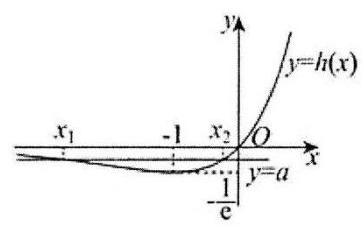
\includegraphics[max width=0.3\textwidth]{images/bo_d5jma53ef24c73bll4ig_50_296_425_364_227_0.jpg}
\end{center}
\hspace*{3em} 

当 \(- \frac{1}{\mathrm{e}} < a < 0\) 时,直线 \(y = a\) 与 \(y = h\left( x\right)\) 的图象有 2 个交点,

设这两个交点的横坐标分别为 \({x}_{1}\text{ 、 }{x}_{2}\) ,且 \({x}_{1} < {x}_{2}\) ,

当 \(x < {x}_{1}\) 或 \(x > {x}_{2}\) 时, \({f}^{\prime }\left( x\right)  = x{e}^{x} - a > 0\) ,

当 \({x}_{1} < x < {x}_{2}\) 时, \({f}^{\prime }\left( x\right)  = x{e}^{x} - a < 0\) ,此时函数有 2 个极值点,

所以 \(a\) 的取值范围是 \(\left( {-\frac{1}{\mathrm{e}},0}\right)\)

【练习】8. (2025 届复附) 已知函数 \(f\left( x\right)  = \left| {x - a}\right| ,g\left( x\right)  = {x}^{2} + {2ax} + l\left( {a\text{ 为正常数 }}\right)\) ,且函数 \(y = f\left( x\right)\) 与 \(y = g\left( x\right)\) 的图象在 \(y\) 轴上的截距相等. 记 \(h\left( x\right)  = f\left( x\right)  + b\sqrt{g\left( x\right) }\) ,其中 \(b\) 为常数

(1)讨论函数 \(y = h\left( x\right)\) 的奇偶性;

(2)若 \(h\left( x\right)  \geq  2\) 恒成立，求 \(b\) 的取值范围

【解析】 \(\left( 1\right) h\left( x\right)  = f\left( x\right)  + b\sqrt{g\left( x\right) } = \left| {x - 1}\right|  + b\left| {x + 1}\right|\) ,其定义域为 \(R\) ,

所以 \(h\left( {-x}\right)  = \left| {x + 1}\right|  + b\left| {x - 1}\right|\)

若 \(h\left( x\right)\) 为偶函数，即 \(h\left( x\right)  = h\left( {-x}\right)\) ，则有 \(b = 1\) ，此时 \(h\left( 2\right)  = 4,h\left( {-2}\right)  = 4\) ，

故 \(h\left( 2\right)  \neq   - h\left( {-2}\right)\) ，即 \(h\left( x\right)\) 不为奇函数；

若 \(h\left( x\right)\) 为奇函数，即 \(h\left( x\right)  =  - h\left( {-x}\right)\) ，则 \(b =  - 1\) ，此时 \(h\left( 2\right)  = 2,h\left( {-2}\right)  =  - 2\) ，

故 \(h\left( 2\right)  \neq  h\left( {-2}\right)\) ,即 \(h\left( x\right)\) 不为偶函数;

综上,当且仅当 \(b = 1\) 时,函数 \(h\left( x\right)\) 为偶函数,且不为奇函数,

当且仅当 \(b =  - 1\) 时,函数 \(h\left( x\right)\) 为奇函数,且不为偶函数,

当 \(b \neq   \pm  1\) 时,函数 \(h\left( x\right)\) 既非奇函数又非偶函数

\(\left( 2\right) h\left( x\right)  = f\left( x\right)  + b\sqrt{g\left( x\right) } = \left| {x - 1}\right|  + b\left| {x + 1}\right|  \geq  2\) 恒成立,

由 \(h\left( 1\right)  = {2b} \geq  2\) 得 \(b \geq  1\) ,此时 \(h\left( x\right)  = \left| {x - 1}\right|  + \left| {x + 1}\right|  + \left( {b - 1}\right) \left| {x + 1}\right|  \geq  2\) ,

故 \(b \geq  1\)

【练习】9. (2025 届复附) 设 \(f\left( x\right)  = \frac{2{x}^{2}}{x + 1},g\left( x\right)  = {ax} + 5 - {2a}\left( {a > 0}\right)\)

(1)求 \(f\left( x\right)\) 在 \(x \in  \left\lbrack  {0,1}\right\rbrack\) 上的值域;

(2)若对于任意 \({x}_{1} \in  \left\lbrack  {0,1}\right\rbrack\) ，总存在 \({x}_{0} \in  \left\lbrack  {0,1}\right\rbrack\) ，使得 \(g\left( {x}_{0}\right)  = f\left( {x}_{1}\right)\) 成立，求 \(a\) 的取值范围

【解析】(1) \({f}^{\prime }\left( x\right)  = \frac{{4x}\left( {x + 1}\right)  - 2{x}^{2}}{{\left( x + 1\right) }^{2}} = \frac{2{x}^{2} + {4x}}{{\left( x + 1\right) }^{2}} \geq  0\) 在 \(x \in  \left\lbrack  {0,1}\right\rbrack\) 上恒成立

所以 \(f\left( x\right)\) 在 \(\left\lbrack  {0,1}\right\rbrack\) 上严格增,所以 \(f\left( x\right)\) 值域为 \(\left\lbrack  {0,1}\right\rbrack\)

(2) \(g\left( x\right)  = {ax} + 5 - {2a}\left( {a > 0}\right)\) 在 \(x \in  \left\lbrack  {0,1}\right\rbrack\) 上的值域 \(\left\lbrack  {5 - {2a},5 - a}\right\rbrack\)

由条件得 \(\left\lbrack  {0,1}\right\rbrack   \subseteq  \left\lbrack  {5 - {2a},5 - a}\right\rbrack\) ,所以 \(\left\{  {\begin{array}{l} 5 - {2a} \leq  0 \\  5 - a \geq  1 \end{array} \Rightarrow  \frac{5}{2} \leq  a \leq  4}\right.\)

【练习】10. 已知常数 \(a > 1\) ,函数 \(y = f\left( x\right)\) 的表达式为 \(f\left( x\right)  = {\log }_{a}\left( {x + 2}\right)  - {\log }_{a}\left( {2 - x}\right)\) .

(1)证明:函数 \(y = f\left( x\right)\) 是奇函数；

(2)若函数 \(y = f\left( x\right)\) 在区间 \(\left\lbrack  {0,1}\right\rbrack\) 上的最大值为 2，求实数 \(a\) 的值.

【解析】(1) 由 \(\left\{  \begin{array}{l} x + 2 > 0 \\  2 - x > 0 \end{array}\right.\) ,解得 \(- 2 < x < 2,\cdots \cdots 3\)

所以 \(y = f\left( x\right)\) 的 \(D = \left( {-2,2}\right)\) ,任取 \(x \in  D\) ,则 \(- x \in  D\) ,

因为 \(f\left( {-x}\right)  = {\log }_{a}\left( {-x + 2}\right)  - {\log }_{a}\left( {2 + x}\right)  =  - f\left( x\right)\) ,

所以 \(y = f\left( x\right)\) 是奇函数. \(\cdots \cdots 6\) 分

(2) 法一: 当 \(a > 1,y = {\log }_{a}\left( {x + 2}\right) ,y =  - {\log }_{a}\left( {2 - x}\right)\) 在 \(\left\lbrack  {0,1}\right\rbrack\) 上严格增,

所以 \(y = f\left( x\right)\) 在 \(\left\lbrack  {0,1}\right\rbrack\) 上严格增, \(\cdots \cdots 8\) 分

因此, \(f{\left( x\right) }_{\max } = f\left( 1\right)  = 2,\cdots \cdots {10}\) 分

即 \({\log }_{a}3 = 2,{a}^{2} = 3\) ,所以 \(a = \sqrt{3}.\cdots \cdots {14}\) 分

法二: \(f\left( x\right)  = {\log }_{a}\left( {x + 2}\right)  - {\log }_{a}\left( {2 - x}\right)  = {\log }_{a}\left( \frac{x + 2}{2 - x}\right) ,a > 1\) ,

因为 \(x \in  \left\lbrack  {0,1}\right\rbrack\) ,令 \(t = \frac{x + 2}{2 - x} = \frac{-\left( {2 - x}\right)  + 4}{2 - x} =  - 1 + \frac{4}{2 - x} \in  \left\lbrack  {1,3}\right\rbrack\) ,

又 \(a > 1\) ，所以 \(y = {\log }_{a}t\) 在 \(\left\lbrack  {1,3}\right\rbrack\) 上严格增， \(\cdots \cdots 8\) 分

因而 \(f{\left( x\right) }_{\max } = {\log }_{a}3 = 2\cdots \cdots {10}\) 分

所以 \({a}^{2} = 3,a = \sqrt{3}.\cdots \cdots {14}\) 分 2025 版上海高考真题及模拟训练合集

\section*{板块五:压轴主观题}

\section*{1. 真题回顾}

【例题】1. (2025 上海春考) 已知函数 \(y = f\left( x\right)\) 的定义域是 \(D\) . 对于 \(t \in  D\) ,定义集合 \({S}_{f\left( t\right) } =\)

\(\{ x \mid  f\left( x\right)  \geq  f\left( t\right) \} .\)

(1) \(f\left( x\right)  = {\log }_{2}x\) ,求 \({S}_{f\left( {16}\right) }\) ;

(2)对于集合 \(A\) ，若对任意 \(x \in  A\) 都有 \(- x \in  A\) ，则称 \(A\) 是对称集. 若 \(D\) 是对称集，证明: “函数 \(y \; = f\left( x\right)\) 是偶函数”的充要条件是“对任意 \(t \in  D,{S}_{f\left( t\right) }\) 是对称集”；

(3) 若 \(x \in  \mathbb{R},f\left( x\right)  = {\mathrm{e}}^{x} - \frac{1}{2}m{x}^{2}\) ,若对于任意 \({t}_{1},{t}_{2} \in  D,{t}_{1} < {t}_{2}\) ,都有 \({S}_{f\left( {t}_{2}\right) } \subseteq  {S}_{f\left( {t}_{1}\right) }\) 。求 \(m\) 的取值范围

【解析】 \(\left( 1\right) {S}_{f\left( {16}\right) } = \left\{  {x \mid  {\log }_{2}x \geq  {\log }_{2}{16}}\right\}\) ,所以 \({S}_{f\left( {16}\right) } = \lbrack {16}, + \infty )\) ;

(2)若 \(y = f\left( x\right)\) 是偶函数，则对任意 \(a \in  {S}_{f\left( t\right) }\) ，有 \(f\left( a\right)  \geq  f\left( t\right)  = f\left( {-t}\right)\) ，即 \(a \in  {S}_{f\left( {-t}\right) }\) ，于是 \({S}_{f\left( t\right) } \subseteq \; {S}_{f\left( {-t}\right) }\) ;

同理,对任意 \(b \in  {S}_{f\left( {-t}\right) }\) ,有 \(f\left( b\right)  \geq  f\left( {-t}\right)  = f\left( t\right)\) ,即 \(b \in  {S}_{f\left( t\right) }\) ,于是 \({S}_{f\left( {-t}\right) } \subseteq  {S}_{f\left( t\right) }\) ,故 \({S}_{f\left( t\right) } = {S}_{f\left( {-t}\right) }\) . 利用反证法证明命题“若对任意 \(t\) 都有 \({S}_{f\left( t\right) } = {S}_{f\left( {-t}\right) }\) ,则 \(y = f\left( x\right)\) 是偶函数”

假设 \(y = f\left( x\right)\) 不是偶函数,则存在 \({x}_{0}\) 使 \(f\left( {x}_{0}\right)  > f\left( {-{x}_{0}}\right)\) ,此时 \(- {x}_{0} \notin  {S}_{f\left( {x}_{0}\right) }\) ,但 \(- {x}_{0} \in  {S}_{f\left( {-{x}_{0}}\right) }\) ,所以 \({S}_{f\left( {x}_{0}\right) } \neq  {S}_{f\left( {-{x}_{0}}\right) }\) ,与条件矛盾,故假设错误,命题成立;

(3)显然 \({t}_{2} \in  {S}_{f\left( {t}_{2}\right) }\) ，由于 \({S}_{f\left( {t}_{2}\right) } \subseteq  {S}_{f\left( {t}_{1}\right) }\) ，所以 \({t}_{2} \in  {S}_{f\left( {t}_{1}\right) }\) ，得到 \(f\left( {t}_{2}\right)  \geq  f\left( {t}_{1}\right)\) .

另一方面,若 \(f\left( {t}_{2}\right)  \geq  f\left( {t}_{1}\right)\) ,则对任意 \(a \in  {S}_{f\left( {t}_{2}\right) },f\left( a\right)  > f\left( {t}_{2}\right)  \geq  f\left( {t}_{1}\right)\) ,所以 \(a \in  {S}_{f\left( {t}_{1}\right) }\) ,即 \({S}_{f\left( {t}_{2}\right) } \subseteq \; {S}_{f\left( {t}_{1}\right) }\) ,所以等价转化为 \(y = f\left( x\right)\) 是增函数,对 \(f\left( x\right)\) 求导得 \({f}^{\prime }\left( x\right)  = {\mathrm{e}}^{x} - {mx}\) ,则 \({f}^{\prime }\left( x\right)  \geq  0\) .

注意到 \({f}^{\prime }\left( 1\right)  = \mathrm{e} - m\) ,所以 \(m \leq  \mathrm{e}\) .

又不等式 \({\mathrm{e}}^{x} - {mx} < 0\) 在 \(m < 0\) 时有解 \(x = \frac{1}{m}\) ，所以 \(m \geq  0\) ；

另一方面,若 \(0 \leq  m \leq  \mathrm{e}\) ,在 \(x \leq  0\) 时, \({f}^{\prime }\left( x\right)  = {\mathrm{e}}^{x} - {mx}\) 显然恒正; 在 \(x > 0\) 时, \({f}^{\prime }\left( x\right)  \geq  {\mathrm{e}}^{x} - {ex}\) .

令 \(g\left( x\right)  = {\mathrm{e}}^{x} - {ex}\) ,则 \({g}^{\prime }\left( x\right)  = {\mathrm{e}}^{x} - \mathrm{e}\) ,所以 \(g\left( x\right)  = {\mathrm{e}}^{x} - {ex}\) 在 \(\left( {0,1}\right)\) 上严格减,在 \(\left( {1, + \infty }\right)\) 上严格

增,故在 \(x = 1\) 处取得最小值 \(g\left( 1\right)  = 0\) ,所以 \({f}^{\prime }\left( x\right)  = {\mathrm{e}}^{x} - {ex} \geq  0\) .

综上所述: \(m \in  \left\lbrack  {0,\mathrm{e}}\right\rbrack\) .

【例题】2. (2024 上海秋考)已知 \(D\) 是 \(R\) 的一个非空子集， \(y = f\left( x\right)\) 是定义在 \(R\) 上的函数. 对于点 \(M \; \left( {a,b}\right)\) ,函数 \(s\left( x\right)  = {\left( x - a\right) }^{2} + {\left( f\left( x\right)  - b\right) }^{2}\) . 若对于 \(P\left( {{x}_{0},f\left( {x}_{0}\right) }\right)\) ,满足 \(s\left( x\right)\) 在 \(x = {x}_{0}\) 处取得最小值,则称 \(P\) 是 \(M\) 的 \(f\) 最近点.

(1) \(D = \left( {0, + \infty }\right)\) ， \(f\left( x\right)  = \frac{1}{x}\) ， \(M\left( {0,0}\right)\) ，求证:存在 \(M\) 的 \(f\) 最近点；

(2) \(D = R,f\left( x\right)  = {\mathrm{e}}^{x},M\left( {1,0}\right)\) ,若 \(y = f\left( x\right)\) 上一点 \(P\) 满足 \({MP}\) 垂直于 \(y = f\left( x\right)\) 在 \(P\) 处的切线,则 \(P\) 是否是 \(M\) 的 \(f\) 最近点?

(3) \(D = R\) ，已知 \(y = f\left( x\right)\) 是可导的， \(y = g\left( x\right)\) 定义在 \(R\) 上且函数值恒正. 已知 \(t \in  R\) ， \({M}_{1}(t - 1\) ， \(f\left( t\right)  - g\left( t\right) ),{M}_{2}\left( {t + 1,f\left( t\right)  + g\left( t\right) }\right)\) . 若对于任意 \(t \in  R\) ,都存在 \(y = f\left( x\right)\) 上的一点 \(P\) ,使得 \(P\) 既是 \({M}_{1}\) 的 \(f\) 最近点,又是 \({M}_{2}\) 的 \(f\) 最近点. 试求 \(y = f\left( x\right)\) 的单调性.

【解析】(1) 对于点 \(M\left( {0,0}\right) ,s\left( x\right)  = {x}^{2} + {\left( \frac{1}{x}\right) }^{2} \geq  2\) ,当且仅当 \(x =  \pm  1\) 时取等号,

又 \(D = \left( {0, + \infty }\right)\) ,取 \({x}_{0} = 1\) ,所以存在 \(M\) 的 \(f\) 最近点 \(P\left( {1,1}\right)\) ;

(2) \(s\left( x\right)  = {\left( x - 1\right) }^{2} + {\mathrm{e}}^{2x}\) ,

\(f\left( x\right)  = {\mathrm{e}}^{x},{f}^{\prime }\left( x\right)  = {\mathrm{e}}^{x}\) ,设 \(P\left( {{x}_{0},{\mathrm{e}}^{{x}_{0}}}\right)\) ,

因为 \(y = f\left( x\right)\) 上一点 \(P\) 满足 \({MP}\) 垂直于 \(y = f\left( x\right)\) 在 \(P\) 处的切线,

所以 \({f}^{\prime }\left( {x}_{0}\right)  \cdot  {k}_{MP} =  - 1\) ,所以 \({\mathrm{e}}^{{x}_{0}} \cdot  \frac{{\mathrm{e}}^{{x}_{0}}}{{x}_{0} - 1} =  - 1\) ,即 \({\mathrm{e}}^{2{x}_{0}} + {x}_{0} - 1 = 0\) ,

对于 \(s\left( x\right)  = {\left( x - 1\right) }^{2} + {\mathrm{e}}^{2x},{s}^{\prime }\left( x\right)  = 2\left( {x - 1}\right)  + 2{\mathrm{e}}^{2x} = 2\left( {{\mathrm{e}}^{2x} + x - 1}\right)\) ,

则 \({s}^{\prime }\left( {x}_{0}\right)  = 0\) ,易得 \({s}^{\prime }\left( x\right)\) 严格增,

则当 \(x < {x}_{0}\) 时， \({s}^{\prime }\left( x\right)  < 0\) ， \(s\left( x\right)\) 严格减，

当 \(x > {x}_{0}\) 时， \({s}^{\prime }\left( x\right)  > 0\) ， \(s\left( x\right)\) 严格增，

故 \(s\left( x\right)\) 在 \(x = {x}_{0}\) 处取得最小值，则 \(P\) 是 \(M\) 的 \(f\) 最近点；

(3) \({S}_{{M}_{1}}\left( x\right)  = {\left( x - t + 1\right) }^{2} + {\left( f\left( x\right)  - f\left( t\right)  + g\left( t\right) \right) }^{2}\) ,

\({S}_{{M}_{2}}\left( x\right)  = {\left( x - t - 1\right) }^{2} + {\left( f\left( x\right)  - f\left( t\right)  - g\left( t\right) \right) }^{2},\)

则 \({S}_{{M}_{1}^{\prime }}\left( x\right)  = 2\left( {x - t + 1}\right)  + 2\left( {f\left( x\right)  - f\left( t\right)  + g\left( t\right) }\right)  \cdot  {f}^{\prime }\left( x\right)\) ,

\({S}_{{M}_{2}^{\prime }}\left( x\right)  = 2\left( {x - t - 1}\right)  + 2\left( {f\left( x\right)  - f\left( t\right)  - g\left( t\right) }\right)  \cdot  {f}^{\prime }\left( x\right) ,\)

若对于任意 \(t \in  R\) ,都存在 \(y = f\left( x\right)\) 上的一点 \(P\) ,

使得 \(P\) 既是 \({M}_{1}\) 的 \(f\) 最近点,又是 \({M}_{2}\) 的 \(f\) 最近点,

则存在 \({x}_{0}\) ,使得 \({S}_{{M}_{1}^{\prime }}\left( {x}_{0}\right)  = {S}_{{M}_{2}^{\prime }}\left( {x}_{0}\right)  = 0\) ,

则 \({S}_{{M}_{1}^{\prime }}\left( {x}_{0}\right)  - {S}_{{M}_{2}^{\prime }}\left( {x}_{0}\right)  = 0\) ,即 \(4 + {4g}\left( t\right)  \cdot  {f}^{\prime }\left( {x}_{0}\right)  = 0\) ,所以 \({f}^{\prime }\left( {x}_{0}\right)  =  - \frac{1}{g\left( t\right) }\) ,

因为 \(y = g\left( x\right)\) 定义在 \(R\) 上且函数值恒正,所以 \({f}^{\prime }\left( {x}_{0}\right)  =  - \frac{1}{g\left( t\right) } < 0\left( *\right)\) ,

因为 \(P\) 既是 \({M}_{1}\) 的 \(f\) 最近点,又是 \({M}_{2}\) 的 \(f\) 最近点,

所以 \({S}_{{M}_{1}}\left( {x}_{0}\right)  = {\left( {x}_{0} - t + 1\right) }^{2} + {\left( f\left( {x}_{0}\right)  - f\left( t\right)  + g\left( t\right) \right) }^{2}\)

\(\leq  {S}_{{M}_{1}}\left( x\right)  = {\left( x - t + 1\right) }^{2} + {\left( f\left( x\right)  - f\left( t\right)  + g\left( t\right) \right) }^{2}\)  \circled{1} ,

且 \({S}_{{M}_{2}}\left( {x}_{0}\right)  = {\left( {x}_{0} - t - 1\right) }^{2} + {\left( f\left( {x}_{0}\right)  - f\left( t\right)  - g\left( t\right) \right) }^{2}\)

\(\leq  {S}_{{M}_{2}}\left( x\right)  = {\left( x - t - 1\right) }^{2} + {\left( f\left( x\right)  - f\left( t\right)  - g\left( t\right) \right) }^{2}\)  \circled{2} 恒成立，

在 \circled{1}  \circled{2} 中，令 \(x = t\) ，

得 \({S}_{{M}_{1}}\left( {x}_{0}\right)  = {\left( {x}_{0} - t + 1\right) }^{2} + {\left( f\left( {x}_{0}\right)  - f\left( t\right)  + g\left( t\right) \right) }^{2} \leq  1 + {g}^{2}\left( t\right)\) ,

即 \({\left( {x}_{0} - t\right) }^{2} + 2\left( {{x}_{0} - t}\right)  + {\left( f\left( {x}_{0}\right)  - f\left( t\right) \right) }^{2} + 2\left( {f\left( {x}_{0}\right)  - f\left( t\right) }\right)  \leq  0\)  \circled{3} ,

同理 \({\left( {x}_{0} - t\right) }^{2} - 2\left( {{x}_{0} - t}\right)  + {\left( f\left( {x}_{0}\right)  - f\left( t\right) \right) }^{2} - 2\left( {f\left( {x}_{0}\right)  - f\left( t\right) }\right)  \leq  0\)  \circled{4} ,

由 \circled{3}  \circled{4} 相加，得 \(2{\left( {x}_{0} - t\right) }^{2} + 2{\left( f\left( {x}_{0}\right)  - f\left( t\right) \right) }^{2} \leq  0\) ,

即 \({\left( {x}_{0} - t\right) }^{2} + {\left( f\left( {x}_{0}\right)  - f\left( t\right) \right) }^{2} \leq  0\) ,即 \({x}_{0} = t\) ,代入 (*) 得 \({f}^{\prime }\left( t\right)  =  - \frac{1}{g\left( t\right) } < 0\) ,

由于 \(t \in  R\) ,由 \(t\) 的任意性得 \({f}^{\prime }\left( t\right)  < 0\) 对任意 \(t\) 都成立,

则 \(y = f\left( x\right)\) 严格减.

【例题】3. (2024 上海春考)对于定义在 \(R\) 上的函数 \(f\left( x\right)\) ，记集合 \({M}_{a} = \{ t \mid  t = f\left( x\right)  - f\left( a\right) ,x \geq  a\}\) ，

\({L}_{a} = \{ t \mid  t = f\left( x\right)  - f\left( a\right) ,x \leq  a\} .\)

(1) 若 \(f\left( x\right)  = {x}^{2} + 1\) ，求 \({M}_{1}\) 和 \({L}_{1}\) ；

(2)若 \(f\left( x\right)  = {x}^{3} - 3{x}^{2}\) ，求证:对于任意 \(a \in  R\) ，都有 \({M}_{a} \subseteq  \lbrack  - 4\) ，+0 \()\) ，且存在 \(a\) ，使得 -4 ∈ \({M}_{a}\) .

(3)已知定义在 \(R\) 上的函数 \(f\left( x\right)\) 有最小值，求证: “ \(f\left( x\right)\) 是偶函数”的充要条件为“对任意 \(c >\) 0,都有 \({M}_{-c} = {L}_{c}\) ”.

【解析】(1) \(f\left( 1\right)  = 2,f\left( x\right)  - f\left( 1\right)  = {x}^{2} - 1\) ,

\({M}_{1} = \{ t \mid  t = {x}^{2} - 1,x \geq  1\}  = \lbrack 0, + \infty ),{L}_{1} = \left\{  {t \mid  t = {x}^{2} - 1,x \leq  1}\right\}   = \lbrack  - 1, + \infty )\) ;

(2) 原题即证 \(f\left( x\right)  - f\left( a\right)  = {x}^{3} - 3{x}^{2} - {a}^{3} + 3{a}^{2} \geq   - 4\) ,

令 \(g\left( x\right)  = {x}^{3} - 3{x}^{2} - {a}^{3} + 3{a}^{2}\) ,则 \({g}^{\prime }\left( x\right)  = 3{x}^{2} - {6x} = {3x}\left( {x - 2}\right)\) ,

若 \(a \geq  2,x \geq  a\) 时函数严格增, \(g\left( x\right)  \geq  g\left( a\right)  = 0\) ,即 \({M}_{a} = \lbrack 0, + \infty ) \subseteq  \lbrack  - 4, + \infty )\) ;

若 \(0 \leq  a < 2,x \geq  a\) 先减后增, \(g{\left( x\right) }_{\min } = g\left( 2\right)  =  - {a}^{3} + 3{a}^{2} - 4\) ,

因为 \(- {a}^{3} + 3{a}^{2} = {a}^{2}\left( {3 - a}\right)  \geq  0, - {a}^{3} + 3{a}^{2} - 4 \geq   - 4\) ,

所以 \({M}_{a} = \left\lbrack  {-{a}^{3} + 3{a}^{2} - 4, + \infty }\right)  \subseteq  \left\lbrack  {-4, + \infty }\right)\) ; 且当 \(a = 0\) 时, \({M}_{a} = \left\lbrack  {-4, + \infty }\right)\) ;

若 \(a < 0\) ，函数在 \(\lbrack a,0)\) 严格增，在 \(\left\lbrack  {0,2}\right\rbrack\) 严格减，在 \(\lbrack 2, + \infty )\) 严格增，

所以 \(g{\left( x\right) }_{\min } = \min \{ g\left( a\right) ,g\left( 2\right) \}  = \min \left\{  {0, - {a}^{3} + 3{a}^{2} - 4}\right\}\) ,

当 \(a < 0\) 时，因为 \(- {a}^{3} + 3{a}^{2} = {a}^{2}\left( {3 - a}\right)  > 0, - {a}^{3} + 3{a}^{2} - 4 >  - 4\) ，

此时 \({M}_{a} = \left\lbrack  {g{\left( x\right) }_{\min }, + \infty }\right)  \subseteq  \left\lbrack  {-4, + \infty }\right)\) ;

综上,对于任意 \(a \in  R\) ,都有 \({M}_{a} \subseteq  \lbrack  - 4, + \infty )\) ,且存在 \(a = 0\) ,使得 \(- 4 \in  {M}_{a}\) ;

(3)必要性

因为 \(f\left( x\right)\) 是偶函数，

任意 \(t \in  {M}_{-c}\) ,必有 \(x \in  \lbrack  - c, + \infty )\) ,使得 \(t = f\left( x\right)  - f\left( {-c}\right)  = f\left( {-x}\right)  - f\left( c\right)\) ,

又 \(- x \in  ( - \infty ,c\rbrack\) ,所以 \(t \in  {L}_{c}\) . 因此 \({M}_{-c} \subseteq  {L}_{c}\) .

任意 \(t \in  {L}_{c}\) ,必有 \(x \in  ( - \infty ,c\rbrack\) ,使得 \(t = f\left( x\right)  - f\left( c\right)  = f\left( {-x}\right)  - f\left( {-c}\right)\) ,

又 \(- x \in  \lbrack  - c, + \infty )\) ,所以 \(t \in  {M}_{-c}\) . 因此 \({L}_{c} \subseteq  {M}_{-c}\) .

综上,对任意 \(c \in  R,{M}_{-c} = {L}_{c}\) .

充分性

任意 \(c \in  R,{M}_{-c} = {L}_{c}\) ,不妨设 \(f\left( x\right)\) 在 \(x = m\) 处取得最小值,

即 \(f{\left( x\right) }_{\min } = f\left( m\right)  = k,M\) 取右侧, \(L\) 取左侧,

当 \(x \geq  m\) 时, \(f\left( x\right)  \geq  f\left( m\right)  = k\) ,

所以 \(t = f\left( x\right)  - f\left( a\right)  \geq  f\left( x\right)  - f\left( m\right)  \geq  0\) ,

又 \({M}_{m} = {L}_{-m}\) ,所以在 \({M}_{m} = {L}_{-m},\therefore {L}_{-m}\) 中,当 \(x \leq   - m\) 时, \(t = f\left( x\right)  - f\left( {-m}\right)  \geq  0\) ,

同理,任意 \(x \leq  m,{L}_{m}\) 非负, \({M}_{-m}\) 中,当 \(x \geq   - m\) 时, \(t = f\left( x\right)  - f\left( {-m}\right)  \geq  0\) ,

所以任意 \(x \in  R,f\left( x\right)  \geq  f\left( {-m}\right)\) ,

即 \(f\left( m\right)  = f\left( {-m}\right)  = k\) ,即 \(- m\) 也是 \(f\left( x\right)\) 的最小值点,

接下来证明 \(f\left( x\right)  = f\left( {-x}\right)\) 对于任意 \(x \in  R\) 恒成立,

当 \({x}_{0} \geq  0\) 时, \({M}_{-{x}_{0}} = {L}_{{x}_{0}}\) ,

\(\left| m\right|  \geq   - {x}_{0},f\left( \left| m\right| \right)  - f\left( {-{x}_{0}}\right)  \in  {M}_{-{x}_{0}},\)

\(- \left| m\right|  \leq  {x}_{0},f\left( {-\left| m\right| }\right)  - f\left( {x}_{0}\right)  \in  {L}_{{x}_{0}},\)

\(f\left( \left| m\right| \right)\) 和 \(f\left( {-\left| m\right| }\right)\) 均为最小值,

所以 \({M}_{-{x}_{0}}\) 中最小值为 \(f\left( \left| m\right| \right)  - f\left( {-{x}_{0}}\right) ,{L}_{{x}_{0}}\) 中最小值为 \(f\left( {-\left| m\right| }\right)  - f\left( {x}_{0}\right)\) ,

因为 \({M}_{-{x}_{0}} = {L}_{{x}_{0}}\) ,所以 \(f\left( {-{x}_{0}}\right)  = f\left( {x}_{0}\right)\) 对 \({x}_{0} \geq  0\) 恒成立,

所以 \(f\left( x\right)\) 是偶函数.

证毕.

【例题】4. (2023 上海春考) 设函数 \(f\left( x\right)  = a{x}^{3} - \left( {a + 1}\right) {x}^{2} + x,g\left( x\right)  = {kx} + m\) ,其中 \(a \geq  0,k,m \in  R\) ,若任意 \(x \in  \left\lbrack  {0,1}\right\rbrack\) 均有 \(f\left( x\right)  \leq  g\left( x\right)\) ,则称函数 \(y = g\left( x\right)\) 是函数 \(y = f\left( x\right)\) 的“控制函数”,且对所有的函数 \(y = g\left( x\right)\) 取最小值定义为 \(\bar{f}\left( x\right)\) .

(1) 若 \(a = 2,g\left( x\right)  = x\) ,试问 \(y = g\left( x\right)\) 是否为函数 \(y = f\left( x\right)\) 的“控制函数”;

(2) 若 \(a = 0\) ，使得直线 \(y = h\left( x\right)\) 是曲线 \(y = f\left( x\right)\) 在 \(x = \frac{1}{4}\) 处的切线. 证明:函数 \(y = h\left( x\right)\) 为函数 \(y = f\left( x\right)\) 的“控制函数”,并求 \(\bar{f}\left( \frac{1}{4}\right)\) 的值;

(3) 若曲线 \(y = f\left( x\right)\) 在 \(x = {x}_{0}\left( {{x}_{0} \in  \left( {0,1}\right) }\right)\) 处的切线过点 \(\left( {1,0}\right)\) ,且 \(c \in  \left\lbrack  {0,1}\right\rbrack\) . 证明: 当且仅当 \(c \; = {x}_{0}\) 或 \(c = 1\) 时, \(\bar{f}\left( c\right)  = f\left( c\right)\) .

【解析】(1) 若 \(a = 2,f\left( x\right)  = 2{x}^{3} - 3{x}^{2} + x,g\left( x\right)  = x\) ,

\(f\left( x\right)  - g\left( x\right)  = 2{x}^{3} - 3{x}^{2}\) ,令 \(h\left( x\right)  = 2{x}^{3} - 3{x}^{2},x \in  \left\lbrack  {0,1}\right\rbrack\) ,

令 \({h}^{\prime }\left( x\right)  = 6{x}^{2} - {6x} = {6x}\left( {x - 1}\right)  \leq  0\) ,得 \(x \in  \left\lbrack  {0,1}\right\rbrack\) ,

所以 \({h}^{\prime }\left( x\right)  = 6{x}^{2} - {6x} = {6x}\left( {x - 1}\right)  \leq  0 \Rightarrow  x \in  \left\lbrack  {0,1}\right\rbrack  ,\therefore h\left( x\right)\) 在 \(\left\lbrack  {0,1}\right\rbrack\) 严格减，所以 \(\left\lbrack  {0,1}\right\rbrack   \searrow  ;{h}_{\max } \; \left( x\right)  = h\left( 0\right)  = 0,\)

所以 \(f\left( x\right)  - g\left( x\right)  \leq  h{\left( x\right) }_{\max } = 0\) ，所以 \(g\left( x\right)\) 是 \(f\left( x\right)\) 的 “控制函数”；

(2) 若 \(a = 0,f\left( x\right)  =  - {x}^{2} + x,f\left( \frac{1}{4}\right)  = \frac{3}{16},{f}^{\prime }\left( x\right)  =  - {2x} + 1,{f}^{\prime }\left( \frac{1}{4}\right)  =  - \frac{1}{2} + 1 = \frac{1}{2}\) ,

所以 \(h\left( x\right)  = \frac{1}{2}\left( {x - \frac{1}{4}}\right)  + \frac{3}{16}\) ,即 \(h\left( x\right)  = \frac{1}{2}x + \frac{1}{16}\) ,

\(f\left( x\right)  - g\left( x\right)  =  - {\left( x - \frac{1}{4}\right) }^{2} \leq  0\) 恒成立，所以 \(h\left( x\right)\) 是 \(f\left( x\right)\) 的“控制函数”；

法一: \(f\left( \frac{1}{4}\right)  = h\left( \frac{1}{4}\right)  = \frac{3}{16}\) ,又 \(g\left( \frac{1}{4}\right)  \geq  f\left( \frac{1}{4}\right)  = \frac{3}{16}\) ,所以 \(\bar{f}\left( \frac{1}{4}\right)  = \frac{3}{16}\) .

法二: 设抛物线上点 \(\left( {{x}_{0}, - {x}_{0}^{2} + {x}_{0}}\right) ,{x}_{0} \in  \left\lbrack  {0,1}\right\rbrack  ,{f}^{\prime }\left( {x}_{0}\right)  =  - 2{x}_{0} + 1\) ,

有切线方程 \(y = \left( {-2{x}_{0} + 1}\right) \left( {x - {x}_{0}}\right)  - {x}_{0}^{2} + {x}_{0}\) ,

所以 \(y = \left( {-2{x}_{0} + 1}\right) \left( {\frac{1}{4} - {x}_{0}}\right)  - {x}_{0}^{2} + {x}_{0}\) ,

化简得 \(y = {x}_{0}^{2} - \frac{{x}_{0}}{2} + \frac{1}{4} = {\left( {x}_{0} - \frac{1}{4}\right) }^{2} + \frac{3}{16}\) ,最小值为 \(\frac{3}{16}\) .

(3) 法一: \(f\left( x\right)  = a{x}^{3} - \left( {a + 1}\right) {x}^{2} + x,{f}^{\prime }\left( x\right)  = {3a}{x}^{2} - 2\left( {a + 1}\right) x + 1\) ,

设 \(x = {x}_{0}\) 处的切线为 \(t\left( x\right)\) ,则 \(t\left( x\right)  = {f}^{\prime }\left( {x}_{0}\right) \left( {x - x}\right)  + f\left( {x}_{0}\right)\) ,

显然 \(t\left( {x}_{0}\right)  = f\left( {x}_{0}\right)  \cdot  t\left( x\right)\) 过点 \(\left( {1,0}\right)  \Rightarrow  t\left( 1\right)  = 0 = f\left( 1\right)\) ,

\({f}^{\prime }\left( {x}_{0}\right)  = {3a}{x}_{0}^{2} - 2\left( {a + 1}\right) {x}_{0} + 1 \Rightarrow  {f}^{\prime }\left( {x}_{0}\right) \left( {1 - {x}_{0}}\right)  = f\left( 1\right)  - f\left( {x}_{0}\right)\)

\(= \left( {1 - {x}_{0}}\right) \left\lbrack  {a\left( {\left( {1 + {x}_{0} + {x}_{0}^{2}}\right)  - \left( {a + 1}\right) \left( {1 - {x}_{0}}\right)  + 1}\right)  + 1}\right\rbrack  ,\)

所以 \({3a}{x}_{0}^{2} - 2\left( {a + 1}\right) {x}_{0} + 1 = a{x}_{0}^{2} - {x}_{0} \Rightarrow  \left( {{2a}{x}_{0} - 1}\right) \left( {{x}_{0} - 1}\right)  = 0\) ,

因为 \({x}_{0} \neq  1\) ，所以 \(a = \frac{1}{2{x}_{0}} \in  \left( {\frac{1}{2}, + \infty }\right)\) ，所以 \({x}_{0} = \frac{1}{2a}\) ，

\({f}^{\prime }\left( {x}_{0}\right)  = {3a}{\left( \frac{1}{2a}\right) }^{2} - 2\left( {a + 1}\right) \frac{1}{2a} + 1 =  - \frac{1}{4a},\)

\(f\left( {x}_{0}\right)  = a{\left( \frac{1}{2a}\right) }^{3} - \left( {a + 1}\right) {\left( \frac{1}{2a}\right) }^{2} + \frac{1}{2a} = \frac{{2a} - 1}{8{a}^{2}},\)

所以 \(t\left( x\right)  = {f}^{\prime }\left( {x}_{0}\right) \left( {x - {x}_{0}}\right)  + f\left( {x}_{0}\right)  =  - \frac{1}{4a}\left( {x - \frac{1}{2a}}\right)  + \frac{{2a} - 1}{8{a}^{2}}\) ,

即 \(t\left( x\right)  =  - \frac{1}{4a}\left( {x - 1}\right)\) ,又因为 \(f\left( x\right)  = x\left( {x - 1}\right) \left( {{ax} - 1}\right)  \leq  t\left( x\right)\)

\(\Rightarrow  a{x}^{2} - x + \frac{1}{4a} \geq  0\) 即 \(\left( {x - \frac{1}{2a}}\right)  \geq  0\) 恒成立,

所以 \(t\left( x\right)\) 必为 \(f\left( x\right)\) 的“控制函数”;

又因为任意 \(g\left( x\right)  = {kx} + m \geq  f\left( x\right)\) ,

所以任意 \(\bar{f}\left( x\right)  \geq  f\left( x\right) ,\bar{f}\left( x\right)  = f\left( x\right) ,x \in  \left( {0,1}\right)\) ,

此时 “控制函数” \(g\left( x\right)\) 必与 \(f\left( x\right)\) 切于 \(x\) 点, \(t\left( x\right)\) 与 \(f\left( x\right)\) 在 \(x = \frac{1}{2a}\) 处相切, 过 \(\left( {1,0}\right)\) ,所以在 \(\left( {\frac{1}{2a},1}\right)\) 之间点不可能使 \(f\left( x\right)\) 在 \(\left( {\frac{1}{2a},1}\right)\) 切线下方,

所以 \(\bar{f}\left( c\right)  = f\left( c\right)  \Rightarrow  c = \frac{1}{2a} = {x}_{0}\) 或 1,

故当且仅当 \(c = {x}_{0}\) 或 \(c = 1\) 时, \(\bar{f}\left( c\right)  = f\left( c\right)\) .

法二: 因为 \(f\left( x\right)  = a{x}^{3} - \left( {a + 1}\right) {x}^{2} + x\) ,所以 \({f}^{\prime }\left( x\right)  = {3a}{x}^{2} - 2\left( {a + 1}\right) x + 1\) ,

设点 \(\left( {{x}_{0},f\left( {x}_{0}\right) }\right)\) 处的切线方程为 \(y = {f}^{\prime }\left( {x}_{0}\right) \left( {x - {x}_{0}}\right)  + f\left( {x}_{0}\right)\) ,

因为直线过 \(\left( {1,0}\right)\) ,所以 \(0 = {f}^{\prime }\left( {x}_{0}\right) \left( {1 - {x}_{0}}\right)  + f\left( {x}_{0}\right)\) ,

得 \(\left\lbrack  {{3a}{x}_{0}^{2} - 2\left( {a + 1}\right) {x}_{0} + 1}\right\rbrack  \left( {1 - {x}_{0}}\right)  + a{x}_{0}^{3} - \left( {a + 1}\right) {x}_{0}^{2} + {x}_{0} = 0\) ,

化简得 \(- {2a}{x}_{0}{\left( {x}_{0} - 1\right) }^{2} + {\left( {x}_{0} - 1\right) }^{2} = 0\) ,因为 \({x}_{0} \in  \left( {0,1}\right)\) ,所以 \({\left( {x}_{0} - 1\right) }^{2} \neq  0\) ,

故 \(- {2a}{x}_{0} + 1 = 0\) ,即 \(a = \frac{1}{2{x}_{0}},a \neq  0\) .

所以 \({f}^{\prime }\left( {x}_{0}\right)  =  - \frac{{x}_{0}}{2}\) ,所以 \(y =  - \frac{{x}_{0}}{2}\left( {x - 1}\right)\) ,

设 \(\varphi \left( x\right)  = g\left( x\right)  - f\left( x\right)  =  - \frac{{x}_{0}}{2}\left( {x - 1}\right)  - a{x}^{3} + \left( {a + 1}\right) {x}^{2} - x\) ,

有 \({\varphi }^{\prime }\left( x\right)  =  - \frac{{x}_{0}}{2} - {3a}{x}^{2} + 2\left( {a + 1}\right) x - 1\) ,

令 \({\varphi }^{\prime }\left( x\right)  = 0\) ,即 \(3{x}^{2} - \left( {2 + 4{x}_{0}}\right) x + {x}_{0}\left( {{x}_{0} + 2}\right)  = 0\) ,

得 \(\left\lbrack  {{3x} - \left( {{x}_{0} + 2}\right) }\right\rbrack  \left\lbrack  {x - {x}_{0}}\right\rbrack   = 0\) ,解得 \({x}_{1} = {x}_{0},{x}_{2} = \frac{{x}_{0} + 2}{3}\) ,

可以算得 \({x}_{0} < \frac{{x}_{0} + 2}{3}\) ,

当 \(x \in  \left( {{x}_{0},\frac{{x}_{0} + 2}{3}}\right)\) 时, \({\varphi }^{\prime }\left( x\right)  > 0\) ,所以 \(\varphi \left( x\right)\) 严格增;

当 \(x \in  \left( {\frac{{x}_{0} + 2}{3},1}\right)\) 时, \({\varphi }^{\prime }\left( x\right)  < 0\) ,所以 \(\varphi \left( x\right)\) 严格减;

所以在 \(\varphi \left( {x}_{0}\right)\) 或 \(\varphi \left( 1\right)\) 处取最小值.

又因为 \(\varphi \left( {x}_{0}\right)  = \varphi \left( 1\right)  = 0\) ,所以有 \(\varphi \left( x\right)  \geq  0\) ,所以有 \(g\left( x\right)  \geq  f\left( x\right)\) .

所以在端点 \(c = {x}_{0}\) 或者 \(c = 1\) 处取得最小值.

即当且仅当 \(c = {x}_{0}\) 或 \(c = 1\) 时, \(\bar{f}\left( c\right)  = f\left( c\right)\) .

法三: \(f\left( x\right)  = x\left( {1 - {ax}}\right) \left( {1 - x}\right) ,{f}^{\prime }\left( x\right)  = {3a}{x}^{2} - 2\left( {a + 1}\right) x + 1\) ,

\(\frac{f\left( {x}_{0}\right)  - 0}{{x}_{0} - 1} = {x}_{0}\left( {a{x}_{0} - 1}\right)\) ,由于是切线,该值等于 \({f}^{\prime }\left( {x}_{0}\right)\) ,

所以 \({3a}{x}_{0}^{2} - 2\left( {a + 1}\right) {x}_{0} + 1 = a{x}_{0}^{2} - {x}_{0}\) ,整理得 \(\left( {{2a}{x}_{0} - 1}\right) \left( {{x}_{0} - 1}\right)  = 0\) ,

考虑到 \({x}_{0} \in  \left( {0,1}\right)\) ,所以 \({x}_{0} = \frac{1}{2a}\) ,所以 \(a \in  \left( {\frac{1}{2}, + \infty }\right)\) ,

\({x}_{0}\) 处的切线方程所代表的函数 \(g\left( x\right)  = \left( {x - {x}_{0}}\right) {x}_{0}\left( {a{x}_{0} - 1}\right)  + f\left( {x}_{0}\right)\) ,

一方面,对任意 \(x \in  \left( {{x}_{0},1}\right)\) ,必有 \(\bar{f}\left( x\right)  \geq  g\left( x\right)\) ,

否则若存在 \(x \in  \left( {{x}_{0},1}\right) ,\bar{f}\left( x\right)  < g\left( x\right)\) ,考虑到 \(\bar{f}\left( {x}_{0}\right)  \geq  f\left( {x}_{0}\right)\) ,

所以过 \(\left( {x,\bar{f}\left( x\right) }\right)\) 的“控制函数”的斜率 \(k < {x}_{0}\left( {a{x}_{0} - 1}\right)\) ,

考虑到 \(\bar{f}\left( 1\right)  \geq  f\left( 1\right)  = 0\) ,

所以过 \(\left( {x,\bar{f}\left( x\right) }\right)\) 的 “控制函数” 的斜率 \(k > {x}_{0}\left( {a{x}_{0} - 1}\right)\) ,两者矛盾!

另一方面,记 \(k\left( x\right)  = g\left( x\right)  - f\left( x\right)\) ,

\({k}^{\prime }\left( x\right)  = {x}_{0}\left( {a{x}_{0} - 1}\right)  = {3a}{x}^{2} + 2\left( {a + 1}\right) x - 1,\)

计算得 \(k\left( {x}_{0}\right)  = k\left( 1\right)  = 0,{k}^{\prime }\left( {x}_{0}\right)  = 0\) ,由于 \(a > \frac{1}{2}\) ,

所以 \({k}^{\prime }\left( x\right)\) 的图像为开口向下的二次函数,其对称轴为 \(x = \frac{a + 1}{3a}\) ,

注意到 \(\frac{a + 1}{3a} - \frac{1}{2a} = \frac{{2a} - 1}{6a} > 0\) ,即 \({x}_{0}\) 在对称轴左边,

设 \({k}^{\prime }\left( x\right)\) 的另一个零点为 \({x}_{1}\) ,

\({k}^{\prime }\left( x\right)\) 在 \(\left( {0,{x}_{0}}\right)\) 上为负,在 \(\left( {{x}_{0},{x}_{1}}\right)\) 上为正,在 \(\left( {{x}_{1}, + \infty }\right)\) 上为负,

即 \(k\left( x\right)\) 在 \(\left\lbrack  {0,{x}_{0}}\right\rbrack\) 上严格减，在 \(\left\lbrack  {{x}_{0},{x}_{1}}\right\rbrack\) 上严格增，在 \(\left\lbrack  {{x}_{1}, + \infty }\right)\) 上严格减，

考虑到 \(k\left( {x}_{0}\right)  = 0\) 与 \(k\left( 1\right)  = 0\) ,则必有 \({x}_{1} \in  \left( {{x}_{0},1}\right)\) ,

且当 \(x \in  \left\lbrack  {0,1}\right\rbrack\) 时, \(k\left( x\right)  \geq  0\) ,即 \(g\left( x\right)\) 是 \(f\left( x\right)\) 的“控制函数”,

及当 \(c \in  \left\lbrack  {{x}_{0},1}\right\rbrack\) 时， \(k\left( c\right)  \geq  0\) ，等号当且仅当 \(c = {x}_{0}\) 或 \(c = 1\) ，

综上,对 \(c \in  \left\lbrack  {{x}_{0},1}\right\rbrack\) ,仅在 \(c = {x}_{0}\) 或 \(c = 1\) 时, \(\bar{f}\left( x\right)  = f\left( x\right)\) ,

\(c \in  \left( {{x}_{0},1}\right)\) 时, \(\bar{f}\left( x\right)  \geq  g\left( x\right)  > f\left( x\right)\) ,命题得证.

【例题】5. (2022 上海春考) 在定义域为 \(\mathbb{R}\) 的函数 \(f\left( x\right)\) 上,定义下面两个变换: 甲变换: \(f\left( x\right)  \rightarrow  f\left( x\right)  - \; f\left( {x - t}\right)\) ,乙变换: \(f\left( x\right)  \rightarrow  \left| {f\left( {x + t}\right)  - f\left( x\right) }\right|\) ,其中 \(t > 0\) .

(1) 若 \(t = 1,f\left( x\right)  = {2}^{x}\) ,对 \(f\left( x\right)\) 进行甲变换后得到函数 \(g\left( x\right)\) ,求方程 \(g\left( x\right)  = 2\) 的解;

( 2 )若 \(f\left( x\right)  = {x}^{2}\) ，对 \(f\left( x\right)\) 进行乙变换后得到函数 \(h\left( x\right)\) ，解不等式: \(h\left( x\right)  \leq  f\left( x\right)\) ；

(3)已知定义 \(\mathbb{R}\) 上的函数 \(f\left( x\right)\) 在 \(\left( {-\infty ,0}\right)\) 单调递增，在对函数 \(f\left( x\right)\) 先作甲变换得到 \(u\left( x\right)\) ，再作乙变换得到函数 \({h}_{1}\left( x\right)\) ,对函数 \(f\left( x\right)\) 先作乙变换得到 \(v\left( x\right)\) ,再作甲变换得到函数 \({h}_{2}\left( x\right)\) ,且对于任意 \(t > 0\) ，在 \(\mathbb{R}\) 上有 \({h}_{1}\left( x\right)  = {h}_{2}\left( x\right)\) 成立，证明:函数 \(f\left( x\right)\) 在 \(\mathbb{R}\) 上单调递增.

【解析】(1) 由题意得 \(g\left( x\right)  = {2}^{x} - {2}^{x - 1} = {2}^{x - 1} = 2\) ,故 \(x = 2\) ;

(2) 由题意得 \(h\left( x\right)  = \left| {{\left( x + t\right) }^{2} - {x}^{2}}\right|  = \left| {{2tx} + {t}^{2}}\right|  \leq  f\left( x\right)  = {x}^{2},t > 0\) ,

法一: 当 \(x \leq   - \frac{t}{2}\) 时, \(- {2tx} - {t}^{2} \leq  {x}^{2}\) ,即 \({\left( x + t\right) }^{2} \geq  0\) ,故 \(x \leq   - \frac{t}{2}\) ;

当 \(x \geq   - \frac{t}{2}\) 时, \({2tx} + {t}^{2} \leq  {x}^{2}\) ,即 \({x}^{2} - {2tx} - {t}^{2} \geq  0\) ,

解得 \(x \in  \left( {-\infty ,\left( {1 - \sqrt{2}}\right) t}\right\rbrack   \cup  \lbrack \left( {1 + \sqrt{2}}\right) t, + \infty )\) ,

所以 \(x \in  \left( {-\frac{t}{2},\left( {1 - \sqrt{2}}\right) t}\right\rbrack   \cup  \left\lbrack  {\left( {1 + \sqrt{2}}\right) t, + \infty }\right)\) ;

综上,解集为 \(x \in  \left( {-\infty ,\left( {1 - \sqrt{2}}\right) t\rbrack \cup \lbrack \left( {1 + \sqrt{2}}\right) t, + \infty }\right)\) ;

法二: \(\left| {{2tx} + {t}^{2}}\right|  \leq  {x}^{2} \Rightarrow   - {x}^{2} \leq  {2tx} + {t}^{2} \leq  {x}^{2}\) ,

即 \(\left\{  \begin{array}{l} {x}^{2} + {2tx} + {t}^{2} \geq  0 \\  {x}^{2} - {2tx} - {t}^{2} \geq  0 \end{array}\right.\) ,解得 \(x \in  \left( {-\infty ,\left( {1 - \sqrt{2}}\right) t}\right\rbrack   \cup  \left\lbrack  {\left( {1 + \sqrt{2}}\right) t, + \infty }\right)\) ;

(3) 由题意得 \(u\left( x\right)  = f\left( x\right)  - f\left( {x - t}\right) ,{h}_{1}\left( x\right)  = \left| {f\left( {x + t}\right)  - f\left( x\right)  - f\left( x\right)  + f\left( {x - t}\right) }\right|\) ,

\(v\left( x\right)  = \left| {f\left( {x + t}\right)  - f\left( x\right) }\right| ,{h}_{2}\left( x\right)  = \left| {f\left( {x + t}\right)  - f\left( x\right) }\right|  - \left| {f\left( x\right)  - f\left( {x - t}\right) }\right| ,\)

不妨设 \(A = f\left( {x + t}\right)  - f\left( x\right) ,B = f\left( x\right)  - f\left( {x - t}\right)\) ,

因为 \({h}_{1}\left( x\right)  = {h}_{2}\left( x\right)\) 在 \(t > 0\) 且 \(x \in  R\) 恒成立,即 \(\left| {A - B}\right|  = \left| A\right|  - \left| B\right|\) ,

所以 \(A \cdot  B \geq  0\) 且 \(\left| A\right|  \geq  \left| B\right|\) .

法一: \circled{1}  若 \(B = 0\) ，则 \(f\left( x\right)  - f\left( {x - t}\right)  = 0\) ，

当 \(x \in  \left( {-\infty ,0}\right)\) 时，由题意得 \(f\left( x\right)  - f\left( {x - t}\right)  > 0\) ，矛盾，所以 \(B \neq  0\) ；

 \circled{2} 若 \(A \geq  B > 0\) ，则 \(f\left( {x + t}\right)  - f\left( x\right)  \geq  f\left( x\right)  - f\left( {x - t}\right)\) ，

设 \(g\left( x\right)  = f\left( x\right)  - f\left( {x - t}\right)\) ,所以 \(g\left( {x + t}\right)  \geq  g\left( x\right)\) ,

故 \(g\left( x\right)\) 在 \(R\) 上为不减函数.

当 \(x \rightarrow   - \infty\) 时,有 \(g\left( x\right)  = f\left( x\right)  - f\left( {x - t}\right)  > 0\) ,故 \(g\left( {x + t}\right)  \geq  g\left( x\right)  > 0\)

即 \(f\left( {x + t}\right)  - f\left( x\right)  > 0\) ,

所以对于 \(t > 0\) 且任意 \(x \in  R\) ，都有 \(f\left( x\right)\) 在 \(R\) 上为增函数；

 \circled{3}  若 \(A \leq  B < 0\) ，即 \(f\left( {x + t}\right)  - f\left( x\right)  \leq  f\left( x\right)  - f\left( {x - t}\right)  < 0\) ，

因为要对任意 \(x \in  R\) 都满足,但是当 \(x \rightarrow   - \infty\) 时, \(f\left( x\right)  - f\left( {x - t}\right)  > 0\) ,

所以有 \(A \leq  B < 0\) 出现,故与前提矛盾,舍去.

综上所述， \(f\left( x\right)\) 在 \(R\) 上为增函数；

法二: 由题意得 \(f\left( {x + t}\right)  - f\left( x\right)\) 与 \(f\left( x\right)  - f\left( {x - t}\right)\) 同号,

同理可得 \(f\left( {x + t}\right)  - f\left( x\right)\) 与 \(f\left( {x - {kt}}\right)  - f\left( {x - \left( {k + 1}\right) t}\right)\) 同号,

若存在 \(p > q\) ,使得 \(f\left( p\right)  < f\left( q\right)\) ,取 \(t = p - q > 0\) ,

再取足够大的 \(k\) ,使得 \(x - {kt} < 0\) ,

因为 \(f\left( x\right)\) 在 \(\left( {-\infty ,0}\right)\) 单调递增,所以 \(f\left( {x - {kt}}\right)  - f\left( {x - \left( {k + 1}\right) t}\right)  \geq  0\)

所以 \(f\left( {x + t}\right)  - f\left( x\right)  \geq  0\)

令 \(x = q\) ,得 \(f\left( p\right)  - f\left( q\right)  \geq  0\) 与 \(f\left( p\right)  < f\left( q\right)\) 矛盾

故不存在 \(p > q\) ,使得 \(f\left( p\right)  < f\left( q\right)\) ,即 \(f\left( x\right)\) 在 \(R\) 上为增函数

注: 当给定正数 \(t\) 时,存在反例 \(f\left( x\right)  = \left\{  \begin{array}{ll} x,x \leq  0, & \\  x, & x = {kt},k \in  {Z}^{ + } \\  x + {2t}, & x > 0,x \neq  {kt},k \in  {Z}^{ + } \end{array}\right.\) ,

有 \(f\left( t\right)  = t,f\left( \frac{t}{2}\right)  = \frac{5t}{2} > f\left( t\right)\) .

【例题】6. (2021 上海秋考) 已知 \({x}_{1}\text{ 、 }{x}_{2} \in  R\) ,若对任意的 \({x}_{2} - {x}_{1} \in  S,f\left( {x}_{2}\right)  - f\left( {x}_{1}\right)  \in  S\) ,则有定义: \(f\left( x\right)\) 是在 \(S\) 关联的.

(1)判断和证明 \(f\left( x\right)  = {2x} - 1\) 是否在 \(\lbrack 0, + \infty )\) 关联? 是否在 \(\left\lbrack  {0,1}\right\rbrack\) 关联?

(2)若 \(f\left( x\right)\) 是在 \{3\} 关联的, \(f\left( x\right)\) 在 \(x \in  \lbrack 0,3)\) 时, \(f\left( x\right)  = {x}^{2} - {2x}\) ,求解不等式: \(2 \leq  f\left( x\right)  \leq  3\) .

(3)证明:“ \(f\left( x\right)\) 是 \{1\} 关联的，且是在 \(\lbrack 0, + \infty )\) 关联的”的充要条件为“ \(f\left( x\right)\) 在 \(\left\lbrack  {1,2}\right\rbrack\) 是关联的”.

【解析】(1) \(f\left( x\right)\) 在 \(\lbrack 0, + \infty )\) 关联,在 \(\left\lbrack  {0,1}\right\rbrack\) 不关联,

任取 \({x}_{1} - {x}_{2} \in  \lbrack 0, + \infty )\) ,则 \(f\left( {x}_{1}\right)  - f\left( {x}_{2}\right)  = 2\left( {{x}_{1} - {x}_{2}}\right)  \in  \lbrack 0, + \infty )\) ,

所以 \(f\left( x\right)\) 在 \(\lbrack 0, + \infty )\) 关联;

取 \({x}_{1} = 1,{x}_{2} = 0\) ,则 \({x}_{1} - {x}_{2} = 1 \in  \left\lbrack  {0,1}\right\rbrack\) ,

因为 \(f\left( {x}_{1}\right)  - f\left( {x}_{2}\right)  = 2\left( {{x}_{1} - {x}_{2}}\right)  = 2 \notin  \left\lbrack  {0,1}\right\rbrack\) ,所以 \(f\left( x\right)\) 在 \(\left\lbrack  {0,1}\right\rbrack\) 不关联;

(2)因为 \(f\left( x\right)\) 在 \(\left\{  3\right\}\) 关联，所以对于任意 \({x}_{1} - {x}_{2} = 3\) ，都有 \(f\left( {x}_{1}\right)  - f\left( {x}_{2}\right)  = 3\) ，

所以对任意 \(x\) ,都有 \(f\left( {x + 3}\right)  - f\left( x\right)  = 3\) ,

由 \(x \in  \lbrack 0,3)\) 时, \(f\left( x\right)  = {x}^{2} - {2x}\) ,得 \(f\left( x\right)\) 在 \(x \in  \lbrack 0,3)\) 的值域为 \(\lbrack  - 1,3)\) ,

所以 \(f\left( x\right)\) 在 \(x \in  \lbrack 3,6)\) 的值域为 \(\lbrack 2,6)\) ,

所以 \(2 \leq  f\left( x\right)  \leq  3\) 仅在 \(x \in  \lbrack 0,3)\) 或 \(x \in  \lbrack 3,6)\) 上有解,

当 \(x \in  \lbrack 0,3)\) 时, \(f\left( x\right)  = {x}^{2} - {2x}\) ,令 \(2 \leq  {x}^{2} - {2x} \leq  3\) ,解得 \(\sqrt{3} + 1 \leq  x < 3\) ,

当 \(x \in  \lbrack 3,6)\) 时, \(f\left( x\right)  = f\left( {x - 3}\right)  + 3 = {x}^{2} - {8x} + {18}\) ,令 \(2 \leq  {x}^{2} - {8x} + {18} \leq  3\) ,

解得 \(3 < x \leq  5\) ,

所以不等式 \(2 \leq  f\left( x\right)  \leq  3\) 的解为 \(\left\lbrack  {\sqrt{3} + 1,5}\right\rbrack\) ;

(3) \circled{1}  \(f\left( x\right)\) 是在 \(\{ 1\}\) 关联的，且是在 \(\lbrack 0, + \infty )\) 关联的 \(\Rightarrow  f\left( x\right)\) 在 \(\left\lbrack  {1,2}\right\rbrack\) 是关联的，

由已知条件得 \(f\left( {x + 1}\right)  = f\left( x\right)  + 1\) ,所以 \(f\left( {x + n}\right)  = f\left( x\right)  + n,n \in  Z\) ,

又因为 \(f\left( x\right)\) 是在 \(\lbrack 0, + \infty )\) 关联的,所以任意 \({x}_{2} > {x}_{1},f\left( {x}_{2}\right)  > f\left( {x}_{1}\right)\) 成立,

若 \(1 \leq  {x}_{2} - {x}_{1} \leq  2\) ,所以 \({x}_{1} + 1 \leq  {x}_{2} \leq  {x}_{1} + 2\) ,

所以 \(f\left( {{x}_{1} + 1}\right)  \leq  f\left( {x}_{2}\right)  \leq  f\left( {{x}_{1} + 2}\right)\) ,即 \(f\left( {x}_{1}\right)  + 1 \leq  f\left( {x}_{2}\right)  \leq  f\left( {x}_{1}\right)  + 2\) ,

所以 \(1 \leq  f\left( {x}_{2}\right)  - f\left( {x}_{1}\right)  \leq  2\) ,所以 \(f\left( x\right)\) 在 \(\left\lbrack  {1,2}\right\rbrack\) 关联;

 \circled{2}  \(f\left( x\right)\) 在 \(\left\lbrack  {1,2}\right\rbrack\) 是关联的 \(\Rightarrow  f\left( x\right)\) 是在 \(\{ 1\}\) 关联的，且在 \(\lbrack 0, + \infty )\) 关联的，

因为 \(f\left( x\right)\) 在 \(\left\lbrack  {1,2}\right\rbrack\) 是关联的,所以任取 \({x}_{1} - {x}_{2} \in  \left\lbrack  {1,2}\right\rbrack\) ,

都有 \(f\left( {x}_{1}\right)  - f\left( {x}_{2}\right)  \in  \left\lbrack  {1,2}\right\rbrack\) 成立,

即满足 \(1 \leq  {x}_{1} - {x}_{2} \leq  2\) ,都有 \(1 \leq  f\left( {x}_{1}\right)  - f\left( {x}_{2}\right)  \leq  2\left( *\right)\) ,

下面用反证法证明 \(f\left( {x + 1}\right)  - f\left( x\right)  = 1\) ,由 (*) 得 \(f\left( {x + 1}\right)  - f\left( x\right)  \geq  1\) ,

若 \(f\left( {x + 1}\right)  - f\left( x\right)  > 1\) ,

则 \(f\left( {x + 2}\right)  - f\left( x\right)  = f\left( {x + 2}\right)  - f\left( {x + 1}\right)  + f\left( {x + 1}\right)  - f\left( x\right)  > 2\) ,

与 \(f\left( x\right)\) 在 \(\left\lbrack  {1,2}\right\rbrack\) 是关联的矛盾,

所以 \(f\left( {x + 1}\right)  - f\left( x\right)  = 1\) 成立,即 \(f\left( x\right)\) 是在 \(\{ 1\}\) 关联的,

再证明 \(f\left( x\right)\) 是在 \(\lbrack 0, + \infty )\) 关联的,

任取 \({x}_{1} - {x}_{2} \in  \left\lbrack  {n,n + 1}\right\rbrack  \left( {n \in  N}\right)\) ,有 \(1 \leq  {x}_{1} - \left( {n - 1}\right)  - {x}_{2} \leq  2\) ,

因为 \(f\left( x\right)\) 在 \(\left\lbrack  {1,2}\right\rbrack\) 是关联的,所以 \(1 \leq  f\left\lbrack  {{x}_{1} - \left( {n - 1}\right) }\right\rbrack   - f\left( {x}_{2}\right)  \leq  2\) ,

因为 \(f\left( x\right)\) 是在 (1) 关联的,所以 \(f\left( {x + 1}\right)  - f\left( x\right)  = 1\) ,

所以 \(f\left( {x + k}\right)  - f\left( x\right)  = k\) ,

所以 \(f\left\lbrack  {{x}_{1} - \left( {n - 1}\right) }\right\rbrack   - f\left( {x}_{2}\right)  = f\left( {x}_{1}\right)  - \left( {n - 1}\right)  - f\left( {x}_{2}\right)  \in  \left\lbrack  {1,2}\right\rbrack\) ,

所以 \(n \leq  f\left( {x}_{1}\right)  - f\left( {x}_{2}\right)  \leq  n + 1\) ,

所以对任意 \(n \in  N\) ， \(f\left( x\right)\) 在 \(\left\lbrack  {n,n + 1}\right\rbrack\) 是关联的，

所以是在 \(\lbrack 0, + \infty )\) 关联的;

综上所述， \(f\left( x\right)\) 是 \(\{ 1\}\) 关联的，且是在 \(\lbrack 0, + \infty )\) 关联的，

当且仅当 “ \(f\left( x\right)\) 在 \(\left\lbrack  {1,2}\right\rbrack\) 是关联的”.

【例题】7. (2020 上海春考) 已知非空集合 \(A \subseteq  R\) ,函数 \(y = f\left( x\right)\) 的定义域为 \(D\) ,若对任意 \(t \in  A\) 且 \(x \in \; D\) ，不等式 \(f\left( x\right)  \leq  f\left( {x + t}\right)\) 恒成立，则称函数 \(f\left( x\right)\) 具有 \(A\) 性质.

(1) 当 \(A = \{  - 1\}\) ,判断 \(f\left( x\right)  =  - x\text{ 、 }g\left( x\right)  = {2x}\) 是否具有 \(A\) 性质;

(2) 当 \(A = \left( {0,1}\right) ,f\left( x\right)  = x + \frac{1}{x},x \in  \lbrack a, + \infty )\) ,若 \(f\left( x\right)\) 具有 \(A\) 性质,求 \(a\) 的取值范围;

(3)当 \(A = \{  - 2,m\} ,m \in  Z\) ，若 \(D\) 为整数集且具有 \(A\) 性质的函数均为常值函数，求所有符合条件的 \(m\) 的值.

【解析】(1) 因为 \(f\left( x\right)  =  - x\) 为减函数,所以 \(f\left( x\right)  < f\left( {x - 1}\right)\) ,所以 \(f\left( x\right)  =  - x\) 具有 \(A\) 性质;

因为 \(g\left( x\right)  = {2x}\) 为增函数,所以 \(g\left( x\right)  > g\left( {x - 1}\right)\) ,

所以 \(g\left( x\right)  = {2x}\) 不具有 \(A\) 性质;

(2)由题意得对任意 \(t \in  \left( {0,1}\right)\) ， \(f\left( x\right)  \leq  f\left( {x + t}\right)\) 恒成立，

所以 \(f\left( x\right)  = x + \frac{1}{x}\left( {x \geq  a}\right)\) 为增函数 (不可能为常值函数),

由对勾函数的图象及性质得 \(a \geq  1\) (或取值作差证明),

当 \(a \geq  1\) 时,函数单调递增,满足对任意 \(t \in  \left( {0,1}\right) ,f\left( x\right)  \leq  f\left( {x + t}\right)\) 恒成立,

综上,实数 \(a\) 的取值范围为 \(\lbrack 1, + \infty )\) .

(3)因为 \(D\) 为整数集，具有 \(A\) 性质的函数均为常值函数，

当 \(m \leq  0\) 时，取单调递减函数 \(f\left( x\right)  =  - x\) ，两个不等式恒成立，

但 \(f\left( x\right)\) 不为常值函数;

当 \(m\) 为正偶数时,取 \(f\left( x\right)  = \left\{  \begin{array}{l} 0,n\text{ 为偶数 } \\  1,n\text{ 为奇数 } \end{array}\right.\) ,两个不等式恒成立,

但 \(f\left( x\right)\) 不为常值函数;

当 \(m\) 为正奇数时,由对任意 \(t \in  A\) 且 \(x \in  D\) ,不等式 \(f\left( x\right)  \leq  f\left( {x + t}\right)\) 恒成立,

得 \(f\left( {x - m}\right)  \leq  f\left( x\right)  \leq  f\left( {x + m}\right)  \leq  f\left( {x + 1}\right)  \leq  f\left( {x - 1}\right)  \leq  f\left( {x - m}\right)\) ,

则 \(f\left( x\right)  = f\left( {x + 1}\right)\) ，所以 \(f\left( x\right)\) 为常值函数，

综上， \(m\) 为正奇数.

【例题】8. (2017上海秋考)设定义在 \(R\) 上的函数 \(f\left( x\right)\) 满足:对于任意的 \({x}_{1}\text{ 、 }{x}_{2} \in  R\) ，当 \({x}_{1} < {x}_{2}\) 时，都有 \(f\left( {x}_{1}\right)  \leq  f\left( {x}_{2}\right) .\)

(1)若 \(f\left( x\right)  = a{x}^{3} + 1\) ，求 \(a\) 的取值范围；

(2)若 \(f\left( x\right)\) 是周期函数，证明: \(f\left( x\right)\) 是常值函数；

(3) 设 \(f\left( x\right)\) 恒大于零, \(g\left( x\right)\) 是定义在 \(R\) 上的、恒大于零的周期函数, \(M\) 是 \(g\left( x\right)\) 的最大值. 函数 \(h\left( x\right)  = f\left( x\right) g\left( x\right)\) . 证明: “ \(h\left( x\right)\) 是周期函数”的充要条件是 “ \(f\left( x\right)\) 是常值函数”.

【解析】(1) 由 \(f\left( {x}_{1}\right)  \leq  f\left( {x}_{2}\right)\) ,得 \(f\left( {x}_{1}\right)  - f\left( {x}_{2}\right)  = a\left( {{x}_{1}^{3} - {x}_{2}^{3}}\right)  \leq  0\) ,

因为 \({x}_{1} < {x}_{2}\) ,所以 \({x}_{1}^{3} - {x}_{2}^{3} < 0\) ,得 \(a \geq  0\) ,故 \(a\) 的范围是 \(\lbrack 0, + \infty )\) ;

(2)若 \(f\left( x\right)\) 是周期函数，记其周期为 \({T}_{k}\) ，任取 \({x}_{0} \in  R\) ，则 \(f\left( {x}_{0}\right)  = f\left( {{x}_{0} + {T}_{k}}\right)\) ，

由题意得对任意 \(x \in  \left\lbrack  {{x}_{0},{x}_{0} + {T}_{k}}\right\rbrack  ,f\left( {x}_{0}\right)  \leq  f\left( x\right)  \leq  f\left( {{x}_{0} + {T}_{k}}\right)\) ,

所以 \(f\left( {x}_{0}\right)  = f\left( x\right)  = f\left( {{x}_{0} + {T}_{k}}\right)\) .

又 \(f\left( {x}_{0}\right)  = f\left( {{x}_{0} + n{T}_{k}}\right) ,n \in  Z\) ,

且 \(\cdots  \cup  \left\lbrack  {{x}_{0} - 3{T}_{k},{x}_{0} - 2{T}_{k}}\right\rbrack   \cup  \left\lbrack  {{x}_{0} - 2{T}_{k},{x}_{0} - {T}_{k}}\right\rbrack   \cup  \left\lbrack  {{x}_{0} - {T}_{k},{x}_{0}}\right\rbrack\)

\(\cup  \left\lbrack  {{x}_{0},{x}_{0} + {T}_{k}}\right\rbrack   \cup  \left\lbrack  {{x}_{0} + {T}_{k},{x}_{0} + 2{T}_{k}}\right\rbrack   \cup  \cdots  = R,\)

所以对任意 \(x \in  R,f\left( x\right)  = f\left( {x}_{0}\right)  = C\) ,为常数;

(3)充分性:若 \(f\left( x\right)\) 是常值函数，记 \(f\left( x\right)  = {c}_{1}\) ，设 \(g\left( x\right)\) 的一个周期为 \({T}_{g}\) ，

则 \(h\left( x\right)  = {c}_{1}g\left( x\right)\) ,则对任意 \({x}_{0} \in  R\) ,

\(h\left( {{x}_{0} + {T}_{g}}\right)  = {c}_{1}g\left( {{x}_{0} + {T}_{g}}\right)  = {c}_{1}g\left( {x}_{0}\right)  = h\left( {x}_{0}\right)\) ,故 \(h\left( x\right)\) 是周期函数;

必要性: 若 \(h\left( x\right)\) 是周期函数,记其一个周期为 \({T}_{h}\) .

由 \(f\left( x\right)  > 0\) 恒成立,任取 \({x}_{0} \in  A\) ,则必存在 \({N}_{2} \in  N\) ,使得 \({x}_{0} - {N}_{2}{T}_{h} \leq  {x}_{0} - {T}_{g}\) ,

即 \(\left\lbrack  {{x}_{0} - {T}_{g},{x}_{0}}\right\rbrack   \subseteq  \left\lbrack  {{x}_{0} - {N}_{2}{T}_{h},{x}_{0}}\right\rbrack\) ,

因为 \(\cdots  \cup  \left\lbrack  {{x}_{0} - 3{T}_{k},{x}_{0} - 2{T}_{k}}\right\rbrack   \cup  \left\lbrack  {{x}_{0} - 2{T}_{k},{x}_{0} - {T}_{k}}\right\rbrack   \cup  \left\lbrack  {{x}_{0} - {T}_{k},{x}_{0}}\right\rbrack\)

\(\cup  \left\lbrack  {{x}_{0},{x}_{0} + {T}_{k}}\right\rbrack   \cup  \left\lbrack  {{x}_{0} + {T}_{k},{x}_{0} + 2{T}_{k}}\right\rbrack   \cup  \cdots  = R,\)

所以 \(\cdots  \cup  \left\lbrack  {{x}_{0} - 2{N}_{2}{T}_{h},{x}_{0} - {N}_{2}{T}_{h}}\right\rbrack   \cup  \left\lbrack  {{x}_{0} - {N}_{2}{T}_{h},{x}_{0}}\right\rbrack   \cup  \left\lbrack  {{x}_{0},{x}_{0} + {N}_{2}{T}_{h}}\right\rbrack\)

\(\cup  \left\lbrack  {{x}_{0} + {N}_{2}{T}_{h},{x}_{0} + 2{N}_{2}{T}_{h}}\right\rbrack   \cup  \cdots  = R.\)

\(h\left( {x}_{0}\right)  = g\left( {x}_{0}\right)  \cdot  f\left( {x}_{0}\right)  = h\left( {{x}_{0} - {N}_{2}{T}_{h}}\right)  = g\left( {{x}_{0} - {N}_{2}{T}_{h}}\right)  \cdot  f\left( {{x}_{0} - {N}_{2}{T}_{h}}\right) ,\)

因为 \(g\left( {x}_{0}\right)  = M \geq  g\left( {{x}_{0} - {N}_{2}{T}_{h}}\right)  > 0,f\left( {x}_{0}\right)  \geq  f\left( {{x}_{0} - {N}_{2}{T}_{h}}\right)  > 0\) .

因此若 \(h\left( {x}_{0}\right)  = h\left( {{x}_{0} - {N}_{2}{T}_{h}}\right)\) ,必有 \(g\left( {x}_{0}\right)  = M = g\left( {{x}_{0} - {N}_{2}{T}_{h}}\right)\) ,

且 \(f\left( {x}_{0}\right)  = f\left( {{x}_{0} - {N}_{2}{T}_{h}}\right)  = C\) .

由 (2) 得对任意 \(x \in  R,f\left( x\right)  = f\left( {x}_{0}\right)  = C\) ,为常数,必要性得证.

所以 “ \(h\left( x\right)\) 是周期函数” 的充要条件是 “ \(f\left( x\right)\) 是常值函数”.

【例题】9. (2015 上海秋考) 对于定义域为 \(R\) 的函数 \(g\left( x\right)\) ,若存在正常数 \(T\) ,使得 \(\cos g\left( x\right)\) 是以 \(T\) 为周期的函数,则称 \(g\left( x\right)\) 为余弦周期函数,且称 \(T\) 为其余弦周期. 已知 \(f\left( x\right)\) 是以 \(T\) 为余弦周期的余弦周期函数，其值域为 \(R\) . 设 \(f\left( x\right)\) 单调递增， \(f\left( 0\right)  = 0\) ， \(f\left( T\right)  = {4\pi }\) .

(1)验证 \(g\left( x\right)  = x + \sin \frac{x}{3}\) 是以 \({6\pi }\) 为周期的余弦周期函数；

(2) 设 \(a < b\) ，证明对任意 \(c \in  \left\lbrack  {f\left( a\right) ,f\left( b\right) }\right\rbrack\) ，存在 \({x}_{0} \in  \left\lbrack  {a,b}\right\rbrack\) ，使得 \(f\left( {x}_{0}\right)  = c\) ；

(3)证明: “ \({u}_{0}\) 为方程 \(\cos f\left( x\right)  = 1\) 在 \(\left\lbrack  {0,T}\right\rbrack\) 上的解，”的充要条件是 “ \({u}_{0} + T\) 为方程 \(\cos f\left( x\right)  = 1\) 在区间 \(\left\lbrack  {T,{2T}}\right\rbrack\) 上的解”,并证明对任意 \(x \in  \left\lbrack  {0,T}\right\rbrack\) ,都有 \(f\left( {x + T}\right)  = f\left( x\right)  + f\left( T\right)\) .

【解析】(1) \(g\left( x\right)  = x + \sin \frac{x}{3}\) ,

所以 \(\cos g\left( {x + {6\pi }}\right)  = \cos \left( {x + {6\pi } + \sin \frac{x + {6\pi }}{3}}\right)  = \cos \left( {x + \sin \frac{x}{3}}\right)  = \cos g\left( x\right)\) ,

所以 \(g\left( x\right)\) 是以 \({6\pi }\) 为周期的余弦周期函数;

(2)因为 \(f\left( x\right)\) 的值域为 \(R\) ，所以存在 \({x}_{0}\) ，使 \(f\left( {x}_{0}\right)  = c\) ，

又 \(c \in  \left\lbrack  {f\left( a\right) ,f\left( b\right) }\right\rbrack\) ，所以 \(f\left( a\right)  \leq  f\left( {x}_{0}\right)  \leq  f\left( b\right)\) ，而 \(f\left( x\right)\) 为增函数，

所以 \(a \leq  {x}_{0} \leq  b\) ,即存在 \({x}_{0} \in  \left\lbrack  {a,b}\right\rbrack\) ,使 \(f\left( {x}_{0}\right)  = c\) ;

(3)若 \({u}_{0} + T\) 为方程 \(\cos f\left( x\right)  = 1\) 在区间 \(\left\lbrack  {T,{2T}}\right\rbrack\) 上的解，

则 \(\cos f\left( {{u}_{0} + T}\right)  = 1,T \leq  {u}_{0} + T \leq  {2T}\) ,所以 \(\cos f\left( {u}_{0}\right)  = 1\) ,且 \(0 \leq  {u}_{0} \leq  T\) ,

所以 \({u}_{0}\) 为方程 \(\cos f\left( x\right)  = 1\) 在 \(\left\lbrack  {0,T}\right\rbrack\) 上的解,

所以 “ \({u}_{0}\) 为方程 \(\cos f\left( x\right)  = 1\) 在 \(\left\lbrack  {0,T}\right\rbrack\) 上得解”的充分条件是

“ \({u}_{0} + T\) 为方程 \(\cos f\left( x\right)  = 1\) 在区间 \(\left\lbrack  {T,{2T}}\right\rbrack\) 上的解”;

下面证明对任意 \(x \in  \left\lbrack  {0,T}\right\rbrack\) ,都有 \(f\left( {x + T}\right)  = f\left( x\right)  + f\left( T\right)\) ,

 \circled{1}  当 \(x = 0\) 时， \(f\left( 0\right)  = 0\) ，所以显然成立，

 \circled{2}  当 \(x = T\) 时， \(\cos f\left( {2T}\right)  = \cos f\left( T\right)  = 1\) ，

所以 \(f\left( {2T}\right)  = 2{k}_{1}\pi \left( {{k}_{1} \in  Z}\right) ,f\left( T\right)  = {4\pi }\) ,且 \(2{k}_{1}\pi  > {4\pi }\) ,所以 \({k}_{1} > 2\) ;

1) 若 \({k}_{1} = 3,f\left( {2T}\right)  = {6\pi }\) ,由 (2) 得存在 \({x}_{0} \in  \left( {0,T}\right)\) ,使 \(f\left( {x}_{0}\right)  = {2\pi }\) ;

\(\cos f\left( {{x}_{0} + T}\right)  = \cos f\left( {x}_{0}\right)  = 1 \Rightarrow  f\left( {{x}_{0} + T}\right)  = 2{k}_{2}\pi ,{k}_{2} \in  Z\) ,

所以 \(f\left( T\right)  < f\left( {{x}_{0} + T}\right)  < f\left( {2T}\right)\) ,所以 \({4\pi } < 2{k}_{2}\pi  < {6\pi }\) ,

所以 \(2 < {k}_{2} < 3\) ,无解;

2) 若 \({k}_{1} \geq  5,f\left( {2T}\right)  \geq  {10\pi }\) ,则存在 \(T < {x}_{1} < {x}_{2} < {2T}\) ,

使得 \(f\left( {x}_{1}\right)  = {6\pi },f\left( {x}_{2}\right)  = {8\pi }\) ,

则 \(T\text{ 、 }{x}_{1}\text{ 、 }{x}_{2}\text{ 、 }{2T}\) 为 \(\cos f\left( x\right)  = 1\) 在 \(\left\lbrack  {T,{2T}}\right\rbrack\) 上的 4 个解,

但方程 \(\cos f\left( x\right)  = 1\) 在 \(\left\lbrack  {0,{2T}}\right\rbrack\) 上只有 \(f\left( x\right)  = 0\text{ 、 }{2\pi }\text{ 、 }{4\pi },3\) 个解,矛盾;

3) 当 \({k}_{1} = 4\) 时, \(f\left( {2T}\right)  = {8\pi } = f\left( T\right)  + f\left( T\right)\) ,结论成立;

 \circled{3}  当 \(x \in  \left( {0,T}\right)\) 时, \(f\left( x\right)  \in  \left( {0,{4\pi }}\right)\) ,考查方程 \(\cos f\left( x\right)  = c\) 在 \(\left( {0,T}\right)\) 上的解,

设其解为 \(f\left( {x}_{1}\right) \text{ 、 }f\left( {x}_{2}\right) ,\cdots \text{ 、 }f\left( {x}_{n}\right) \left( {{x}_{1} < {x}_{2} < \cdots  < {x}_{n}}\right)\) ,

则 \(f\left( {{x}_{1} + T}\right) ,f\left( {{x}_{2} + T}\right) ,\cdots ,f\left( {{x}_{n} + T}\right)\) 为方程 \(\cos f\left( x\right)  = c\) 在 \(\left( {T,{2T}}\right)\) 上的解,

又 \(f\left( {x + T}\right)  \in  \left( {{4\pi },{8\pi }}\right)\) ,

而 \(f\left( {x}_{1}\right)  + {4\pi },f\left( {x}_{2}\right)  + {4\pi },\cdots ,f\left( {x}_{n}\right)  + {4\pi } \in  \left( {{4\pi },{8\pi }}\right)\) 为方程 \(\cos f\left( x\right)  = c\)

在 \(\left( {T,{2T}}\right)\) 上的解,所以 \(f\left( {{x}_{i} + T}\right)  = f\left( {x}_{i}\right)  + {4\pi } = f\left( {x}_{i}\right)  + f\left( T\right)\) ;

综上对任意 \(x \in  \left\lbrack  {0,T}\right\rbrack\) ,都有 \(f\left( {x + T}\right)  = f\left( x\right)  + f\left( T\right)\) . 2025 版上海高考真题及模拟训练合集

\section*{2. 模拟练习}

注: 很多题来自 2025 版每日三题合集

【练习】1. (2024 届复附) 设 \(y = g\left( x\right)\) 是定义在 \(R\) 上的函数,若存在常数 \(T > 0\) ,使得 \(y = \sin \left( {g\left( x\right) }\right)\) 是以 \(T\) 为一个周期的函数，则称 \(y = g\left( x\right)\) 为“正弦周期函数”，并称 \(T\) 是它的一个“正弦周期”. 例如, 所有的周期函数都是正弦周期函数.

(1)证明: \(y = {2x} + \cos x\) 是正弦周期函数，并求出它的一个正弦周期；

(2) 设 \(h\left( x\right)  = x + \frac{1}{a}\sin {ax}\) . 若 \(y = h\left( x\right)\) 及其导函数 \(y = {h}^{\prime }\left( x\right)\) 均为正弦周期函数，且 \(y = {h}^{\prime }\left( x\right)\) 的正弦周期都是 \(y = h\left( x\right)\) 的正弦周期，求正整数 \(a\) 的所有可能值;

(3) 已知 \(y = f\left( x\right)\) 是以 \(T\) 为一个正弦周期的正弦周期函数,且存在 \(P > 0\) 和 \(A > 0\) ,使得对任意 \(x \in  R\) ,都成立 \(f\left( {x + P}\right)  = {Af}\left( x\right)\) . 证明: \(y = f\left( x\right)\) 是周期函数.

【解析】(1) 因为 \(\sin \left( {2\left( {x + {2\pi }}\right)  + \cos \left( {x + {2\pi }}\right) }\right)  = \sin \left( {{2x} + \cos x}\right)\) ,

所以 \(y = {2x} + \cos x\) 是以 \({2\pi }\) 为一个正弦周期的正弦周期函数.

(2) \({h}^{\prime }\left( x\right)  = 1 + \cos {ax}\) ，因此 \(\frac{2\pi }{a}\) 是 \(y = {h}^{\prime }\left( x\right)\) 的一个正弦周期，

从而也是 \(y = h\left( x\right)\) 的一个正弦周期.

因此, \(\sin \left( {x + \frac{2\pi }{a} + \frac{1}{a}\sin \left( {{ax} + a \cdot  \frac{2\pi }{a}}\right) }\right)  = \sin \left( {x + \frac{1}{a}\sin {ax}}\right)\)

对一切 \(x \in  R\) 成立.

特别地,当 \(x = 0\) 时, \(\sin \frac{2\pi }{a} = 0\) ,故 \(a = \frac{2}{m},m\) 为正整数,

而 \(a\) 是正整数，故 \(a = 1\) 或 2 .

若 \(a = 2\) ,则 \(\pi\) 应当是 \(y = h\left( x\right)\) 的一个正弦周期,

即对一切 \(x \in  R,\sin \left( {x + \pi  + \frac{1}{2}\sin {2x}}\right)  = \sin \left( {x + \frac{1}{2}\sin {2x}}\right)\) ,

这等价于 \(\sin \left( {x + \frac{1}{2}\sin {2x}}\right)\) 恒为 0,矛盾.

若 \(a = 1\) ,且 \(T\) 是 \(y = {h}^{\prime }\left( x\right)\) 的正弦周期,则 \(\sin \left( {1 + \cos \left( {x + T}\right) }\right)  = \sin \left( {1 + \cos x}\right)\) ,

则当 \(x = \pi\) 时, \(\sin \left( {1 + \cos \left( {\pi  + T}\right) }\right)  = 0\) ,从而 \(1 - \cos T = {k\pi },k \in  Z\) .

而 \(1 - \cos T \in  \left\lbrack  {0,2}\right\rbrack\) ,故 \(k = 0,\cos T = 1\) ,即 \(T = {2m\pi },m\) 为正整数.

反之, \({2\pi }\) 的所有正整数倍显然都是 \(y = {h}^{\prime }\left( x\right)\) 的正弦周期,

故 \(y = {h}^{\prime }\left( x\right)\) 的全体正弦周期为 \({2m\pi },m\) 为正整数.

显然它们都是 \(y = h\left( x\right)\) 的正弦周期,即 \(a = 1\) 为所求.

(3) 用反证法,假设 \(y = f\left( x\right)\) 不是周期函数,

则 \(f\left( {x + T}\right)  = f\left( x\right)\) 与 \(f\left( {x + P}\right)  = f\left( x\right)\) 均不恒成立. 特别地, \(A \neq  1\) .

因为 \(f\left( {x + T}\right)  = f\left( x\right)\) 不恒成立，所以存在 \({x}_{0} \in  R\) ，使得 \(f\left( {{x}_{0} + T}\right)  \neq  f\left( {x}_{0}\right)\) .

 \circled{1} 因为 \(f\left( {x + P}\right)  = {Af}\left( x\right)\) ，所以 \(f\left( {x + {2P}}\right)  = {Af}\left( {x + P}\right)  = {A}^{2}f\left( x\right)\) ， \(\cdots\) ，

所以 \(f\left( {x + {nP}}\right)  = {A}^{n}f\left( x\right)\) ,

当 \(A \in  \left( {0,1}\right)\) 时,存在 \(n \in  {N}^{ * }\) ,使得 \(\left| {{A}^{n}f\left( {x}_{0}\right) }\right|  < 1\) 且 \(\left| {{A}^{n}f\left( {{x}_{0} + T}\right) }\right|  < 1\) .

此时,由正弦周期性得 \(\sin \left( {f\left( {{x}_{0} + {nP} + T}\right) }\right)  = \sin \left( {f\left( {{x}_{0} + {nP}}\right) }\right)\) ,

即 \(\sin \left( {{A}^{n}f\left( {{x}_{0} + T}\right) }\right)  = \sin \left( {{A}^{n}f\left( {x}_{0}\right) }\right)\) ,

但是 \(y = \sin x\) 在区间 \(\left( {-1,1}\right)\) 上严格增,所以 \({A}^{n}f\left( {{x}_{0} + T}\right)  = {A}^{n}f\left( {x}_{0}\right)\) ,

即 \(f\left( {{x}_{0} + T}\right)  = f\left( {x}_{0}\right)\) ,矛盾.

 \circled{2} 因为 \(f\left( {x + P}\right)  = {Af}\left( x\right)\) ，所以 \(f\left( {x + P}\right)  = {Af}\left( x\right)\) ，

所以 \(f\left( {x - P}\right)  = \frac{1}{A}f\left( x\right) ,f\left( {x - {2P}}\right)  = \frac{1}{A}f\left( {x - P}\right)  = \frac{1}{{A}^{2}}f\left( x\right) ,\cdots\) ,

\(f\left( {x - {nP}}\right)  = \frac{1}{{A}^{n}}f\left( x\right) ,\)

当 \(A \in  \left( {1, + \infty }\right)\) 时, \(\frac{1}{A} \in  \left( {0,1}\right)\) ,

存在 \(n \in  {N}^{ * }\) ,使得 \(\left| {\frac{1}{{A}^{n}}f\left( {x}_{0}\right) }\right|  < 1\) 且 \(\left| {\frac{1}{{A}^{n}}f\left( {{x}_{0} + T}\right) }\right|  < 1\) ,

此时,由正弦周期性得 \(\sin \left( {f\left( {{x}_{0} - {nP} + T}\right) }\right)  = \sin \left( {f\left( {{x}_{0} - {nP}}\right) }\right)\) ,

即 \(\sin \left( {\frac{1}{{A}^{n}}f\left( {{x}_{0} + T}\right) }\right)  = \sin \left( {\frac{1}{{A}^{n}}f\left( {x}_{0}\right) }\right)\) ,

但是 \(y = \sin x\) 在区间 \(\left( {-1,1}\right)\) 上严格增,所以 \(\frac{1}{{A}^{n}}f\left( {{x}_{0} + T}\right)  = \frac{1}{{A}^{n}}f\left( {x}_{0}\right)\) ,

即 \(f\left( {{x}_{0} + T}\right)  = f\left( {x}_{0}\right)\) ,矛盾.

由 \circled{1}  \circled{2} 得， \(y = f\left( x\right)\) 是周期函数.

【练习】2. (2025 届八校联考)设定义域为 \(R\) 的函数 \(y = f\left( x\right)\) ，对于 \(r > 0\) ，定义 \({S}_{r} = \left\{  {x \mid  {x}^{2} + {f}^{2}\left( x\right)  \leq  {r}^{2}}\right\}\) .

(1)设 \(f\left( x\right)  = {{2x} + 1}\) ，求 \({S}_{1}\) ；

(2)设 \(f\left( x\right)  = 4{x}^{2} + a\) ，是否存在 \(a\) ，使得 \({S}_{1}\) 是一段闭区间？若存在，求 \(a\) 的取值范围；若不存在， 请说明理由;

(3) 若对任意 \(r > 0,{S}_{r} = \left\lbrack  {-u\left( r\right) ,v\left( r\right) }\right\rbrack\) ,其中 \(y = u\left( x\right) ,y = v\left( x\right)\) 均是 \(\left( {0, + \infty }\right)\) 上的恒正函数. “ \({f}^{2}\left( {-a}\right)  = {f}^{2}\left( a\right)\) 对任意 \(a > 0\) 成立”的充要条件是“任取 \({r}_{1},{r}_{2}\left( {0 < {r}_{1} < {r}_{2}}\right)\) 均有 \(u\left( {r}_{1}\right)  \leq  v\left( {r}_{2}\right)\) 且 \(v\left( {r}_{1}\right)  \leq  u\left( {r}_{2}\right)\) ”.

【解析】由题意得 \({S}_{1} = \left\{  {x \mid  {x}^{2} + {\left( 2x + 1\right) }^{2} \leq  1}\right\}\) ,

将 \({x}^{2} + {\left( 2x + 1\right) }^{2} \leq  1\) 化简得 \(5{x}^{2} + {4x} \leq  0\) . 2 分

解得 \(x \in  \left\lbrack  {-\frac{4}{5},0}\right\rbrack\) ,故 \({S}_{1} = \left\lbrack  {-\frac{4}{5},0}\right\rbrack\) . 4 分

(2)法一:因为 \(f\left( x\right)  = 4{x}^{2} + a\) ，代入定义得 \({16}{x}^{4} + \left( {{8a} + 1}\right) {x}^{2} + \left( {{a}^{2} - 1}\right)  \leq  0\)

令 \(t = {x}^{2}\) ,则设 \({16}{t}^{2} + \left( {{8a} + 1}\right) t + \left( {{a}^{2} - 1}\right)  = 0\) 的两根为 \({t}_{1},{t}_{2},{t}_{1} \leq  {t}_{2}\)

则 \({t}_{1} \leq  {x}^{2} \leq  {t}_{2}\)

若 \({t}_{1} > 0\) ,则 \(x \in  \left\lbrack  {-\sqrt{{t}_{2}}, - \sqrt{{t}_{1}}}\right\rbrack   \cup  \left\lbrack  {\sqrt{{t}_{1}},\sqrt{{t}_{2}}}\right\rbrack\) ,不合题意

所以 \({t}_{1} \leq  0\)

当 \({t}_{1} = 0,{t}_{2} > 0\) 时,解得 \(a =  - 1\)

当 \({t}_{1} < 0,{t}_{2} > 0\) 时,解得 \(a \in  \left( {-1,1}\right)\)

综上, \(a \in  \lbrack  - 1,1)\)

法二: 因为 \(f\left( x\right)  = 4{x}^{2}, -  + a\) ,代入定义得 \({16}{x}^{4} + \left( {{8a} + 1}\right) {x}^{2} + \left( {{a}^{2} - 1}\right)  \leq  0\) . 5 分

构造函数 \(g\left( x\right)  = {16}{x}^{4} + \left( {{8a} + 1}\right) {x}^{2} + \left( {{a}^{2} - 1}\right)\) ,

故 \({g}^{\prime }\left( x\right)  = {64}{x}^{3} + 2\left( {{8a} + 1}\right) x = x\left( {{64}{x}^{2} + {16a} + 2}\right)\) ,令 \({g}^{\prime }\left( x\right)  = 0\) ,

当 \(a <  - \frac{1}{8}\) 时,存在 \(t \in  R,{g}^{\prime }\left( t\right)  = 0\) ; 所以当 \(x = 0,x =  \pm  t\) 时, \({g}^{\prime }\left( x\right)  = 0\) ,

进一步, 列表得

\begin{center}
\adjustbox{max width=\textwidth}{
\begin{tabular}{|c|c|c|c|c|c|c|c|}
\hline
\(x\) & \(\left( {-\infty , - t}\right)\) & \(- t\) & (−†,0) & 0 & (0, t) & \(t\) & \(\left( {t, + \infty }\right)\) \\
\cline{1-8}
\({g}^{\prime }\left( x\right)\) & - & 0 & + & 0 & - & 0 & + \\
\cline{1-8}
\(g\left( x\right)\) & ↘ & 极小值 & ↗ & 极大值 & ↘ & 极小值 & ↗ \\
\cline{1-8}
\hline
\end{tabular}
}
\end{center}

由此 \(x = 0\) 是函数 \(y = g\left( x\right)\) 的极大值点,故当 \(g\left( 0\right)  < 0\) 时, \({S}_{1}\) 是一段闭区间,

因此 \(a \in  \left( {-1, - \frac{1}{8}}\right)\) , 7 分

特别地,当 \(a =  - 1\) 时, \(g\left( t\right)  < 0,g\left( 0\right)  = 0,g\left( {-t}\right)  < 0\) ,故 \({S}_{1}\) 仍是一段闭区间,

故 \(a \in  \left\lbrack  {-1, - \frac{1}{8}}\right)\) . 8 分

当 \(a \geq   - \frac{1}{8}\) 时,当且仅当 \(x = 0\) 时, \({g}^{\prime }\left( x\right)  = 0\) .

同理, \(x = 0\) 是函数 \(y = g\left( x\right)\) 的极小值点,且取得最小值,

当 \(g\left( 0\right)  < 0\) 时, \({S}_{1}\) 是一段闭区间,由此得 \(a \in  \left( {-\frac{1}{8},1}\right)\) ,

综上所述，存在满足条件的 \(a\) ，且 \(a \in  \lbrack  - 1,1)\) . 10 分

(3)必要性:因为 \({f}^{2}\left( {-a}\right)  = {f}^{2}\left( a\right)\) 对任意 \(a > 0\) 成立，

所以 \({\left( -a\right) }^{2} + {f}^{2}\left( {-a}\right)  = {a}^{2} + {f}^{2}\left( a\right)\) ,即 \(x = a\) 与 \(x =  - a\) 成对出现在集合 \({S}_{r}\) 中,

故 \(u\left( r\right)  = v\left( r\right)\) ；

当 \(0 < {r}_{1} < {r}_{2}\) 时, \({S}_{{r}_{1}} \subseteq  {S}_{{r}_{2}}\) ,从而 \(u\left( {r}_{1}\right)  = v\left( {r}_{1}\right)  \leq  u\left( {r}_{2}\right)  = v\left( {r}_{2}\right)\) ,

即 \(u\left( {r}_{1}\right)  \leq  v\left( {r}_{2}\right)\) 且 \(v\left( {r}_{1}\right)  \leq  u\left( {r}_{2}\right)\) . 13 分

充分性: 不妨设 \({f}^{2}\left( {-a}\right)  < {f}^{2}\left( a\right)\) ,

取 \(0 < {r}_{1} < {r}_{2}\) 满足 \({\left( -a\right) }^{2} + {f}^{2}\left( {-a}\right)  \leq  {r}_{1}^{2} < {r}_{2}^{2} < {a}^{2} + {f}^{2}\left( a\right) \left( *\right)\) ,

则 \(- a \in  {S}_{{r}_{1}} = \left\lbrack  {-u\left( {r}_{1}\right) ,v\left( {r}_{1}\right) }\right\rbrack   \Rightarrow  a \in  \left\lbrack  {-v\left( {r}_{1}\right) ,u\left( {r}_{1}\right) }\right\rbrack\) ,

而 \(u\left( {r}_{1}\right)  \leq  v\left( {r}_{2}\right) ,v\left( {r}_{1}\right)  \leq  u\left( {r}_{2}\right)\) ,所以 \(\left\lbrack  {-v\left( {r}_{1}\right) ,u\left( {r}_{1}\right) }\right\rbrack   \subseteq  \left\lbrack  {-u\left( {r}_{2}\right) ,v\left( {r}_{2}\right) }\right\rbrack   = {S}_{{r}_{2}}\) ,

则 \(a \in  {S}_{{r}_{2}}\) ,即 \({a}^{2} + {f}^{2}\left( a\right)  \leq  {r}_{2}^{2}\) ,与 \(\left( *\right)\) 矛盾.

同理可证 \({f}^{2}\left( {-a}\right)  > {f}^{2}\left( a\right)\) 时也矛盾.

所以对任意 \(a > 0\) ，都有 \({f}^{2}\left( {-a}\right)  = {f}^{2}\left( a\right)\) ，得证. 18 分

【练习】3. (2024 届华二) 设定义域为 \(R\) 的函数 \(y = f\left( x\right)\) 在 \(R\) 上可导,导函数为 \(y = {f}^{\prime }\left( x\right)\) .

若区间 \(I\) 及实数 \(t\) 满足: \(f\left( {x + t}\right)  \geq  t \cdot  {f}^{\prime }\left( x\right)\) 对任意 \(x \in  I\) 成立,则称函数 \(y = f\left( x\right)\) 为 \(I\) 上的 “ \(M\left( t\right)\) 函数”.

(1)判断 \(y = {x}^{2} + {3x}\) 是否为 \(\left( {0, + \infty }\right)\) 上的 \(M\left( 1\right)\) 函数，说明理由;

(2)若实数 \(t\) 满足: \(y = \sin x\) 为 \(\left\lbrack  {0,\frac{\pi }{2}}\right\rbrack\) 上的 \(M\left( t\right)\) 函数，求 \(t\) 的取值范围；

(3) 已知函数 \(y = f\left( x\right)\) 存在最大值. 对于 \(P :\) 对任意 \(x \in  R,{f}^{\prime }\left( x\right)  \leq  0\) 与 \(f\left( x\right)  \geq  0\) 恒成立,

\(Q\) : 对任意正整数 \(n,y = f\left( x\right)\) 都是 \(R\) 上的 \(M\left( n\right)\) 函数,问: \(P\) 是否为 \(Q\) 的充分条件? \(P\) 是否为 \(Q\) 的必要条件? 证明你的结论.

【解析】(1) \({\left( {x}^{2} + 3x\right) }^{\prime } = {2x} + 3\) . 由于 \({\left( x + 1\right) }^{2} + 3\left( {x + 1}\right)  \geq  1 \cdot  \left( {{2x} + 3}\right)\) 等价于 \({x}^{2} + {3x} + 1 \geq  0\) ,在 \(x \in \; \left( {0, + \infty }\right)\) 时恒成立，所以 \(y = {x}^{2} + {3x}\) 是 \(\left( {0, + \infty }\right)\) 上的 \(M\left( 1\right)\) 函数.

(2)实数 \(t\) 满足 \(\sin \left( {x + t}\right)  \geq  t\cos x\left( {\forall x \in  \left\lbrack  {0,\frac{\pi }{2}}\right\rbrack  }\right)\) ，

即 \(\cos t \cdot  \sin x + \left( {\sin t - t}\right)  \cdot  \cos x \geq  0,\forall x \in  \left\lbrack  {0,\frac{\pi }{2}}\right)\)  \circled{1} ,

特别地,在 \circled{1} 中取 \(x = 0,\frac{\pi }{2}\) ,得 \(\left\{  \begin{array}{l} \sin t - t \geq  0 \\  \cos t \geq  0 \end{array}\right.\) ,

反之,当 \(\left\{  \begin{array}{l} \sin t - t \geq  0 \\  \cos t \geq  0 \end{array}\right.\) 时, \circled{1} 成立.

令 \(\varphi \left( t\right)  = \sin t - t\) ,由于 \({\varphi }^{\prime }\left( t\right)  = \cos t - 1 \leq  0\) ,且 \({\varphi }^{\prime }\left( t\right)  = 0\) 的 \(t\) 为离散的点,

故 \(y = \varphi \left( t\right)\) 为严格减函数,又 \(\varphi \left( 0\right)  = 0\) ,所以 \(\sin t - t \geq  0 \Leftrightarrow  t \leq  0\) .

又 \(\cos t \geq  0 \Leftrightarrow  t \in  \underset{k \in  Z}{ \cup  }\left\lbrack  {{2k\pi } - \frac{\pi }{2},{2k\pi } + \frac{\pi }{2}}\right\rbrack\) .

从而 \(t\) 的取值范围是 \(t \leq  0\) 且 \(t \in  \underset{k = z}{ \cup  }\left\lbrack  {{2k\pi } - \frac{\pi }{2},{2k\pi } + \frac{\pi }{2}}\right\rbrack\) .

(3)若 \(P\) 成立，则对任意正整数 \(n\) ，有 \(f\left( {x + n}\right)  \geq  0 \geq  n \cdot  {f}^{\prime }\left( x\right) \left( {\forall x \in  R}\right)\) ，

即 \(y = f\left( x\right)\) 为 \(R\) 上的 \(M\left( n\right)\) 函数， \(Q\) 成立. 故 \(P\) 为 \(Q\) 的充分条件.

若 \(Q\) 成立,即对任意正整数 \(n\) ,有 \(f\left( {x + n}\right)  \geq  n \cdot  {f}^{\prime }\left( x\right) \left( {\forall x \in  R}\right)\)  \circled{2} ,

记函数 \(y = f\left( x\right)\) 的最大值为 \(K\) .

先证明 \({f}^{\prime }\left( x\right)  \leq  0\) 恒成立.

反证法,假如存在 \({x}_{1} \in  R\) 使得 \({f}^{\prime }\left( {x}_{1}\right)  > 0\) ,则取正整数 \(n\) ,使得 \(n \cdot  {f}^{\prime }\left( {x}_{1}\right)  > K\) ,

时有 \(n \cdot  {f}^{\prime }\left( {x}_{1}\right)  > K \geq  f\left( {{x}_{1} + n}\right)\) ,与 \circled{2} 矛盾. 这意味着 \(y = f\left( x\right)\) 为 \(R\) 上的单调减函数.

再证明 \(f\left( x\right)  \geq  0\) 恒成立.

取 \({x}_{0}\) 为 \(y = f\left( x\right)\) 的一个最大值点,

则当 \(x \leq  {x}_{0}\) 时,由单调性得 \(f\left( x\right)  \geq  f\left( {x}_{0}\right)  = K\) ,但 \(f\left( x\right)  \leq  K\) ,

所以 \(f\left( x\right)  = K\left( {\forall x \leq  {x}_{0}}\right)\) ,于是 \({f}^{\prime }\left( x\right)  = 0\left( {\forall x \leq  {x}_{0}}\right)\) .

对任意 \({x}_{2} \in  R\) ,可取一个与 \({x}_{2}\) 有关的正整数 \(n\) ,使得 \({x}_{2} - n < {x}_{0}\) ,

由 \circled{2} 得 \(f\left( {x}_{2}\right)  \geq  n \cdot  {f}^{\prime }\left( {{x}_{2} - n}\right)  = 0\) ，于是 \(P\) 成立.

故 \(P\) 也为 \(Q\) 的必要条件.

【练习】4. (2025 届交附) 已知函数 \(y = f\left( x\right)\) 的定义域为 \(\left( {0, + \infty }\right)\) ,若存在常数 \(T > 0\) ,使得对任意的 \(x\)

\(\in  \left( {0, + \infty }\right)\) ,都有 \(f\left( {Tx}\right)  = f\left( x\right)  + T\) ,则称函数 \(y = f\left( x\right)\) 具有性质 \(P\left( T\right)\) .

(1)若函数 \(y = f\left( x\right)\) 具有性质 \(P\left( 3\right)\) ，求: \(f\left( 3\right)  - f\left( 1\right)\) 的值；

(2)设 \(f\left( x\right)  = {\log }_{\frac{1}{2}}x\) ，求证:存在常数 \(T > 0\) ，使得 \(y = f\left( x\right)\) 具有性质 \(P\left( T\right)\) ；

(3) 若函数 \(y = f\left( x\right)\) 具有性质 \(P\left( T\right)\) ,且 \(y = f\left( x\right)\) 的图像是一条连续不断的曲线,求证: 函数 \(y = f\left( x\right)  - 1\) 在 \(\left( {0, + \infty }\right)\) 存在零点.

【解析】(1) 函数 \(f\left( x\right)\) 具有性质 \(P\left( 3\right)\) ,所以对任意 \(x \in  \left( {0, + \infty }\right)\) ,都有 \(f\left( {3x}\right)  = f\left( x\right)  + 3\) ,

令 \(x = 1\) ,则 \(f\left( 3\right)  = f\left( 1\right)  + 3\) ,所以 \(f\left( 3\right)  - f\left( 1\right)  = 3\) .

( 2 )由函数 \(f\left( x\right)\) 具有性质 \(P\left( T\right)\) 得存在 \(T > 0\) ，使得 \({\log }_{\frac{1}{2}}\left( {Tx}\right)  = {\log }_{\frac{1}{2}}x + T\) ，

即 \({\log }_{\frac{1}{2}}T = T\) ,设 \(g\left( x\right)  = {\log }_{\frac{1}{2}}x - x\) ,

因为 \(g\left( 1\right)  =  - 1 < 0,g\left( \frac{1}{2}\right)  = \frac{1}{2} > 0\) ,

所以在区间 \(\left( {\frac{1}{2},1}\right)\) 上函数 \(g\left( x\right)\) 存在零点 \({x}_{0}\) ,

取 \(T = {x}_{0}\) ,则 \({\log }_{\frac{1}{2}}T = T\) ,此时函数 \(f\left( x\right)\) 具有性质 \(P\left( T\right)\) .

(3)令 \(g\left( x\right)  = f\left( x\right)  - 1\) ，得 \(g\left( x\right)\) 的图像是一条连续不断的曲线，

因为函数 \(f\left( x\right)\) 具有性质 \(P\left( T\right)\) ,所以 \(f\left( {Tx}\right)  = f\left( x\right)  + T\) ,

即 \(f\left( {Tx}\right)  - 1 = f\left( x\right)  - 1 + T\) ,得 \(g\left( {Tx}\right)  = g\left( x\right)  + T\) ,

即函数 \(g\left( x\right)\) 具有性质 \(P\left( T\right)\) ,若 \(g\left( 1\right)  = 0\) ,则 1 即为零点;

因为 \(g\left( {Tx}\right)  = g\left( x\right)  + T\) ,若 \(T = 1\) ,则 \(g\left( x\right)  = g\left( x\right)  + 1\) ,矛盾,故 \(T \neq  1\) ,

若 \(g\left( 1\right)  = M < 0\) ,则 \(g\left( T\right)  = g\left( 1\right)  + T,g\left( {T}^{2}\right)  = g\left( T\right)  + T = g\left( 1\right)  + {2T}\) ,

以此类推,得 \(g\left( {T}^{k}\right)  = g\left( {T}^{k - 1}\right)  + T = g\left( 1\right)  + {kT}\) ,其中 \(k \in  {N}^{ * }\) .

取 \(k >  - \frac{M}{T}\) ,即可使得 \(g\left( {T}^{k}\right)  = M + {kT} > 0\) ,

又因为 \(g\left( x\right)\) 的图像连续不断,

所以,当 \(T > 1\) 时,函数 \(g\left( x\right)\) 在 \(\left( {1,{T}^{k}}\right)\) 上存在零点,

当 \(0 < T < 1\) 时,函数 \(g\left( x\right)\) 在 \(\left( {{T}^{k},1}\right)\) 上存在零点,

若 \(g\left( 1\right)  = M > 0\) ,则由 \(g\left( 1\right)  = g\left( \frac{1}{T}\right)  + T\) ,得 \(g\left( \frac{1}{T}\right)  = g\left( 1\right)  - T\) ,

由 \(g\left( \frac{1}{T}\right)  = g\left( \frac{1}{{T}^{2}}\right)  + {Tg}\left( \frac{1}{{T}^{2}}\right)  = g\left( \frac{1}{T}\right)  - T = g\left( 1\right)  - {2T}\) ,

由 \(g\left( \frac{1}{{T}^{k - 1}}\right)  = g\left( \frac{1}{{T}^{k}}\right)  + {Tg}\left( \frac{1}{{T}^{k}}\right)  = g\left( \frac{1}{{T}^{k - 1}}\right)  - T = g\left( 1\right)  - {kT}\) ,

得其中 \(k \in  {N}^{ * }\) 取 \(k > \frac{M}{T}\) ,即可使得 \(g\left( \frac{1}{{T}^{k}}\right)  = M - {kT} < 0\) ,

又因为 \(g\left( x\right)\) 的图像连续不断,

所以,当 \(T > 1\) 时,函数 \(g\left( x\right)\) 在 \(\left( {\frac{1}{{T}^{k}},1}\right)\) 上存在零点,

当 \(0 < T < 1\) 时,函数 \(g\left( x\right)\) 在 \(\left( {1,\frac{1}{{T}^{k}}}\right)\) 上存在零点,

综上所述，函数 \(g\left( x\right)\) 在 \(\left( {0, + \infty }\right)\) 内存在零点，

即函数 \(y = f\left( x\right)  - 1\) 在 \(\left( {0, + \infty }\right)\) 存在零点.

【练习】5. 设函数 \(f\left( x\right)\) 的定义域为 \(D\) ,对于区间 \(I = \left\lbrack  {a,b}\right\rbrack  \left( {a < b,I \subseteq  D}\right)\) ,若满足以下两条性质之一,则称 \(I\) 为 \(f\left( x\right)\) 的一个“ \(\Omega\) 区间”.

性质 1: 对任意 \(x \in  I\) ,有 \(f\left( x\right)  \in  I\) ;

性质 2: 对任意 \(x \in  I\) ,有 \(f\left( x\right)  \notin  I\) .

(1)分别判断区间 \(\left\lbrack  {1,2}\right\rbrack\) 是否为下列两函数的“ \(\Omega\) 区间”(直接写出结论. \()\)

 \circled{1}  \(y = 3 - x\) ;  \circled{2}  \(y = \frac{3}{x}\)

(2)若 \(\left\lbrack  {0,m}\right\rbrack  \left( {m > 0}\right)\) 是函数 \(f\left( x\right)  =  - {x}^{2} + {2x}\) 的“ \(\Omega\) 区间”，求 \(m\) 的取值范围:

(3)已知定义在 \(R\) 上，且图像连续不断的函数 \(f\left( x\right)\) 满足:对任意 \(a\) ， \({x}_{1}\) ， \({x}_{2} \in  R\) ，且 \({x}_{1} \neq  {x}_{2}\) ，有 \(\frac{f\left( {x}_{2}\right)  - f\left( {x}_{1}\right) }{{x}_{2} - {x}_{1}} <  - 1\) . 求证: \(f\left( x\right)\) 存在 “ \(\Omega\) 区间”，且存在 \({x}_{0} \in  R\) ，使得 \({x}_{0}\) 不属于 \(f\left( x\right)\) 的任意一个“ \(\Omega\) 区间”.

【解析】(1)  \circled{1} 是， \circled{2} 不是；

(2) 记 \(I = \left\lbrack  {0,m}\right\rbrack  ,S = \{ f\left( x\right)  \mid  x \in  I\}\) ,易知 \(f\left( 0\right)  = 0 \in  \left\lbrack  {0,m}\right\rbrack\) ,

故若 \(I\) 为 \(f\left( x\right)\) 的“ \(\Omega\) 区间”，则不满足性质 (2)，必满足性质 (1)，即 \(S \subseteq  I\) ；

\(f\left( x\right)  =  - {x}^{2} + {2x} =  - {\left( x - 1\right) }^{2} + 1,\)

当 \(0 < m < 1\) 时, \(f\left( x\right)\) 在 \(\left\lbrack  {0,m}\right\rbrack\) 上单调递增,且 \(f\left( m\right)  - m =  - m\left( {m - 1}\right)  > 0\) ,

所以 \(S = \left\lbrack  {0,f\left( m\right) }\right\rbrack\) 不包含于 \(I = \left\lbrack  {0,m}\right\rbrack\) ,不合题意;

当 \(1 \leq  m \leq  2\) 时, \(S = \left\lbrack  {f\left( 0\right) ,f\left( 1\right) }\right\rbrack   = \left\lbrack  {0,1}\right\rbrack   \subseteq  \left\lbrack  {0,m}\right\rbrack   = I\) ,符合题意;

当 \(m > 2\) 时, \(f\left( m\right)  < f\left( 2\right)  = f\left( 0\right)  = 0\) ,所以 \(f\left( m\right)  \notin  I\) ,不合题意; 综上可知, \(m \in  \left\lbrack  {1,2}\right\rbrack\) ;

(3)证明: 对于任意区间 \(I = \left\lbrack  {a,b}\right\rbrack  \left( {a < b}\right)\) ，记 \(S = \{ f\left( x\right)  \mid  x \in  I\}\) ，

由已知得 \(f\left( x\right)\) 在 \(I\) 上单调递减，故 \(S = \left\lbrack  {f\left( b\right) ,f\left( a\right) }\right\rbrack\) ，因为 \(\frac{f\left( b\right)  - f\left( a\right) }{b - a} <  - 1\) ，故 \(f\left( a\right)  - f\left( b\right)  > \; b - a\) ,即 \(S\) 的长度大于 \(I\) 的长度,故不满足性质 (1),

所以若 \(I\) 为 \(f\left( x\right)\) 的 “ \(\Omega\) 区间”,必须满足性质 (2),即 \(S \cap  I = \varnothing\) ,

即只存在 \(a \in  R\) 使得 \(f\left( a\right)  < a\) ,或存在 \(b \in  R\) ,使得 \(f\left( b\right)  > b\) ,

因为 \(f\left( x\right)  = x\) 不恒成立，所以上述条件满足，所以 \(f\left( x\right)\) 一定存在 “ \(\Omega\) 区间”；记 \(g\left( x\right)  = f\left( x\right)  - x\) ， 先证明 \(g\left( x\right)\) 有唯一零点，

因为 \(f\left( x\right)\) 在 \(R\) 上是减函数，所以 \(g\left( x\right)\) 在 \(R\) 上是减函数，

则若 \(f\left( 0\right)  = 0\) ,则 \({x}_{0} = 0\) 是 \(g\left( x\right)\) 的唯一零点,

若 \(f\left( 0\right)  = t > 0\) ,则 \(f\left( t\right)  < f\left( 0\right)  = t\) ,即 \(g\left( 0\right)  > 0,g\left( t\right)  < 0\) ,

由零点存在性定理,结合 \(g\left( x\right)\) 的单调性,可知存在唯一 \({x}_{0} \in  \left( {0,t}\right)\) ,使得 \(g\left( {x}_{0}\right)  = 0\) ,综上可知, \(g\left( x\right)\) 有唯一零点 \({x}_{0}\) ,即 \(f\left( {x}_{0}\right)  = {x}_{0}\) ,

所以 \(f\left( x\right)\) 的所有 “ \(\Omega\) 区间” \(I\) 都满足性质 (2),故 \({x}_{0} \notin  I\) .

【练习】6. 定义: 若曲线 \({C}_{1}\) 和曲线 \({C}_{2}\) 有公共点 \(P\) ,且在 \(P\) 处的切线相同,则称 \({C}_{1}\) 与 \({C}_{2}\) 在点 \(P\) 处相切.

(1) 设 \(f\left( x\right)  = 1 - {x}^{2},g\left( x\right)  = {x}^{2} - {8x} + m\) . 若曲线 \(y = f\left( x\right)\) 与曲线 \(y = g\left( x\right)\) 在点 \(P\) 处相切,求 \(m\) 的值;

(2) 设 \(h\left( x\right)  = {x}^{3}\) . 若圆 \(M : {x}^{2} + {\left( y - b\right) }^{2} = {R}^{2}\left( {R > 0}\right)\) 与曲线 \(y = h\left( x\right)\) 在点 \(Q\left( Q\right.\) 在第一象限 \()\) 处相切,求 \(b\) 的最小值;

(3)若函数 \(y = f\left( x\right)\) 是定义在 \(R\) 上的连续可导函数,导函数为 \(y = {f}^{\prime }\left( x\right)\) ,且满足 \(\left| {{f}^{\prime }\left( x\right) }\right|  \geq\)

\(\left| {f\left( x\right) }\right|\) 和 \(\left| {f\left( x\right) }\right|  < \sqrt{2}\) 都恒成立. 是否存在点 \(P\) ,使得曲线 \(y = f\left( x\right) \sin x\) 和曲线 \(y = 1\) 在点 \(P\) 处相切? 证明你的结论.

【解析】(1) 已知 \(f\left( x\right)  = 1 - {x}^{2},g\left( x\right)  = {x}^{2} - {8x} + m\) ,

因为曲线 \(y = f\left( x\right)\) 与曲线 \(y = g\left( x\right)\) 在点 \(P\) 处相切,不妨设 \(P\left( {{x}_{1},{y}_{1}}\right)\) ,

易得 \({f}^{\prime }\left( x\right)  =  - {2x},{g}^{\prime }\left( x\right)  = {2x} - 8\) ,所以 \(- 2{x}_{1} = 2{x}_{1} - 8\) ,解得 \({x}_{1} = 2\) ,

又 \(f\left( {x}_{1}\right)  = g\left( {x}_{1}\right)\) ,所以 \(1 - {2}^{2} = {2}^{2} - 8 \times  2 + m\) ,解得 \(m = 9\) ;

(2) 因为圆 \(M : {x}^{2} + {\left( y - b\right) }^{2} = {R}^{2}\left( {R > 0}\right)\) 与曲线 \(y = h\left( x\right)\) 在点 \(Q(Q\) 在第一象限)

处相切，不妨设切点 \(Q\left( {{x}_{2},{x}_{2}^{3}}\right) ,{x}_{2} > 0\) ，

因为 \(h\left( x\right)  = {x}^{3}\) ,函数定义域为 \(\left( {0, + \infty }\right)\) ,易得 \({h}^{\prime }\left( x\right)  = 3{x}^{2}\) ,

此时切线的斜率为 \({h}^{\prime }\left( {x}_{2}\right)  = 3{x}_{2}^{2}\) ,

因为圆心 \(M\left( {0,b}\right)\) ，直线 \({MQ}\) 的斜率为 \(\frac{{x}_{2}^{3} - b}{{x}_{2}}\) ，其满足 \(\frac{{x}_{2}^{3} - b}{{x}_{2}} \cdot  {3{x}_{2}^{2}} =  - 1\) ，

整理得 \(b = {x}_{2}^{3} + \frac{1}{3{x}_{2}}\) ，不妨设 \(\varphi \left( x\right)  = {x}^{3} + \frac{1}{3x}\) ，函数定义域为 \(\left( {0, + \infty }\right)\) ，

得 \({\varphi }^{\prime }\left( x\right)  = 3{x}^{2} - \frac{1}{3{x}^{2}}\) ,当 \(0 < x < \frac{\sqrt{3}}{3}\) 时, \({\varphi }^{\prime }\left( x\right)  < 0,\varphi \left( x\right)\) 严格减;

当 \(x > \frac{\sqrt{3}}{3}\) 时, \({\varphi }^{\prime }\left( x\right)  > 0,\varphi \left( x\right)\) 严格增,所以 \(\varphi {\left( x\right) }_{\min } = \varphi \left( \frac{\sqrt{3}}{3}\right)  = \frac{4\sqrt{3}}{9}\) ,

则当 \({x}_{2} = \frac{\sqrt{3}}{3}\) 时， \(b\) 的最小值为 \(\frac{4\sqrt{3}}{9}\) ；

(3)假设存在点 \(P\left( {{x}_{0},1}\right)\) 满足条件，此时 \(f\left( {x}_{0}\right) \sin {x}_{0} = 1\) ，

对函数 \(y = f\left( x\right) \sin x\) 求导，得 \({y}^{\prime } = {f}^{\prime }\left( x\right) \sin x + f\left( x\right) \cos x\) ，

所以 \({f}^{\prime }\left( {x}_{0}\right) \sin {x}_{0} + f\left( {x}_{0}\right) \cos {x}_{0} = 0\) ,即 \({f}^{\prime }\left( {x}_{0}\right) \sin {x}_{0} =  - f\left( {x}_{0}\right) \cos {x}_{0}\) ,

对方程两边同时平方得

\({\left\lbrack  {f}^{\prime }\left( {x}_{0}\right) \right\rbrack  }^{2}{\sin }^{2}{x}_{0} = {\left\lbrack  f\left( {x}_{0}\right) \right\rbrack  }^{2}{\cos }^{2}{x}_{0} = {\left\lbrack  f\left( {x}_{0}\right) \right\rbrack  }^{2}\left( {1 - {\sin }^{2}{x}_{0}}\right) ,\)

整理得 \({\left\lbrack  {f}^{\prime }\left( {x}_{0}\right) \right\rbrack  }^{2}{\sin }^{2}{x}_{0} + {\left\lbrack  f\left( {x}_{0}\right) \right\rbrack  }^{2}{\sin }^{2}{x}_{0} = {\left\lbrack  f\left( {x}_{0}\right) \right\rbrack  }^{2}\) ,

即 \({\left\lbrack  {f}^{\prime }\left( {x}_{0}\right) \right\rbrack  }^{2} \times  \frac{1}{{\left\lbrack  f\left( {x}_{0}\right) \right\rbrack  }^{2}} + 1 = {\left\lbrack  f\left( {x}_{0}\right) \right\rbrack  }^{2}\) ,

整理得 \({\left\lbrack  {f}^{\prime }\left( {x}_{0}\right) \right\rbrack  }^{2} + {\left\lbrack  f\left( {x}_{0}\right) \right\rbrack  }^{2} = {\left\lbrack  f\left( {x}_{0}\right) \right\rbrack  }^{4}\) ,

其恒有 \(\left| {{f}^{\prime }\left( x\right) }\right|  \geq  \left| {f\left( x\right) }\right|\) 成立，则 \({\left\lbrack  {f}^{\prime }\left( {x}_{0}\right) \right\rbrack  }^{2} \geq  {\left\lbrack  f\left( {x}_{0}\right) \right\rbrack  }^{2}\) ,

得 \({\left\lbrack  f\left( {x}_{0}\right) \right\rbrack  }^{4} \geq  2{\left\lbrack  f\left( {x}_{0}\right) \right\rbrack  }^{2}\) ,易得 \(f\left( {x}_{0}\right)  \neq  0\) ,所以 \({\left\lbrack  f\left( {x}_{0}\right) \right\rbrack  }^{2} \geq  2\) ,

即 \(f\left( {x}_{0}\right)  \geq  \sqrt{2}\) 与 \(\left| {f\left( x\right) }\right|  < \sqrt{2}\) 恒成立矛盾,所以假设不成立,

即不存在点 \(P\) 满足条件.

【练习】7. (2023 届复附) 设函数 \(f\left( x\right)\) 是定义在 \(\lbrack 0, + \infty )\) 上的函数. 若 \(f\left( x\right)  \geq  0\) 恒成立,且对于任意的 \({x}_{1}\text{ 、 }{x}_{2} \in  \lbrack 0, + \infty )\left( {{x}_{1} \neq  {x}_{2}}\right)\) 以及任意的 \(\lambda  \in  \left( {0,1}\right) ,f\left( {\lambda {x}_{1} + \left( {1 - \lambda }\right) {x}_{2}}\right)  < {\lambda f}\left( {x}_{1}\right)  + \left( {1 - \lambda }\right) f\left( {x}_{2}\right)\) 均成立,则称 \(f\left( x\right)\) 具有“性质破晓”

(1)判断函数 \(y = \sqrt{x}\) 是否具有性质破晓，并说明理由;

(2)设 \(f\left( 0\right)  = 0\) 且函数 \(y = f\left( x\right)\) 具有性质破晓，证明: \(y = f\left( x\right)\) 为 \(\lbrack 0, + \infty )\) 上的严格增函数；

(3)设函数 \(y = f\left( x\right)\) 和 \(y = g\left( x\right)\) 都是定义在 \(\lbrack 0, + \infty )\) 上、且都具有性质破晓的严格增函数，求证: 函数 \(y = f\left( x\right)  \cdot  g\left( x\right)\) 也具有性质破晓

【解析】(1) 函数 \(y = \sqrt{x}\) 不具有性质破晓,取 \(\lambda  = \frac{1}{2}\) 易验证;

(2)因为 \(f\left( x\right)\) 具有性质破晓，因此 \(f\left( x\right)\) 非负，

故对任意的 \(x > 0\) 有 \(f\left( x\right)  \geq  0 = f\left( 0\right)\) ,

若某点 \({x}^{ * } > 0\) ,使得 \(f\left( {x}^{ * }\right)  = 0\) ,则对于 \(\lambda  = \frac{1}{2}\) 及 \({x}_{1} = 0,{x}_{2} = {x}^{ * }\) ,

就有 \(f\left( \frac{{x}^{ * }}{2}\right)  = f\left( {\lambda {x}_{1} + \left( {1 - \lambda }\right) {x}_{2}}\right)  < {\lambda f}\left( {x}_{1}\right)  + \left( {1 - \lambda }\right) f\left( {x}_{2}\right)  = 0 + \frac{1}{2}f\left( \frac{{x}^{ * }}{2}\right)  = 0\) ,

这就与 \(f\left( x\right)\) 是非负的矛盾,

因此对于任意的 \(x > 0\) ,有 \(f\left( x\right)  > 0\) ,对任意的 \(b > a > 0\) ,

取 \({x}_{1} = 0,{x}_{2} = b,\lambda  = \frac{b - a}{b} \in  \left( {0,1}\right)\) ,

则由 \(f\left( x\right)\) 具有性质破晓得 \(f\left( a\right)  < \frac{b - a}{b}f\left( 0\right)  + \frac{a}{b}f\left( b\right)\) ,

于是 \(f\left( b\right)  - f\left( a\right)  > \left( {\frac{b}{a} - 1}\right) f\left( a\right)  > 0\) ,

综上,对任意 \(b > a \geq  0,f\left( b\right)  - f\left( a\right)  > 0\) ,

因此 \(f\left( x\right)\) 为 \(\lbrack 0, + \infty )\) 上的严格增函数;

(3) 由 \(f\left( x\right)\) 和 \(g\left( x\right)\) 都是非负的函数，因此 \(f\left( x\right)  \cdot  g\left( x\right)\) 也是非负的函数，

于是证明 \(f\left( x\right)  \cdot  g\left( x\right)\) 具有性质破晓，即证明

\(f\left( {\lambda {x}_{1} + \left( {1 - \lambda }\right) {x}_{2}}\right)  \cdot  g\left( {\lambda {x}_{1} + \left( {1 - \lambda }\right) {x}_{2}}\right)\)

\(\leq  {\lambda f}\left( {x}_{1}\right)  \cdot  g\left( {x}_{1}\right)  + \left( {1 - \lambda }\right) f\left( {x}_{2}\right)  \cdot  g\left( {x}_{2}\right)\)  \circled{1} ,

由 \(f\left( x\right)\) 和 \(g\left( x\right)\) 都具有性质破晓,

故 \(0 \leq  f\left( {\lambda {x}_{1} + \left( {1 - \lambda }\right) {x}_{2}}\right)  < {\lambda f}\left( {x}_{1}\right)  + \left( {1 - \lambda }\right) f\left( {x}_{2}\right)\) ,

\(0 \leq  g\left( {\lambda {x}_{1} + \left( {1 - \lambda }\right) {x}_{2}}\right)  < {\lambda g}\left( {x}_{1}\right)  + \left( {1 - \lambda }\right) g\left( {x}_{2}\right) ,\)

那么, \(f\left( {\lambda {x}_{1} + \left( {1 - \lambda }\right) {x}_{2}}\right)  \cdot  g\left( {\lambda {x}_{1} + \left( {1 - \lambda }\right) {x}_{2}}\right)\)

\(< \left\lbrack  {{\lambda f}\left( {x}_{1}\right)  + \left( {1 - \lambda }\right) f\left( {x}_{2}\right) }\right\rbrack   \cdot  \left\lbrack  {{\lambda g}\left( {x}_{1}\right)  + \left( {1 - \lambda }\right) g\left( {x}_{2}\right) }\right\rbrack\) ,

而 \(\left. {f\left( {x}_{1}\right)  \cdot  g\left( {x}_{1}\right)  + \left( {1 - \lambda }\right) f\left( {x}_{2}\right)  \cdot  g\left( {x}_{2}\right) }\right\rbrack\)

\(- \left\lbrack  {{\lambda f}\left( {x}_{1}\right)  + \left( {1 - \lambda }\right) f\left( {x}_{2}\right) }\right\rbrack  \left\lbrack  {{\lambda g}\left( {x}_{1}\right)  + \left( {1 - \lambda }\right) g\left( {x}_{2}\right) }\right\rbrack\)

\(= \left( {\lambda  - {\lambda }^{2}}\right) f\left( {x}_{1}\right)  \cdot  g\left( {x}_{1}\right)  - \left( {\lambda  - {\lambda }^{2}}\right) f\left( {x}_{1}\right)  \cdot  g\left( {x}_{2}\right)\)

\(- \left( {\lambda  - {\lambda }^{2}}\right) f\left( {x}_{2}\right)  \cdot  g\left( {x}_{1}\right)  + \left( {\lambda  - {\lambda }^{2}}\right) f\left( {x}_{2}\right) g\left( {x}_{2}\right)\)

\(= \lambda \left( {1 - \lambda }\right) \left\lbrack  {f\left( {x}_{1}\right)  - f\left( {x}_{2}\right) }\right\rbrack  \left\lbrack  {g\left( {x}_{1}\right)  - g\left( {x}_{2}\right) }\right\rbrack  ,\)

而 \(f\left( x\right)\) 和 \(g\left( x\right)\) 都是严格增函数,

因此对于任意的 \({x}_{1}\text{ 、 }{x}_{2} \in  \lbrack 0, + \infty )\left( {x \neq  {x}_{2}}\right)\) ,上式右侧的代数式大于 0,

于是 \circled{1} 式成立，故 \(f\left( x\right)  \cdot  g\left( x\right)\) 也具有性质破晓

【练习】8. 已知函数 \(y = f\left( x\right)\) 的定义域为区间 \(D\) ,若对于给定的非零实数 \(m\) ,存在 \({x}_{0}\) , 使得 \(f\left( {x}_{0}\right)  = f\left( {{x}_{0} + m}\right)\) ,则称函数 \(y = f\left( x\right)\) 在区间 \(D\) 上具有性质 \(P\left( m\right)\) .

(1)判断函数 \(f\left( x\right)  = {x}^{2}\) 在区间 \(\left\lbrack  {-1,1}\right\rbrack\) 上是否具有性质 \(P\left( \frac{1}{2}\right)\) ，并说明理由；

(2)若函数 \(f\left( x\right)  = \sin x\) 在区间 \(\left( {0,n}\right) \left( {n > 0}\right)\) 上具有性质 \(P\left( \frac{\pi }{4}\right)\) ，求 \(n\) 的取值范围；

(3)已知函数 \(y = f\left( x\right)\) 的图像是连续不断的曲线，且 \(f\left( 0\right)  = f\left( 2\right)\) ，求证:函数 \(y = f\left( x\right)\) 在区间

\(\left\lbrack  {0,2}\right\rbrack\) 上具有性质 \(P\left( \frac{1}{3}\right)\) .

【解析】(1) 函数 \(f\left( x\right)  = {x}^{2}\) 在 \(\left\lbrack  {-1,1}\right\rbrack\) 上具有性质 \(P\left( \frac{1}{2}\right) \cdots\) 1 分

若 \({x}_{0}^{2} = {\left( {x}_{0} + \frac{1}{2}\right) }^{2}\) ,则 \({x}_{0} =  - \frac{1}{4}\) ,2 分

因为 \(- \frac{1}{4} \in  \left\lbrack  {-1,1}\right\rbrack\) ,且 \(- \frac{1}{4} + \frac{1}{2} = \frac{1}{4} \in  \left\lbrack  {-1,1}\right\rbrack\) ,

所以函数 \(f\left( x\right)  = {x}^{2}\) 在 \(\left\lbrack  {-1,1}\right\rbrack\) 上具有性质 \(P\left( \frac{1}{2}\right) ..4\) 分

(2)由题意得存在 \({x}_{0} \in  \left( {0,n}\right)\) ,使得 \(\sin {x}_{0} = \sin \left( {{x}_{0} + \frac{\pi }{4}}\right)\) ,

由正弦线的定义得 \({x}_{0} + \frac{\pi }{4} = {x}_{0} + {2k\pi }\) (舍) 或 \({x}_{0} + \frac{\pi }{4} = {2k\pi } + \pi  - {x}_{0}\left( {k \in  Z}\right)\) ，

则 \({x}_{0} = {k\pi } + \frac{3\pi }{8}\ldots\) 2 分

因为 \({x}_{0} = {k\pi } + \frac{3\pi }{8} > 0\) ,所以 \(k \in  N\ldots 4\) 分

又因为 \({x}_{0} = {k\pi } + \frac{3\pi }{8} \in  \left( {0,n}\right)\) 且 \({x}_{0} + \frac{\pi }{4} = {k\pi } + \frac{5\pi }{8} \in  \left( {0,n}\right) \left( {k \in  N}\right)\) ,

所以 \(n > \frac{5\pi }{8}\) ,即所求 \(n\) 的取值范围是 \(\left( {\frac{5\pi }{8}, + \infty }\right)\) . 6 分

(3) 设 \(g\left( x\right)  = f\left( x\right)  - f\left( {x + \frac{1}{3}}\right) ,x \in  \left\lbrack  {0,\frac{5}{3}}\right\rbrack  ..2\) 分

则 \(g\left( 0\right)  = f\left( 0\right)  - f\left( \frac{1}{3}\right) ,g\left( \frac{1}{3}\right)  = f\left( \frac{1}{3}\right)  - f\left( \frac{2}{3}\right) ,g\left( \frac{2}{3}\right)  = f\left( \frac{2}{3}\right)  - f\left( 1\right) ,\cdots\)

\(g\left( \frac{k - 1}{3}\right)  = f\left( \frac{k - 1}{3}\right)  - f\left( \frac{k}{3}\right) ,\cdots ,g\left( \frac{5}{3}\right)  = f\left( \frac{5}{3}\right)  - f\left( 2\right) \left( {k \in  \{ 1,2,3,\cdots ,6\} }\right) .\)

以上各式相加得 \(g\left( 0\right)  + g\left( \frac{1}{3}\right)  + \cdots  + g\left( \frac{k - 1}{3}\right)  + \cdots  + g\left( \frac{5}{3}\right)  = f\left( 2\right)  - f\left( 0\right)\) ,

即 \(g\left( 0\right)  + g\left( \frac{1}{3}\right)  + \cdots  + g\left( \frac{k - 1}{3}\right)  + \cdots  + g\left( \frac{5}{3}\right)  = 0\left( {k \in  \{ 1,2,3,\cdots ,6\} }\right) .\cdots 4\) 分

(i) 当 \(g\left( 0\right) \text{ 、 }g\left( \frac{1}{3}\right) \text{ 、 }\cdots \text{ 、 }g\left( \frac{k - 1}{3}\right) \text{ 、 }\cdots \text{ 、 }g\left( \frac{5}{3}\right)\) 中有一个为 0 时,

不妨设 \(g\left( \frac{i - 1}{3}\right)  = 0,\mathrm{i} \in  \{ 1,2,3,\cdots ,6\}\) ,即 \(g\left( \frac{i - 1}{3}\right)  = f\left( \frac{i - 1}{3}\right)  - f\left( \frac{i}{3}\right)  = 0\) ,

即 \(f\left( \frac{i - 1}{3}\right)  = f\left( {\frac{i - 1}{3} + \frac{1}{3}}\right) ,\mathrm{i} \in  \{ 1,2,3,\cdots ,6\}\) ,

所以函数 \(y = f\left( x\right)\) 在区间 \(\left\lbrack  {0,2}\right\rbrack\) 上具有性质 \(P\left( \frac{1}{3}\right) ..6\) 分

(ii) 当 \(g\left( 0\right) \text{ 、 }g\left( \frac{1}{3}\right) \text{ 、 }\cdots \text{ 、 }g\left( \frac{n - 1}{3}\right) \text{ 、 }\cdots \text{ 、 }g\left( \frac{5}{3}\right)\) 中均不为 0 时,由于其和为 0,

则其中必存在正数和负数,不妨设 \(g\left( \frac{i - 1}{3}\right)  > 0,g\left( \frac{j - 1}{3}\right)  < 0\) ,

其中 \(\mathrm{i} \neq  j,\mathrm{i},j \in  \{ 1,2,3,\cdots ,6\}\) .

由于函数 \(y = g\left( x\right)\) 的图像是连续不断的曲线,

所以当 \(\mathrm{i} < j\) 时,至少存在一个实数 \({x}_{0} \in  \left( {\frac{i - 1}{3},\frac{j - 1}{3}}\right)\) (当 \(\mathrm{i} > j\) 时,至少存在

一个实数 \({x}_{0} \in  \left( {\frac{j - 1}{3},\frac{i - 1}{3}}\right)\) ),其中 \(\mathrm{i},j \in  \{ 1,2,3,\cdots ,6\}\) ,使得 \(g\left( {x}_{0}\right)  = 0\) ,

即 \(g\left( {x}_{0}\right)  = f\left( {x}_{0}\right)  - f\left( {{x}_{0} + \frac{1}{3}}\right)  = 0\) ,即存在 \({x}_{0}\) ,使得 \(f\left( {x}_{0}\right)  = f\left( {{x}_{0} + \frac{1}{3}}\right)\) ,

所以函数 \(y = f\left( x\right)\) 在区间 \(\left\lbrack  {0,2}\right\rbrack\) 上也具有性质 \(P\left( \frac{1}{3}\right)\) .

综上,函数 \(y = f\left( x\right)\) 在区间 \(\left\lbrack  {0,2}\right\rbrack\) 上具有性质 \(P\left( \frac{1}{3}\right) ..8\) 分

【练习】9. (2024 格致) 函数 \(y = f\left( x\right)\) 的导函数为 \(y = {f}^{\prime }\left( x\right)\) ,令 \(g\left( x\right)  = f\left( x\right) {f}^{\prime }\left( x\right)\) ,称 \(y = g\left( x\right)\) 是 \(y = \; f\left( x\right)\) 的特征函数. 若 \(g\left( x\right)  \geq  0\) 对一切 \(x \in  \left( {m,n}\right)\) 恒成立，则称函数 \(y = f\left( x\right)\) 是 \(\left( {m,n}\right)\) 上的绝对增函数.

(1) 已知 \(f\left( x\right)  = x{e}^{x}\) ，判断函数 \(y = f\left( x\right)\) 是否是 \(\left( {0, + \infty }\right)\) 上的绝对增函数，并说明理由；

(2)已知 \(f\left( x\right)  = \sin \left( {x + \theta }\right)\) ，函数 \(y = f\left( x\right)\) 是 \(\left( {0,\frac{\pi }{2}}\right)\) 上的绝对增函数，求 \(\theta\) 的值；

(3) 函数 \(y = f\left( x\right)\) 是 \(\left( {m,n}\right)\) 上的绝对增函数,其特征函数 \(y = g\left( x\right)\) 在 \(\left( {m,n}\right)\) 上有唯一的零点 \({x}_{0}\) ,求证: \({x}_{0}\) 是函数 \(y = {f}^{\prime }\left( x\right)\) 的极值点.

【解析】(1) 函数 \(y = f\left( x\right)\) 是 \(\left( {0, + \infty }\right)\) 上的绝对增函数,理由如下:

因为 \(f\left( x\right)  = x{\mathrm{e}}^{x}\) ,所以 \({f}^{\prime }\left( x\right)  = \left( {x + 1}\right) {\mathrm{e}}^{x}\) ,得 \(g\left( x\right)  = x\left( {x + 1}\right) {\mathrm{e}}^{2x}\) ,

且 \(x > 0\) ,则 \(x + 1 > 0,{\mathrm{e}}^{2x} > 0\) ,得 \(g\left( x\right)  = x\left( {x + 1}\right) {\mathrm{e}}^{2x} > 0\) ,

所以函数 \(y = f\left( x\right)\) 是 \(\left( {0, + \infty }\right)\) 上的绝对增函数.

(2) 因为 \(f\left( x\right)  = \sin \left( {x + \theta }\right)\) ,所以 \({f}^{\prime }\left( x\right)  = \cos \left( {x + \theta }\right)\) ,

得 \(g\left( x\right)  = \sin \left( {x + \theta }\right) \cos \left( {x + \theta }\right)  = \frac{1}{2}\sin \left( {{2x} + {2\theta }}\right)\) ,

若函数 \(y = f\left( x\right)\) 是 \(\left( {0,\frac{\pi }{2}}\right)\) 上的绝对增函数,

则 \(g\left( x\right)  = \frac{1}{2}\sin \left( {{2x} + {2\theta }}\right)  \geq  0\) 在 \(\left( {0,\frac{\pi }{2}}\right)\) 内恒成立,

即 \(\sin \left( {{2x} + {2\theta }}\right)  \geq  0\) 在 \(\left( {0,\frac{\pi }{2}}\right)\) 内恒成立,

因为 \(0 < x < \frac{\pi }{2}\) ,所以 \({2\theta } < {2x} + {2\theta } < {2\theta } + \pi\) ,

令 \(\sin x \geq  0\) ,解得 \({2k\pi } \leq  x \leq  {2k\pi } + \pi ,k \in  Z\) ,得 \({2\theta } = {2k\pi },k \in  Z\) ,

所以 \(\theta  = {k\pi },k \in  Z\) .

(3)显然 \(y = f\left( x\right) ,y = {f}^{\prime }\left( x\right)\) 均在 \(\left( {m,n}\right)\) 上连续不断,

若函数 \(y = f\left( x\right)\) 是 \(\left( {m,n}\right)\) 上的绝对增函数,则 \(g\left( x\right)  = f\left( x\right) {f}^{\prime }\left( x\right)  \geq  0\) 恒成立,

又因为函数 \(y = g\left( x\right)\) 在 \(\left( {m,n}\right)\) 上有唯一的零点 \({x}_{0}\) ,

所以函数 \(y = f\left( x\right) ,y = {f}^{\prime }\left( x\right)\) 均在 \(\left( {m,n}\right)\) 上至多有一个零点 \({x}_{0}\) ,

且必有一个函数有零点，

先证: \(y = {f}^{\prime }\left( x\right)\) 在 \(\left( {m,n}\right)\) 上有唯一的零点 \({x}_{0}\) ,

假设 \(y = {f}^{\prime }\left( x\right)\) 在 \(\left( {m,n}\right)\) 上没有零点,

则 \(y = f\left( x\right)\) 在 \(\left( {m,n}\right)\) 上有唯一的零点 \({x}_{0}\) ,

所以 \({f}^{\prime }\left( x\right)  > 0\) (或 \({f}^{\prime }\left( x\right)  < 0\) ) 恒成立,

不妨设 \({f}^{\prime }\left( x\right)  > 0\) 恒成立，则 \(f\left( x\right)  \geq  0\) 恒成立，

所以 \(y = f\left( x\right)\) 在 \(\left( {m,n}\right)\) 上严格增,

当 \(x \in  \left( {m,{x}_{0}}\right)\) 时, \(f\left( x\right)  < f\left( {x}_{0}\right)  = 0\) ,两者相矛盾;

所以假设不成立,即 \(y = {f}^{\prime }\left( x\right)\) 在 \(\left( {m,n}\right)\) 上有唯一的零点 \({x}_{0}\) ;

再证: \({x}_{0}\) 是函数 \(y = {f}^{\prime }\left( x\right)\) 的极值点,

假设 \({x}_{0}\) 不是函数 \(y = {f}^{\prime }\left( x\right)\) 的极值点,

则存在 \(\delta  > 0\) ,使得 \(\left( {{x}_{0} - \delta ,{x}_{0} + \delta }\right)  \subseteq  \left( {m,n}\right)\) ,

且 \(y = {f}^{\prime }\left( x\right)\) 在 \(\left( {{x}_{0} - \delta ,{x}_{0} + \delta }\right)\) 上为严格单调函数,

不妨设 \(y = {f}^{\prime }\left( x\right)\) 在 \(\left( {{x}_{0} - \delta ,{x}_{0} + \delta }\right)\) 上严格增,

当 \(x \in  \left( {{x}_{0} - \delta ,{x}_{0}}\right)\) 时, \({f}^{\prime }\left( x\right)  < 0\) ,

所以 \(y = f\left( x\right)\) 在 \(\left( {{x}_{0} - \delta ,{x}_{0}}\right)\) 上严格减，且 \(f\left( x\right)  \leq  0\) ，则 \(f\left( {x}_{0}\right)  < 0\) ；

当 \(x \in  \left( {{x}_{0},{x}_{0} + \delta }\right)\) 时, \({f}^{\prime }\left( x\right)  > 0\) ,

所以 \(y = f\left( x\right)\) 在 \(\left( {{x}_{0},{x}_{0} + \delta }\right)\) 上严格增,且 \(f\left( x\right)  \geq  0\) ,则 \(f\left( {x}_{0}\right)  \geq  0\) ;

两者相矛盾,假设不成立,所以 \({x}_{0}\) 是函数 \(y = {f}^{\prime }\left( x\right)\) 的极值点.

【练习】10. (2025 届上中) 若定义在 \(R\) 上的函数 \(y = f\left( x\right)\) 和 \(y = g\left( x\right)\) 分别存在导函数 \({f}^{\prime }\left( x\right)\) 和 \({g}^{\prime }\left( x\right)\) . 且对任意实数 \(x\) ,都存在常数 \(k\) ,使 \({f}^{\prime }\left( x\right)  \geq  {\operatorname{kg}}^{\prime }\left( x\right)\) 成立,则称函数 \(y = f\left( x\right)\) 是函数 \(y = g\left( x\right)\) 的 " \(k\) - 控制函数",称 \(k\) 为控制系数.

(1)求证:函数 \(f\left( x\right)  = {2x}\) 是函数 \(g\left( x\right)  = \sin x\) 的 " 2 - 控制函数";

(2) 若函数 \(f\left( x\right)  =  - {x}^{4} - 4{x}^{3} - {12}{x}^{2} - {20x}\) 是函数 \(g\left( x\right)  = {\mathrm{e}}^{x}\) 的“ \(k\) -控制函数”,求控制系数 \(k\) 的取值范围;

(3) 若 \(p\left( x\right)  = {\mathrm{e}}^{x} + m{e}^{-x}\) ，函数 \(y = q\left( x\right)\) 为偶函数，函数 \(y = p\left( x\right)\) 是函数 \(y = q\left( x\right)\) 的“ \(1 -\) 控制函数”,求证: \({}^{u}m = 1\) ” 的充要条件是 “存在常数 \(c\) ,使得 \(p\left( x\right)  - q\left( x\right)  = c\) 恒成立”.

【解析】(1) 由 \({f}^{\prime }\left( x\right)  = 2,{g}^{\prime }\left( x\right)  = \cos x\) ,因为 \({f}^{\prime }\left( x\right)  \geq  2{g}^{\prime }\left( x\right)\) ,

所以函数 \(f\left( x\right)  = {2x}\) 是函数 \(g\left( x\right)  = \sin x\) 的 “ 2 一控制函数”;

(2) \({f}^{\prime }\left( x\right)  =  - 4{x}^{3} - {12}{x}^{2} - {24x} - {20},{g}^{\prime }\left( x\right)  = {\mathrm{e}}^{x}\) ,

\(- 4{x}^{3} - {12}{x}^{2} - {24x} - {20} \geq  k{e}^{x}\) 恒成立,则 \(k \leq  {\left( \frac{-4{x}^{3} - {12}{x}^{2} - {24x} - {20}}{{\mathrm{e}}^{x}}\right) }_{\min }\) ,

令 \(h\left( x\right)  = \frac{-4{x}^{3} - {12}{x}^{2} - {24x} - {20}}{{\mathrm{e}}^{x}},{h}^{\prime }\left( x\right)  = \frac{4{x}^{3} - 4}{{\mathrm{e}}^{x}}\) ,

\(x < 1\) 时, \({h}^{\prime }\left( x\right)  < 0,x > 1,{h}^{\prime }\left( x\right)  > 0,{\left( h\left( x\right) \right) }_{\min } = h\left( 1\right)  =  - \frac{60}{\mathrm{e}}\) 时,

所以, \(k \leq   - \frac{60}{\mathrm{e}}\) ,

(3)充分性:若存在常数 \(c\) 使得 \(p\left( x\right)  - q\left( x\right)  = c\) 恒成立，

则 \(p\left( x\right)  = q\left( x\right)  + c\) 为偶函数，

因为函数 \(y = q\left( x\right)\) 为偶函数，所以 \(q\left( x\right)  = q\left( {-x}\right)\) ，

则 \(p\left( x\right)  = p\left( {-x}\right)\) ,即 \({\mathrm{e}}^{x} + m{e}^{-x} = {\mathrm{e}}^{-x} + m{e}^{x}\) ,

所以 \(\left( {m - 1}\right) \left( {{\mathrm{e}}^{x} - {\mathrm{e}}^{-x}}\right)  = 0\) 恒成立,所以 \(m = 1\) ;

必要性: 若 \(m = 1\) ,则 \(p\left( x\right)  = {\mathrm{e}}^{x} + {\mathrm{e}}^{-x} = p\left( {-x}\right)\) ,所以函数 \(p\left( x\right)\) 为偶函数,

函数 \(y = p\left( x\right)\) 是函数 \(y = q\left( x\right)\) 的 “ \(1 -\) 控制函数”，因此 \({p}^{\prime }\left( x\right)  \geq  {q}^{\prime }\left( x\right)\) ,

又 \(q\left( {-x}\right)  = q\left( x\right) ,p\left( {-x}\right)  = p\left( x\right)\) ,

函数 \(y = p\left( {-x}\right)\) 是函数 \(y = q\left( {-x}\right)\) 的 “ \(1 -\) 控制函数”,

所以 \(- {p}^{\prime }\left( {-x}\right)  \geq   - {q}^{\prime }\left( {-x}\right)\) ,即 \({p}^{\prime }\left( {-x}\right)  \leq  {q}^{\prime }\left( {-x}\right)\) 恒成立,

用 \(- x\) 代换 \(x\) 有 \({p}^{\prime }\left( x\right)  \leq  {q}^{\prime }\left( x\right)\) ,

综上, \({p}^{\prime }\left( x\right)  = {q}^{\prime }\left( x\right)\) ,

记 \(h\left( x\right)  = p\left( x\right)  - q\left( x\right)\) ,则 \({h}^{\prime }\left( x\right)  = {p}^{\prime }\left( x\right)  - {q}^{\prime }\left( x\right)  = 0\) ,

因此存在常数 \(c\) 使得 \(p\left( x\right)  - q\left( x\right)  = c\) 恒成立;

综上,“ \(m = 1\) ” 的充要条件是 “存在常数 \(c\) ,使得 \(p\left( x\right)  - q\left( x\right)  = c\) 恒成立”. 2025 版上海高考真题及模拟训练合集

\section*{三、数列}

\section*{板块一:中档客观题}

\section*{1. 真题回顾}

A、数列基本性质

【例题】1. (2021 上海秋考) 已知 \(\left\{  {a}_{n}\right\}\) 为无穷等比数列, \({a}_{1} = 3,{a}_{n}\) 的各项和为 \(9,{b}_{n} = {a}_{2n}\) ,则数列 \(\left\{  {b}_{n}\right\}\) 的各项和为\_\_\_\_\_.

【答案】 \(\frac{18}{5}\)

【解析】设 \(\left\{  {a}_{n}\right\}\) 的公比为 \(q\) ,由 \({a}_{1} = 3,{a}_{n}\) 的各项和为 9,得 \(\frac{3}{1 - q} = 9\) ,解得 \(q = \frac{2}{3}\) ,

所以 \({a}_{n} = 3 \times  {\left( \frac{2}{3}\right) }^{n - 1},{b}_{n} = {a}_{2n} = 3 \times  {\left( \frac{2}{3}\right) }^{{2n} - 1}\) ,

得数列 \(\left\{  {b}_{n}\right\}\) 是首项为 2,公比为 \(\frac{4}{9}\) 的等比数列,则数列 \(\left\{  {b}_{n}\right\}\) 的各项和为 \(\frac{2}{1 - \frac{4}{9}} = \frac{18}{5}\) .

【例题】2. (2018 上海春考) 设 \({S}_{n}\) 为数列 \(\left\{  {a}_{n}\right\}\) 的前 \(n\) 项和,“ \(\left\{  {a}_{n}\right\}\) 是严格递增数列” 是 “ \(\left\{  {S}_{n}\right\}\) 是严格递增数列”的 ( )

A. 充分非必要条件 B. 必要非充分条件

C. 充要条件 D. 既非充分又非必要条件

【答案】 \(D\)

【解析】数列 \(- 3, - 2, - 1\) 是严格递增数列,但 \(\left\{  {S}_{n}\right\}\) 不是严格递增数列,即充分性不成立, 数列1,1,1满足 \(\left\{  {S}_{n}\right\}\) 是严格递增数列,但数列1,1,1不是严格递增数列,即必要性不成立, 则 “ \(\left\{  {a}_{n}\right\}\) 是严格递增数列” 是 “ \(\left\{  {S}_{n}\right\}\) 是严格递增数列” 的既不充分也不必要条件,故选 \(D\) .

【例题】3. (2017上海秋考)已知数列 \(\left\{  {a}_{n}\right\}\) 和 \(\left\{  {b}_{n}\right\}\) ，其中 \({a}_{n} = {n}^{2},n \in  {N}^{ * }\) ， \(\left\{  {b}_{n}\right\}\) 的项是互不相等的正整数,若对于任意 \(n \in  {N}^{ * },\left\{  {b}_{n}\right\}\) 的第 \({a}_{n}\) 项等于 \(\left\{  {a}_{n}\right\}\) 的第 \({b}_{n}\) 项,则 \(\frac{\lg \left( {{b}_{1}{b}_{4}{b}_{9}{b}_{16}}\right) }{\lg \left( {{b}_{1}{b}_{2}{b}_{3}{b}_{4}}\right) } =\) \_\_\_\_\_.

【答案】 2

【解析】因为 \({a}_{n} = {n}^{2}\) ,若对于一切 \(n \in  {N}^{ * },\left\{  {b}_{n}\right\}\) 中的第 \({a}_{n}\) 项恒等于 \(\left\{  {a}_{n}\right\}\) 中的第 \({b}_{n}\) 项,

所以 \({b}_{{a}_{n}} = {a}_{{b}_{n}} = {\left( {b}_{n}\right) }^{2}\) ,所以 \({b}_{1} = {a}_{1} = 1,{\left( {b}_{2}\right) }^{2} = {b}_{4},{\left( {b}_{3}\right) }^{2} = {b}_{9},{\left( {b}_{4}\right) }^{2} = {b}_{16}\) .

所以 \({b}_{1}{b}_{4}{b}_{9}{b}_{16} = {\left( {b}_{1}{b}_{2}{b}_{3}{b}_{4}\right) }^{2}\) ,所以 \(\frac{\lg \left( {{b}_{1}{b}_{4}{b}_{9}{b}_{16}}\right) }{\lg \left( {{b}_{1}{b}_{2}{b}_{3}{b}_{4}}\right) } = 2\) .

【例题】4. (2015 上海春考) 已知数列 \(\left\{  {a}_{n}\right\}\) 满足 \({a}_{n} + {a}_{n + 4} = {a}_{n + 1} + {a}_{n + 3}\left( {n \in  {N}^{ * }}\right)\) ,那么必有 ( )

A. \(\left\{  {a}_{n}\right\}\) 是等差数列 B. \(\left\{  {a}_{{2n} - 1}\right\}\) 是等差数列

C. \(\left\{  {a}_{2n}\right\}\) 是等差数列 D. \(\left\{  {a}_{3n}\right\}\) 是等差数列

【答案】 \(D\)

【解析】因为 \({a}_{n} + {a}_{n + 4} = {a}_{n + 1} + {a}_{n + 3}\left( {n \in  {N}^{ * }}\right)\) ,所以 \({a}_{n + 4} - {a}_{n + 1} = {a}_{n + 3} - {a}_{n}\) ,

所以 \({a}_{n + 5} - {a}_{n + 2} = {a}_{n + 4} - {a}_{n + 1},{a}_{n + 6} - {a}_{n + 3} = {a}_{n + 5} - {a}_{n + 2}\) ,

所以 \({a}_{n + 6} - {a}_{n + 3} = {a}_{n + 3} - {a}_{n}\) ,所以数列 \(\left\{  {a}_{3n}\right\}\) 是等差数列,故选 \(D\) .

【例题】5. (2016 上海秋考) 已知无穷等比数列 \(\left\{  {a}_{n}\right\}\) 的公比为 \(q\) ,前 \(n\) 项和为 \({S}_{n}\) ,且 \(\mathop{\lim }\limits_{{n \rightarrow  \infty }}{S}_{n} = S\) ,下列条件中,使得 \(2{S}_{n} < S\left( {n \in  {N}^{ * }}\right)\) 恒成立的是 ( )

A. \({a}_{1} > 0,{0.6} < q < {0.7}\) B. \({a}_{1} < 0, - {0.7} < q <  - {0.6}\)

C. \({a}_{1} > 0,{0.7} < q < {0.8}\) D. \({a}_{1} < 0, - {0.8} < q <  - {0.7}\)

【答案】 \(B\)

【解析】 \({S}_{n} = \frac{{a}_{1}\left( {1 - {q}^{n}}\right) }{1 - q},S = \mathop{\lim }\limits_{{n \rightarrow  \infty }}{S}_{n} = \frac{{a}_{1}}{1 - q}, - 1 < q < 1,2{S}_{n} < S\) ,

所以 \({a}_{1}\left( {2{q}^{n} - 1}\right)  > 0\) ,

若 \({a}_{1} > 0\) ,则 \({q}^{n} > \frac{1}{2}\) ,故 \(A\) 与 \(C\) 不可能成立;

若 \({a}_{1} < 0\) ,则 \({q}^{n} < \frac{1}{2}\) ,在 \(B\) 中, \({a}_{1} < 0, - {0.7} < q <  - {0.6}\) 故 \(B\) 成立;

在 \(D\) 中, \({a}_{1} < 0, - {0.8} < q <  - {0.7}\) ,此时 \({q}^{2} > \frac{1}{2},D\) 不成立.

故选 \(B\) .

B、计数相关

【例题】1. (2022 上海秋考) 已知等差数列 \(\left\{  {a}_{n}\right\}\) 的公差不为零, \({S}_{n}\) 为其前 \(n\) 项和,若 \({S}_{5} = 0\) ,则 \({S}_{i}(\mathrm{i} = 1\) 、 2、...、100) 中不同的数值有\_\_\_\_\_个.

【答案】98

【解析】由等差数列的性质, \({S}_{5} = \frac{5\left( {{a}_{1} + {a}_{5}}\right) }{2} = 5{a}_{3} = 0\) ,所以 \({a}_{3} = 0\) ,

法一: \({a}_{1} + {a}_{5} = {a}_{2} + {a}_{4} = 2{a}_{3} = 0\) ，又 \(d \neq  0\) ，不妨取 \(d > 0\) ，

则 \({S}_{2} = {S}_{3} < {S}_{1} = {S}_{4} < {S}_{5} < {S}_{6} < \cdots  < {S}_{100}\) ,故 \({S}_{i}\) 中不同的数值有 98 个,

同理,若取 \(d < 0\) ,则有 \({S}_{2} = {S}_{3} > {S}_{1} = {S}_{4} > {S}_{5} > {S}_{6} > \cdots  > {S}_{100}\) ,

故 \({S}_{i}\) 中不同的数值有 98 个.

法二: 由 \({a}_{3} = 0\) 得 \({a}_{1} =  - {2d},{S}_{n} = \frac{d}{2}{n}^{2} + \left( {{a}_{1} - \frac{d}{2}}\right) n = \frac{d}{2}{n}^{2} - \frac{5d}{2}n\) ,

对称轴为 \(n = \frac{5}{2}\) ,故 \({S}_{2} = {S}_{3} \neq  {S}_{1} = {S}_{4} \neq  {S}_{5} \neq  {S}_{6} \neq  \cdots  \neq  {S}_{100}\) ,

故 \({S}_{i}\) 中不同的数值有 98 个.

【例题】2. (2017 上海春考) 设 \({a}_{1}\text{ 、 }{a}_{2}\text{ 、 }\cdots \text{ 、 }{a}_{6}\) 为 \(1\text{ 、 }2\text{ 、 }3\text{ 、 }4\text{ 、 }5\text{ 、 }6\) 的一个排列,则满足 \(\left| {{a}_{1} - {a}_{2}}\right|  + \left| {{a}_{3} - {a}_{4}}\right| \; + \left| {{a}_{5} - {a}_{6}}\right|  = 3\) 的不同排列的个数为\_\_\_\_\_.

【答案】48

【解析】若 \(\left| {{a}_{1} - {a}_{2}}\right|  + \left| {{a}_{3} - {a}_{4}}\right|  + \left| {{a}_{5} - {a}_{6}}\right|  = 3\) ,则 \(\left| {{a}_{1} - {a}_{2}}\right|  = \left| {{a}_{3} - {a}_{4}}\right|  = \left| {{a}_{5} - {a}_{6}}\right|  = 1\) ,

需要将 \(1\text{ 、 }2\text{ 、 }3\text{ 、 }4\text{ 、 }5\text{ 、 }6\) 分成 3 组,其中 1 和 \(2\text{ ， }3\) 和 \(4\text{ ， }5\) 和 6 必须在一组,

每组2个数,考虑其顺序,有 \({P}_{2}^{2}\) 种情况,三组共有 \({P}_{2}^{2} \times  {P}_{2}^{2} \times  {P}_{2}^{2} = 8\) 种顺序,

将三组全排列,对应三个绝对值,有 \({P}_{3}^{3} = 6\) 种情况,

则不同排列的个数为 \(8 \times  6 = {48}\) .

【例题】3. (2016上海秋考)无穷数列 \(\left\{  {a}_{n}\right\}\) 由 \(k\) 个不同的数组成， \({S}_{n}\) 为 \(\left\{  {a}_{n}\right\}\) 的前 \(n\) 项和，若对任意 \(n \in \; {N}^{ * },{S}_{n} \in  \{ 2,3\}\) ，则 \(k\) 的最大值为\_\_\_\_\_.

【答案】 4

【解析】对任意 \(n \in  {N}^{ * },{S}_{n} \in  \{ 2,3\}\) ,当 \(n = 1\) 时, \({a}_{1} = {S}_{1} = 2\) 或 3 ;

若 \(n = 2\) ,由 \({S}_{2} \in  \{ 2,3\}\) ,得数列的前两项为2,0或2,1或3,0或 \(3, - 1\) ;

若 \(n = 3\) ,由 \({S}_{3} \in  \{ 2,3\}\) ,得数列的前三项为2,0,0或2,0,1或2,1,0

或 \(2,1, - 1\) 或3,0,0或 \(3,0, - 1\) 或3,1,0或 \(3,1, - 1\) ;

2025 版上海高考真题及模拟训练合集

若 \(n = 4\) ,由 \({S}_{3} \in  \{ 2,3\}\) ,得数列的前四项为2,0,0,0或2,0,0,1 或2,0,1,0或 \(2,0,1, - 1\) 或2,1,0,0或 \(2,1,0, - 1\) 或 \(2,1, - 1,0\) 或 \(2,1, - 1,1\) 或3,0,0,0或 \(3,0,0, - 1\) 或 \(3,0, - 1,0\) 或 \(3,0, - 1,1\) 或 \(3, - 1,0,0\) 或 \(3, - 1,0,1\) 或 \(3, - 1,1,0\) 或 \(3, - 1,1, - 1;\cdots\) 即有 \(n > 4\) 后一项都为 0 或 1 或 -1,则 \(k\) 的最大个数为 4 . 2025 版上海高考真题及模拟训练合集

\section*{2. 模拟练习}

【练习】1. 已知数列 \(\left\{  {a}_{n}\right\}\) 、 \(\left\{  {b}_{n}\right\}\) 均为正项等比数列， \({P}_{n}\) 、 \({Q}_{n}\) 分别为数列 \(\left\{  {a}_{n}\right\}\) 、 \(\left\{  {b}_{n}\right\}\) 的前 \(n\) 项积，且 \(\frac{\ln {P}_{n}}{\ln {Q}_{n}} \; = \frac{{5n} - 7}{2n}\) ，则 \(\frac{\ln {a}_{3}}{\ln {b}_{3}}\) 的值为\_\_\_\_\_.

【答案】 \(\frac{9}{5}\)

【解析】推导出数列 \(\left\{  {\ln {a}_{n}}\right\}  \text{ 、 }\left\{  {\ln {b}_{n}}\right\}\) 为等差数列,由此可得出 \(\frac{\ln {a}_{3}}{\ln {b}_{3}} = \frac{\ln {P}_{5}}{\ln {Q}_{5}}\) ,即可得解.

设等比数列 \(\left\{  {a}_{n}\right\}\) 的公比为 \(q\left( {q > 0}\right)\) ,则 \(\ln {a}_{n + 1} - \ln {a}_{n} = \ln \frac{{a}_{n + 1}}{{a}_{n}} = \ln q\) (常数),

所以，数列 \(\left\{  {\ln {a}_{n}}\right\}\) 为等差数列，同理可知，数列 \(\left\{  {\ln {b}_{n}}\right\}\) 也为等差数列，

因为 \(\ln {P}_{5} = \ln \left( {{a}_{1}{a}_{2}{a}_{3}{a}_{4}{a}_{5}}\right)  = \ln {a}_{1} + \ln {a}_{2} + \ln {a}_{3} + \ln {a}_{4} + \ln {a}_{5} = \frac{5\left( {\ln {a}_{1} + \ln {a}_{5}}\right) }{2} = 5\ln {a}_{3}\) ,

同理可得 \(\ln {Q}_{5} = 5\ln {b}_{3}\) ,因此, \(\frac{\ln {a}_{3}}{\ln {b}_{3}} = \frac{5\ln {a}_{3}}{5\ln {b}_{3}} = \frac{\ln {P}_{5}}{\ln {Q}_{5}} = \frac{5 \times  5 - 7}{2 \times  5} = \frac{9}{5}\) .

故答案为: \(\frac{9}{5}\) .

【练习】2. (2024 届交附) 设等比数列 \(\left\{  {a}_{n}\right\}\) 的前 \(n\) 项和为 \({S}_{n}\) ,设甲: \({a}_{1} < {a}_{2} < {a}_{3},\text{ 乙 } : \left\{  {S}_{n}\right\}\) 是严格增数列, 则甲是乙的 ( )

A. 充分非必要条件 B. 必要非充分条件

C. 充要条件 D. 既非充分又非必要条件

【答案】 \(D\)

【解析】若 \({a}_{1} < {a}_{2} < {a}_{3}\) ,则 \(\left\{  \begin{array}{l} {a}_{1} > 0 \\  1 < q < {q}^{2} \end{array}\right.\) 或 \(\left\{  \begin{array}{l} {a}_{1} < 0 \\  1 > q > {q}^{2} \end{array}\right.\) ,所以 \(\left\{  \begin{array}{l} {a}_{1} > 0 \\  q > 1 \end{array}\right.\) 或 \(\left\{  \begin{array}{l} {a}_{1} < 0 \\  0 < q < 1 \end{array}\right.\) ;

若 \(\left\{  {S}_{n}\right\}\) 是严格增数列,则 \({a}_{n} > 0\) ,则 \(\left\{  \begin{array}{l} {a}_{1} > 0 \\  q > 0 \end{array}\right.\) ,

则甲是乙的既非充分又非必要条件,故选 \(D\)

【练习】3. 已知数列 \(\left\{  {a}_{n}\right\}\) 是首项为 \({a}_{1}\) ,公差为 \(d\left( {0 < d < {2\pi }}\right)\) 的等差数列,若数列 \(\left\{  {\cos {a}_{n}}\right\}\) 是等比数列，则其公比为\_\_\_\_\_.

【答案】-1

【解析】因为数列 \(\left\{  {a}_{n}\right\}\) 是首项为 \({a}_{1}\) ,公差为 \(d\left( {0 < d < {2\pi }}\right)\) 的等差数列,

所以 \({a}_{n} = {a}_{1} + \left( {n - 1}\right) d\) ,因为数列 \(\left\{  {\cos {a}_{n}}\right\}\) 是等比数列,所以 \(\frac{\cos {a}_{n + 1}}{\cos {a}_{n}} = \frac{\cos {a}_{2}}{\cos {a}_{1}}\) ,

即 \(\frac{\cos \left( {{a}_{1} + {nd}}\right) }{\cos \left\lbrack  {{a}_{1} + \left( {n - 1}\right) d}\right\rbrack  } = \frac{\cos \left( {{a}_{1} + d}\right) }{\cos {a}_{1}}\)  \circled{1} ,

所以 \(2\cos {a}_{1}\cos \left( {{a}_{1} + {nd}}\right)  = 2\cos \left( {{a}_{1} + d}\right) \cos \left\lbrack  {{a}_{1} + \left( {n - 1}\right) d}\right\rbrack\) ,

积化和差得 \(\cos \left( {2{a}_{1} + {nd}}\right)  + \cos {nd} = \cos \left( {2{a}_{1} + {nd}}\right)  + \cos \left( {n - 2}\right) d\) ,

所以 \(\cos \left( {n - 2}\right) d - \cos {nd} = 0\) ,

和差化积得 \(2\sin \left\lbrack  {\left( {n - 1}\right) d}\right\rbrack  \sin d = 0\) ,对任意的正整数 \(n\) 都成立,

所以 \(\sin d = 0,0 < d < {2\pi }\) ,则 \(d = \pi\) ,由 \circled{1} 得公比 \(q =  - 1\) .

【练习】4. 设 \(\left\{  {a}_{n}\right\}\) 是公差不为 0 的无穷等差数列,则 “ \(\left\{  {a}_{n}\right\}\) 为严格递增数列” 是 “存在正整数 \({N}_{0}\) ,当 \(n > \; {N}_{0}\) 时, \({a}_{n} > 0\) ”的 ( ) 2025 版上海高考真题及模拟训练合集

A. 充分而不必要条件 B. 必要而不充分条件

C. 充分必要条件 D. 既不充分也不必要条件

【答案】 \(C\)

【解析】因为数列 \(\left\{  {a}_{n}\right\}\) 是公差不为 0 的无穷等差数列,

当 \(\left\{  {a}_{n}\right\}\) 为严格递增数列时,公差 \(d > 0\) ,

令 \({a}_{n} = {a}_{1} + \left( {n - 1}\right) d > 0\) ,解得 \(n > 1 - \frac{{a}_{1}}{d},\left\lbrack  {1 - \frac{{a}_{1}}{d}}\right\rbrack\) 表示取整函数,

所以存在正整数 \({N}_{0} = 1 + \left\lbrack  {1 - \frac{{a}_{1}}{d}}\right\rbrack\) ,当 \(n > {N}_{0}\) 时, \({a}_{n} > 0\) ,充分性成立;

当 \(n > {N}_{0}\) 时, \({a}_{n} > 0,{a}_{n - 1} < 0\) ,则 \(d = {a}_{n} - {a}_{n - 1} > 0\) ,必要性成立;

是充分必要条件. 故选 \(C\) .

【练习 】5. 已知 \(\left\{  {a}_{n}\right\}\) 为等比数列,有下列两个命题

命题 \(p\) : 存在大于等于 2 的正整数 \(k\) ,使得对于任意正整数 \(n\) ,都有 \({a}_{n + k} < {a}_{n}\) 成立,则 \(\left\{  {a}_{n}\right\}\) 为严格减数列

命题 \(q\) : 对于任意正整数 \(n\) ,都存在大于等于 2 的正整数 \(k\) ,使得 \({a}_{n + k} < {a}_{n}\) 恒成立,则 \(\left\{  {a}_{n}\right\}\) 为严格减数列

那么下列判断正确的是( )

A. \(p\) 真 \(q\) 假 B. \(p\) 假 \(q\) 假 C. \(p\) 真 \(q\) 真 D. \(p\) 假 \(q\) 真

【答案】 \(A\)

【解析】 \(p\) 真: 存在 \(k\) 为正的常数,对于任意 \(n\) ,都有 \({a}_{n + k} < {a}_{n}\)

则 \({a}_{n + k} - {a}_{n} = {a}_{1}{q}^{n - 1}\left( {{q}^{k} - 1}\right)  < 0\) 恒成立

故 \({q}^{n - 1}\) 不变号,故 \(q > 0\) ,故 \({a}_{1}\left( {{q}^{k} - 1}\right)  < 0\)

\(\left\{  {\begin{array}{l} {a}_{1} > 0 \\  0 < q < 1 \end{array}\text{ 或 }\left\{  {\begin{array}{l} {a}_{1} < 0 \\  q > 1 \end{array}\text{ 都可以推出 }\left\{  {a}_{n}\right\}  \text{ 为严格减数列 }}\right. }\right.\)

\(q\) 假: 反例 \({a}_{n} = {\left( -1\right) }^{n}\)

【练习】6. 已知 \({a}_{n} = \left| {{q}^{n} - 1}\right|\) ,若数列 \(\left\{  {a}_{n}\right\}\) 为严格增数列,则实数 \(q\) 的取值范围是\_\_\_\_\_.

【答案】 \(\left( {-\infty , - 2}\right)  \cup  \left( {0,1}\right)  \cup  \left( {1, + \infty }\right)\)

【解析】当 \(q > 1\) 时, \({a}_{n} = {q}^{n} - 1\) 为严格增数列,满足题意;

当 \(0 < q < 1\) 时, \({a}_{n} = 1 - {q}^{n}\) 为严格增数列,满足题意;

当 \(- 1 \leq  q < 0\) 时, \({a}_{1} = 1 - q > 1,{a}_{2} = 1 - {q}^{2} < 1\) ,不合题意,舍去;

当 \(q <  - 1\) 时, \({a}_{1} = 1 - q,{a}_{2} = {q}^{2} - 1\) ,由 \({a}_{1} < {a}_{2}\) 得 \({q}^{2} + q > 2\) ,得 \(q <  - 2\) ,

此时 \({a}_{1} = 1 - q < {a}_{2} = {q}^{2} - 1 < {a}_{3} = 1 - {q}^{3} < {a}_{4} = {q}^{4} - 1 < \cdots\) ,

这是因为 \({q}^{3} + {q}^{2} = {q}^{2}\left( {q + 1}\right)  < 2,{q}^{4} + {q}^{3} = {q}^{2}\left( {{q}^{2} + q}\right)  > 2,\cdots\)

综上,实数 \(q\) 的取值范围是 \(\left( {-\infty , - 2}\right)  \cup  \left( {0,1}\right)  \cup  \left( {1, + \infty }\right)\) .

【练习】7. 定义 “有增有减”数列 \(\left\{  {a}_{n}\right\}\) 如下: 存在 \(t \in  {N}^{ * }\) ,满足 \({a}_{t} < {a}_{t + 1}\) ,且存在 \(s \in  {N}^{ * }\) ,满足 \({a}_{S} > {a}_{S + 1}\) . 已知 “有增有减” 数列 \(\left\{  {a}_{n}\right\}\) 共 4 项,若 \({a}_{i} \in  \{ 1,2,3\} \left( {\mathrm{i} = 1,2,3,4}\right)\) ,且 \(x < y < z\) ,则数列 \(\left\{  {a}_{n}\right\}\) 共有 ( )

A. 64 个 B. 57 个 C. 56 个 D. 54 个

【答案】 \(D\)

【解析】只有 2 个数值,例如:1,1,2,2类型,共有 \({C}_{3}^{2} \times  4 = {12}\) 种;

只有 2 个数值相同，例如1,1,2,3类型. 共有 \({C}_{3}^{2} \times  {10} = {30}\) 种；

有 3 个数值相同，例如1,1,1,3类型，共有 \({C}_{3}^{1} \cdot  {C}_{2}^{1} \times  2 = {12}\) 种.

满足题目的数列类型共有 54 种. 故选 \(D\) .

【练习】8. 已知等差数列 \(\left\{  {a}_{n}\right\}\) 满足 \({a}_{5} + {a}_{7} > 0,{a}_{6} + {a}_{7} < 0\) ,若对任意正整数 \(n \geq  3,{T}_{n} = {a}_{1}{a}_{2}{a}_{3}{a}_{4} + \; {a}_{2}{a}_{3}{a}_{4}{a}_{5} + \cdots  + {a}_{n}{a}_{n + 1}{a}_{n + 2}{a}_{n + 3}\) ,且恒有 \({T}_{n} \geq  {T}_{k}\) ,则正整数 \(k\) 的值是 ( )

A. 4 B. 5 C. 6 D. 7

【答案】C

【解析】由题意得 \({a}_{6} = \frac{{a}_{5} + {a}_{7}}{2} > 0\) ,由 \({a}_{6} + {a}_{7} < 0\) 得 \({a}_{7} <  - {a}_{6} < 0,{b}_{n} = {a}_{n}{a}_{n + 1}{a}_{n + 2}{a}_{n + 3}\) ,

则 \({b}_{1},{b}_{2},{b}_{3} > 0,{b}_{4} < 0,{b}_{5} > 0,{b}_{6} < 0,{b}_{n} > 0\left( {n \geq  7}\right)\) .

又因为 \({b}_{5} + {b}_{6} = {a}_{5}{a}_{6}{a}_{7}{a}_{8} + {a}_{6}{a}_{7}{a}_{8}{a}_{9} = {a}_{6}{a}_{7}{a}_{8}\left( {{a}_{5} + {a}_{9}}\right)  = 2{a}_{6}{a}_{7}^{2}{a}_{8} < 0\) ,

所以当 \(n \geq  3\) 时, \({T}_{n} \geq  {T}_{6}\) ,所以 \(k = 6\) . 故选 \(C\) .

【练习】9. (2026 届松二) 已知四个整数 \(a,b,c,d\) 满足 \(0 < a < b < c < d\) . 若 \(a,b,c\) 成等差数列, \(b\) , \(c,d\) 成等比数列,且 \(d - a = {48}\) ,则 \(a + b + c + d\) 的值为\_\_\_\_\_.

【答案】333

【解析】因为 \(a,b,c\) 成等差数列,设公差为 \(x\) ,则 \(a = b - x,c = b + x\) ,

由 \(b,c,d\) 成等比数列,得 \({c}^{2} = {bd}\) ,结合 \(d - a = {48}\) ,得 \({\left( b + x\right) }^{2} = b\left( {{48} + b - x}\right)\) ,

整理得 \({x}^{2} + {3bx} = {48b}\) ,由于 \(a,b,c,d\) 为整数,且 \(0 < a < b < c < d\) ,

故 \(x\) 为整数, \(x > 0\) ,则 \(b = \frac{{x}^{2}}{{48} - {3x}} > a \geq  1\) ,需满足 \(\left\{  \begin{array}{l} {x}^{2} + {3x} - {48} > 0 \\  {48} - {3x} > 0 \end{array}\right.\) ,

即 \(\frac{\sqrt{201} - 3}{2} < 6 \leq  x < {16}\) ,结合 \(b\) 为整数,代入 \(x = 6,7,8,9,\cdots ,{15}\) ,

得只有当 \(x = {12},{15}\) 时, \(\frac{{x}^{2}}{{48} - {3x}}\) 才为整数,

当 \(x = {12}\) 时, \(b = \frac{{x}^{2}}{{48} - {3x}} = {12}\) ,则 \(a = b - x = 0\) ,不合题意;

当 \(x = {15}\) 时, \(b = \frac{{x}^{2}}{{48} - {3x}} = {75}\) ,则 \(a = b - x = {60},c = b + x = {90},d = {48} + a = {108}\) ,

适合题意,

则 \(a + b + c + d = {60} + {75} + {90} + {108} = {333}\) .

【练习】10. (2024 届曹二) 已知 \(\left\{  {a}_{n}\right\}\) 是等比数列,公比为 \(q\) ,若存在无穷多个不同的 \(n\left( {n \in  N,n \geq  1}\right)\) 满足 \({a}_{n + 2} \leq  {a}_{n} \leq  {a}_{n + 1}\) ,则下列选项之中,不可能成立的为 ( )

A. \(q > 0\) B. \(q < 0\) C. \(\left| q\right|  < 1\) D. \(\left| q\right|  > 1\)

【答案】 \(C\)

【解析】当 \(q > 0\) 时,

 \circled{1} 当 \(q = 1\) ，则 \(\left\{  {a}_{n}\right\}\) 为非零常数列，故 \({a}_{n + 2} = {a}_{n} = {a}_{n + 1},q = 1\) 符合题意，故 \(A\) 正确；

 \circled{2} 当 \(q \neq  1\) ，则 \(\left\{  {a}_{n}\right\}\) 为单调数列，故 \({a}_{n + 2} \leq  {a}_{n} \leq  {a}_{n + 1}\) 恒不成立，即 \(q > 0\) 且 \(q \neq  1\) 时不合题意；

当 \(q < 0\) 时，由等比数列的性质得 \({a}_{n}{a}_{n + 1} = {a}_{1}^{2}{q}^{{2n} - 1} < 0\) ，

 \circled{1}  当 \(q =  - 1\) ，若 \({a}_{1} > 0,n\) 为偶数时，则 \({a}_{n + 2} = {a}_{n} < 0 < {a}_{n + 1}\) ，

若 \({a}_{1} < 0,n\) 为奇数时,则 \({a}_{n + 2} = {a}_{n} < 0 < {a}_{n + 1}\) ,故 \(q =  - 1\) 符合题意,故 \(B\) 正确;

 \circled{2}  当 \(q <  - 1\) ，若 \({a}_{1} > 0\) ， \(n\) 为偶数时，则 \({a}_{n + 2}\) 、 \({a}_{n} < 0\) ， \({a}_{n + 1} > 0\) ，

且 \({a}_{n + 2} - {a}_{n} = {a}_{n}\left( {{q}^{2} - 1}\right)  < 0\) ,即 \({a}_{n + 2} < {a}_{n} < {a}_{n + 1}\) ,

若 \({a}_{1} < 0,n\) 为奇数时,则 \({a}_{n + 2}\text{ 、 }{a}_{n} < 0,{a}_{n + 1} > 0\) ,

且 \({a}_{n + 2} - {a}_{n} = {a}_{n}\left( {{q}^{2} - 1}\right)  < 0\) ,即 \({a}_{n + 2} < {a}_{n} < {a}_{n + 1}\) ,故 \(q <  - 1\) 符合题意,故 \(D\) 正确;

 \circled{3}  当 \(- 1 < q < 0,{a}_{n + 2} \leq  {a}_{n} \leq  {a}_{n + 1}\) ,

因为 \(- 1 < q < 0\) ,所以 \({q}^{2} - 1 < 0,1 - q > 0\) ,得 \(\left\{  \begin{array}{l} {a}_{n + 2} - {a}_{n} = {a}_{n}\left( {{q}^{2} - 1}\right)  \leq  0 \\  {a}_{n + 1} - {a}_{n} = {a}_{n}\left( {q - 1}\right)  \geq  0 \end{array}\right.\) ,

则 \({a}_{n} = 0\) ，这与等比数列相矛盾，

所以 \(- 1 < q < 0\) 和 \(0 < q < 1\) 均不合题意，故 \(C\) 错误.

故选 \(C\) .

【练习】11. 已知各项均为整数的等差数列 \(\left\{  {a}_{n}\right\}\) ,若 \({a}_{1} = {1920},{a}_{m} = {1950},{a}_{n} = {2020}\) ,则 \(\left| {m - n}\right|\) 的最小值是\_\_\_\_\_.

【答案】 7

【解析】设公差为 \(d\) ,

因为 \({a}_{1} = {1920},{a}_{m} = {1950},{a}_{n} = {2020}\) ,

所有 \({a}_{m} = {a}_{1} + \left( {m - 1}\right) d = {1950},{a}_{n} = {a}_{1} + \left( {n - 1}\right) d = {2020}\) ,

所以 \(\left( {m - 1}\right) d = {30},\left( {n - 1}\right) d = {100}\) ,

所以 \(d = \frac{30}{m - 1} = \frac{100}{n - 1} > 0,m = \frac{30}{d} + 1,n = \frac{100}{d} + 1\) ,

所以 \(n > m > 1\) ,

又因为 \(\left\{  {a}_{n}\right\}\) 的各项均为整数,所以 \(d = \frac{30}{m - 1} = \frac{100}{n - 1}\) 为整数,

则 \(\left| {m - n}\right|  = \frac{70}{d}\) ,

因为 \(d,m,n\) 都是正整数，所以 \({d}_{\max }\) 为 30 和 100 的最大公约数 10 ，

所以 \({\left| m - n\right| }_{\min } = 7\) .

故答案为: 7 .

【练习】12. 已知项数为 \(k\left( {k \in  Z,k \geq  1}\right)\) 的等差数列 \(\left\{  {a}_{n}\right\}\) 满足 \({a}_{1} = 1,{a}_{n} > \frac{1}{4}{a}_{n - 1}\left( {n = 2,3,4,\cdots k}\right)\) . 若 \({a}_{1} + {a}_{2} + {a}_{3} + \cdots  + {a}_{k} = 8\) ，则 \(k\) 的最大值是\_\_\_\_\_.

【答案】 15

【解析】设等差数列 \(\left\{  {a}_{n}\right\}\) 的公差为 \(d\) ,

由 \({a}_{1} = 1,{a}_{n} > \frac{1}{4}{a}_{n - 1}\left( {n = 2,3,\cdots ,k}\right)\) ,得到 \(4\left\lbrack  {1 + \left( {n - 1}\right) d}\right\rbrack   > 1 + \left( {n - 2}\right) d\) ,

即 \(3 + \left( {{3n} - 2}\right) d > 0\) ,

当 \(n = 2,3,\cdots ,k\) 时,恒有 \(3 + \left( {{3n} - 2}\right) d > 0\) ,即 \(d >  - \frac{3}{{3n} - 2}\) ,

所以 \(d >  - \frac{3}{{3k} - 2}\) ,

由 \({a}_{1} + {a}_{2} + \cdots  + {a}_{k} = 8\) ,得到 \(8 = \frac{k\left( {{a}_{1} + {a}_{k}}\right) }{2} = \frac{k\left\lbrack  {2 + \left( {k - 1}\right) d}\right\rbrack  }{2}\) ,

所以 \({16} = {2k} + k\left( {k - 1}\right) d > {2k} + k\left( {k - 1}\right) \frac{-3}{{3k} - 2},\because k \in  Z,k \geq  2\) ,

整理得到 \(3{k}^{2} - {49k} + {32} < 0\) ,令 \(f\left( k\right)  = 3{k}^{2} - {49k} + {32} = 3{\left( k - \frac{49}{6}\right) }^{2} - \frac{2017}{12}\) ,

当 \(k \geq  9\) 时,函数 \(f\left( k\right)\) 单调递增,

而 \(f\left( {15}\right)  =  - {28} < 0,f\left( {16}\right)  = {16} > 0\) ,

所以 \(k\) 的最大值是 15 .

【练习】13. 已知: \(n > 1,{a}_{1},{a}_{2},{a}_{3},\cdots ,{a}_{n}\) 为整数且 \({a}_{1} + {a}_{2} + {a}_{3} + \cdots  + {a}_{n} = {a}_{1} \cdot  {a}_{2} \cdot  {a}_{3}\cdots \cdots {a}_{n} = {2013}\) ,则 \(n\) 的最小值为\_\_\_\_\_.

【答案】 5

【解析】根据题意,由小到大代入整数 \(n\) 的值验证得出答案.

根据题意, \(n \geq  2,n \in  {N}^{ * }\) .

\(n = 2\) 时,题中等式化简为 \({a}_{1} + {a}_{2} = {a}_{1} \cdot  {a}_{2} = {2013}\)

所以 \({a}_{1},{a}_{2}\) 可看成是方程 \({x}^{2} - {2013x} + {2013} = 0\) 的两个实数解

而方程的判别式为 \({2013}^{2} - 4 \times  {2013} = 3 \times  {2013}\) ，显然方程的判别式为开不尽的数

所以上述方程无整数解,即 \(n = 2\) 不符合题意;

\(n = 3\) 时,题中等式化为 \({a}_{1} + {a}_{2} + {a}_{3} = {a}_{1} \cdot  {a}_{2} \cdot  {a}_{3} = {2013}\)

根据题意,可设 \({a}_{1} \leq  {a}_{2} \leq  {a}_{3}\) ,且 \({a}_{1}.{a}_{2},{a}_{3}\) 为整数,又 \({2013} = 3 \times  {671} = 3 \times  {11} \times  {61}\)

 \circled{1}  \({a}_{1},{a}_{2}\) 同时为负整数时， \(\left\{  \begin{array}{l} {a}_{1} + {a}_{2} = {2013} - {a}_{3} \leq   - 2 \\  {a}_{1} \cdot  {a}_{2} = \frac{2013}{{a}_{3}} \geq  1 \end{array}\right.\) 此时得 \(\left\{  \begin{array}{l} {a}_{3} \geq  {2015} \\  {a}_{3} \leq  {2013} \end{array}\right.\)

显然不存在满足题目条件的 \({a}_{3}\) ,即 \({a}_{1},{a}_{2}\) 同时为负整数时不符合题意;

 \circled{2}  \({a}_{1},{a}_{2}\) 同时为正数时， \(\left\{  \begin{array}{l} {a}_{1} + {a}_{2} = {2013} - {a}_{3} \geq  2 \\  {a}_{1} \cdot  {a}_{2} = \frac{2013}{{a}_{3}} \geq  1 \end{array}\right.\) 得 \({a}_{3} \leq  {2011}\) ，

此时 \({a}_{3} \leq  {671}\) ,显然不满足条件;

 \circled{3}  \({a}_{1},{a}_{2},{a}_{3}\) 三个数中有一个为 0 时,情况与 \(n = 2\) 相同

所以 \(n = 3\) 时,不符合题意;

\(n = 4\) 时,同上可设 \({a}_{1} \leq  {a}_{2} \leq  {a}_{3} \leq  {a}_{4}\) 由 \({2013} = 3 \times  {671}\) 知,

当 \({a}_{1},{a}_{2},{a}_{3},{a}_{4}\) 均为整数时, \({a}_{4} \leq  {671}\) ,显然不符合题意

当 \({a}_{1},{a}_{2},{a}_{3},{a}_{4}\) 存在负数时, \({a}_{1} = {a}_{2} =  - 1\) ,此时有 \(\left\{  \begin{array}{l} {a}_{3} + {a}_{4} = {2015} \\  {a}_{3} \cdot  {a}_{4} = {2013} \end{array}\right.\)

同 \(n = 2\) 时的分析方法,不存在符合条件的 \({a}_{3},{a}_{4}\) .

所以, \(n = 4\) 不符合题意;

\(n = 5\) 时,取 \({a}_{1} = {a}_{2} =  - 1,{a}_{3} = {a}_{4} = 1,{a}_{5} = {2013}\) ,此时满足题中条件

所以满足条件的 \(n\) 的最小值为 5 .

故答案为: 5 .

\section*{板块二: 压轴客观题}

\section*{1. 真题回顾}

【例题】1. (2022 上海春考) 已知 \(f\left( x\right)\) 为奇函数,当 \(x \in  (0,1\rbrack ,f\left( x\right)  = \ln x\) ,且 \(f\left( x\right)\) 关于直线 \(x = 1\) 对称. 设方程 \(f\left( x\right)  = x + 1\) 的正数解为 \({x}_{1},{x}_{2},\cdots ,{x}_{n}\) ,则 \(\mathop{\lim }\limits_{{n \rightarrow  \infty }}\left( {{x}_{n + 1} - {x}_{n}}\right)  =\) \_\_\_\_\_.

【答案】 2

【解析】因为 \(f\left( x\right)\) 为奇函数,所以 \(f\left( {-x}\right)  =  - f\left( x\right)\) ,因为 \(f\left( x\right)\) 关于直线 \(x = 1\) 对称,

所以 \(f\left( x\right)  = f\left( {2 - x}\right)\) ,所以 \(f\left( {2 - x}\right)  =  - f\left( {-x}\right)\) ,所以 \(f\left( {2 + x}\right)  =  - f\left( x\right)\) ,

所以 \(f\left( {x + 4}\right)  =  - f\left( {x + 2}\right)  = f\left( x\right)\) ,故 \(f\left( x\right)\) 是周期为 4 的周期函数,

\begin{center}
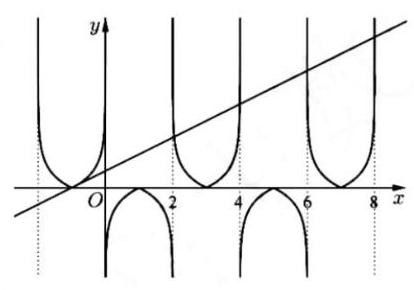
\includegraphics[max width=0.3\textwidth]{images/bo_d5jma53ef24c73bll4ig_81_1035_646_414_290_0.jpg}
\end{center}
\hspace*{3em} 

法一:作出图像如图，观察图像，

当 \(n \rightarrow  \infty\) 时， \({x}_{n + 1} - {x}_{n}\) 趋向于两条渐近线之间的距离，故 \(\mathop{\lim }\limits_{{n \rightarrow  \infty }} \; \left( {{x}_{n + 1} - {x}_{n}}\right)  = 2\)

法二: 当 \(x \in  \lbrack 1,2)\) 时, \(f\left( x\right)  = f\left( {2 - x}\right)  = \ln \left( {2 - x}\right)\) ,

当 \(x \in  ( - 2, - 1\rbrack\) 时, \(f\left( x\right)  =  - f\left( {-x}\right)  =  - \ln \left( {2 + x}\right)\) ,

当 \(x \in  \lbrack  - 1,0)\) 时, \(f\left( x\right)  =  - f\left( {-x}\right)  =  - \ln \left( {-x}\right)\) ,

所以当 \(x \in  ({4n} - 2,{4n} - 1\rbrack\) 时, \(f\left( x\right)  = f\left( {x - {4n}}\right)  =  - \ln \lbrack x - \; \left( {{4n} - 2}\right) \rbrack\) ,

当 \(x \in  \left( {{4n} - 1,{4n}}\right)\) 时, \(f\left( x\right)  = f\left( {x - {4n}}\right)  =  - \ln \left( {{4n} - x}\right)\) ,

不妨令 \(- \ln \left\lbrack  {{x}_{n} - \left( {{4n} - 2}\right) }\right\rbrack   = {x}_{n} + 1, - \ln \left( {{4n} - {x}_{n + 1}}\right)  = {x}_{n + 1} + 1\) ,

所以 \({x}_{n} = {4n} - 2 + \frac{1}{{\mathrm{e}}^{{x}_{n} + 1}},{x}_{n + 1} = {4n} - \frac{1}{{\mathrm{e}}^{{x}_{n + 1} + 1}}\) ,又当 \(n \rightarrow  \infty\) 时, \({x}_{n} \rightarrow  \infty\) ,

所以 \(\mathop{\lim }\limits_{{n \rightarrow  \infty }}\left( {{x}_{n + 1} - {x}_{n}}\right)  = \mathop{\lim }\limits_{{n \rightarrow  \infty }}\left( {2 - \frac{1}{{\mathrm{e}}^{{x}_{n + 1} + 1}} - \frac{1}{{\mathrm{e}}^{{x}_{n} + 1}}}\right)  = 2\) .

【例题】2. (2022 上海春考) 设 \(\left\{  {a}_{n}\right\}\) 为等比数列,设 \({S}_{n}\) 和 \({T}_{n}\) 分别为 \(\left\{  {a}_{n}\right\}\) 的前 \(n\) 项和与前 \(n\) 项积,则下列选项正确的是 ( )

A. 若 \({S}_{2022} \geq  {S}_{2021}\) ,则 \(\left\{  {S}_{n}\right\}\) 为严格递增数列

B. 若 \({T}_{2022} \geq  {T}_{2021}\) ,则 \(\left\{  {T}_{n}\right\}\) 为严格递增数列

C. 若 \(\left\{  {S}_{n}\right\}\) 为严格递增数列,则 \({a}_{2022} > {a}_{2021}\)

D. 若 \(\left\{  {T}_{n}\right\}\) 为严格递增数列,则 \({a}_{2022} > {a}_{2021}\)

【答案】 \(D\)

【解析】 \(A\) . 错误,反例: \(- 1,1, - 1,1,\cdots ;B\) . 错误,反例: \(2, - 2,2, - 2,\cdots\) ;

\(C\) . 错误,反例: \(1,\frac{1}{2},\frac{1}{4},\frac{1}{8},\cdots ;D\) . 正确,下面给出严格证明:

因为 \(\left\{  {T}_{n}\right\}\) 为递增数列,所以 \({a}_{1} > 0,q > 0\) ,否则会出现正负交替,

由 \({T}_{n} > {T}_{n - 1} > 0\) 得 \({a}_{n} > 1,q \geq  1\) ,所以 \({a}_{2022} > {a}_{2021}\) ,故选 \(D\) .

【例题】3. (2021 上海秋考) 已知 \({a}_{i} \in  {N}^{ * }\left( {\mathrm{i} = 1,2,\cdots ,9}\right)\) ,对任意的 \(k \in  {N}^{ * }\left( {2 \leq  k \leq  8}\right) ,{a}_{k} = {a}_{k - 1} + 1\) 或 \({a}_{k} = {a}_{k + 1} - 1\) 中有且仅有一个成立, \({a}_{1} = 6,{a}_{9} = 9\) ,则 \({a}_{1} + \cdots  + {a}_{9}\) 的最小值为\_\_\_\_\_.

【答案】 31

【解析】设 \({b}_{k} = {a}_{k + 1} - {a}_{k}\) ,由题意得 \({b}_{k}\text{ 、 }{b}_{k - 1}\) 恰有一个为 1,

如果 \({b}_{1} = {b}_{3} = {b}_{5} = {b}_{7} = 1\) ,那么 \({a}_{1} = 6,{a}_{2} = 7,{a}_{3} \geq  1,{a}_{4} = {a}_{3} + 1 \geq  2\) ,

同样也有 \({a}_{5} \geq  1,{a}_{6} = {a}_{5} + 1 \geq  2,{a}_{7} \geq  1,{a}_{8} = {a}_{7} + 1 \geq  2\) ,

全部加起来至少是 \(6 + 7 + 1 + 2 + 1 + 2 + 1 + 2 + 9 = {31}\) ;

如果 \({b}_{2} = {b}_{4} = {b}_{6} = {b}_{8} = 1\) ,那么 \({a}_{8} = 8,{a}_{2} \geq  1,{a}_{3} = {a}_{2} + 1 \geq  2\) ,

同样也有 \({a}_{4} \geq  1,{a}_{5} \geq  2,{a}_{6} \geq  1,{a}_{7} \geq  2\) ,

全部加起来至少是 \(6 + 1 + 2 + 1 + 2 + 1 + 2 + 8 + 9 = {32}\) .

综上所述,最小应该是 31 .

【例题】4. (2020 上海春考) 数列 \(\left\{  {a}_{n}\right\}\) 各项均为实数,对任意 \(n \in  {N}^{ * }\) 满足 \({a}_{n + 3} = {a}_{n}\) ,且 \({a}_{n}{a}_{n + 3} - {a}_{n + 1}{a}_{n + 2} \; = c\) 为定值,则下列选项中不可能的是 ( )

A. \({a}_{1} = 1,c = 1\) B. \({a}_{1} = 2,c = 2\) C. \({a}_{1} =  - 1,c = 4\) D. \({a}_{1} = 2,c = 0\)

【答案】 \(B\)

【解析】 \({a}_{n}{a}_{n + 3} - {a}_{n + 1}{a}_{n + 2} = c\) ,因为对任意 \(n \in  {N}^{ * }\) 满足 \({a}_{n + 3} = {a}_{n}\) ,

所以 \(\left\{  \begin{array}{l} {a}_{n}^{2} - {a}_{n + 1}{a}_{n + 2} = c \\  {a}_{n + 1}^{2} - {a}_{n + 2}{a}_{n + 3} = c \end{array}\right.\) ,作差整理得 \({a}_{n + 1} = {a}_{n}\) (常数列, \(c = 0\) ),

或 \({a}_{n} + {a}_{n + 1} + {a}_{n + 2} = 0\) ,

当 \({a}_{n} + {a}_{n + 1} + {a}_{n + 2} = 0\) ,则 \({a}_{n + 1} + {a}_{n + 2} =  - {a}_{n}\) 及 \({a}_{n + 1}{a}_{n + 2} = {a}_{n}^{2} - c\) ,

所以方程 \({x}^{2} + {a}_{n}x + {a}_{n}^{2} - c = 0\) 有两根 \({a}_{n + 1},{a}_{n + 2}\) ,

所以 \(\Delta  = {a}_{n}^{2} - 4\left( {{a}_{n}^{2} - c}\right)  = {4c} - 3{a}_{n}^{2} > 0\) ,所以 \(B\) 错,故选 \(B\) . 2025 版上海高考真题及模拟训练合集

\section*{2. 模拟练习}

【练习】1. (2024 届交附) 若 \(\left\{  {a}_{n}\right\}\) 是以 \({a}_{1}\) 为首项, \(d\) 为公差的等差数列; \(\left\{  {b}_{n}\right\}\) 是以 \({b}_{1}\) 为首项, \(q\) 为公比的等比数列. 则下列说法正确的是\_\_\_\_\_.

 \circled{1} 存在实数 \({a}_{1}\) ，使得不存在实数 \(d \neq  0\) ，满足数列 \(\left\{  {\sin \left( {a}_{n}\right) }\right\}\) 是常数列；

 \circled{2} 存在实数 \(d \neq  0\) ，使得对任意实数 \({a}_{1}\) ，满足数列 \(\left\{  {\sin \left( {a}_{n}\right) }\right\}\) 都是常数列；

 \circled{3} 存在实数 \({b}_{1} \neq  0\) ，使得不存在实数 \(q \neq  1,0\) ，满足数列 \(\left\{  {\sin \left( {b}_{n}\right) }\right\}\) 是常数列；

 \circled{4} 存在实数 \({b}_{1} \neq  0\) ，使得有无穷多个实数 \(q \neq  1,0\) ，满足数列 \(\left\{  {\sin \left( {b}_{n}\right) }\right\}\) 是常数列.

【答案】 \circled{2}  \circled{3}  \circled{4} 

【解析】 \(d = {2\pi }\) ,则对任意 \({a}_{1},\sin \left( {a}_{n}\right)  = \sin \left( {a}_{1}\right)\) 恒成立,故 \circled{1} 错 \circled{2} 对.

取 \({b}_{1} = \pi\) ，任取 \(q \in  Z\) ，则 \({b}_{n} = \pi {q}^{n - 1},\sin \left( {b}_{n}\right)  = 0\) 恒成立，故 \circled{4} 正确.

(更强的命题, \({b}_{1} = \frac{t}{s}\pi\) ,则均存在无数个 \(q \neq  1\) ,使得 \(\sin \left( {b}_{n}\right)\) 为常数,

取 \(q = {2ks} + 1,k \in  Z\) 即可)

只证明 \circled{3} . 取 \({b}_{1} = 1\) ，假设 \(\left\{  {\sin \left( {b}_{n}\right) }\right\}\) 为常数列，

则 \({b}_{n} = {q}^{n - 1} = 1 + {2k\pi }\) 或 \(\pi  - 1 + {2k\pi }\) ,

取 \(n = 2\) ,则 \(q = 1 + 2{k}_{1}\pi\) 或 \(\pi  - 1 + 2{k}_{1}\pi  =  - 1 + \left( {2{k}_{1} - 1}\right) \pi\) ,

\(n = 3\) ,则 \({q}^{2} = 1 + 2{k}_{2}\pi\) 或 \(\pi  - 1 + 2{k}_{2}\pi\) ,

情况一 \(q = 1 + 2{k}_{1}\pi \left( {{k}_{1} \neq  0}\right) ,{q}^{2} = 1 + 2{k}_{2}\pi\) ,则 \({\left( 1 + 2{k}_{1}\pi \right) }^{2} = 1 + 2{k}_{2}\pi\) ,

这是一个关于 \(\pi\) 的一元二次方程,但这是不可能的 \(\left( \pi \right.\) 是超越数 \()\) ,

其他情况同理,所以这样的等比数列不存在.

故正确的是 \circled{2}  \circled{3}  \circled{4} .

【练习】2. (2024 届松二) 若数列 \(\left\{  {a}_{n}\right\}\) 满足条件: 存在正整数 \(k\) ,使得 \({a}_{n + k} + {a}_{n - k} = 2{a}_{n}\) 对一切 \(n \in  {N}^{ * },n \; > k\) 都成立,则称数列 \(\left\{  {a}_{n}\right\}\) 为 \(k\) 级等差数列. 若 \({a}_{n} = {2n} + \sin {\omega n}\left( {\omega \text{ 为常数 }}\right)\) ,且 \(\left\{  {a}_{n}\right\}\) 是 3 级等差数列，则 \(\omega\) 所有可能值的集合为\_\_\_\_\_.

【答案】 \(\omega  \in  \left\{  {\omega \left| {\;\omega  = \frac{2k\pi }{3}}\right. ,k \in  Z}\right\}   \cup  \{ \omega  \mid  \omega  = {k\pi },k \in  Z\}\)

【解析】 \(\left\{  {a}_{n}\right\}\) 是 3 级等差数列,故 \({a}_{n + 3} + {a}_{n - 3} = 2{a}_{n}\) 对一切 \(n \in  {N}^{ * },n > 3\) 都成立.

即 \(2\left( {{2n} + \sin {\omega n}}\right)  = 2\left( {n + 3}\right)  + \sin \left( {{\omega n} + {3\omega }}\right)  + 2\left( {n - 3}\right)  + \sin \left( {{\omega n} - {3\omega }}\right) \left( {n \in  {N}^{ * }}\right)\) ,

所以 \(2\sin {\omega n} = \sin \left( {{\omega n} + {3\omega }}\right)  + \sin \left( {{\omega n} - {3\omega }}\right)  = 2\sin {\omega n}\cos {3\omega }\left( {n \in  {N}^{ * }}\right)\) ,

所以 \(\sin {\omega n} = 0\) 或 \(\cos {3\omega } = 1\) .

当 \(\sin {\omega n} = 0\) 时, \(\omega  = {k\pi }\left( {k \in  Z}\right)\) .

当 \(\cos {3\omega } = 1\) 时, \({3\omega } = {2k\pi }\left( {k \in  Z}\right)\) ,所以 \(\omega  = \frac{2k\pi }{3}\left( {k \in  Z}\right)\) ,

所以 \(\omega  \in  \left\{  {\omega \left| {\;\omega  = \frac{2k\pi }{3}}\right. ,k \in  Z}\right\}   \cup  \{ \omega  \mid  \omega  = {k\pi },k \in  Z\}\) .

【练习】3. 已知数列 \(\left\{  {a}_{n}\right\}\) 是有无穷项的等差数列, \({a}_{1} \geq  0\) ,公差 \(d > 0\) ,若满足条件:  \circled{1}  38 是数列 \(\left\{  {a}_{n}\right\}\) 的项;  \circled{2} 对任意的正整数 \(m,n\left( {m \neq  n}\right)\) ,都存在正整数 \(k\) ,使得 \({a}_{m}{a}_{n} = {a}_{k}\) . 则满足这样的数列的个数是\_\_\_\_\_种.

【答案】69

【解析】设 \(x\) 是数列 \(\left\{  {a}_{n}\right\}\) 中的任意一项,则 \(x + d,x + {2d}\) 均是数列 \(\left\{  {a}_{n}\right\}\) 中的项,

由已知 \({a}_{m}{a}_{n} = {a}_{k}\) ,设 \({a}_{{k}_{1}} = x\left( {x + d}\right) ,{a}_{{k}_{2}} = x\left( {x + {2d}}\right)\) ,

由等差数列定义得 \({a}_{{k}_{2}} - {a}_{{k}_{1}} = {xd} = \left( {{k}_{2} - {k}_{1}}\right)  \cdot  d\) .

因为 \(d \neq  0\) ,所以 \(x = {k}_{2} - {k}_{1} \in  Z\) ,即数列 \(\left\{  {a}_{n}\right\}\) 的每一项均是整数,

所以数列 \(\left\{  {a}_{n}\right\}\) 的每一项均是自然数,且 \(d\) 是正整数.

设 \({a}_{k} = {38}\) ,则 \({a}_{k + 1} = {38} + d\) 是数列 \(\left\{  {a}_{n}\right\}\) 中的项,

所以 \({38} \cdot  \left( {{38} + d}\right)\) 是数列 \(\left\{  {a}_{n}\right\}\) 中的项.

设 \({a}_{m} = {38} \cdot  \left( {{38} + d}\right)\) ,则 \({a}_{m} - {a}_{k} = {38} \cdot  \left( {{38} + d}\right)  - {38} = {38} \times  {37} + {38d} = \left( {m - k}\right)  \cdot  d\) ,

即 \(\left( {m - k - {38}}\right)  \cdot  d = {38} \times  {37}\) .

因为 \(m - k - {38} \in  Z,d \in  {N}^{ * }\) ,故 \(d\) 是 \({38} \times  {37}\) 的约数,

所以 \(d = 1,2,{19},{37},2 \times  {19},2 \times  {37},{19} \times  {37},{38} \times  {37}\) .

当 \(d = 1\) 时， \({a}_{1} = {38} - \left( {k - 1}\right)  \geq  0\) ，得 \(k = 1,2,\cdots ,{38},{39}\) ，

故 \({a}_{1} = {38},{37},\cdots ,2,1,0\) ,共 39 种可能;

当 \(d = 2\) 时, \({a}_{1} = {38} - 2\left( {k - 1}\right)  \geq  0\) ,得 \(k = 1,2,\cdots ,{18},{19},{20}\) ,

故 \({a}_{1} = {38},{36},{34},\cdots ,4,2,0\) ,共 20 种可能;

当 \(d = {19}\) 时, \({a}_{1} = {38} - {19} \times  \left( {k - 1}\right)  \geq  0\) ,得 \(k = 1,2,3\) ,故 \({a}_{1} = {38},{19},0\) ,

共 3 种可能;

当 \(d = {37}\) 时, \({a}_{1} = {38} - {37}\left( {k - 1}\right)  \geq  0\) ,得 \(k = 1,2\) ,故 \({a}_{1} = {38},1\) ,共 2 种可能;

当 \(d = {38}\) 时, \({a}_{1} = {38} - {38} \times  \left( {k - 1}\right)  \geq  0\) ,得 \(k = 1,2\) ,故 \({a}_{1} = {38},0\) ,共 2 种可能;

当 \(d = 2 \times  {37}\) 时, \({a}_{1} = {38} - 2 \times  {37} \times  \left( {k - 1}\right)  \geq  0\) ,得 \(k = 1\) ,故 \({a}_{1} = {38}\) ,

共 1 种可能;

当 \(d = {19} \times  {37}\) 时, \({a}_{1} = {38} - {19} \times  {37} \times  \left( {k - 1}\right)  \geq  0\) ,得 \(k = 1\) ,故 \({a}_{1} = {38}\) ,

共 1 种可能;

当 \(d = {38} \times  {37}\) 时, \({a}_{1} = {38} - {38} \times  {37} \times  \left( {k - 1}\right)  \geq  0\) ,得 \(k = 1\) ,故 \({a}_{1} = {38}\) ,

共 1 种可能.

综上,满足题意的数列 \(\left\{  {a}_{n}\right\}\) 共有 \({39} + {20} + 3 + 2 + 2 + 1 + 1 + 1 = {69}\) (种).

经检验, 这些数列均符合题意, 故满足这样的数列的个数是 69 .

【练习】4. (2025 格致) 已知数列 \(\left\{  {a}_{n}\right\}\) ,若存在数列 \(\left\{  {b}_{n}\right\}\) 满足对任意正整数 \(n\) ,都有

\(\left( {{a}_{n} - {b}_{n}}\right) \left( {{a}_{n + 1} - {b}_{n + 1}}\right)  < 0\) ，则称数列 \(\left\{  {b}_{n}\right\}\) 是 \(\left\{  {a}_{n}\right\}\) 的交错数列. 有下列两个命题: \circled{1} 对任意给定的等差数列 \(\left\{  {a}_{n}\right\}\) ，不存在等差数列 \(\left\{  {b}_{n}\right\}\) ，使得 \(\left\{  {b}_{n}\right\}\) 是 \(\left\{  {a}_{n}\right\}\) 的交错数列;  \circled{2} 对任意给定的等比数列 \(\left\{  {a}_{n}\right\}\) ，都存在等比数列 \(\left\{  {b}_{n}\right\}\) ，使得 \(\left\{  {b}_{n}\right\}\) 是 \(\left\{  {a}_{n}\right\}\) 的交错数列. 下列结论正确的是\_\_\_\_\_ch\_\_\_\_\_:

A.  \circled{1} 与 \circled{2} 都是真命题 B.  \circled{1} 为真命题， \circled{2} 为假命题

C.  \circled{1} 为假命题， \circled{2} 为真命题 D.  \circled{1} 与 \circled{2} 都是假命题

【答案】 \(A\)

【解析】对于 \circled{1} :因为数列 \(\left\{  {a}_{n}\right\}  ,\left\{  {b}_{n}\right\}\) 均为等差数列,

设 \({a}_{n} = {kn} + m,{b}_{n} = {cn} + d\) ,则 \({a}_{n} - {b}_{n} = \left( {k - c}\right) n + m - d\) ,

若 \(k - c > 0\) ,则当 \(n >  - \frac{m - d}{k - c}\) 时, \({a}_{n} - {b}_{n} > 0\) 恒成立,不满足交错数列;

若 \(k - c = 0\) ,则 \({a}_{n} - {b}_{n}\) 的符号不变,不满足交错数列;

若 \(k - c < 0\) ,则当 \(n >  - \frac{m - d}{k - c}\) 时, \({a}_{n} - {b}_{n} < 0\) 恒成立,不满足交错数列;

综上所述，对任意等差数列 \(\left\{  {a}_{n}\right\}\) ， \(\left\{  {b}_{n}\right\}\) ， \(\left\{  {b}_{n}\right\}\) 均不是 \(\left\{  {a}_{n}\right\}\) 的交错数列，故 \circled{1} 正确；

对于 \circled{2} :因为数列 \(\left\{  {a}_{n}\right\}\) 为等比数列，设 \({a}_{n} = a{q}^{n},{aq} \neq  0\) ，

等比数列 \(\left\{  {a}_{n}\right\}\) 的公比为 \(q\) ,

不妨假设 \(a > 0,q > 0,{b}_{n} = a{\left( -2q\right) }^{n}\) ,此时等比数列 \(\left\{  {b}_{n}\right\}\) 的公比为 \(- {2q} < 0\) ,

当 \(n\) 为奇数,则 \({b}_{n} =  - a{q}^{n} \cdot  {2}^{n} < a{q}^{n} = {a}_{n}\) ;

当 \(n\) 为偶数,则 \({b}_{n} = a{q}^{n} \cdot  {2}^{n} > a{q}^{n} = {a}_{n}\) ;

满足 \(\left\{  {b}_{n}\right\}\) 是 \(\left\{  {a}_{n}\right\}\) 的交错数列,

若等比数列 \(\left\{  {a}_{n}\right\}\) 的公比为 \(q < 0\) ，由对称结构，上述结论依然成立，

同理若 \(a < 0\) ，根据对称结构，上述结论依然成立；

综上所述，对任意给定的等比数列 \(\left\{  {a}_{n}\right\}\) ，都存在等比数列 \(\left\{  {b}_{n}\right\}\) ，

使得 \(\left\{  {b}_{n}\right\}\) 是 \(\left\{  {a}_{n}\right\}\) 的交错数列,故 \circled{2} 正确；

故选 \(A\) .

【练习】5. (2024 届华二) 已知数列 \(\left\{  {a}_{n}\right\}\) 不是常数列,前 \(n\) 项和为 \({S}_{n}\) ,且 \({a}_{1} > 0\) . 若对任意正整数 \(n\) ,存在正整数 \(m\) ，使得 \(\left| {{a}_{n} - {S}_{m}}\right|  \leq  {a}_{1}\) ，则称 \(\left\{  {a}_{n}\right\}\) 是“可控数列”. 现给出两个命题: \circled{1} 存在等差数列 \(\left\{  {a}_{n}\right\}\) 是 “可控数列”;  \circled{2} 存在等比数列 \(\left\{  {a}_{n}\right\}\) 是“可控数列”. 则下列判断正确的是 ( ( )

A.  \circled{1} 与 \circled{2} 均为真命题 B.  \circled{1} 与 \circled{2} 均为假命题

C.  \circled{1} 为真命题， \circled{2} 为假命题 D.  \circled{1} 为假命题， \circled{2} 为真命题

【答案】 \(D\)

【解析】对于 \circled{1} ,数列 \(\left\{  {a}_{n}\right\}\) 不是常数列,则 \(d \neq  0\) ,则 \({a}_{n}\) 以一次函数形式变化,

由 \(\left| {{a}_{n} - {S}_{m}}\right|  \leq  {a}_{1}\) 得 \({S}_{m} - {a}_{1} \leq  {a}_{n} \leq  {S}_{m} + {a}_{1},{S}_{m}\) 以二次函数形式变化,

当 \(n\) 充分大时,显然不成立;

对于 \circled{2} ，取 \({a}_{n} = {2}^{n}\) ，则 \({S}_{n} = \frac{2\left( {1 - {2}^{n}}\right) }{1 - 2} = {2}^{n + 1} - 2 = {a}_{n + 1} - {a}_{1}\) ，

当 \(n = 1\) 时，取 \(m = 1\) ，满足 \(\left| {{a}_{n} - {S}_{m}}\right|  \leq  {a}_{1}\) ；

当 \(n \geq  2\) 时,取 \(m = n - 1\) ,满足 \(\left| {{a}_{n} - {S}_{m}}\right|  \leq  {a}_{1}\) ; 故选 \(D\) .

【练习】6. (2025 届大同)已知数列 \(\left\{  {a}_{n}\right\}\) 为无穷数列. 若存在正整数 \(l\) ，使得对任意的正整数 \(n\) ，均有 \({a}_{n + l} \leq  {a}_{n}\) ，则称数列 \(\left\{  {a}_{n}\right\}\) 为“ \(l\) 阶弱减数列”. 有以下两个命题:

 \circled{1} 数列 \(\left\{  {b}_{n}\right\}\) 为无穷数列且 \({b}_{n} = \cos n - \frac{\pi }{8}n\left( {n\text{ 为正整数 }}\right)\) ，则 \(l \geq  5\) 是数列 \(\left\{  {b}_{n}\right\}\) 为“ \(l\) 阶弱减数列”的充分条件;

 \circled{2} 数列 \(\left\{  {c}_{n}\right\}\) 为无穷数列且 \({c}_{n} = \left( {1 - n}\right) \left( {n - 5 + a}\right) \left( {n - 5 - a}\right)  + 1\) ( \(n\) 为正整数)，则存在 \(a \in  \left\lbrack  {0,4}\right\rbrack\) ,使得数列 \(\left\{  {c}_{n}\right\}\) 是 “ \(l\) 阶弱减数列” 的充要条件是 \(l \geq  4\) ; 那么 ( )

A.  \circled{1} 是真命题， \circled{2} 是假命题 B.  \circled{1} 是假命题， \circled{2} 是真命题

C.  \circled{1} 、 \circled{2} 都是真命题 D.  \circled{1} 、 \circled{2} 都是假命题

【答案】 \(A\)

【解析】 \({b}_{n + l} - {b}_{n} = \left\lbrack  {\cos \left( {n + l}\right)  - \frac{\pi }{8}\left( {n + l}\right) }\right\rbrack   - \left( {\cos n - \frac{\pi }{8}n}\right)\)

\(= \cos \left( {n + l}\right)  - \cos n - \frac{l}{8}\pi  =  - 2\sin \left( {n + \frac{l}{2}}\right) \sin \frac{l}{2} - \frac{l}{8}\pi\) ,

数列 \(\left\{  {b}_{n}\right\}\) 为 “ \(l\) 阶弱减数列”,即 \({b}_{n + 1} - {b}_{n} =  - 2\sin \left( {n + \frac{l}{2}}\right) \sin \frac{l}{2} - \frac{l}{8}\pi  \leq  0\) 恒成立,

\(2\sin \frac{l}{2} - \frac{l}{8}\pi  \leq  0,l = 5\) 时, \(2\sin \frac{5}{2} - \frac{5}{8}\pi  \approx   - {1.87625} < 0\) ,

\(l \geq  6\) 时， \(2\sin \frac{l}{2} - \frac{l}{8}\pi  < 2 - \frac{l}{8}\pi  \leq  2 - \frac{6}{8}\pi  \approx   - {0.356} < 0\) ，故 \circled{1} 正确；

\({c}_{n + 1} - {c}_{n} = \left( {1 - n - l}\right) \left( {n + l - 5 + a}\right) \left( {n + l - 5 - a}\right)  - \left( {1 - n}\right) \left( {n - 5 + a}\right) \left( {n - 5 - a}\right)\)

\(= \left( {1 - n - l}\right) \left\lbrack  {{\left( n + l - 5\right) }^{2} - {a}^{2}}\right\rbrack   - \left( {1 - n}\right) \left\lbrack  {{\left( n - 5\right) }^{2} - {a}^{2}}\right\rbrack\)

\(= \left( {1 - n - l}\right) {\left( n + l - 5\right) }^{2} - \left( {1 - n}\right) {\left( n - 5\right) }^{2} + l \cdot  {a}^{2}\) ,

存在 \(a \in  \left\lbrack  {0,4}\right\rbrack\) ,使得数列 \(\left\{  {c}_{n}\right\}\) 是 “ \(l\) 阶弱减数列”,

则 \({\left( {c}_{n + 1} - {c}_{n}\right) }_{\min } = \left( {1 - n - l}\right) {\left( n + l - 5\right) }^{2} - \left( {1 - n}\right) {\left( n - 5\right) }^{2} \leq  0\) ,

即 \(\left( {n - 1}\right) {\left( n - 5\right) }^{2} \leq  \left( {n + l - 1}\right) {\left( n + l - 5\right) }^{2}\) 恒成立,

设 \(f\left( x\right)  = \left( {x - 1}\right) {\left( x - 5\right) }^{2}\) ,则 \(f\left( x\right)  \leq  f\left( {x + l}\right) \left( {x \in  {N}^{ * }}\right)\) 恒成立,

当 \(l = 4\) 时, \(f\left( 2\right)  = 9 > f\left( 6\right)  = 5\) 与 \(f\left( x\right)  \leq  f\left( {x + 4}\right) \left( {x \in  {N}^{ * }}\right)\) 恒成立矛盾,

故 \circled{2} 错误；

故选 \(A\) .

【练习】7. (2025 届交附) \(f\left( x\right)  = \sin {\omega x},\omega  > 0,x \in  \left\lbrack  {-2,2}\right\rbrack  ,y = f\left( x\right)\) 和 \(y = f\left( {f\left( x\right) }\right)\) 的零点按从小到大顺序可以分别构成两个等差数列，则 \(\omega\) 所构成的集合为\_\_\_\_\_

【答案】 \(\left\lbrack  {\frac{\pi }{2},\pi }\right\rbrack   \cup  \left\{  \frac{2\sqrt{3}\pi }{3}\right\}\)

【解析】 \circled{1}  令 \(f\left( x\right)  = 0\) ，则 \({\omega x} = {k\pi }\) ，即 \(x = \frac{k\pi }{\omega }\) ，

因为当 \(k\) 取-1,0,1时， \(x\) 的值为 \(- \frac{\pi }{\omega },0,\frac{\pi }{\omega }\) 满足等差数列，即 \(- 2 \leq   - \frac{\pi }{\omega }\) ，

即 \(\omega  \geq  \frac{\pi }{2}\) 即可

 \circled{2}  令 \(f\left( {f\left( x\right) }\right)  = 0\) ，则 \(f\left( x\right)  = \frac{k\pi }{\omega }\) ， \(k = 0\) 时， \(x = \frac{k\pi }{\omega }\) ，当 \(k =  \pm  1\) 时， \(f\left( x\right)  =  \pm  \frac{\pi }{\omega }\) ，

若 \(x = \frac{\pi }{\omega } > 1\) ,即 \(\omega  < \pi\) 时,则 \(f\left( {f\left( x\right) }\right)  = 0\) 的解与 \(f\left( x\right)  = 0\) 相同,满足题意;

若 \(x = \frac{\pi }{\omega } = 1\) ,即 \(\omega  = \pi\) 时,令 \(\sin {\omega x} =  \pm  1\) ,即 \({\pi x} = \frac{\pi }{2} + {k\pi }\) ,则 \(x = \frac{1 + {2k}}{2}\) ,

则 \(f\left( {f\left( x\right) }\right)  = 0\) 的解 \(- 2,\frac{-3}{2}, - 1, - \frac{1}{2},0,\frac{1}{2},1,\frac{3}{2},2\) ,满足等差数列;

若 \(x = \frac{\pi }{\omega } < 1\) ,即 \(\omega  > \pi\) 时,

因为 \(k = 0\) 时 \(f\left( {f\left( x\right) }\right)  = 0\) 已存在至少三个解 \(- \frac{\pi }{\omega },0,\frac{\pi }{\omega }\) ,

由三角函数图像得 \(f\left( x\right)  = \frac{\pi }{\omega }\) 在 \(\left( {0,\frac{\pi }{\omega }}\right)\) 存在两个解,即 \(0,{x}_{1},{x}_{2},\frac{\pi }{\omega }\) 成等差数列,

即 \({x}_{1} = \frac{\pi }{3\omega }\) ,则 \(\sin \frac{\pi }{3} = \frac{\sqrt{3}}{2} = \frac{\pi }{\omega }\) ,即 \(\omega  = \frac{2\sqrt{3}\pi }{3}\) ,

综上所述， \(\omega\) 所构成的集合为 \(\left\lbrack  {\frac{\pi }{2},\pi }\right\rbrack   \cup  \left\{  \frac{2\sqrt{3}\pi }{3}\right\}\)

【练习】8. 已知 \(\left\{  {a}_{n}\right\}\) 为非常数数列且 \({a}_{n} \neq  0,{a}_{1} = \mu ,{a}_{n + 1} = {a}_{n} + \sin \left( {2{a}_{n}}\right)  + \lambda \left( {\mu ,\lambda  \in  R,n \in  {N}^{ * }}\right)\) ,则下列说法错误的是 ( )

A. 对任意的 \(\lambda ,\mu\) ，数列 \(\left\{  {a}_{n}\right\}\) 为单调递增数列

B. 对任意的正数 \(\varepsilon\) ，存在 \(\lambda ,\mu ,{n}_{0}\left( {{n}_{0} \in  {N}^{ * }}\right)\) ，当 \(n > {n}_{0}\) 时， \(\left| {{a}_{n} - 1}\right|  < \varepsilon\)

C. 不存在 \(\lambda ,\mu\) ,使得数列 \(\left\{  {a}_{n}\right\}\) 的周期为 2

D. 不存在 \(\lambda ,\mu\) ,使得 \(\left| {{a}_{n} + {a}_{n + 2} - 2{a}_{n - 1}}\right|  > 2\)

【答案】 \(A\)

【解析】当 \(\lambda  <  - 1\) 时,可知 \(\left\{  {a}_{n}\right\}\) 为单调递减数列,知 \(A\) 错误; 令 \(\lambda  =  - \sin 2,f\left( x\right)  = x + \sin {2x} - \sin 2\) , \(g\left( x\right)  = x\) ,利用导数可求得 \(f\left( x\right)\) 在 \(\left\lbrack  {0,1}\right\rbrack\) 上单调递增,令 \(f\left( x\right)  = g\left( x\right) \left( {0 \leq  x \leq  1}\right)\) ,可解得 \(x = \frac{\pi }{2}\)

-1 或 \(x = 1\) ，结合图象可确定 \(B\) 正确；采用反证法，若周期为 2，可化简得到 \(2{a}_{n} + \sin \left( {2{a}_{n}}\right)  = \; 2{a}_{n + 1} + \sin \left( {2{a}_{n + 1}}\right)\) ,令 \(h\left( x\right)  = x + \sin x\) ,利用导数可求得 \(h\left( x\right)\) 单调递增,由此确定 \({a}_{n + 1} = {a}_{n}\) ,与已知矛盾,知 \(C\) 正确; 利用已知等式化简得到 \(\left| {{a}_{n} + {a}_{n + 2} - 2{a}_{n - 1}}\right|  = \left| {\sin \left( {2{a}_{n + 1}}\right)  - \sin \left( {2{a}_{n}}\right) }\right|  \leq  2\) ,知 \(D\) 正确.

对于 \(A\) ,当 \(\lambda  <  - 1\) 时, \({a}_{n + 1} - {a}_{n} = \sin \left( {2{a}_{n}}\right)  + \lambda  < 0\) ,此时 \(\left\{  {a}_{n}\right\}\) 为单调递减数列, \(A\) 错误;

对于 \(B\) ,令 \(\lambda  =  - \sin 2\) ,令 \(f\left( x\right)  = x + \sin {2x} - \sin 2,g\left( x\right)  = x\) ,则 \(f\left( 1\right)  = g\left( 1\right)  = 1\) ;

\(\because {f}^{\prime }\left( x\right)  = 1 + 2\cos {2x}\) ,令 \({f}^{\prime }\left( x\right)  = 0\) ,则 \(\cos {2x} =  - \frac{1}{2}\) ,可取 \(x = \frac{\pi }{3}\) ,

\(\therefore\) 当 \(x \in  \left\lbrack  {0,1}\right\rbrack\) 时, \({f}^{\prime }\left( x\right)  > 0,\therefore f\left( x\right)\) 在 \(\left\lbrack  {0,1}\right\rbrack\) 上单调递增;

令 \(f\left( x\right)  = g\left( x\right) \left( {0 \leq  x \leq  1}\right)\) ,解得: \(x = \frac{\pi }{2} - 1\) 或 \(x = 1\) ,

\begin{center}
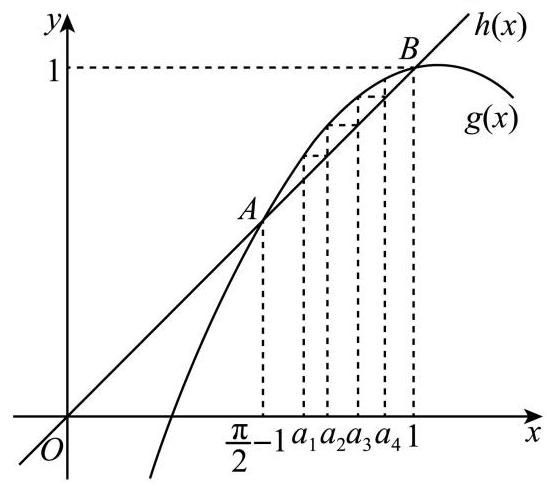
\includegraphics[max width=0.4\textwidth]{images/bo_d5jma53ef24c73bll4ig_87_291_685_547_486_0.jpg}
\end{center}
\hspace*{3em} 

如图所示，在区间 \(\left( {\frac{\pi }{2} - 1,1}\right)\) 内，总能找到一个 \({a}_{1}\) ，使得 \({a}_{n}\) 的极限为1， \(B\) 正确；

对于 \(C\) ，假设存在 \(\lambda ,\mu\) ，使得数列 \(\left\{  {a}_{n}\right\}\) 的周期为 2，则 \({a}_{n + 2} = {a}_{n}\) ；

\(\therefore \left\{  {\begin{array}{l} {a}_{n + 1} = {a}_{n} + \sin \left( {2{a}_{n}}\right)  + \lambda \\  {a}_{n + 2} = {a}_{n + 1} + \sin \left( {2{a}_{n + 1}}\right)  + \lambda  \end{array},\therefore {a}_{n + 2} - {a}_{n + 1} = {a}_{n + 1} - {a}_{n} + \sin \left( {2{a}_{n + 1}}\right)  - \sin \left( {2{a}_{n}}\right) ,}\right.\)

\(\therefore {a}_{n} - {a}_{n + 1} = {a}_{n + 1} - {a}_{n} + \sin \left( {2{a}_{n + 1}}\right)  - \sin \left( {2{a}_{n}}\right)\) ,即 \(2{a}_{n} + \sin \left( {2{a}_{n}}\right)  = 2{a}_{n + 1} + \sin \left( {2{a}_{n + 1}}\right)\) ;

令 \(h\left( x\right)  = x + \sin x\) ,则 \({h}^{\prime }\left( x\right)  = 1 + \cos x \geq  0,\therefore h\left( x\right)\) 在 \(R\) 上单调递增,

则由 \(h\left( {2{a}_{n}}\right)  = h\left( {2{a}_{n + 1}}\right)\) 得: \({a}_{n} = {a}_{n + 1}\) ,即 \(\left\{  {a}_{n}\right\}\) 为常数列,与已知矛盾,

\(\therefore\) 假设错误,即不存在 \(\lambda ,\mu\) ,使得数列 \(\left\{  {a}_{n}\right\}\) 的周期为 \(2,C\) 正确;

对于 \(D,\because \left\{  \begin{array}{l} {a}_{n + 1} = {a}_{n} + \sin \left( {2{a}_{n}}\right)  + \lambda \\  {a}_{n + 2} = {a}_{n + 1} + \sin \left( {2{a}_{n + 1}}\right)  + \lambda  \end{array}\right.\) ,

\(\therefore \left| {{a}_{n} + {a}_{n + 2} - 2{a}_{n - 1}}\right|  = \left| {\left( {{a}_{n + 2} - {a}_{n + 1}}\right)  - \left( {{a}_{n + 1} - {a}_{n}}\right) }\right|  = \left| {\sin \left( {2{a}_{n + 1}}\right)  - \sin \left( {2{a}_{n}}\right) }\right|  \leq  2\) ,

\(\therefore\) 不存在 \(\lambda ,\mu\) ,使得 \(\left| {{a}_{n} + {a}_{n + 2} - 2{a}_{n - 1}}\right|  > 2,D\) 正确.

故选: \(A\) .

【练习】9. (2024 届华二) 已知无穷实数列 \(\left\{  {a}_{n}\right\}\) 的前 \(n\) 项和为 \({S}_{n}\) . 若数列 \(\left\{  {S}_{n}\right\}\) 既有最大项,也有最小项,有下列两个命题:  \circled{1} 存在 \(\left\{  {a}_{n}\right\}\) ,使得 \({a}_{1} > 0\) 且数列 \(\left\{  \left| {a}_{n}\right| \right\}\) 严格减 \circled{2} 存在 \(\left\{  {a}_{n}\right\}\) ,使得 \({a}_{1} < 0\) 且数列 \(\left\{  \left| {a}_{n}\right| \right\}\) 严格增. 则 ( )

A.  \circled{1} 真命题 \circled{2} 假命题 B.  \circled{1} 假命题 \circled{2} 真命题

C.  \circled{1} 真命题 \circled{2} 真命题 D.  \circled{1} 真命题 \circled{2} 假命题

【答案】 \(C\)

【解析】对 \circled{1} ，我们把他看成 5 个人分 1 个球的问题，先问每个人要1 个小球，因此总共有 6 个小球，分给 5 个人需要插 4 块板，6 个小球有 5 个缝隙可以插板，有 \({C}_{5}^{4} = 5\) 种

取 \({a}_{n} = {\left( -\frac{1}{2}\right) }^{n - 1}\) 即可.

对 \circled{2} ，我们可以构造一个前几项就让数列的和取到了最大值和最小值，而后续是摆动的，对数列的最值影响非常小的数列，比如取 \({a}_{1} =  - 1,{a}_{2} =  - 2,{a}_{3} =  - 3,{a}_{4} =  - {3.1},{a}_{5} = {3.11}\) ，

当 \(n \geq  6\) 时, \({a}_{n} = {\left( -1\right) }^{n}{3.11}\cdots 1\left( {n - 3\text{ 个 1 }}\right)\) ,这样后续每相邻两个 \({a}_{n}\) 对 \({Sn}\) 的影响只有约等于 \(\pm  3\) ,则 \({S}_{n}\) 的最大、最小值分别为 \({S}_{1} =  - 1,{S}_{4} =  - {9.1}\) .

故选 \(C\) .

【练习】10. (2025 届复附) 设 \(\left\{  {a}_{n}\right\}\) 是由正整数组成且项数为 \(m\) 的数列,满足当 \(1 \leq  t \leq  m - 1\) ,都有 \({a}_{i} \leq \; {a}_{t + 1}\) . 已知 \({a}_{1} = 1,{a}_{m} = {100}\) ,数列 \(\left\{  {a}_{n}\right\}\) 任意相邻两项的差的绝对值不超过 1,若对于 \(\left\{  {a}_{n}\right\}\) 中任意序数不同的两项 \({a}_{s}\) 和 \({a}_{t}\) ，在剩下的项中总存在序数不同的两项 \({a}_{p}\) 和 \({a}_{q}\) ，使得 \({a}_{s} + {a}_{t} = {a}_{p} + \; {a}_{q}\) ,则 \(\mathop{\sum }\limits_{{i = 1}}^{m}{a}_{i}\) 的最小值为\_\_\_\_\_.

【答案】5454

【解析】法一: 因为数列 \(\left\{  {a}_{n}\right\}\) 任意相邻两项的差的绝对值不超过 \(1,{a}_{1} = 1\) ,

所以 \(0 \leq  {a}_{2} \leq  2\) ,

又 \(\left\{  {a}_{n}\right\}\) 是由正整数组成且项数为 \(m\) 的增数列,所以 \({a}_{2} = 1\) 或 \({a}_{2} = 2\) ,

当 \({a}_{2} = 2\) 时， \({a}_{4} \geq  {a}_{3} \geq  2\) ，此时 \({a}_{1} + {a}_{2} = 3 < {a}_{3} + {a}_{4}\) ，

与在剩下的项中总存在序数不同的两项 \({a}_{p}\) 和 \({a}_{q}\) ,使得 \({a}_{s} + {a}_{t} = {a}_{p} + {a}_{q}\) 矛盾,

所以 \({a}_{2} = 1\) ,类似地,必有 \({a}_{3} = 1,{a}_{4} = 1,{a}_{5} = 2,{a}_{6} = 2\) ,

由 \({a}_{s} + {a}_{t} = {a}_{p} + {a}_{q}\) 得前 6 项任意两项之和小于等于 3 时,均符合,

\(\mathop{\sum }\limits_{{i = 1}}^{m}{a}_{i} = {a}_{1} + {a}_{2} + \cdots  + {a}_{m}\) 要最小,则每一项尽可能小,

则 \({a}_{5} + {a}_{6} = 4 = {a}_{1} + {a}_{7} \Rightarrow  {a}_{7} = 3\) ,

同理, \({a}_{8} = 4,{a}_{9} = 5,\cdots ,{a}_{m - 6} = {98}\) ,

由对称性得最后 6 项为 \({a}_{m} = {a}_{m - 1} = {a}_{m - 2} = {a}_{m - 3} = {100},{a}_{m - 4} = {a}_{m - 5} = {99}\) ,

则 \(\mathop{\sum }\limits_{{i = 1}}^{m}{a}_{i} = {a}_{1} + {a}_{2} + \cdots  + {a}_{m}\) 的最小值 \(= \frac{\left( {1 + {99}}\right)  \cdot  {99}}{2} + 4 \times  {100} + 3 \times  1 + 2 + {99}\)

\(= {5454}\) .

法二: 令 \(s = 1,t = 2 \Rightarrow  {a}_{s} + {a}_{t} = 1 + {a}_{t} = {a}_{p} + {a}_{q}\) ,

因为数列 \(\left\{  {a}_{n}\right\}\) 递增,所以,至少要有 4 个 1 ,

即 \({a}_{1} = {a}_{2} = {a}_{3} = {a}_{4} = 1\) ,同理,令 \(s = m - 1,t = m \Rightarrow  {a}_{s} + {a}_{t} = {a}_{m - 1} + {100} = {a}_{p} + {a}_{q}\) ,

因为数列 \(\left\{  {a}_{n}\right\}\) 递增,至少需要 4 个 100 ,

继续枚举计算,得 \({a}_{5} = {a}_{6} = 2,{a}_{7} = 3,{a}_{8} = 4,\cdots\) ,

\({a}_{m - 6} = {98},{a}_{m - 5} = {a}_{m - 4} = {99},{a}_{m - 3} = {a}_{m - 2} = {a}_{m - 1} = {a}_{m} = {100}\) ,

故此数列,可安排为 \(1,1,1,1,2,2,3,4,5,\cdots ,{97},{98},{99},{99},{100},{100},{100},{100}\) ,

则 \(\mathop{\sum }\limits_{i}^{m}{a}_{i} = 4 + {400} + {101} + \frac{\left( {2 + {99}}\right)  \times  {98}}{2} = {5454}\) .

\section*{板块三: 基础主观题}

\section*{1. 真题回顾}

【例题】1. (2022 上海春考) 设有无穷数列 \(\left\{  {a}_{n}\right\}\) ,记 \(\left\{  {a}_{n}\right\}\) 的前 \(n\) 项和为 \({S}_{n}\) ,其中 \({a}_{2} = 1\) .

(1)若 \(\left\{  {a}_{n}\right\}\) 为等比数列,且 \({S}_{2} = 3\) ，求该数列所有项的和；

(2)若 \(\left\{  {a}_{n}\right\}\) 为等差数列，对任意 \(n \in  {N}^{ * }\) 均满足 \({S}_{2n} \geq  n\) ，求公差 \(d\) 的取值范围.

【解析】(1) 设公比为 \(q,{a}_{1} = {S}_{2} - {a}_{2} = 2\) ,所以 \(q = \frac{{a}_{2}}{{a}_{1}} = \frac{1}{2}\) ,

故该数列所有项的和为 \(\frac{{a}_{1}}{1 - q} = 4\) ;

(2) \({a}_{1} = 1 - d,{S}_{2n} = {2n}{a}_{1} + \frac{{2n}\left( {{2n} - 1}\right) }{2}d = {2d}{n}^{2} + \left( {2 - {3d}}\right) n \geq  n\) 恒成立,

即 \(\left( {3 - {2n}}\right) d \leq  1\) 恒成立,

法一: 当 \(n = 1\) 时, \(d \leq  1\) ; 当 \(n \geq  2\) 时, \(d \geq  \frac{1}{3 - {2n}}\) 恒成立,

因为 \(\frac{1}{3 - {2n}} \in  \lbrack  - 1,0)\) ,所以 \(d \geq  0\) ,

所以公差 \(d\) 的取值范围是 \(\left\lbrack  {0,1}\right\rbrack\) .

法二: 令 \(f\left( n\right)  = \left( {3 - {2n}}\right) d =  - {2dn} + {3d}\) ,则 \(f\left( n\right)  \leq  1\) 恒成立,

所以 \(\left\{  \begin{array}{l}  - {2d} \leq  0 \\  f\left( 1\right)  = d \leq  1 \end{array}\right.\) ,所以公差 \(d\) 的取值范围是 \(\left\lbrack  {0,1}\right\rbrack\) .

【例题】2. (2021 上海秋考) 已知一企业今年第一季度的营业额为 1.1 亿元, 往后每个季度增加 0.05 亿元,第一季度的利润为 0.16 亿元,往后每一季度比前一季度增长 4\%.

(1)求今年起的前 20 个季度的总营业额;

(2)请问哪一季度的利润首次超过该季度营业额的 18\%？

【解析】(1) 由题意得可将每个季度的营业额看作等差数列,

则首项 \({a}_{1} = {1.1}\) ，公差 \(d = {0.05}\) ，

所以 \({S}_{20} = {20}{a}_{1} + \frac{{20}\left( {{20} - 1}\right) }{2}d = {20} \times  {1.1} + {10} \times  {19} \times  {0.05} = {31.5}\) ,

即营业额前 20 季度的和为 31.5 亿元.

(2)法一:假设今年第一季度往后的第 \(n\left( {n \in  {N}^{ * }}\right)\) 季度的利润首次超过该季度营业

额的 18\%,则 \({0.16} \times  {\left( 1 + 4\% \right) }^{n} > \left( {{1.1} + {0.05n}}\right)  \cdot  {18}\%\) ,

令 \(f\left( n\right)  = {0.16} \times  {\left( 1 + 4\% \right) }^{n} - \left( {{1.1} + {0.05n}}\right)  \cdot  {18}\% \left( {n \in  {N}^{ * }}\right)\) ,

即要解 \(f\left( n\right)  > 0\) ,当 \(n \geq  2\) 时, \(f\left( n\right)  - f\left( {n - 1}\right)  = {0.0064} \cdot  {\left( 1 + 4\% \right) }^{n - 1} - {0.009}\) ,

令 \(f\left( n\right)  - f\left( {n - 1}\right)  > 0\) ,解得 \(n \geq  {10}\) ,

即当 \(1 \leq  n \leq  9\) 时, \(f\left( n\right)\) 递减; 当 \(n \geq  {10}\) 时, \(f\left( n\right)\) 递增,

由于 \(f\left( 1\right)  < 0\) ，因此 \(f\left( n\right)  > 0\) 的解只能在 \(n \geq  {10}\) 时取得，

经检验, \(f\left( {24}\right)  < 0,f\left( {25}\right)  > 0\) ,

所以今年第一季度往后的第 25 个季度的利润首次超过该季度营业额的 18\%.

法二: 设今年第一季度往后的第 \(n\left( {n \in  {N}^{ * }}\right)\) 季度的利润与该季度营业额的比为

\({a}_{n}\) ,则 \(\frac{{a}_{n + 1}}{{a}_{n}} = \frac{{1.04}\left( {{1.05} + {0.05n}}\right) }{{1.1} + {0.05n}} = {1.04} - \frac{1.04}{{22} + n} = 1 + {0.04}\left( {1 - \frac{26}{{22} + n}}\right)\) ,

所以数列 \(\left\{  {a}_{n}\right\}\) 满足 \({a}_{1} > {a}_{2} > {a}_{3} > {a}_{4} = {a}_{5} < {a}_{6} < {a}_{7} < \cdots\) ,

注意到, \({a}_{25} = {0.178},{a}_{26} = {0.181}\) ,

2025 版上海高考真题及模拟训练合集

所以今年第一季度往后的第 25 个季度利润首次超过该季度营业额的 18\%.

【例题】3. (2020 上海春考) 已知各项均为正数的数列 \(\left\{  {a}_{n}\right\}\) ,其前 \(n\) 项和为 \({S}_{n},{a}_{1} = 1\) .

(1)若数列 \(\left\{  {a}_{n}\right\}\) 为等差数列， \({S}_{10} = {70}\) ，求数列 \(\left\{  {a}_{n}\right\}\) 的通项公式；

(2)若数列 \(\left\{  {a}_{n}\right\}\) 为等比数列， \({a}_{4} = \frac{1}{8}\) ，求满足 \({S}_{n} > {{100}{a}_{n}}\) 时 \(n\) 的最小值.

【解析】(1) 数列 \(\left\{  {a}_{n}\right\}\) 为公差为 \(d\) 的等差数列, \({S}_{10} = {70},{a}_{1} = 1\) ,

得 \({10} + \frac{1}{2} \times  {10} \times  {9d} = {70}\) ,解得 \(d = \frac{4}{3}\) ,则 \({a}_{n} = 1 + \frac{4}{3}\left( {n - 1}\right)  = \frac{4}{3}n - \frac{1}{3}\) ;

(2)数列 \(\left\{  {a}_{n}\right\}\) 为公比为 \(q\) 的等比数列， \({a}_{4} = \frac{1}{8}\) ， \({a}_{1} = 1\) ，

得 \({q}^{3} = \frac{1}{8}\) ,即 \(q = \frac{1}{2}\) ,则 \({a}_{n} = {\left( \frac{1}{2}\right) }^{n - 1},{S}_{n} = \frac{1 - {\left( \frac{1}{2}\right) }^{n}}{1 - \frac{1}{2}} = 2 - {\left( \frac{1}{2}\right) }^{n - 1}\) ,

\({S}_{n} > {100}{a}_{n}\) ,即 \(2 - {\left( \frac{1}{2}\right) }^{n - 1} > {100} \cdot  {\left( \frac{1}{2}\right) }^{n - 1}\) ,

即 \({2}^{n} > {101}\) ,得 \(n \geq  7\) ,即 \(n\) 的最小值为 7 .

【例题】4. (2019 上海春考) 已知数列 \(\left\{  {a}_{n}\right\}  ,{a}_{1} = 3\) ,前 \(n\) 项和为 \({S}_{n}\) .

(1)若 \(\left\{  {a}_{n}\right\}\) 为等差数列,且 \({a}_{4} = {15}\) ，求 \({S}_{n}\) ；

(2)若 \(\left\{  {a}_{n}\right\}\) 为等比数列,且 \(\mathop{\lim }\limits_{{n \rightarrow  \infty }}{S}_{n} < {12}\) ,求公比 \(q\) 的取值范围.

【解析】(1) 因为 \({a}_{4} = {a}_{1} + {3d} = 3 + {3d} = {15}\) ,所以 \(d = 4\) ,

所以 \({S}_{n} = {3n} + \frac{n\left( {n - 1}\right) }{2} \times  4 = 2{n}^{2} + n\) ;

(2) 因为 \(\mathop{\lim }\limits_{{n \rightarrow  \infty }}{S}_{n}\) 存在,所以 \(- 1 < q < 1,q \neq  0\) ,所以 \(\mathop{\lim }\limits_{{n \rightarrow  \infty }}{S}_{n} = \mathop{\lim }\limits_{{n \rightarrow  \infty }}\frac{3\left( {1 - {q}^{n}}\right) }{1 - q} = \frac{3}{1 - q}\) ,

所以 \(\frac{3}{1 - q} < {12}\) ,所以 \(q < \frac{3}{4}\) ,所以 \(- 1 < q < 0\) 或 \(0 < q < \frac{3}{4}\) ,

所以公比 \(q\) 的取值范围为 \(\left( {-1,0}\right)  \cup  \left( {0,\frac{3}{4}}\right)\) .

【例题】5. (2016 上海春考) 已知数列 \(\left\{  {a}_{n}\right\}\) 是公差为 2 的等差数列.

(1) \({a}_{1},{a}_{3},{a}_{4}\) 成等比数列,求 \({a}_{1}\) 的值;

(2) 设 \({a}_{1} =  - {19}\) ，数列 \(\left\{  {a}_{n}\right\}\) 的前 \(n\) 项和为 \({S}_{n}\) . 数列 \(\left\{  {b}_{n}\right\}\) 满足 \({b}_{1} = 1,{b}_{n + 1} - {b}_{n} = {\left( \frac{1}{2}\right) }^{n}\) ，记 \({c}_{n} = {S}_{n} \; + {2}^{n - 1} \cdot  {b}_{n}\left( {n \in  {N}^{ * }}\right)\) ,求数列 \(\left\{  {c}_{n}\right\}\) 的最小项 \({c}_{{n}_{0}}\) (即 \({c}_{{n}_{0}} \leq  {c}_{n}\) 对任意 \(n \in  {N}^{ * }\) 成立).

【解析】(1) 因为数列 \(\left\{  {a}_{n}\right\}\) 是公差为 2 的等差数列, \({a}_{1},{a}_{3},{a}_{4}\) 等比数列,

所以 \({\left( {a}_{1} + 2d\right) }^{2} = {a}_{1}\left( {{a}_{1} + {3d}}\right)\) ,解得 \(d = 2,{a}_{1} =  - 8\) ,

(2) \({b}_{n} = {b}_{1} + \left( {{b}_{2} - {b}_{1}}\right)  + \left( {{b}_{3} - {b}_{2}}\right)  + \cdots  + \left( {{b}_{n} - {b}_{n - 1}}\right)\)

\(= 1 + \frac{1}{2} + {\left( \frac{1}{2}\right) }^{2} + \cdots  + {\left( \frac{1}{2}\right) }^{n - 1}\)

\(= \frac{1 - {\left( \frac{1}{2}\right) }^{n}}{1 - \frac{1}{2}} = 2 - {\left( \frac{1}{2}\right) }^{n - 1}\) .

\({S}_{n} =  - {19n} + \frac{n\left( {n - 1}\right) }{2} \cdot  2 = {n}^{2} - {20n},\)

\({c}_{n} = {S}_{n} + {2}^{n - 1} \cdot  {b}_{n} = {n}^{2} - {20n} + {2}^{n - 1} \cdot  \left( {2 - {\left( \frac{1}{2}\right) }^{n - 1}}\right)  = {n}^{2} - {20n} + {2}^{n} - 1,\)

\({c}_{n + 1} - {c}_{n} = {\left( n + 1\right) }^{2} - {20}\left( {n + 1}\right)  + {2}^{n + 1} - 1 - \left( {{n}^{2} - {20n} + {2}^{n} - 1}\right)  = {2n} - {19} + {2}^{n}\) ,

由题意得 \(n \geq  5\) ,上式大于零,即 \({c}_{5} < {c}_{6} < \cdots  < {c}_{n}\) ,

进一步, \({2n} + {2}^{n}\) 是关于 \(n\) 的增函数,

因为 \(2 \times  4 + {2}^{4} = {24} > {19},2 \times  3 + {2}^{3} = {14} < {19}\) ,

所以 \({c}_{1} > {c}_{2} > {c}_{3} > {c}_{4} < {c}_{5} < \cdots  < {c}_{9} < {c}_{10} < \cdots  < {c}_{n}\) ,

所以 \({\left( c\right) }_{\min } = {c}_{{n}_{0}} = {c}_{4} =  - {49}\) .

【例题】6. (2013 上海春考) 在平面直角坐标系 \({xOy}\) 中,点 \(A\) 在 \(y\) 轴正半轴上,点 \({P}_{n}\) 在 \(x\) 轴上,其横坐标

\begin{center}
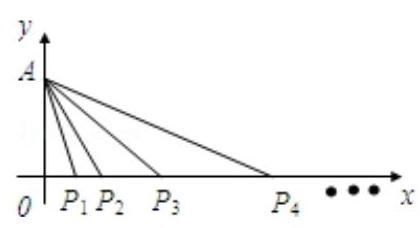
\includegraphics[max width=0.3\textwidth]{images/bo_d5jma53ef24c73bll4ig_91_1037_524_420_228_0.jpg}
\end{center}
\hspace*{3em} 

为 \({x}_{n}\) ,且 \(\left\{  {x}_{n}\right\}\) 是首项为 1、公比为 2 的等比数列,记 \(\angle {P}_{n}A{P}_{n + 1} \; = {\theta }_{n},n \in  {N}^{ * }\) .

(1)若 \({\theta }_{3} = \arctan \frac{1}{3}\) ，求点 \(A\) 的坐标；

(2)若点 \(A\) 的坐标为 \(\left( {0,{8\sqrt{2}}}\right)\) ，求 \({\theta }_{n}\) 的最大值及相应 \(n\) 的值.

【解析】(1) 设 \(A\left( {0,t}\right)\) ,由题意得 \({x}_{n} = {2}^{n - 1}\) .

由 \({\theta }_{3} = \arctan \frac{1}{3}\) 得 \(\tan {\theta }_{3} = \frac{1}{3}\) ,

而 \(\tan {\theta }_{3} = \tan \left( {\angle {OA}{P}_{4} - \angle {OA}{P}_{3}}\right)  = \frac{\frac{{x}_{4}}{t} - \frac{{x}_{3}}{t}}{1 + \frac{{x}_{4}}{t} \cdot  \frac{{x}_{3}}{t}} = \frac{4t}{{t}^{2} + {32}}\) ,

所以 \(\frac{4t}{{t}^{2} + {32}} = \frac{1}{3}\) ,解得 \(t = 4\) 或 \(t = 8\) .

故点 \(A\) 的坐标为 \(\left( {0,4}\right)\) 或 \(\left( {0,8}\right)\) .

(2)由题意得点 \({P}_{n}\) 的坐标为 \(\left( {{2}^{n - 1},0}\right)\) ， \(\tan \angle {OA}{P}_{n} = \frac{{2}^{n - 1}}{8\sqrt{2}}\) .

所以 \(\tan {\theta }_{n} = \tan \left( {\angle {OA}{P}_{n + 1} - \angle {OA}{P}_{n}}\right)  = \frac{\frac{{2}^{n}}{8\sqrt{2}} - \frac{{2}^{n - 1}}{8\sqrt{2}}}{1 + \frac{{2}^{n}}{8\sqrt{2}} \cdot  \frac{{2}^{n - 1}}{8\sqrt{2}}} = \frac{1}{\frac{{16}\sqrt{2}}{{2}^{n}} + \frac{{2}^{n}}{8\sqrt{2}}}\) .

因为 \(\frac{{16}\sqrt{2}}{{2}^{n}} + \frac{{2}^{n}}{8\sqrt{2}} \geq  2\sqrt{2}\) ,所以 \(\tan {\theta }_{n} \leq  \frac{1}{2\sqrt{2}} = \frac{\sqrt{2}}{4}\) ,

当且仅当 \(\frac{{16}\sqrt{2}}{{2}^{n}} = \frac{{2}^{n}}{8\sqrt{2}}\) ,即 \(n = 4\) 时取等号.

因为 \(0 < {\theta }_{n} < \frac{\pi }{2},y = \tan x\) 在 \(\left( {0,\frac{\pi }{2}}\right)\) 上为增函数,

所以当 \(n = 4\) 时， \({\theta }_{n}\) 最大，其最大值为 \(\arctan \frac{\sqrt{2}}{4}\) .

\section*{2. 模拟练习}

【练习】1. (23 届虹口二模) 记 \({S}_{n}\) 为数列 \(\left\{  {a}_{n}\right\}\) 的前 \(n\) 项和,已知 \({a}_{1} = 2,{a}_{n + 1} = {S}_{n}\) ( \(n\) 为正整数).

(1)求数列 \(\left\{  {a}_{n}\right\}\) 的通项公式;

(2)设 \({b}_{n} = {\log }_{2}{a}_{n}\) ，若 \({b}_{m} + {b}_{m + 1} + {b}_{m + 2} + \cdots  + {b}_{m + 9} = {145}\) ，求正整数 \(m\) 的值.

【解析】(1) 由 \({a}_{1} = 2,{a}_{n + 1} = {S}_{n}\) ,得 \({a}_{2} = {S}_{1} = {a}_{1} = 2\) ,

且当 \(n \geq  2\) 时 \({a}_{n} = {S}_{n} - {S}_{n - 1} = {a}_{n + 1} - {a}_{n}\) ,即 \(\frac{{a}_{n + 1}}{{a}_{n}} = 2\left( {n \geq  2}\right)\) . 3 分

所以，数列 \(\left\{  {a}_{n}\right\}\) 从第 2 项开始构成以 \({a}_{2} = 2\) 为首项，2 为公比的等比数列，

故数列 \(\left\{  {a}_{n}\right\}\) 的通项公式为: \({a}_{n} = \left\{  \begin{array}{ll} 2, & n = 1 \\  {2}^{n - 1}, & n \geq  2 \end{array}\right.\) ； 6 分

(2)当 \(n \geq  2\) 时， \({b}_{n} = {\log }_{2}{a}_{n} = {\log }_{2}{2}^{n - 1} = n - 1\) ，

又 \({b}_{1} = {\log }_{2}{a}_{1} = {\log }_{2}2 = 1\) . 8 分

当 \(m = 1\) 时, \({b}_{1} + {b}_{2} + {b}_{3} + \cdots  + {b}_{10} = 1 + \left( {1 + 2 + \cdots  + 9}\right)  = {46}\) ,

不满足条件; 10 分

当 \(m \geq  2\) 时,由 \({b}_{m} + {b}_{m + 1} + {b}_{m + 2} + \cdots  + {b}_{m + 9}\)

\({b}_{m} + {b}_{m + 1} + {b}_{m + 2} + \cdots  + {b}_{m + 9} = \left( {m - 1}\right)  + m + \left( {m + 1}\right)  + \cdots  + \left( {m + 8}\right)  = 5\left( {{2m} + 7}\right)  = {145}\) ,

解得 \(m = {11}\) . 14 分

【练习】2. (23 届静安二模) 已知各项均为正数的数列 \(\left\{  {a}_{n}\right\}\) 满足 \({a}_{1} = 1,{a}_{n} = 2{a}_{n - 1} + 3\) (正整数 \(n \geq  2\) ).

(1)求证:数列 \(\left\{  {{a}_{n} + 3}\right\}\) 是等比数列；

(2)求数列 \(\left\{  {a}_{n}\right\}\) 的前 \(n\) 项和 \({S}_{n}\) .

【解析】(1) 已知递推公式 \({a}_{n} = 2{a}_{n - 1} + 3\) ,两边同时加上 3,

得 \({a}_{n} + 3 = 2\left( {{a}_{n - 1} + 3}\right) \left( {n \geq  2}\right)\) ,因为 \({a}_{n} > 0,{a}_{n} + 3 > 0\) ,

所以 \(\frac{{a}_{n} + 3}{{a}_{n - 1} + 3} = 2\left( {n \geq  2}\right)\) ;

(直接将已知递推公式代入等比数列定义计算也可:

\(\left. {\frac{{a}_{n} + 3}{{a}_{n - 1} + 3} = \frac{2{a}_{n - 1} + 3 + 3}{{a}_{n - 1} + 3} = 2}\right)\)

又 \({a}_{1} + 3 = 4\) ，所以数列 \(\left\{  {{a}_{n} + 3}\right\}\) 是以 \({a}_{1} + 3 = 4\) 为首项，2 为公比的等比数列.

( 2 )数列 \(\left\{  {{a}_{n} + 3}\right\}\) 通项公式为 \({a}_{n} = {2}^{n + 1} - 3\) ， \({S}_{n} = \frac{4\left( {1 - {2}^{n}}\right) }{1 - 2} = {2}^{n + 2} - {4 - {3n}}\) .

【练习】3. (23 届浦东二模) 已知数列 \(\left\{  {a}_{n}\right\}\) 是首项为 9,公比为 \(\frac{1}{3}\) 的等比数列.

(1) 求 \(\frac{1}{{a}_{1}} + \frac{1}{{a}_{2}} + \frac{1}{{a}_{3}} + \frac{1}{{a}_{4}} + \frac{1}{{a}_{5}}\) 的值;

(2)设数列 \(\left\{  {{\log }_{3}{a}_{n}}\right\}\) 的前 \(n\) 项和为 \({S}_{n}\) ，求 \({S}_{n}\) 的最大值，并指出 \({S}_{n}\) 取最大值时 \(n\) 的取值.

【解析】(1) 由题意得 \({a}_{n} = 9 \cdot  {\left( \frac{1}{3}\right) }^{n - 1} = {3}^{3 - n}\) ,则 \(\frac{1}{{a}_{n}} = {3}^{n - 3}\) ,

\(\frac{1}{{a}_{1}} + \frac{1}{{a}_{2}} + \frac{1}{{a}_{3}} + \frac{1}{{a}_{4}} + \frac{1}{{a}_{5}} = {3}^{-2} + {3}^{-1} + 1 + 3 + {3}^{2} = \frac{121}{9};\)

(2) 记 \({b}_{n} = {\log }_{3}{a}_{n}\) ,由 (1) 得 \({b}_{n} = 3 - n\) ,

所以 \({S}_{n} = \frac{2 + \left( {3 - n}\right) }{2} \cdot  n = \frac{5}{2}n - \frac{1}{2}{n}^{2},{S}_{n} = \frac{5}{2}n - \frac{1}{2}{n}^{2} =  - \frac{1}{2}{\left( n - \frac{5}{2}\right) }^{2} + \frac{25}{8}\) ,

当 \(n = 2\) 或 3 时, \({S}_{n}\) 取得最大值 3 .

(由 \({b}_{n} = 3 - n\) 得 \(n \geq  4\) 时, \({b}_{n} < 0\) 分析得 \({S}_{n}\) 最大值亦可)

【练习】4. (23 届奉贤二模) 已知等差数列 \(\left\{  {a}_{n}\right\}\) 的公差不为零, \({a}_{1} = {25}\) ,且 \({a}_{1},{a}_{11},{a}_{13}\) 成等比数列. (1)求 \(\left\{  {a}_{n}\right\}\) 的通项公式；

(2)计算 \(\mathop{\sum }\limits_{{k = 1}}^{{20}}{a}_{{3k} - 2}\) .

【解析】(1) 设等差数列 \(\left\{  {a}_{n}\right\}\) 的公差为 \(d\left( {d \neq  0}\right)\) ,

则 \({a}_{11} = {a}_{1} + {10d},{a}_{13} = {a}_{1} + {12d}\) .

因为 \({a}_{1},{a}_{11},{a}_{13}\) 成等比数列,所以 \({a}_{11}^{2} = {a}_{1} \cdot  {a}_{13}\) ,

即 \({\left( {a}_{1} + {10}d\right) }^{2} = {a}_{1} \cdot  \left( {{a}_{1} + {12d}}\right)\) ,

\({a}_{1} = {25}\) 代入，解得 \(d =  - 2\left( {d = 0\text{ 舍去 }}\right)\) .

所以 \({a}_{n} = {a}_{1} + \left( {n - 1}\right) d = {25} + \left( {n - 1}\right) \left( {-2}\right)  = {27} - {2n}\) ,

所以 \(\left\{  {a}_{n}\right\}\) 的通项公式为 \({a}_{n} = {27} - {2n}\) ;

(2) 因为 \({a}_{{3n} + 1} - {a}_{{3n} - 2} = \left\lbrack  {{27} - 2\left( {{3n} + 1}\right) }\right\rbrack   - \left\lbrack  {{27} - 2\left( {{3n} - 2}\right) }\right\rbrack   =  - 6\) ,

所以数列 \(\left\{  {a}_{{3n} + 1}\right\}\) 是以 25 为首项,-6 为公差的等差数列,

所以 \(\mathop{\sum }\limits_{{k = 1}}^{{20}}{a}_{{3k} - 2} = {a}_{1} + {a}_{4} + {a}_{7} + \cdots  + {a}_{58} = {20} \times  {25} + \frac{20}{2} \times  {19} \times  \left( {-6}\right)  =  - {640}\) .

\section*{板块四:压轴主观题}

\section*{1. 真题回顾}

\section*{A、纯数列题}

【例题】1. (2022 上海秋考) 数列 \(\left\{  {a}_{n}\right\}\) 对任意 \(n \in  {N}^{ * }\) 且 \(n \geq  2\) ,均存在正整数 \(\mathrm{i} \in  \left\lbrack  {1,n - 1}\right\rbrack\) ,满足 \({a}_{n + 1} = \; 2{a}_{n} - {a}_{i},{a}_{1} = 1,{a}_{2} = 3.\)

(1)求 \({a}_{4}\) 可能值;

(2)命题 \(p\) :若 \({a}_{1}\) 、 \({a}_{2}\) 、、、 \({a}_{8}\) 成等差数列，则 \({a}_{9} < {30}\) ，证明 \(p\) 为真，同时写出 \(p\) 逆命题 \(q\) ，并判断命题 \(q\) 是真是假,说明理由;

(3) 若 \({a}_{2m} = {3}^{m}\left( {m \in  {N}^{ * }}\right)\) 成立，求数列 \(\left\{  {a}_{n}\right\}\) 的通项公式.

【解析】(1) 由题意得 \({a}_{3} = 2{a}_{2} - {a}_{1} = 5\) ,故 \({a}_{4} = 2{a}_{3} - {a}_{1} = 9\) 或 \({a}_{4} = 2{a}_{3} - {a}_{2} = 7\) ;

(2)若 \({a}_{1},{a}_{2},\cdots ,{a}_{8}\) 成等差数列，又 \({a}_{1} = 1,{a}_{2} = 3\) ，则 \({a}_{n} = {{2n} - 1},n \in  {N}^{ * },1 \leq  n \leq  8\) ，

又 \({a}_{9} = 2{a}_{8} - {a}_{i}\) ,计算得 \({a}_{9} \in  \{ {29},{27},{25},{23},{21},{19},{17}\}\) ,故 \({a}_{9} < {30}\) 成立,

即命题 \(p\) 是真命题;

命题 \(q\) : 若 \({a}_{9} < {30}\) ,则 \({a}_{1},{a}_{2},\cdots ,{a}_{8}\) 成等差数列. 命题 \(q\) 是假命题,反例如下:

\({a}_{1} = 1,{a}_{2} = 3,{a}_{3} = 5,{a}_{4} = 7,{a}_{5} = 9,{a}_{6} = {11},{a}_{7} = {13},{a}_{8} = {17}\) ,

此时 \({a}_{9}\) 可取 \({a}_{9} = 2{a}_{8} - {a}_{7} = {21} < {30}\) ;

(3)首先证明数列 \(\left\{  {a}_{n}\right\}\) 是单调递增数列，即 \({a}_{n + 1} > {a}_{n},n \in  {N}^{ * }\) ，

(i) 当 \(n = 1\) 时, \({a}_{3} = 5 > {a}_{2} = 3 > {a}_{1} = 1\) ,成立,

(ii) 假设 \(n \leq  k\) 时也成立,即 \({a}_{k + 1} > {a}_{k} > {a}_{k - 1} > \cdots  > {a}_{1}\) ,

当 \(n = k + 1\) 时， \({a}_{k + 2} = 2{a}_{k + 1} - {a}_{i} = {a}_{k + 1} + {a}_{k + 1} - {a}_{i} > {a}_{k + 1}\) ，成立，

综上, \({a}_{n + 1} > {a}_{n},n \in  {N}^{ * }\) 成立.

由 \({a}_{2m} = {3}^{m}\) ,猜想 \({a}_{{2m} + 1} = 2{a}_{2m} - {a}_{{2m} - 2} = 5 \cdot  {3}^{m - 1}\)  \circled{1} ,

\({a}_{{2m} + 2} = 2{a}_{{2m} + 1} - {a}_{{2m} - 2} = {3}^{m + 1},m \geq  2\)  \circled{2} ,

(i) 当 \(m = 2\) 时, \({a}_{4} = {3}^{2},{a}_{5} = 2{a}_{4} - {a}_{2} = {15},{a}_{6} = {3}^{3}\) ,成立,

(ii) 假设 \(m \leq  k\) 均成立,

即 \({a}_{1} = 1,{a}_{2} = 3,{a}_{3} = 5,{a}_{4} = {3}^{2},\cdots ,{a}_{{2m} - 2} = {3}^{m - 1},{a}_{{2m} - 1} = 5 \cdot  {3}^{m - 2},{a}_{2m} = {3}^{m}\) ,

成立,

当 \(m = k + 1\) 时, \({a}_{{2m} + 1} = 2{a}_{2m} - {a}_{i} = 2 \cdot  {3}^{m} - {a}_{i}\) ,

\({a}_{{2m} + 2} = 2{a}_{{2m} + 1} - {a}_{j} = 4 \cdot  {3}^{m} - 2{a}_{i} - {a}_{j} = {3}^{m + 1},\)

整理得 \(2{a}_{1} + {a}_{j} = {3}^{m}\) ,故 \({a}_{i} \geq  {3}^{m - 1}\) 或 \({a}_{j} \geq  {3}^{m - 1}\) ,

 \circled{1}  若 \({a}_{i} > {3}^{m - 1}\) 时，此时 \({a}_{i} = {a}_{{2m} - 1} = 5 \cdot  {3}^{m - 2}\) ，

\(2{a}_{i} = {10} \cdot  {3}^{m - 2} > 9 \cdot  {3}^{m - 2} = {3}^{m}\) ,舍去;

 \circled{2}  若 \({a}_{j} > {3}^{m - 1}\) 时，则 \({a}_{j} = {a}_{{2m} - 1} = 5 \cdot  {3}^{m - 2}\) ，

解得 \({a}_{i} = 2 \cdot  {3}^{m - 2},{a}_{{2m} - 3} = 5 \cdot  {3}^{m - 3} < {a}_{i} < {a}_{{2m} - 2} = {3}^{m - 1}\) ，舍去；

故 \({a}_{i} = {a}_{j} = {3}^{m - 1}\) ，此时 \({a}_{{2m} + 1} = 2 \cdot  {3}^{m} - {3}^{m - 1} = 5 \cdot  {3}^{m - 1}\) ，成立，

综上,猜想成立,即 \({a}_{n} = \left\{  \begin{array}{l} 1,n = 1 \\  {3}^{\frac{n}{2}},n\text{ 为偶数 } \\  5 \cdot  {3}^{\frac{n - 3}{2}},n\text{ 为奇数, }n \geq  3 \end{array}\right.\) .

【例题】2. (2021 上海春考) 已知数列 \(\left\{  {a}_{n}\right\}\) 满足 \({a}_{n} \geq  0\) ，对任意 \(n \geq  2\) ， \({a}_{n}\) 和 \({a}_{n + 1}\) 中存在一项使其为另一项与 \({a}_{n - 1}\) 的等差中项.

(1)已知 \({a}_{1} = 5,{a}_{2} = 3,{a}_{4} = 2\) ，求 \({a}_{3}\) 的所有可能取值；

(2)已知 \({a}_{1} = {a}_{4} = {a}_{7} = 0,{a}_{2}\text{ 、 }{a}_{5}\text{ 、 }{a}_{8}\) 为正数,求证: \({a}_{2}\text{ 、 }{a}_{5}\text{ 、 }{a}_{8}\) 成等比数列,并求出公比 \(q\) ;

(3) 已知数列中恰有 3 项为 0，即 \({a}_{r} = {a}_{s} = {a}_{t} = 0,2 < r < s < t\) ，且 \({a}_{1} = 1,{a}_{2} = 2\) ，求 \({a}_{r + 1} + {a}_{s + 1} \; + {a}_{t + 1}\) 的最大值.

【解析】(1) 由题意, \(2{a}_{n} = {a}_{n + 1} + {a}_{n - 1}\) 或 \(2{a}_{n + 1} = {a}_{n} + {a}_{n - 1}\) ,

由 \(2{a}_{2} = {a}_{3} + {a}_{1}\) 解得 \({a}_{3} = 1\) ,由 \(2{a}_{3} = {a}_{2} + {a}_{1}\) 解得 \({a}_{3} = 4\) ,经检验, \({a}_{3} = 1\) ,

(2)因为 \({a}_{1} = {a}_{4} = {a}_{7} = 0\) ，所以 \({a}_{3} = 2{a}_{2}\) 或 \({a}_{3} = \frac{{a}_{2}}{2}\) ，经检验， \({a}_{3} = \frac{{a}_{2}}{2}\) ；

所以 \({a}_{5} = \frac{{a}_{3}}{2} = \frac{{a}_{2}}{4}\) 或 \({a}_{5} =  - {a}_{1} =  - \frac{{a}_{2}}{2}\) (舍),所以 \({a}_{5} = \frac{{a}_{2}}{4}\) ;

所以 \({a}_{6} = \frac{{a}_{5}}{2} = \frac{{a}_{2}}{8}\) 或 \({a}_{6} =  - {a}_{5} =  - \frac{{a}_{2}}{4}\) (舍),所以 \({a}_{6} = \frac{{a}_{2}}{8}\) ;

所以 \({a}_{8} = \frac{{a}_{6}}{2} = \frac{{a}_{2}}{16}\) ,或 \({a}_{8} =  - {a}_{6} =  - \frac{{a}_{2}}{8}\) (舍),所以 \({a}_{8} = \frac{{a}_{2}}{16}\) ;

综上, \({a}_{2}\text{ 、 }{a}_{5}\text{ 、 }{a}_{8}\) 成等比数列,公比为 \(\frac{1}{4}\) ;

(3) 由 \(2{a}_{n} = {a}_{n + 1} + {a}_{n - 1}\) 或 \(2{a}_{n + 1} = {a}_{n} + {a}_{n - 1}\) ,得 \(\frac{{a}_{n + 2} - {a}_{n + 1}}{{a}_{n + 1} - {a}_{n}} = 1\) 或 \(\frac{{a}_{n + 2} - {a}_{n + 1}}{{a}_{n + 1} - {a}_{n}} =  - \frac{1}{2}\) ,

由 (2) 得 \({a}_{r} = 0\) ,则 \({a}_{r - 2} = 2{a}_{r - 1}\) ,即 \({a}_{r - 1} - {a}_{r - 2} =  - {a}_{r - 1}\) ,所以 \({a}_{r} = 0\) ,

则 \({a}_{r + 1} = \frac{1}{2}{a}_{r - 1} =  - \frac{1}{2}\left( {{a}_{r - 1} - {a}_{r - 2}}\right)  =  - \frac{1}{2} \cdot  {\left( -\frac{1}{2}\right) }^{i} \cdot  {1}^{r - 3 - i} \cdot  \left( {{a}_{2} - {a}_{1}}\right)\)

\(=  - \frac{1}{2} \cdot  {\left( -\frac{1}{2}\right) }^{i},\mathrm{i} \in  {N}^{ * }\) ,所以 \({\left( {a}_{r + 1}\right) }_{\max } = \frac{1}{4}\) ,

同理, \({a}_{s + 1} =  - \frac{1}{2} \cdot  {\left( -\frac{1}{2}\right) }^{j} \cdot  {1}^{s - 2 - r - j} \cdot  \left( {{a}_{r + 1} - {a}_{r}}\right)  =  - \frac{1}{2} \cdot  {\left( -\frac{1}{2}\right) }^{j} \cdot  \frac{1}{4},j \in  {N}^{ * }\) ,

所以 \({\left( {a}_{s + 1}\right) }_{\max } = \frac{1}{16}\) ,同理, \({\left( {a}_{t + 1}\right) }_{\max } = \frac{1}{64}\) ,

所以 \({a}_{r + 1} + {a}_{s + 1} + {a}_{t + 1}\) 的最大值 \(\frac{21}{64}\) .

【例题】3. (2020 上海秋考)已知数列 \(\left\{  {a}_{n}\right\}\) 为有限数列，满足 \(\left| {{a}_{1} - {a}_{2}}\right|  \leq  \left| {{a}_{1} - {a}_{3}}\right|  \leq  \cdots  \leq  \left| {{a}_{1} - {a}_{m}}\right|\) ，则称 \(\left\{  {a}_{n}\right\}\) 满足性质 \(P\) .

(1)判断数列3、2、5、1和4、3、2、5、1是否具有性质 \(P\) ，请说明理由;

(2)若 \({a}_{1} = 1\) ，公比为 \(q\) 的等比数列，项数为10，具有性质 \(P\) ，求 \(q\) 的取值范围；

(3) 若 \(\left\{  {a}_{n}\right\}\) 是 1，2，3， \(\cdots\) ， \(m\) 的一个排列 \(\left( {m \geq  4}\right)\) ， \(\left\{  {b}_{n}\right\}\) 符合 \({b}_{k} = {a}_{k + 1}\left( {k = 1,2,\cdots ,m - 1}\right)\) ， \(\left\{  {a}_{n}\right\}  \text{ 、 }\left\{  {b}_{n}\right\}\) 都具有性质 \(P\) ,求所有满足条件的数列 \(\left\{  {a}_{n}\right\}\) .

【解析】(1)对于数列3,2,5,1,有 \(\left| {2 - 3}\right|  = 1,\left| {5 - 3}\right|  = 2,\left| {1 - 3}\right|  = 2\) ,满足题意,

该数列满足性质 \(P\) ;

对于第二个数列 \(4\text{ 、 }3\text{ 、 }2\text{ 、 }5\text{ 、 }1,\left| {3 - 4}\right|  = 1,\left| {2 - 4}\right|  = 2,\left| {5 - 4}\right|  = 1\) .

不满足题意，该数列不满足性质 \(P\) .

(2)由题意得 \(\left| {{a}_{1} - {a}_{1}{q}^{n}}\right|  \geq  \left| {{a}_{1} - {a}_{1}{q}^{n - 1}}\right|\) ，

得 \(\left| {{q}^{n} - 1}\right|  \geq  \left| {{q}^{n - 1} - 1}\right| ,n \in  \{ 2,3,\cdots ,9\}\) ,

两边平方得 \({q}^{2n} - 2{q}^{n} + 1 \geq  {q}^{{2n} - 2} - 2{q}^{n - 1} + 1\) ,

整理得 \(\left( {q - 1}\right) {q}^{n - 1}\left\lbrack  {{q}^{n - 1}\left( {q + 1}\right)  - 2}\right\rbrack   \geq  0\) ,

当 \(q \geq  1\) 时,得 \({q}^{n - 1}\left( {q + 1}\right)  - 2 \geq  0\) 此时关于 \(n\) 恒成立,

所以等价于 \(n = 2\) 时, \(q\left( {q + 1}\right)  - 2 \geq  0\) ,所以 \(\left( {q + 2}\right) \left( {q - 1}\right)  \geq  0\) ,

所以 \(q \leq   - 2\) 或 \(q \geq  1\) ，所以取 \(q \geq  1\) ，

当 \(0 < q \leq  1\) 时,得 \({q}^{n - 1}\left( {q + 1}\right)  - 2 \leq  0\) ,此时关于 \(n\) 恒成立,

所以等价于 \(n = 2\) 时, \(q\left( {q + 1}\right)  - 2 \leq  0\) ,

所以 \(\left( {q + 2}\right) \left( {q - 1}\right)  \leq  0\) ,所以 \(- 2 \leq  q \leq  1\) ,所以取 \(0 < q \leq  1\) .

当 \(- 1 \leq  q < 0\) 时,得 \({q}^{n - 1}\left\lbrack  {{q}^{n - 1}\left( {q + 1}\right)  - 2}\right\rbrack   \leq  0\) ,

当 \(n\) 为奇数时,得 \({q}^{n - 1}\left( {q + 1}\right)  - 2 \leq  0\) ,恒成立,

当 \(n\) 为偶数时, \({q}^{n - 1}\left( {q + 1}\right)  - 2 \geq  0\) ,不恒成立;

故当 \(- 1 \leq  q < 0\) 时,矛盾,舍去.

当 \(q <  - 1\) 时,得 \({q}^{n - 1}\left\lbrack  {{q}^{n - 1}\left( {q + 1}\right)  - 2}\right\rbrack   \leq  0\) ,

当 \(n\) 为奇数时,得 \({q}^{n - 1}\left( {q + 1}\right)  - 2 \leq  0\) ,恒成立,

当 \(n\) 为偶数时, \({q}^{n - 1}\left( {q + 1}\right)  - 2 \geq  0\) ,恒成立,

故等价于 \(n = 2\) 时, \(q\left( {q + 1}\right)  - 2 \geq  0\) ,

所以 \(\left( {q + 2}\right) \left( {q - 1}\right)  \geq  0\) ,所以 \(q \leq   - 2\) 或 \(q \geq  1\) ,所以取 \(q \leq   - 2\) ,

综上, \(q \in  ( - \infty , - 2\rbrack  \cup  \left( {0, + \infty }\right)\) .

(3) 设 \({a}_{1} = p,p \in  \{ 3,4,\cdots ,m - 3,m - 2\}\) ,

因为 \({a}_{1} = p,{a}_{2}\) 可以取 \(p - 1\) 或 \(p + 1,{a}_{3}\) 可以取 \(p - 2\) 或 \(p + 2\) ,

如果 \({a}_{2}\) 或 \({a}_{3}\) 取了 \(p - 3\) 或 \(p + 3\) ,将使 \(\left\{  {a}_{n}\right\}\) 不满足性质 \(P\) ;

所以 \(\left\{  {a}_{n}\right\}\) 的前 5 项有以下组合:

 \circled{1}  \({a}_{1} = p,{a}_{2} = p - 1;{a}_{3} = p + 1;{a}_{4} = p - 2;{a}_{5} = p + 2\) ;

 \circled{2}  \({a}_{1} = p,{a}_{2} = p - 1;{a}_{3} = p + 1;{a}_{4} = p + 2;{a}_{5} = p - 2\) ;

 \circled{3}  \({a}_{1} = p,{a}_{2} = p + 1;{a}_{3} = p - 1;{a}_{4} = p - 2;{a}_{5} = p + 2\) ;

 \circled{4}  \({a}_{1} = p,{a}_{2} = p + 1;{a}_{3} = p - 1;{a}_{4} = p + 2;{a}_{5} = p - 2\) ;

对于 \circled{1} , \({b}_{1} = p - 1,\left| {{b}_{2} - {b}_{1}}\right|  = 2,\left| {{b}_{3} - {b}_{1}}\right|  = 1\) ,与 \(\left\{  {b}_{n}\right\}\) 满足性质 \(P\) 矛盾,

舍去;

对于 \circled{2} ， \({b}_{1} = p - 1\) ， \(\left| {{b}_{2} - {b}_{1}}\right|  = 2\) ， \(\left| {{b}_{3} - {b}_{1}}\right|  = 3\) ， \(\left| {{b}_{4} - {b}_{1}}\right|  = 1\) ，

与 \(\left\{  {b}_{n}\right\}\) 满足性质 \(P\) 矛盾,舍去;

对于 \circled{3} ， \({b}_{1} = p + 1\) ， \(\left| {{b}_{2} - {b}_{1}}\right|  = 2\) ， \(\left| {{b}_{3} - {b}_{1}}\right|  = 3\) ， \(\left| {{b}_{4} - {b}_{1}}\right|  = 1\) ，

与 \(\left\{  {b}_{n}\right\}\) 满足性质 \(P\) 矛盾,舍去;

对于 \circled{4} ， \({b}_{1} = p + 1\) ， \(\left| {{b}_{2} - {b}_{1}}\right|  = 2\) ， \(\left| {{b}_{3} - {b}_{1}}\right|  = 1\) ，

与 \(\left\{  {b}_{n}\right\}\) 满足性质 \(P\) 矛盾,舍去;

所以 \(p \in  \{ 3,4,\cdots ,m - 3,m - 2\}\) ,均不能同时使 \(\left\{  {a}_{n}\right\}  \text{ 、 }\left\{  {b}_{n}\right\}\) 都具有性质 \(P\) .

当 \(p = 1\) 时,有数列 \(\left\{  {a}_{n}\right\}   : 1,2,3,\cdots ,m - 1,m\) 满足题意.

当 \(p = m\) 时,有数列 \(\left\{  {a}_{n}\right\}   : m,m - 1,\cdots ,2,1\) 满足题意.

当 \(p = 2\) 时,有数列 \(\left\{  {a}_{n}\right\}   : 2,1,3,\cdots ,m - 1,m\) 满足题意.

当 \(p = m - 1\) 时,有数列 \(\left\{  {a}_{n}\right\}   : m - 1,m,m - 2,m - 3,\cdots ,2,1\) 满足题意.

所以满足题意的数列 \(\left\{  {a}_{n}\right\}\) 只有以上四种.

【例题】4. (2019 上海秋考) 数列 \(\left\{  {a}_{n}\right\}  \left( {n \in  {N}^{ * }}\right)\) 有 100 项, \({a}_{1} = a\) ,对任意 \(n \in  \left\lbrack  {2,{100}}\right\rbrack\) ,存在 \({a}_{n} = {a}_{i} + d\) ,

\(\mathrm{i} \in  \left\lbrack  {1,n - 1}\right\rbrack\) ,若 \({a}_{k}\) 与前 \(n\) 项中某一项相等,则称 \({a}_{k}\) 具有性质 \(P\) .

(1) 若 \({a}_{1} = 1,d = 2\) ，求 \({a}_{4}\) 所有可能的值；

(2)若 \(\left\{  {a}_{n}\right\}\) 不为等差数列，求证:数列 \(\left\{  {a}_{n}\right\}\) 中存在某些项具有性质 \(P\) ；

(3) 若 \(\left\{  {a}_{n}\right\}\) 中恰有三项具有性质 \(P\) ，这三项和为 \(c\) ，使用 \(a\) 、 \(d\) 、 \(c\) 表示 \({a}_{1} + {a}_{2} + \cdots  + {a}_{100}\) .

【解析】(1) 因为数列 \(\left\{  {a}_{n}\right\}\) 有 100 项, \({a}_{1} = a\) ,

对任意 \(n \in  \left\lbrack  {2,{100}}\right\rbrack\) ,存在 \({a}_{n} = {a}_{i} + d,\mathrm{i} \in  \left\lbrack  {1,n - 1}\right\rbrack\) ,

所以若 \({a}_{1} = 1,d = 2\) ,则当 \(n = 2\) 时, \({a}_{2} = {a}_{1} + d = 3\) ,

当 \(n = 3\) 时, \(\mathrm{i} \in  \left\lbrack  {1,2}\right\rbrack\) ,则 \({a}_{3} = {a}_{1} + d = 3\) 或 \({a}_{3} = {a}_{2} + d = 5\) ,

当 \(n = 4\) 时, \(\mathrm{i} \in  \left\lbrack  {1,3}\right\rbrack\) ,则 \({a}_{4} = {a}_{1} + d = 3\) 或 \({a}_{4} = {a}_{2} + d = 5\) ,

或 \({a}_{4} = {a}_{3} + d = \left( {{a}_{1} + d}\right)  + d = 5\) 或 \({a}_{4} = {a}_{3} + d = \left( {{a}_{2} + d}\right)  + d = 7\) ,

所以 \({a}_{4}\) 的所有可能的值为3,5,7;

(2)因为 \(\left\{  {a}_{n}\right\}\) 不为等差数列，所以数列 \(\left\{  {a}_{n}\right\}\) 存在 \({a}_{m}\) 使得 \({a}_{m} = {a}_{m - 1} + d\) 不成立，

因为对任意 \(n \in  \left\lbrack  {2,{10}}\right\rbrack\) ，存在 \({a}_{n} = {a}_{i} + d,\mathrm{i} \in  \left\lbrack  {1,n - 1}\right\rbrack\) ；

所以存在 \(p \in  \left\lbrack  {1,n - 2}\right\rbrack\) ,使 \({a}_{m} = {a}_{p} + d\) ,

则对于 \({a}_{m - q} = {a}_{i} + d,\mathrm{i} \in  \left\lbrack  {1,n - q - 1}\right\rbrack\) ,存在 \(p = \mathrm{i}\) ,使得 \({a}_{m - q} = {a}_{m}\) ,

因此 \(\left\{  {a}_{n}\right\}\) 中存在具有性质 \(P\) 的项;

(3)由(2)得去除具有性质 \(P\) 的数列 \(\left\{  {a}_{n}\right\}\) 中的前三项，

则数列 \(\left\{  {a}_{n}\right\}\) 的剩余项均不相等,

因为对任意 \(n \in  \left\lbrack  {2,{100}}\right\rbrack\) ,存在 \({a}_{n} = {a}_{i} + d,\mathrm{i} \in  \left\lbrack  {1,n - 1}\right\rbrack\) ,

则一定能将数列 \(\left\{  {a}_{n}\right\}\) 的剩余项重新排列为一个等差数列,

且该数列的首项为 \(a\) ,公差为 \(d\) ,

所以 \({a}_{1} + {a}_{2} + \cdots  + {a}_{100} = {97a} + \frac{{97} \times  \left( {{97} - 1}\right) }{2}d + c = {97a} + {4656d} + c\) .

【例题】5. (2018 上海秋考) 给定无穷数列 \(\left\{  {a}_{n}\right\}\) ,若无穷数列 \(\left\{  {b}_{n}\right\}\) 满足:对任意 \(n \in  {N}^{ * }\) ,都有 \(\left| {{b}_{n} - {a}_{n}}\right|  \leq\) 1,则称 \(\left\{  {b}_{n}\right\}\) 与 \(\left\{  {a}_{n}\right\}\) “接近”.

(1)设 \(\left\{  {a}_{n}\right\}\) 是首项为 1，公比为 \(\frac{1}{2}\) 的等比数列， \({b}_{n} = {a}_{n + 1} + 1,n \in  {N}^{ * }\) ，判断数列 \(\left\{  {b}_{n}\right\}\) 是否与 \(\left\{  {a}_{n}\right\}\) 接近,并说明理由;

(2)设数列 \(\left\{  {a}_{n}\right\}\) 的前四项为: \({a}_{1} = 1\) ， \({a}_{2} = 2\) ， \({a}_{3} = 4\) ， \({a}_{4} = 8\) ， \(\left\{  {b}_{n}\right\}\) 是一个与 \(\left\{  {a}_{n}\right\}\) 接近的数列，记集合 \(M = \left\{  {x \mid  x = {b}_{i},\mathrm{i} = 1,2,3,4}\right\}\) ,求 \(M\) 中元素的个数 \(m\) ;

(3) 已知 \(\left\{  {a}_{n}\right\}\) 是公差为 \(d\) 的等差数列,若存在数列 \(\left\{  {b}_{n}\right\}\) 满足: \(\left\{  {b}_{n}\right\}\) 与 \(\left\{  {a}_{n}\right\}\) 接近,且在 \({b}_{2} - {b}_{1}\) , \({b}_{3} - {b}_{2},\cdots ,{b}_{201} - {b}_{200}\) 中至少有 100 个为正数,求 \(d\) 的取值范围.

【解析】(1) 数列 \(\left\{  {b}_{n}\right\}\) 与 \(\left\{  {a}_{n}\right\}\) 接近.

理由: \(\left\{  {a}_{n}\right\}\) 是首项为 1,公比为 \(\frac{1}{2}\) 的等比数列,得 \({a}_{n} = \frac{1}{{2}^{n - 1}},{b}_{n} = {a}_{n + 1} + 1 = \frac{1}{{2}^{n}} + 1\) ,

则 \(\left| {{b}_{n} - {a}_{n}}\right|  = \left| {\frac{1}{{2}^{n}} + 1 - \frac{1}{{2}^{n - 1}}}\right|  = 1 - \frac{1}{{2}^{n}} < 1,n \in  {N}^{ * }\) ,故数列 \(\left\{  {b}_{n}\right\}\) 与 \(\left\{  {a}_{n}\right\}\) 接近;

(2) \(\left\{  {b}_{n}\right\}\) 是一个与 \(\left\{  {a}_{n}\right\}\) 接近的数列，得 \({a}_{n} - 1 \leq  {b}_{n} \leq  {a}_{n} + 1\) ，

数列 \(\left\{  {a}_{n}\right\}\) 的前四项为 \({a}_{1} = 1,{a}_{2} = 2,{a}_{3} = 4,{a}_{4} = 8\) ,

得 \({b}_{1} \in  \left\lbrack  {0,2}\right\rbrack  ,{b}_{2} \in  \left\lbrack  {1,3}\right\rbrack  ,{b}_{3} \in  \left\lbrack  {3,5}\right\rbrack  ,{b}_{4} \in  \left\lbrack  {7,9}\right\rbrack\) ,

可能 \({b}_{1}\) 与 \({b}_{2}\) 相等, \({b}_{2}\) 与 \({b}_{3}\) 相等,但 \({b}_{1}\) 与 \({b}_{3}\) 不相等, \({b}_{4}\) 与 \({b}_{3}\) 不相等,

集合 \(M = \left\{  {x \mid  x = {b}_{i},\mathrm{i} = 1,2,3,4}\right\}  ,M\) 中元素的个数 \(m = 3\) 或 4 ;

(3) \(\left\{  {a}_{n}\right\}\) 是公差为 \(d\) 的等差数列，若存在数列 \(\left\{  {b}_{n}\right\}\) 满足 \(\left\{  {b}_{n}\right\}\) 与 \(\left\{  {a}_{n}\right\}\) 接近，

得 \({a}_{n} = {a}_{1} + \left( {n - 1}\right) d\) ,

 \circled{1}  若 \(d > 0\) ，取 \({b}_{n} = {a}_{n}\) ，得 \({b}_{n + 1} - {b}_{n} = {a}_{n + 1} - {a}_{n} = d > 0\) ，

则 \({b}_{2} - {b}_{1},{b}_{3} - {b}_{2},\cdots ,{b}_{201} - {b}_{200}\) 中有 200 个正数，符合题意；

 \circled{2} 若 \(d = 0\) ，取 \({b}_{n} = {a}_{1} - \frac{1}{n}\) ，则 \(\left| {{b}_{n} - {a}_{n}}\right|  = \left| {{a}_{1} - \frac{1}{n} - {a}_{1}}\right|  = \frac{1}{n} < 1,n \in  {N}^{ * }\) ，

得 \({b}_{n + 1} - {b}_{n} = \frac{1}{n} - \frac{1}{n + 1} > 0\) ,

则 \({b}_{2} - {b}_{1},{b}_{3} - {b}_{2},\cdots ,{b}_{201} - {b}_{200}\) 中有 200 个正数,符合题意;

 \circled{3} 若 \(- 2 < d < 0\) ，可令 \({b}_{{2n} - 1} = {a}_{{2n} - 1} - 1\) ， \({b}_{2n} = {a}_{2n} + 1\) ，

则 \({b}_{2n} - {b}_{{2n} - 1} = {a}_{2n} + 1 - \left( {{a}_{{2n} - 1} - 1}\right)  = 2 + d > 0\) ,

则 \({b}_{2} - {b}_{1},{b}_{3} - {b}_{2},\cdots ,{b}_{201} - {b}_{200}\) 中恰有 100 个正数,符合题意;

 \circled{4} 若 \(d \leq   - 2\) ，若存在数列 \(\left\{  {b}_{n}\right\}\) 满足 \(\left\{  {b}_{n}\right\}\) 与 \(\left\{  {a}_{n}\right\}\) 接近，

即 \({a}_{n} - 1 \leq  {b}_{n} \leq  {a}_{n} + 1,{a}_{n + 1} - 1 \leq  {b}_{n + 1} \leq  {a}_{n + 1} + 1\) ,

得 \({b}_{n + 1} - {b}_{n} \leq  {a}_{n + 1} + 1 - \left( {{a}_{n} - 1}\right)  = 2 + d \leq  0\) ,

则 \({b}_{2} - {b}_{1},{b}_{3} - {b}_{2},\cdots ,{b}_{201} - {b}_{200}\) 中无正数,不符合题意.

综上, \(d\) 的范围是 \(\left( {-2, + \infty }\right)\) .

\section*{B、与函数结合的数列题}

【例题】1. (2023 上海秋考) 已知函数 \(f\left( x\right)  = \ln x\) ,过点 \(\left( {{a}_{1},f\left( {a}_{1}\right) }\right)\) 作曲线 \(y = f\left( x\right)\) 的切线交 \(y\) 轴于点 \(\left( {0,{a}_{2}}\right)\) ,过点 \(\left( {{a}_{2},f\left( {a}_{2}\right) }\right)\) 作曲线 \(y = f\left( x\right)\) 的切线交 \(y\) 轴于 \(\left( {0,{a}_{3}}\right)\) ,若 \({a}_{3} > 0\) 则继续,若 \({a}_{3} \leq  0\) 则停止，以此类推，得到数列 \(\left\{  {a}_{n}\right\}\) .

(1)若正整数 \(m \geq  2\) ，证明: \({a}_{m} = \ln {a}_{m - 1} - 1\) ；

(2)若正整数 \(m \geq  2\) ，试比较 \({a}_{m}\) 与 \({a}_{m - 1} - 2\) 大小；

(3)若正整数 \(k \geq  3\) ，是否存在 \(k\) 使得 \({a}_{1},{a}_{2},\cdots ,{a}_{k}\) 依次成等差数列? 若存在，求出 \(k\) 的所有取值; 若不存在, 请说明理由.

【解析】(1) 由 \(f\left( x\right)  = \ln x\) ,则 \({f}^{\prime }\left( x\right)  = \frac{1}{x}\) ,

当 \(m \geq  2\) 时,曲线在 \(\left( {{a}_{m - 1},f\left( {a}_{m - 1}\right) }\right)\) 处的切线方程

为 \(y - \ln {a}_{m - 1} = \frac{1}{{a}_{m - 1}}\left( {x - {a}_{m - 1}}\right)  = \frac{x}{{a}_{m - 1}} - 1\) ,

令 \(x = 0\) ,得 \(y = {a}_{m} = \ln {a}_{m - 1} - 1\) ,故 \({a}_{m} = \ln {a}_{m - 1} - 1\) ;

(2) 由 (1) 得 \({a}_{m} - \left( {{a}_{m - 1} - 2}\right)  = \ln {a}_{m - 1} - 1 - \left( {{a}_{m - 1} - 2}\right)  = \ln {a}_{m - 1} - {a}_{m - 1} + 1\) ,

令 \(g\left( x\right)  = \ln x - x + 1\) ,函数的定义域 \(\left( {0, + \infty }\right)\) ,则 \({g}^{\prime }\left( x\right)  = \frac{1}{x} - 1 = \frac{1 - x}{x}\) ,

易得 \(x \in  \left( {0,1}\right) ,{g}^{\prime }\left( x\right)  > 0,g\left( x\right)\) 严格增; \(x \in  \left( {1, + \infty }\right) ,{g}^{\prime }\left( x\right)  < 0,g\left( x\right)\) 严格减;

所以 \(x = 1\) 为函数 \(g\left( x\right)\) 的极大值,也是在 \(\left( {0, + \infty }\right)\) 上的最大值,

所以 \(g\left( x\right)  \leq  g\left( 1\right)  = \ln 1 - 1 + 1 = 0\) ,即 \(g\left( x\right)  = \ln x - x + 1 \leq  0\) ,

即 \(\ln {a}_{m - 1} - {a}_{m - 1} + 1 \leq  0\) ,即 \({a}_{m} \leq  {a}_{m - 1} - 2\) ;

(3)假设存在 \(k\) ，使得 \({a}_{1},{a}_{2},\cdots ,{a}_{k}\) 依次成等差数列，

法一:若 \({a}_{1},{a}_{2},\cdots ,{a}_{k}\) 成等差数列，则 \({a}_{1} + {a}_{3} = 2{a}_{2}\) ，即 \(2{a}_{2} = {\mathrm{e}}^{{a}_{2} + 1} + \ln {a}_{2} - 1\) ，

整理 \({\mathrm{e}}^{{a}_{2} + 1} - 2{a}_{2} + \ln {a}_{2} - 1 = 0\) ,令 \(h\left( x\right)  = {\mathrm{e}}^{x + 1} - {2x} + \ln x - 1,x > 0\) ,

\({h}^{\prime }\left( x\right)  = {\mathrm{e}}^{x + 1} + \frac{1}{x} - 2\) ,因为 \({h}^{\prime }\left( x\right)  > {\mathrm{e}}^{x + 1} - 2 > \mathrm{e} - 2 > 0\) ,

所以 \(h\left( x\right)\) 在 \(\left( {0, + \infty }\right)\) 上严格增, \(h\left( {0.1}\right)  < 0,h\left( 1\right)  = {\mathrm{e}}^{2} - 3 > 0\) ,

则 \(h\left( x\right)\) 在 \(\left( {{0.1},1}\right)\) 上必有唯一的零点 \({x}_{0} = {a}_{2}\) ,

结合 \({a}_{1} = {\mathrm{e}}^{{a}_{2} + 1} > 0,{a}_{3} = \ln {a}_{2} - 1 < 0\) ,运算停止,

即存在 \({a}_{1},{a}_{2},{a}_{3}\) 成等差数列,此时 \(k = 3\) .

法二: 由 (1) 得若 \({a}_{1},{a}_{2}\cdots {a}_{k}\) 成等差数列,

则 \({a}_{k} - {a}_{k - 1} = \ln {a}_{k - 1} - \ln {a}_{k - 2} = {a}_{k - 1} - {a}_{k - 2}\) ,即 \(\ln {a}_{k - 1} - {a}_{k - 1} = \ln {a}_{k - 2} - {a}_{k - 2}\)

设 \(g\left( x\right)  = \ln x - x\) ,则 \(g\left( {a}_{k - 1}\right)  = g\left( {a}_{k - 2}\right)  = \cdots  = g\left( {a}_{1}\right)\) ,

又 \({g}^{\prime }\left( x\right)  = \frac{1}{x} - 1 = \frac{1 - x}{x},x \in  \left( {0,1}\right)\) 时, \({g}^{\prime }\left( x\right)  > 0,g\left( x\right)\) 严格增;

\(x \in  \left( {1, + \infty }\right)\) 时, \({g}^{\prime }\left( x\right)  < 0,g\left( x\right)\) 严格减,所以 \(k - 1 \leq  2\) ,即 \(k \leq  3\) ,

故 \(k\) 只能是 3,

任取 \({a}_{1} \in  \left( {\mathrm{e},{\mathrm{e}}^{2}}\right)\) ,则 \({a}_{2} \in  \left( {0,1}\right)  \Rightarrow  {a}_{3}\) 必存在,

设 \(G\left( x\right)  = g\left( x\right)  - g\left( {a}_{1}\right)\) ,其中 \(g\left( {a}_{1}\right)  \in  \left( {2 - {\mathrm{e}}^{2},1 - \mathrm{e}}\right)\) ,

因为 \(G\left( 1\right)  = g\left( 1\right)  - g\left( {a}_{1}\right)  =  - 1 - g\left( {a}_{1}\right)  >  - 1 - \left( {1 - \mathrm{e}}\right)  = \mathrm{e} - 2 > 0\) ,

\(G\left( {\mathrm{e}}^{-6}\right)  - g\left( {a}_{1}\right)  =  - 6 - {\mathrm{e}}^{-6} - g\left( {a}_{1}\right)  <  - 6 - {\mathrm{e}}^{-6} - \left( {2 - {\mathrm{e}}^{2}}\right)  = {\mathrm{e}}^{2} - 8 - {\mathrm{e}}^{-6} < 0,\)

所以必存在 \({a}_{2} \in  \left( {{\mathrm{e}}^{-6},1}\right)\) ,使得 \(G\left( {a}_{2}\right)  = 0\) ,

从而 \(g\left( {a}_{2}\right)  = g\left( {a}_{1}\right)\) ,即 \({a}_{3} - {a}_{2} = {a}_{2} - {a}_{1}\) ,故 \({a}_{1},{a}_{2},{a}_{3}\) 成等差数列,

综上,存在且 \(k = 3\) .

法三: 因为 \({a}_{2} = \ln {a}_{1} - 1\) ,只要 \({a}_{1} > 0\) ,必存在 \({a}_{2}\) ,则 \(d = {a}_{2} - {a}_{1}\) ,

故必有 \({a}_{3} = {a}_{2} + d\) ,所以 \(k \geq  3\) ,

由 \(\left\{  \begin{array}{l} {a}_{2} = \ln {a}_{1} - 1 \\  {a}_{3} = \ln {a}_{2} - 1 \\  \cdots  \end{array}\right.\) 得 \(\left\{  \begin{array}{l} {a}_{1} + d = \ln {a}_{1} - 1 \\  {a}_{2} + d = \ln {a}_{2} - 1\left( *\right) \\  \cdots  \end{array}\right.\) ,

即考察方程 \(x + d = \ln x - 1\left( {x = {a}_{1},{a}_{2},\cdots  > 0}\right)\) 最多几个解,

令 \(D = 1 + d\) ,则考察方程 \(x + D = \ln x\) 在 \(x > 0\) 上最多几个解,

令 \(F\left( x\right)  = x + D - \ln x\) ,即考察 \(F\left( x\right)  = 0\) 在 \(x > 0\) 上最多几个解,

则 \({F}^{\prime }\left( x\right)  = 1 - \frac{1}{x} = 0\) ,得 \(x = 1\) 为 \(F\left( x\right)\) 的极值点,

经检验, \(x = 1\) 为 \(F\left( x\right)\) 的极小值点,

\(F\left( x\right)\) 在 \(\left( {0,1}\right)\) 上严格减,在 \(\left( {1, + \infty }\right)\) 上严格增,

显然,只需要 \(F\left( 1\right)  = 1 + D < 0\) ,则 \(F\left( x\right)  = 0\) 最多两个解,且 \(D <  - 1\) ,

即 \(d <  - 2\) ，所以只有 \({a}_{1},{a}_{2}\) 满足 (*)， \({a}_{3} = {a}_{2} - d\) ，故 \(k = 3\) .

法四: 由 \(\left\{  {\begin{array}{l} {a}_{2} = \ln {a}_{1} - 1 \\  {a}_{3} = \ln {a}_{2} - 1 \\  {a}_{4} = \ln {a}_{3} - 1 \\  \cdots  \end{array}\left( *\right)  \Rightarrow  d = {a}_{4} - {a}_{3} = {a}_{3} - {a}_{2} = \ln \frac{{a}_{3}}{{a}_{2}} = \ln \frac{{a}_{2}}{{a}_{1}}}\right.\) ,

所以 \(\frac{{a}_{n}}{{a}_{n - 1}} = {\mathrm{e}}^{q}\) 为定值,所以 \(\left\{  {a}_{n}\right\}\) 为等比数列,又因为 \(\left\{  {a}_{n}\right\}\) 为等差数列,

所以 \(\left\{  {a}_{n}\right\}\) 只能为常数数列,考虑 \({a}_{n} = \ln {a}_{n} - 1\) ,无解 (由 (2) 已证),

所以 \({a}_{3}\) 不满足 (*),只有 \({a}_{1},{a}_{2}\) 满足 (*), \({a}_{3} = {a}_{2} - d\) ,故 \(k = 3\) .

【例题】2. (2016 上海秋考) 若无穷数列 \(\left\{  {a}_{n}\right\}\) 满足: 只要 \({a}_{p} = {a}_{q}\left( {p,q \in  {N}^{ * }}\right)\) ,必有 \({a}_{p + 1} = {a}_{q + 1}\) ,则称 \(\left\{  {a}_{n}\right\}\) 具有性质 \(P\) .

(1) 若 \(\left\{  {a}_{n}\right\}\) 具有性质 \(P\) ,且 \({a}_{1} = 1,{a}_{2} = 2,{a}_{4} = 3,{a}_{5} = 2,{a}_{6} + {a}_{7} + {a}_{8} = {21}\) ,求 \({a}_{3}\) ;

(2)若无穷数列 \(\left\{  {b}_{n}\right\}\) 是等差数列，无穷数列 \(\left\{  {c}_{n}\right\}\) 是公比为正数的等比数列， \({b}_{1} = {c}_{5} = 1\) ; \({b}_{5} = \; {c}_{1} = {81},{a}_{n} = {b}_{n} + {c}_{n}\) ,判断 \(\left\{  {a}_{n}\right\}\) 是否具有性质 \(P\) ,并说明理由;

(3) 设 \(\left\{  {b}_{n}\right\}\) 是无穷数列,已知 \({a}_{n + 1} = {b}_{n} + \sin {a}_{n}\left( {n \in  {N}^{ * }}\right)\) ,求证: “对任意 \({a}_{1},\left\{  {a}_{n}\right\}\) 都具有性质 \(P\) ” 的充要条件为 “ \(\left\{  {b}_{n}\right\}\) 是常数列”.

【解析】(1) 因为 \({a}_{2} = {a}_{5} = 2\) ,所以 \({a}_{3} = {a}_{6}\) ,

因为 \({a}_{4} = {a}_{7} = 3\) ,所以 \({a}_{5} = {a}_{8} = 2,{a}_{6} = {21} - {a}_{7} - {a}_{8} = {16}\) ,所以 \({a}_{3} = {16}\) .

(2)设无穷数列 \(\left\{  {b}_{n}\right\}\) 的公差为 \(d\) ，无穷数列 \(\left\{  {c}_{n}\right\}\) 的公比为 \(q\) ，

则 \(q > 0,{b}_{5} - {b}_{1} = {4d} = {80}\) ，所以 \(d = {20}\) ，

所以 \({b}_{n} = {20n} - {19},\frac{{c}_{5}}{{c}_{1}} = {q}^{4} = \frac{1}{81}\) ,所以 \(q = \frac{1}{3}\) ,所以 \({c}_{n} = {\left( \frac{1}{3}\right) }^{n - 5}\) ,

所以 \({a}_{n} = {b}_{n} + {c}_{n} = {20n} - {19} + {\left( \frac{1}{3}\right) }^{n - 5}\) .

因为 \({a}_{1} = {a}_{5} = {82}\) ,而 \({a}_{2} = {21} + {27} = {48},{a}_{6} = {101} + \frac{1}{3} = \frac{304}{3}\) ,

所以 \({a}_{1} = {a}_{5}\) ,但是 \({a}_{2} \neq  {a}_{6},\left\{  {a}_{n}\right\}\) 不具有性质 \(P\) .

(3)充分性:若 \(\left\{  {b}_{n}\right\}\) 是常数列，设 \({b}_{n} = C\) ，则 \({a}_{n + 1} = C + \sin {a}_{n}\) ，

若存在 \(p\text{ 、 }q\) 使得 \({a}_{p} = {a}_{q}\) ,则 \({a}_{p + 1} = C + \sin {a}_{p} = C + \sin {a}_{q} = {a}_{q + 1}\) ,

故 \(\left\{  {a}_{n}\right\}\) 具有性质 \(P\) .

必要性: 若对于任意 \({a}_{1},\left\{  {a}_{n}\right\}\) 具有性质 \(P\) ,则 \({a}_{2} = {b}_{1} + \sin {a}_{1}\) ,

设函数 \(f\left( x\right)  = x - {b}_{1},g\left( x\right)  = \sin x\) ,

由 \(f\left( x\right) ,g\left( x\right)\) 图象得,对于任意的 \({b}_{1}\) ,二者图象必有一个交点,

一定能找到一个 \({a}_{1}\) ,使得 \({a}_{1} - {b}_{1} = \sin {a}_{1}\) ,

所以 \({a}_{2} = {b}_{1} + \sin {a}_{1} = {a}_{1}\) ,所以 \({a}_{n} = {a}_{n + 1}\) ,

故 \({b}_{n + 1} = {a}_{n + 2} - \sin {a}_{n + 1} = {a}_{n + 1} - \sin {a}_{n} = {b}_{n}\) ,所以 \(\left\{  {b}_{n}\right\}\) 是常数列.

【例题】3. (2013 上海秋考) 给定常数 \(c > 0\) ,定义函数 \(f\left( x\right)  = 2\left| {x + c + 4}\right|  - \left| {x + c}\right|\) . 数列 \({a}_{1},{a}_{2},{a}_{3},\cdots\) 满足 \({a}_{n + 1} = f\left( {a}_{n}\right) ,n \in  {N}^{ * }\) .

(1) 若 \({a}_{1} =  - c - 2\) ，求 \({a}_{2}\) 及 \({a}_{3}\) ；

(2)求证:对任意 \(n \in  {N}^{ * }\) ， \({a}_{n + 1} - {a}_{n} \geq  c\) ；

(3) 是否存在 \({a}_{1}\) ,使得 \({a}_{1},{a}_{2},\cdots ,{a}_{n},\cdots\) 成等差数列? 若存在,求出所有这样的 \({a}_{1}\) ; 若不存在, 说明理由.

【解析】 \(\left( 1\right) {a}_{2} = f\left( {a}_{1}\right)  = f\left( {-c - 2}\right)  = 2\left| {-c - 2 + c + 4}\right|  - \left| {-c - 2 + c}\right|  = 4 - 2 = 2\) ,

\({a}_{3} = f\left( {a}_{2}\right)  = f\left( 2\right)  = 2\left| {2 + c + 4}\right|  - \left| {2 + c}\right|  = 2\left( {6 + c}\right)  - \left( {c + 2}\right)  = {10} + c.\)

(2) 由题意得 \(f\left( x\right)  = \left\{  \begin{array}{ll} x + c + 8, & x \geq   - c \\  {3x} + {3c} + 8, &  - c - 4 \leq  x <  - c, \\   - x - c - 8, & x <  - c - 4 \end{array}\right.\)

当 \({a}_{n} \geq   - c\) 时, \({a}_{n + 1} - {a}_{n} = c + 8 > c\) ;

当 \(- c - 4 \leq  {a}_{n} <  - c\) 时, \({a}_{n + 1} - {a}_{n} = 2{a}_{n} + {3c} + 8 \geq  2\left( {-c - 4}\right)  + {3c} + 8 = c\) ;

当 \({a}_{n} <  - c - 4\) 时, \({a}_{n + 1} - {a}_{n} =  - 2{a}_{n} - c - 8 >  - 2\left( {-c - 4}\right)  - c - 8 = c\) .

所以对任意 \(n \in  {N}^{ * },{a}_{n + 1} - {a}_{n} \geq  c\) ;

(3) 假设存在 \({a}_{1}\) ,使得 \({a}_{1},{a}_{2},\cdots ,{a}_{n},\cdots\) 成等差数列.

由 (2) 及 \(c > 0\) ，得 \({a}_{n + 1} \geq  {a}_{n}\) ，即 \(\left\{  {a}_{n}\right\}\) 为无穷递增数列.

又 \(\left\{  {a}_{n}\right\}\) 为等差数列，所以存在正数 \(M\) ，当 \(n > M\) 时， \({a}_{n} \geq   - c\) ，

从而 \({a}_{n + 1} = f\left( {a}_{n}\right)  = {a}_{n} + c + 8\) ,由于 \(\left\{  {a}_{n}\right\}\) 为等差数列，因此公差 \(d = c + 8\) .

 \circled{1}  当 \({a}_{1} <  - c - 4\) 时，则 \({a}_{2} = f\left( {a}_{1}\right)  =  - {a}_{1} - c - 8\) ，

又 \({a}_{2} = {a}_{1} + d = {a}_{1} + c + 8\) ,故 \(- {a}_{1} - c - 8 = {a}_{1} + c + 8\) ,即 \({a}_{1} =  - c - 8\) ,

从而 \({a}_{2} = 0\) ,当 \(n \geq  2\) 时,由于 \(\left\{  {a}_{n}\right\}\) 为递增数列,故 \({a}_{n} \geq  {a}_{2} = 0 >  - c\) ,

所以 \({a}_{n + 1} = f\left( {a}_{n}\right)  = {a}_{n} + c + 8\) ,而 \({a}_{2} = {a}_{1} + c + 8\) ,

故当 \({a}_{1} =  - c - 8\) 时, \(\left\{  {a}_{n}\right\}\) 为无穷等差数列,符合要求;

 \circled{2}  当 \(- c - 4 \leq  {a}_{1} <  - c\) 时， \({a}_{2} = f\left( {a}_{1}\right)  = 3{a}_{1} + {3c} + 8\) ，又 \({a}_{2} = {a}_{1} + d = {a}_{1} + c + 8\) ，所以 \(3{a}_{1} + {3c} + \; 8 = {a}_{1} + c + 8\) ,得 \({a}_{1} =  - c\) ,舍去;

 \circled{3}  若 \({a}_{1} \geq   - c\) ，由 \({a}_{n} \geq  {a}_{1}\) 得 \({a}_{n + 1} = f\left( {a}_{n}\right)  = {a}_{n} + c + 8\) ，

从而 \(\left\{  {a}_{n}\right\}\) 为无穷等差数列,符合要求.

综上, \({a}_{1}\) 的取值范围为 \(\{  - c - 8\}  \cup  \lbrack  - c, + \infty )\) .

\section*{2. 模拟练习}

注:21 题观察数列概率较低，小练几道有些基础感觉即可

【练习】1. (2024 届华二) 已知 \(f\left( x\right)  = {\mathrm{e}}^{x},a \in  R\) . 若曲线 \(y = f\left( x\right)\) 在点 \(\left( {a,f\left( a\right) }\right)\) 处的切线与直线 \(y = x\) 相交,记其交点的横坐标为 \({a}_{2}\) . 一般地,对 \(n \in  N,n \geq  2\) ,若曲线 \(y = f\left( x\right)\) 在点 \(\left( {{a}_{n},f\left( {a}_{n}\right) }\right)\) 处的切线与直线 \(y = x\) 相交,记其交点的横坐标为 \({a}_{n + 1}\) ; 若两直线不相交,则上述过程结束. 由这些项构成数列 \(\left\{  {a}_{n}\right\}\) . 其中 \({a}_{1} = a\) .

(1)若 \(\left\{  {a}_{n}\right\}\) 只有两项，求 \(a\) 的值；

(2)证明:有且仅有两个不同的 \(a\) ，使得 \(\left\{  {a}_{n}\right\}\) 是恰有三项的有限数列；

(3) 是否存在 \(a \in  R\) ，使得 \(\left\{  {a}_{n}\right\}\) 是严格减的无限数列? 若存在，求 \(a\) 的取值范围；否则，说明理由.

【解析】(1) 由题意得第 1 条切线 \({l}_{1} : y = {\mathrm{e}}^{a}\left( {x - a}\right)  + {\mathrm{e}}^{a}\) 与 \(y = x\) 相交,

且第 2 条切线 \({l}_{2} : y = {\mathrm{e}}^{{a}_{2}}\left( {x - {a}_{2}}\right)  + {\mathrm{e}}^{{a}_{2}}\) 与 \(y = x\) 不相交,故 \({\mathrm{e}}^{{a}_{2}} = 1\) 即 \({a}_{2} = 0\) ,

则第 1 条切线 \({l}_{1} : y = {\mathrm{e}}^{a}\left( {x - a}\right)  + {\mathrm{e}}^{a}\) 与 \(y = x\) 相交于点 \(\left( {{a}_{2},{a}_{2}}\right)\) ,即点 \(\left( {0,0}\right)\) ,

\(0 = {\mathrm{e}}^{a} \cdot  \left( {-a}\right)  + {\mathrm{e}}^{a}\) ,解得 \(a = 1\) .

(2)同(1)，此时 \(a\) 满足的条件为 \({a}_{3} = 0\) 且 \({a}_{2} \neq  0\) ，也即 \({a}_{2} = 1\) .

因为 \(\left( {{a}_{2},{a}_{2}}\right)\) 是直线 \(y = {\mathrm{e}}^{a}\left( {x - a}\right)  + {\mathrm{e}}^{a}\) 与 \(y = x\) 的交点,

所以 \(1 = {\mathrm{e}}^{a}\left( {1 - a}\right)  + {\mathrm{e}}^{a}\) ,故数列 \(\left\{  {a}_{n}\right\}\) 恰有三项当且仅当 \(a + {\mathrm{e}}^{-a} = 2\) .

考虑 \(h\left( a\right)  = a + {\mathrm{e}}^{-a}\) ,则 \({h}^{\prime }\left( a\right)  = 1 - {\mathrm{e}}^{-a}\) ,

故当 \(a < 0\) 时,函数 \(y = h\left( a\right)\) 严格减; 当 \(a > 0\) 时,函数 \(y = h\left( a\right)\) 严格增.

从而函数 \(y = h\left( a\right)\) 在 \(a = 0\) 处有最小值 \(h\left( 0\right)  = 1\) .

另一方面，因为 \(h\left( 2\right)  > 2\) 且 \(h\left( {-\ln 4}\right)  = 4 - \ln 4 > 2\) ，

由零点存在定理,函数 \(y = h\left( a\right)  - 2\) 在 \(\left( {-\infty ,0}\right)\) 和 \(\left( {0, + \infty }\right)\) 上均恰有一个零点，即有且仅有两个不同的 \(a\) ,使得 \(\left\{  {a}_{n}\right\}\) 是恰有三项的有限数列.

(3) 同 (2), \(\left( {{a}_{n + 1},{a}_{n + 1}}\right)\) 是直线 \(y = {\mathrm{e}}^{{a}_{n}}\left( {x - {a}_{n}}\right)  + {\mathrm{e}}^{{a}_{n}}\) 与 \(y = x\) 的交点,

所以对一切正整数 \(n,{a}_{n + 1} = \frac{{\mathrm{e}}^{{a}_{n}}}{{\mathrm{e}}^{{a}_{n}} - 1}\left( {{a}_{n} - 1}\right)\) 都成立.

若存在满足要求的数列 \(\left\{  {a}_{n}\right\}\) ,则 \({a}_{n} > \frac{{\mathrm{e}}^{{a}_{n}}}{{\mathrm{e}}^{{a}_{n}} - 1}\left( {{a}_{n} - 1}\right)\) 对一切正整数 \(n\) 恒成立.

移项作差得 \(\frac{{a}_{n} - {\mathrm{e}}^{{a}_{n}}}{{\mathrm{e}}^{{a}_{n} - 1}} < 0\) 对一切正整数 \(n\) 但成立,

但是 \({\mathrm{e}}^{{a}_{n}} \geq  {a}_{n} + 1 > {a}_{n}\) ,故 \({a}_{n} > 0\) 恒成立.

另一方面，因为 \(\left\{  {a}_{n}\right\}\) 严格减，所以 \({a}_{n + 1} - {a}_{n} = \frac{{\mathrm{e}}^{{a}_{n}} - {a}_{n}}{1 - {\mathrm{e}}^{{a}_{n}}} \leq  \frac{1}{1 - {\mathrm{e}}^{{a}_{n}}} \leq  \frac{1}{1 - {\mathrm{e}}^{a}}\) .

所以 \({a}_{n + 1} - {a}_{1} = \left( {{a}_{n + 1} - {a}_{n}}\right)  + \left( {{a}_{n} - {a}_{n - 1}}\right)  + \cdots  + \left( {{a}_{2} - {a}_{1}}\right)  \leq  \frac{n}{1 - {\mathrm{e}}^{a}}\) ,

故当 \(n > a\left( {{\mathrm{e}}^{a} - 1}\right)\) 时, \({a}_{n + 1} - {a}_{1} <  - a\) ,即 \({a}_{n + 1} < 0\) ,与 \({a}_{m} > 0\) 矛盾.

2025 版上海高考真题及模拟训练合集

故不存在满足要求的实数 \(a\) .

【练习】2. 对于无穷数列 \(\left\{  {a}_{n}\right\}\) 的某一项 \({a}_{k}\) ,若存在 \(m \in  {N}^{ * }\) ,有 \({a}_{k} < {a}_{k + m}\left( {k \in  {N}^{ * }}\right)\) 成立,则称 \({a}_{k}\) 具有性质 \(P\left( m\right)\) .

(1)设 \({a}_{n} = \left| {n - 3}\right| \left( {n \in  {N}^{ * }}\right)\) ，若对任意的 \(k \in  {N}^{ * },{a}_{k}\) 都具有性质 \(P\left( m\right)\) ，求 \(m\) 的最小值；

(2)设等差数列 \(\left\{  {a}_{n}\right\}\) 的首项 \({a}_{1} =  - 2\) ，公差为 \(d\) ，前 \(n\) 项和为 \({S}_{n}\left( {n \in  {N}^{ * }}\right)\) ，若对任意的 \(k \in  {N}^{ * }\) 数列 \(\left\{  {S}_{n}\right\}\) 中的项 \({S}_{k}\) 都具有性质 \(P\left( 7\right)\) ,求实数 \(d\) 的取值范围;

(3) 设数列 \(\left\{  {a}_{n}\right\}\) 的首项 \({a}_{1} = 2\) ,当 \(n \geq  2\left( {n \in  {N}^{ * }}\right)\) 时,存在 \(\mathrm{i}\left( {1 \leq  \mathrm{i} \leq  n - 1,\mathrm{i} \in  {N}^{ * }}\right)\) 满足 \({a}_{n} = 2{a}_{i}\) , 且此数列中恰有一项 \({a}_{t}\left( {2 \leq  t \leq  {99},t \in  {N}^{ * }}\right)\) 不具有性质 \(P\left( 1\right)\) ,求此数列的前 100 项和的最大值和最小值以及取得最值时对应的 \(t\) 的值.

【解析】(1) 经计算知: \({a}_{1} < {a}_{6} < {a}_{7} < \cdots\) ,此时 \(m \geq  5;{a}_{2} < {a}_{5} < {a}_{6} < \cdots\) ,此时 \(m \geq  3\) ;

当 \(k \geq  3\) 时, \({a}_{k} < {a}_{k + 1} < {a}_{k + 2} < \cdots\) ,此时 \(m \geq  1\) .

综上可知, \(m \geq  5\) ,即对任意的 \(k \in  {N}^{ * },{a}_{k}\) 都具有性质 \(P\left( m\right)\) 时, \(m\) 的最小值为 5 ;

(2)由已知可得， \({S}_{n} =  - {2n} + \frac{n\left( {n - 1}\right) }{2}d\) ，若对任意的 \(k \in  {N}^{ * }\) ，数列 \(\left\{  {S}_{n}\right\}\) 中的 \({S}_{k}\) 都具有性质 \(P\)

(7)，则 \({S}_{k} < {S}_{k + 7}\) 对任意的 \(k \in  {N}^{ * }\) 恒成立，

即 \(- {2k} + \frac{k\left( {k - 1}\right) }{2}d <  - 2\left( {k + 7}\right)  + \frac{\left( {k + 7}\right) \left( {k + 7 - 1}\right) }{2}d\) ,整理得: \(d > \frac{2}{k + 3}\) .

因为 \(k \geq  1\) ,则 \(\frac{2}{k + 3} \leq  \frac{1}{2}\) ,所以 \(d > \frac{1}{2}\) .

因此，实数 \(d\) 的取值范围是 \(\left( {\frac{1}{2}, + \infty }\right)\) ；

(3) 对于 \(2 \leq  t \leq  {99},t \in  {N}^{ * }\) ,

因为 \({a}_{1}\text{ 、 }{a}_{2}\text{ 、 }\cdots \text{ 、 }{a}_{t - 1}\) 都具有性质 \(P\left( 1\right)\) ,所以 \({a}_{1} < {a}_{2} < \cdots  < {a}_{t - 1} < {a}_{t}\) ,

而当 \(n \geq  2\left( {n \in  {N}^{ * }}\right)\) 时，存在 \(\mathrm{i}\left( {1 \leq  \mathrm{i} \leq  n - 1,\mathrm{i} \in  {N}^{ * }}\right)\) 满足 \({a}_{n} = 2{a}_{i}\) ，

所以 \({a}_{1}\text{ 、 }{a}_{2}\text{ 、 }\cdots \text{ 、 }{a}_{t}\) 依次为: \(2\text{ 、 }{2}^{2}\text{ 、 }{2}^{3}\text{ 、 }\cdots \text{ 、 }{2}^{t}\) ,

由已知 \({a}_{t}\) 不具有性质 \(P\left( 1\right)\) ,故 \({a}_{t + 1}\) 的可能值为 \({2}^{2}\text{ 、 }{2}^{3}\text{ 、 }\cdots \text{ 、 }{2}^{t}\) ,

又因为 \({a}_{t + 1}\text{ 、 }{a}_{t + 2}\text{ 、 }\cdots \text{ 、 }{a}_{100}\) 都具有性质 \(P\left( 1\right)\) ,所以 \({a}_{t + 1} < {a}_{t + 2} < \cdots  < {a}_{100}\) ,

欲使此数列的前 100 项和最大, \({a}_{t + 1}\text{ 、 }{a}_{t + 2}\text{ 、 }\cdots \text{ 、 }{a}_{100}\) 依次为: \({2}^{t}\text{ 、 }{2}^{t + 1}\text{ 、 }\cdots \text{ 、 }{2}^{99}\) ,

欲使此数列的前 100 项和最小, \({a}_{t + 1}\text{ 、 }{a}_{t + 2}\text{ 、 }\cdots \text{ 、 }{a}_{100}\) 依次为 \(: {2}^{2}\text{ 、 }{2}^{3}\text{ 、 }\cdots \text{ 、 }{2}^{{101} - t}\) ,

下面分别计算前 100 项和: \(\left( {{a}_{1} + {a}_{2} + \cdots  + {a}_{t}}\right)  + \left( {{a}_{t + 1} + {a}_{t + 2} + \cdots  + {a}_{100}}\right)  = \left( {2 + {2}^{2} + {2}^{3} + \cdots  + {2}^{t}}\right)  + \; \left( {{2}^{t} + {2}^{t + 1} + \cdots  + {2}^{99}}\right)  = {2}^{t} + {2}^{100} - 2,\)

当 \(t = {99}\) 时,此数列的前 100 项和最大,最大值为 \({2}^{99} + {2}^{100} - 2 = 3 \times  {2}^{99} - 2\) ;

\(\left( {{a}_{1} + {a}_{2} + \cdots  + {a}_{t}}\right)  + \left( {{a}_{t + 1} + {a}_{t + 2} + \cdots  + {a}_{100}}\right)  = \left( {2 + {2}^{2} + {2}^{3} + \cdots  + {2}^{t}}\right)  + \left( {{2}^{2} + {2}^{3} + \cdots  + {2}^{{101} - t}}\right)  =\)

\(2\left( {{2}^{t} + \frac{{2}^{101}}{{2}^{t}}}\right)  - 6 \geq  4\sqrt{{2}^{t} \cdot  \frac{{2}^{101}}{{2}^{t}}} - 6 = {2}^{52}\sqrt{2} - 6.\)

当且仅当 \({2}^{t} = \frac{{2}^{101}}{{2}^{t}}\) 时,即 \(t = \frac{101}{2}\) 时等号成立,但 \(t = \frac{101}{2} \notin  {N}^{ * }\) ,

这时取 \(t = {50}\) 或 \(t = {51}\) 时,此数列的前 100 项和最小,最小值为 \(2\left( {{2}^{50} + {2}^{51}}\right)  - 6 = 6 \cdot  {2}^{50} - 6\) .

【练习】3. (2025 届大同) 集合 \(X = \{ \left( {a,b,c}\right)  \mid  a,b,c \in  N\}\) 称为三元有序数组集,对于 \({A}_{0} = \left( {{a}_{0},{b}_{0},{c}_{0}}\right)  \in \; X,{a}_{0}\text{ 、 }{b}_{0}\text{ 、 }{c}_{0}\) 互不相等,令 \({A}_{i + 1} = \left( {{a}_{i + 1},{b}_{i + 1},{c}_{i + 1}}\right)\) ,其中 \({a}_{i + 1} = \left| {{a}_{i} - {b}_{i}}\right| ,{b}_{i + 1} = \left| {{b}_{i} - {c}_{i}}\right| ,{c}_{i + 1} = \; \left| {{c}_{i} - {a}_{i}}\right| ,\mathrm{i} = 0,1,2,3,\cdots .\)

(1) 当 \({A}_{0} = \left( {1,2,4}\right)\) 时,试求出 \({A}_{2}\) 和 \({A}_{2023}\) ;

(2)证明:对于任意的 \(k \in  N\) ， \({A}_{k}\) 中的三个数 \({a}_{k}\) 、 \({b}_{k}\) 、 \({c}_{k}\) 至多有一个为 0，

(3) 证明: 存在 \(t \in  {N}^{ * }\) ,当 \(\mathrm{i} \geq  t\) 时,向量 \({A}_{i} = \left( {{a}_{i},{b}_{i},{c}_{i}}\right)\) 满足 \({a}_{i}{b}_{i}{c}_{i} = 0\) .

【解析】(1) 因为 \({A}_{0} = \left( {1,2,4}\right)\) ,所以 \({A}_{1} = \left( {1,2,3}\right) ,{A}_{2} = \left( {{11},2}\right) ,{A}_{3} = \left( {0,1,1}\right)\) ,

\({A}_{4} = \left( {1,0,1}\right) ,{A}_{5} = \left( {1,1,0}\right) ,{A}_{6} = \left( {0,1,1}\right)\) ,则从 \({A}_{3}\) 起以 3 为周期循环,

因为 \({2023} = 2 + 3 \times  {673} + 2\) ,所以 \({A}_{2} = \left( {1,1,2}\right) ,{A}_{2023} = \left( {1,0,1}\right)\) .

(2)反证法:假设存在，取第一次出现至少两个0的位置 \({A}_{l}\) ，由题意得 \(\mathrm{i} \geq  2\) ，

不妨设 \({a}_{i} = {b}_{i} = 0,{c}_{i} = x\) 且 \(\mathrm{i} \geq  1\) ，则 \({a}_{i} = \left| {{a}_{i - 1} - {b}_{i - 1}}\right|  = 0,{b}_{i} = \left| {{b}_{i - 1} - {c}_{i - 1}}\right|  = 0\) ，

故 \({a}_{i - 1} = {b}_{i - 1} = {c}_{i - 1} = y \geq  0\) ,所以 \(\left| {{a}_{i - 2} - {b}_{i - 2}}\right|  = \left| {{b}_{i - 2} - {c}_{i - 2}}\right|  = y\) ,

则 \({b}_{i - 2} = {a}_{i - 2} \pm  y,{c}_{i - 2} = {b}_{i - 2} \pm  y = {a}_{i - 2} \pm  {2y}\) 或 \({a}_{i - 2}\) ,

所以 \(y = 0\) 或 \({2y} = y\) ,得 \(y = 0\) ,所以 \({a}_{i - 1} = {b}_{i - 1} = {c}_{i - 1} = 0\) ,矛盾;

综上,对于任意的 \(k \in  N,{A}_{k}\) 中的三个数 \({a}_{k}\text{ 、 }{b}_{k}\text{ 、 }{c}_{k}\) 至多有一个为 0 .

(3) 设 \({a}_{k}\text{ 、 }{b}_{k}\text{ 、 }{c}_{k}\) 三个数中最大的为 \({m}_{k}\) ,记作 \({m}_{k} = \max \left\{  {{a}_{k},{b}_{k},{c}_{k}}\right\}\) ,

因为 \({a}_{k + 1} = \left| {{a}_{k} - {b}_{k}}\right| ,{b}_{k + 1} = \left| {{b}_{k} - {c}_{k}}\right| ,{c}_{k + 1} = \left| {{c}_{k} - {a}_{k}}\right| ,{a}_{k}\text{ 、 }{b}_{k}\text{ 、 }{c}_{k} \in  N\) ,

所以 \({m}_{k + 1} \leq  {m}_{k},k = 0,1,2,3,\cdots\)

若 \({m}_{1}\text{ 、 }{m}_{2}\text{ 、 }{m}_{3}\cdots\) 单调递减,由 \({m}_{k} \in  N\) 得存在 \(t\) ,使得 \({m}_{t} = 0\) ,

由 (2) 的证明得 \({a}_{0} = {b}_{0} = {c}_{0} = 0\) ,这与题设矛盾,

所以 \({m}_{1}\text{ 、 }{m}_{2}\text{ 、 }{m}_{3}\cdots\) 不可能单调递减,即存在 \(t \in  {N}^{ - }\) ,使得 \({m}_{t + 1} = {m}_{t}\) ,

由 \({A}_{t + 1}\) 的定义,得 \({A}_{t} = \left( {{a}_{t},{b}_{t},{c}_{t}}\right)\) 中三个数中必有 0,

通过 (2) 已经证明至多一个 0,则 \({a}_{t}\text{ 、 }{b}_{t}\text{ 、 }{c}_{t}\) 三个数中只有一个数为 0,

不妨设 \({A}_{t} = \left( {0,{b}_{t},{c}_{t}}\right)\) ,设 \({A}_{t - 1} = \left( {{a}_{t - 1},{b}_{t - 1},{c}_{t - 1}}\right) \left( {t \geq  2}\right)\) ,

所以 \({a}_{t} = \left| {{a}_{t - 1} - {b}_{t - 1}}\right|  = 0\) ,即 \({a}_{t - 1} = {b}_{t - 1},{b}_{t} = \left| {{b}_{t - 1} - {c}_{t - 1}}\right|\) ,

\({c}_{t} = \left| {{c}_{t - 1} - {a}_{t - 1}}\right|  = \left| {{c}_{t - 1} - {b}_{t - 1}}\right|  = {b}_{t}\) ,故 \({A}_{t} = \left( {0,{b}_{t},{b}_{t}}\right)\) ,

则 \({A}_{t + 1} = \left( {{b}_{t},0,{b}_{t}}\right) ,{A}_{t + 2} = \left( {{b}_{t},{b}_{t},0}\right) ,{A}_{t + 3} = \left( {0,{b}_{t},{b}_{t}}\right) \cdots\)

所以存在 \(t \in  {N}^{ * }\) ,当 \(\mathrm{i} \geq  t\) 时,向量 \({A}_{i} = \left( {{a}_{i},{b}_{i},{c}_{i}}\right)\) 满足 \({a}_{i}{b}_{i}{c}_{i} = 0\) .

【练习】4. 已知点 \({A}_{n}\left( {{a}_{n},{b}_{n}}\right) \left( {n \in  N,n \geq  1}\right)\) 是函数 \(y = {x}^{3}\) 图像上不同的点,设首项 \({a}_{1} = a\) (常数

\(a \in  R,a \geq  0)\) ,记 \({c}_{n} = {a}_{n} + {a}_{n + 1}\left( {n \in  N,n \geq  1}\right)\) .

(1)若数列 \(\left\{  {c}_{n}\right\}\) 是一个 5 项的等比数列,其中 \({c}_{2} = 4,{c}_{5} = {32}\) ,当 \(a = 1\) 时,试写出数列 \(\left\{  {a}_{n}\right\}\) 的前 6 项;

(2)若数列 \(\left\{  {c}_{n}\right\}\) 是一个无穷等差数列，满足 \({c}_{1} = 1\) ， \({c}_{3} = 7\) ，当 \(a = 0\) 时，求数列 \(\left\{  {a}_{n}\right\}\) 的前 \(n\) 项和 \({S}_{n}\) ;

(3)若对于任意 \(n \in  N,n \geq  1\) ,都有 \({c}_{n} = \frac{1}{2}{a}_{n} + \frac{3}{2}\) ,当数列 \(\left\{  {a}_{n}\right\}\) 各项均不为 1 时,记 \({k}_{n} = \; \frac{{b}_{n} - 1}{{a}_{n} - 1}\) ,若存在常数 \({k}_{0}\) ,使得对于任意 \(n \in  N,n \geq  1\) ,不等式 \(\left( {{k}_{n} - {k}_{0}}\right) \left( {{k}_{n + 1} - {k}_{0}}\right)  < 0\) 都成立,求非负实数 \(a\) 的取值范围.

【解析】(1) 设数列 \(\left\{  {c}_{n}\right\}\) 的公比为 \(q\) ,由 \({c}_{2} = 4\) 及 \({c}_{5} = {32}\) 得 \({q}^{3} = \frac{{c}_{5}}{{c}_{2}} = 8\) ,即 \(q = 2\) ,

因此数列 \(\left\{  {c}_{n}\right\}\) 为 \(2,4,8,{16},{32},\cdots\) ,

由 \({a}_{1} + {a}_{2} = {c}_{1}\) 以及 \({a}_{1} = 1\) 得 \({a}_{2} = 1\) ,类似地, \({a}_{3} = 3,{a}_{4} = 5,{a}_{5} = {11},{a}_{6} = {21}\) ,

即数列 \(\left\{  {a}_{n}\right\}\) 的前 6 项为1,1,3,5,11,21;

(2)设列 \(\left\{  {c}_{n}\right\}\) 的公差为 \(d\) ，由 \({c}_{1} = 1,{c}_{3} = 7\) 得 \(d = 3\) ，

于是 \({c}_{n} = 1 + \left( {n - 1}\right)  \times  3 = {3n} - 2\) ,

因此 \({a}_{n} + {a}_{n + 1} = {3n} - 2\) ,则 \({a}_{n + 1} + {a}_{n + 2} = {3n} + 1\) ,两式相减得 \({a}_{n + 2} - {a}_{n} = 3\) ,

再结合 \({a}_{1} = 0\) 得 \({a}_{2} = 1\) ,

此时数列 \(\left\{  {a}_{n}\right\}\) 的奇数项构成以 0 为首项,3 为公差的等差数列;

偶数项构成以 1 为首项,3 为公差的等差数列. 记其前 \(n\) 项和为 \({S}_{n}\) ,

则当 \(n\) 为偶数时, \({S}_{n} = \left( {{a}_{1} + {a}_{2}}\right)  + \left( {{a}_{3} + {a}_{4}}\right)  + \cdots  + \left( {{a}_{n - 1} + {a}_{n}}\right)\)

\(= \frac{n}{2} \cdot  1 + \frac{1}{2} \cdot  \frac{n}{2}\left( {\frac{n}{2} - 1}\right)  \cdot  6 = \frac{3}{4}{n}^{2} - n\) ,

当 \(n\) 为奇数时, \(n + 1\) 为偶数, \({S}_{n + 1} = \frac{3}{4}{n}^{2} + \frac{n}{2} - \frac{1}{4}\) ,且 \({a}_{n + 1} = \frac{3}{2}n - \frac{1}{2}\) ,

于是 \({S}_{n} = {S}_{n + 1} - {a}_{n + 1} = \frac{3}{4}{n}^{2} + \frac{n}{2} - \frac{1}{4} - \left( {\frac{3}{2}n - \frac{1}{2}}\right)  = \frac{3}{4}{n}^{2} - n + \frac{1}{4}\) ,

综上所述， \({S}_{n} = \left\{  \begin{array}{l} \frac{3}{4}{n}^{2} - n,n = {2k} \\  \frac{3}{4}{n}^{2} - n + \frac{1}{4},n = {2k} - 1 \end{array}\right.\) ，其中 \(k \in  N,k \geq  1\) ；

(3) 若 \(0 \leq  a < 1\) ，则 \(1 < {a}_{2} \leq  \frac{3}{2}\) ， \(\frac{3}{4} \leq  {a}_{3} < 1\) ，下证: \(1 < {a}_{2n} \leq  \frac{3}{2}\) ， \(0 \leq  {a}_{{2n} - 1} < 1\) .

当 \(n = 1\) 时,设 \(0 \leq  {a}_{{2n} - 1} = {a}_{1} < 1,1 < {a}_{2n} = {a}_{2} \leq  \frac{3}{2}\) ;

设当 \(n = k\) 时， \(1 < {a}_{2k} \leq  \frac{3}{2}\) ， \(0 \leq  {a}_{{2k} - 1} < 1\) ，

则 \(n = k + 1\) 时， \({a}_{{2k} + 1} =  - \frac{1}{2}{a}_{2k} + \frac{3}{2},{a}_{{2k} + 2} =  - \frac{1}{2}{a}_{{2k} + 1} + \frac{3}{2}\) ，

而 \(\frac{3}{4} \leq   - \frac{1}{2}{a}_{2k} + \frac{3}{2} < 1\) ,故 \(0 \leq  {a}_{{2k} + 1} < 1\) 成立,

而 \(1 <  - \frac{1}{2}{a}_{{2k} + 1} + \frac{3}{2} \leq  \frac{3}{2}\) ,故 \(1 < {a}_{{2k} + 2} \leq  \frac{3}{2}\) ,

由数学归纳法得 \(1 < {a}_{2n} \leq  \frac{3}{2},0 \leq  {a}_{{2n} - 1} < 1\) 成立.

此时 \({k}_{2k} > 3,1 \leq  {k}_{{2k} - 1} < 3\) ,故取 \({k}_{0} = 3\) ,

此时满足不等式 \(\left( {{k}_{n} - {k}_{0}}\right) \left( {{k}_{n + 1} - {k}_{0}}\right)  < 0\) 都成立.

若 \(1 < a < 7\) ,则 \(- 2 < {a}_{2} < 1,1 < {a}_{3} < 7\) ,下证: \(- 2 < {a}_{2n} < 1,1 < {a}_{{2n} - 1} < 7\) .

当 \(n = 1\) 时, \(1 < {a}_{{2n} - 1} = {a}_{1} < 7, - 2 < {a}_{2n} = {a}_{2} < 1\) ;

设当 \(n = k\) 时， \(- 2 < {a}_{2k} < 1\) ， \(1 < {a}_{{2k} - 1} < 7\) .

则当 \(n = k + 1\) 时， \({a}_{{2k} + 1} =  - \frac{1}{2}{a}_{2k} + \frac{3}{2}\) ， \({a}_{{2k} + 2} =  - \frac{1}{2}{a}_{{2k} + 1} + \frac{3}{2}\) ，

而 \(1 <  - \frac{1}{2}{a}_{2k} + \frac{3}{2} < \frac{5}{2} < 7\) ,故 \(1 < {a}_{{2k} + 1} < 7\) 成立,

而 \(- 2 <  - \frac{1}{2}{a}_{{2k} + 1} + \frac{3}{2} < 1\) ,故 \(- 2 < {a}_{2k} + 2 < 1\) ,

由数学归纳法得 \(- 2 < {a}_{2n} < 1,1 < {a}_{{2n} - 1} < 7\) 成立.

此时 \({k}_{2k} < 3,{k}_{{2k} - 1} > 3\) ,故取 \({k}_{0} = 3\) ,

此时满足不等式 \(\left( {{k}_{n} - {k}_{0}}\right) \left( {{k}_{n + 1} - {k}_{0}}\right)  < 0\) 都成立.

若 \(a \geq  7\) ，由 \({c}_{n} = {a}_{n} + {a}_{n + 1}\) 与 \({c}_{n} = \frac{1}{2}{a}_{n} + \frac{3}{2}\) 同时成立，

因为 \({a}_{n + 1} =  - \frac{1}{2}{a}_{n} + \frac{3}{2}\) ,故 \({a}_{n + 1} - 1 =  - \frac{1}{2}\left( {{a}_{n} - 1}\right)\) ,

因为数列 \(\left\{  {a}_{n}\right\}\) 各项均不为 1,故 \({a}_{n} - 1 \neq  0\) ,故 \(\frac{{a}_{n + 1} - 1}{{a}_{n} - 1} =  - \frac{1}{2}\) ,

故 \(\left\{  {{a}_{n} - 1}\right\}\) 为等比数列,故 \({a}_{n} = \left( {a - 1}\right) {\left( -\frac{1}{2}\right) }^{n - 1} + 1\) ,

当 \(a \geq  7\) 时， \({a}_{2n} =  - \left( {a - 1}\right) {\left( \frac{1}{2}\right) }^{{2n} - 1} + 1\) ，故 \(\frac{3 - a}{2} \leq  {a}_{2n} < 1\) ，

\({a}_{{2n} - 1} = \left( {a - 1}\right) {\left( \frac{1}{2}\right) }^{{2n} - 2} + 1\) ,故 \(1 < {a}_{{2n} - 1} < a\) ,

而 \({k}_{n} = \frac{{b}_{n} - 1}{{a}_{n} - 1} = \frac{{a}_{n}^{3} - 1}{{a}_{n} - 1} = {a}_{n}^{2} + {a}_{n} + 1\) ,故 \(3 < {k}_{{2n} - 1} < {a}^{2} + a + 1\) ,

而当 \(n \rightarrow   + \infty\) 时, \({a}_{{2n} - 1} \rightarrow  1\) ,故 \({k}_{{2n} - 1} \rightarrow  3\) ,同理 \({k}_{2n} \rightarrow  3\) ,

而存在常数 \({k}_{0}\) ,使得对于任意 \(n \in  N,n \geq  1\) ,

不等式 \(\left( {{k}_{n} - {k}_{0}}\right) \left( {{k}_{n + 1} - {k}_{0}}\right)  < 0\) 都成立,

故 \(\min \left\{  {{k}_{n},{k}_{n + 1}}\right\}   < {k}_{0} < \max \left\{  {{k}_{n},{k}_{n + 1}}\right\}\) ,故 \({k}_{0} = 3\) .

所以 \(\min \left\{  {{k}_{2n},{k}_{{2n} - 1}}\right\}   < 3 < \max \left\{  {{k}_{2n},{k}_{{2n} - 1}}\right\}\) ,故 \({k}_{2n} < 3\) ,

故 \({\left( \frac{3 - a}{2}\right) }^{2} + \frac{3 - a}{2} + 1 < 3\) ,解得 \(- 2 < \frac{3 - a}{2} < 1\) 即 \(1 < a < 7\) 矛盾.

综上, \(0 \leq  a < 7\) 且 \(a \neq  1\) .

【练习】5. 若数列 \(\left\{  {a}_{n}\right\}\) 与函数 \(f\left( x\right)\) 满足:  \circled{1}  \(\left\{  {a}_{n}\right\}\) 的任意两项均不相等，且 \(y = f\left( x\right)\) 的定义域为 \(R\) ;  \circled{2}  数列 \(\left\{  {a}_{n}\right\}\) 的前 \(n\) 项的和 \({S}_{n} = f\left( {a}_{n}\right)\) 对任意的 \(n \geq  1,n \in  N\) 都成立,则称 \(\left\{  {a}_{n}\right\}\) 与 \(f\left( x\right)\) 具有 “共生关系”.

(1)若 \({a}_{n} = {2}^{n}\left( {n \geq  1,n \in  N}\right)\) ，试写出一个与数列 \(\left\{  {a}_{n}\right\}\) 具有“共生关系”的函数 \(f\left( x\right)\) 的解析式；

(2)若 \(f\left( x\right)  = {ax} + b\) 与数列 \(\left\{  {a}_{n}\right\}\) 具有“共生关系”,求实数对 \(\left( {a,b}\right)\) 所构成的集合，并写出 \({a}_{n}\) 关于 \(a,b,n\) 的表达式;

(3)若 \(f\left( x\right)  = {x}^{2} + {cx} + h\) ，求证:“存在每项都是正数的无穷等差数列 \(\left\{  {a}_{n}\right\}\) ，使得 \(\left\{  {a}_{n}\right\}\) 与 \(f\left( x\right)\) 具有 “共生关系” 的充要条件是 “点 \(\left( {c,h}\right)\) 在射线 \(x = \frac{1}{2}\left( {y \leq  \frac{1}{16}}\right)\) 上”.

【解析】(1) 由 \({a}_{n} = {2}^{n}\) 得 \({S}_{n} = \frac{2\left( {1 - {2}^{n}}\right) }{1 - 2} = {2}^{n + 1} - 2 = 2{a}_{n} - 2\) ,

所以与数列 \(\left\{  {a}_{n}\right\}\) 具有 “共生关系” 函数 \(f\left( x\right)\) 的解析式

可以是 \(f\left( x\right)  = {2x} - 2\ldots \ldots 4\) 分

(2)由题意得 \({S}_{n} = a{a}_{n} + b\) ,令 \(n = 1\) ，得 \({a}_{1} = a{a}_{1} + b\) ，即 \(\left( {1 - a}\right) {a}_{1} = b\) ，

 \circled{1} 若 \(a = 1,b \neq  0\) ，此式不成立，不合题意；

若 \(a = 1,b = 0\) ,由 \({S}_{2} = {a}_{2}\) ,得 \({a}_{1} = 0\) ,又 \({S}_{3} = {a}_{3}\) ,得 \({a}_{2} = 0\) ,

与 \(\left\{  {a}_{n}\right\}\) 任意两项均不相等产生矛盾,故此时也不合题意.. 5 分

 \circled{2}  若 \(a \neq  1\) ，得 \({a}_{1} = \frac{b}{1 - a}\) ，

若 \(b = 0\) ，由 \({a}_{1} = {S}_{1} = a{a}_{1}\) 与 \({a}_{1} + {a}_{2} = {S}_{2} = a{a}_{2}\) ，得 \({a}_{1} = {a}_{2} = 0\) ，不合题意.

若 \(b \neq  0,a = 0\) ,则 \({S}_{n} = b\) ,当 \(n \geq  2\) 时, \({a}_{n} = 0\) ,不合题意.. 6 分

若 \(b \neq  0,a \neq  0,1\) ,则 \({S}_{n} = b\) ,由 \({S}_{n} = a{a}_{n} + b,{S}_{n + 1} = a{a}_{n + 1} + b\) ,

得 \({a}_{n + 1} = {S}_{n + 1} - {S}_{n} = a{a}_{n + 1} - a{a}_{n}\) ,即 \({a}_{n + 1} = \frac{a}{a - 1}{a}_{n}\) ,

此时数列 \(\left\{  {a}_{n}\right\}\) 是首项为 \(\frac{b}{1 - a}\) ,公比为 \(\frac{a}{a - 1}\) 的等比数列,

又 \(\left\{  {a}_{n}\right\}\) 的任意两项均不相等,故 \(\frac{a}{a - 1} \neq   \pm  1\) ,得 \(a \neq  \frac{1}{2},8\) 分

所以实数对 \(\left( {a,b}\right)\) 所构成的集合为 \(\{ \left( {a,b}\right)  \mid  a \neq  0,1,\frac{1}{2}\) ,且 \(b \neq  0\) ,其中 \(a,b \in  R\}\) ,

且 \({a}_{n} = \frac{b}{a - 1} \cdot  {\left( \frac{a}{a - 1}\right) }^{n - 1} = \frac{b{a}^{n - 1}}{{\left( a - 1\right) }^{n}}\) . 10 分

(3)若 \(\left\{  {a}_{n}\right\}\) 是公差为 \(d\left( {d \neq  0}\right)\) 的等差数列，

且它与 \(f\left( x\right)\) 具有 “共生关系”,由 \({S}_{n} = {a}_{n}{}^{2} + c{a}_{n} + h,{S}_{n + 1} = {a}_{n + 1}{}^{2} + c{a}_{n + 1} + h\) ,

得 \({a}_{n + 1} = {S}_{n + 1} - {S}_{n} = {a}_{n + 1}{}^{2} - {a}_{n}{}^{2} + c\left( {{a}_{n + 1} - {a}_{n}}\right)  = \left( {{a}_{n + 1} - {a}_{n}}\right) \left( {{a}_{n + 1} + {a}_{n} + c}\right) ,{11}\) 分

故 \({a}_{1} + {nd} = d\left\lbrack  {2{a}_{1} + \left( {{2n} - 1}\right) d + c}\right\rbrack\) ,即 \({a}_{1} + {nd} = 2{d}^{2}n + \left( {{2d}{a}_{1} - d + {cd}}\right)\) 恒成立,

故 \(\left\{  \begin{matrix} d = 2{d}^{2} \\  {a}_{1} = {2d}{a}_{1} - d + {cd} \end{matrix}\right.\) ,解得 \(c = d = \frac{1}{2}\)

又由 \({a}_{1} = {S}_{1} = {a}_{1}{}^{2} + \frac{1}{2}{a}_{n} + h\) ,得 \({a}_{1}{}^{2} - \frac{1}{2}{a}_{n} + h > 0\) ,

由 \(\Delta  = \frac{1}{4} - {4h} \geq  0\) ,得 \(h \leq  \frac{1}{16}\) .

所以点 \(\left( {c,h}\right)\) 在射线 \(x = \frac{1}{2}\left( {y \leq  \frac{1}{16}}\right)\) 上

若 \(\left\{  {a}_{n}\right\}\) 是等差数列,且它与 \(f\left( x\right)\) 具有 “共生关系”,

设 \({a}_{n} = {dn} + m\left( {d \neq  0}\right)\) ,

由 \({S}_{n} = {a}_{n}{}^{2} + c{a}_{n} + h\) ,得 \({mn} + \frac{n\left( {n + 1}\right) d}{2} = {\left( dn + m\right) }^{2} + c\left( {{dn} + m}\right)  + h\) ,

所以 \(\frac{d}{2}{n}^{2} + \left( {m + \frac{d}{2}}\right) n = {d}^{2}{n}^{2} + \left( {{2md} + {cd}}\right) n + \left( {{m}^{2} + \mathrm{{cm}} + h}\right)\) 恒成立,

故 \(\left\{  \begin{matrix} \frac{1}{2}d = {d}^{2} \\  m + \frac{d}{2} = {2md} + {cd} \\  0 = {m}^{2} + \mathrm{{cm}} + h \end{matrix}\right.\) ,得 \(c = d = \frac{1}{2}\) ,且 \({m}^{2} + \frac{1}{2}m + h = 0\) 有实根,

即 \(\Delta  = \frac{1}{4} - {4h} \geq  0\) ,得 \(h \leq  \frac{1}{16}\) .

所以点 \(\left( {c,h}\right)\) 在射线 \(x = \frac{1}{2}\left( {y \leq  \frac{1}{16}}\right)\) 上

若点 \(\left( {c,h}\right)\) 在射线 \(x = \frac{1}{2}\left( {y \leq  \frac{1}{16}}\right)\) 上,则 \(c = \frac{1}{2},h \leq  \frac{1}{16}\) ,

又方程 \({a}_{1} = {a}_{1}{}^{2} + \frac{1}{2}{a}_{1} + h\) 等价于 \({a}_{1}{}^{2} - \frac{1}{2}{a}_{1} + h = 0,\Delta  = \frac{1}{4} - {4h} \geq  0\) ,

且 \({a}_{1} = \frac{1 \pm  \sqrt{1 - {16h}}}{4}\) ,取 \({a}_{1} = \frac{1 + \sqrt{1 - {16h}}}{4}\) ,

它显然是正数且满足 \({S}_{1} = f\left( 1\right)\) ,

令 \({a}_{n + 1} - {a}_{n} = \frac{1}{2}\) ,则 \(f\left( {n + 1}\right)  - f\left( n\right)  = \left( {{a}_{n + 1}{}^{2} + \frac{1}{2}{a}_{n + 1}}\right)  - \left( {{a}_{n}{}^{2} + \frac{1}{2}{a}_{n}}\right)\)

\(= \left( {{a}_{n + 1} - {a}_{n}}\right) \left( {{a}_{n + 1} + {a}_{n} + \frac{1}{2}}\right)  = \frac{1}{2}\left( {2{a}_{n + 1}}\right)  = {a}_{n + 1}\) ,故当 \(n \geq  2\) 时,

\({S}_{n} = {a}_{1} + {a}_{2} + \cdots  + {a}_{n} = f\left( 1\right)  + \left\lbrack  {f\left( 2\right)  - f\left( 1\right) }\right\rbrack   + \left\lbrack  {f\left( 3\right)  - f\left( 2\right) }\right\rbrack   + \cdots\)

\(+ \left\lbrack  {f\left( n\right)  - f\left( {n - 1}\right) }\right\rbrack   = f\left( n\right) ,\)

这里的无穷数列 \(\left\{  {a}_{n}\right\}\) 是首项为 \(\frac{1 + \sqrt{1 - {16h}}}{4}\) ,公差为 \(\frac{1}{2}\) 的无穷等差数列,

其每一项都是正数. 所以存在每项都是正数的无穷等差数列 \(\left\{  {a}_{n}\right\}\) ,

另法: 直接证明首项为 \(\frac{1 + \sqrt{1 - {16h}}}{4}\) 、公差为 \(\frac{1}{2}\) 的等差数列满足条件 \circled{2} ，即可.

\section*{四、三角}

\section*{板块一:中档客观题}

\section*{1. 真题回顾}

【例题】1. (2023 上海秋考) 设 \(a > 0\) ，函数 \(y = \sin x\) 在 \(\left\lbrack  {a,{2a}}\right\rbrack\) 上的最小值为 \({s}_{a}\) ，在 \(\left\lbrack  {{2a},{3a}}\right\rbrack\) 上的最小值为为 \({t}_{a}\) ,当 \(a\) 变化时,则下列选项不可能的是 ( )

A. \({s}_{a} > 0,{t}_{a} > 0\) B. \({s}_{a} < 0,{t}_{a} < 0\) C. \({s}_{a} > 0,{t}_{a} < 0\) D. \({s}_{a} < 0,{t}_{a} > 0\)

【答案】 \(D\)

【解析】法一: 对于 \(A\) ,若 \(a = 1,y = \sin x\) 在区间 \(\left\lbrack  {1,2}\right\rbrack\) 上的最小值为 \({s}_{a}\) ,

在 \(\left\lbrack  {2,3}\right\rbrack\) 上的最小值为 \({t}_{a}\) ,故 \(A\) 可能;

对于 \(B\) ,若 \(a = 2,y = \sin x\) 在区间 \(\left\lbrack  {2,4}\right\rbrack\) 上的最小值为 \({s}_{a}\) ,

在 \(\left\lbrack  {4,6}\right\rbrack\) 上的最小值为 \({t}_{a}\) ,故 \(B\) 可能;

对于 \(C\) ,若 \(a = {1.5},y = \sin x\) 在区间 \(\left\lbrack  {{1.5},3}\right\rbrack\) 上的最小值为 \({s}_{a}\) ,

在 \(\left\lbrack  {3,{4.5}}\right\rbrack\) 上的最小值为 \({t}_{a}\) ,故 \(C\) 可能;

对于 \(D\) ,若 \(S < 0\) ,则 \({2a} > \pi\) ,若 \(t > 0\) ,则 \(\left\lbrack  {{2a},{3a}}\right\rbrack\) 区间长度 \(a < \pi\) ,

且 \(\sin {2a} > 0,\sin {3a} > 0\) ,所以 \({2a} \in  \left( {0,\pi }\right)\) 且 \({3a} \in  \left( {0,\pi }\right)\) ,解得 \(a \in  \left( {0,\frac{\pi }{3}}\right)\) ,

故 \({2a} > \pi\) 矛盾,故 \(D\) 不可能;

故选 \(D\) .

法二:  \circled{1}  当 \(0 < a < \frac{\pi }{3}\) 时, \(0 < {2a} < \frac{2\pi }{3},0 < {3a} < \pi\) ,

此时 \(y = \sin x\) 在区间 \(\left\lbrack  {a,{2a}}\right\rbrack\) 上的最小值为 \({s}_{a} > 0\) ,在 \(\left\lbrack  {{2a},{3a}}\right\rbrack\) 上的最小值为 \({t}_{a} > 0\) ,

故 \(A\) 正确；

 \circled{2}  当 \(\frac{\pi }{2} \leq  a < \frac{2\pi }{3}\) 时， \(\pi  \leq  {2a} < \frac{4\pi }{3}\) ， \(\frac{3\pi }{2} \leq  {3a} < {2\pi }\) ，

\(\pi  \leq  {2a} < \frac{4\pi }{3},\frac{3\pi }{2} \leq  {3a} < {2\pi },y = \sin x\) 在区间 \(\left\lbrack  {a,{2a}}\right\rbrack\) 上的最小值为 \({s}_{a} < 0\) ，在 \(\left\lbrack  {{2a},{3a}}\right\rbrack\) 上的最小值为 \({t}_{a} < 0\) ,

故 \(B\) 正确；

 \circled{3}  当 \(\frac{\pi }{3} \leq  a < \frac{\pi }{2}\) 时， \(\frac{2\pi }{3} \leq  {2a} < \pi ,\pi  \leq  {3a} < \frac{3\pi }{2}\) ，

\(\frac{2\pi }{3} \leq  {2a} < \pi ,\pi  \leq  {3a} < \frac{3\pi }{2},y = \sin x\) 在区间 \(\left\lbrack  {a,{2a}}\right\rbrack\) 上的最小值为 \({s}_{a} > 0\) ,在 \(\left\lbrack  {{2a},{3a}}\right\rbrack\) 上的最小值为 \({t}_{a} < 0\) ,

故 \(C\) 正确;

 \circled{4} 对于 \(D\) ，若 \({s}_{a} < 0\) ， \({t}_{a} > 0\) ，则 \(y = \sin x\) 在区间 \(\left\lbrack  {{2a},{3a}}\right\rbrack\) 只能出现在 \(x\) 轴上方，

且 \({2a} > {2\pi }\) ,否则就是选项 \(A\) ,即 \(a > \pi\) ;

同时,区间长度 \({3a} - {2a} = a < \pi\) ,矛盾,

故选 \(D\) .

法三: 对于 \(D\) ,假设当 \(a\) 变化时, \({s}_{a} < 0,{t}_{a} > 0\) ,则此时对于任意的 \(x \in  \left\lbrack  {{2a},{3a}}\right\rbrack\) ,

均有 \(f\left( x\right)  = \sin x > 0\) 恒成立. 因此,此时 \(\left| {{3a} - {2a}}\right|  = a < \frac{T}{2} = \pi\) ,即 \(0 < a < \pi\) .

因此 \(f\left( a\right)  > 0\) . 注意到 \(f\left( {2a}\right)  > 0\) ,而 \(0 < {2a} < {2\pi }\) ,

因此此时 \({2a}\) 的范围可以优化为 \(0 < {2a} < \pi\) ,

此时 \(a\) 的范围进一步优化为 \(0 < a < \frac{\pi }{2}\) .

注意到此时 \(\left\lbrack  {a,{2a}}\right\rbrack   \subseteq  \left\lbrack  {0,\pi }\right\rbrack\) ,此时说明对于任意的 \(x \in  \left\lbrack  {a,{2a}}\right\rbrack\) ,

均有 \(f\left( x\right)  = \sin x > 0\) ,这与 \(f\left( x\right)\) 的最小值 \({s}_{a} < 0\) 是矛盾的. 故选 \(D\) .

【例题】2. (2021 上海秋考) 已知 \(f\left( x\right)  = 3\sin x + 2\) ,对任意的 \({x}_{1} \in  \left\lbrack  {0,\frac{\pi }{2}}\right\rbrack\) ,都存在 \({x}_{2} \in  \left\lbrack  {0,\frac{\pi }{2}}\right\rbrack\) ,使得 \(f\left( {x}_{1}\right)  = {2f}\left( {{x}_{2} + \theta }\right)  + 2\) 成立，则下列选项中， \(\theta\) 可能的值是 ( )

A. \(\frac{3\pi }{5}\) B. \(\frac{4\pi }{5}\) C. \(\frac{6\pi }{5}\) D. \(\frac{7\pi }{5}\)

【答案】 \(B\)

【解析】因为 \({x}_{1} \in  \left\lbrack  {0,\frac{\pi }{2}}\right\rbrack\) ,所以 \(\sin {x}_{1} \in  \left\lbrack  {0,1}\right\rbrack\) ,所以 \(f\left( {x}_{1}\right)  \in  \left\lbrack  {2,5}\right\rbrack\) ,

因为都存在 \({x}_{2} \in  \left\lbrack  {0,\frac{\pi }{2}}\right\rbrack\) ,使得 \(f\left( {x}_{1}\right)  = {2f}\left( {{x}_{2} + \theta }\right)  + 2\) 成立,

所以 \(f{\left( {x}_{2} + \theta \right) }_{\min } \leq  0,f{\left( {x}_{2} + \theta \right) }_{\max } \geq  \frac{3}{2}\) ,因为 \(f\left( x\right)  = 3\sin x + 2\) ,

所以 \(\sin {\left( {x}_{2} + \theta \right) }_{\min } \leq   - \frac{2}{3},\sin {\left( {x}_{2} + \theta \right) }_{\max } \geq   - \frac{1}{6}\) ,

\(y = \sin x\) 在 \(x \in  \left\lbrack  {\frac{\pi }{2},\frac{3\pi }{2}}\right\rbrack\) 上单调递减,

当 \(\theta  = \frac{3\pi }{5}\) 时, \({x}_{2} + \theta  \in  \left\lbrack  {\frac{3\pi }{5},\frac{11\pi }{10}}\right\rbrack\) ,

所以 \(\sin {\left( {x}_{2} + \theta \right) }_{\min } = \sin \frac{11\pi }{10} > \sin \frac{7\pi }{6} =  - \frac{1}{2}\) ,故 \(A\) 选项错误,

当 \(\theta  = \frac{4\pi }{5}\) 时, \({x}_{2} + \theta  \in  \left\lbrack  {\frac{4\pi }{5},\frac{13\pi }{10}}\right\rbrack\) ,

所以 \(\sin {\left( {x}_{2} + \theta \right) }_{\min } = \sin \frac{13\pi }{10} < \sin \frac{5\pi }{4} =  - \frac{\sqrt{2}}{2} <  - \frac{2}{3}\) ,

\(\sin {\left( {x}_{2} + \theta \right) }_{\max } = \sin \frac{4\pi }{5} > 0\) ,故 \(B\) 选项正确,

当 \(\theta  = \frac{6\pi }{5}\) 时, \({x}_{2} + \theta  \in  \left\lbrack  {\frac{6\pi }{5},\frac{17\pi }{10}}\right\rbrack\) ,

所以 \(\sin {\left( {x}_{2} + \theta \right) }_{\max } = \sin \frac{6\pi }{5} < \sin \frac{13\pi }{12} = \frac{\sqrt{2} - \sqrt{6}}{4} <  - \frac{1}{6}\) ,故 \(C\) 选项错误,

当 \(\theta  = \frac{7\pi }{5}\) 时, \({x}_{2} + \theta  \in  \left\lbrack  {\frac{7\pi }{5},\frac{19\pi }{10}}\right\rbrack\) ,

所以 \(\sin {\left( {x}_{2} + \theta \right) }_{\max } = \sin \frac{19\pi }{10} < \sin \frac{23\pi }{12} = \frac{\sqrt{2} - \sqrt{6}}{4} <  - \frac{1}{6}\) ,故 \(D\) 选项错误.

故选 \(B\) .

【例题】3. (2019 上海秋考) 已知 \(\omega  \in  R\) ,函数 \(f\left( x\right)  = {\left( x - 6\right) }^{2} \cdot  \sin \left( {\omega x}\right)\) ,存在常数 \(a \in  R\) ,使 \(f\left( {x + a}\right)\) 为偶函数,则 \(\omega\) 的值可能为 ( )

A. \(\frac{\pi }{2}\) B. \(\frac{\pi }{3}\) C. \(\frac{\pi }{4}\) D. \(\frac{\pi }{5}\)

【答案】 \(C\)

【解析】由于函数 \(f\left( x\right)  = {\left( x - 6\right) }^{2} \cdot  \sin \left( {\omega x}\right)\) ,存在常数 \(a \in  R,f\left( {x + a}\right)\) 为偶函数,

则 \(f\left( {x + a}\right)  = {\left( x + a - 6\right) }^{2} \cdot  \sin \left\lbrack  {\omega \left( {x + a}\right) }\right\rbrack\) ,

由于函数为偶函数,故 \(a = 6\) ,

所以 \({6\omega } = \frac{\pi }{2} + {k\pi }\) ,当 \(k = 1\) 时, \(\omega  = \frac{\pi }{4}\) ,故选 \(C\) .

【例题】4. (2018 上海春考) 设 \(a > 0\) ,函数 \(f\left( x\right)  = x + 2\left( {1 - x}\right) \sin \left( {ax}\right) ,x \in  \left( {0,1}\right)\) ,若函数 \(y = {2x} - 1\) 与 \(y \; = f\left( x\right)\) 的图象有且仅有两个不同的公共点，则 \(a\) 的取值范围是\_\_\_\_\_.

【答案】 \(\left( {\frac{11\pi }{6},\frac{19\pi }{6}}\right\rbrack\)

【解析】函数 \(y = {2x} - 1\) 与 \(y = f\left( x\right)\) 的图象有且仅有两个不同的公共点,

即方程 \({2x} - 1 = x + 2\left( {1 - x}\right) \sin \left( {ax}\right)\) 有两不同根,

也就是 \(\left( {x - 1}\right) \left( {2\sin {ax} + 1}\right)  = 0\) 有两不同根,

因为 \(x \in  \left( {0,1}\right)\) ,所以 \(\sin {ax} =  - \frac{1}{2}\) 在 \(\left( {0,1}\right)\) 上有两不同根.

因为 \(a > 0\) ,所以 \({ax} = \frac{7\pi }{6} + {2k\pi }\) 或 \({ax} = \frac{11\pi }{6} + {2k\pi },k \in  Z\) .

又因为 \(x \in  \left( {0,1}\right)\) ,且 \(a > 0\) ,

所以 \(0 < {ax} < a\) ,仅有两解时,应有 \(\left\{  \begin{array}{l} \frac{11\pi }{6a} < 1 \\  \frac{19\pi }{6a} \geq  1 \end{array}\right.\) ,则 \(\frac{11\pi }{6} < a \leq  \frac{19\pi }{6}\) .

所以 \(a\) 的取值范围是 \(\left( {\frac{11\pi }{6},\frac{19\pi }{6}}\right\rbrack\) .

【例题】5. (2017 上海秋考) 设 \({\alpha }_{1}\text{ 、 }{\alpha }_{2} \in  R\) ,且 \(\frac{1}{2 + \sin {\alpha }_{1}} + \frac{1}{2 + \sin \left( {2{\alpha }_{2}}\right) } = 2\) ,则 \(\left| {{10\pi } - {\alpha }_{1} - {\alpha }_{2}}\right|\) 的最小值等于\_\_\_\_\_.

【答案】 \(\frac{\pi }{4}\)

【解析】因为 \(\sin {\alpha }_{1}\text{ 、 }\sin 2{\alpha }_{2}\) 的范围在 \(\left\lbrack  {-1,1}\right\rbrack\) ,所以 \(\frac{1}{2 + \sin {\alpha }_{1}} + \frac{1}{2 + \sin 2{\alpha }_{2}} \leq  2\) ,

又 \(\frac{1}{2 + \sin {\alpha }_{1}} + \frac{1}{2 + \sin \left( {2{\alpha }_{2}}\right) } = 2\) ,所以 \(\sin {\alpha }_{1} =  - 1,\sin 2{\alpha }_{2} =  - 1\) ,

则 \({\alpha }_{1} =  - \frac{\pi }{2} + 2{k}_{1}\pi ,{k}_{1} \in  Z;2{\alpha }_{2} =  - \frac{\pi }{2} + 2{k}_{2}\pi\) ,即 \({\alpha }_{2} =  - \frac{\pi }{4} + {k}_{2}\pi ,{k}_{2} \in  Z\) .

那么 \({\alpha }_{1} + {\alpha }_{2} = \left( {2{k}_{1} + {k}_{2}}\right) \pi  - \frac{3\pi }{4},{k}_{1}\text{ 、 }{k}_{2} \in  Z\) .

所以 \(\left| {{10\pi } - {\alpha }_{1} - {\alpha }_{2}}\right|  = \left| {{10\pi } + \frac{3\pi }{4} - \left( {2{k}_{1} + {k}_{2}}\right) \pi }\right|\) 的最小值为 \(\frac{\pi }{4}\) .

【例题】6. (2016 上海秋考) 设 \(a,b \in  R,c \in  \lbrack 0,{2\pi })\) ,若对于任意实数 \(x\) 都有 \(2\sin \left( {{3x} - \frac{\pi }{3}}\right)  = a\sin ({bx} + \; c)\) ，则满足条件的有序实数组 \(\left( {a,b,c}\right)\) 的组数为\_\_\_\_\_.

【答案】 4

【解析】对于任意实数 \(x\) 都有 \(2\sin \left( {{3x} - \frac{\pi }{3}}\right)  = a\sin \left( {{bx} + c}\right)\) ,必有 \(\left| a\right|  = 2\) ,

若 \(a = 2\) ,则方程等价为 \(\sin \left( {{3x} - \frac{\pi }{3}}\right)  = \sin \left( {{bx} + c}\right)\) ,

则函数的周期相同,若 \(b = 3\) ,此时 \(C = \frac{5\pi }{3}\) ,若 \(b =  - 3\) ,则 \(C = \frac{4\pi }{3}\) ,

若 \(a =  - 2\) ,则方程等价为 \(\sin \left( {{3x} - \frac{\pi }{3}}\right)  =  - \sin \left( {{bx} + c}\right)  = \sin \left( {-{bx} - c}\right)\) ,

若 \(b =  - 3\) ,则 \(C = \frac{\pi }{3}\) ,若 \(b = 3\) ,则 \(C = \frac{2\pi }{3}\) ,

综上,满足条件的有序实数组 \(\left( {a,b,c}\right)\) 为

\(\left( {2,3,\frac{5\pi }{3}}\right) ,\left( {2, - 3,\frac{4\pi }{3}}\right) ,\left( {-2, - 3,\frac{\pi }{3}}\right) ,\left( {-2,3,\frac{2\pi }{3}}\right)\) ,共有 4 组.

【例题】7. (2014 上海秋考) 设常数 \(a\) 使方程 \(\sin x + \sqrt{3}\cos x = a\) 在闭区间 \(\left\lbrack  {0,{2\pi }}\right\rbrack\) 上恰有三个解 \({x}_{1},{x}_{2}\) ,

\({x}_{3}\) ,则 \({x}_{1} + {x}_{2} + {x}_{3} =\) \_\_\_\_\_.

【答案】 \(\frac{7\pi }{3}\)

\begin{center}
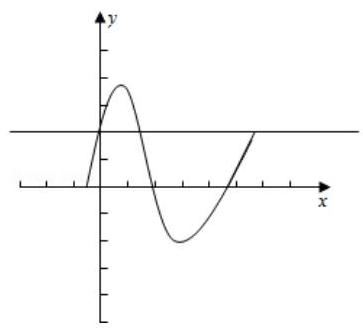
\includegraphics[max width=0.3\textwidth]{images/bo_d5jma53ef24c73bll4ig_110_1090_383_363_330_0.jpg}
\end{center}
\hspace*{3em} 

【解析】 \(\sin x + \sqrt{3}\cos x = 2\left( {\frac{1}{2}\sin x + \frac{\sqrt{3}}{2}\cos x}\right)  = 2\sin \left( {x + \frac{\pi }{3}}\right)  = a\) ,

如图方程的解即为直线与三角函数图象的交点,

在 \(\left\lbrack  {0,{2\pi }}\right\rbrack\) 上，当 \(a = \sqrt{3}\) 时，直线与三角函数图象恰有三个交点，

令 \(\sin \left( {x + \frac{\pi }{3}}\right)  = \frac{\sqrt{3}}{2},x + \frac{\pi }{3} = {2k\pi } + \frac{\pi }{3}\) ,

即 \(x = {2k\pi }\) ,或 \(x + \frac{\pi }{3} = {2k\pi } + \frac{2\pi }{3}\) ,即 \(x = {2k\pi } + \frac{\pi }{3}\) ,

所以此时 \({x}_{1} = 0,{x}_{2} = \frac{\pi }{3},{x}_{3} = {2\pi }\) ,

所以 \({x}_{1} + {x}_{2} + {x}_{3} = 0 + \frac{\pi }{3} + {2\pi } = \frac{7\pi }{3}\) .

【例题】8. (2012 上海秋考) 设 \({a}_{n} = \frac{1}{n}\sin \frac{n\pi }{25},{S}_{n} = {a}_{1} + {a}_{2} + \cdots  + {a}_{n}\) ,在 \({S}_{1},{S}_{2},\cdots ,{S}_{100}\) 中,正数的个数是 ( )

A. 25 B. 50 C. 75 D. 100

【答案】D

【解析】由于 \(f\left( n\right)  = \sin \frac{n\pi }{25}\) 的周期 \(T = {50}\) ,由正弦函数性质得

\({a}_{1},{a}_{2},\cdots ,{a}_{24} > 0,{a}_{25} = 0,{a}_{26},{a}_{27},\cdots ,{a}_{49} < 0,{a}_{50} = 0,\)

且 \(\sin \frac{26\pi }{25} =  - \sin \frac{\pi }{25},\sin \frac{27\pi }{25} =  - \sin \frac{2\pi }{25},\cdots\) 但是 \(f\left( n\right)  = \frac{1}{n}\) 单调递减,

\({a}_{26},\cdots ,{a}_{49}\) 都为负数,但是 \(\left| {a}_{26}\right|  < {a}_{1},\left| {a}_{27}\right|  < {a}_{2},\cdots ,\left| {a}_{49}\right|  < {a}_{24}\)

所以 \({S}_{1},{S}_{2},\cdots ,{S}_{25}\) 中都为正,而 \({S}_{26},{S}_{27},\cdots ,{S}_{50}\) 都为正,

同理 \({S}_{1},{S}_{2},\cdots ,{S}_{75}\) 都为正, \({S}_{1},{S}_{2},\cdots ,{S}_{75},\cdots ,{S}_{100}\) 都为正,故选 \(D\) . 2025 版上海高考真题及模拟训练合集

\section*{2. 模拟练习}

【练习】1. (2025 届交附) 已知函数 \(y = A\sin \left( {{\omega x} + \varphi }\right) \left( {A > 0,\omega  > 0,0 \leq  \varphi  < {2\pi }}\right)\) 的图像与直线 \(y = \; b\left( {0 < b < A}\right)\) 的三个相邻交点的横坐标依次是1,2,4,则 \(\varphi  =\) \_\_\_\_\_

【答案】 \(\frac{3\pi }{2}\)

【解析】因为三个交点的横坐标依次是是1,2,4,所以 \(T = 4 - 1 = 3\) ,那么 \(\omega  = \frac{2\pi }{T} = \frac{2\pi }{3}\)

又因为 \(y = b > 0\) ，所以当 \(x = \frac{1 + 2}{2} = \frac{3}{2}\) 时，函数取到最大值，

所以 \(\frac{2\pi }{3} \times  \frac{3}{2} + \varphi  = \frac{\pi }{2} + {2k\pi },\left( {k \in  Z}\right)\) ,解得 \(\varphi  =  - \frac{\pi }{2} + {2k\pi },\left( {k \in  Z}\right)\)

因为 \(\varphi  \in  \lbrack 0,{2\pi })\) ,所以取 \(k = 1,\varphi  = \frac{3\pi }{2}\)

【练习】2. 若集合 \(A = \left\{  {x\left| {\;x = \sin \frac{2\pi }{2023} + \sin \frac{4\pi }{2023} + \sin \frac{6\pi }{2023} + \cdots  + \sin \frac{2k\pi }{2023}}\right. ,k \in  Z,k > 0}\right\}\) ,则集合 \(A\) 的元素个数为 ( )

A. 1011 B. 1012 C. 2022 D. 2023

【答案】 \(A\)

【解析】当 \(0 < k \leq  {1011},k \in  Z\) 时, \(\frac{2k\pi }{2023} \in  \left( {0,\pi }\right)\) ,此时 \(\sin \frac{2k\pi }{2023} \in  \left( {0,1}\right)\) ;

又因为 2023 为奇数, \({2k}\) 为偶数,且 \(\frac{2k\pi }{2023}\) 中的任意两组角都不关于 \(\frac{\pi }{2}\) 对称,

所以 \(\sin \frac{2k\pi }{2023}\) 的取值各不相同,

因此当 \(0 < k \leq  {1011},k \in  Z\) 时,集合 \(A\) 中 \(x\) 的取值会随着 \(k\) 的增大而增大,

所以当 \(k = {1011}\) 时,集合 \(A\) 中有 1011 个元素;

当 \(k = {1012}\) 时,易得 \(x = \sin \frac{2\pi }{2023} + \sin \frac{4\pi }{2023} + \cdots  + \sin \frac{2022\pi }{2023} + \sin \frac{2024\pi }{2023}\)

\(= \sin \frac{2\pi }{2023} + \sin \frac{4\pi }{2023} + \cdots  + \sin \frac{2022\pi }{2023} + \sin \left( {\pi  + \frac{\pi }{2023}}\right)\)

\(= \sin \frac{2\pi }{2023} + \sin \frac{4\pi }{2023} + \cdots  + \sin \frac{2022\pi }{2023} - \sin \frac{\pi }{2023}\) ,

易得 \(\sin \frac{2022\pi }{2023} = \sin \frac{\pi }{2023}\) ,

所以 \(x = \sin \frac{2\pi }{2023} + \sin \frac{4\pi }{2023} + \cdots  + \sin \frac{2022\pi }{2023} + \sin \frac{2024\pi }{2023}\)

\(= \sin \frac{2\pi }{2023} + \sin \frac{4\pi }{2023} + \cdots  + \sin \frac{2020\pi }{2023}\) ,

即 \(k = {1012}\) 时 \(x\) 的取值与 \(k = {1010}\) 时的取值相同,

由集合元素的互异性得, \(k = {1012}\) 时并没有增加集合中的元素个数,

以此类推得当 \(k \geq  {1012}\) 时,集合 \(A\) 中的元素个数并没有随着 \(k\) 的增大而增加,

所以集合 \(A\) 的元素个数为 1011 个. 故选 \(A\) .

【练习】3. (2024 届华二) 在 \(\bigtriangleup  {ABC}\) 中，已知 \(\sin A = a,\cos B = \frac{3}{5}\) ，若 \(\cos C\) 有唯一值，则实数 \(a\) 的取值范围为 ( )

A. \(\left( {0,\frac{3}{5}}\right\rbrack   \cup  \{ 1\}\) B. \(\left( {0,\frac{4}{5}}\right\rbrack\) C. \(\left\lbrack  {\frac{4}{5},1}\right\rbrack\) D. \(\left( {0,\frac{4}{5}}\right\rbrack   \cup  \{ 1\}\)

【答案】 \(D\)

【解析】由 \(\cos B = \frac{3}{5}\) 得角 \(B\) 唯一确定,且 \(\sin B = \frac{4}{5}\) ,

若 \(a \leq  \frac{4}{5}\) ,则 \(\sin A \leq  \sin B\) ,由正弦定理得 \(a \leq  b\) ,从而角 \(A\) 为锐角,

从而角 \(A\) 唯一确定，所以角 \(C\) 唯一，则 \(\cos C\) 有唯一值；

若 \(a = 1\) ,则 \(A = \frac{\pi }{2}\) ,从而角 \(A\) 唯一确定,所以角 \(C\) 唯一,则 \(\cos C\) 有唯一值;

故选 \(D\) .

【练习】4. 已知 \(\omega  \in  \mathbb{R},\varphi  \in  \lbrack 0,{2\pi })\) ,若对任意实数 \(x\) 均有 \(\sin x \geq  \cos \left( {{\omega x} + \varphi }\right)\) ,则满足条件的有序实数对 \(\left( {\omega ,\varphi }\right)\) 的个数为 ( )

A. 1 个 B. 2 个 C. 3 个 D. 无数个

【答案】 \(C\)

【解析】当 \(x \in  \mathbb{R}\) 时, \(\sin x \in  \left\lbrack  {-1,1}\right\rbrack  ,\cos \left( {{\omega x} + \varphi }\right)  \in  \left\lbrack  {-1,1}\right\rbrack\) .

为了保证 \(\sin x\) 始终大于 \(\cos \left( {{\omega x} + \varphi }\right)\) (从图像上看, \(\sin x\) 始终高于 \(\cos \left( {{\omega x} + \varphi }\right)\) )

必须满足: \(\sin x =  - 1 \geq  \cos \left( {{\omega x} + \varphi }\right)  =  - 1,\sin x = 1 \geq  \cos \left( {{\omega x} + \varphi }\right)  = 1\) ,

即 \(\sin x\) 和 \(\cos \left( {{\omega x} + \varphi }\right)\) 同时取到最值 (图形重叠), \(\therefore \sin x = \cos \left( {{\omega x} + \varphi }\right)\) 恒等.

讨论: 当 \(\omega  = 1,\sin x = \cos \left( {{\omega x} + \varphi }\right)\) ,令 \(x = 0 \Rightarrow  \cos \varphi  = 0 \Rightarrow  \varphi  = \frac{\pi }{2}\) 或 \(\frac{3\pi }{2}\) .

经检验, \(\varphi  = \frac{\pi }{2}\) 舍,即 \(\left( {\omega ,\varphi }\right)  = \left( {1,\frac{3\pi }{2}}\right)\) 满足;

当 \(\omega  =  - 1,\sin x = \cos \left( {-x + \varphi }\right)\) ,令 \(x = 0 \Rightarrow  \cos \varphi  = 0 \Rightarrow  \varphi  = \frac{\pi }{2}\) 或 \(\frac{3\pi }{2}\)

经检验, \(\varphi  = \frac{3\pi }{2}\) 舍,即 \(\left( {\omega ,\varphi }\right)  = \left( {-1,\frac{\pi }{2}}\right)\) 满足;

注意: 当 \(\omega  = 0\) 时, \(\sin x \geq  \cos \varphi\) 恒成立,即 \(\cos \varphi  =  - 1 \Rightarrow  \varphi  = \pi\) ,此时 \(\left( {\omega ,\varphi }\right)  = \left( {0,\pi }\right)\) 满足.

综上所述: \(\left( {\omega ,\varphi }\right)  = \left( {1,\frac{3\pi }{2}}\right)\) 或 \(\left( {\omega ,\varphi }\right)  = \left( {-1,\frac{\pi }{2}}\right)\) 或 \(\left( {\omega ,\varphi }\right)  = \left( {0,\pi }\right)\) ,共 3 对,选 \(C\) .

【练习】5. (2025 届复附) 设函数 \(f\left( x\right)  = {\sin }^{4}\frac{kx}{10} + {\cos }^{4}\frac{kx}{10}\) ,其中 \(k\) 是一个正整数. 若对任意实数 \(a\) ,均有 \(\{ f\left( x\right)  \mid  a < x < a + 1\}  = \{ f\left( x\right)  \mid  x \in  R\}\) ,则 \(k\) 的最小值为\_\_\_\_\_

【答案】 16

【解析】 \(f\left( x\right)  = {\left( {\sin }^{2}\frac{kx}{10} + {\cos }^{2}\frac{kx}{10}\right) }^{2} - 2{\sin }^{2}\frac{kx}{10}{\cos }^{2}\frac{kx}{10} = 1 - \frac{1}{2}{\sin }^{2}\frac{kx}{5} = \frac{1}{4}\cos \frac{2kx}{5} + \frac{3}{4}\) ,

其中当且仅当 \(x = \frac{5m\pi }{k}\left( {m \in  Z}\right)\) 时, \(f\left( x\right)\) 取到最大值,

由题意得任意一个长为 1 的开区间 \(\left( {a,a + 1}\right)\) 至少包含一个最大值点,

从而 \(\frac{5\pi }{k} < 1\) ,即 \(k > {5\pi }\) ;

反之,当 \(k > {5\pi }\) 时,任意一个开区间 \(\left( {a,a + 1}\right)\) 均包含 \(f\left( x\right)\) 的一个完整周期,

此时 \(\{ f\left( x\right)  \mid  a < x < a + 1\}  = \{ f\left( x\right)  \mid  x \in  R\}\) 成立,

综上,正整数 \(k\) 的最小值为 \(\left\lbrack  {5\pi }\right\rbrack   + 1 = {16}\)

【练习】6. 若分段函数 \(f\left( x\right)  = \left\{  \begin{array}{ll} 3\sin {2x}, & x \leq  0 \\  {2}^{x} - 3, & x > 0 \end{array}\right.\) ,将函数 \(y = \left| {f\left( x\right)  - f\left( a\right) }\right| ,x \in  \left\lbrack  {m,n}\right\rbrack\) 的最大值记作 \({Z}_{a}\left\lbrack  {m,n}\right\rbrack\) ，那么当 \(- 2 \leq  m \leq  2\) 时， \({Z}_{2}\left\lbrack  {m,m + 4}\right\rbrack\) 的取值范围是\_\_\_\_\_；

【答案】 \(\left\lbrack  {4,{60}}\right\rbrack\)

【解析】由 \(f\left( x\right)  = \left\{  \begin{array}{l} 3\sin {2x},x \leq  0 \\  {2}^{x} - 3,x > 0 \end{array}\right.\) ,得 \(f\left( 2\right)  = 1\) ,

则 \(y = \left| {f\left( x\right)  - f\left( a\right) }\right|  = \left| {f\left( x\right)  - 1}\right|\) ,

\begin{center}
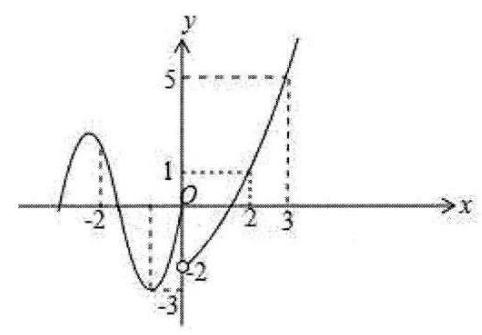
\includegraphics[max width=0.4\textwidth]{images/bo_d5jma53ef24c73bll4ig_113_298_375_482_335_0.jpg}
\end{center}
\hspace*{3em} 

作出函数 \(f\left( x\right)\) 的图象如图所示:

当 \(- 2 \leq  m \leq   - 1\) 时, \({\left| f\left( x\right)  - 1\right| }_{\max } = \left| {\left( {-3}\right)  - 1}\right|  = 4\) ;

当 \(m >  - 1\) 时, \(m + 4 > 3,{2}^{m + 4} - 3 - 1 = {2}^{m + 4} - 4 > 4\) ,

\(\therefore\) 当 \(- 1 < m \leq  2\) 时, \({Z}_{a}\left\lbrack  {m,m + 4}\right\rbrack   = {2}^{m + 4} - 4\) ,

则 \({Z}_{2}\left\lbrack  {m,m + 4}\right\rbrack\) 的最大值为 \({2}^{6} - 4 = {60}\) .

故 \({Z}_{2}\left\lbrack  {m,m + 4}\right\rbrack\) 的取值范围是 \(\left\lbrack  {4,{60}}\right\rbrack\) .

【练习】7. (2024 届七宝)已知 \(k\) 是正整数，且 \(1 \leq  k \leq  {2024}\) ，则满足方程 \(\sin {1}^{ \circ  } + \sin {2}^{ \circ  } + \cdots  + \sin {k}^{ \circ  } = \; \sin {1}^{ \circ  } \cdot  \sin {2}^{ \circ  }\cdots \sin {k}^{ \circ  }\) 的 \(k\) 有\_\_\_\_\_个.

【答案】 11

【解析】由正弦函数性质得 \(\sin {1}^{ \circ  } \cdot  \sin {2}^{ \circ  }\cdots \sin {k}^{ \circ  } < 1\) ,

 \circled{1}  \(k = 1\) ，等式两边成立；

 \circled{2} 等式的两边都为 0 时等式才成立，

\(k = {359},{360},{719},{720},{1079},{1080},{1439},{1440},{1799},{1800}\) 时等式成立.

综上 \(k = 1,{359},{360},{719},{720},{1079},{1080},{1439},{1440},{1799},{1800}\) ,

共 11 个.

【练习】8. 已知函数 \(f\left( x\right)  = \cos {2x}\) 在区间 \(\left\lbrack  {t,t + \frac{\pi }{3}}\right\rbrack  \left( {t \in  R}\right)\) 上的最大值为 \(M\left( t\right)\) ，则 \(M\left( t\right)\) 的最小值为 ( )

A. \(\frac{\sqrt{3}}{2}\) B. \(- \frac{\sqrt{3}}{2}\) C. \(\frac{1}{2}\) D. \(- \frac{1}{2}\)

【答案】 \(D\)

【解析】函数 \(f\left( x\right)  = \cos {2x}\) 的最小正周期为 \(T = \pi\) ,区间 \(\left\lbrack  {t,t + \frac{\pi }{3}}\right\rbrack\) 的长度为 \(\frac{1}{3}\pi  = \frac{1}{3}T\) ,

考虑一个周期内 \(M\left( t\right)\) 的取值情况，

作出 \(f\left( x\right)\) 在区间 \(\left\lbrack  {-\frac{\pi }{4},\frac{3\pi }{4}}\right\rbrack\) 这一个周期内的函数图象,如下所示,

由图象得,当 \(- \frac{\pi }{4} \leq  t < \frac{\pi }{3}\) 时, \(\frac{\pi }{12} \leq  t + \frac{\pi }{3} < \frac{2\pi }{3}\) ,最大值 \(M\left( t\right)  >  - \frac{1}{2}\) ;

\begin{center}
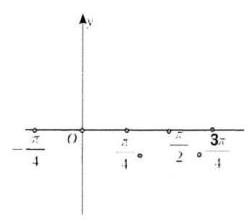
\includegraphics[max width=0.2\textwidth]{images/bo_d5jma53ef24c73bll4ig_114_296_236_251_221_0.jpg}
\end{center}
\hspace*{3em} 

当 \(t = \frac{\pi }{3}\) 时, \(t + \frac{\pi }{3} = \frac{2\pi }{3}\) ,最大值 \(M\left( t\right)  =  - \frac{1}{2}\) ;

当 \(\frac{\pi }{3} < t \leq  \frac{3\pi }{4}\) 时, \(\frac{2\pi }{3} < t + \frac{\pi }{3} \leq  \frac{13\pi }{12}\) ,最大值 \(M\left( t\right)  >  - \frac{1}{2}\) ,

综上, \(M\left( t\right)\) 的最小值为 \(- \frac{1}{2}\) . 故选 \(D\) .

【练习】9. (2024 届华二) 已知函数 \(f\left( x\right)  = \sin \frac{\pi }{2}x\) ,任取 \(t \in  R\) ,记函数 \(f\left( x\right)\) 在 \(\left\lbrack  {t,t + 1}\right\rbrack\) 上的最大值为 \({M}_{t}\) ,最小值为 \({m}_{t}\) ,设 \(h\left( t\right)  = {M}_{t} - {m}_{t}\) ,则函数 \(h\left( t\right)\) 的值域为 ( )

A. \(\left\lbrack  {1 - \frac{\sqrt{2}}{2},1}\right\rbrack\) B. \(\left\lbrack  {1 - \frac{\sqrt{2}}{2},1 + \frac{\sqrt{2}}{2}}\right\rbrack\)

C. \(\left\lbrack  {1 - \frac{\sqrt{2}}{2},\sqrt{2}}\right\rbrack\) D. \(\left\lbrack  {\frac{\sqrt{2}}{2},1 + \frac{\sqrt{2}}{2}}\right\rbrack\)

【答案】 \(C\)

【解析】因为 \(h\left( {t + 4}\right)  = {M}_{t + 4} - {m}_{t + 4}\) ,

其中 \({M}_{t + 4}\text{ 、 }{m}_{t + 4}\) 分别是指 \(f\left( x\right)\) 在区间 \(\left\lbrack  {t + 4,t + 5}\right\rbrack\) 上的最大值和最小值,

因为 \(f\left( x\right)\) 的周期 \(T = \frac{2\pi }{\frac{\pi }{2}} = 4\) ,

所以 \(f\left( x\right)\) 在区间 \(\left\lbrack  {t + 4,t + 5}\right\rbrack\) 的图象与在区间 \(\left\lbrack  {t,t + 1}\right\rbrack\) 上的图象完全相同,

故 \({M}_{t + 4} = {M}_{t},{m}_{t + 4} = {m}_{t}\) ,故 \(h\left( {t + 4}\right)  = h\left( t\right)\) ,即 \(h\left( t\right)\) 是周期为 4 的函数,

故 \(h\left( t\right) ,t \in  R\) 的值域与 \(h\left( t\right) ,t \in  \left\lbrack  {-2,2}\right\rbrack\) 时的值域相同;

又 \(f\left( x\right)\) 在 \(\left\lbrack  {-2, - 1}\right\rbrack\) 严格减, \(\left\lbrack  {-1,1}\right\rbrack\) 严格增,在 \(\left\lbrack  {1,2}\right\rbrack\) 严格减,

故当 \(t \in  \left\lbrack  {-2, - \frac{3}{2}}\right)\) 时， \(f\left( x\right)\) 在区间 \(\left\lbrack  {t,t + 1}\right\rbrack\) 上的最大值为 \(f\left( t\right)  = \sin \frac{\pi }{2}t\) ，

最小值为 -1,此时 \(h\left( t\right)  = \sin \frac{\pi }{2}t + 1\) ;

当 \(t \in  \left\lbrack  {-\frac{3}{2}, - 1}\right)\) 时, \(f\left( x\right)\) 在区间 \(\left\lbrack  {t,t + 1}\right\rbrack\) 上的最大值

为 \(f\left( {t + 1}\right)  = \sin \left( {\frac{\pi }{2}t + \frac{\pi }{2}}\right)  = \cos \frac{\pi }{2}t\) ,最小值为 -1,此时 \(h\left( t\right)  = \cos \frac{\pi }{2}t + 1\) ;

当 \(t \in  \lbrack  - 1,0)\) 时,在区间 \(\left\lbrack  {t,t + 1}\right\rbrack\) 上的最大值为,最小值为 \(f\left( t\right)  = \sin \frac{\pi }{2}t\) ,

此时 \(h\left( t\right)  = \cos \frac{\pi }{2}t - \sin \frac{\pi }{2}t =  - \sqrt{2}\sin \left( {\frac{\pi }{2}t - \frac{\pi }{4}}\right)\) ;

当 \(t \in  \left\lbrack  {0,\frac{1}{2}}\right)\) 时, \(f\left( x\right)\) 在区间 \(\left\lbrack  {t,t + 1}\right\rbrack\) 上的最大值为 1,

最小值为 \(f\left( t\right)  = \sin \frac{\pi }{2}t\) ,此时 \(h\left( t\right)  = 1 - \sin \frac{\pi }{2}t\) ;

当 \(t \in  \left\lbrack  {\frac{1}{2},1}\right)\) 时, \(f\left( x\right)\) 在区间 \(\left\lbrack  {t,t + 1}\right\rbrack\) 上的最大值为 1,

最小值为 \(f\left( {t + 1}\right)  = \cos \frac{\pi }{2}t\) ,此时 \(h\left( t\right)  = 1 - \cos \frac{\pi }{2}t\) ;

当 \(t \in  \left\lbrack  {1,2}\right\rbrack\) 时, \(f\left( x\right)\) 在区间 \(\left\lbrack  {t,t + 1}\right\rbrack\) 上的最大值为 \(f\left( t\right)  = \sin \frac{\pi }{2}t\) , 2025 版上海高考真题及模拟训练合集

最小值为 \(f\left( {t + 1}\right)  = \cos \frac{\pi }{2}t\) ,此时 \(h\left( t\right)  = \sin \frac{\pi }{2}t - \cos \frac{\pi }{2}t = \sqrt{2}\sin \left( {\frac{\pi }{2}t - \frac{\pi }{4}}\right)\) ;

故 \(h\left( t\right)\) 在 \(\left\lbrack  {-2,2}\right\rbrack\) 的函数图象如下所示:

\begin{center}
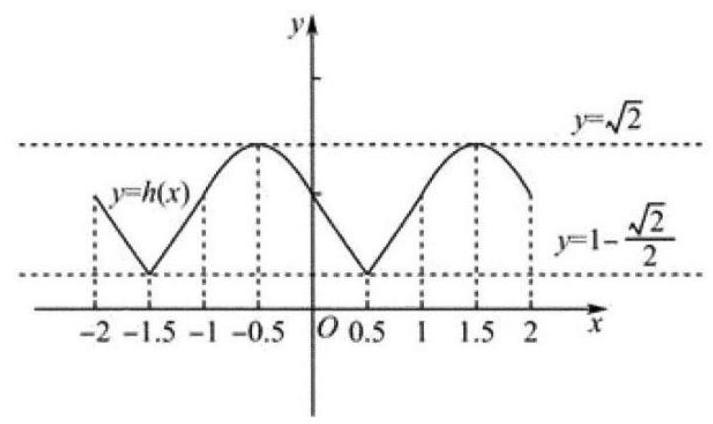
\includegraphics[max width=0.6\textwidth]{images/bo_d5jma53ef24c73bll4ig_115_323_351_713_424_0.jpg}
\end{center}
\hspace*{3em} 

数形结合得 \(h\left( t\right)\) 的值域为 \(\left\lbrack  {1 - \frac{\sqrt{2}}{2},\sqrt{2}}\right\rbrack\) . 故选 \(C\) .

【练习】10. (2024 届格致) 对任意闭区间 \(I\) ，用 \({M}_{I}\) 表示函数 \(y = \sin x\) 在 \(I\) 上的最大值，若有且仅有一个正数 \(a\) 使得 \({M}_{\left\lbrack  0,a\right\rbrack  } = k{M}_{\left\lbrack  a,2a\right\rbrack  }\) 成立，则实数 \(k\) 的取值范围是\_\_\_\_\_.

【答案】 \(\left( {\frac{1}{2},1}\right)\)

【解析】 \circled{1}  当 \(a \in  \left\lbrack  {0,\frac{\pi }{4}}\right\rbrack\) 时, \({2a} \in  \left\lbrack  {0,\frac{\pi }{2}}\right\rbrack  ,{M}_{\left\lbrack  0,a\right\rbrack  } = \sin a,{M}_{\left\lbrack  a,2a\right\rbrack  } = \sin {2a}\) ,

由 \({M}_{\left\lbrack  0,a\right\rbrack  } = k{M}_{\left\lbrack  a,2a\right\rbrack  }\) ,得 \(\sin a = k\sin {2a}\) ,所以 \(k = \frac{1}{2\cos a}\) ;

 \circled{2}  当 \(a \in  \left\lbrack  {\frac{\pi }{4},\frac{\pi }{2}}\right\rbrack\) 时， \({2a} \in  \left\lbrack  {\frac{\pi }{2},\pi }\right\rbrack  ,{M}_{\left\lbrack  0,a\right\rbrack  } = \sin a,{M}_{\left\lbrack  a,2a\right\rbrack  } = 1\) ，

由 \({M}_{\left\lbrack  0,a\right\rbrack  } = k{M}_{\left\lbrack  a,2a\right\rbrack  }\) ,得 \(k = \sin a\) ;

 \circled{3}  当 \(a \in  \left\lbrack  {\frac{\pi }{2},\pi }\right\rbrack\) 时， \({2a} \in  \left\lbrack  {\pi ,{2\pi }}\right\rbrack  ,{M}_{\left\lbrack  0,a\right\rbrack  } = 1,{M}_{\left\lbrack  a,{2a}\right\rbrack  } = \sin a\) ，

由 \({M}_{\left\lbrack  0,a\right\rbrack  } = k{M}_{\left\lbrack  a,2a\right\rbrack  }\) ,得 \(1 = k\sin a\) ,所以 \(k = \frac{1}{\sin a}\) ;

 \circled{4}  当 \(a \in  \left\lbrack  {\pi ,\frac{5\pi }{4}}\right\rbrack\) 时， \({2a} \in  \left\lbrack  {{2\pi },\frac{5}{2}\pi }\right\rbrack\) ， \({M}_{\left\lbrack  0,a\right\rbrack  } = 1\) ， \({M}_{\left\lbrack  a,2a\right\rbrack  } = \sin {2a}\) ，

由 \({M}_{\left\lbrack  0,a\right\rbrack  } = k{M}_{\left\lbrack  a,2a\right\rbrack  }\) ,得 \(1 = k\sin {2a}\) ,所以 \(k = \frac{1}{\sin {2a}}\) ,

 \circled{5}  当 \(a \in  \left\lbrack  {\frac{5\pi }{4}, + \infty }\right\rbrack\) 时, \({2a} \in  \left\lbrack  {\frac{5}{2}\pi ,{3\pi }}\right\rbrack  ,{M}_{\left\lbrack  0,a\right\rbrack  } = 1,{M}_{\left\lbrack  a,2a\right\rbrack  } = 1\)

由 \({M}_{\left\lbrack  0,a\right\rbrack  } = k{M}_{\left\lbrack  a,2a\right\rbrack  }\) ,得 \(k = 1\) ,

\[
\text{ 所以 }k = \left\{  \begin{array}{l} \frac{1}{2\cos a},a \in  \left\lbrack  {0,\frac{\pi }{4}}\right\rbrack  \\  \sin a,a \in  \left\lbrack  {\frac{\pi }{4},\frac{\pi }{2}}\right\rbrack  \\  \frac{1}{\sin a},a \in  \left\lbrack  {\frac{\pi }{2},\pi }\right\rbrack  \\  \frac{1}{\sin {2a}},a \in  \left\lbrack  {\pi ,\frac{5\pi }{4}}\right\rbrack  \\  \tan a \in  \left\lbrack  {\frac{5\pi }{4}, + \infty }\right\rbrack   \end{array}\right.
\]

\begin{center}
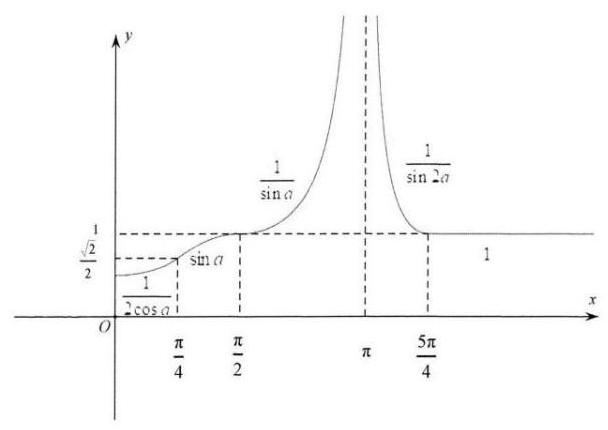
\includegraphics[max width=0.5\textwidth]{images/bo_d5jma53ef24c73bll4ig_115_295_1667_608_430_0.jpg}
\end{center}
\hspace*{3em} 

作出图像,得实数 \(k\) 的取值范围是 \(\left( {\frac{1}{2},1}\right)\) . 2025 版上海高考真题及模拟训练合集

\section*{板块二: 压轴客观题}

1. 真题回顾

【例题】1. (2025 上海春考) 已知 \(a \in  \mathbb{R}\) ,不等式 \(\left\lbrack  {\tan \left( {\frac{\pi }{6}x}\right)  - a}\right\rbrack   \cdot  \left\lbrack  {\tan \left( {\frac{\pi }{6}x}\right)  - a - 1}\right\rbrack   < 0\) 在 \(\left( {0,{2025}}\right)\) 中的整数解有 \(m\) 个，关于 \(m\) 的个数，以下不可能的是( ).

A. 0 B. 338 C. 674 D. 1012

【答案】 \(D\)

【解析】数形结合: 先解不等式,易得 \(\tan \left( {\frac{\pi }{6}x}\right)  \in  \left( {a,a + 1}\right)\) ,区间跨度为 1 .

分析其在 \(\left( {0,{2025}}\right)\) 中的整数解数量时,自然要先考虑 \(f\left( x\right)  = \tan \left( {\frac{\pi }{6}x}\right)\) 的图像及其性质:

\(f\left( x\right)  = \tan \left( {\frac{\pi }{6}x}\right)\) 的最小正周期为 6,定义域为 \(\{ x \mid  x \neq  3 + {6k},k \in  \mathbb{Z}\}\) ,在一个周期内的整数取值: \(f\left( {-2}\right)  =  - \sqrt{3} \approx   - {1.732},f\left( {-1}\right)  =  - \frac{\sqrt{3}}{3} \approx   - {0.577},f\left( 0\right)  = 0,f\left( 1\right)  = \frac{\sqrt{3}}{3} \approx  {0.577},f\left( 2\right)  = \sqrt{3} \; \approx  {1.732}\) .

由于 \({2025} = 6 \times  {337} + 3\) ,我们可将 \(\left( {0,{2025}}\right)\) 拆分为: \(\left( {0,3}\right) ,\left( {3,9}\right) ,\left( {9,{15}}\right) \cdots \left( {{2019},{2025}}\right)\) . 接下来我们先分析 \(f\left( x\right)  = \tan \left( {\frac{\pi }{6}x}\right)\) 在一个周期内可能的整数解数量,进而推算到 \(\left( {0,{2025}}\right)\) 内的整数解个数。由于 \(\left( {a,a + 1}\right)\) 的区间长度为 1,因而分类讨论如下:

当 \(a > \sqrt{3}\) 时,在 \(\left( {0,3}\right)\) 内满足 \(\tan \left( {\frac{\pi }{6}x}\right)  \in  \left( {a,a + 1}\right)\) 的整数解为 0 个,在之后每个周期内满足 \(\tan \left( {\frac{\pi }{6}x}\right)  \in  \left( {a,a + 1}\right)\) 的整数解也为 0 个,此时在 \(\left( {0,{2025}}\right)\) 内的整数解也为 0 个;

\begin{center}
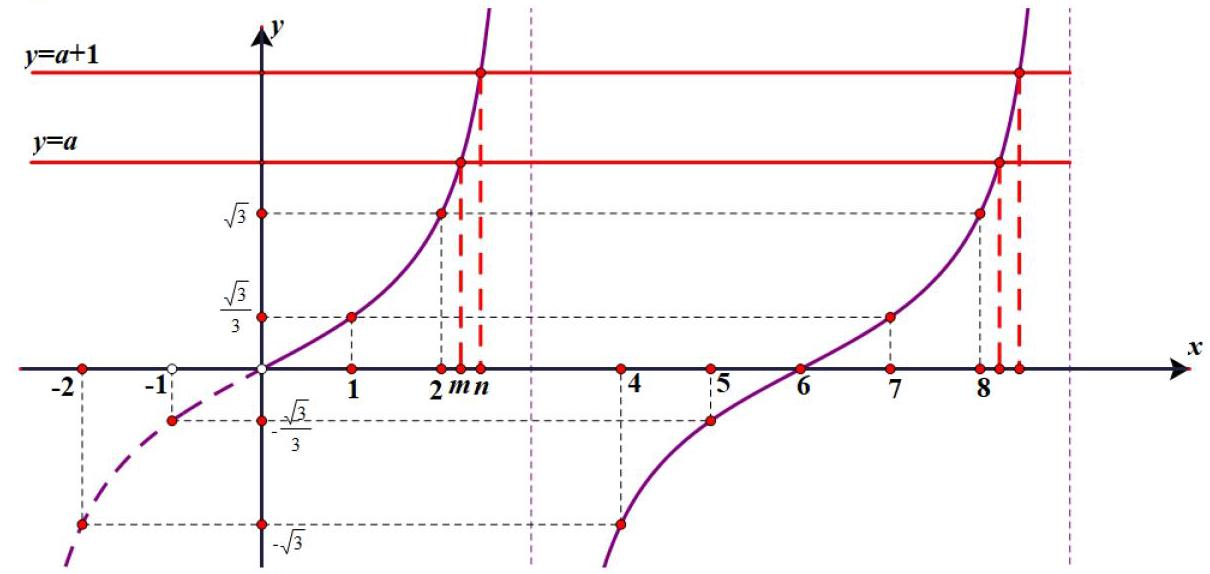
\includegraphics[max width=1.0\textwidth]{images/bo_d5jma53ef24c73bll4ig_117_324_1163_1210_574_0.jpg}
\end{center}
\hspace*{3em} 

当 \(a + 1 > \sqrt{3} > a > \frac{\sqrt{3}}{3}\) 时,在 \(\left( {0,3}\right)\) 内满足 \(\tan \left( {\frac{\pi }{6}x}\right)  \in  \left( {a,a + 1}\right)\) 的整数解为 1 个,在之后每个周期内满足 \(\tan \left( {\frac{\pi }{6}x}\right)  \in  \left( {a,a + 1}\right)\) 的整数解也为 1 个，此时在 \(\left( {0,{2025}}\right)\) 中整数解数量为 \(1 \times \; {337} + 1 = {338}\)

2025 版上海高考真题及模拟训练合集

\begin{center}
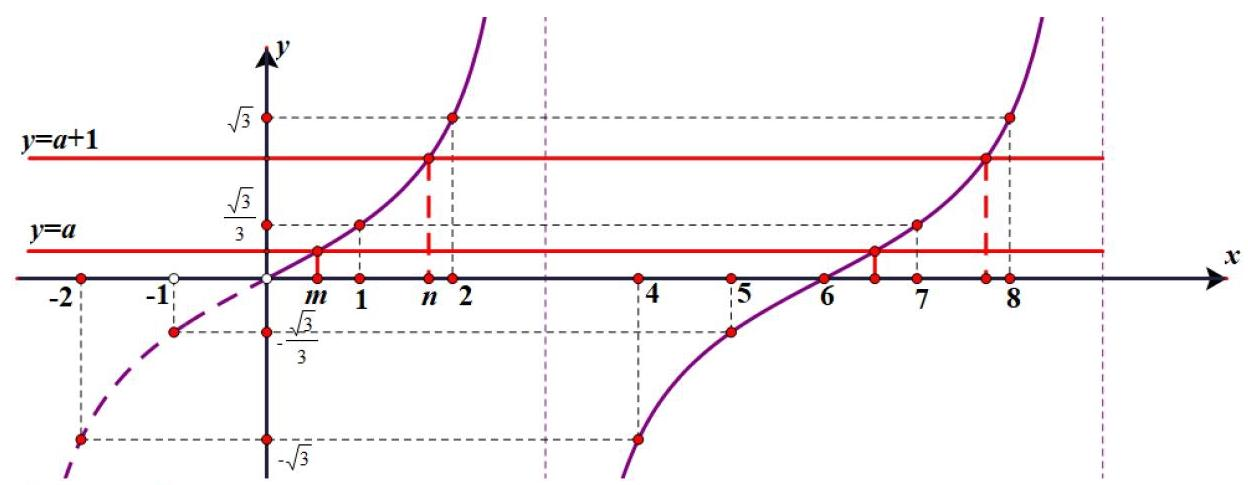
\includegraphics[max width=1.0\textwidth]{images/bo_d5jma53ef24c73bll4ig_118_309_223_1248_485_0.jpg}
\end{center}
\hspace*{3em} 

当 \(\left\{  \begin{array}{l} a + 1 > \frac{\sqrt{3}}{3} \\  0 > a \end{array}\right.\) 即 \(0 > a > \frac{\sqrt{3}}{3} - 1\) 时,在 \(\left( {0,3}\right)\) 内满足 \(\tan \left( {\frac{\pi }{6}x}\right)  \in  \left( {a,a + 1}\right)\) 的整数解为 1 个,

在之后每个周期内满足 \(\tan \left( {\frac{\pi }{6}x}\right)  \in  \left( {a,a + 1}\right)\) 的整数解为 2 个,此时在 \(\left( {0,{2025}}\right)\) 中整数解数量

为 \(2 \times  {337} + 1 = {675}\) ;

\begin{center}
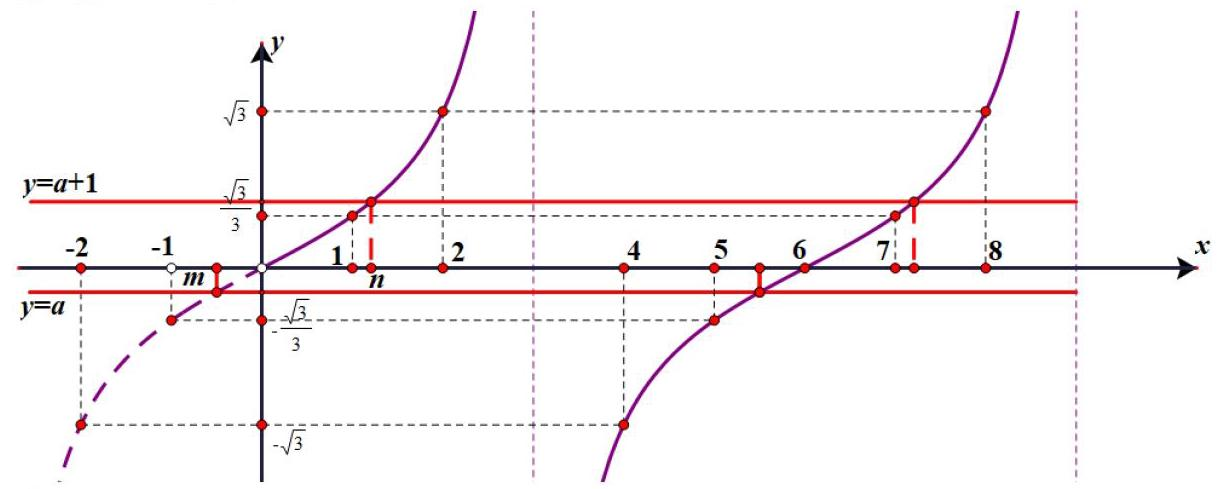
\includegraphics[max width=1.0\textwidth]{images/bo_d5jma53ef24c73bll4ig_118_308_923_1221_489_0.jpg}
\end{center}
\hspace*{3em} 

当 \(\left\{  \begin{array}{l} a + 1 > 0 \\   - \frac{\sqrt{3}}{3} > a \end{array}\right.\) 即 \(- \frac{\sqrt{3}}{3} > a >  - 1\) 时,在 \(\left( {0,3}\right)\) 内满足 \(\tan \left( {\frac{\pi }{6}x}\right)  \in  \left( {a,a + 1}\right)\) 的整数解为 0 个,在之后每个周期内满足 \(\tan \left( {\frac{\pi }{6}x}\right)  \in  \left( {a,a + 1}\right)\) 的整数解为 2 个,此时在 \(\left( {0,{2025}}\right)\) 中整数解数量为 \(2 \times  {337} = {674}\)

\begin{center}
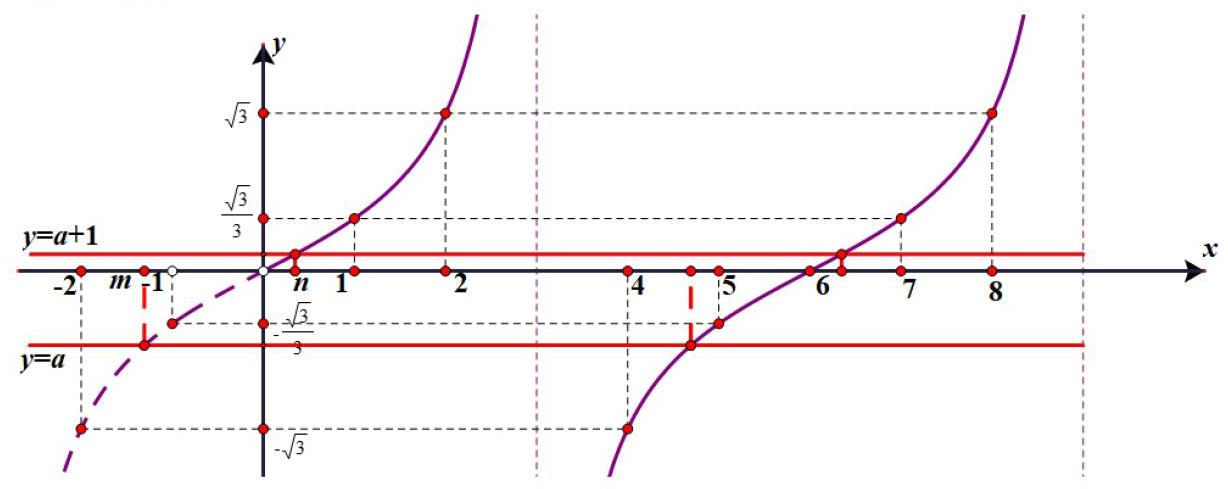
\includegraphics[max width=1.0\textwidth]{images/bo_d5jma53ef24c73bll4ig_118_312_1623_1228_489_0.jpg}
\end{center}
\hspace*{3em} 

因此四个选项中,唯独不可能是 1012 个,故选 \(D\) .

【例题】2. (2021 上海春考) 已知 \(\theta  > 0\) ，存在实数 \(\varphi\) ，使得对任意 \(n \in  {N}^{ * }\) ， \(\cos \left( {{n\theta } + \varphi }\right)  < \frac{\sqrt{3}}{2}\) ，则 \(\theta\) 的最小值是\_\_\_\_\_.

【答案】 \(\frac{2\pi }{5}\)

\begin{center}
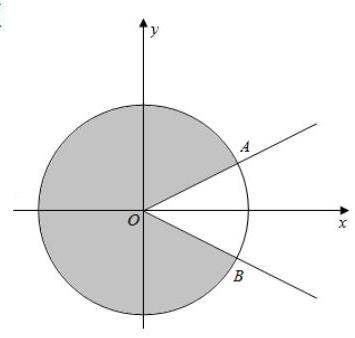
\includegraphics[max width=0.3\textwidth]{images/bo_d5jma53ef24c73bll4ig_119_1099_480_355_338_0.jpg}
\end{center}
\hspace*{3em} 

【解析】在单位圆中分析,由题意得 \({n\theta } + \varphi\) 的终边要落在图中阴影部分区域

(其中 \(\angle {AOx} = \angle {BOx} = \frac{\pi }{6}\) ),

所以 \(\theta  > \angle {AOB} = \frac{\pi }{3}\) ,因为对任意 \(n \in  {N}^{ * }\) 都成立,

所以 \(\frac{2\pi }{\theta } \in  {N}^{ * }\) ,即 \(\theta  = \frac{2\pi }{k},k \in  {N}^{ * }\) ,

同时 \(\theta  > \frac{\pi }{3}\) ，所以 \(\theta\) 的最小值为 \(\frac{2\pi }{5}\) .

【注】以上仅为简单分析, 下面附上严格证明, 变式题和原理

\(\cos \left( {{n\theta } + \varphi }\right)  \geq  \frac{\sqrt{3}}{2} \Leftrightarrow  {2k\pi } - \frac{\pi }{6} \leq  {n\theta } + \varphi  \leq  {2k\pi } + \frac{\pi }{6},k \in  Z\)

所以题目的条件可转化为: 对任意正整数 \(n\) 和任意整数 \(k\) ,

都有 \({n\theta } + \varphi  \notin  \left\lbrack  {{2k\pi } - \frac{\pi }{6},{2k\pi } + \frac{\pi }{6}}\right\rbrack  ,k \in  Z\)

 \circled{1} 先证: \(\theta  > \frac{\pi }{3}\) (反证法)

假设 \(\theta  \leq  \frac{\pi }{3}\) ，必存在整数 \(k\) ，使得 \(\theta  + \varphi  < {2k\pi } - \frac{\pi }{6}\) ，也必存在正整数 \(n\) ，

使得 \({n\theta } + \varphi  < {2k\pi } - \frac{\pi }{6} \leq  \left( {n + 1}\right) \theta  + \varphi\) ,

则 \(\left( {n + 1}\right) \theta  + \varphi  = {n\theta } + \varphi  + \theta  < {2k\pi } - \frac{\pi }{6} + \frac{\pi }{3} = {2k\pi } + \frac{\pi }{6}\) ,矛盾,

所以 \(\theta  > \frac{\pi }{3}\)

 \circled{2}  当 \(\theta  = \frac{2\pi }{5}\) 时，取 \(\varphi  =  - \frac{\pi }{5}\) ，易得对任意正整数 \(n\) ， \(\cos \left( {{n\theta } + \varphi }\right)\) 恰好取

\(\cos \frac{\pi }{5},\cos \frac{3\pi }{5},\cos \frac{5\pi }{5},\cos \frac{7\pi }{5},\cos \frac{9\pi }{5}\) 这 5 个值,它们均小于 \(\frac{\sqrt{3}}{2}\) ,符合题意

 \circled{3}  假设存在 \(\theta ,\frac{\pi }{3} < \theta  < \frac{2\pi }{5}\) 符合题意，记 \(\alpha  = \frac{2\pi }{5} - \theta  \in  \left( {0,\frac{\pi }{15}}\right)\) ，

取 \(n = {5m},m \in  {N}^{ * }\) ,则 \(\cos \left( {{n\theta } + \varphi }\right)  = \cos \left( {{5m}\left( {\frac{2\pi }{5} - \alpha }\right)  + \varphi }\right)  = \cos \left( {m \cdot  {5\alpha } - \varphi }\right)\) 对正整数 \(m\) 恒成立,

即对任意正整数 \(m\) 和任意整数 \(k\) ,都有 \(m \cdot  {5\alpha } - \varphi  \notin  \left\lbrack  {{2k\pi } - \frac{\pi }{6},{2k\pi } + \frac{\pi }{6}}\right\rbrack  ,k \in  Z\) , 由 (1) 得 \({5\alpha } > \frac{\pi }{3}\) 即 \(\alpha  > \frac{\pi }{15}\) ,与 \(\alpha  \in  \left( {0,\frac{\pi }{15}}\right)\) 矛盾,

综上所述， \(\theta\) 的最小值是 \(\frac{2\pi }{5}\) 2025 版上海高考真题及模拟训练合集

\section*{2. 模拟练习}

【练习】1. (2025 届复附) 若 \(\cos \left( {{2}^{n} \cdot  x}\right)  < 0\) 对 \(n \in  N\) 均成立，则实数 \(x\) 的取值集合为\_\_\_\_\_

【答案】 \(\left\{  {x\left| {\;x = {2k\pi } \pm  \frac{2\pi }{3}}\right. ,k \in  Z}\right\}\)

【解析】首先,若 \(x\) 是满足条件的实数,则 \(\cos x \leq   - \frac{1}{4}\) . 事实上,若 \(- \frac{1}{4} < \cos x < 0\) ,则 \(\cos {2x} = 2{\cos }^{2}x \; - 1 < 2{\left( -\frac{1}{4}\right) }^{2} - 1 =  - \frac{7}{8}\) ,即 \(\cos {2x} <  - \frac{7}{8}\) ,

于是, \(\cos {4x} = 2{\cos }^{2}{2x} - 1 > 2{\left( -\frac{7}{8}\right) }^{2} - 1 = \frac{49}{32} - 1 = \frac{17}{32} > 0\) ,即 \(\cos {4x} > 0\) ,矛盾!

由上得对任意 \(n \in  N\) ，均有 \(\cos {2}^{n}x \leq   - \frac{1}{4}\) ，

得 \(\left| {\cos {2}^{n}x - \frac{1}{2}}\right|  \geq  \frac{3}{4}\) ，又 \(\left| {\cos {2x} + \frac{1}{2}}\right|  = 2\left| {\cos x + \frac{1}{2}}\right|  \cdot  \left| {\cos x - \frac{1}{2}}\right|\)

\(\geq  2\left| {\cos x + \frac{1}{2}}\right|  \cdot  \frac{3}{4} = \frac{3}{2}\left| {\cos x + \frac{1}{2}}\right|\) ,故 \(\left| {\cos x + \frac{1}{2}}\right|  \leq  \frac{2}{3}\left| {\cos {2x} + \frac{1}{2}}\right|\) ,

反复利用此式得 \(\left| {\cos x + \frac{1}{2}}\right|  \leq  \frac{2}{3}\left| {\cos {2x} + \frac{1}{2}}\right|  \leq  {\left( \frac{2}{3}\right) }^{2}\left| {\cos {4x} + \frac{1}{2}}\right|\)

\(\leq  {\left( \frac{2}{3}\right) }^{3}\left| {\cos {8x} + \frac{1}{2}}\right|  \leq  \cdots  \leq  {\left( \frac{2}{3}\right) }^{n}\left| {\cos {2}^{n}x + \frac{1}{2}}\right|  < {\left( \frac{2}{3}\right) }^{n} \cdot  1 = {\left( \frac{2}{3}\right) }^{n}\) ,

即 \(\left| {\cos x + \frac{1}{2}}\right|  < {\left( \frac{2}{3}\right) }^{n}\) ,

因为 \(n\) 为任意自然数,所以 \(\cos x + \frac{1}{2} = 0\) ,故 \(x = {2k\pi } \pm  \frac{2\pi }{3}\left( {k \in  Z}\right)\) ,

另一方面,当 \(x = {2k\pi } \pm  \frac{2\pi }{3}\left( {k \in  Z}\right)\) 时,对任意的 \(n \in  N\) ,有 \(\cos {2}^{n}x =  - \frac{1}{2}\)

事实上,对任意的 \(n \in  N\) ,有 \(\cos {2}^{n}x = \cos \frac{{2}^{n + 1}\pi }{3}\) . 显然 \(\cos \frac{2\pi }{3} =  - \frac{1}{2}\)

假设 \(\cos \frac{{2}^{k + 1}\pi }{3} =  - \frac{1}{2}\left( {k \in  N}\right)\) ,则 \(\cos \frac{{2}^{k + 2}\pi }{3} = 2{\cos }^{2}\frac{{2}^{k + 1}\pi }{3} - 1\)

\(= 2{\left( -\frac{1}{2}\right) }^{2} - 1 =  - \frac{1}{2}\) . 由数学归纳法得到 \(\cos \frac{{2}^{n + 1}\pi }{3} =  - \frac{1}{2}\left( {n \in  N}\right)\) ,

即当 \(x = {2k\pi } \pm  \frac{2\pi }{3}\left( {k \in  Z}\right)\) 时， \({\cos {2}^{n}x} =  - \frac{1}{2} < 0\left( {n \in  N}\right)\)

综上所述，实数 \(x\) 的取值集合为 \(\left\{  {x\left| {\;x = {2k\pi } \pm  \frac{2\pi }{3}}\right. ,k \in  Z}\right\}\)

【练习】2. (2023 届华二) 对开区间 \(I = \left( {a,b}\right)\) ，定义 \(\left| I\right|  = b - a\) . 当实数集合 \(M\) 为 \(n\) 段 ( \(n\) 为正整数) 互不相交的开区间 \({I}_{1},{I}_{2},\cdots ,{I}_{n}\) 的并集时,定义 \(\left| M\right|  = \mathop{\sum }\limits_{{k = 1}}^{n}\left| {I}_{k}\right|\) . 若对任意上述形式的 \(\left( {0,{2\pi }}\right)\) 的子集 \(A\) ,总存在 \(k \in  Z\) ,使得 \(\left| {A}_{k}\right|  \geq  \lambda \left| A\right|\) ,其中 \({A}_{k} = \left\{  {x\left| {x \in  A,\tan \left( {x + \frac{k\pi }{4}}\right) }\right|  < \sqrt{2} - 1}\right\}\) ,则 \(\lambda\) 的最大值为\_\_\_\_\_.

【答案】 \(\frac{1}{4}\)

【解析】 \(\left| {\tan \left( {x + \frac{k\pi }{4}}\right) }\right|  < \sqrt{2} - 1 = \tan \frac{\pi }{8} \Rightarrow  \left| {x + \frac{k\pi }{4}}\right|  \in  \left( {-\frac{\pi }{8} + {k\pi },\frac{\pi }{8} + {k\pi }}\right) \left( {k \in  Z}\right)\) ,

\(x + \frac{k\pi }{4} \in  \left( {\frac{k\pi }{4},{2\pi } + \frac{k\pi }{4}}\right) \left( {k \in  Z}\right) ,\)

\(k = 0 \Rightarrow  {M}_{1} \Rightarrow  \forall A,A \cap  {M}_{i} = {A}_{i};k = 1 \Rightarrow  {M}_{2} \Rightarrow\) 令 \(\max \left| {A}_{i}\right|  = \left| {A}_{i}\right|\) ;

\(k = 2 \Rightarrow  {M}_{3}\) ,则 \(\left| {A}_{i}\right|  \geq  \lambda \left( {\left| {A}_{1}\right|  + \left| {A}_{2}\right|  + \left| {A}_{3}\right|  + \left| {A}_{4}\right| }\right) ,k = 3 \Rightarrow  {M}_{4} \Rightarrow  \left| {A}_{2}\right| ,\left| {A}_{3}\right| ,\left| {A}_{4}\right|  \leq  \left| {A}_{1}\right|\) ;

\({\lambda }_{\max } = \frac{\left| {A}_{1}\right| }{4\left| {A}_{1}\right| } = \frac{1}{4}.\)

【练习】3. (艺扬飞翔) \(p\left( \theta \right)  = \sin \theta  - a,f\left( \theta \right)  = \left\{  \begin{array}{ll} 1, & p\left( \theta \right)  > 0 \\  0, & p\left( \theta \right)  = 0 \\   - 1, & p\left( \theta \right)  < 0 \end{array}\right.\) ,且 \(f\left( \theta \right)  + f\left( {\theta  + \frac{2\pi }{3}}\right)  + f\left( {\theta  + \frac{4\pi }{3}}\right)\) 的取值是与 \(\theta\) 无关的常数，则 \(a\) 的取值范围是\_\_\_\_\_.

【答案】 \(\left( {-\infty , - 1}\right)  \cup  \left\{  {-\frac{1}{2},\frac{1}{2}}\right\}   \cup  \left( {1, + \infty }\right)\)

【解析】当 \(a > 1\) 时, \(f\left( \theta \right)  + f\left( {\theta  + \frac{2\pi }{3}}\right)  + f\left( {\theta  + \frac{4\pi }{3}}\right)  =  - 3\)

当 \(a <  - 1\) 时, \(f\left( \theta \right)  + f\left( {\theta  + \frac{2\pi }{3}}\right)  + f\left( {\theta  + \frac{4\pi }{3}}\right)  =  - 3\)

当 \(a \in  \left( {-1,1}\right)\) 时, \(\theta ,\theta  + \frac{2\pi }{3},\theta  + \frac{4\pi }{3}\) 恰好将单位圆三等分,平衡状态为奔驰符号 (倒过来也可以)，

此时 \(a = \frac{1}{2},f\left( \theta \right)  + f\left( {\theta  + \frac{2\pi }{3}}\right)  + f\left( {\theta  + \frac{4\pi }{3}}\right)  =  - 1\) ;

\(a =  - \frac{1}{2},f\left( \theta \right)  + f\left( {\theta  + \frac{2\pi }{3}}\right)  + f\left( {\theta  + \frac{4\pi }{3}}\right)  = 1\)

【练习】4. (2024 届华二) 已知正整数 \(m,n\) 满足 \(m < n \leq  {24}\) ,若关于 \(x\) 的方程 \(\frac{1}{2 - \sin \left( {mx}\right) } + \; \frac{1}{2 - \sin \left( {nx}\right) } = 2\) 有实数解,则符合条件的 \(\left( {m,n}\right)\) 共有\_\_\_\_\_对.

【答案】 37

【解析】因为 \(\sin \left( {mx}\right)  \in  \left\lbrack  {-1,1}\right\rbrack\) ,所以 \(\frac{1}{2 - \sin \left( {mx}\right) } \in  \left\lbrack  {\frac{1}{3},1}\right\rbrack\) ,同理 \(\frac{1}{2 - \sin \left( {nx}\right) } \in  \left\lbrack  {\frac{1}{3},1}\right\rbrack\) ,

又 \(\frac{1}{2 - \sin \left( {mx}\right) } + \frac{1}{2 - \sin \left( {nx}\right) } = 2\) ,所以 \(\sin {mx} = \sin {nx} = 1\) ,

所以 \({mx} = \left( {2{k}_{1} + \frac{1}{2}}\right) \pi ,{nx} = \left( {2{k}_{2} + \frac{1}{2}}\right) \pi\) ,从而 \(m\left( {4{k}_{2} + 1}\right)  = n\left( {4{k}_{1} + 1}\right)\) ,

即 \(m \equiv  n\left( {\;\operatorname{mod}\;4}\right)\) ,

 \circled{1} 因为模 4 余 1 和余 3 的数关于乘法构成群，

所以当 \(m,n\) 模 4 都余 1 或都余 3 时都可以,共有 \(2 \times  {C}_{6}^{2} = {30}\) 种;

 \circled{2}  若 \(m,n\) 模 4 余 2，则 \(m,n \in  \{ 2,6,{10},{14},{18},{22}\}\) ，从而 \(\frac{m}{2},\frac{n}{2} \in  \{ 1,3,5,7,9,{11}\}\) ，

类似可知，共有 \(2 \times  {C}_{3}^{2} = 6\) 种；

 \circled{3} 若 \(m,n\) 模 4 余 0，则 \(m,n \in  \{ 4,8,{12},{16},{20},{24}\}\) ，从而 \(\frac{m}{4},\frac{n}{4} \in  \{ 1,2,3,4,5,6\}\) ，

模 4 余 1 的是 \(\left( {1,5}\right)\) ,可以; 模 4 余 2 的是 \(\left( {2,6}\right)\) ,不可以,共有 1 种;

综上,符合条件的 \(\left( {m,n}\right)\) 共有 37 对.

【注】本题改自 2023 中等数学增刊一模拟 9 第 6 题, 数论味道较浓, 解法也比较多, 问题的难点在于分类混乱和漏解,一种比较暴力的方法是直接对 \(n\) 来枚举,但要注意, \(n\) 不一定要模 4 余 1,因为分数 \(\frac{m}{n}\) ,分子分母可能同乘或同除一个数后,也可以写成 \(\frac{4{k}_{1} + 1}{4{k}_{2} + 1}\) 的形式.

【练习】5. (23 普陀二模) 设 \(\omega  > 0\) ,若在区间 \(\lbrack \pi ,{2\pi })\) 上存在 \(a,b\) 且 \(a < b\) ,使得 \(\sin \left( {\omega a}\right)  + \cos \left( {\omega b}\right)  = 2\) , 则下列所给的值中 \(\omega\) 只可能是 ( )

A. \(\frac{1}{3}\) B. \(\frac{5}{3}\) C. 2 D. \(\frac{10}{3}\)

【答案】 \(D\)

【解析】因为 \(\sin \left( {\omega a}\right)  + \cos \left( {\omega b}\right)  = 2\) ,所以 \(\sin \left( {\omega a}\right)  = 1,\cos \left( {\omega b}\right)  = 1\) ,

所以 \({\omega a} = 2{k}_{1}\pi  + \frac{\pi }{2},{\omega b} = 2{k}_{2}\pi ,{k}_{1},{k}_{2} \in  Z\) ,因为 \(a < b\) ,所以 \({k}_{1} < {k}_{2}\) ,

因为 \(\lbrack \pi ,{2\pi })\) ,所以 \({\omega a},{\omega b} \in  \lbrack {\omega \pi },{2\omega \pi })\) ,

当 \(\omega  = \frac{1}{3}\) 时， \(\lbrack {\omega \pi },{2\omega \pi }) = \left\lbrack  {\frac{\pi }{3},\frac{2\pi }{3}}\right)\) ，不存在 \({k}_{1} < {k}_{2}\) 满足题意，

当 \(\omega  = \frac{5}{3}\) 时， \(\lbrack {\omega \pi },{2\omega \pi }) = \left\lbrack  {\frac{5\pi }{3},\frac{10\pi }{3}}\right)\) ，不存在 \({k}_{1} < {k}_{2}\) 满足题意，

当 \(\omega  = 2\) 时， \(\lbrack {\omega \pi },{2\omega \pi }) = \lbrack {2\pi },{4\pi })\) ，不存在 \({k}_{1} < {k}_{2}\) 满足题意，

当 \(\omega  = \frac{10}{3}\) 时， \(\lbrack {\omega \pi },{2\omega \pi }) = \left\lbrack  {\frac{10\pi }{3},\frac{20\pi }{3}}\right)\) ，存在 \({k}_{1} = 2,{k}_{2} = 3\) 满足题意，

故选 \(D\) .

\section*{板块三:基础主观题}

注:春考题较多

1. 真题回顾

【例题】1. (2025 上海春考)在 \(\bigtriangleup  {ABC}\) 中，角 \(A,B,C\) 对应的边分别为 \(a,b,c\) ，已知 \(c = 5\) .

(1)若 \(\frac{a}{4b} = \frac{\sin B}{\sin A},\angle C = \frac{\pi }{2}\) ，求边长 \(a\) ；

(2) 若 \({ab} = {20}\) ,求 \(\bigtriangleup {ABC}\) 面积的最大值.

【解析】 \(\left( 1\right) \frac{a}{4b} = \frac{\sin B}{\sin A} = \frac{b}{a} \Rightarrow  a = {2b}\) ,又 \({a}^{2} + {b}^{2} = {c}^{2} = {25}\) ,所以 \(a = 2\sqrt{5}\) .

(2)由余弦定理得 \(\cos C = \frac{{a}^{2} + {b}^{2} - {c}^{2}}{2ab} \geq  \frac{{2ab} - {c}^{2}}{2ab} = \frac{3}{8}\) ，所以 \(\sin C \leq  \frac{\sqrt{55}}{8}\) ，当且仅当 \(a = b = \; 2\sqrt{5}\) 时取等号，所以 \({S}_{\Delta ABC} = \frac{1}{2}{ab}\sin C \leq  \frac{5\sqrt{55}}{4}\) ，故 \(\bigtriangleup  {ABC}\) 面积的最大值为 \(\frac{5\sqrt{55}}{4}\) .

【例题】2. (2024 上海春考) 已知 \(\omega  > 0,f\left( x\right)  = \sin \left( {{\omega x} + \frac{\pi }{3}}\right)\) .

(1)若 \(\omega  = 1\) ，当 \(y = f\left( x\right) ,x \in  \left\lbrack  {0,\pi }\right\rbrack\) 时，求 \(y = f\left( x\right)\) 的值域；

( 2 )已知实数 \(a > \pi\) ，且 \(a > \pi \left( {a \in  R}\right)\) ， \(f\left( x\right)\) 的最小正周期为 \(\pi\) ，当 \(y = f\left( x\right)\) 在 \(\left\lbrack  {\pi ,a}\right\rbrack\) 上恰有三个零点时,求 \(a\) 的取值范围.

【解析】 \(\left( 1\right) f\left( x\right)  = \sin \left( {x + \frac{\pi }{3}}\right) ,x \in  \left\lbrack  {0,\pi }\right\rbrack\) ,

因为 \(x + \frac{\pi }{3} \in  \left\lbrack  {\frac{\pi }{3},\frac{4\pi }{3}}\right\rbrack\) ,所以 \(f\left( x\right)  = \sin \left( {x + \frac{\pi }{3}}\right)  \in  \left\lbrack  {-\frac{\sqrt{3}}{2},1}\right\rbrack\) ;

(2) \(a > \pi \left( {a \in  R}\right)\) ， \(f\left( x\right)\) 的最小正周期 \(T = \frac{2\pi }{\omega } = \pi\) ，则 \(T = \frac{2\pi }{\omega } = \pi  \Rightarrow  \omega  = 2\) ， \(f\left( x\right)  =\)

\(\sin \left( {{2x} + \frac{\pi }{3}}\right)\) ,

法一:因为 \({2x} + \frac{\pi }{3} \in  \left\lbrack  {\frac{7}{3}\pi ,{2a} + \frac{\pi }{3}}\right\rbrack\) ，

所以 \({5\pi } \leq  {2a} + \frac{\pi }{3} < {6\pi }\) ，所以 \(a \in  \left\lbrack  {\frac{7\pi }{3},\frac{17\pi }{6}}\right)\) .

法二: 因为 \(\sin \left( {{2x} + \frac{\pi }{3}}\right)  = 0\) ,所以 \({2x} + \frac{\pi }{3} = {k\pi },x =  - \frac{\pi }{6} + \frac{k\pi }{2},k \in  Z\) ,

当 \(k = 3\) 时, \(x = \frac{4\pi }{3} > \pi\) ,所以 \(\frac{4}{3}\pi  + T \leq  a < \frac{4\pi }{3} + \frac{3}{2}T\) ,所以 \(a \in  \left\lbrack  {\frac{7\pi }{3},\frac{17\pi }{6}}\right)\) .

【例题】3. (2023 上海春考) 在 \(\bigtriangleup  {ABC}\) 中，角 \(A\) 、 \(B\) 、 \(C\) 对应边为 \(a\) 、 \(b\) 、 \(c\) ，其中 \(b = 2\) .

(1)若 \(A + C = {120}^{ \circ  }\) ，且 \(a = {2c}\) ，求边长 \(c\) 的值；

(2) 若 \(A - C = {15}^{ \circ  },a = \sqrt{2}c\sin A\) ,求 \({S}_{\bigtriangleup {ABC}}\) .

【解析】(1) 因为 \(a = {2c}\) ,由正弦定理得 \(\sin A = 2\sin C\) ,因为 \(A + C = {120}^{ \circ  }\) ,

所以 \(\sin A = 2\sin \left( {{120}^{ \circ  } - A}\right)\) ,所以 \(\sin A = 2\left( {\frac{\sqrt{3}}{2}\cos A + \frac{1}{2}\sin A}\right)\) ,

所以 \(\cos A = 0\) ,因为 \(A\) 为 \(\bigtriangleup {ABC}\) 的内角,所以 \(A = {90}^{ \circ  }\) ,

所以 \(C = {30}^{ \circ  }\) ,所以 \(c = \frac{b}{\tan {60}^{ \circ  }} = \frac{2\sqrt{3}}{3}\) ;

(2)因为 \(a = \sqrt{2}c\sin A\) ，由正弦定理得 \(\sin A = \sqrt{2}\sin C \cdot  \sin A\) ，

因为 \(A,C\) 为 \(\bigtriangleup {ABC}\) 的内角,所以 \(\sin A \neq  0\) ,所以 \(\sin C = \frac{\sqrt{2}}{2}\) ,

又 \(A - C = {15}^{ \circ  }\) ,所以 \(a = \sqrt{2}c\sin A \Rightarrow  \sin A = \sqrt{2}\sin C \cdot  \sin A \Rightarrow  C = {45}^{ \circ  },A = {60}^{ \circ  }\) . \(\therefore\) 由正弦定

理得 \(\frac{2}{\sin {75}^{ \circ  }} = \frac{a}{\sin {60}^{ \circ  }}\) ,解得 \(a = 3\sqrt{2} - \sqrt{6}\) ,

所以 \({S}_{\bigtriangleup {ABC}} = \frac{1}{2}{ab}\sin C = 3 - \sqrt{3}\) .

\begin{center}
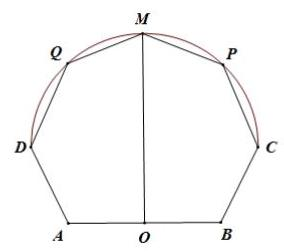
\includegraphics[max width=0.2\textwidth]{images/bo_d5jma53ef24c73bll4ig_124_1163_415_284_252_0.jpg}
\end{center}
\hspace*{3em} 

【例题】4. (2022 上海秋考) 如图,在同一平面上, \({AD} = {BC} = 6,{AB} = {20},O\) 为 \({AB}\) 中点,曲线 \({CD}\) 上任一点到 \(O\) 距离相等,角 \(\angle {DAB} = \angle {ABC} = \; {120}^{ \circ  },P\text{ 、 }Q\) 关于 \({OM}\) 对称, \({MO} \bot  {AB}\) ;

(1)若点 \(P\) 与点 \(C\) 重合，求 \(\angle {POB}\) 的大小；

(2) \(P\) 在何位置，求五边形 \({MQABP}\) 面积 \(S\) 的最大值.

【解析】(1)若 \(P\) 在点 \(C\) 的位置,则 \({OB} = {10},{BC} = {20},\angle {ABC} = {120}^{ \circ  }\) ,

在 \({OB} = {10},{BC} = {20},\angle {ABC} = {120}^{ \circ  },{\Delta OPB}\) 中,由余弦定理得

\(\cos \angle {OBC} = \frac{O{B}^{2} + B{C}^{2} - O{C}^{2}}{2 \times  {OB} \times  {BC}} =  - \frac{1}{2},\)

所以 \(\frac{{10}^{2} + {6}^{2} - O{C}^{2}}{2 \times  {10} \times  6} =  - \frac{1}{2} \Rightarrow  {OC} = {14}\) ,

在 \(\bigtriangleup {OPB}\) 中,由正弦定理得 \(\frac{OC}{\sin \angle {OBC}} = \frac{BC}{\sin \angle {POB}}\) ,

即 \(\frac{10}{\sin \angle {POB}} = \frac{14}{\sin {120}^{ \circ  }}\) ,所以 \(\sin \angle {POB} = \frac{3\sqrt{3}}{14}\) ,

因为 \(\angle {POB}\) 为锐角,所以 \(\angle {POB} = \arcsin \frac{3\sqrt{3}}{14}\) ;

(2) 连接 \({OQ},{OP}\) ,曲线 \({CMD}\) 上所有的点到 \(O\) 的距离相等,

\({OQ} = {OP} = {OD} = {OM} = {14}\) ,

\begin{center}
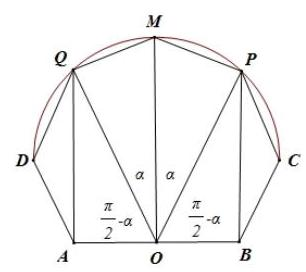
\includegraphics[max width=0.2\textwidth]{images/bo_d5jma53ef24c73bll4ig_124_1139_1132_306_272_0.jpg}
\end{center}
\hspace*{3em} 

点 \(Q\) 与点 \(P\) 关于 \({OM}\) 对称, \({S}_{\Delta QOM} = {S}_{\Delta POM},{S}_{\Delta AOM} = {S}_{\Delta BOM}\) ,

设 \(\angle {QOM} = \angle {POM} = \alpha ,\angle {QOA} = \angle {POB} = \frac{\pi }{2} - \alpha\) ,

则 \({S}_{\bigtriangleup {MQABP}} = 2\left( {{S}_{\bigtriangleup {MQO}} + {S}_{\bigtriangleup {QOA}}}\right)\)

\(= 2 \times  \left\lbrack  {\frac{1}{2}{OM} \times  {OQ} \times  \sin \alpha  + \frac{1}{2}{OA} \times  {OQ} \times  \sin \left( {\frac{\pi }{2} - \alpha }\right) }\right\rbrack\)

\(= {196}\sin \alpha  + {140}\cos \alpha  = {28}\sqrt{74}\sin \left( {\alpha  + \varphi }\right)\) ,其中 \(= {196}\sin \alpha  +\)

\({140}\cos \alpha  = \sqrt{58016}\sin \left( {\alpha  + \varphi }\right) ,\tan \varphi  = \frac{35}{64}.\)

所以当 \(\alpha  + \varphi  = \frac{\pi }{2}\) 时， \({\left( {S}_{{\Delta M}{QABP}}\right) }_{\max } = {{28}\sqrt{74}}\) ，

所以五边形 \({MQABP}\) 面积的最大值为 \({\left( {S}_{\Delta MQABP}\right) }_{\max } = {28}\sqrt{74}\) .

【例题】5. (2013 上海秋考) 已知函数 \(f\left( x\right)  = 2\sin \left( {\omega x}\right)\) ，其中常数 \(\omega  > 0\) .

(1) 若 \(y = f\left( x\right)\) 在 \(\left\lbrack  {-\frac{\pi }{4},\frac{2\pi }{3}}\right\rbrack\) 上单调递增，求 \(\omega\) 的取值范围；

(2) 令 \(\omega  = 2\) ,将函数 \(y = f\left( x\right)\) 的图象向左平移 \(\frac{\pi }{6}\) 个单位,再向上平移 1 个单位,得到函数 \(y = \; g\left( x\right)\) 的图象,区间 \(\left\lbrack  {a,b}\right\rbrack  \left( {a,b \in  R\text{ 且 }a < b}\right)\) 满足: \(y = g\left( x\right)\) 在 \(\left\lbrack  {a,b}\right\rbrack\) 上至少含有 30 个零点,在所有满足上述条件的 \(\left\lbrack  {a,b}\right\rbrack\) 中,求 \(b - a\) 的最小值.

【解析】(1) 因为 \(\omega  > 0,y = f\left( x\right)  = 2\sin {\omega x}\) 在 \(\left\lbrack  {-\frac{\pi }{4},\frac{2\pi }{3}}\right\rbrack\) 上单调递增,

所以 \(\left\{  \begin{array}{l}  - \frac{\pi }{4}\omega  \geq   - \frac{\pi }{2} \\  \frac{2\pi }{3}\omega  \leq  \frac{\pi }{2} \end{array}\right.\) ,解得 \(0 < \omega  \leq  \frac{3}{4}\) .

所以 \(\omega\) 的取值范围为 \(\left( {0,\frac{3}{4}}\right\rbrack\) .

(2)令 \(\omega  = 2\) ，将函数 \(y = f\left( x\right)  = 2\sin {2x}\) 的图象向左平移 \(\frac{\pi }{6}\) 个单位长度，

得函数 \(y = 2\sin 2\left( {x + \frac{\pi }{6}}\right)  = 2\sin \left( {{2x} + \frac{\pi }{3}}\right)\) 的图象;

再向上平移 1 个单位长度,得到函数 \(y = g\left( x\right)  = 2\sin \left( {{2x} + \frac{\pi }{3}}\right)  + 1\) 的图象,

令 \(g\left( x\right)  = 0\) ,得 \(\sin \left( {{2x} + \frac{\pi }{3}}\right)  =  - \frac{1}{2}\) ,

所以 \({2x} + \frac{\pi }{3} = {2k\pi } + \frac{7\pi }{6}\) ,或 \({2x} + \frac{\pi }{3} = {2k\pi } + \frac{11\pi }{6},k \in  Z\) ,

得 \(x = {k\pi } + \frac{5\pi }{12}\) 或 \(x = {k\pi } + \frac{3\pi }{4},k \in  Z\) ,

故函数 \(g\left( x\right)\) 的零点为 \(x = {k\pi } + \frac{5\pi }{12}\) 或 \(x = {k\pi } + \frac{3\pi }{4},k \in  Z\)

所以相邻两个零点之间的距离为 \(\frac{\pi }{3}\) 或 \(\frac{2\pi }{3}\) .

若 \(b - a\) 最小,则 \(a\) 和 \(b\) 都是零点,

此时在区间 \(\left\lbrack  {a,\pi  + a}\right\rbrack  ,\left\lbrack  {a,{2\pi } + a}\right\rbrack  ,\cdots ,\left\lbrack  {a,{m\pi } + a}\right\rbrack  \left( {m \in  {N}^{ * }}\right)\) 分别

恰有 \(3,5,\cdots ,{2m} + 1\) 个零点,所以在区间 \(\left\lbrack  {a,{14\pi } + a}\right\rbrack\) 是恰有 29 个零点,

从而在区间 \(({14\pi } + a,b\rbrack\) 至少有一个零点,所以 \(b - a - {14\pi } \geq  \frac{\pi }{3}\) .

另一方面，在区间 \(\left\lbrack  {\frac{5\pi }{12},{14\pi } + \frac{\pi }{3} + \frac{5\pi }{12}}\right\rbrack\) 恰有 30 个零点，

因此 \(b - a\) 的最小值为 \({14\pi } + \frac{\pi }{3} = \frac{43\pi }{3}\) . 2025 版上海高考真题及模拟训练合集

\section*{2. 模拟练习}

【练习】1. (23 宝山一模) 已知函数 \(f\left( x\right)  = \sin {2x} + \sqrt{3}\cos {2x},x \in  R\) .

(1)求函数 \(f\left( x\right)\) 的单调增区间;

(2)在锐角 \({\Delta ABC}\) 中，角 \(A\) 、 \(B\) 、 \(C\) 的对边分别为 \(a\) 、 \(b\) 、 \(c\) ，当 \(f\left( A\right)  = 0\) ， \(b = 1\) ，且三角形 \({ABC}\) 的面积为 \(\sqrt{3}\) 时，求 \(a\) .

【答案】 \(\left( 1\right) x \in  \left\lbrack  {{k\pi } - \frac{5\pi }{12},{k\pi } + \frac{\pi }{12}}\right\rbrack  ,k \in  Z;\left( 2\right) \sqrt{13}\)

【解析】(1) 由题意得 \(f\left( x\right)  = 2\sin \left( {{2x} + \frac{\pi }{3}}\right) ,x \in  R\) 3 分

当 \({2x} + \frac{\pi }{3} \in  \left\lbrack  {{2k\pi } - \frac{\pi }{2},{2k\pi } + \frac{\pi }{2}}\right\rbrack\) 5 分

即 \(x \in  \left\lbrack  {{k\pi } - \frac{5\pi }{12},{k\pi } + \frac{\pi }{12}}\right\rbrack  ,k \in  Z\) 为单调增区间 6 分

(2) \(f\left( A\right)  = 2\sin \left( {{2A} + \frac{\pi }{3}}\right)  = 0\) ，且 \(A\) 为锐角，解得 \(A = \frac{\pi }{3}\) 8 分

又 \(b = 1\) ,由 \(S = \frac{1}{2}{bc}\sin A\) 得 \(\sqrt{3} = \frac{1}{2}c\sin \frac{\pi }{3}\) ,从而 \(c = 4\) 10 分

由余弦定理 \(\cos A = \frac{{b}^{2} + {c}^{2} - {a}^{2}}{2bc}\) 12 分

代入得 \(\frac{1 + {16} - {a}^{2}}{2 \times  1 \times  4} = \frac{1}{2}\) ，解得 \({a}^{2} = {13}\) ，所以 \(a = \sqrt{13}\) 14 分

【练习】2. (23 金山一模) 在 \(\bigtriangleup  {ABC}\) 中，设角 \(A\) 、 \(B\) 、 \(C\) 所对的边分别为 \(a\) 、 \(b\) 、 \(c\) ，且 \(a\cos B + \left( {b - {4c}}\right) \cos A \; = 0\) .

(1)求 \(\cos A\) ；

( 2 )若 \(\overrightarrow{BD} = 2\overrightarrow{DC},\left| \overrightarrow{AD}\right|  = 1\) ，求 \(c + {2b}\) 的最大值.

【答案】 \(\left( 1\right) \frac{1}{4};\left( 2\right) \frac{6\sqrt{10}}{5}\)

【解析】(1) 由 \(a\cos B + \left( {b - {4c}}\right) \cos A = 0\) ,

得 \(\sin A\cos B + \left( {\sin B - 4\sin C}\right) \cos A = 0\) , 1 分

即 \(\sin \left( {A + B}\right)  - 4\sin C\cos A = 0\) , 4 分

从而 \(\sin C - 4\sin C\cos A = 0\) ,

由 \(\sin C > 0\) ,得 \(\cos A = \frac{1}{4}\) 6 分

(2) 由 \(\cos \angle {ADB} + \cos \angle {ADC} = 0\) 得 \(\frac{1 + \frac{4}{9}{a}^{2} - {c}^{2}}{2 \times  1 \times  \frac{2}{3}a} + \frac{1 + \frac{1}{9}{a}^{2} - {b}^{2}}{2 \times  1 \times  \frac{1}{3}a} = 0\) ，

从而 \(1 + \frac{4}{9}{a}^{2} - {c}^{2} + 2\left( {1 + \frac{1}{9}{a}^{2} - {b}^{2}}\right)  = 0\) ,即 \({a}^{2} = \frac{3}{2}\left( {{c}^{2} + 2{b}^{2} - 3}\right)\) 8 分

又因为 \(\cos A = \frac{1}{4} = \frac{{b}^{2} + {c}^{2} - {a}^{2}}{2bc}\) ,得 \({a}^{2} = {b}^{2} + {c}^{2} - \frac{1}{2}{bc}\) 9 分

所以 \({b}^{2} + {c}^{2} - \frac{1}{2}{bc} = \frac{3}{2}\left( {{c}^{2} + 2{b}^{2} - 3}\right)\) ,即 \({c}^{2} + {bc} + 4{b}^{2} = 9\) ,

从而 \({\left( c + 2b\right) }^{2} - 9 = {3bc}\) , 10 分

而 \({3bc} = \frac{3}{2}\left( {2b}\right)  \cdot  c \leq  \frac{3}{2} \cdot  \frac{{\left( 2b + c\right) }^{2}}{4}\) ,故 \({\left( c + 2b\right) }^{2} - 9 \leq  \frac{3{\left( 2b + c\right) }^{2}}{8}\) 12 分

解得 \({\left( c + 2b\right) }^{2} \leq  \frac{72}{5}\) ,当且仅当 \(b = \frac{3\sqrt{10}}{10},c = \frac{3\sqrt{10}}{5}\) 时取等号,

所以 \(c + {2b}\) 的最大值为 \(\frac{6\sqrt{10}}{5}\) 14 分

2025 版上海高考真题及模拟训练合集

【练习】3. (23 宝山二模) 已知函数 \(f\left( x\right)  = \sin x\cos x - \sqrt{3}{\cos }^{2}x + \frac{\sqrt{3}}{2}\) .

(1)求函数 \(y = f\left( x\right)\) 的最小正周期和单调区间；

(2)若关于 \(x\) 的方程 \(f\left( x\right)  - m = 0\) 在 \(x \in  \left\lbrack  {0,\frac{\pi }{2}}\right\rbrack\) 上有两个不同的实数解,求实数 \(m\) 的取值范围.

【解析】(1) \(f\left( x\right)  = \sin x\cos x - \sqrt{3}{\cos }^{2}x + \frac{\sqrt{3}}{2} = \frac{1}{2}\sin {2x} - \sqrt{3} \cdot  \frac{1 + \cos {2x}}{2} + \frac{\sqrt{3}}{2}\)

\(= \frac{1}{2}\sin {2x} - \frac{\sqrt{3}}{2}\cos {2x} = \sin \left( {{2x} - \frac{\pi }{3}}\right)\)

最小正周期 \(T = \pi \cdots \cdots 4\) 分

当 \({2x} - \frac{\pi }{3} \in  \left\lbrack  {{2k\pi } - \frac{\pi }{2},{2k\pi } + \frac{\pi }{2}}\right\rbrack\) ,即 \(x \in  \left\lbrack  {{k\pi } - \frac{\pi }{12},{k\pi } + \frac{5\pi }{12}}\right\rbrack  \left( {k \in  Z}\right)\) 时,函数为增函数.

6 分

当 \({2x} - \frac{\pi }{3} \in  \left\lbrack  {{2k\pi } + \frac{\pi }{2},{2k\pi } + \frac{3\pi }{2}}\right\rbrack\) ,即 \(x \in  \left\lbrack  {{k\pi } + \frac{5\pi }{12},{k\pi } + \frac{11\pi }{12}}\right\rbrack  \left( {k \in  Z}\right)\) 时,函数为减函数. \(\cdots \; \cdots 8\) 分

( 2 )方程 \(f\left( x\right)  - m = 0\) 有两个不同的实数解，

等价于 \(y = \sin \left( {{2x} - \frac{\pi }{3}}\right)\) 和直线 \(y = m\) 的图像在 \(x \in  \left\lbrack  {0,\frac{\pi }{2}}\right\rbrack\) 上有两个不同的交点. 10 分 \(x \in  \left\lbrack  {0,\frac{\pi }{2}}\right\rbrack\) ,则 \({2x} - \frac{\pi }{3} \in  \left\lbrack  {-\frac{\pi }{3},\frac{2\pi }{3}}\right\rbrack  ,\sin \left( {{2x} - \frac{\pi }{3}}\right)  \in  \left\lbrack  {-\frac{\sqrt{3}}{2},1}\right\rbrack  , \cdot\) 12 分

由图像得 \(m \in  \left\lbrack  {\frac{\sqrt{3}}{2},1}\right)\) .

\section*{板块四:压轴主观题}

\section*{1. 真题回顾}

【例题】1. (2019 上海春考) 已知等差数列 \(\left\{  {a}_{n}\right\}\) 的公差 \(d \in  (0,\pi \rbrack\) ,数列 \(\left\{  {b}_{n}\right\}\) 满足 \({b}_{n} = \sin \left( {a}_{n}\right)\) ,集合 \(S = \; \left\{  {x \mid  x = {b}_{n},n \in  {N}^{ * }}\right\}  .\)

(1)若 \({a}_{1} = 0,d = \frac{2\pi }{3}\) ，求集合 \(S\) ；

( 2 )若 \({a}_{1} = \frac{\pi }{2}\) ，求 \(d\) 使得集合 \(S\) 恰好有两个元素；

(3)若集合 \(S\) 恰好有三个元素: \({b}_{n + T} = {b}_{n}\) ， \(T\) 是不超过 7 的正整数，求 \(T\) 的所有可能的值.

【解析】(1) 因为等差数列 \(\left\{  {a}_{n}\right\}\) 的公差 \(d \in  (0,\pi \rbrack\) ,数列 \(\left\{  {b}_{n}\right\}\) 满足 \({b}_{n} = \sin \left( {a}_{n}\right)\) ,

集合 \(S = \left\{  {x \mid  x = {b}_{n},n \in  {N}^{ * }}\right\}\) . 所以当 \({a}_{1} = 0,d = \frac{2\pi }{3}\) ，集合 \(S = \left\{  {-\frac{\sqrt{3}}{2},0,\frac{\sqrt{3}}{2}}\right\}\) .

(2)因为 \({a}_{1} = \frac{\pi }{2}\) ，数列 \(\left\{  {b}_{n}\right\}\) 满足 \({b}_{n} = \sin \left( {a}_{n}\right)\) ，

\begin{center}
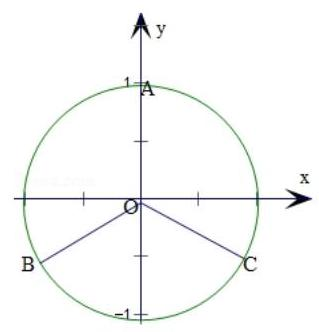
\includegraphics[max width=0.2\textwidth]{images/bo_d5jma53ef24c73bll4ig_128_1138_772_319_332_0.jpg}
\end{center}
\hspace*{3em} 

集合 \(S = \left\{  {x \mid  x = {b}_{n},n \in  {N}^{ * }}\right\}\) 恰好有两个元素，如图:

根据三角函数线， \circled{1} 等差数列 \(\left\{  {a}_{n}\right\}\) 的终边落在 \(y\) 轴的正负半轴上时,

集合 \(S\) 恰好有两个元素,此时 \(d = \pi\) ,

 \circled{2}  \({a}_{1}\) 终边落在 \({OA}\) 上，要使得集合 \(S\) 恰好有两个元素，可以使 \({a}_{2}\) ， \({a}_{3}\) 的终边关

于 \(y\) 轴对称,如图 \({OB},{OC}\) ,此时 \(d = \frac{2\pi }{3}\) ,

\begin{center}
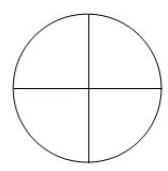
\includegraphics[max width=0.2\textwidth]{images/bo_d5jma53ef24c73bll4ig_128_1286_1155_168_171_0.jpg}
\end{center}
\hspace*{3em} 

综上, \(d = \frac{2}{3}\pi\) 或 \(d = \pi\) .

(3)  \circled{1}  当 \(T = 3\) 时， \({b}_{n + 3} = {b}_{n}\) ，集合 \(S = \left\{  {{b}_{1},{b}_{2},{b}_{3}}\right\}\) ，符合题意.

 \circled{2}  当 \(T = 4\) 时， \({b}_{n + 4} = {b}_{n}\) ， \(\sin \left( {{a}_{n} + {4d}}\right)  = \sin {a}_{n}\) ， \({a}_{n} + {4d} = {a}_{n} + {2k\pi }\) ，

或 \({a}_{n} + {4d} = \left( {{2k} + 1}\right) \pi  - {a}_{n}\) ,

等差数列 \(\left\{  {a}_{n}\right\}\) 的公差 \(d \in  (0,\pi \rbrack\) ,故 \({a}_{n} + {4d} = {a}_{n} + {2k\pi },d = \frac{k\pi }{2}\) ,

所以 \(k = 1,2\) ,当 \(k = 1\) 时满足条件,此时 \(S = \{ 0,1, - 1\}\) .

 \circled{3}  当 \(T = 5\) 时， \({b}_{n + 5} = {b}_{n}\) ， \(\sin \left( {{a}_{n} + {5d}}\right)  = \sin {a}_{n}\) ， \({a}_{n} + {5d} = {a}_{n} + {2k\pi }\) ，

\begin{center}
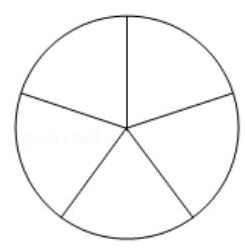
\includegraphics[max width=0.2\textwidth]{images/bo_d5jma53ef24c73bll4ig_128_1207_1471_245_248_0.jpg}
\end{center}
\hspace*{3em} 

或 \({a}_{n} + {5d} = \left( {{2k} + 1}\right) \pi  - {a}_{n}\) ,因为 \(d \in  (0,\pi \rbrack\) ,所以 \(k = 1,2\) .

当 \(k = 1\) 时， \(S = \left\{  {\sin \frac{2\pi }{5},1, - \sin \frac{2\pi }{5}}\right\}\) 满足题意.

 \circled{4}  当 \(T = 6\) 时， \({b}_{n + 6} = {b}_{n}\) ， \(\sin \left( {{a}_{n} + {6d}}\right)  = \sin {a}_{n}\) ，

所以 \({a}_{n} + {6d} = {a}_{n} + {2k\pi }\) 或 \({a}_{n} + {6d} = \left( {{2k} + 1}\right) \pi  - {a}_{n},d \in  (0,\pi \rbrack\) ,

故 \(k = 1,2,3\) . 当 \(k = 1\) 时, \(S = \left\{  {\frac{\sqrt{3}}{2},0,\frac{\sqrt{3}}{2}}\right\}\) ,满足题意.

 \circled{5}  当 \(T = 7\) 时， \({b}_{n + 7} = {b}_{n}\) ， \(\sin \left( {{a}_{n} + {7d}}\right)  = \sin {a}_{n} = \sin {a}_{n}\) ，

\begin{center}
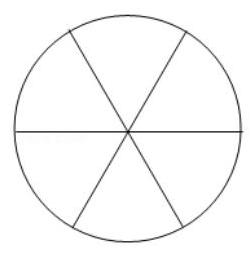
\includegraphics[max width=0.2\textwidth]{images/bo_d5jma53ef24c73bll4ig_128_1207_1793_250_253_0.jpg}
\end{center}
\hspace*{3em} 

所以 \({a}_{n} + {7d} = {a}_{n} + {2k\pi }\) 或 \({a}_{n} + {7d} = \left( {{2k} + 1}\right) \pi  - {a}_{n},d \in  (0,\pi \rbrack\) ,

故 \(k = 1,2,3\) ,当 \(k = 1\) 时,因为 \({b}_{1} \sim  {b}_{7}\) 对应着 3 个正弦值,

所以必有一个正弦值对应着 3 个点,必然有 \({a}_{m} - {a}_{n} = {2\pi },d = \frac{2\pi }{m - n} = \; \frac{2\pi }{7}\) ,

\(m - n = 7,m > 7\) ,不符合条件.

当 \(k = 2\) 时，因为 \({b}_{1} \sim  {b}_{7}\) 对应着 3 个正弦值，故必有一个正弦值对应着 3 个点，

必然有 \({a}_{m} - {a}_{n} = {2\pi },d = \frac{2\pi }{m - n} = \frac{4\pi }{7},m - n\) 不是整数，不符合条件.

当 \(k = 3\) 时，因为 \({b}_{1} \sim  {b}_{7}\) 对应着 3 个正弦值，故必有一个正弦值对应着 3 个点，

必然有 \({a}_{m} - {a}_{n} = {2\pi }\) 或 \({4\pi },d = \frac{2\pi }{m - n} = \frac{6\pi }{7}\) 或 \(d = \frac{4\pi }{m - n} = \frac{6\pi }{7}\) ,

此时, \(m - n\) 均不是整数,不符合题意.

综上, \(T = 3,4,5,6\) .

【例题】2. (2009 上海春考) 设函数 \({f}_{n}\left( \theta \right)  = {\sin }^{n}\theta  + {\left( -1\right) }^{n}{\cos }^{n}\theta ,0 \leq  \theta  \leq  \frac{\pi }{4}\) ,其中 \(n\) 为正整数.

(1)判断函数 \({f}_{1}\left( \theta \right)\) 、 \({f}_{3}\left( \theta \right)\) 的单调性,并就 \({f}_{1}\left( \theta \right)\) 的情形证明你的结论;

(2) 证明: \(2{f}_{6}\left( \theta \right)  - {f}_{4}\left( \theta \right)  = \left( {{\cos }^{4}\theta  - {\sin }^{4}\theta }\right) \left( {{\cos }^{2}\theta  - {\sin }^{2}\theta }\right)\) ;

(3)对于任意给定的正奇数 \(n\) ，求函数 \({f}_{n}\left( \theta \right)\) 的最大值和最小值.

【解析】 \(\left( 1\right) {f}_{1}\left( \theta \right) \text{ 、 }{f}_{3}\left( \theta \right)\) 在 \(0 \leq  \theta  \leq  \frac{\pi }{4}\) 上均为单调递增的函数.

对于函数 \({f}_{1}\left( \theta \right)  = \sin \theta  - \cos \theta\) ,设 \({\theta }_{1} < {\theta }_{2},{\theta }_{1}\text{ 、 }{\theta }_{2} \in  \left\lbrack  {0,\frac{\pi }{4}}\right\rbrack\) ,

则 \({f}_{1}\left( {\theta }_{1}\right)  - {f}_{1}\left( {\theta }_{2}\right)  = \left( {\sin {\theta }_{1} - \sin {\theta }_{2}}\right)  + \left( {\cos {\theta }_{2} - \cos {\theta }_{1}}\right)\) ,

因为 \(\sin {\theta }_{1} < \sin {\theta }_{2},\cos {\theta }_{2} < \cos {\theta }_{1}\) ,所以 \({f}_{1}\left( {\theta }_{1}\right)  < {f}_{1}\left( {\theta }_{2}\right)\) ,

所以函数 \({f}_{1}\left( \theta \right)\) 在 \(\left\lbrack  {0,\frac{\pi }{4}}\right\rbrack\) 上单调递增.

(2) 因为原式左边 \(= 2\left( {{\sin }^{6}\theta  + {\cos }^{6}\theta }\right)  - \left( {{\sin }^{4}\theta  + {\cos }^{4}\theta }\right)\)

\(= 2\left( {{\sin }^{2}\theta  + {\cos }^{2}\theta }\right) \left( {{\sin }^{4}\theta  - {\sin }^{2}\theta {\cos }^{2}\theta  + {\cos }^{4}\theta }\right)  - \left( {{\sin }^{4}\theta  + {\cos }^{4}\theta }\right)\)

\(= 1 - {\sin }^{2}{2\theta } = {\cos }^{2}{2\theta }\) .

又因为原式右边 \(= \left( {{\cos }^{2}\theta  - {\sin }^{2}\theta }\right) 2 = {\cos }^{2}{2\theta }\) ,

所以 \(2{f}_{6}\left( \theta \right)  - {f}_{4}\left( \theta \right)  = \left( {{\cos }^{4}\theta  - {\sin }^{4}\theta }\right) \left( {{\cos }^{2}\theta  - {\sin }^{2}\theta }\right)\) .

(3)当 \(n = 1\) 时，函数 \({f}_{1}\left( \theta \right)\) 在 \(\left\lbrack  {0,\frac{\pi }{4}}\right\rbrack\) 上单调递增，

所以 \({f}_{1}\left( \theta \right)\) 的最大值为 \({f}_{1}\left( \frac{\pi }{4}\right)  = 0\) ,最小值为 \({f}_{1}\left( 0\right)  =  - 1\) .

当 \(n = 3\) 时,函数 \({f}_{3}\left( \theta \right)\) 在 \(\left\lbrack  {0,\frac{\pi }{4}}\right\rbrack\) 上单调递增.

所以 \({f}_{3}\left( \theta \right)\) 的最大值为 \({f}_{3}\left( \frac{\pi }{4}\right)  = 0\) ,最小值为 \({f}_{3}\left( 0\right)  =  - 1\) .

下面讨论正奇数 \(n \geq  5\) 的情形: 对任意 \({\theta }_{1},{\theta }_{2} \in  \left\lbrack  {0,\frac{\pi }{4}}\right\rbrack\) ,且 \({\theta }_{1} < {\theta }_{2}\) ,

因为 \({f}_{n}\left( {\theta }_{1}\right)  - {f}_{n}\left( {\theta }_{2}\right)  = \left( {{\sin }^{n}{\theta }_{1} - {\sin }^{n}{\theta }_{2}}\right)  + \left( {{\cos }^{n}{\theta }_{2} - {\cos }^{n}{\theta }_{1}}\right)\) ,

以及 \(0 \leq  \sin {\theta }_{1} < \sin {\theta }_{2} < 1,0 \leq  \cos {\theta }_{2} < \cos {\theta }_{1} < 1\) ,

所以 \({\sin }^{n}{\theta }_{1} < {\sin }^{n}{\theta }_{2}{\cos }^{n}{\theta }_{2} < {\cos }^{n}{\theta }_{1}\) ,从而 \({f}_{n}\left( {\theta }_{1}\right)  < {f}_{n}\left( {\theta }_{2}\right)\) .

所以 \({f}_{n}\left( \theta \right)\) 在 \(\left\lbrack  {0,\frac{\pi }{4}}\right\rbrack\) 上为单调递增,

则 \({f}_{n}\left( \theta \right)\) 的最大值为 \({f}_{n}\left( \frac{\pi }{4}\right)  = 0\) ,最小值为 \({f}_{n}\left( 0\right)  =  - 1\) .

综上所述,当 \(n\) 为奇数时,函数 \({f}_{n}\left( \theta \right)\) 的最大值为 0,最小值为 -1 . 2025 版上海高考真题及模拟训练合集

\section*{2. 模拟练习}

【练习】1. 已知 \(\left\{  {a}_{n}\right\}\) 是等差数列, \({b}_{n} = \sin \left( {a}_{n}\right)\) ,且存在正整数 \(t\) ,使得对任意的正整数 \(n\) 都有 \({b}_{n + t} = {b}_{n}\) . 若集合 \(S = \left\{  {x \mid  x = {b}_{n},n\text{ 为正整数 }}\right\}\) 中只含有 4 个元素,则 \(t\) 的取值不可能是 ( )

A. 4 B. 5 C. 6 D. 7

【答案】 \(B\)

【解析】设等差数列 \(\left\{  {a}_{n}\right\}\) 首项为 \({a}_{1}\) ,公差为 \(d\) ,则 \({a}_{n} = {a}_{1} + \left( {n - 1}\right) d,{b}_{n} = \sin \left( {a}_{n}\right)\) ,

由题意得存在正整数 \(t\) ,使得 \({b}_{n + t} = {b}_{n},n \in  {N}^{ * }\) ,

若集合 \(\left\{  {x \mid  x = {b}_{n},n \in  {N}^{ * }}\right\}\) 有 4 个不同元素,得 \(t \geq  4\) ,

当 \(t = 4\) 时, \(\sin \left( {a}_{n + 4}\right)  = \sin \left( {a}_{n}\right)\) ,即 \(\sin \left( {a}_{n + 4}\right)  = \sin \left( {{a}_{n} + {4d}}\right)  = \sin \left( {{a}_{n} + {2k\pi }}\right) ,k \in  Z\) ,

所以 \({a}_{n + 4} = {a}_{n} + {4d} = {a}_{n} + {2k\pi }\) 或 \({a}_{n} + {4d} = \pi  - {a}_{n} + {2k\pi }\) (舍去), \(k \in  Z\) ,

所以 \(d = \frac{2k\pi }{4} = \frac{k\pi }{2},k \in  Z\) ,取 \(k = 1\) 时, \(d = \frac{\pi }{2}\) ,

在单位圆上的 4 个等分点可取到 4 个不同的正弦值,

即集合 \(\left\{  {x \mid  x = {b}_{n},n \in  {N}^{ * }}\right\}\) 可取 4 个不同元素;

当 \(k = 5,\sin \left( {a}_{n + 5}\right)  = \sin \left( {a}_{n}\right)\) ,即 \(\sin \left( {a}_{n + 5}\right)  = \sin \left( {{a}_{n} + {5d}}\right)  = \sin \left( {{a}_{n} + {2k\pi }}\right) ,k \in  Z\) ,

所以 \(d = \frac{2k\pi }{5}\) ,此时在单位圆上的 5 个等分点,

取到的 \(\sin \frac{2\pi }{5}\text{ 、 }\sin \frac{4\pi }{5}\text{ 、 }\sin \frac{6\pi }{5}\text{ 、 }\sin \frac{8\pi }{5}\text{ 、 }\sin \frac{10\pi }{5}\) ,

不可能取到 4 个不同的正弦值, 故不成立;

同理,当 \(t = 6,t = 7,t = 8\) ,集合 \(\left\{  {x \mid  x = {b}_{n},n \in  {N}^{ * }}\right\}\) 可取 4 个不同元素;

当 \(t \geq  9\) 时, \(d = \frac{2k\pi }{9}\) ,单位圆上至少 9 个等分点取 4 个不同的正弦值,

必有至少 3 个相等的正弦值,不符合集合 \(\left\{  {x \mid  x = {b}_{n},n \in  {N}^{ * }}\right\}\) 元素的互异性,故选 \(B\) .

【练习】2. (23 嘉定二模 21) 已知 \(f\left( x\right)  = x + 2\sin x\) ,等差数列 \(\left\{  {a}_{n}\right\}\) 的前 \(n\) 项和为 \({S}_{n}\) ,记 \({T}_{n} = \mathop{\sum }\limits_{{i = 1}}^{n}f\left( {a}_{i}\right)\) .

(1)求证:函数 \(y = f\left( x\right)\) 的图像关于点 \(\left( {\pi ,\pi }\right)\) 中心对称；

(2)若 \({a}_{1}\) 、 \({a}_{2}\) 、 \({a}_{3}\) 是某三角形的三个内角，求 \({T}_{3}\) 的取值范围；

(3) 若 \({S}_{100} = {100\pi }\) ，求证: \({T}_{100} = {100\pi }\) . 反之是否成立？并请说明理由.

【解析】(1) 在函数 \(y = x + 2\sin x\) 的图像上任取一点 \(P\left( {x,y}\right)\) ,

点 \(P\) 关于点 \(\left( {\pi ,\pi }\right)\) 的对称点为 \({P}^{\prime }\left( {{2\pi } - x,{2\pi } - y}\right)\) ,

而 \(f\left( {{2\pi } - x}\right)  = {2\pi } - x + 2\sin \left( {{2\pi } - x}\right)  = {2\pi } - x - 2\sin x = {2\pi } - y\) ,

所以点 \({P}^{\prime }\left( {{2\pi } - x,{2\pi } - y}\right)\) 在函数 \(y = f\left( x\right)\) 图像上,

所以函数 \(y = f\left( x\right)\) 的图像关于点 \(\left( {\pi ,\pi }\right)\) 中心对称.

(2)若 \({a}_{1}\text{ 、 }{a}_{2}\text{ 、 }{a}_{3}\) 是某三角形的三个内角,则 \({a}_{1} + {a}_{2} + {a}_{3} = \pi\) ，

又 \(\left\{  {a}_{n}\right\}\) 为等差数列,则 \({a}_{2} = \frac{\pi }{3}\) ,

\({T}_{3} = f\left( {a}_{1}\right)  + f\left( {a}_{2}\right)  + f\left( {a}_{3}\right)  = {a}_{1} + {a}_{2} + {a}_{3} + 2\left( {\sin {a}_{1} + \sin {a}_{2} + \sin {a}_{3}}\right)\)

\(= \pi  + \sqrt{3} + 2\left( {\sin {a}_{1} + \sin {a}_{3}}\right)\) ,

\({T}_{3} = \pi  + \sqrt{3} + 4\left( {\sin \frac{{a}_{1} + {a}_{3}}{2}\cos \frac{{a}_{1} - {a}_{3}}{2}}\right)  = \pi  + \sqrt{3} + 2\sqrt{3}\cos \frac{{a}_{1} - {a}_{3}}{2},\)

不妨设 \(0 < {a}_{1} \leq  {a}_{3} < \frac{2}{3}\pi\) ,则 \(- \frac{2}{3}\pi  < {a}_{1} - {a}_{3} \leq  0\) ,于是 \(\cos \frac{{a}_{1} - {a}_{3}}{2} \in  \left( {\frac{1}{2},1}\right\rbrack\) ,

所以 \({T}_{3} \in  (\pi  + 2\sqrt{3},\pi  + 3\sqrt{3}\rbrack\) ;

(3) 若 \({S}_{100} = {100\pi }\) ,又 \({T}_{100} = \mathop{\sum }\limits_{{i = 1}}^{{100}}f\left( {a}_{i}\right)  = {S}_{100} + 2\mathop{\sum }\limits_{{i = 1}}^{{100}}\sin {a}_{i}\) ,

则 \({T}_{100} = {100\pi } + 2\mathop{\sum }\limits_{{i = 1}}^{{100}}\sin {a}_{i}\) ,

因为 \(\left\{  {a}_{n}\right\}\) 为等差数列且 \({S}_{100} = {100\pi }\) ,所以当 \(n + m = {101}\) 时, \({a}_{n} + {a}_{m} = {2\pi }\) ,

于是 \(\sin {a}_{n} + \sin {a}_{m} = 0\) .

故 \(2\mathop{\sum }\limits_{{i = 1}}^{{100}}\sin {a}_{i} = \left( {\sin {a}_{1} + \sin {a}_{100}}\right)  + \left( {\sin {a}_{2} + \sin {a}_{99}}\right)  + \cdots  + \left( {\sin {a}_{100} + \sin {a}_{1}}\right)  = 0\) ,

所以 \({T}_{100} = {100\pi }\) ,得证.

若 \({T}_{100} = {100\pi }\) ,则 \({S}_{100} + 2\mathop{\sum }\limits_{{i = 1}}^{{100}}\sin {a}_{i} = {100\pi }\) ,反之不成立.

考虑存在等差数列 \(\left\{  {a}_{n}\right\}\) ,满足 \({a}_{50} = {a}_{1} + {49d} = \pi\) ,则 \({S}_{99} = {99\pi }\) ,

于是 \({a}_{n}\) 与 \({a}_{{100} - n}\) 关于 \(\pi\) 对称,所以 \({T}_{99} = {99\pi }\) .

下面证明，存在 \(d\) 可以使得 \(f\left( {a}_{100}\right)  = \pi\) 且 \({a}_{100} \neq  \pi\) .

不妨设 \(d > 0\) ,又 \({a}_{1} + {49d} = \pi\) ,所以 \({a}_{100} = {a}_{1} + {99d} \neq  \pi\) .

\(f\left( {a}_{100}\right)  - \pi  = {50d} - 2\sin \left( {50d}\right)\) ,考虑函数 \(y = x - 2\sin x,x > 0\) ,

其中 \(g\left( x\right)  = x - 2\sin x\) ,

因为 \(g\left( \frac{\pi }{3}\right)  = \frac{\pi }{3} - \sqrt{3} < 0,g\left( \pi \right)  = \pi  > 0\) ,所以存在 \(\xi  \in  \left( {\frac{\pi }{3},\pi }\right)\) 使得 \(g\left( \xi \right)  = 0\) ,

所以存在 \(d \in  \left( {\frac{\pi }{150},\frac{\pi }{50}}\right)\) ,使得 \(f\left( {a}_{100}\right)  = \pi\) 即 \({T}_{100} = {100\pi }\) ,

但是 \({S}_{100} \neq  {100\pi }\) . 所以反之不成立.

注: 反例不唯一,例如: 考虑 \(d = 0\) ,证明存在 \(\xi  \in  \left( {\frac{3\pi }{2},{2\pi }}\right)\) ,使得 \(f\left( \xi \right)  = \pi ,{a}_{n} = \xi\) .

\section*{五、平面向量与复数}

板块一:中档客观题

\section*{1. 真题回顾}

A、复数常见性质

【例题】1. (2024 上海秋考) 设 \(m \in  R\) ，已知虚数 \(z\) 的实部为 1 且满足 \(z + \frac{2}{z} = m\) ，则 \(m\) 的值为\_\_\_\_\_.

【答案】 2

【解析】设 \(z = 1 + {bi},b \in  R,b \neq  0\) ,则 \(z + \frac{2}{z} = 1 + {bi} + \frac{2}{1 + {bi}} = 1 + {bi} + \frac{2\left( {1 - {bi}}\right) }{1 + {b}^{2}}\)

\(= \left( {1 + \frac{2}{1 + {b}^{2}}}\right)  + \left( {b - \frac{2b}{1 + {b}^{2}}}\right) \mathrm{i} = m \in  R\) ,所以 \(b - \frac{2b}{1 + {b}^{2}} = 0\) ,

因为 \(b \neq  0\) ，所以 \(1 - \frac{2}{1 + {b}^{2}} = 0\) ，则 \({b}^{2} = 1\) ，所以 \(m = \left( {1 + \frac{2}{1 + {b}^{2}}}\right)  = 2\) .

【例题】2. (2018 上海春考) 设 \(m \in  R\) ，若 \(z\) 是关于 \(x\) 的方程 \({x}^{2} + {mx} + {m}^{2} - 1 = 0\) 的一个虚根，则 \(\left| \bar{z}\right|\) 的取值范围是\_\_\_\_\_.

【答案】 \(\left( {\frac{\sqrt{3}}{3}, + \infty }\right)\)

【解析】设 \(z = a + {bi}\left( {a,b \in  R}\right)\) ,则 \(\bar{z} = a - {bi}\) 也为此方程的一个虚根.

\(z\) 是关于 \(x\) 的方程 \({x}^{2} + {mx} + {m}^{2} - 1 = 0\) 的一个虚根,得 \({m}^{2} - 4\left( {{m}^{2} - 1}\right)  < 0,{m}^{2} > \frac{4}{3}\)

所以 \({a}^{2} + {b}^{2} = {m}^{2} - 1\) ,则 \(\left| \bar{z}\right|  = \sqrt{{m}^{2} - 1} > \frac{\sqrt{3}}{3}\) ,则 \(\left| \bar{z}\right|\) 的取值范围是 \(\left( {\frac{\sqrt{3}}{3}, + \infty }\right)\) .

【例题】3. (2015 上海春考) 关于 \(x\) 的实系数一元二次方程 \({x}^{2} + {px} + 2 = 0\) 的两个虚数根为 \({z}_{1}\text{ 、 }{z}_{2}\) ，若 \({z}_{1}\text{ 、 }{z}_{2}\) 在复平面上对应的点是经过原点的椭圆的两个焦点，则该椭圆的长轴长为\_\_\_\_\_.

【答案】 \(2\sqrt{2}\)

【解析】因为 \(p\) 为实数, \(p \neq  0,{z}_{1},{z}_{2}\) 为虚数,所以 \({p}^{2} - 4 \times  2 < 0\) ,即 \({p}^{2} < 8\) ,

解得 \(- 2\sqrt{2} < p < 2\sqrt{2}\) ,由 \({z}_{1},{z}_{2}\) 为共轭复数,得 \({Z}_{1},{Z}_{2}\) 关于 \(x\) 轴对称,

所以椭圆短轴在 \(x\) 轴上,又由椭圆经过原点,得原点为椭圆短轴的一端点,

由椭圆的性质,复数加、减法几何意义及一元二次方程根与系数的关系,

得椭圆的短轴长 \(= {2b} = \left| {{z}_{1} + {z}_{2}}\right|  = \left| p\right|\) ,焦距 \({2c} = \left| {{z}_{1} - {z}_{2}}\right|  = \sqrt{8 - {p}^{2}}\) ,

长轴长 \({2a} = \sqrt{8 - {p}^{2} + {p}^{2}} = 2\sqrt{2}\) .

【例题】4. (2014 上海秋考) 已知互异的复数 \(a,b\) 满足 \({ab} \neq  0\) ，集合 \(\left\{  {a,b}\right\}   = \left\{  {{a}^{2},{b}^{2}}\right\}\) ，则 \(a + b =\) \_\_\_\_\_.

【答案】 -1

【解析】由集合相等的条件得若 \(\{ a,b\}  = \left\{  {{a}^{2},{b}^{2}}\right\}\) ,则 \(\left\{  \begin{array}{l} a = {a}^{2} \\  b = {b}^{2} \end{array}\right.\)  \circled{1} 或 \(\left\{  \begin{array}{l} a = {b}^{2} \\  b = {a}^{2} \end{array}\right.\)  \circled{2} ，

由 \circled{1} 得 \(\left\{  \begin{array}{l} a = 0\text{ 或 }a = 1 \\  b = 0\text{ 或 }b = 1 \end{array}\right.\) ，因为 \({ab} \neq  0\) ，所以 \(a \neq  0\) 且 \(b \neq  0\) ，即 \(a = 1,b = 1\) ，

此时集合 \(\{ 1,1\}\) 不满足条件.

若 \(b = {a}^{2},a = {b}^{2}\) ,则两式相减得 \({a}^{2} - {b}^{2} = b - a\) ,因为互异的复数 \(a,b\) ,

所以 \(b - a \neq  0\) ,即 \(a + b =  - 1\) . 2025 版上海高考真题及模拟训练合集

\section*{B、平面向量建系运算}

【例题】1. (2022 上海秋考) 已知 \(\lambda  > 0,\left| \overrightarrow{a}\right|  = \left| \overrightarrow{b}\right|  = \left| \overrightarrow{c}\right|  = \lambda\) ,且 \(\overrightarrow{a} \cdot  \overrightarrow{b} = 0,\overrightarrow{c} \cdot  \overrightarrow{a} = 2,\overrightarrow{c} \cdot  \overrightarrow{b} = 1\) ,则 \(\lambda  =\) \_\_\_\_\_.

【答案】 \({5}^{\frac{1}{4}}\)

【解析】法一:建立平面直角坐标系,设 \(\overrightarrow{a} = \left( {\lambda ,0}\right) ,\overrightarrow{b} = \left( {0,\lambda }\right) ,\overrightarrow{c} = \left( {x,y}\right)\) ,

由 \(\overrightarrow{a} \cdot  \overrightarrow{b} = 0,\overrightarrow{c} \cdot  \overrightarrow{a} = 2,\overrightarrow{c} \cdot  \overrightarrow{b} = 1\) 得 \(\left\{  \begin{array}{l} {\lambda x} = 2 \\  {\lambda y} = 1 \\  \sqrt{{x}^{2} + {y}^{2}} = \lambda  \end{array}\right.\) ,又 \(\lambda  > 0\) ,解得 \(\lambda  = {5}^{\frac{1}{4}}\) .

法二: 记 \(< \overrightarrow{a},\overrightarrow{c} >  = \theta\) ,由 \(\overrightarrow{a} \cdot  \overrightarrow{b} = 0,\overrightarrow{a} \cdot  \overrightarrow{c} = 2,\overrightarrow{b} \cdot  \overrightarrow{c} = 1\) ,首先 \(0 < \theta  < \frac{\pi }{2}\) ,

进而 \(\frac{\overrightarrow{a} \cdot  \overrightarrow{c}}{\overrightarrow{b} \cdot  \overrightarrow{c}} = \frac{\cos \theta }{\cos \left( {\frac{\pi }{2} - \theta }\right) } = \frac{1}{\tan \theta } = 2\) ,故 \(\cos \theta  = \frac{2\sqrt{5}}{5}\) ,

代入 \(\overrightarrow{a} \cdot  \overrightarrow{c} = 2\) 得 \(\lambda  = {5}^{\frac{1}{4}}\) .

法三:同上，由题意得 \({\lambda }^{2}\cos \theta  = 2\)  \circled{1} ， \({\lambda }^{2}\cos \left( {\frac{\pi }{2} - \theta }\right)  = 1\) ，

即 \({\lambda }^{2}\sin \theta  = 1\)  \circled{2} ，将两式分别平方，之后再相加，得 \({\lambda }^{4} = 5\) ，即 \(\lambda  = {5}^{\frac{1}{4}}\) .

【例题】2. (2022 上海春考) 在 \(\bigtriangleup {ABC}\) 中， \(\angle C = \frac{\pi }{2}\) ，且 \({AC} = {BC} = 2\) ， \(M\) 为边 \({AC}\) 的中点. 若 \(P\) 在边 \({AB}\) 上运动 (点 \(P\) 可与 \(A,B\) 重合),则 \(\overrightarrow{MP} \cdot  \overrightarrow{CP}\) 的最小值为\_\_\_\_\_.

【答案】 \(\frac{7}{8}\)

\begin{center}
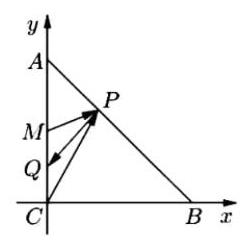
\includegraphics[max width=0.2\textwidth]{images/bo_d5jma53ef24c73bll4ig_133_1207_1180_242_242_0.jpg}
\end{center}
\hspace*{3em} 

【解析】法一: 建系,设 \(P\left( {x,2 - x}\right)\) ,

则 \(\overrightarrow{MP} \cdot  \overrightarrow{CP} = \left( {x,1 - x}\right)  \cdot  \left( {x,2 - x}\right)  = 2{x}^{2} - {3x} + 2\)

\(= 2{\left( x - \frac{3}{4}\right) }^{2} + \frac{7}{8} \geq  \frac{7}{8},\)

故 \(\overrightarrow{MP} \cdot  \overrightarrow{CP}\) 的最小值为 \(\frac{7}{8}\) .

法二:极化恒等式， \(\overrightarrow{MP} \cdot  \overrightarrow{CP} = \overrightarrow{PM} \cdot  \overrightarrow{PC} = {\overrightarrow{PQ}}^{2} - {\overrightarrow{QC}}^{2}\)

\(= {\overrightarrow{PQ}}^{2} - \frac{1}{4} \geq  {\left( \frac{3}{2\sqrt{2}}\right) }^{2} - \frac{1}{4} = \frac{7}{8}\) ,故 \(\overrightarrow{MP} \cdot  \overrightarrow{CP}\) 的最小值为 \(\frac{7}{8}\) .

【例题】3. (2020 上海春考) 已知 \({A}_{1}\text{ 、 }{A}_{2}\text{ 、 }{A}_{3}\text{ 、 }{A}_{4}\text{ 、 }{A}_{5}\) 五个点,满足 \(\overrightarrow{{A}_{n}{A}_{n + 1}} \cdot  \overrightarrow{{A}_{n + 1}{A}_{n + 2}} = 0\left( {n = 1,2,3}\right)\) , \(\left| \overrightarrow{{A}_{n}{A}_{n + 1}}\right|  \cdot  \left| \overrightarrow{{A}_{n + 1}{A}_{n + 2}}\right|  = n + 1\left( {n = 1,2,3}\right)\) ，则 \(\left| \overrightarrow{{A}_{1}{A}_{5}}\right|\) 的最小值为\_\_\_\_\_.

【答案】 \(\frac{\sqrt{6}}{3}\)

\begin{center}
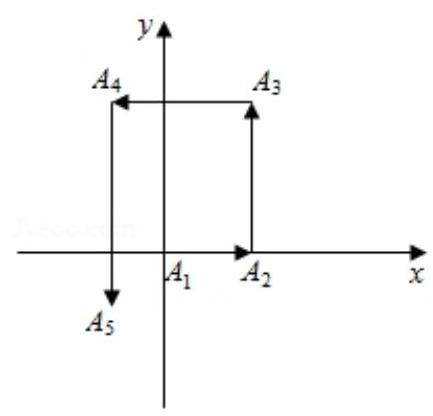
\includegraphics[max width=0.3\textwidth]{images/bo_d5jma53ef24c73bll4ig_133_1017_1689_433_416_0.jpg}
\end{center}
\hspace*{3em} 

【解析】设 \(\left| \overrightarrow{{A}_{1}{A}_{2}}\right|  = x\) ,则 \(\left| \overrightarrow{{A}_{2}{A}_{3}}\right|  = \frac{2}{x},\left| \overrightarrow{{A}_{3}{A}_{4}}\right|  = \frac{3x}{2},\left| \overrightarrow{{A}_{4}{A}_{5}}\right|  = \frac{8}{3x}\) , 设 \({A}_{1}\left( {0,0}\right)\) ,如图,

因为求 \(\left| \overrightarrow{{A}_{1}{A}_{5}}\right|\) 的最小值,

则 \({A}_{2}\left( {x,0}\right) ,{A}_{3}\left( {x,\frac{2}{x}}\right) ,{A}_{4}\left( {-\frac{x}{2},\frac{2}{x}}\right) ,{A}_{5}\left( {-\frac{x}{2}, - \frac{2}{3x}}\right)\) ,

所以 \({\left| \overrightarrow{{A}_{1}{A}_{5}}\right| }^{2} = {\left( -\frac{x}{2}\right) }^{2} + {\left( -\frac{2}{3x}\right) }^{2} = \frac{{x}^{2}}{4} + \frac{4}{9{x}^{2}} \geq  \frac{2}{3}\) ,

当且仅当 \(\frac{{x}^{2}}{4} = \frac{4}{9{x}^{2}}\) ,即 \(x = \frac{2\sqrt{3}}{3}\) 时取等号,

所以 \(\left| \overrightarrow{{A}_{1}{A}_{5}}\right|\) 的最小值为 \(\frac{\sqrt{6}}{3}\) .

【例题】4. (2018 上海秋考) 在平面直角坐标系中,已知点 \(A\left( {-1,0}\right) \text{ 、 }B\left( {2,0}\right) ,E\text{ 、 }F\) 是 \(y\) 轴上的两个动点，且 \(\left| \overrightarrow{EF}\right|  = 2\) ，则 \(\overrightarrow{AE} \cdot  \overrightarrow{BF}\) 的最小值为\_\_\_\_\_.

【答案】 -3

【解析】设 \(E\left( {0,a}\right) ,F\left( {0,b}\right)\) ,所以 \(\left| \overrightarrow{EF}\right|  = \left| {a - b}\right|  = 2\) ,所以 \(a = b + 2\) 或 \(b = a + 2\) ,

且 \(\overrightarrow{AE} = \left( {1,a}\right) ,\overrightarrow{BF} = \left( {-2,b}\right)\) ,所以 \(\overrightarrow{AE} \cdot  \overrightarrow{BF} =  - 2 + {ab}\) ;

当 \(a = b + 2\) 时, \(\overrightarrow{AE} \cdot  \overrightarrow{BF} =  - 2 + \left( {b + 2}\right) b = {b}^{2} + {2b} - 2\) ,

因为 \({b}^{2} + {2b} - 2\) 的最小值为 \(\frac{-8 - 4}{4} =  - 3\) ，所以 \(\overrightarrow{AE} \cdot  \overrightarrow{BF}\) 的最小值为 -3,

同理可得 \(b = a + 2\) 时, \(\overrightarrow{AE} \cdot  \overrightarrow{BF}\) 的最小值为 -3,

所以 \(\overrightarrow{AE} \cdot  \overrightarrow{BF}\) 的最小值为 -3 .

【例题】5. (2016 上海秋考) 在平面直角坐标系中,已知 \(A\left( {1,0}\right) ,B\left( {0, - 1}\right) ,P\) 是曲线 \(y = \sqrt{1 - {x}^{2}}\) 上一个动点,则 \(\overrightarrow{BP} \cdot  \overrightarrow{BA}\) 的取值范围是\_\_\_\_\_.

【答案】 \(\left\lbrack  {0,1 + \sqrt{2}}\right\rbrack\)

【解析】在平面直角坐标系中, \(A\left( {1,0}\right) ,B\left( {0, - 1}\right) ,P\) 是曲线 \(y = \sqrt{1 - {x}^{2}}\) 上一个动点,

设 \(P\left( {\cos \alpha ,\sin \alpha }\right) ,\alpha  \in  \left\lbrack  {0,\pi }\right\rbrack\) ,所以 \(\overrightarrow{BA} = \left( {1,1}\right) ,\overrightarrow{BP} = \left( {\cos \alpha ,\sin \alpha  + 1}\right)\) ,

\(\overrightarrow{BP} \cdot  \overrightarrow{BA} = \cos \alpha  + \sin \alpha  + 1 = \sqrt{2}\sin \left( {\alpha  + \frac{\pi }{4}}\right)  + 1,\)

所以 \(\overrightarrow{BP} \cdot  \overrightarrow{BA}\) 的取值范围是 \(\left\lbrack  {0,1 + \sqrt{2}}\right\rbrack\) .

【例题】6. (2012上海秋考)在平行四边形 \({ABCD}\) 中， \(\angle A = \frac{\pi }{3}\) ，边 \({AB}\) 、 \({AD}\) 的长分别为2、1，若 \(M\) 、 \(N\) 分别是边 \({BC}\) 、 \({CD}\) 上的点,且满足 \(\frac{\left| \overrightarrow{BM}\right| }{\left| \overrightarrow{BC}\right| } = \frac{\left| \overrightarrow{CN}\right| }{\left| \overrightarrow{CD}\right| }\) ,则 \(\overrightarrow{AM} \cdot  \overrightarrow{AN}\) 的取值范围是\_\_\_\_\_.

【答案】 \(\left\lbrack  {2,5}\right\rbrack\)

\begin{center}
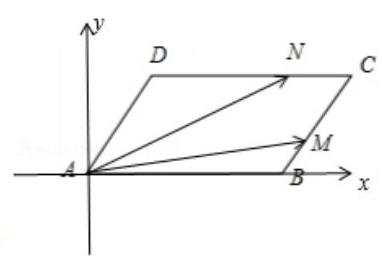
\includegraphics[max width=0.3\textwidth]{images/bo_d5jma53ef24c73bll4ig_134_1075_1358_382_264_0.jpg}
\end{center}
\hspace*{3em} 

【解析】建立如图所示的直角坐标系,则 \(B\left( {2,0}\right) ,A\left( {0,0}\right)\) ,

\(D\left( {\frac{1}{2},\frac{\sqrt{3}}{2}}\right)\) ,设 \(\frac{\left| \overrightarrow{BM}\right| }{\left| \overrightarrow{BC}\right| } = \frac{\left| \overrightarrow{CN}\right| }{\left| \overrightarrow{CD}\right| } = \lambda ,\lambda  \in  \left\lbrack  {0,1}\right\rbrack\) ,

\(M\left( {2 + \frac{\lambda }{2},\frac{\sqrt{3}\lambda }{2}}\right) ,N\left( {\frac{5}{2} - {2\lambda },\frac{\sqrt{3}}{2}}\right) ,\)

所以 \(\overrightarrow{AM} \cdot  \overrightarrow{AN} = \left( {2 + \frac{\lambda }{2},\frac{\sqrt{3}\lambda }{2}}\right)  \cdot  \left( {\frac{5}{2} - {2\lambda },\frac{\sqrt{3}}{2}}\right)  =  - {\lambda }^{2} - {2\lambda } + 5\) ,

因为 \(\lambda  \in  \left\lbrack  {0,1}\right\rbrack\) ,二次函数的对称轴为 \(\lambda  =  - 1\) ,

所以 \(\lambda  \in  \left\lbrack  {0,1}\right\rbrack\) 时, \(- {\lambda }^{2} - {2\lambda } + 5 \in  \left\lbrack  {2,5}\right\rbrack\) ,

所以 \(\overrightarrow{AM} \cdot  \overrightarrow{AN}\) 的取值范围是 \(\left\lbrack  {2,5}\right\rbrack\) . 2025 版上海高考真题及模拟训练合集

\section*{C、平面向量分解}

【例题】1. (2021 上海春考) 在 \(\bigtriangleup {ABC}\) 中， \(D\) 为 \({BC}\) 中点， \(E\) 为 \({AD}\) 中点，则以下结论:

 \circled{1}  存在 \(\bigtriangleup {ABC}\) ，使得 \(\overrightarrow{AB} \cdot  \overrightarrow{CE} = 0\) ；

 \circled{2} 存在 \(\bigtriangleup {ABC}\) ，使得 \(\overrightarrow{CE}//\left( {\overrightarrow{CB} + \overrightarrow{CA}}\right)\) ；

它们的成立情况是 ( )

A.  \circled{1} 成立， \circled{2} 成立 B.  \circled{1} 成立， \circled{2} 不成立

C.  \circled{1} 不成立， \circled{2} 成立 D.  \circled{1} 不成立， \circled{2} 不成立

【答案】 \(B\)

\begin{center}
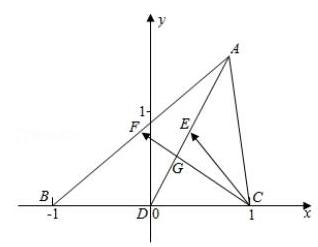
\includegraphics[max width=0.2\textwidth]{images/bo_d5jma53ef24c73bll4ig_135_1138_642_318_247_0.jpg}
\end{center}
\hspace*{3em} 

【解析】不妨设 \(A\left( {{2x},{2y}}\right) ,B\left( {-1,0}\right) ,C\left( {1,0}\right) ,D\left( {0,0}\right) ,E\left( {x,y}\right)\) ,

 \circled{1}  \(\overrightarrow{AB} = \left( {-1 - {2x}, - {2y}}\right) ,\overrightarrow{CE} = \left( {x - 1,y}\right)\) ，

若 \(\overrightarrow{AB} \cdot  \overrightarrow{CE} = 0\) ,则 \(- \left( {1 + {2x}}\right) \left( {x - 1}\right)  - 2{y}^{2} = 0\) ,

即 \(- \left( {1 + {2x}}\right) \left( {x - 1}\right)  = 2{y}^{2}\) ,

满足条件的 \(\left( {x,y}\right)\) 存在,例如 \(\left( {0,\frac{\sqrt{2}}{2}}\right)\) ,满足上式,所以 \circled{1} 成立; \({AD}\)  \circled{2}  \(F\) 为 \({AB}\) 中点， \(\left( {\overrightarrow{CB} + \overrightarrow{CA}}\right)  = 2\overrightarrow{CF}\) ， \({CF}\) 与 \({AD}\) 的交点即为重心 \(G\) ，

因为 \(G\) 为 \({AD}\) 的三等分点， \(E\) 为中点，所以 \(\overrightarrow{CE}\) 与 \(\overrightarrow{CG}\) 不共线，即 \circled{2} 不成立.

故选 \(B\) .

\begin{center}
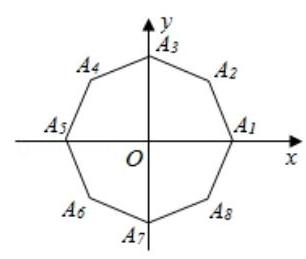
\includegraphics[max width=0.2\textwidth]{images/bo_d5jma53ef24c73bll4ig_135_1148_1055_306_259_0.jpg}
\end{center}
\hspace*{3em} 

【例题】2. (2016 上海秋考) 如图,在平面直角坐标系 \({xOy}\) 中, \(O\) 为正八边形 \({A}_{1}{A}_{2}\cdots {A}_{8}\) 的中心, \({A}_{1}\left( {1,0}\right)\) ,任取不同的两点 \({A}_{i}\text{ 、 }{A}_{j}\) ,点 \(P\) 满足 \(\overrightarrow{OP} + \; \overrightarrow{O{A}_{i}} + \overrightarrow{O{A}_{j}} = \overrightarrow{0}\) ，则点 \(P\) 落在第一象限的概率是\_\_\_\_\_.

【答案】 \(\frac{5}{28}\)

【解析】从正八边形 \({A}_{1}{A}_{2}\cdots {A}_{8}\) 的八个顶点中任取两个,基本事件总数为 \({C}_{8}^{2} \; = {28}\) .

满足 \(\overrightarrow{OP} + \overrightarrow{O{A}_{i}} + \overrightarrow{O{A}_{j}} = \overrightarrow{0}\) ，且点 \(P\) 落在第一象限，对应的 \({A}_{i}\) 、 \({A}_{j}\) ，

为 \(\left( {{A}_{4},{A}_{7}}\right) ,\left( {{A}_{5},{A}_{8}}\right) ,\left( {{A}_{5},{A}_{6}}\right) ,\left( {{A}_{6},{A}_{7}}\right) ,\left( {{A}_{5},{A}_{7}}\right)\) 共 5 种取法.

所以点 \(P\) 落在第一象限的概率是 \(P = \frac{5}{28}\) .

【例题】3. (2011 上海春考) 若 \(\overrightarrow{{a}_{1}}\text{ 、 }\overrightarrow{{a}_{2}}\text{ 、 }\overrightarrow{{a}_{3}}\) 均为单位向量,则 \(\overrightarrow{{a}_{1}} = \left( {\frac{\sqrt{3}}{3},\frac{\sqrt{6}}{3}}\right)\) 是 \(\overrightarrow{{a}_{1}} + \overrightarrow{{a}_{2}} + \overrightarrow{{a}_{3}} = \left( {\sqrt{3},\sqrt{6}}\right)\) 的 ( )

A. 充分不必要条件 B. 必要不充分条件

C. 充要条件 D. 既不充分也不必要条件

【答案】 \(B\)

【解析】 \({\overrightarrow{a}}_{1},{\overrightarrow{a}}_{2},{\overrightarrow{a}}_{3}\) 均为单位向量, \({\overrightarrow{a}}_{1} = \left( {\frac{\sqrt{3}}{3},\frac{\sqrt{6}}{3}}\right)\) ,若 \({\overrightarrow{a}}_{2} = \left( {\frac{\sqrt{3}}{3},\frac{\sqrt{6}}{3}}\right) ,{\overrightarrow{a}}_{3} = \left( {\frac{1}{2},\frac{\sqrt{3}}{2}}\right)\) ,

则 \({\overrightarrow{a}}_{1} + {\overrightarrow{a}}_{2} + {\overrightarrow{a}}_{3} = \left( {\sqrt{3},\sqrt{6}}\right)\) 不成立;

若 \({\overrightarrow{a}}_{1},{\overrightarrow{a}}_{2},{\overrightarrow{a}}_{3}\) 均为单位向量, \({\overrightarrow{a}}_{1} + {\overrightarrow{a}}_{2} + {\overrightarrow{a}}_{3} = \left( {\sqrt{3},\sqrt{6}}\right)\) ,则 \(\left| {{\overrightarrow{a}}_{1} + {\overrightarrow{a}}_{2} + {\overrightarrow{a}}_{3}}\right|  = 3\) ,

则 \({\overrightarrow{a}}_{1},{\overrightarrow{a}}_{2},{\overrightarrow{a}}_{3}\) 共线且同向,设 \({\overrightarrow{a}}_{1} = {\overrightarrow{a}}_{2} = {\overrightarrow{a}}_{3} = \left( {m,n}\right)\) ,易得 \(\left\{  \begin{array}{l} {3m} = \sqrt{3} \\  {3n} = \sqrt{6} \end{array}\right.\) ,

则 \({\overrightarrow{a}}_{1} = \left( {\frac{\sqrt{3}}{3},\frac{\sqrt{6}}{3}}\right)\) ,

所以 “ \({\overrightarrow{a}}_{1} = \left( {\frac{\sqrt{3}}{3},\frac{\sqrt{6}}{3}}\right)\) ” 是 “ \({\overrightarrow{a}}_{1} + {\overrightarrow{a}}_{2} + {\overrightarrow{a}}_{3} = \left( {\sqrt{3},\sqrt{6}}\right)\) ” 的必要不充分条件,

故选 \(B\) .

【例题】4. (2011 上海秋考) 设 \({A}_{1}\text{ 、 }{A}_{2}\text{ 、 }{A}_{3}\text{ 、 }{A}_{4},\text{ 、 }{A}_{5}\) 是平面上给定的 5 个不同点,则使 \(\overrightarrow{M{A}_{1}} + \overrightarrow{M{A}_{2}} + \overrightarrow{M{A}_{3}} + \overrightarrow{M{A}_{4}} + \overrightarrow{M{A}_{5}} = \overrightarrow{0}\) 成立的点 \(M\) 的个数为 ( )

A. 0 B. 1 C. 5 D. 10

【答案】 \(B\)

【解析】设 \(M\) 的坐标为 \(\left( {x,y}\right)\) ,再设 \({A}_{1}\text{ 、 }{A}_{2}\text{ 、 }{A}_{3}\text{ 、 }{A}_{4}\text{ 、 }{A}_{5}\) 的坐标依次为

\(\left( {{x}_{1},{y}_{1}}\right) \text{ 、 }\left( {{x}_{2},{y}_{2}}\right) \text{ 、 }\left( {{x}_{3},{y}_{3}}\right) \text{ 、 }\left( {{x}_{4},{y}_{4}}\right) \text{ 、 }\left( {{x}_{5},{y}_{5}}\right)\) ;

若 \(\overrightarrow{M{A}_{1}} + \overrightarrow{M{A}_{2}} + \overrightarrow{M{A}_{3}} + \overrightarrow{M{A}_{4}} + \overrightarrow{M{A}_{5}} = \overrightarrow{0}\) 成立，

得 \(\left( {{x}_{1} - x,{y}_{1} - y}\right)  + \left( {{x}_{2} - x,{y}_{2} - y}\right)  + \left( {{x}_{3} - x,{y}_{3} - y}\right)\)

\(+ \left( {{x}_{4} - x,{y}_{4} - y}\right)  + \left( {{x}_{5} - x,{y}_{5} - y}\right)  = \overrightarrow{0}\) ,

则 \(x = \frac{{x}_{1} + {x}_{2} + {x}_{3} + {x}_{4} + {x}_{5}}{5},y = \frac{{y}_{1} + {y}_{2} + {y}_{3} + {y}_{4} + {y}_{5}}{5}\) ;

只有一组解,即符合条件的点 \(M\) 有且只有一个; 故选 \(B\) . 2025 版上海高考真题及模拟训练合集

\section*{2. 模拟练习}

【练习】1. 设 \(\bigtriangleup {ABC},{P}_{0}\) 是边 \({AB}\) 上一定点,满足 \({P}_{0}B = \frac{1}{4}{AB}\) ,且对于边 \({AB}\) 上任一点 \(P\) ,恒有 \(\overrightarrow{PB} \cdot  \overrightarrow{PC} \; \geq  \overrightarrow{{P}_{0}B} \cdot  \overrightarrow{{P}_{0}C}\) . 则 ( )

\begin{center}
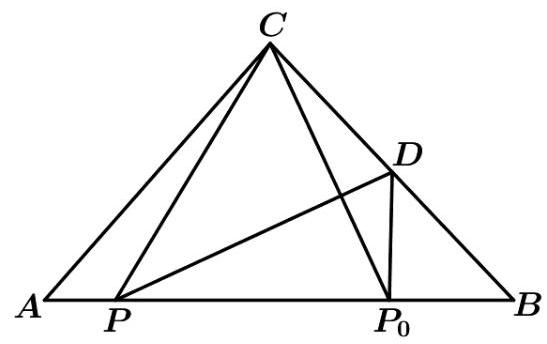
\includegraphics[max width=0.4\textwidth]{images/bo_d5jma53ef24c73bll4ig_137_296_401_547_344_0.jpg}
\end{center}
\hspace*{3em} 

A. \(\angle {ABC} = {90}^{ \circ  }\) B. \(\angle {BAC} = {90}^{ \circ  }\) C. \({AB} = {AC}\) D. \({AC} = {BC}\)

【答案】 \(D\)

【解析】如图,取 \({BC}\) 的中点 \(D\) ,

\begin{center}
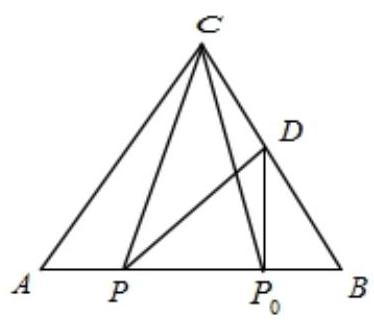
\includegraphics[max width=0.3\textwidth]{images/bo_d5jma53ef24c73bll4ig_137_1075_914_374_320_0.jpg}
\end{center}
\hspace*{3em} 

由极化恒等式可得: \(\overrightarrow{PB} \cdot  \overrightarrow{PC} = \overrightarrow{P{D}^{2}} - \overrightarrow{B{D}^{2}}\) ,

同理, \(\overrightarrow{{P}_{0}B} \cdot  \overrightarrow{{P}_{0}C} = \overrightarrow{{P}_{0}{D}^{2}} - \overrightarrow{B{D}^{2}}\) ,由于 \(\overrightarrow{PB} \cdot  \overrightarrow{PC} \geq  \overrightarrow{{P}_{0}B} \cdot  \overrightarrow{{P}_{0}C}\) ,

则 \(\left| \overrightarrow{PD}\right|  \geq  \left| \overrightarrow{{P}_{0}D}\right|\) ,所以 \({P}_{0}D \bot  {AB}\) ,

因为 \({P}_{0}B = \frac{1}{4}{AB},D\) 是 \({BC}\) 的中点,于是 \({AC} = {BC}\) .

故选: \(D\) .

【练习】2. 已知点 \({A}_{1},{A}_{2},\cdots ,{A}_{n}\left( {n \in  N,n \geq  2}\right)\) 均在圆 \(O\) 上,若有 \(\overrightarrow{O{A}_{1}} \; + \overrightarrow{O{A}_{2}} + \cdots  + \overrightarrow{O{A}_{n}} = \overrightarrow{0}\) ,则必有 \({A}_{1},{A}_{2},\cdots ,{A}_{n}\) 平分圆 \(O\) . 则满足要求的 \(n\) 的个数为 ( )

A. 0 个 B. 仅有 1 个 C. 仅有 2 个 D. 3 个或以上

【答案】C

【解析】由 \(\overrightarrow{O{A}_{1}} + \overrightarrow{O{A}_{2}} + \cdots  + \overrightarrow{O{A}_{n}} = \overrightarrow{0}\) ,

当 \(n = 2\) 时,两向量共线反向, \({A}_{1},{A}_{2}\) 平分圆 \(O\) ,符合题意,

当 \(n = 3\) ,由 \(\overrightarrow{O{A}_{1}} + \overrightarrow{O{A}_{2}} + \overrightarrow{O{A}_{3}} = \overrightarrow{0}\) ,设圆 \(O\) 的半径为 1,

变形可得 \(\overrightarrow{O{A}_{1}} =  - \overrightarrow{O{A}_{2}} - \overrightarrow{O{A}_{3}}\) ，两边平方可得 \({\overrightarrow{OA}}^{2} = {\overrightarrow{OA}}^{2} + 2\overrightarrow{O{A}_{2}} \cdot  \overrightarrow{O{A}_{3}} + {\overrightarrow{OA}}_{3}^{2}\) ，

所以 \(1 = 1 + 2 \times  1 \times  1 \times  \cos \angle {A}_{2}O{A}_{3} + 1\) ,解得 \(\cos \angle {A}_{2}O{A}_{3} =  - \frac{1}{2}\) ,

因为 \(0 < \angle {A}_{2}O{A}_{3} < \pi\) ,所以 \(\angle {A}_{2}O{A}_{3} = \frac{\pi }{3}\) ,同理可得 \(\angle {A}_{1}O{A}_{2} = \frac{\pi }{3},\angle {A}_{1}O{A}_{3} = \frac{\pi }{3}\) ,

所以 \({A}_{1},{A}_{2},{A}_{3}\) 平分圆 \(O\) ,

若 \(n \geq  4\) 时,

当 \(n\) 为偶数时,只要分为 \(\frac{n}{2}\) 对,每对共线,可得 \(\overrightarrow{O{A}_{1}} + \overrightarrow{O{A}_{2}} + \cdots  + \overrightarrow{O{A}_{n}} = \overrightarrow{0}\) ,

比如过圆心的两条直线与圆相交的四个点,满足 \(\overrightarrow{O{A}_{1}} + \overrightarrow{O{A}_{2}} + \cdots  + \overrightarrow{O{A}_{n}} = \overrightarrow{0}\) ,但不平分圆,

所认 \({A}_{1},{A}_{2},\cdots ,{A}_{8}\) 不一定平分圆,故不符合题意,

当 \(n\) 为奇数时,可分三个点,使这三个向量满足 \(\overrightarrow{O{A}_{1}} + \overrightarrow{O{A}_{2}} + \overrightarrow{O{A}_{3}} = \overrightarrow{0}\) ,

可得 \({A}_{1},{A}_{2},{A}_{3}\) 平分圆 \(O\) ,另外剩余的一定是偶数点,由前面知道,这些点可分组, 但不一定平分圆,故可得 \({A}_{1},{A}_{2},\cdots ,{A}_{8}\) 不一定平分圆, 综上所述，可得只有 \(n = 2\) 与 \(n = 3\) 符合题意，故选:C.

【练习】3. 已知平面向量 \(\overrightarrow{a},\overrightarrow{b},\overrightarrow{c},\overrightarrow{e}\) 满足 \(\left| \overrightarrow{a}\right|  = 4,\left| \overrightarrow{e}\right|  = 1,\left| {\overrightarrow{b} - \overrightarrow{a}}\right|  = 1,\langle \overrightarrow{a},\overrightarrow{e}\rangle  = \frac{2\pi }{3}\) ，且对任意的实数 \(t\) ，均有 \(\left| {\overrightarrow{c} - t\overrightarrow{e}}\right|  \geq  \left| {\overrightarrow{c} - 2\overrightarrow{e}}\right|\) ,则 \(\left| {\overrightarrow{c} - \overrightarrow{b}}\right|\) 的最小值为\_\_\_\_\_.

【解析】法一: 设 \(\overrightarrow{a} = \overrightarrow{OA} = \left( {4,0}\right) ,\overrightarrow{b} = \overrightarrow{OB} = \left( {x,y}\right) ,\overrightarrow{c} = \overrightarrow{OC},\overrightarrow{e} = \overrightarrow{OE}\) ,因为 \(\langle \overrightarrow{a},\overrightarrow{e}\rangle  = \frac{2\pi }{3}\) ,

所以设 \(E\left( {-\frac{1}{2},\frac{\sqrt{3}}{2}}\right)\) ，因为 \(\left| {\overrightarrow{b} - \overrightarrow{a}}\right|  = 1\) ，所以 \(B\) 在圆 \({\left( x - 4\right) }^{2} + {y}^{2} = 1\) 上运动，

设 \(t\overrightarrow{e} = \overrightarrow{OF},2\overrightarrow{e} = \overrightarrow{OG}\) ,则 \(\left| {\overrightarrow{c} - t\overrightarrow{e}}\right|  = {CF} \geq  \left| {\overrightarrow{c} - 2\overrightarrow{e}}\right|  = {CG}\) 恒成立,其中 \(G\left( {-1,\sqrt{3}}\right)\) ,

所以 \({CG} \bot  {OG}\) ,则 \(C\) 在直线 \(- \left( {x + 1}\right)  + \sqrt{3}\left( {y - \sqrt{3}}\right)  = 0\) ,即 \(x - \sqrt{3}y + 4 = 0\) 上,

则 \(\left| {\overrightarrow{c} - \overrightarrow{b}}\right|  = {BC}\) 的最小值即为圆心到直线的距离减去半径，即 \(\frac{4 + 4}{2} - 1 = 3\) .

法二: 令 \(\overrightarrow{OA} \equiv  \overrightarrow{a},\overrightarrow{OE} = \overrightarrow{e}\) ,以点 \(O\) 为原点, \(\overrightarrow{OA}\) 为 \(x\) 轴正方向建立直角坐标系,

因为 \(\left| \overrightarrow{a}\right|  = 4,\langle \overrightarrow{a},\overrightarrow{e}\rangle  = \frac{2\pi }{3},\left| \overrightarrow{e}\right|  = 1\) ,

所以点 \(A\) 的坐标为 \(\left( {4,0}\right)\) ，点 \(E\) 的坐标为 \(\left( {-\frac{1}{2},\frac{\sqrt{3}}{2}}\right)\) ，

\begin{center}
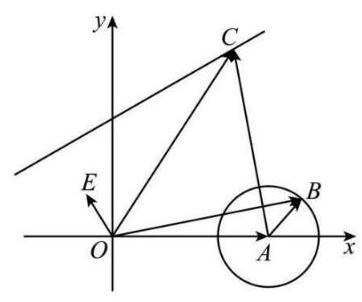
\includegraphics[max width=0.3\textwidth]{images/bo_d5jma53ef24c73bll4ig_138_1095_964_362_302_0.jpg}
\end{center}
\hspace*{3em} 

令 \(\overrightarrow{OB} = \overrightarrow{b}\) ,设点 \(B\) 的坐标为 \(\left( {x,y}\right)\) ,

因为 \(\left| \overrightarrow{AB}\right|  = \left| {\overrightarrow{OB} - \overrightarrow{OA}}\right|  = \left| {\overrightarrow{b} - \overrightarrow{a}}\right|  = 1\) ,

所以 \(\sqrt{{\left( x - 4\right) }^{2} + {y}^{2}} = 1\) ,所以 \({\left( x - 4\right) }^{2} + {y}^{2} = 1\) ,

所以点 \(B\) 在以 \(\left( {4,0}\right)\) 为圆心,以 1 为半径的圆上,

因为对任意的实数 \(t\) ,均有 \(\left| {\overrightarrow{c} - t\overrightarrow{e}}\right|  \geq  \left| {\overrightarrow{c} - 2\overrightarrow{e}}\right|\) ,

所以 \({\left| \overrightarrow{c} - t\overrightarrow{e}\right| }^{2} \geq  {\left| \overrightarrow{c} - 2\overrightarrow{e}\right| }^{2}\) ,又 \(\left| \overrightarrow{e}\right|  = 1\) ,所以 \({t}^{2} - 2\overrightarrow{e} \cdot  \overrightarrow{c}t + 4\overrightarrow{e} \cdot  \overrightarrow{c} - 4 \geq\) 0 恒成立,

所以 \({\left( 2\overrightarrow{e} \cdot  \overrightarrow{c}\right) }^{2} - 4\left( {4\overrightarrow{e} \cdot  \overrightarrow{c} - 4}\right)  \leq  0\) ,所以 \({\left( \overrightarrow{e} \cdot  \overrightarrow{c} - 2\right) }^{2} \leq  0\) ,即 \(\overrightarrow{e} \cdot  \overrightarrow{c} = 2\) ,

作 \(\overrightarrow{OC} = \overrightarrow{c}\) ,设点 \(C\) 的坐标为 \(\left( {{x}^{\prime },{y}^{\prime }}\right)\) ,则 \(- \frac{1}{2}{x}^{\prime } + \frac{\sqrt{3}}{2}{y}^{\prime } = 2\) ,即 \({x}^{\prime } - \sqrt{3}{y}^{\prime } + 4 = 0\) ,

以点 \(C\) 在直线 \({x}^{\prime } - \sqrt{3}{y}^{\prime } + 4 = 0\) 上,因为 \(\left| {\overrightarrow{c} - \overrightarrow{b}}\right|  = \left| {\overrightarrow{OC} - \overrightarrow{OB}}\right|  = \left| \overrightarrow{BC}\right|\) ,

又点 \(B\) 在圆 \({\left( x - 4\right) }^{2} + {y}^{2} = 1\) 上一动点,点 \(C\) 在直线 \({x}^{\prime } - \sqrt{3}{y}^{\prime } + 4 = 0\) 上一动点,

所以点 \(B\) 到点 \(C\) 的最小距离为点 \(A\) 到点 \(C\) 的距离减去圆的半径 1,

即 \(\left| \overrightarrow{BC}\right|  \geq  \left| \overrightarrow{AC}\right|  - 1\) ,当且仅当点 \(B\) 为线段 \({AC}\) 与圆的交点时取等号,

因为点 \(A\left( {4,0}\right)\) 到直线 \({x}^{\prime } - \sqrt{3}{y}^{\prime } + 4 = 0\) 的距离 \(d = \frac{8}{\sqrt{1 + 3}} = 4\) ,

所以点 \(A\) 到点 \(C\) 的距离大于等于 4,即 \(\left| \overrightarrow{AC}\right|  \geq  4\) ,所以 \(\left| \overrightarrow{BC}\right|  \geq  \left| \overrightarrow{AC}\right|  - 1 \geq  3\) ,

当且仅当 \({AC}\) 垂直于直线 \({x}^{\prime } - \sqrt{3}{y}^{\prime } + 4 = 0\) 且点 \(B\) 为 \({AC}\) 与圆的交点时取等号,

所以 \(\left| {\overrightarrow{c} - \overrightarrow{b}}\right|\) 的最小值为 3 .

【练习】4. 已知 \({Rt}{\Delta ABC}\) 中， \({\angle A} = {90}^{ \circ  },{AB} = 4,{AC} = 6\) ，在三角形所在的平面内有两个动点 \(M\) 和 \(N\) ， 满足 \(\left| \overrightarrow{AM}\right|  = 2,\overrightarrow{MN} = \overrightarrow{NC}\) ，则 \(\left| \overrightarrow{BN}\right|\) 的取值范围是\_\_\_\_\_.

【答案】 \(\left\lbrack  {4,6}\right\rbrack\)

【解析】如图示:

\begin{center}
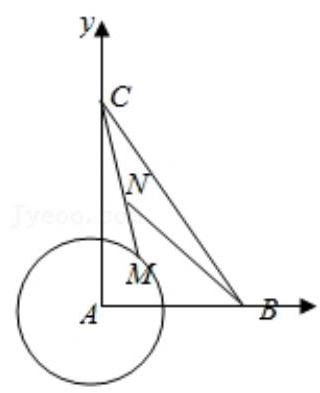
\includegraphics[max width=0.2\textwidth]{images/bo_d5jma53ef24c73bll4ig_139_1137_232_320_393_0.jpg}
\end{center}
\hspace*{3em} 

以 \({AB},{AC}\) 为坐标轴建立坐标系,则 \(B\left( {4,0}\right) ,C\left( {0,6}\right)\) ,

\(\because \left| \overrightarrow{AM}\right|  = 2,\therefore M\) 的轨迹是以 \(A\) 为圆心,以 2 为半径的圆,

\(\because \overrightarrow{MN} = \overrightarrow{NC},\therefore N\) 是 \({MC}\) 的中点,

设 \(M\left( {2\cos \alpha ,2\sin \alpha }\right)\) ,则 \(N\left( {\cos \alpha ,\sin \alpha  + 3}\right)\) ,

\(\therefore \overrightarrow{BN} = \left( {\cos \alpha  - 4,\sin \alpha  + 3}\right)\) ,

\(\therefore {\left| \overrightarrow{BN}\right| }^{2} = {\left( \cos \alpha  - 4\right) }^{2} + {\left( \sin \alpha  + 3\right) }^{2} = 6\sin \alpha  - 8\cos \alpha  + {26} = {10}\sin (\alpha \; - \varphi ) + {26}\) ,

\(\therefore\) 当 \(\sin \left( {\alpha  - \varphi }\right)  =  - 1\) 时, \(\left| \overrightarrow{BN}\right|\) 取得最小值 \(\sqrt{-{10} + {26}} = 4\) ,

当 \(\sin \left( {\alpha  - \varphi }\right)  = 1\) 时, \(\left| \overrightarrow{BN}\right|\) 取得最大值 \(\sqrt{{10} + {26}} = 6\) .

故答案为: \(\left\lbrack  {4,6}\right\rbrack\) .

【练习】5. \(\bigtriangleup  {ABC}\) 中， \({AB} = 3,{AC} = 6,G\) 为 \(\bigtriangleup  {ABC}\) 的重心， \(O\) 为 \(\bigtriangleup  {ABC}\) 的外心，则 \(\overrightarrow{AO} \cdot  \overrightarrow{AG} =\) \_\_\_\_\_. 【答案】 \(\frac{15}{2}\)

【解析】本题考查平面向量的数量积运算, 考查向量的线性运算法则, 是拔高题.

因为 \(G\) 为 \(\bigtriangleup {ABC}\) 的重心, \(O\) 为 \(\bigtriangleup {ABC}\) 的外心,得出 \(\overrightarrow{AO} \cdot  \overrightarrow{AB} = \frac{1}{2}\overrightarrow{AB}{}^{2},\overrightarrow{AO} \cdot  \overrightarrow{AC} = \frac{1}{2}\overrightarrow{AC}{}^{2}\) ,代入 \(\overrightarrow{AO} \cdot  \overrightarrow{AG} = \frac{1}{3}\overrightarrow{AO} \cdot  \left( {\overrightarrow{AB} + \overrightarrow{AC}}\right)  = \frac{1}{3}\overrightarrow{AO} \cdot  \overrightarrow{AB} + \frac{1}{3}\overrightarrow{AO} \cdot  \overrightarrow{AC}\) ,即可求解.

解: 因为 \(G\) 为 \(\bigtriangleup {ABC}\) 的重心, \(O\) 为 \(\bigtriangleup {ABC}\) 的外心,

所以 \(\overrightarrow{AO} \cdot  \overrightarrow{AB} = \frac{1}{2}\overrightarrow{AB}{}^{2},\overrightarrow{AO} \cdot  \overrightarrow{AC} = \frac{1}{2}\overrightarrow{AC}{}^{2}\) ,

所以 \(\overrightarrow{AO} \cdot  \overrightarrow{AG} = \frac{1}{3}\overrightarrow{AO} \cdot  \left( {\overrightarrow{AB} + \overrightarrow{AC}}\right)  = \frac{1}{3}\overrightarrow{AO} \cdot  \overrightarrow{AB} + \frac{1}{3}\overrightarrow{AO} \cdot  \overrightarrow{AC}\)

\(= \frac{1}{6}\overrightarrow{AB}{}^{2} + \frac{1}{6}\overrightarrow{AC}{}^{2} = \frac{9}{6} + \frac{36}{6} = \frac{15}{2}\) ,

即 \(\overrightarrow{AO} \cdot  \overrightarrow{AG} = \frac{15}{2}\) .

故答案为: \(\frac{15}{2}\) .

【练习】6. 如图所示,将一圆的八个等分点分成相间的两组,连接每组的四个点得到两个正方形. 去掉两个正方形内部的八条线段后可以形成一正八角星. 设正八角星的中心为 \(O\) ，并且 \(\overrightarrow{OA} = \; {\overrightarrow{\mathrm{e}}}_{1},\overrightarrow{OB} = {\overrightarrow{\mathrm{e}}}_{2}\) . 若将点 \(O\) 到正八角星 16 个顶点的向量都写成 \(\lambda {\overrightarrow{\mathrm{e}}}_{1} + \mu {\overrightarrow{\mathrm{e}}}_{2},\lambda ,\mu  \in  R\) 的形式,则 \(\lambda  + \; \mu\) 的取值范围为 ( )

\begin{center}
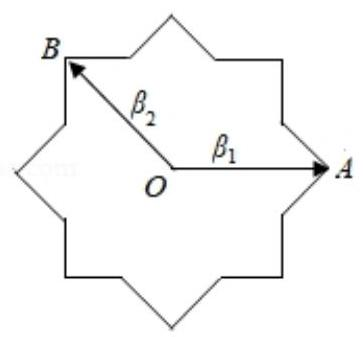
\includegraphics[max width=0.3\textwidth]{images/bo_d5jma53ef24c73bll4ig_139_351_1630_363_337_0.jpg}
\end{center}
\hspace*{3em} 

A. \(\left\lbrack  {-2\sqrt{2},2}\right\rbrack\) B. \(\left\lbrack  {-2\sqrt{2},1 + \sqrt{2}}\right\rbrack\)

C. \(\left\lbrack  {-1 - \sqrt{2},1 + \sqrt{2}}\right\rbrack\) D. \(\left\lbrack  {-1 - \sqrt{2},2}\right\rbrack\) 2025 版上海高考真题及模拟训练合集

【答案】 \(C\)

\begin{center}
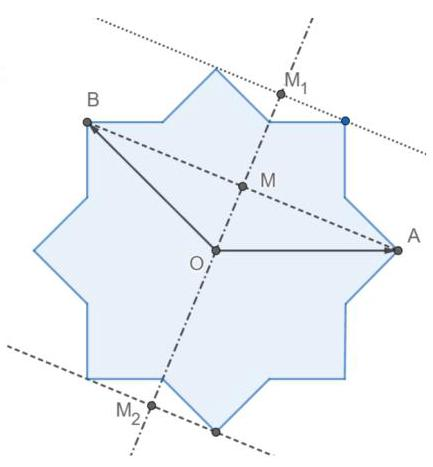
\includegraphics[max width=0.3\textwidth]{images/bo_d5jma53ef24c73bll4ig_140_1034_270_433_467_0.jpg}
\end{center}
\hspace*{3em} 

【解析】连线: 连接 \({AB}\) ,

平行:作 \({AB}\) 的平行线,与八角星顶点相交的平行线中,正方向最远和负方向最远分别如图所示,

求比值: 同一平行线上 \(\lambda  + \mu\) 的值相同,所以 \(\lambda  + \mu\) 最大是 \(\frac{\left| \overrightarrow{O{M}_{1}}\right| }{\left| \overrightarrow{OM}\right| }\) ，最小值是 \(- \frac{\left| \overrightarrow{O{M}_{2}}\right| }{\left| \overrightarrow{OM}\right| }\) ，几何法易得 \(\frac{\left| \overrightarrow{O{M}_{1}}\right| }{\left| \overrightarrow{OM}\right| } = \frac{\left| \overrightarrow{O{M}_{2}}\right| }{\left| \overrightarrow{OM}\right| } = \; 1 + \sqrt{2}\) ,故答案为 \(C\)

【练习】7. 设 \(\alpha\) 和 \(\beta\) 是关于 \(x\) 的方程 \({x}^{2} - {4x} + m = 0\) 的两个虚数根, 若 \(\alpha \text{ 、 }\beta \text{ 、 } - 1\) 在复平面上对应的点构成直角三角形,则实数 \(m =\) \_\_\_\_\_.

【答案】 13

【解析】设 \(\alpha  = a + {bi}\) ,则 \(\beta  = a - {bi}\) ,结合韦达定理可得 \(a = 2,m = {b}^{2} + 4\) ,根据题意可知 \({CA} \bot  {CB}\) ,结合向量的坐标运算求解.

设 \(\alpha  = a + {bi},a,b \in  R\) ,由实系数一元二次方程虚根成对定理可得 \(\beta  = \overline{\alpha } = a - {bi}\) ,

由根与系数的关系可得 \(\alpha  + \beta  = {2a} = 4,{\alpha \beta } = {a}^{2} + {b}^{2} = m\) ,

整理得 \(a = 2,m = {b}^{2} + 4\) ,

设 \(\alpha \text{ 、 }\beta \text{ 、 } - 1\) 在复平面上对应的点分别为 \(A\left( {2,b}\right) \text{ 、 }B\left( {2, - b}\right) \text{ 、 }C\left( {-1,0}\right)\) ,

则 \(\overrightarrow{CA} = \left( {3,b}\right) ,\overrightarrow{CB} = \left( {3, - b}\right)\) ,

可知 \(A,B\) 关于 \(x\) 轴对称,

若复平面上 \(\alpha\) 、 \(\beta\) 、 -1 对应点构成直角三角形，则 \({CA} \bot  {CB}\) ，

即 \(\overrightarrow{CA} \cdot  \overrightarrow{CB} = 9 - {b}^{2} = 0\) ,解得 \({b}^{2} = 9\) ,

所以 \(m = {b}^{2} + 4 = {13}\) .

故答案为:13 .

【练习】8. 在平面直角坐标系中,已知点 \(A\left( {2,0}\right) ,B\left( {0,2}\right)\) ,圆 \(C : {\left( x - a\right) }^{2} + {y}^{2} = 1\) ,

若圆 \(C\) 上存在点 \(M\) ，使得 \({\left| MA\right| }^{2} + {\left| MB\right| }^{2} = {12}\) ，则实数 \(a\) 的取值范围为\_\_\_\_\_

【答案】 \(\left\lbrack  {1 - 2\sqrt{2},1 + 2\sqrt{2}}\right\rbrack\)

【解析】先求出动点 \(M\) 的轨迹是圆 \(D\) ,再根据圆 \(D\) 和圆 \(C\) 相交或相切,得到 \(a\) 的取值范围. 设 \(M(x\) , \(y)\) ,则 \({\left( x - 2\right) }^{2} + {y}^{2} + {x}^{2} + {\left( y - 2\right) }^{2} = {12}\) ,

所以 \({\left( x - 1\right) }^{2} + {\left( y - 1\right) }^{2} = 4\) ,

所以点 \(M\) 的轨迹是一个圆 \(D\) ,

由题得圆 \(C\) 和圆 \(D\) 相交或相切,

所以 \(1 \leq  \sqrt{{\left( 1 - a\right) }^{2} + {1}^{2}} \leq  3\) ,

所以 \(1 - 2\sqrt{2} \leq  a \leq  1 + 2\sqrt{2}\) .

\section*{板块二: 压轴客观题}

\section*{1. 真题回顾}

A、与距离相关

【例题】1. (2023 上海春考) 设 \({z}_{1},{z}_{2} \in  C\) 且 \({z}_{1} = \mathrm{i}\overline{{z}_{2}}\) ,满足 \(\left| {{z}_{1} - 1}\right|  = 1\) ,则 \(\left| {{z}_{1} - {z}_{2}}\right|\) 的取值范围为\_\_\_\_\_.

【答案】 \(\left\lbrack  {0,2 + \sqrt{2}}\right\rbrack\)

\begin{center}
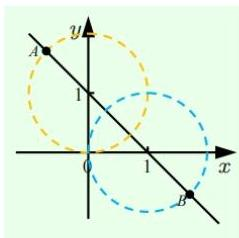
\includegraphics[max width=0.2\textwidth]{images/bo_d5jma53ef24c73bll4ig_141_1211_511_239_238_0.jpg}
\end{center}
\hspace*{3em} 

【解析】法一:若 \(\left| {{z}_{1} - 1}\right|  = 1\) ,

则复数 \({z}_{1}\) 在复平面的轨迹是以 \(\left( {1,0}\right)\) 为圆心,半径为 1 的圆.

\({z}_{1} = \mathrm{i}\overline{{z}_{2}} \Rightarrow  \left| {\mathrm{i}\overline{{z}_{2}} - 1}\right|  = 1 \Rightarrow  \left| {\overline{{z}_{2}} + \mathrm{i}}\right|  = 1 \Rightarrow  \left| {{z}_{2} - \mathrm{i}}\right|  = 1\) ,

则复数 \({z}_{2}\) 在复平面的轨迹是以 \(\left( {0,1}\right)\) 为圆心,半径为 1 的圆,

所以 \(\left| {{z}_{1} - {z}_{2}}\right|  \in  \left\lbrack  {0,2 + \sqrt{2}}\right\rbrack\) .

法二: 设 \({z}_{1} - 1 = \cos \theta  + i\sin \theta ,{z}_{2} = \frac{\cos \theta  + 1 + i\sin \theta }{i} = \sin \theta  + \mathrm{i}\left( {\cos \theta  + 1}\right)\) ,

则 \({\left| {z}_{1} - {z}_{2}\right| }^{2} = 2{\left( -\sin \theta  + \cos \theta  + 1\right) }^{2} \Rightarrow  \left| {{z}_{1} - {z}_{2}}\right|  = \left| {2\cos \left( {\theta  + \frac{\pi }{4}}\right)  + \sqrt{2}}\right|\) ,

所以 \({\left| {z}_{1} - {z}_{2}\right| }^{2} = 2{\left( \sin \theta  + \cos \theta  + 1\right) }^{2} \Rightarrow  \left| {{z}_{1} - {z}_{2}}\right|  = \left| {2\sin \left( {\theta  + \frac{\pi }{4}}\right)  + \sqrt{2}}\right|\) ,

\(\therefore \left| {{z}_{1} - {z}_{2}}\right|  \in  \left\lbrack  {0,2 + \sqrt{2}}\right\rbrack\) .

法三: 设 \({z}_{1} = x + {yi}\) ,则 \(\overline{{z}_{2}} = \frac{{z}_{1}}{i} = y - {xi}\) ,所以 \(\overline{{z}_{2}} = \frac{{z}_{1}}{i} = y - {xi},\therefore {z}_{2} = y + {xi}\) ,

由 \(\left| {{z}_{1} - 1}\right|  = 1\) 得 \({\left( x - 1\right) }^{2} + {y}^{2} = 1\) ,而 \(\left| {{z}_{1} - {z}_{2}}\right|  = \sqrt{2}\left| {x - y}\right|\) ,

令 \(\left\{  {\begin{array}{l} x = \cos \theta  + 1 \\  y = \sin \theta  \end{array},\theta  \in  \lbrack 0,{2\pi })}\right.\) ,则 \(\left| {{z}_{1} - {z}_{2}}\right|  = \sqrt{2}\left| {\cos \theta  - \sin \theta  + 1}\right|\)

\(\left| {{z}_{1} - {z}_{2}}\right|  = \sqrt{2}\left| {\cos \theta  - \sin \theta  + 1}\right|  = \sqrt{2}\left| {\sqrt{2}\cos \left( {\theta  + \frac{\pi }{4}}\right)  + 1}\right|\) ,故 \(\left| {{z}_{1} - {z}_{2}}\right|  \in  \left\lbrack  {0,2 + \sqrt{2}}\right\rbrack\) .

法四: 设 \({z}_{1} = x + {yi}\) ,则 \(\overline{{z}_{2}} = \frac{{z}_{1}}{i} = y - {xi}\) ,所以 \(\overline{{z}_{2}} = \frac{{z}_{1}}{i} = y - {xi},\therefore {z}_{2} = y + {xi}\) ,

由 \(\left| {{z}_{1} - 1}\right|  = 1\) 得 \({\left( x - 1\right) }^{2} + {y}^{2} = 1\) ,而 \(\left| {{z}_{1} - {z}_{2}}\right|  = \sqrt{2}\left| {x - y}\right|\) ,

令 \(t = x - y\) ,即 \(x - y - t = 0\) ,由点到直线距离公式得 \(d = \frac{\left| 1 - 0 - t\right| }{\sqrt{2}} \leq  1\) ,

故 \(1 - \sqrt{2} \leq  t \leq  1 + \sqrt{2}\) ,故 \(\left| {{z}_{1} - {z}_{2}}\right|  = \sqrt{2}\left| t\right|  \in  \left\lbrack  {0,2 + \sqrt{2}}\right\rbrack\) .

【例题】2. (2020 上海秋考) 已知 \({\overrightarrow{a}}_{1},{\overrightarrow{a}}_{2},{\overrightarrow{b}}_{1},{\overrightarrow{b}}_{2},\cdots ,{\overrightarrow{b}}_{k}\left( {k \in  {N}^{ * }}\right)\) 是平面内两两互不相等的向量,满足 \(\mid  {\overrightarrow{a}}_{1} \; - \overrightarrow{{a}_{2}} \mid   = 1\) ，且 \(\left| {\overrightarrow{{a}_{i}} - \overrightarrow{{b}_{j}}}\right|  \in  \{ 1,2\}\) (其中 \(\mathrm{i} = 1,2,j = 1,2,\cdots ,k\text{ ) }\) ，则 \(k\) 的最大值是\_\_\_\_\_.

【答案】 6

\begin{center}
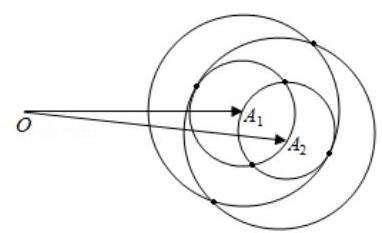
\includegraphics[max width=0.3\textwidth]{images/bo_d5jma53ef24c73bll4ig_141_1071_1653_382_233_0.jpg}
\end{center}
\hspace*{3em} 

【解析】如图,设 \(\overrightarrow{O{A}_{1}} = {\overrightarrow{a}}_{1},\overrightarrow{O{A}_{2}} = {\overrightarrow{a}}_{2}\) ,

由 \(\left| {{\overrightarrow{a}}_{1} - {\overrightarrow{a}}_{2}}\right|  = 1\) ,且 \(\left| {{\overrightarrow{a}}_{i} - {\overrightarrow{b}}_{j}}\right|  \in  \{ 1,2\}\) ,

分别以 \({A}_{1}\text{ 、 }{A}_{2}\) 为圆心,以 1 和 2 为半径画圆,

其中任意两圆的公共点共有 6 个.

故满足条件的 \(k\) 的最大值为 6 .

【例题】3. (2018 上海秋考) 已知实数 \({x}_{1}\text{ 、 }{x}_{2}\text{ 、 }{y}_{1}\text{ 、 }{y}_{2}\) 满足: \({x}_{1}^{2} + {y}_{1}^{2} = 1,{x}_{2}^{2}\)

\(+ {y}_{2}^{2} = 1,{x}_{1}{x}_{2} + {y}_{1}{y}_{2} = \frac{1}{2}\) ,则 \(\frac{\left| {x}_{1} + {y}_{1} - 1\right| }{\sqrt{2}} + \frac{\left| {x}_{2} + {y}_{2} - 1\right| }{\sqrt{2}}\) 的最大值为\_\_\_\_\_.

【答案】 \(\sqrt{3} + \sqrt{2}\)

【解析】作出圆 \(O : {x}^{2} + {y}^{2} = 1\) ,与直线 \(l : x + y - 1 = 0\) ,

\begin{center}
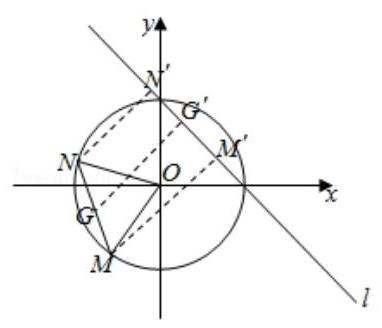
\includegraphics[max width=0.3\textwidth]{images/bo_d5jma53ef24c73bll4ig_142_1075_232_382_328_0.jpg}
\end{center}
\hspace*{3em} 

由题意得 \(M\left( {{x}_{1},{y}_{1}}\right) ,N\left( {{x}_{2},{y}_{2}}\right)\) 都在圆 \({x}^{2} + {y}^{2} = 1\) 上,

\(\left| {MN}\right|  = \sqrt{{\left( {x}_{1} - {x}_{2}\right) }^{2} + {\left( {y}_{1} - {y}_{2}\right) }^{2}} = 1\) ,则 \(\angle {MON} = {60}^{ \circ  }\) ,

\(\frac{\left| {x}_{1} + {y}_{1} - 1\right| }{\sqrt{2}} + \frac{\left| {x}_{2} + {y}_{2} - 1\right| }{\sqrt{2}}\) 表示 \(M\) 和 \(N\) 到直线 \(l : x + y - 1 = 0\)

的距离和

\(\left| {M{M}^{\prime }}\right|  + \left| {N{N}^{\prime }}\right| ,\)

由图像得只有当 \(M\text{ 、 }N\) 都在直线 \(l\) 的左侧距离之和才会取得最大值.

法一:取 \(M\text{ 、 }N\) 的中点 \(G\) ，过 \(G\) 作 \(G{G}^{\prime } \bot  l\) ，垂足为 \({G}^{\prime }\) ，

则 \(\left| {M{M}^{\prime }}\right|  + \left| {N{N}^{\prime }}\right|  = 2\left| {G{G}^{\prime }}\right|\) ,

因为 \(\bigtriangleup {MON}\) 为等边三角形, \(G\) 为 \({MN}\) 的中点,所以 \({OG} = \frac{\sqrt{3}}{2}\) ,

则 \(G\) 在圆 \({x}^{2} + {y}^{2} = \frac{3}{4}\) 上运动,故 \(G\) 到直线 \(x + y - 1 = 0\) 距离的最大值为 \(\frac{\sqrt{3}}{2} + \frac{\sqrt{2}}{2}\) ,

所以 \(\left| {M{M}^{\prime }}\right|  + \left| {N{N}^{\prime }}\right|  = 2\left| {G{G}^{\prime }}\right|\) 的最大值为 \(2 \times  \left( {\frac{\sqrt{3}}{2} + \frac{\sqrt{2}}{2}}\right)  = \sqrt{3} + \sqrt{2}\) ,

所以 \(\frac{\left| {x}_{1} + {y}_{1} - 1\right| }{\sqrt{2}} + \frac{\left| {x}_{2} + {y}_{2} - 1\right| }{\sqrt{2}}\) 的最大值为 \(\sqrt{3} + \sqrt{2}\) .

法二: 注意到 \(M\text{ 、 }N\) 都在直线 \(l\) 的左侧,

所以 \(\frac{\left| {x}_{1} + {y}_{1} - 1\right| }{\sqrt{2}} + \frac{\left| {x}_{2} + {y}_{2} - 1\right| }{\sqrt{2}} = \frac{1 - {x}_{1} - {y}_{1}}{\sqrt{2}} + \frac{1 - {x}_{2} - {y}_{2}}{\sqrt{2}}\) ,

可引入三角函数辅助计算,设 \(N\left( {\cos \alpha ,\sin \alpha }\right) ,M\left( {\cos \left( {\alpha  + \frac{\pi }{3}}\right) ,\sin \left( {\alpha  + \frac{\pi }{3}}\right) }\right)\) ,

则 \(\frac{\left| {x}_{1} + {y}_{1} - 1\right| }{\sqrt{2}} + \frac{\left| {x}_{2} + {y}_{2} - 1\right| }{\sqrt{2}} = \frac{1 - {x}_{1} - {y}_{1}}{\sqrt{2}} + \frac{1 - {x}_{2} - {y}_{2}}{\sqrt{2}}\)

\(= \sqrt{2} - \frac{1}{\sqrt{2}}\left\lbrack  {\cos \alpha  + \sin \alpha  + \cos \left( {\alpha  + \frac{\pi }{3}}\right)  + \sin \left( {\alpha  + \frac{\pi }{3}}\right) }\right\rbrack\)

\(= \sqrt{2} - \frac{1}{\sqrt{2}}\left( {\cos \alpha  + \sin \alpha  + \frac{1}{2}\cos \alpha  - \frac{\sqrt{3}}{2}\sin \alpha  + \frac{1}{2}\sin \alpha  + \frac{\sqrt{3}}{2}\cos \alpha }\right)\)

\(= \sqrt{2} - \frac{1}{\sqrt{2}}\left( {\frac{3 - \sqrt{3}}{2}\sin \alpha  + \frac{3 + \sqrt{3}}{2}\cos \alpha }\right)  = \sqrt{2} - \frac{1}{\sqrt{2}}\left( {\frac{3 - \sqrt{3}}{2}\sin \alpha  + \frac{3 + \sqrt{3}}{2}\cos \alpha }\right)\)

\(= \sqrt{2} - \frac{1}{\sqrt{2}}\sqrt{6}\sin \left( {\alpha  + \varphi }\right)  = \sqrt{2} - \sqrt{3}\sin \left( {\alpha  + \varphi }\right) ,\)

所以 \(\frac{\left| {x}_{1} + {y}_{1} - 1\right| }{\sqrt{2}} + \frac{\left| {x}_{2} + {y}_{2} - 1\right| }{\sqrt{2}}\) 的最大值为 \(\sqrt{3} + \sqrt{2}\) . 2025 版上海高考真题及模拟训练合集

\section*{B、数量积的多种计算选择}

\begin{center}
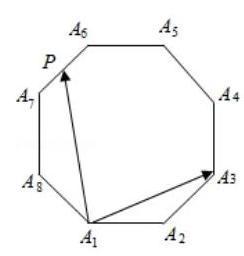
\includegraphics[max width=0.2\textwidth]{images/bo_d5jma53ef24c73bll4ig_143_1210_338_244_256_0.jpg}
\end{center}
\hspace*{3em} 

【例题】1. (2017上海春考)如图所示，正八边形 \({A}_{1}{A}_{2}{A}_{3}{A}_{4}{A}_{5}{A}_{6}{A}_{7}{A}_{8}\) 的边长为 2，若 \(P\) 为该正八边形边上的动点,则 \(\overrightarrow{{A}_{1}{A}_{3}} \cdot  \overrightarrow{{A}_{1}P}\) 的取值范围为 ( )

A. \(\left\lbrack  {0,8 + 6\sqrt{2}}\right\rbrack\) B. \(\left\lbrack  {-2\sqrt{2},8 + 6\sqrt{2}}\right\rbrack\)

C. \(\left\lbrack  {-8 - 6\sqrt{2},2\sqrt{2}}\right\rbrack\) D. \(\left\lbrack  {-8 - 6\sqrt{2},8 + 6\sqrt{2}}\right\rbrack\)

【答案】 \(B\)

【解析】正八边形 \({A}_{1}{A}_{2}{A}_{3}{A}_{4}{A}_{5}{A}_{6}{A}_{7}{A}_{8}\) 的每一个内角为 \({135}^{ \circ  }\) ,

且 \(\left| \overrightarrow{{A}_{1}{A}_{2}}\right|  = \left| \overrightarrow{{A}_{1}{A}_{8}}\right|  = 2,\left| \overrightarrow{{A}_{1}{A}_{3}}\right|  = \left| \overrightarrow{{A}_{1}{A}_{7}}\right|  = 2\sqrt{2 + \sqrt{2}}\) ,

\(\left| \overrightarrow{{A}_{1}{A}_{4}}\right|  = \left| \overrightarrow{{A}_{1}{A}_{6}}\right|  = 2 + 2\sqrt{2},\left| \overrightarrow{{A}_{1}{A}_{5}}\right|  = \sqrt{4 + 2\sqrt{2}}.\)

再由正弦函数的单调性及值域得,

当 \(P\) 与 \({A}_{8}\) 重合时, \(\overrightarrow{{A}_{1}{A}_{3}} \cdot  \overrightarrow{{A}_{1}P}\) 最小为

\(2 \times  2\sqrt{2 + \sqrt{2}} \times  \cos {112.5}^{ \circ  } = 2 \times  2\sqrt{2 + \sqrt{2}} \times  \left( {-\frac{\sqrt{2 - \sqrt{2}}}{2}}\right)  =  - 2\sqrt{2}\) .

结合选项得 \(\overrightarrow{{A}_{1}{A}_{3}} \cdot  \overrightarrow{{A}_{1}P}\) 的取值范围为 \(\left\lbrack  {-2\sqrt{2},8 + 6\sqrt{2}}\right\rbrack\) . 故选 \(B\) .

【例题】2. (2015 上海秋考) 在锐角三角形 \({ABC}\) 中, \(\tan A = \frac{1}{2},D\) 为边 \({BC}\) 上的点， \(\bigtriangleup  {ABD}\) 与 \(\bigtriangleup  {ACD}\) 的面积分别为2 和4. 过 \(D\) 作 \({DE}\bot {AB}\) 于 \(E,{DF}\bot {AC}\) 于 \(F\) ，则 \(\overrightarrow{DE} \cdot  \overrightarrow{DF} =\) \_\_\_\_\_.

【答案】 \(- \frac{16}{15}\)

【解析】因为 \(\bigtriangleup {ABD}\) 与 \(\bigtriangleup {ACD}\) 的面积分别为 2 和 4,

\begin{center}
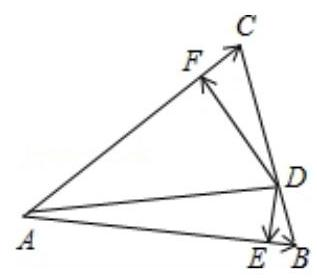
\includegraphics[max width=0.2\textwidth]{images/bo_d5jma53ef24c73bll4ig_143_1144_1125_317_278_0.jpg}
\end{center}
\hspace*{3em} 

所以 \(\frac{1}{2}\left| \overrightarrow{AB}\right|  \cdot  \left| \overrightarrow{DE}\right|  = 2,\frac{1}{2}\left| \overrightarrow{AC}\right|  \cdot  \left| \overrightarrow{DF}\right|  = 4\) ,

得 \(\left| \overrightarrow{DE}\right|  = \frac{4}{\left| \overrightarrow{AB}\right| },\left| \overrightarrow{DF}\right|  = \frac{8}{\left| \overrightarrow{AC}\right| }\) ,所以 \(\left| \overrightarrow{DE}\right|  \cdot  \left| \overrightarrow{DF}\right|  = \frac{32}{\left| \overrightarrow{AB}\right|  \cdot  \left| \overrightarrow{AC}\right| }\) .

又 \(\tan A = \frac{1}{2}\) ，所以 \(\frac{\sin A}{\cos A} = \frac{1}{2}\) ，联立 \({\sin }^{2}A + {\cos }^{2}A = 1\) ，

得 \(\sin A = \frac{\sqrt{5}}{5},\cos A = \frac{2\sqrt{5}}{5}\) ，

由 \(\frac{1}{2}\left| \overrightarrow{AB}\right|  \cdot  \left| \overrightarrow{AC}\right| \sin A = 6\) ,得 \(\left| \overrightarrow{AB}\right|  \cdot  \left| \overrightarrow{AC}\right|  = {12}\sqrt{5}\) ,则 \(\left| \overrightarrow{DE}\right|  \cdot  \left| \overrightarrow{DF}\right|  = \frac{8\sqrt{5}}{15}\) .

所以 \(\overrightarrow{DE} \cdot  \overrightarrow{DF} = \left| \overrightarrow{DE}\right|  \cdot  \left| \overrightarrow{DF}\right| \cos  < \overrightarrow{DE},\overrightarrow{DF} >  = \frac{8\sqrt{5}}{15} \times  \left( {-\frac{2\sqrt{5}}{5}}\right)  =  - \frac{16}{15}\) . 2025 版上海高考真题及模拟训练合集

\section*{C、多变量分析}

【例题】1. (2025 上海春考) 在平面上, \(\overrightarrow{{\mathrm{e}}_{1}}\) 和 \(\overrightarrow{{\mathrm{e}}_{2}}\) 是互相垂直的单位向量,向量 \(\overrightarrow{a}\) 满足 \(\left| {\overrightarrow{a} - 4\overrightarrow{{e}_{1}}}\right|  = 2\) ,向量 \(\overrightarrow{b}\) 满足 \(\left| {\overrightarrow{b} - 6{\overrightarrow{\mathrm{e}}}_{2}}\right|  = 1\) ，则 \(\overrightarrow{b}\) 在 \(\overrightarrow{a}\) 方向上的数量投影的最大值是\_\_\_\_\_.

【答案】 4

【解析】在平面直角坐标系中,设 \({\overrightarrow{\mathrm{e}}}_{1} = \left( {1,0}\right) ,{\overrightarrow{\mathrm{e}}}_{2} = \left( {0,1}\right)\) ,

由 \(\left| {\overrightarrow{a} - 4{\overrightarrow{e}}_{1}}\right|  = 2\) 和 \(\left| {\overrightarrow{b} - 6{\overrightarrow{\mathrm{e}}}_{2}}\right|  = 1\) ,

得 \(\overrightarrow{a}\) 的终点在圆 \(M : {\left( x - 4\right) }^{2} + {y}^{2} = 4\) 上, \(\overrightarrow{b}\) 的终点在圆 \(N : {x}^{2} + {\left( y - 6\right) }^{2} = 1\) 上,

设 \(\overrightarrow{a} = \overrightarrow{OA},\overrightarrow{b} = \overrightarrow{OB}\) ,

法一: \(\overrightarrow{b}\) 在 \(\overrightarrow{a}\) 方向上的数量投影为 \({OB}\cos \langle \overrightarrow{a},\overrightarrow{b}\rangle  \leq  {ON}\cos \left\langle  {\overrightarrow{ON},\overrightarrow{a}}\right\rangle   + 1\) ,

这个等号当且仅当 \({NB}\) 和 \(\overrightarrow{a}\) 平行时取等号,

要使得上式取最大值,则 \(\cos \langle \overrightarrow{ON},\overrightarrow{a}\rangle\) 最大, \(\left\langle  {\overrightarrow{ON},\overrightarrow{a}}\right\rangle\) 最小,

因此 \(\overrightarrow{a} = \overrightarrow{OA}\) 所在直线和圆 \(M : {\left( x - 4\right) }^{2} + {y}^{2} = 4\) 相切,

此时,由 \(\sin \angle {AOx} = \frac{1}{2}\) 得 \(\angle {AOx} = \frac{\pi }{6}\) ,则 \(< \overrightarrow{ON},\overrightarrow{a} >  = \frac{\pi }{3}\) ,

所以 \(\overrightarrow{b}\) 在 \(\overrightarrow{a}\) 方向上的数量投影的最大值是 \(6\cos \frac{\pi }{3} + 1 = 4\) .

法二: 设 \(\overrightarrow{a} = \left( {4 + 2\cos \alpha ,2\sin \alpha }\right) ,\overrightarrow{b} = \left( {\cos \beta ,6 + \sin \beta }\right)\) ,

\(\overrightarrow{b}\) 在 \(\overrightarrow{a}\) 方向上的数量投影 \(\left| \overrightarrow{b}\right| \cos  < \overrightarrow{a},\overrightarrow{b} >  = \frac{\overrightarrow{a} \cdot  \overrightarrow{b}}{\left| \overrightarrow{a}\right| }\)

\(= \frac{\left( {4 + 2\cos \alpha }\right) \cos \beta  + 2\sin \alpha \left( {6 + \sin \beta }\right) }{\sqrt{{\left( 4 + 2\cos \alpha \right) }^{2} + {\left( 2\sin \alpha \right) }^{2}}}\)

\(= \frac{\left( {4 + 2\cos \alpha }\right) \cos \beta  + 2\sin \alpha \sin \beta  + {12}\sin \alpha }{\sqrt{{20} + {16}\cos \alpha }},\)

\(\frac{{12}\left| {\sin \alpha }\right| }{\sqrt{{20} + {16}\cos \alpha }} = \frac{{12}\left| {\sin \alpha }\right| }{4\sqrt{\cos \alpha  + \frac{5}{4}}} = 3\sqrt{\frac{{\sin }^{2}\alpha }{\cos \alpha  + \frac{5}{4}}}\)

\(= 3\sqrt{\frac{1 - {\cos }^{2}\alpha }{\cos \alpha  + \frac{5}{4}}} = 3\sqrt{\frac{1 - {\left( \cos \alpha  + \frac{5}{4} - \frac{5}{4}\right) }^{2}}{\cos \alpha  + \frac{5}{4}}}\)

\(= 3\sqrt{\frac{1 - {\left( \cos \alpha  + \frac{5}{4}\right) }^{2} + \frac{5}{2}\left( {\cos \alpha  + \frac{5}{4}}\right)  - \frac{25}{16}}{\cos \alpha  + \frac{5}{4}}} = 3\sqrt{\frac{5}{2} - \left( {\cos \alpha  + \frac{5}{4}}\right)  - \frac{\frac{9}{16}}{\cos \alpha  + \frac{5}{4}}}\)

\(\leq  3\sqrt{\frac{5}{2} - 2\sqrt{\left( {\cos \alpha  + \frac{5}{4}}\right)  \times  \frac{\frac{9}{16}}{\cos \alpha  + \frac{5}{4}}}} = 3\) ,即 \(\frac{{12}\left| {\sin \alpha }\right| }{\sqrt{{20} + {16}\cos \alpha }} \leq  3\) ,

其中等号当且仅当 \(\cos \alpha  + \frac{5}{4} = \frac{\frac{9}{16}}{\cos \alpha  + \frac{5}{4}}\) ,即 \(\cos \alpha  =  - \frac{1}{2}\) 时成立,

由此可得 \(- 3 \leq  \frac{{12}\sin \alpha }{\sqrt{{20} + {16}\cos \alpha }} \leq  3\) ,

当且仅当 \(\cos \alpha  =  - \frac{1}{2}\) 且 \(\sin \alpha  =  - \frac{\sqrt{3}}{2}\) 时, \(\frac{{12}\sin \alpha }{\sqrt{{20} + {16}\cos \alpha }} =  - 3\) ;

当且仅当 \(\cos \alpha  =  - \frac{1}{2}\) 且 \(\sin \alpha  = \frac{\sqrt{3}}{2}\) 时, \(\frac{{12}\sin \alpha }{\sqrt{{20} + {16}\cos \alpha }} = 3\) .

所以 \(\left| \overrightarrow{b}\right| \cos  < \overrightarrow{a},\overrightarrow{b} >  = \frac{\overrightarrow{a} \cdot  \overrightarrow{b}}{\left| \overrightarrow{a}\right| } = \frac{\left( {4 + 2\cos \alpha }\right) \cos \beta  + 2\sin \alpha \sin \beta  + {12}\sin \alpha }{\sqrt{{20} + {16}\cos \alpha }}\)

\(\leq  \frac{\sqrt{{\left( 4 + 2\cos \alpha \right) }^{2} + {\left( 2\sin \alpha \right) }^{2}} + {12}\sin \alpha }{\sqrt{{20} + {16}\cos \alpha }} = 1 + \frac{{12}\sin \alpha }{\sqrt{{20} + {16}\cos \alpha }},\)

其中等号当且仅当 \(\sin \beta  = \frac{2\sin \alpha }{\sqrt{{\left( 4 + 2\cos \alpha \right) }^{2} + {\left( 2\sin \alpha \right) }^{2}}}\) ,

\(\sin \beta  = \frac{2\sin \alpha }{\sqrt{{\left( 4 + 2\cos \alpha \right) }^{2} + {\left( 2\sin \alpha \right) }^{2}}},\cos \beta  = \frac{4 + 2\cos \alpha }{\sqrt{{\left( 4 + 2\cos \alpha \right) }^{2} + {\left( 2\sin \alpha \right) }^{2}}}\) 时成立,

则 \(\left| \overrightarrow{b}\right| \cos  < \overrightarrow{a},\overrightarrow{b} >  \leq  1 + 3 = 4\) ,

其中等号当且仅当 \(\sin \beta  = \frac{1}{2}\) 时成立,

所以,当 \(\overrightarrow{a} = \left( {3,\sqrt{3}}\right) ,\overrightarrow{b} = \left( {\frac{\sqrt{3}}{2},\frac{13}{2}}\right)\) 时, \(\left| \overrightarrow{b}\right| \cos  < \overrightarrow{a},\overrightarrow{b} >\) 取得最大值 4,

所以 \(\overrightarrow{b}\) 在 \(\overrightarrow{a}\) 方向上的数量投影的最大值是 \(6\cos \frac{\pi }{3} + 1 = 4\) .

法三: 自由向量分析,设 \(\overrightarrow{a} - 4{\overrightarrow{\mathrm{e}}}_{1} = 2\overrightarrow{m},\overrightarrow{b} - 6{\overrightarrow{\mathrm{e}}}_{2} = \overrightarrow{n}\) ,则 \(\left| \overrightarrow{m}\right|  = \left| \overrightarrow{n}\right|  = 1\) ,

故 \(\overrightarrow{b} \cdot  \overrightarrow{a} = 4{\overrightarrow{\mathrm{e}}}_{1} \cdot  \overrightarrow{n} + {12}{\overrightarrow{\mathrm{e}}}_{2} \cdot  \overrightarrow{m} + 2\overrightarrow{m} \cdot  \overrightarrow{n},\left| \overrightarrow{a}\right|  = 2\sqrt{5 + 4{\overrightarrow{\mathrm{e}}}_{1} \cdot  \overrightarrow{m}}\) ,

则 \(\frac{\overrightarrow{b} \cdot  \overrightarrow{a}}{\left| \overrightarrow{a}\right| } = \frac{2\overrightarrow{{\mathrm{e}}_{1}} \cdot  \overrightarrow{n} + 6\overrightarrow{{\mathrm{e}}_{2}} \cdot  \overrightarrow{m} + \overrightarrow{m} \cdot  \overrightarrow{n}}{\sqrt{5 + 4\overrightarrow{{\mathrm{e}}_{1}} \cdot  \overrightarrow{m}}} = \frac{\left( {2\overrightarrow{{\mathrm{e}}_{1}} + \overrightarrow{m}}\right)  \cdot  \overrightarrow{n} + 6\overrightarrow{{\mathrm{e}}_{2}} \cdot  \overrightarrow{m}}{\sqrt{5 + 4\overrightarrow{{\mathrm{e}}_{1}} \cdot  \overrightarrow{m}}}\)

\(\leq  \frac{\left| {2\overrightarrow{{\mathrm{e}}_{1}} + \overrightarrow{m}}\right|  + 6\overrightarrow{{\mathrm{e}}_{2}} \cdot  \overrightarrow{m}}{\sqrt{5 + 4\overrightarrow{{\mathrm{e}}_{1}} \cdot  \overrightarrow{m}}} = \frac{\sqrt{5 + 4\overrightarrow{{\mathrm{e}}_{1}} \cdot  \overrightarrow{m}} + 6\overrightarrow{{\mathrm{e}}_{2}} \cdot  \overrightarrow{m}}{\sqrt{5 + 4\overrightarrow{{\mathrm{e}}_{1}} \cdot  \overrightarrow{m}}} = 1 + \frac{6\overrightarrow{{\mathrm{e}}_{2}} \cdot  \overrightarrow{m}}{\sqrt{5 + 4\overrightarrow{{\mathrm{e}}_{1}} \cdot  \overrightarrow{m}}},\)

设 \({\overrightarrow{\mathrm{e}}}_{1} = \left( {1,0}\right) ,{\overrightarrow{\mathrm{e}}}_{2} = \left( {0,1}\right) ,\overrightarrow{m} = \left( {\cos \theta ,\sin \theta }\right)\) ,则 \(\frac{6{\overrightarrow{\mathrm{e}}}_{2} \cdot  \overrightarrow{m}}{\sqrt{5 + 4{\overrightarrow{\mathrm{e}}}_{1} \cdot  \overrightarrow{m}}} = \frac{6\sin \theta }{\sqrt{5 + 4\cos \theta }}\) ,

令 \(t = 5 + 4\cos \theta  \in  \left\lbrack  {1,9}\right\rbrack\) ,则 \(\frac{6\sin \theta }{\sqrt{5 + 4\cos \theta }} \leq  6\sqrt{\frac{1 - {\cos }^{2}\theta }{5 + 4\cos \theta }} = 6\sqrt{\frac{1 - {\left( \frac{t - 5}{4}\right) }^{2}}{t}}\)

\(= 6\sqrt{\frac{{16} - \left( {{t}^{2} - {10t} + {25}}\right) }{16t}} = 6\sqrt{\frac{10}{16} - \frac{1}{16}\left( {t + \frac{9}{t}}\right) } \leq  6\sqrt{\frac{10}{16} - \frac{6}{16}} = 3\) ,

所以 \(\frac{\overrightarrow{b} \cdot  \overrightarrow{a}}{\left| \overrightarrow{a}\right| } \leq  1 + 3 = 4\) ,所以 \(\overrightarrow{b}\) 在 \(\overrightarrow{a}\) 方向上的数量投影的最大值是 \(6\cos \frac{\pi }{3} + 1 = 4\) .

【例题】2. (2014 上海秋考) 已知曲线 \(C : x =  - \sqrt{4 - {y}^{2}}\) ，直线 \(l : x = 6\) ，若对于点 \(A\left( {m,0}\right)\) ，存在 \(C\) 上的点 \(P\) 和 \(l\) 上的 \(Q\) 使得 \(\overrightarrow{AP} + \overrightarrow{AQ} = \overrightarrow{0}\) ，则 \(m\) 的取值范围为\_\_\_\_\_.

【答案】 \(\left\lbrack  {2,3}\right\rbrack\)

【解析】曲线 \(C : x =  - \sqrt{4 - {y}^{2}}\) ,是以原点为圆心,2 为半径的圆,并且 \({x}_{P} \in  \left\lbrack  {-2,0}\right\rbrack\) , 对于点 \(A\left( {m,0}\right)\) ,存在 \(C\) 上的点 \(P\) 和 \(l\) 上的 \(Q\) 使得 \(\overrightarrow{AP} + \overrightarrow{AQ} = \overrightarrow{0}\) , 说明 \(A\) 是 \({PQ}\) 的中点, \(Q\) 的横坐标 \(x = 6\) ,所以 \(m = \frac{6 + {x}_{P}}{2} \in  \left\lbrack  {2,3}\right\rbrack\) .

【例题】3. (2013上海秋考)在边长为 1 的正六边形 \({ABCDEF}\) 中，记以 \(A\) 为起点，其余顶点为终点的向量分别为 \({\overrightarrow{a}}_{1}\text{ 、 }{\overrightarrow{a}}_{2}\text{ 、 }{\overrightarrow{a}}_{3}\text{ 、 }{\overrightarrow{a}}_{4}\text{ 、 }{\overrightarrow{a}}_{5}\) ; 以 \(D\) 为起点,其余顶点为终点的向量分别为 \({\overrightarrow{d}}_{1}\text{ 、 }{\overrightarrow{d}}_{2}\text{ 、 }{\overrightarrow{d}}_{3}\text{ 、 }{\overrightarrow{d}}_{4}\text{ 、 }{\overrightarrow{d}}_{5}\) . 若 \(m\text{ 、 }M\) 分别为 \(\left( {{\overrightarrow{a}}_{i} + {\overrightarrow{a}}_{j} + {\overrightarrow{a}}_{k}}\right)  \cdot  \left( {{\overrightarrow{d}}_{r} + {\overrightarrow{d}}_{s} + {\overrightarrow{d}}_{t}}\right)\) 的最小值、最大值,其中 \(\{ i,j,k\}  \subseteq  \{ 1,2,3,4,5\} ,\{ r,s,t\}\)

\(\subseteq  \{ 1,2,3,4,5\}\) ,则 \(m\text{ 、 }M\) 满足 ( )

A. \(m = 0,M > 0\) B. \(m < 0,M > 0\) C. \(m < 0,M = 0\) D. \(m < 0,M < 0\)

【答案】 \(D\)

【解析】由题意得以 \(A\) 为起点,其余顶点为终点的向量分别为 \({\overrightarrow{a}}_{1}\text{ 、 }{\overrightarrow{a}}_{2}\text{ 、 }{\overrightarrow{a}}_{3}\text{ 、 }{\overrightarrow{a}}_{4}\text{ 、 }{\overrightarrow{a}}_{5}\) ;

以 \(D\) 为起点,其余顶点为终点的向量分别为 \({\overrightarrow{d}}_{1}\text{ 、 }{\overrightarrow{d}}_{2}\text{ 、 }{\overrightarrow{d}}_{3}\text{ 、 }{\overrightarrow{d}}_{4}\text{ 、 }{\overrightarrow{d}}_{5}\) ,

由向量的数量积公式,只有 \(\overrightarrow{AF} \cdot  \overrightarrow{DE} = \overrightarrow{AB} \cdot  \overrightarrow{DC} > 0\) ,其余数量积均小于等于 0,

因为 \(m\text{ 、 }M\) 分别为 \(\left( {{\overrightarrow{a}}_{i} + {\overrightarrow{a}}_{j} + {\overrightarrow{a}}_{k}}\right)  \cdot  \left( {{\overrightarrow{d}}_{r} + {\overrightarrow{d}}_{s} + {\overrightarrow{d}}_{t}}\right)\) 的最小值、最大值,

所以 \(m < 0,M < 0\) ,故选 \(D\) .

\begin{center}
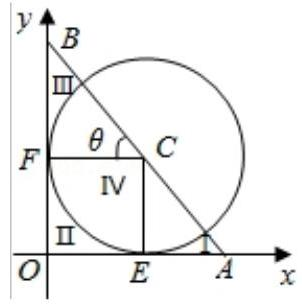
\includegraphics[max width=0.2\textwidth]{images/bo_d5jma53ef24c73bll4ig_146_1151_672_302_306_0.jpg}
\end{center}
\hspace*{3em} 

【例题】4. (2009 上海秋考) 过圆 \(C : {\left( x - 1\right) }^{2} + {\left( y - 1\right) }^{2} = 1\) 的圆心,作直线分别交 \(x\text{ 、 }y\) 轴正半轴于点 \(A\text{ 、 }B,{\Delta AOB}\) 被圆分成四部分 (如图),若这四部分图形面积满足 \({S}_{I} + {S}_{IV} = {S}_{II} + {S}_{III}\) 则直线 \({AB}\) 有 ( )

A. 0 条 B. 1 条

C. 2 条 D. 3 条

【答案】 \(B\)

【解析】由题意得 \({S}_{IV} - {S}_{II} = {S}_{III} - {S}_{I}\) ,由图形得第 \({II}\text{ 、 }{IV}\) 部分的面积分别为 \({S}_{\text{ 正方形 }{OECF}} - {S}_{\text{ 扇形 }{ECF}} = 1 - \frac{\pi }{4}\) 和 \({S}_{\text{ 扇形 }{ECF}} = \frac{\pi }{4}\) ,

所以 \({S}_{IV} - {S}_{II}\) 为定值,即 \({S}_{III} - {S}_{I}\) 为定值,

当直线 \({AB}\) 绕着圆心 \(C\) 移动时,只可能有一个位置符合题意,即直线 \({AB}\) 只有一条. 故选 B. 2025 版上海高考真题及模拟训练合集

\section*{2. 模拟练习}

【练习】1. 已知 \(\left| \overrightarrow{a}\right|  = \left| \overrightarrow{b}\right|  = 1,\overrightarrow{a} \cdot  \overrightarrow{b} = \frac{1}{2},\overrightarrow{c} = \left( {m,1 - m}\right) ,\overrightarrow{d} = \left( {n,1 - n}\right) \left( {m,n \in  R}\right)\) . 存在 \(\overrightarrow{a}\text{ 、 }\overrightarrow{b}\) ,对于任意实数 \(m,n\) ，不等式 \(\left| {\overrightarrow{a} - \overrightarrow{c}}\right|  + \left| {\overrightarrow{b} - \overrightarrow{d}}\right|  \geq  T\) 成立，则实数 \(T\) 的取值范围为\_\_\_\_\_.

【答案】 \(( - \infty ,\sqrt{3} + \sqrt{2}\rbrack\)

【解析】由题意得 \(\overrightarrow{a}\text{ 、 }\overrightarrow{b}\) 的夹角为 \(\frac{\pi }{3}\) .

\begin{center}
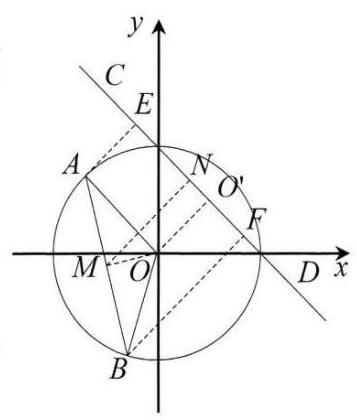
\includegraphics[max width=0.3\textwidth]{images/bo_d5jma53ef24c73bll4ig_147_1099_523_357_420_0.jpg}
\end{center}
\hspace*{3em} 

可设 \(\overrightarrow{a} = \overrightarrow{OA},\overrightarrow{b} = \overrightarrow{OB},\overrightarrow{c} = \overrightarrow{OC},\overrightarrow{d} = \overrightarrow{OD}\) ,

则点 \(A\text{ 、 }B\) 在单位圆上,点 \(C\text{ 、 }D\) 在直线 \(x + y - 1 = 0\) 上,由 \(m\text{ 、 }n\) 的任意性,

即求点 \(A\text{ 、 }B\) 到直线 \(x + y - 1 = 0\) 距离之和的最小值,

即 \(\left| {AE}\right|  + \left| {BF}\right|\) (点 \(E\text{ 、 }F\) 分别是点 \(A\text{ 、 }B\) 在直线

\(x + y - 1 = 0\) 上的射影点);

同时根据 \(\overrightarrow{a},\overrightarrow{b}\) 的存在性,问题转化为求 \(\left| {AE}\right|  + \left| {AF}\right|\) 的最大值.

设 \({AB}\) 的中点为 \(M\) ,设点 \(M\text{ 、 }O\) 在直线 \(x + y - 1 = 0\) 上射影点分别为 \(N\text{ 、 }{O}^{\prime }\) ,

则 \(\left| {AE}\right|  + \left| {BF}\right|  = 2\left| {MN}\right|  \leq  2\left( {\left| {MO}\right|  + \left| {O{O}^{\prime }}\right| }\right)  = 2\left( {\frac{\sqrt{3}}{2} + \frac{\sqrt{2}}{2}}\right)  = \; \sqrt{3} + \sqrt{2}\) ,

当且仅当点 \(M\text{ 、 }O\text{ 、 }{O}^{\prime }\) 依次在一条直线上时取等号.

所以 \(T \leq  \sqrt{3} + \sqrt{2}\) ,则实数 \(T\) 的取值范围为 \(( - \infty ,\sqrt{3} + \sqrt{2}\rbrack\) .

【练习】2. (2025 届交附) 在边长为 1 的正六边形 \({ABDEFG}\) 中,以 \(A\) 为起点其它 5 个顶点之一为终点的向量分别记为 \({\overrightarrow{a}}_{1},{\overrightarrow{a}}_{2},{\overrightarrow{a}}_{3},{\overrightarrow{a}}_{4},{\overrightarrow{a}}_{5}\) ,以 \(D\) 为起点其它 5 个顶点之一为终点的向量分别记为 \({\overrightarrow{d}}_{1},{\overrightarrow{d}}_{2}\) 、 \({\overrightarrow{d}}_{3},{\overrightarrow{d}}_{4},{\overrightarrow{d}}_{5}\) . 若 \(m,M\) 分别为 \(\left( {{\overrightarrow{a}}_{l} + {\overrightarrow{a}}_{j} + {\overrightarrow{a}}_{k}}\right)  \cdot  \left( {{\overrightarrow{d}}_{r} + {\overrightarrow{d}}_{s} + {\overrightarrow{d}}_{l}}\right)\) 的最小值、最大值,其中 \(\{ \mathrm{i},j,k\}  \subset  \{ 1,2,3\) , \(4,5\} ,\{ r,s,t\}  \subset  \{ 1,2,3,4,5\}\) ,则 \(m + M\) 的值为\_\_\_\_\_

【答案】 -13

【解析】建立平面直角坐标系如图所示,

则 \({\overrightarrow{a}}_{1} = \overrightarrow{AB} = \left( {\frac{\sqrt{3}}{2}, - \frac{1}{2}}\right) ,{\overrightarrow{a}}_{1} = \overrightarrow{DB} = \left( {-\frac{\sqrt{3}}{2}, - \frac{1}{2}}\right)\) ,

\begin{center}
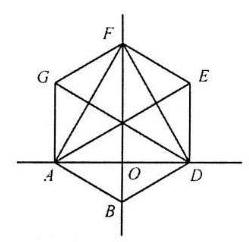
\includegraphics[max width=0.2\textwidth]{images/bo_d5jma53ef24c73bll4ig_147_295_1526_249_242_0.jpg}
\end{center}
\hspace*{3em} 

\({\overrightarrow{a}}_{2} = \overrightarrow{AD} = \left( {\sqrt{3},0}\right) ,{\overrightarrow{d}}_{2} = \overrightarrow{DA} = \left( {-\sqrt{3},0}\right) ,\)

\(\overline{{a}_{3}} = \overline{AE} = \left( {\sqrt{3},1}\right) ,\overline{{d}_{3}} = \overline{DG} = \left( {-\sqrt{3},1}\right) ,\)

\({\overrightarrow{a}}_{4} = \overrightarrow{AF} = \left( {\frac{\sqrt{3}}{2},\frac{3}{2}}\right) ,{\overrightarrow{d}}_{4} = \overrightarrow{DF} = \left( {-\frac{\sqrt{3}}{2},\frac{3}{2}}\right) ,\)

\({\overrightarrow{a}}_{5} = \overrightarrow{AG} = \left( {0,1}\right) ,{\overrightarrow{d}}_{5} = \overrightarrow{DE} = \left( {0,1}\right) ,\)

下面计算 \(\left( {{\overrightarrow{a}}_{l} + {\overrightarrow{a}}_{j} + {\overrightarrow{a}}_{k}}\right)  \cdot  \left( {{\overrightarrow{d}}_{r} + {\overrightarrow{d}}_{s} + {\overrightarrow{d}}_{t}}\right)\)

任取 \({\overrightarrow{a}}_{i}\left( {\mathrm{i} = 1,2,3,4,5}\right)\) 中三个作和,横坐标都是正的,纵坐标也是正,任取 \({\bar{d}}_{i}\left( {\mathrm{i} = 1,2,3,4,5}\right)\) 中的

三个作和，横坐标全是负的，纵坐标全是正的. 为了取得数量积的最小值， \({\overrightarrow{a}}_{i} + {\overrightarrow{a}}_{j} + {\overrightarrow{a}}_{k}\) 和的横坐标最大,纵坐标最小,而 \({\overrightarrow{d}}_{t} + {\overrightarrow{d}}_{s} + {\overrightarrow{d}}_{t}\) 和的横坐标 (负的) 绝对值最大,纵坐标最小即可

因此 \(m = \left( {\overrightarrow{AB} + \overrightarrow{AD} + \overrightarrow{AE}}\right)  \cdot  \left( {\overrightarrow{DB} + \overrightarrow{DA} + \overrightarrow{DG}}\right)  = \left( {\frac{5\sqrt{3}}{2},\frac{1}{2}}\right)  \cdot  \left( {-\frac{5\sqrt{3}}{2},\frac{1}{2}}\right)  =  - \frac{37}{2}\) ,为了取得数量积的最大值, \({\overrightarrow{a}}_{i} + {\overrightarrow{a}}_{j} + {\overrightarrow{a}}_{k}\) 和的横坐标最小,纵坐标最大,而 \({\overrightarrow{d}}_{r} + {\overrightarrow{d}}_{s} + {\overrightarrow{d}}_{t}\) 和的横坐标 (负的) 绝对值最小,纵坐标最大即可

因此 \(M = \left( {\overrightarrow{AE} + \overrightarrow{AF} + \overrightarrow{AG}}\right)  \cdot  \left( {\overrightarrow{DG} + \overrightarrow{DF} + \overrightarrow{DE}}\right)  = \left( {\frac{3\sqrt{3}}{2},\frac{7}{2}}\right)  \cdot  \left( {-\frac{3\sqrt{3}}{2},\frac{7}{2}}\right)  = \frac{11}{2}\) ,所以 \(m + M \; =  - \frac{37}{2} + \frac{11}{2} =  - {13}\)

【练习】3. (2024 届华二)已知 \(\bigtriangleup  {ABC}\) 是边长为 4 的正三角形，平面上两动点 \(O\) ， \(P\) 满足 \(\overrightarrow{OP} = {\lambda }_{1}\overrightarrow{OA} + \; {\lambda }_{2}\overrightarrow{OB} + {\lambda }_{3}\overrightarrow{OC}\left( {{\lambda }_{1} + {\lambda }_{2} + {\lambda }_{3} = 1\text{ 且 }{\lambda }_{1},{\lambda }_{2},{\lambda }_{3} \geq  0}\right)\) . 若 \(\left| \overrightarrow{OP}\right|  = 1\) ，则 \(\overrightarrow{OA} \cdot  \overrightarrow{OB}\) 的最大值为\_\_\_\_\_.

【答案】 \(9 + 4\sqrt{3}\)

【解析】由已知 \(\overrightarrow{OP} = {\lambda }_{1}\overrightarrow{OA} + {\lambda }_{2}\overrightarrow{OB} + {\lambda }_{3}\overrightarrow{OC},{\lambda }_{1} + {\lambda }_{2} + {\lambda }_{3} = 1\) ,

\begin{center}
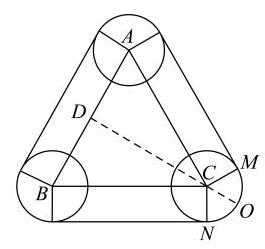
\includegraphics[max width=0.2\textwidth]{images/bo_d5jma53ef24c73bll4ig_148_1191_850_265_249_0.jpg}
\end{center}
\hspace*{3em} 

则 \(\overrightarrow{OP} = {\lambda }_{1}\left( {\overrightarrow{OP} + \overrightarrow{PA}}\right)  + {\lambda }_{2}\left( {\overrightarrow{OP} + \overrightarrow{PB}}\right)  + {\lambda }_{3}\left( {\overrightarrow{OP} + \overrightarrow{PC}}\right)\) ,

则 \({\lambda }_{1}\overrightarrow{PA} + {\lambda }_{2}\overrightarrow{PB} + {\lambda }_{3}\overrightarrow{PC} = \overrightarrow{0}\) ,即 \({\lambda }_{1}\overrightarrow{PA} + {\lambda }_{2}\left( {\overrightarrow{PA} + \overrightarrow{AB}}\right)  + {\lambda }_{3}\left( {\overrightarrow{PA} + \overrightarrow{AC}}\right)  = \overrightarrow{0}\) ,

则 \(\overrightarrow{AP} = {\lambda }_{2}\overrightarrow{AB} + {\lambda }_{3}\overrightarrow{AC}\) ,又 \({\lambda }_{1} + {\lambda }_{2} + {\lambda }_{3} = 1\) ,且 \({\lambda }_{1},{\lambda }_{2},{\lambda }_{3} \geq  0\) ,

则 \(0 \leq  {\lambda }_{2} + {\lambda }_{3} \leq  1\) ,则点 \(P\) 在 \(\bigtriangleup {ABC}\) 内部或边上,

又 \(\left| \overrightarrow{OP}\right|  = 1\) ，所以点 \(O\) 在以 \(P\) 为圆心，1为半径的圆上，设 \({AB}\) 中点为 \(D\) ，

则 \(\overrightarrow{OA} \cdot  \overrightarrow{OB} = \left( {\overrightarrow{OD} + \overrightarrow{DA}}\right)  \cdot  \left( {\overrightarrow{OD} + \overrightarrow{DB}}\right)  = {\overrightarrow{OD}}^{2} - {\overrightarrow{AD}}^{2} = {\overrightarrow{OD}}^{2} - 4\) ，

易得当点 \(O\) 为直线 \({DC}\) 与 \(\overset{\text{ ⏜ }}{MN}\) 交点时, \({OD}\) 最大为 \(2\sqrt{3} + 1\) ,

即 \(\overrightarrow{OA} \cdot  \overrightarrow{OB} = {\overrightarrow{OD}}^{2} - 4\) 的最大值为 \({\left( 2\sqrt{3} + 1\right) }^{2} - 4 = 9 + 4\sqrt{3}\) .

【练习】4. (2025 届复兴) 已如平面向量 \({\overrightarrow{a}}_{1},{\overrightarrow{a}}_{2},{\overrightarrow{a}}_{3},{\overrightarrow{a}}_{4},{\overrightarrow{a}}_{5},{\overrightarrow{a}}_{6}\) 两两都不共线. 若 \(\left| {\overrightarrow{a}}_{1}\right|  = \left| {{\overrightarrow{a}}_{i} - \overrightarrow{{a}_{i + 1}}}\right|  = 1\) , \({\overrightarrow{a}}_{i} \cdot  \overrightarrow{{a}_{i + 1}} = \frac{\sqrt{3}}{2}\left| {\overrightarrow{a}}_{i}\right|  \cdot  \left| \overrightarrow{{a}_{i + 1}}\right| \left( {\mathrm{i} \in  \{ 1,2,3,4,5\} }\right)\) ,则 \({\overrightarrow{a}}_{1} \cdot  \left( {{\overrightarrow{a}}_{2} + {\overrightarrow{a}}_{3} + {\overrightarrow{a}}_{4} + {\overrightarrow{a}}_{3} + {\overrightarrow{a}}_{6}}\right)\) 的最大值是\_\_\_\_\_.

【答案】 \(\frac{1}{2}\)

【解析】由于 \(\left| \overrightarrow{{a}_{1}}\right|  = 1\) ,于是 \(\overrightarrow{{a}_{1}} \cdot  \left( {\overrightarrow{{a}_{2}} + \overrightarrow{{a}_{3}} + \overrightarrow{{a}_{4}} + \overrightarrow{{a}_{3}} + \overrightarrow{{a}_{6}}}\right)\) 的最大值就是 \(\overrightarrow{{a}_{2}},\overrightarrow{{a}_{3}},\overrightarrow{{a}_{4}},\overrightarrow{{a}_{5}},\overrightarrow{{a}_{6}}\)

\begin{center}
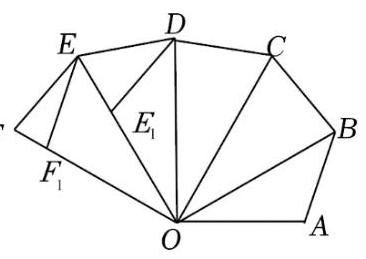
\includegraphics[max width=0.3\textwidth]{images/bo_d5jma53ef24c73bll4ig_148_1090_1523_366_259_0.jpg}
\end{center}
\hspace*{3em} 

在 \({\overrightarrow{a}}_{1}\) 上的投影之和最大值,

由 \(\left| \overrightarrow{{a}_{1}}\right|  = \left| {\overrightarrow{{a}_{i}} - \overrightarrow{{a}_{i + 1}}}\right|  = 1,\overrightarrow{{a}_{i}} \cdot  \overrightarrow{{a}_{i + 1}} = \frac{\sqrt{3}}{2}\left| \overrightarrow{{a}_{i}}\right|  \cdot  \left| \overrightarrow{{a}_{i + 1}}\right|\) 得,相邻两向量夹角为 \(\frac{\pi }{6}\) ,以相邻两向量的模为边长的第三边长度为 1,取 \(\overrightarrow{{a}_{1}}F \; = \overrightarrow{OA}\) ,

作出图象如图所示,则 \(\overrightarrow{OB} = {\overrightarrow{a}}_{2},\overrightarrow{OD} = {\overrightarrow{a}}_{4},\overrightarrow{O{F}_{1}} = {\overrightarrow{a}}_{6}\) ,

当 \(\overrightarrow{{a}_{3}} = \overrightarrow{OC},\overrightarrow{{a}_{5}} = \overrightarrow{O{E}_{1}}\) 时，所有向量在 \(\overrightarrow{OA}\) 上的投影之和最大，

\({\overrightarrow{a}}_{1} \cdot  \left( {{\overrightarrow{a}}_{2} + {\overrightarrow{a}}_{3} + {\overrightarrow{a}}_{4} + {\overrightarrow{a}}_{3} + {\overrightarrow{a}}_{6}}\right)  \leq  \frac{3}{2} + 1 + 0 - \frac{1}{2} - \frac{3}{2} = \frac{1}{2}\) ,最大值为 \(\frac{1}{2}\) .

【练习】5. (2024 届复附) 若平面向量 \(\overrightarrow{a},\overrightarrow{b},\overrightarrow{a} + \overrightarrow{b}\) 的模均在区间 \(\left\lbrack  {2,4}\right\rbrack\) 内，则 \(\overrightarrow{a} \cdot  \overrightarrow{b}\) 的取值范围是\_\_\_\_\_. 【答案】 \(\left\lbrack  {-{14},4}\right\rbrack\)

【解析】 \(\overrightarrow{a} \cdot  \overrightarrow{b} = \frac{{\left( \overrightarrow{a} + \overrightarrow{b}\right) }^{2} - {\left| \overrightarrow{a}\right| }^{2} - {\left| \overrightarrow{b}\right| }^{2}}{2} \geq  \frac{{2}^{2} - {4}^{2} - {4}^{2}}{2} =  - {14}\) ,

等号成立当且且当 \(\left| \overrightarrow{a}\right|  = \left| \overrightarrow{b}\right|  = 4,\left| {\overrightarrow{a} + \overrightarrow{b}}\right|  = 2\) ,取边长为4,4,2的等腰 \(\bigtriangleup {OAB}\) ,

其中 \({AB} = 2\) ,令 \(\overrightarrow{OA} = \overrightarrow{a},\overrightarrow{BO} = \overrightarrow{b}\) 即可,

又 \(\overrightarrow{a} \cdot  \overrightarrow{b} = \frac{{\left( \overrightarrow{a} + \overrightarrow{b}\right) }^{2} - {\left( \overrightarrow{a} - \overrightarrow{b}\right) }^{2}}{4} \leq  \frac{{4}^{2}}{4} = 4\) ,取 \(\overrightarrow{a} = \overrightarrow{b} = \left( {2,0}\right)\) ,等号成立,

则 \(\overrightarrow{a} \cdot  \overrightarrow{b}\) 的取值范围是 \(\left\lbrack  {-{14},4}\right\rbrack\)

【练习】6. (2024 届复兴) 已知 \(n + 2\) 个两两互不相等的复数 \({z}_{1}\text{ 、 }{z}_{2}\text{ 、 }\cdots \text{ 、 }{z}_{n}\text{ 、 }{w}_{1}\text{ 、 }{w}_{2}\) ,满足 \(\left( {{w}_{1} - {w}_{2}}\right) \left( {\overline{{w}_{1}} - \overline{{w}_{2}}}\right)  = 9\) ,且 \(\left| {{w}_{i} - {z}_{j}}\right|  \in  \{ 1,2\}\) (其中 \(\mathrm{i} = 1,2;j = 1,2,\cdots ,n\) ),则 \(n\) 的最大值为\_\_\_\_\_.

【答案】 4

【解析】设 \({w}_{1} = a + {bi},{w}_{2} = c + {di}\left( {a,b,c,d \in  R}\right)\) ,

因为 \(\left( {{w}_{1} - {w}_{2}}\right) \left( {\overline{{w}_{1}} - \overline{{w}_{2}}}\right)  = 9\) ,

\begin{center}
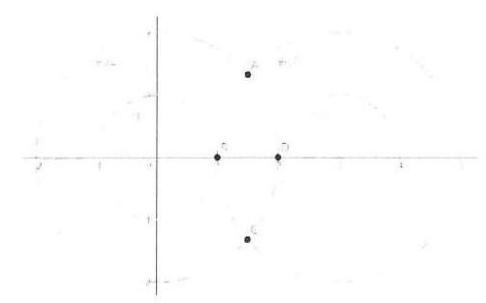
\includegraphics[max width=0.4\textwidth]{images/bo_d5jma53ef24c73bll4ig_149_294_780_486_303_0.jpg}
\end{center}
\hspace*{3em} 

即 \(\left( {\left( {a - b}\right)  - \left( {c - d}\right) \mathrm{i}}\right) \left( {\left( {a - b}\right)  + \left( {c - d}\right) \mathrm{i}}\right)  = 9\) ,

即 \({\left( a - b\right) }^{2} + {\left( c - d\right) }^{2} = 9\) ,

故 \({w}_{1}\text{ 、 }{w}_{2}\) 对应平面内距离为 3 的点,

因为 \(\left| {{w}_{i} - {z}_{j}}\right|  \in  \{ 1,2\}\) ,所以 \({z}_{i}\) 与 \({w}_{1}\text{ 、 }{w}_{2}\) 对应的点的距离为 1 或 2,

构成了 4 个点 \(\left( {A,B,C,D}\right)\) ,故 \(n\) 的最大值为 4 .

【练习】7. (艺扬飞翔) 平面单位向量 \(\overrightarrow{{\mathrm{e}}_{1}},\overrightarrow{{\mathrm{e}}_{2}}\) 满足: 存在点 \(Q\) ,使得对于任意 \(m \in  \left\lbrack  {1,4}\right\rbrack\) ,存在 \(n \in  \left\lbrack  {0\text{ , }}\right\rbrack \; + \infty )\) ，有 \(\overrightarrow{OP} = m\overrightarrow{{\mathrm{e}}_{1}} + n\overrightarrow{{\mathrm{e}}_{2}}\) ，且 \(\left| {PQ}\right|  = 1\) ，则 \(\overrightarrow{{\mathrm{e}}_{1}} \cdot  \overrightarrow{{\mathrm{e}}_{2}}\) 的取值范围是\_\_\_\_\_.

【答案】 \(\left\lbrack  {-1, - \frac{\sqrt{5}}{3}}\right\rbrack   \cup  \left\lbrack  {\frac{\sqrt{5}}{3},1}\right\rbrack\)

【解析】听我讲吧 \(= 0 =\) ,极端情况转化为两条射线间距离等于 2

【练习】8. (艺扬飞翔) 已知平面向量 \(\overrightarrow{a},\overrightarrow{b},\left| \overrightarrow{a}\right|  = 1,\left| \overrightarrow{b}\right|  = 2,\overrightarrow{a} \cdot  \overrightarrow{b} = 0,\Omega  = \left\{  {\overrightarrow{u} \mid  \left( {\overrightarrow{u} - \overrightarrow{a}}\right)  \cdot  \left( {\overrightarrow{u} - \overrightarrow{b}}\right)  < r}\right\}\) 是非空集合,若存在平面向量 \(\overrightarrow{c} \in  \Omega\) ,使得对于任意 \(s \in  R\) ,都存在 \(t \in  \left\lbrack  {0,1}\right\rbrack\) ,满足 \(\left( {\overrightarrow{c} - s\overrightarrow{a}}\right)  \cdot  \left( {\overrightarrow{c} - t\overrightarrow{b}}\right) \; < 0\) ，则实数 \(r\) 的取值范围是\_\_\_\_\_.

【答案】 \(\left( {-1, + \infty }\right)\)

【解析】听我讲吧 \(= 0 =\) ,极端情况转化为圆与 \(y\) 轴有公共点即可

【练习】9. 已知向量 \(\overrightarrow{b},\overrightarrow{c}\) 满足 \(\left| {\overrightarrow{b} - \overrightarrow{c}}\right|  = 1\) ，向量 \(\overrightarrow{{a}_{i}}\left( {1 \leq  i \leq  n,n \in  N,n \geq  1}\right)\) ，满足 \(\left| {\overrightarrow{{a}_{i}} - \overrightarrow{b}}\right|  = 1\) 或 \(\left| {\overrightarrow{{a}_{i}} - \overrightarrow{c}}\right|  = 1\) 且 \(\left| {{\overrightarrow{a}}_{i} - {\overrightarrow{a}}_{j}}\right|  \geq  1\) 对任意 \(1 \leq  \mathrm{i} < j \leq  n\) 成立. 则 \(n\) 的最大值为\_\_\_\_\_.

【答案】 10

【解析】设 \(\overrightarrow{b} = \overrightarrow{OB},\overrightarrow{c} = \overrightarrow{OC},{\overrightarrow{a}}_{i} = \overrightarrow{O{A}_{i}}\) ,

\begin{center}
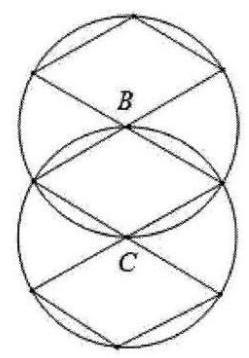
\includegraphics[max width=0.2\textwidth]{images/bo_d5jma53ef24c73bll4ig_150_296_441_249_358_0.jpg}
\end{center}
\hspace*{3em} 

则 \(\left| {\overrightarrow{b} - \overrightarrow{c}}\right|  = \left| \overrightarrow{CB}\right|  = 1,\left| {{\overrightarrow{a}}_{i} - \overrightarrow{b}}\right|  = \left| {\overrightarrow{O{A}_{i}} - \overrightarrow{OB}}\right|  = \left| \overrightarrow{B{A}_{i}}\right|  = 1,\left| {{\overrightarrow{a}}_{i} - \overrightarrow{c}}\right|  = \left| {\overrightarrow{O{A}_{i}} - \overrightarrow{OC}}\right|  = \left| \overrightarrow{C{A}_{i}}\right|  = 1\) ,

所以 \({A}_{1},B,C\) 三点共线，且 \({A}_{1}\) 在 \(B,C\) 之间，因为 \(\left| {{\overrightarrow{a}}_{j} - {\overrightarrow{a}}_{j}}\right|  \geq  1\) ，所以 \(\left| \overrightarrow{{A}_{i}{A}_{j}}\right|  \geq  1\) ，

即 \({A}_{1},{A}_{2},\cdots ,{A}_{n}\) ,中任意两点之间的距离不小于 1,因为 \(\left| {\overrightarrow{b} - \overrightarrow{c}}\right|  = \left| \overrightarrow{CB}\right|  = 1\) ,

作出图像,观察易得, \(n\) 的最大值为 10 .
\end{document}